% Options for packages loaded elsewhere
\PassOptionsToPackage{unicode}{hyperref}
\PassOptionsToPackage{hyphens}{url}
\PassOptionsToPackage{dvipsnames,svgnames,x11names}{xcolor}
%
\documentclass[
  letterpaper,
  DIV=11,
  numbers=noendperiod]{scrreprt}

\usepackage{amsmath,amssymb}
\usepackage{iftex}
\ifPDFTeX
  \usepackage[T1]{fontenc}
  \usepackage[utf8]{inputenc}
  \usepackage{textcomp} % provide euro and other symbols
\else % if luatex or xetex
  \usepackage{unicode-math}
  \defaultfontfeatures{Scale=MatchLowercase}
  \defaultfontfeatures[\rmfamily]{Ligatures=TeX,Scale=1}
\fi
\usepackage{lmodern}
\ifPDFTeX\else  
    % xetex/luatex font selection
\fi
% Use upquote if available, for straight quotes in verbatim environments
\IfFileExists{upquote.sty}{\usepackage{upquote}}{}
\IfFileExists{microtype.sty}{% use microtype if available
  \usepackage[]{microtype}
  \UseMicrotypeSet[protrusion]{basicmath} % disable protrusion for tt fonts
}{}
\makeatletter
\@ifundefined{KOMAClassName}{% if non-KOMA class
  \IfFileExists{parskip.sty}{%
    \usepackage{parskip}
  }{% else
    \setlength{\parindent}{0pt}
    \setlength{\parskip}{6pt plus 2pt minus 1pt}}
}{% if KOMA class
  \KOMAoptions{parskip=half}}
\makeatother
\usepackage{xcolor}
\setlength{\emergencystretch}{3em} % prevent overfull lines
\setcounter{secnumdepth}{5}
% Make \paragraph and \subparagraph free-standing
\ifx\paragraph\undefined\else
  \let\oldparagraph\paragraph
  \renewcommand{\paragraph}[1]{\oldparagraph{#1}\mbox{}}
\fi
\ifx\subparagraph\undefined\else
  \let\oldsubparagraph\subparagraph
  \renewcommand{\subparagraph}[1]{\oldsubparagraph{#1}\mbox{}}
\fi

\usepackage{color}
\usepackage{fancyvrb}
\newcommand{\VerbBar}{|}
\newcommand{\VERB}{\Verb[commandchars=\\\{\}]}
\DefineVerbatimEnvironment{Highlighting}{Verbatim}{commandchars=\\\{\}}
% Add ',fontsize=\small' for more characters per line
\usepackage{framed}
\definecolor{shadecolor}{RGB}{241,243,245}
\newenvironment{Shaded}{\begin{snugshade}}{\end{snugshade}}
\newcommand{\AlertTok}[1]{\textcolor[rgb]{0.68,0.00,0.00}{#1}}
\newcommand{\AnnotationTok}[1]{\textcolor[rgb]{0.37,0.37,0.37}{#1}}
\newcommand{\AttributeTok}[1]{\textcolor[rgb]{0.40,0.45,0.13}{#1}}
\newcommand{\BaseNTok}[1]{\textcolor[rgb]{0.68,0.00,0.00}{#1}}
\newcommand{\BuiltInTok}[1]{\textcolor[rgb]{0.00,0.23,0.31}{#1}}
\newcommand{\CharTok}[1]{\textcolor[rgb]{0.13,0.47,0.30}{#1}}
\newcommand{\CommentTok}[1]{\textcolor[rgb]{0.37,0.37,0.37}{#1}}
\newcommand{\CommentVarTok}[1]{\textcolor[rgb]{0.37,0.37,0.37}{\textit{#1}}}
\newcommand{\ConstantTok}[1]{\textcolor[rgb]{0.56,0.35,0.01}{#1}}
\newcommand{\ControlFlowTok}[1]{\textcolor[rgb]{0.00,0.23,0.31}{#1}}
\newcommand{\DataTypeTok}[1]{\textcolor[rgb]{0.68,0.00,0.00}{#1}}
\newcommand{\DecValTok}[1]{\textcolor[rgb]{0.68,0.00,0.00}{#1}}
\newcommand{\DocumentationTok}[1]{\textcolor[rgb]{0.37,0.37,0.37}{\textit{#1}}}
\newcommand{\ErrorTok}[1]{\textcolor[rgb]{0.68,0.00,0.00}{#1}}
\newcommand{\ExtensionTok}[1]{\textcolor[rgb]{0.00,0.23,0.31}{#1}}
\newcommand{\FloatTok}[1]{\textcolor[rgb]{0.68,0.00,0.00}{#1}}
\newcommand{\FunctionTok}[1]{\textcolor[rgb]{0.28,0.35,0.67}{#1}}
\newcommand{\ImportTok}[1]{\textcolor[rgb]{0.00,0.46,0.62}{#1}}
\newcommand{\InformationTok}[1]{\textcolor[rgb]{0.37,0.37,0.37}{#1}}
\newcommand{\KeywordTok}[1]{\textcolor[rgb]{0.00,0.23,0.31}{#1}}
\newcommand{\NormalTok}[1]{\textcolor[rgb]{0.00,0.23,0.31}{#1}}
\newcommand{\OperatorTok}[1]{\textcolor[rgb]{0.37,0.37,0.37}{#1}}
\newcommand{\OtherTok}[1]{\textcolor[rgb]{0.00,0.23,0.31}{#1}}
\newcommand{\PreprocessorTok}[1]{\textcolor[rgb]{0.68,0.00,0.00}{#1}}
\newcommand{\RegionMarkerTok}[1]{\textcolor[rgb]{0.00,0.23,0.31}{#1}}
\newcommand{\SpecialCharTok}[1]{\textcolor[rgb]{0.37,0.37,0.37}{#1}}
\newcommand{\SpecialStringTok}[1]{\textcolor[rgb]{0.13,0.47,0.30}{#1}}
\newcommand{\StringTok}[1]{\textcolor[rgb]{0.13,0.47,0.30}{#1}}
\newcommand{\VariableTok}[1]{\textcolor[rgb]{0.07,0.07,0.07}{#1}}
\newcommand{\VerbatimStringTok}[1]{\textcolor[rgb]{0.13,0.47,0.30}{#1}}
\newcommand{\WarningTok}[1]{\textcolor[rgb]{0.37,0.37,0.37}{\textit{#1}}}

\providecommand{\tightlist}{%
  \setlength{\itemsep}{0pt}\setlength{\parskip}{0pt}}\usepackage{longtable,booktabs,array}
\usepackage{calc} % for calculating minipage widths
% Correct order of tables after \paragraph or \subparagraph
\usepackage{etoolbox}
\makeatletter
\patchcmd\longtable{\par}{\if@noskipsec\mbox{}\fi\par}{}{}
\makeatother
% Allow footnotes in longtable head/foot
\IfFileExists{footnotehyper.sty}{\usepackage{footnotehyper}}{\usepackage{footnote}}
\makesavenoteenv{longtable}
\usepackage{graphicx}
\makeatletter
\def\maxwidth{\ifdim\Gin@nat@width>\linewidth\linewidth\else\Gin@nat@width\fi}
\def\maxheight{\ifdim\Gin@nat@height>\textheight\textheight\else\Gin@nat@height\fi}
\makeatother
% Scale images if necessary, so that they will not overflow the page
% margins by default, and it is still possible to overwrite the defaults
% using explicit options in \includegraphics[width, height, ...]{}
\setkeys{Gin}{width=\maxwidth,height=\maxheight,keepaspectratio}
% Set default figure placement to htbp
\makeatletter
\def\fps@figure{htbp}
\makeatother
% definitions for citeproc citations
\NewDocumentCommand\citeproctext{}{}
\NewDocumentCommand\citeproc{mm}{%
  \begingroup\def\citeproctext{#2}\cite{#1}\endgroup}
\makeatletter
 % allow citations to break across lines
 \let\@cite@ofmt\@firstofone
 % avoid brackets around text for \cite:
 \def\@biblabel#1{}
 \def\@cite#1#2{{#1\if@tempswa , #2\fi}}
\makeatother
\newlength{\cslhangindent}
\setlength{\cslhangindent}{1.5em}
\newlength{\csllabelwidth}
\setlength{\csllabelwidth}{3em}
\newenvironment{CSLReferences}[2] % #1 hanging-indent, #2 entry-spacing
 {\begin{list}{}{%
  \setlength{\itemindent}{0pt}
  \setlength{\leftmargin}{0pt}
  \setlength{\parsep}{0pt}
  % turn on hanging indent if param 1 is 1
  \ifodd #1
   \setlength{\leftmargin}{\cslhangindent}
   \setlength{\itemindent}{-1\cslhangindent}
  \fi
  % set entry spacing
  \setlength{\itemsep}{#2\baselineskip}}}
 {\end{list}}
\usepackage{calc}
\newcommand{\CSLBlock}[1]{\hfill\break\parbox[t]{\linewidth}{\strut\ignorespaces#1\strut}}
\newcommand{\CSLLeftMargin}[1]{\parbox[t]{\csllabelwidth}{\strut#1\strut}}
\newcommand{\CSLRightInline}[1]{\parbox[t]{\linewidth - \csllabelwidth}{\strut#1\strut}}
\newcommand{\CSLIndent}[1]{\hspace{\cslhangindent}#1}

\KOMAoption{captions}{tableheading}
\makeatletter
\@ifpackageloaded{tcolorbox}{}{\usepackage[skins,breakable]{tcolorbox}}
\@ifpackageloaded{fontawesome5}{}{\usepackage{fontawesome5}}
\definecolor{quarto-callout-color}{HTML}{909090}
\definecolor{quarto-callout-note-color}{HTML}{0758E5}
\definecolor{quarto-callout-important-color}{HTML}{CC1914}
\definecolor{quarto-callout-warning-color}{HTML}{EB9113}
\definecolor{quarto-callout-tip-color}{HTML}{00A047}
\definecolor{quarto-callout-caution-color}{HTML}{FC5300}
\definecolor{quarto-callout-color-frame}{HTML}{acacac}
\definecolor{quarto-callout-note-color-frame}{HTML}{4582ec}
\definecolor{quarto-callout-important-color-frame}{HTML}{d9534f}
\definecolor{quarto-callout-warning-color-frame}{HTML}{f0ad4e}
\definecolor{quarto-callout-tip-color-frame}{HTML}{02b875}
\definecolor{quarto-callout-caution-color-frame}{HTML}{fd7e14}
\makeatother
\makeatletter
\@ifpackageloaded{bookmark}{}{\usepackage{bookmark}}
\makeatother
\makeatletter
\@ifpackageloaded{caption}{}{\usepackage{caption}}
\AtBeginDocument{%
\ifdefined\contentsname
  \renewcommand*\contentsname{Table of contents}
\else
  \newcommand\contentsname{Table of contents}
\fi
\ifdefined\listfigurename
  \renewcommand*\listfigurename{List of Figures}
\else
  \newcommand\listfigurename{List of Figures}
\fi
\ifdefined\listtablename
  \renewcommand*\listtablename{List of Tables}
\else
  \newcommand\listtablename{List of Tables}
\fi
\ifdefined\figurename
  \renewcommand*\figurename{Figure}
\else
  \newcommand\figurename{Figure}
\fi
\ifdefined\tablename
  \renewcommand*\tablename{Table}
\else
  \newcommand\tablename{Table}
\fi
}
\@ifpackageloaded{float}{}{\usepackage{float}}
\floatstyle{ruled}
\@ifundefined{c@chapter}{\newfloat{codelisting}{h}{lop}}{\newfloat{codelisting}{h}{lop}[chapter]}
\floatname{codelisting}{Listing}
\newcommand*\listoflistings{\listof{codelisting}{List of Listings}}
\makeatother
\makeatletter
\makeatother
\makeatletter
\@ifpackageloaded{caption}{}{\usepackage{caption}}
\@ifpackageloaded{subcaption}{}{\usepackage{subcaption}}
\makeatother
\ifLuaTeX
  \usepackage{selnolig}  % disable illegal ligatures
\fi
\usepackage{bookmark}

\IfFileExists{xurl.sty}{\usepackage{xurl}}{} % add URL line breaks if available
\urlstyle{same} % disable monospaced font for URLs
\hypersetup{
  pdftitle={Hyperparameter Tuning Cookbook},
  pdfauthor={Thomas Bartz-Beielstein},
  colorlinks=true,
  linkcolor={blue},
  filecolor={Maroon},
  citecolor={Blue},
  urlcolor={Blue},
  pdfcreator={LaTeX via pandoc}}

\title{Hyperparameter Tuning Cookbook}
\usepackage{etoolbox}
\makeatletter
\providecommand{\subtitle}[1]{% add subtitle to \maketitle
  \apptocmd{\@title}{\par {\large #1 \par}}{}{}
}
\makeatother
\subtitle{A guide for scikit-learn, PyTorch, river, and spotPython}
\author{Thomas Bartz-Beielstein}
\date{Mar 11, 2024}

\begin{document}
\maketitle

\renewcommand*\contentsname{Table of contents}
{
\hypersetup{linkcolor=}
\setcounter{tocdepth}{2}
\tableofcontents
}
\bookmarksetup{startatroot}

\chapter*{Preface}\label{preface}
\addcontentsline{toc}{chapter}{Preface}

\markboth{Preface}{Preface}

\begin{quote}
This document provides a comprehensive guide to hyperparameter tuning
using spotPython for scikit-learn, scipy-optimize, River, and PyTorch.
The first part introduces fundamental ideas from optimization. The
second part discusses numerical issues and introduces spotPython's
surrogate model-based optimization process. The thirs part focuses on
hyperparameter tuning. Several case studies are presented, including
hyperparameter tuning for sklearn models such as Support Vector
Classification, Random Forests, Gradient Boosting (XGB), and K-nearest
neighbors (KNN), as well as a Hoeffding Adaptive Tree Regressor from
river. The integration of spotPython into the PyTorch and PyTorch
Lightning training workflow is also discussed. With a hands-on approach
and step-by-step explanations, this cookbook serves as a practical
starting point for anyone interested in hyperparameter tuning with
Python. Highlights include the interplay between Tensorboard, PyTorch
Lightning, spotPython, spotRiver, and River. This publication is under
development, with updates available on the corresponding webpage.
\end{quote}

\begin{tcolorbox}[enhanced jigsaw, rightrule=.15mm, opacitybacktitle=0.6, coltitle=black, bottomrule=.15mm, bottomtitle=1mm, title=\textcolor{quarto-callout-important-color}{\faExclamation}\hspace{0.5em}{Important: This book is still under development.}, left=2mm, colframe=quarto-callout-important-color-frame, titlerule=0mm, toptitle=1mm, arc=.35mm, colbacktitle=quarto-callout-important-color!10!white, breakable, toprule=.15mm, opacityback=0, leftrule=.75mm, colback=white]

The most recent version of this book is available at
\url{https://sequential-parameter-optimization.github.io/Hyperparameter-Tuning-Cookbook/}

\end{tcolorbox}

\section*{Book Structure}\label{book-structure}
\addcontentsline{toc}{section}{Book Structure}

\markright{Book Structure}

This document is structured in three parts. The first part presents an
introduction to optimization. The second part describes numerical
methods, and the third part presents hyperparameter tuning.

\begin{tcolorbox}[enhanced jigsaw, rightrule=.15mm, opacitybacktitle=0.6, coltitle=black, bottomrule=.15mm, bottomtitle=1mm, title=\textcolor{quarto-callout-tip-color}{\faLightbulb}\hspace{0.5em}{Hyperparameter Tuning Reference}, left=2mm, colframe=quarto-callout-tip-color-frame, titlerule=0mm, toptitle=1mm, arc=.35mm, colbacktitle=quarto-callout-tip-color!10!white, breakable, toprule=.15mm, opacityback=0, leftrule=.75mm, colback=white]

\begin{itemize}
\tightlist
\item
  The open access book Bartz et al. (2022) provides a comprehensive
  overview of hyperparameter tuning. It can be downloaded from
  \url{https://link.springer.com/book/10.1007/978-981-19-5170-1}.
\end{itemize}

\end{tcolorbox}

\begin{tcolorbox}[enhanced jigsaw, rightrule=.15mm, opacitybacktitle=0.6, coltitle=black, bottomrule=.15mm, bottomtitle=1mm, title=\textcolor{quarto-callout-note-color}{\faInfo}\hspace{0.5em}{Note}, left=2mm, colframe=quarto-callout-note-color-frame, titlerule=0mm, toptitle=1mm, arc=.35mm, colbacktitle=quarto-callout-note-color!10!white, breakable, toprule=.15mm, opacityback=0, leftrule=.75mm, colback=white]

The \texttt{.ipynb} notebook (Bartz-Beielstein 2023) is updated
regularly and reflects updates and changes in the \texttt{spotPython}
package. It can be downloaded from
\url{https://github.com/sequential-parameter-optimization/spotPython/blob/main/notebooks/14_spot_ray_hpt_torch_cifar10.ipynb}.

\end{tcolorbox}

\section*{Software Used in this Book}\label{software-used-in-this-book}
\addcontentsline{toc}{section}{Software Used in this Book}

\markright{Software Used in this Book}

\href{https://scikit-learn.org}{scikit-learn} is a Python module for
machine learning built on top of SciPy and is distributed under the
3-Clause BSD license. The project was started in 2007 by David
Cournapeau as a Google Summer of Code project, and since then many
volunteers have contributed.

\href{https://pytorch.org}{PyTorch} is an optimized tensor library for
deep learning using GPUs and CPUs.
\href{https://lightning.ai/docs/pytorch/latest/}{Lightning} is a
lightweight PyTorch wrapper for high-performance AI research. It allows
you to decouple the research from the engineering.

\href{https://riverml.xyz}{River} is a Python library for online machine
learning. It is designed to be used in real-world environments, where
not all data is available at once, but streaming in.

\href{https://github.com/sequential-parameter-optimization/spotPython}{spotPython}
(``Sequential Parameter Optimization Toolbox in Python'') is the Python
version of the well-known hyperparameter tuner SPOT, which has been
developed in the R programming environment for statistical analysis for
over a decade. The related open-access book is available here:
\href{https://link.springer.com/book/10.1007/978-981-19-5170-1}{Hyperparameter
Tuning for Machine and Deep Learning with R---A Practical Guide}.

\href{https://github.com/sequential-parameter-optimization/spotRiver}{spotRiver}
provides an interface between
\href{https://github.com/sequential-parameter-optimization/spotPython}{spotPython}
and \href{https://riverml.xyz}{River}.

\section*{Citation}\label{citation}
\addcontentsline{toc}{section}{Citation}

\markright{Citation}

If this document has been useful to you and you wish to cite it in a
scientific publication, please refer to the following paper, which can
be found on arXiv: \url{https://arxiv.org/abs/2307.10262}.

\begin{Shaded}
\begin{Highlighting}[]
\NormalTok{@ARTICLE\{bart23iArXiv,}
\NormalTok{      author = \{\{Bartz{-}Beielstein\}, Thomas\},}
\NormalTok{      title = "\{Hyperparameter Tuning Cookbook:}
\NormalTok{          A guide for scikit{-}learn, PyTorch, river, and spotPython\}",}
\NormalTok{     journal = \{arXiv e{-}prints\},}
\NormalTok{    keywords = \{Computer Science {-} Machine Learning,}
\NormalTok{      Computer Science {-} Artificial Intelligence, 90C26, I.2.6, G.1.6\},}
\NormalTok{         year = 2023,}
\NormalTok{        month = jul,}
\NormalTok{          eid = \{arXiv:2307.10262\},}
\NormalTok{        pages = \{arXiv:2307.10262\},}
\NormalTok{          doi = \{10.48550/arXiv.2307.10262\},}
\NormalTok{archivePrefix = \{arXiv\},}
\NormalTok{       eprint = \{2307.10262\},}
\NormalTok{ primaryClass = \{cs.LG\},}
\NormalTok{       adsurl = \{https://ui.adsabs.harvard.edu/abs/2023arXiv230710262B\},}
\NormalTok{      adsnote = \{Provided by the SAO/NASA Astrophysics Data System\}}
\NormalTok{\}}

\end{Highlighting}
\end{Shaded}

\part{Optimization}

\chapter{Introduction: Optimization}\label{introduction-optimization}

\section{Optimization, Simulation, and Surrogate
Modeling}\label{optimization-simulation-and-surrogate-modeling}

\begin{itemize}
\tightlist
\item
  We will consider the interplay between

  \begin{itemize}
  \tightlist
  \item
    mathematical models,
  \item
    numerical approximation,
  \item
    simulation,
  \item
    computer experiments, and
  \item
    field data
  \end{itemize}
\item
  Experimental design will play a key role in our developments, but not
  in the classical regression and response surface methodology sense
\item
  Challenging real-data/real-simulation examples benefiting from modern
  surrogate modeling methodology
\item
  We will consider the classical, response surface methodology (RSM)
  approach, and then move on to more modern approaches
\item
  All approaches are based on surrogates
\end{itemize}

\section{Surrogates}\label{surrogates}

\begin{itemize}
\tightlist
\item
  Gathering data is \textbf{expensive}, and sometimes getting exactly
  the data you want is impossible or unethical
\item
  \textbf{Surrogate}: substitute for the real thing
\item
  In statistics, draws from predictive equations derived from a fitted
  model can act as a surrogate for the data-generating mechanism
\item
  Benefits of the surrogate approach:

  \begin{itemize}
  \tightlist
  \item
    Surrogate could represent a cheaper way to explore relationships,
    and entertain ``what ifs?''
  \item
    Surrogates favor faithful yet pragmatic reproduction of dynamics:

    \begin{itemize}
    \tightlist
    \item
      interpretation,
    \item
      establishing causality, or
    \item
      identification
    \end{itemize}
  \item
    Many numerical simulators are \textbf{deterministic}, whereas field
    observations are noisy or have measurement error
  \end{itemize}
\end{itemize}

\subsection{Costs of Simulation}\label{costs-of-simulation}

\begin{itemize}
\tightlist
\item
  Computer simulations are generally cheaper (but not always!) than
  physical observation
\item
  Some computer simulations can be just as expensive as field
  experimentation, but computer modeling is regarded as easier because:

  \begin{itemize}
  \tightlist
  \item
    the experimental apparatus is better understood
  \item
    more aspects may be controlled.
  \end{itemize}
\end{itemize}

\subsection{Mathematical Models and
Meta-Models}\label{mathematical-models-and-meta-models}

\begin{itemize}
\tightlist
\item
  Use of mathematical models leveraging numerical solvers has been
  commonplace for some time
\item
  Mathematical models became more complex, requiring more resources to
  simulate/solve numerically
\item
  Practitioners increasingly relied on \textbf{meta-models} built off of
  limited simulation campaigns
\end{itemize}

\subsection{Surrogates = Trained
Meta-models}\label{surrogates-trained-meta-models}

\begin{itemize}
\tightlist
\item
  Data collected via expensive computer evaluations tuned flexible
  functional forms that could be used in lieu of further simulation to

  \begin{itemize}
  \tightlist
  \item
    save money or computational resources;
  \item
    cope with an inability to perform future runs (expired licenses,
    off-line or over-impacted supercomputers)
  \end{itemize}
\item
  Trained meta-models became known as \textbf{surrogates}
\end{itemize}

\subsection{Computer Experiments}\label{computer-experiments}

\begin{itemize}
\tightlist
\item
  \textbf{Computer experiment}: design, running, and fitting
  meta-models.

  \begin{itemize}
  \tightlist
  \item
    Like an ordinary statistical experiment, except the data are
    generated by computer codes rather than physical or field
    observations, or surveys
  \end{itemize}
\item
  \textbf{Surrogate modeling} is statistical modeling of computer
  experiments
\end{itemize}

\subsection{Limits of Mathematical
Modeling}\label{limits-of-mathematical-modeling}

\begin{itemize}
\tightlist
\item
  Mathematical biologists, economists and others had reached the limit
  of equilibrium-based mathematical modeling with cute closed-form
  solutions
\item
  \textbf{Stochastic simulations replace deterministic solvers} based on
  FEM, Navier--Stokes or Euler methods
\item
  Agent-based simulation models are used to explore predator-prey
  (Lotka--Voltera) dynamics, spread of disease, management of inventory
  or patients in health insurance markets
\item
  Consequence: the distinction between surrogate and statistical model
  is all but gone
\end{itemize}

\subsection{Example: Why Computer Simulations are
Necessary}\label{example-why-computer-simulations-are-necessary}

\begin{itemize}
\tightlist
\item
  You can't seed a real community with Ebola and watch what happens
\item
  If there's (real) field data, say on a historical epidemic, further
  experimentation may be almost entirely limited to the mathematical and
  computer modeling side
\item
  Classical statistical methods offer little guidance
\end{itemize}

\subsection{Simulation Requirements}\label{simulation-requirements}

\begin{itemize}
\tightlist
\item
  Simulation should

  \begin{itemize}
  \tightlist
  \item
    enable rich \textbf{diagnostics} to help criticize that models
  \item
    \textbf{understanding} its sensitivity to inputs and other
    configurations
  \item
    providing the ability to \textbf{optimize} and
  \item
    refine both \textbf{automatically} and with expert intervention
  \end{itemize}
\item
  And it has to do all that while remaining \textbf{computationally
  tractable}
\item
  One perspective is so-called \textbf{response surface methods} (RSMs):
\item
  a poster child from industrial statistics' heyday, well before
  information technology became a dominant industry
\end{itemize}

\begin{tcolorbox}[enhanced jigsaw, rightrule=.15mm, opacitybacktitle=0.6, coltitle=black, bottomrule=.15mm, bottomtitle=1mm, title=\textcolor{quarto-callout-important-color}{\faExclamation}\hspace{0.5em}{Goals}, left=2mm, colframe=quarto-callout-important-color-frame, titlerule=0mm, toptitle=1mm, arc=.35mm, colbacktitle=quarto-callout-important-color!10!white, breakable, toprule=.15mm, opacityback=0, leftrule=.75mm, colback=white]

\begin{itemize}
\tightlist
\item
  How to choose models and optimizers for solving real-world problems
\item
  How to use simulation to understand and improve processes
\end{itemize}

\end{tcolorbox}

\section{Jupyter Notebook}\label{jupyter-notebook}

\begin{tcolorbox}[enhanced jigsaw, rightrule=.15mm, opacitybacktitle=0.6, coltitle=black, bottomrule=.15mm, bottomtitle=1mm, title=\textcolor{quarto-callout-note-color}{\faInfo}\hspace{0.5em}{Note}, left=2mm, colframe=quarto-callout-note-color-frame, titlerule=0mm, toptitle=1mm, arc=.35mm, colbacktitle=quarto-callout-note-color!10!white, breakable, toprule=.15mm, opacityback=0, leftrule=.75mm, colback=white]

\begin{itemize}
\tightlist
\item
  The Jupyter-Notebook of this lecture is available on GitHub in the
  \href{https://github.com/sequential-parameter-optimization/Hyperparameter-Tuning-Cookbook/blob/main/001_optimization_surrogate.ipynb}{Hyperparameter-Tuning-Cookbook
  Repository}
\end{itemize}

\end{tcolorbox}

\chapter{Aircraft Wing Weight
Example}\label{aircraft-wing-weight-example}

\section{AWWE Equation}\label{awwe-equation}

\begin{itemize}
\tightlist
\item
  Example from Forrester et al.~
\item
  Understand the \textbf{weight} of an unpainted light aircraft wing as
  a function of nine design and operational parameters:
\end{itemize}

\[ W = 0.036 S_W^{0.758} \times W_{fw}^{0.0035} \left( \frac{A}{\cos^2 \Lambda} \right)^{0.6} \times  q^{0.006}  \times \lambda^{0.04} \]
\[ \times \left( \frac{100 R_{tc}}{\cos \Lambda} \right)^{-0.3} \times (N_z W_{dg})^{0.49}\]

\section{AWWE Parameters and Equations (Part
1)}\label{awwe-parameters-and-equations-part-1}

\begin{longtable}[]{@{}
  >{\raggedright\arraybackslash}p{(\columnwidth - 8\tabcolsep) * \real{0.1392}}
  >{\raggedright\arraybackslash}p{(\columnwidth - 8\tabcolsep) * \real{0.5063}}
  >{\raggedright\arraybackslash}p{(\columnwidth - 8\tabcolsep) * \real{0.1266}}
  >{\raggedright\arraybackslash}p{(\columnwidth - 8\tabcolsep) * \real{0.1139}}
  >{\raggedright\arraybackslash}p{(\columnwidth - 8\tabcolsep) * \real{0.1139}}@{}}
\caption{Aircraft Wing Weight Parameters}\label{tbl-awwe}\tabularnewline
\toprule\noalign{}
\begin{minipage}[b]{\linewidth}\raggedright
Symbol
\end{minipage} & \begin{minipage}[b]{\linewidth}\raggedright
Parameter
\end{minipage} & \begin{minipage}[b]{\linewidth}\raggedright
Baseline
\end{minipage} & \begin{minipage}[b]{\linewidth}\raggedright
Minimum
\end{minipage} & \begin{minipage}[b]{\linewidth}\raggedright
Maximum
\end{minipage} \\
\midrule\noalign{}
\endfirsthead
\toprule\noalign{}
\begin{minipage}[b]{\linewidth}\raggedright
Symbol
\end{minipage} & \begin{minipage}[b]{\linewidth}\raggedright
Parameter
\end{minipage} & \begin{minipage}[b]{\linewidth}\raggedright
Baseline
\end{minipage} & \begin{minipage}[b]{\linewidth}\raggedright
Minimum
\end{minipage} & \begin{minipage}[b]{\linewidth}\raggedright
Maximum
\end{minipage} \\
\midrule\noalign{}
\endhead
\bottomrule\noalign{}
\endlastfoot
\(S_W\) & Wing area (\(ft^2\)) & 174 & 150 & 200 \\
\(W_{fw}\) & Weight of fuel in wing (lb) & 252 & 220 & 300 \\
\(A\) & Aspect ratio & 7.52 & 6 & 10 \\
\(\Lambda\) & Quarter-chord sweep (deg) & 0 & -10 & 10 \\
\(q\) & Dynamic pressure at cruise (\(lb/ft^2\)) & 34 & 16 & 45 \\
\(\lambda\) & Taper ratio & 0.672 & 0.5 & 1 \\
\(R_{tc}\) & Aerofoil thickness to chord ratio & 0.12 & 0.08 & 0.18 \\
\(N_z\) & Ultimate load factor & 3.8 & 2.5 & 6 \\
\(W_{dg}\) & Flight design gross weight (lb) & 2000 & 1700 & 2500 \\
\(W_p\) & paint weight (lb/ft\^{}2) & 0.064 & 0.025 & 0.08 \\
\end{longtable}

The study begins with a baseline Cessna C172 Skyhawk Aircraft as its
reference point. It aims to investigate the impact of wing area and fuel
weight on the overall weight of the aircraft. Two crucial parameters in
this analysis are the aspect ratio (\(A\)), defined as the ratio of the
wing's length to the average chord (thickness of the airfoil), and the
taper ratio (\(\lambda\)), which represents the ratio of the maximum to
the minimum thickness of the airfoil or the maximum to minimum chord.

It's important to note that the equation used in this context is not a
computer simulation but will be treated as one for the purpose of
illustration. This approach involves employing a true mathematical
equation, even if it's considered unknown, as a useful tool for
generating realistic settings to test the methodology. The functional
form of this equation was derived by ``calibrating'' known physical
relationships to curves obtained from existing aircraft data, as
referenced in Raymer 2012. Essentially, it acts as a surrogate for
actual measurements of aircraft weight.

Examining the mathematical properties of the AWWE (Aircraft Weight With
Wing Area and Fuel Weight Equation), it is evident that the response is
highly nonlinear concerning its inputs. While it's common to apply the
logarithm to simplify equations with complex exponents, even when
modeling the logarithm, which transforms powers into slope coefficients
and products into sums, the response remains nonlinear due to the
presence of trigonometric terms. Given the combination of nonlinearity
and high input dimension, simple linear and quadratic response surface
approximations are likely to be inadequate for this analysis.

\section{Goals: Understanding and
Optimization}\label{goals-understanding-and-optimization}

The primary goals of this study revolve around understanding and
optimization:

\begin{enumerate}
\def\labelenumi{\arabic{enumi}.}
\item
  \textbf{Understanding}: One of the straightforward objectives is to
  gain a deep understanding of the input-output relationships in this
  context. Given the global perspective implied by this setting, it
  becomes evident that a more sophisticated model is almost necessary.
  At this stage, let's focus on this specific scenario to establish a
  clear understanding.
\item
  \textbf{Optimization}: Another application of this analysis could be
  optimization. There may be an interest in minimizing the weight of the
  aircraft, but it's likely that there will be constraints in place. For
  example, the presence of wings with a nonzero area is essential for
  the aircraft to be capable of flying. In situations involving
  (constrained) optimization, a global perspective and, consequently,
  the use of flexible modeling are vital.
\end{enumerate}

The provided Python code serves as a genuine computer implementation
that ``solves'' a mathematical model. It accepts arguments encoded in
the unit cube, with defaults used to represent baseline settings, as
detailed in the table labeled as Table~\ref{tbl-awwe}. To map values
from the interval \([a, b]\) to the interval \([0, 1]\), the following
formula can be employed:

\[y = f(x) = \frac{x - a}{b - a}.\]

To reverse this mapping and obtain the original values, the formula
\[g(y) = a + (b - a) y\] can be used.

\begin{Shaded}
\begin{Highlighting}[]
\ImportTok{import}\NormalTok{ numpy }\ImportTok{as}\NormalTok{ np}

\KeywordTok{def}\NormalTok{ wingwt(Sw}\OperatorTok{=}\FloatTok{0.48}\NormalTok{, Wfw}\OperatorTok{=}\FloatTok{0.4}\NormalTok{, A}\OperatorTok{=}\FloatTok{0.38}\NormalTok{, L}\OperatorTok{=}\FloatTok{0.5}\NormalTok{, q}\OperatorTok{=}\FloatTok{0.62}\NormalTok{, l}\OperatorTok{=}\FloatTok{0.344}\NormalTok{,  Rtc}\OperatorTok{=}\FloatTok{0.4}\NormalTok{, Nz}\OperatorTok{=}\FloatTok{0.37}\NormalTok{, Wdg}\OperatorTok{=}\FloatTok{0.38}\NormalTok{):}
    \CommentTok{\# put coded inputs back on natural scale}
\NormalTok{    Sw }\OperatorTok{=}\NormalTok{ Sw }\OperatorTok{*}\NormalTok{ (}\DecValTok{200} \OperatorTok{{-}} \DecValTok{150}\NormalTok{) }\OperatorTok{+} \DecValTok{150} 
\NormalTok{    Wfw }\OperatorTok{=}\NormalTok{ Wfw }\OperatorTok{*}\NormalTok{ (}\DecValTok{300} \OperatorTok{{-}} \DecValTok{220}\NormalTok{) }\OperatorTok{+} \DecValTok{220} 
\NormalTok{    A }\OperatorTok{=}\NormalTok{ A }\OperatorTok{*}\NormalTok{ (}\DecValTok{10} \OperatorTok{{-}} \DecValTok{6}\NormalTok{) }\OperatorTok{+} \DecValTok{6} 
\NormalTok{    L }\OperatorTok{=}\NormalTok{ (L }\OperatorTok{*}\NormalTok{ (}\DecValTok{10} \OperatorTok{{-}}\NormalTok{ (}\OperatorTok{{-}}\DecValTok{10}\NormalTok{)) }\OperatorTok{{-}} \DecValTok{10}\NormalTok{) }\OperatorTok{*}\NormalTok{ np.pi}\OperatorTok{/}\DecValTok{180}
\NormalTok{    q }\OperatorTok{=}\NormalTok{ q }\OperatorTok{*}\NormalTok{ (}\DecValTok{45} \OperatorTok{{-}} \DecValTok{16}\NormalTok{) }\OperatorTok{+} \DecValTok{16} 
\NormalTok{    l }\OperatorTok{=}\NormalTok{ l }\OperatorTok{*}\NormalTok{ (}\DecValTok{1} \OperatorTok{{-}} \FloatTok{0.5}\NormalTok{) }\OperatorTok{+} \FloatTok{0.5}  
\NormalTok{    Rtc }\OperatorTok{=}\NormalTok{ Rtc }\OperatorTok{*}\NormalTok{ (}\FloatTok{0.18} \OperatorTok{{-}} \FloatTok{0.08}\NormalTok{) }\OperatorTok{+} \FloatTok{0.08}
\NormalTok{    Nz }\OperatorTok{=}\NormalTok{ Nz }\OperatorTok{*}\NormalTok{ (}\DecValTok{6} \OperatorTok{{-}} \FloatTok{2.5}\NormalTok{) }\OperatorTok{+} \FloatTok{2.5}
\NormalTok{    Wdg }\OperatorTok{=}\NormalTok{ Wdg}\OperatorTok{*}\NormalTok{(}\DecValTok{2500} \OperatorTok{{-}} \DecValTok{1700}\NormalTok{) }\OperatorTok{+} \DecValTok{1700}
    \CommentTok{\# calculation on natural scale}
\NormalTok{    W }\OperatorTok{=} \FloatTok{0.036} \OperatorTok{*}\NormalTok{ Sw}\OperatorTok{**}\FloatTok{0.758} \OperatorTok{*}\NormalTok{ Wfw}\OperatorTok{**}\FloatTok{0.0035} \OperatorTok{*}\NormalTok{ (A}\OperatorTok{/}\NormalTok{np.cos(L)}\OperatorTok{**}\DecValTok{2}\NormalTok{)}\OperatorTok{**}\FloatTok{0.6} \OperatorTok{*}\NormalTok{ q}\OperatorTok{**}\FloatTok{0.006} 
\NormalTok{    W }\OperatorTok{=}\NormalTok{ W }\OperatorTok{*}\NormalTok{ l}\OperatorTok{**}\FloatTok{0.04} \OperatorTok{*}\NormalTok{ (}\DecValTok{100}\OperatorTok{*}\NormalTok{Rtc}\OperatorTok{/}\NormalTok{np.cos(L))}\OperatorTok{**}\NormalTok{(}\OperatorTok{{-}}\FloatTok{0.3}\NormalTok{) }\OperatorTok{*}\NormalTok{ (Nz}\OperatorTok{*}\NormalTok{Wdg)}\OperatorTok{**}\NormalTok{(}\FloatTok{0.49}\NormalTok{)}
    \ControlFlowTok{return}\NormalTok{(W)}
\end{Highlighting}
\end{Shaded}

\section{Properties of the Python
``Solver''}\label{properties-of-the-python-solver}

The compute time required by the ``wingwt'' solver is extremely short
and can be considered trivial in terms of computational resources. The
approximation error is exceptionally small, effectively approaching
machine precision, which indicates the high accuracy of the solver's
results.

To simulate time-consuming evaluations, a deliberate delay is introduced
by incorporating a \texttt{sleep(3600)} command, which effectively
synthesizes a one-hour execution time for a particular evaluation.

Moving on to the AWWE visualization, plotting in two dimensions is
considerably simpler than dealing with nine dimensions. To aid in
creating visual representations, the code provided below establishes a
grid within the unit square to facilitate the generation of sliced
visuals. This involves generating a ``meshgrid'' as outlined in the
code.

\begin{Shaded}
\begin{Highlighting}[]
\ImportTok{import}\NormalTok{ numpy }\ImportTok{as}\NormalTok{ np}
\NormalTok{x }\OperatorTok{=}\NormalTok{ np.linspace(}\DecValTok{0}\NormalTok{, }\DecValTok{1}\NormalTok{, }\DecValTok{3}\NormalTok{)}
\NormalTok{y }\OperatorTok{=}\NormalTok{ np.linspace(}\DecValTok{0}\NormalTok{, }\DecValTok{1}\NormalTok{, }\DecValTok{3}\NormalTok{)}
\NormalTok{X, Y }\OperatorTok{=}\NormalTok{ np.meshgrid(x, y)}
\NormalTok{zp }\OperatorTok{=} \BuiltInTok{zip}\NormalTok{(np.ravel(X), np.ravel(Y))}
\BuiltInTok{list}\NormalTok{(zp)}
\end{Highlighting}
\end{Shaded}

\begin{verbatim}
[(0.0, 0.0),
 (0.5, 0.0),
 (1.0, 0.0),
 (0.0, 0.5),
 (0.5, 0.5),
 (1.0, 0.5),
 (0.0, 1.0),
 (0.5, 1.0),
 (1.0, 1.0)]
\end{verbatim}

The coding used to transform inputs from natural units is largely a
matter of taste, so long as it's easy to undo for reporting back on
original scales

\begin{Shaded}
\begin{Highlighting}[]
\OperatorTok{\%}\NormalTok{matplotlib inline}
\ImportTok{import}\NormalTok{ matplotlib.pyplot }\ImportTok{as}\NormalTok{ plt}
\CommentTok{\# plt.style.use(\textquotesingle{}seaborn{-}white\textquotesingle{})}
\ImportTok{import}\NormalTok{ numpy }\ImportTok{as}\NormalTok{ np}
\NormalTok{x }\OperatorTok{=}\NormalTok{ np.linspace(}\DecValTok{0}\NormalTok{, }\DecValTok{1}\NormalTok{, }\DecValTok{100}\NormalTok{)}
\NormalTok{y }\OperatorTok{=}\NormalTok{ np.linspace(}\DecValTok{0}\NormalTok{, }\DecValTok{1}\NormalTok{, }\DecValTok{100}\NormalTok{)}
\NormalTok{X, Y }\OperatorTok{=}\NormalTok{ np.meshgrid(x, y)}
\end{Highlighting}
\end{Shaded}

\section{\texorpdfstring{Plot 1: Load Factor (\(N_z\)) and Aspect Ratio
(\(A\))}{Plot 1: Load Factor (N\_z) and Aspect Ratio (A)}}\label{plot-1-load-factor-n_z-and-aspect-ratio-a}

We will vary \(N_z\) and \(A\), with other inputs fixed at their
baseline values.

\begin{Shaded}
\begin{Highlighting}[]
\NormalTok{z }\OperatorTok{=}\NormalTok{ wingwt(A }\OperatorTok{=}\NormalTok{ X, Nz }\OperatorTok{=}\NormalTok{ Y)}
\NormalTok{fig }\OperatorTok{=}\NormalTok{ plt.figure(figsize}\OperatorTok{=}\NormalTok{(}\FloatTok{7.}\NormalTok{, }\FloatTok{5.}\NormalTok{))}
\NormalTok{plt.contourf(X, Y, z, }\DecValTok{20}\NormalTok{, cmap}\OperatorTok{=}\StringTok{\textquotesingle{}jet\textquotesingle{}}\NormalTok{)}
\NormalTok{plt.xlabel(}\StringTok{"A"}\NormalTok{)}
\NormalTok{plt.ylabel(}\StringTok{"Nz"}\NormalTok{)}
\NormalTok{plt.title(}\StringTok{"Load factor (Nz) vs. Aspect Ratio (A)"}\NormalTok{)}
\NormalTok{plt.colorbar()}
\NormalTok{plt.show()}
\end{Highlighting}
\end{Shaded}

\includegraphics{002_awwe_files/figure-pdf/cell-5-output-1.pdf}

Contour plots can be refined, e.g., by adding explicit contour lines as
shown in the following figure.

\begin{Shaded}
\begin{Highlighting}[]
\NormalTok{contours }\OperatorTok{=}\NormalTok{ plt.contour(X, Y, z, }\DecValTok{4}\NormalTok{, colors}\OperatorTok{=}\StringTok{\textquotesingle{}black\textquotesingle{}}\NormalTok{)}
\NormalTok{plt.clabel(contours, inline}\OperatorTok{=}\VariableTok{True}\NormalTok{, fontsize}\OperatorTok{=}\DecValTok{8}\NormalTok{)}
\NormalTok{plt.xlabel(}\StringTok{"A"}\NormalTok{)}
\NormalTok{plt.ylabel(}\StringTok{"Nz"}\NormalTok{)}

\NormalTok{plt.imshow(z, extent}\OperatorTok{=}\NormalTok{[}\DecValTok{0}\NormalTok{, }\DecValTok{1}\NormalTok{, }\DecValTok{0}\NormalTok{, }\DecValTok{1}\NormalTok{], origin}\OperatorTok{=}\StringTok{\textquotesingle{}lower\textquotesingle{}}\NormalTok{,}
\NormalTok{           cmap}\OperatorTok{=}\StringTok{\textquotesingle{}jet\textquotesingle{}}\NormalTok{, alpha}\OperatorTok{=}\FloatTok{0.9}\NormalTok{)}
\NormalTok{plt.colorbar()}
\end{Highlighting}
\end{Shaded}

\includegraphics{002_awwe_files/figure-pdf/cell-6-output-1.pdf}

The interpretation of the AWWE plot can be summarized as follows:

\begin{itemize}
\tightlist
\item
  The figure displays the weight response as a function of two
  variables, \(N_z\) and \(A\), using an image-contour plot.
\item
  The slight curvature observed in the contours suggests an interaction
  between these two variables.
\item
  Notably, the range of outputs depicted in the figure, spanning from
  approximately 160 to 320, nearly encompasses the entire range of
  outputs observed from various input settings within the full
  9-dimensional input space.
\item
  The plot indicates that aircraft wings tend to be heavier when the
  aspect ratios (\(A\)) are high.
\item
  This observation aligns with the idea that wings are designed to
  withstand and accommodate high gravitational forces (\(g\)-forces,
  large \(N_z\)), and there may be a compounding effect where larger
  values of \(N_z\) contribute to increased wing weight.
\item
  It's plausible that this phenomenon is related to the design
  considerations of fighter jets, which cannot have the efficient and
  lightweight glider-like wings typically found in other types of
  aircraft.
\end{itemize}

\section{Plot 2: Taper Ratio and Fuel
Weight}\label{plot-2-taper-ratio-and-fuel-weight}

\begin{itemize}
\tightlist
\item
  The same experiment for two other inputs, e.g., taper ratio
  \(\lambda\) and fuel weight \(W_{fw}\)
\end{itemize}

\begin{Shaded}
\begin{Highlighting}[]
\NormalTok{z }\OperatorTok{=}\NormalTok{ wingwt(Wfw }\OperatorTok{=}\NormalTok{ X,  Nz }\OperatorTok{=}\NormalTok{ Y)}
\NormalTok{contours }\OperatorTok{=}\NormalTok{ plt.contour(X, Y, z, }\DecValTok{4}\NormalTok{, colors}\OperatorTok{=}\StringTok{\textquotesingle{}black\textquotesingle{}}\NormalTok{)}
\NormalTok{plt.clabel(contours, inline}\OperatorTok{=}\VariableTok{True}\NormalTok{, fontsize}\OperatorTok{=}\DecValTok{8}\NormalTok{)}
\NormalTok{plt.xlabel(}\StringTok{"WfW"}\NormalTok{)}
\NormalTok{plt.ylabel(}\StringTok{"l"}\NormalTok{)}

\NormalTok{plt.imshow(z, extent}\OperatorTok{=}\NormalTok{[}\DecValTok{0}\NormalTok{, }\DecValTok{1}\NormalTok{, }\DecValTok{0}\NormalTok{, }\DecValTok{1}\NormalTok{], origin}\OperatorTok{=}\StringTok{\textquotesingle{}lower\textquotesingle{}}\NormalTok{,}
\NormalTok{           cmap}\OperatorTok{=}\StringTok{\textquotesingle{}jet\textquotesingle{}}\NormalTok{, alpha}\OperatorTok{=}\FloatTok{0.9}\NormalTok{)}
\NormalTok{plt.colorbar()}\OperatorTok{;}
\end{Highlighting}
\end{Shaded}

\includegraphics{002_awwe_files/figure-pdf/cell-7-output-1.pdf}

\begin{itemize}
\tightlist
\item
  Interpretation of Taper Ratio (\(l\)) and Fuel Weight (\(W_{fw}\))

  \begin{itemize}
  \tightlist
  \item
    Apparently, neither input has much effect on wing weight:

    \begin{itemize}
    \tightlist
    \item
      with \(\lambda\) having a marginally greater effect, covering less
      than 4 percent of the span of weights observed in the
      \(A \times N_z\) plane
    \end{itemize}
  \item
    There's no interaction evident in \(\lambda \times W_{fw}\)
  \end{itemize}
\end{itemize}

\section{The Big Picture: Combining all
Variables}\label{the-big-picture-combining-all-variables}

\begin{Shaded}
\begin{Highlighting}[]
\NormalTok{pl }\OperatorTok{=}\NormalTok{ [}\StringTok{"Sw"}\NormalTok{, }\StringTok{"Wfw"}\NormalTok{, }\StringTok{"A"}\NormalTok{, }\StringTok{"L"}\NormalTok{, }\StringTok{"q"}\NormalTok{, }\StringTok{"l"}\NormalTok{,  }\StringTok{"Rtc"}\NormalTok{, }\StringTok{"Nz"}\NormalTok{, }\StringTok{"Wdg"}\NormalTok{]}
\end{Highlighting}
\end{Shaded}

\begin{Shaded}
\begin{Highlighting}[]
\ImportTok{import}\NormalTok{ math}

\NormalTok{Z }\OperatorTok{=}\NormalTok{ []}
\NormalTok{Zlab }\OperatorTok{=}\NormalTok{ []}
\NormalTok{l }\OperatorTok{=} \BuiltInTok{len}\NormalTok{(pl)}
\CommentTok{\# lc = math.comb(l,2)}
\ControlFlowTok{for}\NormalTok{ i }\KeywordTok{in} \BuiltInTok{range}\NormalTok{(l):}
    \ControlFlowTok{for}\NormalTok{ j }\KeywordTok{in} \BuiltInTok{range}\NormalTok{(i}\OperatorTok{+}\DecValTok{1}\NormalTok{, l):}
    \CommentTok{\# for j in range(l):}
        \CommentTok{\# print(pl[i], pl[j])}
\NormalTok{        d }\OperatorTok{=}\NormalTok{ \{pl[i]: X, pl[j]: Y\}}
\NormalTok{        Z.append(wingwt(}\OperatorTok{**}\NormalTok{d))}
\NormalTok{        Zlab.append([pl[i],pl[j]])}
\end{Highlighting}
\end{Shaded}

Now we can generate all 36 combinations, e.g., our first example is
combination \texttt{p\ =\ 19}.

\begin{Shaded}
\begin{Highlighting}[]
\NormalTok{p }\OperatorTok{=} \DecValTok{19}
\NormalTok{Zlab[p]}
\end{Highlighting}
\end{Shaded}

\begin{verbatim}
['A', 'Nz']
\end{verbatim}

To help interpret outputs from experiments such as this one---to level
the playing field when comparing outputs from other pairs of
inputs---code below sets up a color palette that can be re-used from one
experiment to the next. We use the arguments \texttt{vmin=180} and
\texttt{vmax\ =360} to implement comparibility

\begin{Shaded}
\begin{Highlighting}[]
\NormalTok{plt.contourf(X, Y, Z[p], }\DecValTok{20}\NormalTok{, cmap}\OperatorTok{=}\StringTok{\textquotesingle{}jet\textquotesingle{}}\NormalTok{, vmin}\OperatorTok{=}\DecValTok{180}\NormalTok{, vmax}\OperatorTok{=}\DecValTok{360}\NormalTok{)}
\NormalTok{plt.xlabel(Zlab[p][}\DecValTok{0}\NormalTok{])}
\NormalTok{plt.ylabel(Zlab[p][}\DecValTok{1}\NormalTok{])}
\NormalTok{plt.colorbar()}
\end{Highlighting}
\end{Shaded}

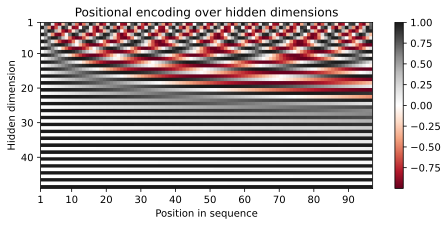
\includegraphics{002_awwe_files/figure-pdf/cell-11-output-1.pdf}

\begin{itemize}
\tightlist
\item
  Let's plot the second example, taper ratio \(\lambda\) and fuel weight
  \(W_{fw}\)
\item
  This is combination \texttt{11}:
\end{itemize}

\begin{Shaded}
\begin{Highlighting}[]
\NormalTok{p }\OperatorTok{=} \DecValTok{11}
\NormalTok{Zlab[p]}
\end{Highlighting}
\end{Shaded}

\begin{verbatim}
['Wfw', 'l']
\end{verbatim}

\begin{Shaded}
\begin{Highlighting}[]
\NormalTok{plt.contourf(X, Y, Z[p], }\DecValTok{20}\NormalTok{, cmap}\OperatorTok{=}\StringTok{\textquotesingle{}jet\textquotesingle{}}\NormalTok{, vmin}\OperatorTok{=}\DecValTok{180}\NormalTok{, vmax}\OperatorTok{=}\DecValTok{360}\NormalTok{)}
\NormalTok{plt.xlabel(Zlab[p][}\DecValTok{0}\NormalTok{])}
\NormalTok{plt.ylabel(Zlab[p][}\DecValTok{1}\NormalTok{])}
\NormalTok{plt.colorbar()}
\end{Highlighting}
\end{Shaded}

\includegraphics{002_awwe_files/figure-pdf/cell-13-output-1.pdf}

\begin{itemize}
\tightlist
\item
  Using a global colormap indicates that these variables have minor
  effects on the wing weight.
\item
  Important factors can be detected by visual inspection
\item
  Plotting the Big Picture: we can plot all 36 combinations in one
  figure.
\end{itemize}

\begin{Shaded}
\begin{Highlighting}[]
\ImportTok{import}\NormalTok{ matplotlib.pyplot }\ImportTok{as}\NormalTok{ plt}
\ImportTok{from}\NormalTok{ mpl\_toolkits.axes\_grid1 }\ImportTok{import}\NormalTok{ ImageGrid}
\ImportTok{import}\NormalTok{ numpy }\ImportTok{as}\NormalTok{ np}

\NormalTok{fig }\OperatorTok{=}\NormalTok{ plt.figure(figsize}\OperatorTok{=}\NormalTok{(}\FloatTok{20.}\NormalTok{, }\FloatTok{20.}\NormalTok{))}
\NormalTok{grid }\OperatorTok{=}\NormalTok{ ImageGrid(fig, }\DecValTok{111}\NormalTok{,  }\CommentTok{\# similar to subplot(111)}
\NormalTok{                 nrows\_ncols}\OperatorTok{=}\NormalTok{(}\DecValTok{6}\NormalTok{,}\DecValTok{6}\NormalTok{),  }\CommentTok{\# creates 2x2 grid of axes}
\NormalTok{                 axes\_pad}\OperatorTok{=}\FloatTok{0.5}\NormalTok{,  }\CommentTok{\# pad between axes in inch.}
\NormalTok{                 share\_all}\OperatorTok{=}\VariableTok{True}\NormalTok{,}
\NormalTok{                 label\_mode}\OperatorTok{=}\StringTok{"0"}\NormalTok{,}
\NormalTok{                 ) }
\NormalTok{i }\OperatorTok{=} \DecValTok{0}
\ControlFlowTok{for}\NormalTok{ ax, im }\KeywordTok{in} \BuiltInTok{zip}\NormalTok{(grid, Z):}
    \CommentTok{\# Iterating over the grid returns the Axes.}
\NormalTok{    ax.set\_xlabel(Zlab[i][}\DecValTok{0}\NormalTok{])}
\NormalTok{    ax.set\_ylabel(Zlab[i][}\DecValTok{1}\NormalTok{])}
    \CommentTok{\# ax.set\_title(Zlab[i][1] + " vs. " + Zlab[i][0])}
\NormalTok{    ax.contourf(X, Y, im, }\DecValTok{30}\NormalTok{, cmap }\OperatorTok{=} \StringTok{"jet"}\NormalTok{,  vmin }\OperatorTok{=} \DecValTok{180}\NormalTok{, vmax }\OperatorTok{=} \DecValTok{360}\NormalTok{)}
\NormalTok{    i }\OperatorTok{=}\NormalTok{ i }\OperatorTok{+} \DecValTok{1}
       
\NormalTok{plt.show()}
\end{Highlighting}
\end{Shaded}

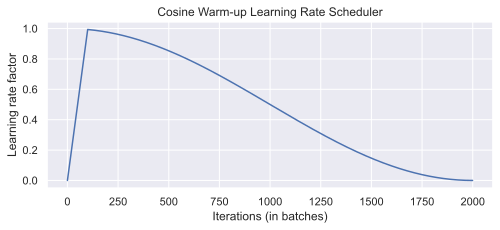
\includegraphics{002_awwe_files/figure-pdf/cell-14-output-1.pdf}

\section{AWWE Landscape}\label{awwe-landscape}

\begin{itemize}
\tightlist
\item
  Our Observations

  \begin{enumerate}
  \def\labelenumi{\arabic{enumi}.}
  \tightlist
  \item
    The load factor \(N_z\), which determines the magnitude of the
    maximum aerodynamic load on the wing, is very active and involved in
    interactions with other variables.
  \end{enumerate}

  \begin{itemize}
  \tightlist
  \item
    Classic example: the interaction of \(N_z\) with the aspect ratio
    \(A\) indicates a heavy wing for high aspect ratios and large
    \(g\)-forces
  \item
    This is the reaon why highly manoeuvrable fighter jets cannot have
    very efficient, glider wings)
  \end{itemize}

  \begin{enumerate}
  \def\labelenumi{\arabic{enumi}.}
  \setcounter{enumi}{1}
  \tightlist
  \item
    Aspect ratio \(A\) and airfoil thickness to chord ratio \(R_{tc}\)
    have nonlinear interactions.
  \item
    Most important variables:
  \end{enumerate}

  \begin{itemize}
  \tightlist
  \item
    Ultimate load factor \(N_z\), wing area \(S_w\), and flight design
    gross weight\(W_{dg}\).
  \end{itemize}

  \begin{enumerate}
  \def\labelenumi{\arabic{enumi}.}
  \setcounter{enumi}{3}
  \tightlist
  \item
    Little impact: dynamic pressure \(q\), taper ratio \(l\), and
    quarter-chord sweep \(L\).
  \end{enumerate}
\item
  Expert Knowledge

  \begin{itemize}
  \tightlist
  \item
    Aircraft designers know that the overall weight of the aircraft and
    the wing area must be kept to a minimum
  \item
    the latter usually dictated by constraints such as required stall
    speed, landing distance, turn rate, etc.
  \end{itemize}
\end{itemize}

\section{Summary of the First
Experiments}\label{summary-of-the-first-experiments}

\begin{itemize}
\tightlist
\item
  First, we considered two pairs of inputs, out of 36 total pairs
\item
  Then, the ``Big Picture'':

  \begin{itemize}
  \tightlist
  \item
    For each pair we evaluated \texttt{wingwt} 10,000 times
  \end{itemize}
\item
  Doing the same for all pairs would require 360K evaluations:

  \begin{itemize}
  \tightlist
  \item
    not a reasonable number with a real computer simulation that takes
    any non-trivial amount of time to evaluate
  \item
    Only 1s per evaluation: \(>100\) hours
  \end{itemize}
\item
  Many solvers take minutes/hours/days to execute a single run
\item
  And: three-way interactions?
\item
  Consequence: a different strategy is needed
\end{itemize}

\section{Exercise}\label{exercise}

\subsection{Adding Paint Weight}\label{adding-paint-weight}

\begin{itemize}
\tightlist
\item
  Paint weight is not considered.
\item
  Add Paint Weight \(W_p\) to formula (the updated formula is shown
  below) and update the functions and plots in the notebook.
\end{itemize}

\[ W = 0.036S_W^{0.758} \times W_{fw}^{0.0035} \times \left( \frac{A}{\cos^2 \Lambda} \right)^{0.6} \times q^{0.006} \times \lambda^{0.04} \]
\[ \times \left( \frac{100 R_{tc}}{\cos \Lambda} \right)^{-0.3} \times (N_z W_{dg})^{0.49} + S_w W_p\]

\section{Jupyter Notebook}\label{jupyter-notebook-1}

\begin{tcolorbox}[enhanced jigsaw, rightrule=.15mm, opacitybacktitle=0.6, coltitle=black, bottomrule=.15mm, bottomtitle=1mm, title=\textcolor{quarto-callout-note-color}{\faInfo}\hspace{0.5em}{Note}, left=2mm, colframe=quarto-callout-note-color-frame, titlerule=0mm, toptitle=1mm, arc=.35mm, colbacktitle=quarto-callout-note-color!10!white, breakable, toprule=.15mm, opacityback=0, leftrule=.75mm, colback=white]

\begin{itemize}
\tightlist
\item
  The Jupyter-Notebook of this lecture is available on GitHub in the
  \href{https://github.com/sequential-parameter-optimization/Hyperparameter-Tuning-Cookbook/blob/main/002_awwe.ipynb}{Hyperparameter-Tuning-Cookbook
  Repository}
\end{itemize}

\end{tcolorbox}

\chapter{\texorpdfstring{Introduction to
\texttt{scipy.optimize}}{Introduction to scipy.optimize}}\label{introduction-to-scipy.optimize}

\href{https://scipy.org}{SciPy} provides algorithms for optimization,
integration, interpolation, eigenvalue problems, algebraic equations,
differential equations, statistics and many other classes of problems.
SciPy is a collection of mathematical algorithms and convenience
functions built on NumPy. It adds significant power to Python by
providing the user with high-level commands and classes for manipulating
and visualizing data.

\href{https://docs.scipy.org/doc/scipy/reference/optimize.html\#module-scipy.optimize}{SciPy
optimize} provides functions for minimizing (or maximizing) objective
functions, possibly subject to constraints. It includes solvers for
nonlinear problems (with support for both local and global optimization
algorithms), linear programing, constrained and nonlinear least-squares,
root finding, and curve fitting.

In this notebook, we will learn how to use the \texttt{scipy.optimize}
module to solve optimization problems. See:
\url{https://docs.scipy.org/doc/scipy/tutorial/optimize.html}

\begin{tcolorbox}[enhanced jigsaw, rightrule=.15mm, opacitybacktitle=0.6, coltitle=black, bottomrule=.15mm, bottomtitle=1mm, title=\textcolor{quarto-callout-note-color}{\faInfo}\hspace{0.5em}{Note}, left=2mm, colframe=quarto-callout-note-color-frame, titlerule=0mm, toptitle=1mm, arc=.35mm, colbacktitle=quarto-callout-note-color!10!white, breakable, toprule=.15mm, opacityback=0, leftrule=.75mm, colback=white]

\begin{itemize}
\tightlist
\item
  This content is based on information from the scipy.optimize package.
\item
  The \texttt{scipy.optimize} package provides several commonly used
  optimization algorithms. A detailed listing is available in
  \texttt{scipy.optimize} (can also be found by
  \texttt{help(scipy.optimize)}).
\end{itemize}

\end{tcolorbox}

Common functions and objects, shared across different SciPy optimize
solvers, are shown in Table~\ref{tbl-shared-functions}.

\begin{longtable}[]{@{}
  >{\raggedright\arraybackslash}p{(\columnwidth - 2\tabcolsep) * \real{0.5000}}
  >{\raggedright\arraybackslash}p{(\columnwidth - 2\tabcolsep) * \real{0.5000}}@{}}
\caption{Common functions and objects, shared across different SciPy
optimize solvers}\label{tbl-shared-functions}\tabularnewline
\toprule\noalign{}
\begin{minipage}[b]{\linewidth}\raggedright
Function or Object
\end{minipage} & \begin{minipage}[b]{\linewidth}\raggedright
Description
\end{minipage} \\
\midrule\noalign{}
\endfirsthead
\toprule\noalign{}
\begin{minipage}[b]{\linewidth}\raggedright
Function or Object
\end{minipage} & \begin{minipage}[b]{\linewidth}\raggedright
Description
\end{minipage} \\
\midrule\noalign{}
\endhead
\bottomrule\noalign{}
\endlastfoot
\href{https://docs.scipy.org/doc/scipy/reference/generated/scipy.optimize.show_options.html\#scipy.optimize.show_options}{show\_options({[}solver,
method, disp{]})} & Show documentation for additional options of
optimization solvers. \\
\href{https://docs.scipy.org/doc/scipy/reference/generated/scipy.optimize.OptimizeResult.html\#scipy.optimize.OptimizeResult}{OptimizeResult}
& Represents the optimization result. \\
\href{https://docs.scipy.org/doc/scipy/reference/generated/scipy.optimize.OptimizeWarning.html\#scipy.optimize.OptimizeWarning}{OptimizeWarning}
& Warning issued by solvers. \\
\end{longtable}

We will introduce unconstrained minimization of multivariate scalar
functions in this chapter. The
\href{https://docs.scipy.org/doc/scipy/reference/generated/scipy.optimize.minimize.html\#scipy.optimize.minimize}{minimize}
function provides a common interface to unconstrained and constrained
minimization algorithms for multivariate scalar functions in
\texttt{scipy.optimize}. To demonstrate the minimization function,
consider the problem of minimizing the Rosenbrock function of \emph{N}
variables:

\[
f(J) = \sum_{i=1}^{N-1} 100 (x_{i+1} - x_i^2)^2 + (1 - x_i)^2
\]

The minimum value of this function is 0, which is achieved when (x\_i =
1).

Note that the Rosenbrock function and its derivatives are included in
\texttt{scipy.optimize}. The implementations shown in the following
sections provide examples of how to define an objective function as well
as its Jacobian and Hessian functions. Objective functions in
\texttt{scipy.optimize} expect a numpy array as their first parameter,
which is to be optimized and must return a float value. The exact
calling signature must be \texttt{f(x,\ *args)}, where \texttt{x}
represents a numpy array, and \texttt{args} is a tuple of additional
arguments supplied to the objective function.

\section{Derivative-free Optimization
Algorithms}\label{derivative-free-optimization-algorithms}

Section~\ref{sec-nelder-mead-simplex-algorithm} and
Section~\ref{sec-powells-method} present two approaches that do not need
gradient information to find the minimum. They use function evaluations
to find the minimum.

\subsection{Nelder-Mead Simplex
Algorithm}\label{sec-nelder-mead-simplex-algorithm}

\texttt{method=\textquotesingle{}Nelder-Mead\textquotesingle{}}: In the
example below, the \texttt{minimize} routine is used with the
\emph{Nelder-Mead} simplex algorithm (selected through the
\texttt{method} parameter):

\begin{Shaded}
\begin{Highlighting}[]
\ImportTok{import}\NormalTok{ numpy }\ImportTok{as}\NormalTok{ np}
\ImportTok{from}\NormalTok{ scipy.optimize }\ImportTok{import}\NormalTok{ minimize}

\KeywordTok{def}\NormalTok{ rosen(x):}
    \CommentTok{"""The Rosenbrock function"""}
    \ControlFlowTok{return} \BuiltInTok{sum}\NormalTok{(}\FloatTok{100.0} \OperatorTok{*}\NormalTok{ (x[}\DecValTok{1}\NormalTok{:] }\OperatorTok{{-}}\NormalTok{ x[:}\OperatorTok{{-}}\DecValTok{1}\NormalTok{]}\OperatorTok{**}\FloatTok{2.0}\NormalTok{)}\OperatorTok{**}\FloatTok{2.0} \OperatorTok{+}\NormalTok{ (}\DecValTok{1} \OperatorTok{{-}}\NormalTok{ x[:}\OperatorTok{{-}}\DecValTok{1}\NormalTok{])}\OperatorTok{**}\FloatTok{2.0}\NormalTok{)}

\NormalTok{x0 }\OperatorTok{=}\NormalTok{ np.array([}\FloatTok{1.3}\NormalTok{, }\FloatTok{0.7}\NormalTok{, }\FloatTok{0.8}\NormalTok{, }\FloatTok{1.9}\NormalTok{, }\FloatTok{1.2}\NormalTok{])}
\NormalTok{res }\OperatorTok{=}\NormalTok{ minimize(rosen, x0, method}\OperatorTok{=}\StringTok{\textquotesingle{}nelder{-}mead\textquotesingle{}}\NormalTok{,}
\NormalTok{               options}\OperatorTok{=}\NormalTok{\{}\StringTok{\textquotesingle{}xatol\textquotesingle{}}\NormalTok{: }\FloatTok{1e{-}8}\NormalTok{, }\StringTok{\textquotesingle{}disp\textquotesingle{}}\NormalTok{: }\VariableTok{True}\NormalTok{\})}

\BuiltInTok{print}\NormalTok{(res.x)}
\end{Highlighting}
\end{Shaded}

\begin{verbatim}
Optimization terminated successfully.
         Current function value: 0.000000
         Iterations: 339
         Function evaluations: 571
[1. 1. 1. 1. 1.]
\end{verbatim}

The simplex algorithm is probably the simplest way to minimize a
well-behaved function. It requires only function evaluations and is a
good choice for simple minimization problems. However, because it does
not use any gradient evaluations, it may take longer to find the
minimum.

\subsection{Powell's Method}\label{sec-powells-method}

Another optimization algorithm that needs only function calls to find
the minimum is \emph{Powell}'s method, which can be selected by setting
the \texttt{method} parameter to
\texttt{\textquotesingle{}powell\textquotesingle{}} in the
\texttt{minimize} function.

To demonstrate how to supply additional arguments to an objective
function, let's consider minimizing the Rosenbrock function with an
additional scaling factor \(a\) and an offset \(b\):

\[
f(J, a, b) = \sum_{i=1}^{N-1} a (x_{i+1} - x_i^2)^2 + (1 - x_i)^2 + b
\]

You can achieve this using the \texttt{minimize} routine with the
example parameters \(a=0.5\) and \(b=1\):

\begin{Shaded}
\begin{Highlighting}[]
\KeywordTok{def}\NormalTok{ rosen\_with\_args(x, a, b):}
    \CommentTok{"""The Rosenbrock function with additional arguments"""}
    \ControlFlowTok{return} \BuiltInTok{sum}\NormalTok{(a }\OperatorTok{*}\NormalTok{ (x[}\DecValTok{1}\NormalTok{:] }\OperatorTok{{-}}\NormalTok{ x[:}\OperatorTok{{-}}\DecValTok{1}\NormalTok{]}\OperatorTok{**}\FloatTok{2.0}\NormalTok{)}\OperatorTok{**}\FloatTok{2.0} \OperatorTok{+}\NormalTok{ (}\DecValTok{1} \OperatorTok{{-}}\NormalTok{ x[:}\OperatorTok{{-}}\DecValTok{1}\NormalTok{])}\OperatorTok{**}\FloatTok{2.0}\NormalTok{) }\OperatorTok{+}\NormalTok{ b}

\NormalTok{x0 }\OperatorTok{=}\NormalTok{ np.array([}\FloatTok{1.3}\NormalTok{, }\FloatTok{0.7}\NormalTok{, }\FloatTok{0.8}\NormalTok{, }\FloatTok{1.9}\NormalTok{, }\FloatTok{1.2}\NormalTok{])}
\NormalTok{res }\OperatorTok{=}\NormalTok{ minimize(rosen\_with\_args, x0, method}\OperatorTok{=}\StringTok{\textquotesingle{}nelder{-}mead\textquotesingle{}}\NormalTok{,}
\NormalTok{               args}\OperatorTok{=}\NormalTok{(}\FloatTok{0.5}\NormalTok{, }\FloatTok{1.}\NormalTok{), options}\OperatorTok{=}\NormalTok{\{}\StringTok{\textquotesingle{}xatol\textquotesingle{}}\NormalTok{: }\FloatTok{1e{-}8}\NormalTok{, }\StringTok{\textquotesingle{}disp\textquotesingle{}}\NormalTok{: }\VariableTok{True}\NormalTok{\})}

\BuiltInTok{print}\NormalTok{(res.x)}
\end{Highlighting}
\end{Shaded}

\begin{verbatim}
Optimization terminated successfully.
         Current function value: 1.000000
         Iterations: 319
         Function evaluations: 525
[1.         1.         1.         1.         0.99999999]
\end{verbatim}

As an alternative to using the \texttt{args} parameter of
\texttt{minimize}, you can wrap the objective function in a new function
that accepts only \texttt{x}. This approach is also useful when it is
necessary to pass additional parameters to the objective function as
keyword arguments.

\begin{Shaded}
\begin{Highlighting}[]
\KeywordTok{def}\NormalTok{ rosen\_with\_args(x, a, }\OperatorTok{*}\NormalTok{, b):  }\CommentTok{\# b is a keyword{-}only argument}
    \ControlFlowTok{return} \BuiltInTok{sum}\NormalTok{(a }\OperatorTok{*}\NormalTok{ (x[}\DecValTok{1}\NormalTok{:] }\OperatorTok{{-}}\NormalTok{ x[:}\OperatorTok{{-}}\DecValTok{1}\NormalTok{]}\OperatorTok{**}\FloatTok{2.0}\NormalTok{)}\OperatorTok{**}\FloatTok{2.0} \OperatorTok{+}\NormalTok{ (}\DecValTok{1} \OperatorTok{{-}}\NormalTok{ x[:}\OperatorTok{{-}}\DecValTok{1}\NormalTok{])}\OperatorTok{**}\FloatTok{2.0}\NormalTok{) }\OperatorTok{+}\NormalTok{ b}

\KeywordTok{def}\NormalTok{ wrapped\_rosen\_without\_args(x):}
    \ControlFlowTok{return}\NormalTok{ rosen\_with\_args(x, }\FloatTok{0.5}\NormalTok{, b}\OperatorTok{=}\FloatTok{1.}\NormalTok{)  }\CommentTok{\# pass in \textasciigrave{}a\textasciigrave{} and \textasciigrave{}b\textasciigrave{}}

\NormalTok{x0 }\OperatorTok{=}\NormalTok{ np.array([}\FloatTok{1.3}\NormalTok{, }\FloatTok{0.7}\NormalTok{, }\FloatTok{0.8}\NormalTok{, }\FloatTok{1.9}\NormalTok{, }\FloatTok{1.2}\NormalTok{])}
\NormalTok{res }\OperatorTok{=}\NormalTok{ minimize(wrapped\_rosen\_without\_args, x0, method}\OperatorTok{=}\StringTok{\textquotesingle{}nelder{-}mead\textquotesingle{}}\NormalTok{,}
\NormalTok{               options}\OperatorTok{=}\NormalTok{\{}\StringTok{\textquotesingle{}xatol\textquotesingle{}}\NormalTok{: }\FloatTok{1e{-}8}\NormalTok{,\})}

\BuiltInTok{print}\NormalTok{(res.x)}
\end{Highlighting}
\end{Shaded}

\begin{verbatim}
[1.         1.         1.         1.         0.99999999]
\end{verbatim}

Another alternative is to use \texttt{functools.partial}.

\begin{Shaded}
\begin{Highlighting}[]
\ImportTok{from}\NormalTok{ functools }\ImportTok{import}\NormalTok{ partial}

\NormalTok{partial\_rosen }\OperatorTok{=}\NormalTok{ partial(rosen\_with\_args, a}\OperatorTok{=}\FloatTok{0.5}\NormalTok{, b}\OperatorTok{=}\FloatTok{1.}\NormalTok{)}
\NormalTok{res }\OperatorTok{=}\NormalTok{ minimize(partial\_rosen, x0, method}\OperatorTok{=}\StringTok{\textquotesingle{}nelder{-}mead\textquotesingle{}}\NormalTok{,}
\NormalTok{               options}\OperatorTok{=}\NormalTok{\{}\StringTok{\textquotesingle{}xatol\textquotesingle{}}\NormalTok{: }\FloatTok{1e{-}8}\NormalTok{,\})}

\BuiltInTok{print}\NormalTok{(res.x)}
\end{Highlighting}
\end{Shaded}

\begin{verbatim}
[1.         1.         1.         1.         0.99999999]
\end{verbatim}

\section{Gradient-based optimization
algorithms}\label{gradient-based-optimization-algorithms}

\subsection{An Introductory Example: Broyden-Fletcher-Goldfarb-Shanno
Algorithm (BFGS)}\label{sec-bfgs-intro}

This section introduces an optimization algorithm that uses gradient
information to find the minimum. The Broyden-Fletcher-Goldfarb-Shanno
(BFGS) algorithm (selected by setting
\texttt{method=\textquotesingle{}BFGS\textquotesingle{}}) is an
optimization algorithm that aims to converge quickly to the solution.
This algorithm uses the gradient of the objective function. If the
gradient is not provided by the user, it is estimated using
first-differences. The BFGS method typically requires fewer function
calls compared to the simplex algorithm, even when the gradient needs to
be estimated.

\begin{tcolorbox}[enhanced jigsaw, rightrule=.15mm, opacitybacktitle=0.6, coltitle=black, bottomrule=.15mm, bottomtitle=1mm, title=\textcolor{quarto-callout-note-color}{\faInfo}\hspace{0.5em}{Example: BFGS}, left=2mm, colframe=quarto-callout-note-color-frame, titlerule=0mm, toptitle=1mm, arc=.35mm, colbacktitle=quarto-callout-note-color!10!white, breakable, toprule=.15mm, opacityback=0, leftrule=.75mm, colback=white]

To demonstrate the BFGS algorithm, let's use the Rosenbrock function
again. The gradient of the Rosenbrock function is a vector described by
the following mathematical expression:

\begin{align}
\frac{\partial f}{\partial x_j} = \sum_{i=1}^{N} 200(x_i - x_{i-1}^2)(\delta_{i,j} - 2x_{i-1}\delta_{i-1,j}) - 2(1 - x_{i-1})\delta_{i-1,j} \\
= 200(x_j - x_{j-1}^2) - 400x_j(x_{j+1} - x_j^2) - 2(1 - x_j)
\end{align}

This expression is valid for interior derivatives, but special cases
are:

\[
\frac{\partial f}{\partial x_0} = -400x_0(x_1 - x_0^2) - 2(1 - x_0)
\]

\[
\frac{\partial f}{\partial x_{N-1}} = 200(x_{N-1} - x_{N-2}^2)
\]

Here's a Python function that computes this gradient:

\begin{Shaded}
\begin{Highlighting}[]
\KeywordTok{def}\NormalTok{ rosen\_der(x):}
\NormalTok{    xm }\OperatorTok{=}\NormalTok{ x[}\DecValTok{1}\NormalTok{:}\OperatorTok{{-}}\DecValTok{1}\NormalTok{]}
\NormalTok{    xm\_m1 }\OperatorTok{=}\NormalTok{ x[:}\OperatorTok{{-}}\DecValTok{2}\NormalTok{]}
\NormalTok{    xm\_p1 }\OperatorTok{=}\NormalTok{ x[}\DecValTok{2}\NormalTok{:]}
\NormalTok{    der }\OperatorTok{=}\NormalTok{ np.zeros\_like(x)}
\NormalTok{    der[}\DecValTok{1}\NormalTok{:}\OperatorTok{{-}}\DecValTok{1}\NormalTok{] }\OperatorTok{=} \DecValTok{200}\OperatorTok{*}\NormalTok{(xm}\OperatorTok{{-}}\NormalTok{xm\_m1}\OperatorTok{**}\DecValTok{2}\NormalTok{) }\OperatorTok{{-}} \DecValTok{400}\OperatorTok{*}\NormalTok{(xm\_p1 }\OperatorTok{{-}}\NormalTok{ xm}\OperatorTok{**}\DecValTok{2}\NormalTok{)}\OperatorTok{*}\NormalTok{xm }\OperatorTok{{-}} \DecValTok{2}\OperatorTok{*}\NormalTok{(}\DecValTok{1}\OperatorTok{{-}}\NormalTok{xm)}
\NormalTok{    der[}\DecValTok{0}\NormalTok{] }\OperatorTok{=} \OperatorTok{{-}}\DecValTok{400}\OperatorTok{*}\NormalTok{x[}\DecValTok{0}\NormalTok{]}\OperatorTok{*}\NormalTok{(x[}\DecValTok{1}\NormalTok{]}\OperatorTok{{-}}\NormalTok{x[}\DecValTok{0}\NormalTok{]}\OperatorTok{**}\DecValTok{2}\NormalTok{) }\OperatorTok{{-}} \DecValTok{2}\OperatorTok{*}\NormalTok{(}\DecValTok{1}\OperatorTok{{-}}\NormalTok{x[}\DecValTok{0}\NormalTok{])}
\NormalTok{    der[}\OperatorTok{{-}}\DecValTok{1}\NormalTok{] }\OperatorTok{=} \DecValTok{200}\OperatorTok{*}\NormalTok{(x[}\OperatorTok{{-}}\DecValTok{1}\NormalTok{]}\OperatorTok{{-}}\NormalTok{x[}\OperatorTok{{-}}\DecValTok{2}\NormalTok{]}\OperatorTok{**}\DecValTok{2}\NormalTok{)}
    \ControlFlowTok{return}\NormalTok{ der}
\end{Highlighting}
\end{Shaded}

You can specify this gradient information in the minimize function using
the jac parameter as illustrated below:

\begin{Shaded}
\begin{Highlighting}[]
\NormalTok{res }\OperatorTok{=}\NormalTok{ minimize(rosen, x0, method}\OperatorTok{=}\StringTok{\textquotesingle{}BFGS\textquotesingle{}}\NormalTok{, jac}\OperatorTok{=}\NormalTok{rosen\_der,}
\NormalTok{               options}\OperatorTok{=}\NormalTok{\{}\StringTok{\textquotesingle{}disp\textquotesingle{}}\NormalTok{: }\VariableTok{True}\NormalTok{\})}

\BuiltInTok{print}\NormalTok{(res.x)}
\end{Highlighting}
\end{Shaded}

\begin{verbatim}
Optimization terminated successfully.
         Current function value: 0.000000
         Iterations: 25
         Function evaluations: 30
         Gradient evaluations: 30
[1.00000004 1.0000001  1.00000021 1.00000044 1.00000092]
\end{verbatim}

\end{tcolorbox}

\subsection{Background and Basics for Gradient-based
Optimization}\label{background-and-basics-for-gradient-based-optimization}

\subsection{Gradient}\label{gradient}

The gradient \(\nabla f(J)\) for a scalar function \(f(J)\) with \(n\)
different variables is defined by its partial derivatives:

\[\nabla f(J) = \left[ \frac{\partial f}{\partial x_1}, \frac{\partial f}{\partial x_2}, \ldots, \frac{\partial f}{\partial x_n} \right]\]

\subsection{Jacobian Matrix}\label{jacobian-matrix}

The Jacobian matrix \(J(J)\) for a vector-valued function
\(F(J) = [f_1(J), f_2(J), \ldots, f_m(J)]\) is defined as:

\(J(J) = \begin{bmatrix} \frac{\partial f_1}{\partial x_1} & \frac{\partial f_1}{\partial x_2} & \ldots & \frac{\partial f_1}{\partial x_n} \\ \frac{\partial f_2}{\partial x_1} & \frac{\partial f_2}{\partial x_2} & \ldots & \frac{\partial f_2}{\partial x_n} \\ \vdots & \vdots & \ddots & \vdots \\ \frac{\partial f_m}{\partial x_1} & \frac{\partial f_m}{\partial x_2} & \ldots & \frac{\partial f_m}{\partial x_n} \end{bmatrix}\)

It consists of the first order partial derivatives and gives therefore
an overview about the gradients of a vector valued function.

\begin{tcolorbox}[enhanced jigsaw, rightrule=.15mm, opacitybacktitle=0.6, coltitle=black, bottomrule=.15mm, bottomtitle=1mm, title=\textcolor{quarto-callout-note-color}{\faInfo}\hspace{0.5em}{Example: Jacobian matrix}, left=2mm, colframe=quarto-callout-note-color-frame, titlerule=0mm, toptitle=1mm, arc=.35mm, colbacktitle=quarto-callout-note-color!10!white, breakable, toprule=.15mm, opacityback=0, leftrule=.75mm, colback=white]

Consider a vector-valued function
\(f : \mathbb{R}^2 \rightarrow \mathbb{R}^3\) defined as follows:
\[f(J) = \begin{bmatrix} x_1^2 + 2x_2 \\ 3x_1 - \sin(x_2) \\ e^{x_1 + x_2} \end{bmatrix}\]

Let's compute the partial derivatives and construct the Jacobian matrix:

\(\frac{\partial f_1}{\partial x_1} = 2x_1, \quad \frac{\partial f_1}{\partial x_2} = 2\)

\(\frac{\partial f_2}{\partial x_1} = 3, \quad \frac{\partial f_2}{\partial x_2} = -\cos(x_2)\)

\(\frac{\partial f_3}{\partial x_1} = e^{x_1 + x_2}, \quad \frac{\partial f_3}{\partial x_2} = e^{x_1 + x_2}\)

So, the Jacobian matrix is:

\[J(J) = \begin{bmatrix} 2x_1 & 2 \\ 3 & -\cos(x_2) \\ e^{x_1 + x_2} & e^{x_1 + x_2} \end{bmatrix}\]

This Jacobian matrix provides information about how small changes in the
input variables \(x_1\) and \(x_2\) affect the corresponding changes in
each component of the output vector.

\end{tcolorbox}

\subsection{Hessian Matrix}\label{hessian-matrix}

The Hessian matrix \(H(J)\) for a scalar function \(f(J)\) is defined
as:

\(H(J) = \begin{bmatrix} \frac{\partial^2 f}{\partial x_1^2} & \frac{\partial^2 f}{\partial x_1 \partial x_2} & \ldots & \frac{\partial^2 f}{\partial x_1 \partial x_n} \\ \frac{\partial^2 f}{\partial x_2 \partial x_1} & \frac{\partial^2 f}{\partial x_2^2} & \ldots & \frac{\partial^2 f}{\partial x_2 \partial x_n} \\ \vdots & \vdots & \ddots & \vdots \\ \frac{\partial^2 f}{\partial x_n \partial x_1} & \frac{\partial^2 f}{\partial x_n \partial x_2} & \ldots & \frac{\partial^2 f}{\partial x_n^2} \end{bmatrix}\)

So, the Hessian matrix consists of the second order dervatives of the
function. It provides information about the local curvature of the
function with respect to changes in the input variables.

\begin{tcolorbox}[enhanced jigsaw, rightrule=.15mm, opacitybacktitle=0.6, coltitle=black, bottomrule=.15mm, bottomtitle=1mm, title=\textcolor{quarto-callout-note-color}{\faInfo}\hspace{0.5em}{Example: Hessian matrix}, left=2mm, colframe=quarto-callout-note-color-frame, titlerule=0mm, toptitle=1mm, arc=.35mm, colbacktitle=quarto-callout-note-color!10!white, breakable, toprule=.15mm, opacityback=0, leftrule=.75mm, colback=white]

Consider a scalar-valued function:
\[f(J) = x_1^2 + 2x_2^2 + \sin(x_1   x_2)\]

The Hessian matrix of this scalar-valued function is the matrix of its
second-order partial derivatives with respect to the input variables:
\[H(J) = \begin{bmatrix} \frac{\partial^2 f}{\partial x_1^2} & \frac{\partial^2 f}{\partial x_1 \partial x_2} \\ \frac{\partial^2 f}{\partial x_2 \partial x_1} & \frac{\partial^2 f}{\partial x_2^2} \end{bmatrix}\]

Let's compute the second-order partial derivatives and construct the
Hessian matrix:

\begin{align}
\frac{\partial^2 f}{\partial x_1^2} &= 2 + \cos(x_1 x_2) x_2^2\\
\frac{\partial^2 f}{\partial x_1 \partial x_2} &= 2x_1  x_2 \cos(x_1 x_2) - \sin(x_1  x_2)\\
\frac{\partial^2 f}{\partial x_2 \partial x_1} &= 2x_1  x_2  \cos(x_1  x_2) - \sin(x_1  x_2)\\
\frac{\partial^2 f}{\partial x_2^2} &= 4x_2^2 + \cos(x_1  x_2) x_1^2
\end{align}

So, the Hessian matrix is:

\[H(J) = \begin{bmatrix} 2 + \cos(x_1   x_2)   x_2^2 & 2x_1   x_2   \cos(x_1   x_2) - \sin(x_1   x_2) \\ 2x_1   x_2   \cos(x_1   x_2) - \sin(x_1   x_2) & 4x_2^2 + \cos(x_1   x_2)   x_1^2 \end{bmatrix}\]

\end{tcolorbox}

\subsection{Gradient for Optimization}\label{gradient-for-optimization}

In optimization, the goal is to find the minimum or maximum of a
function. Gradient-based optimization methods utilize information about
the gradient (or derivative) of the function to guide the search for the
optimal solution. This is particularly useful when dealing with complex,
high-dimensional functions where an exhaustive search is impractical.

The gradient descent method can be divided in the following steps:

\begin{itemize}
\tightlist
\item
  \textbf{Initialize:} start with an initial guess for the parameters of
  the function to be optimized.
\item
  \textbf{Compute Gradient:} Calculate the gradient (partial
  derivatives) of the function with respect to each parameter at the
  current point. The gradient indicates the direction of the steepest
  increase in the function.
\item
  \textbf{Update Parameters:} Adjust the parameters in the opposite
  direction of the gradient, scaled by a learning rate. This step aims
  to move towards the minimum of the function:

  \begin{itemize}
  \tightlist
  \item
    \(x_{k+1} = x_k - \alpha \times \nabla f(x_{k})\)
  \item
    \(x_{x}\) is current parameter vector or point in the parameter
    space.
  \item
    \(\alpha\) is the learning rate, a positive scalar that determines
    the step size in each iteration.
  \item
    \(\nabla f(x)\) is the gradient of the objective function.
  \end{itemize}
\item
  \textbf{Iterate:} Repeat the above steps until convergence or a
  predefined number of iterations. Convergence is typically determined
  when the change in the function value or parameters becomes
  negligible.
\end{itemize}

\begin{tcolorbox}[enhanced jigsaw, rightrule=.15mm, opacitybacktitle=0.6, coltitle=black, bottomrule=.15mm, bottomtitle=1mm, title=\textcolor{quarto-callout-note-color}{\faInfo}\hspace{0.5em}{Example: Gradient Descent}, left=2mm, colframe=quarto-callout-note-color-frame, titlerule=0mm, toptitle=1mm, arc=.35mm, colbacktitle=quarto-callout-note-color!10!white, breakable, toprule=.15mm, opacityback=0, leftrule=.75mm, colback=white]

Let's consider a simple quadratic function as an example:
\[f(x) = x^2 + 4x + y^2 + 2y + 4.\]

We'll use gradient descent to find the minimum of this function.

\begin{Shaded}
\begin{Highlighting}[]
\ImportTok{import}\NormalTok{ numpy }\ImportTok{as}\NormalTok{ np}
\ImportTok{import}\NormalTok{ matplotlib.pyplot }\ImportTok{as}\NormalTok{ plt}
\ImportTok{from}\NormalTok{ mpl\_toolkits.mplot3d }\ImportTok{import}\NormalTok{ Axes3D}

\CommentTok{\# Define the quadratic function}
\KeywordTok{def}\NormalTok{ quadratic\_function(x, y):}
    \ControlFlowTok{return}\NormalTok{ x}\OperatorTok{**}\DecValTok{2} \OperatorTok{+} \DecValTok{4}\OperatorTok{*}\NormalTok{x }\OperatorTok{+}\NormalTok{ y}\OperatorTok{**}\DecValTok{2} \OperatorTok{+} \DecValTok{2}\OperatorTok{*}\NormalTok{y }\OperatorTok{+} \DecValTok{4}

\CommentTok{\# Define the gradient of the quadratic function}
\KeywordTok{def}\NormalTok{ gradient\_quadratic\_function(x, y):}
\NormalTok{    grad\_x }\OperatorTok{=} \DecValTok{2}\OperatorTok{*}\NormalTok{x }\OperatorTok{+} \DecValTok{4}
\NormalTok{    grad\_y }\OperatorTok{=} \DecValTok{2}\OperatorTok{*}\NormalTok{y }\OperatorTok{+} \DecValTok{2}
    \ControlFlowTok{return}\NormalTok{ np.array([grad\_x, grad\_y])}

\CommentTok{\# Gradient Descent for optimization in 2D}
\KeywordTok{def}\NormalTok{ gradient\_descent(initial\_point, learning\_rate, num\_iterations):}
\NormalTok{    points }\OperatorTok{=}\NormalTok{ [np.array(initial\_point)]}
    
    \ControlFlowTok{for}\NormalTok{ \_ }\KeywordTok{in} \BuiltInTok{range}\NormalTok{(num\_iterations):}
\NormalTok{        current\_point }\OperatorTok{=}\NormalTok{ points[}\OperatorTok{{-}}\DecValTok{1}\NormalTok{]}
\NormalTok{        gradient }\OperatorTok{=}\NormalTok{ gradient\_quadratic\_function(}\OperatorTok{*}\NormalTok{current\_point)}
\NormalTok{        new\_point }\OperatorTok{=}\NormalTok{ current\_point }\OperatorTok{{-}}\NormalTok{ learning\_rate }\OperatorTok{*}\NormalTok{ gradient}
        
\NormalTok{        points.append(new\_point)}
        
    \ControlFlowTok{return}\NormalTok{ points}

\CommentTok{\# Visualization of optimization process with 3D surface and consistent arrow sizes}
\KeywordTok{def}\NormalTok{ plot\_optimization\_process\_3d\_consistent\_arrows(points):}
\NormalTok{    fig }\OperatorTok{=}\NormalTok{ plt.figure(figsize}\OperatorTok{=}\NormalTok{(}\DecValTok{10}\NormalTok{, }\DecValTok{8}\NormalTok{))}
\NormalTok{    ax }\OperatorTok{=}\NormalTok{ fig.add\_subplot(}\DecValTok{111}\NormalTok{, projection}\OperatorTok{=}\StringTok{\textquotesingle{}3d\textquotesingle{}}\NormalTok{)}

\NormalTok{    x\_vals }\OperatorTok{=}\NormalTok{ np.linspace(}\OperatorTok{{-}}\DecValTok{10}\NormalTok{, }\DecValTok{2}\NormalTok{, }\DecValTok{100}\NormalTok{)}
\NormalTok{    y\_vals }\OperatorTok{=}\NormalTok{ np.linspace(}\OperatorTok{{-}}\DecValTok{10}\NormalTok{, }\DecValTok{2}\NormalTok{, }\DecValTok{100}\NormalTok{)}
\NormalTok{    X, Y }\OperatorTok{=}\NormalTok{ np.meshgrid(x\_vals, y\_vals)}
\NormalTok{    Z }\OperatorTok{=}\NormalTok{ quadratic\_function(X, Y)}

\NormalTok{    ax.plot\_surface(X, Y, Z, cmap}\OperatorTok{=}\StringTok{\textquotesingle{}viridis\textquotesingle{}}\NormalTok{, alpha}\OperatorTok{=}\FloatTok{0.6}\NormalTok{)}
\NormalTok{    ax.scatter(}\OperatorTok{*}\BuiltInTok{zip}\NormalTok{(}\OperatorTok{*}\NormalTok{points), [quadratic\_function(}\OperatorTok{*}\NormalTok{p) }\ControlFlowTok{for}\NormalTok{ p }\KeywordTok{in}\NormalTok{ points], c}\OperatorTok{=}\StringTok{\textquotesingle{}red\textquotesingle{}}\NormalTok{, label}\OperatorTok{=}\StringTok{\textquotesingle{}Optimization Trajectory\textquotesingle{}}\NormalTok{)}

    \ControlFlowTok{for}\NormalTok{ i }\KeywordTok{in} \BuiltInTok{range}\NormalTok{(}\BuiltInTok{len}\NormalTok{(points) }\OperatorTok{{-}} \DecValTok{1}\NormalTok{):  }
\NormalTok{        x, y }\OperatorTok{=}\NormalTok{ points[i]}
\NormalTok{        dx, dy }\OperatorTok{=}\NormalTok{ points[i }\OperatorTok{+} \DecValTok{1}\NormalTok{] }\OperatorTok{{-}}\NormalTok{ points[i]}
\NormalTok{        dz }\OperatorTok{=}\NormalTok{ quadratic\_function(}\OperatorTok{*}\NormalTok{(points[i }\OperatorTok{+} \DecValTok{1}\NormalTok{])) }\OperatorTok{{-}}\NormalTok{ quadratic\_function(}\OperatorTok{*}\NormalTok{points[i])}
\NormalTok{        gradient\_length }\OperatorTok{=} \FloatTok{0.5}

\NormalTok{        ax.quiver(x, y, quadratic\_function(}\OperatorTok{*}\NormalTok{points[i]), dx, dy, dz, color}\OperatorTok{=}\StringTok{\textquotesingle{}blue\textquotesingle{}}\NormalTok{, length}\OperatorTok{=}\NormalTok{gradient\_length, normalize}\OperatorTok{=}\VariableTok{False}\NormalTok{, arrow\_length\_ratio}\OperatorTok{=}\FloatTok{0.1}\NormalTok{)}

\NormalTok{    ax.set\_title(}\StringTok{\textquotesingle{}Gradient{-}Based Optimization with 2D Quadratic Function\textquotesingle{}}\NormalTok{)}
\NormalTok{    ax.set\_xlabel(}\StringTok{\textquotesingle{}x\textquotesingle{}}\NormalTok{)}
\NormalTok{    ax.set\_ylabel(}\StringTok{\textquotesingle{}y\textquotesingle{}}\NormalTok{)}
\NormalTok{    ax.set\_zlabel(}\StringTok{\textquotesingle{}f(x, y)\textquotesingle{}}\NormalTok{)}
\NormalTok{    ax.legend()}
\NormalTok{    plt.show()}

\CommentTok{\# Initial guess and parameters}
\NormalTok{initial\_guess }\OperatorTok{=}\NormalTok{ [}\OperatorTok{{-}}\FloatTok{9.0}\NormalTok{, }\OperatorTok{{-}}\FloatTok{9.0}\NormalTok{]}
\NormalTok{learning\_rate }\OperatorTok{=} \FloatTok{0.2}
\NormalTok{num\_iterations }\OperatorTok{=} \DecValTok{10}

\CommentTok{\# Run gradient descent in 2D and visualize the optimization process with 3D surface and consistent arrow sizes}
\NormalTok{trajectory }\OperatorTok{=}\NormalTok{ gradient\_descent(initial\_guess, learning\_rate, num\_iterations)}
\NormalTok{plot\_optimization\_process\_3d\_consistent\_arrows(trajectory)}
\end{Highlighting}
\end{Shaded}

\includegraphics{003_scipy_optimize_intro_files/figure-pdf/cell-8-output-1.pdf}

\end{tcolorbox}

\subsection{Newton Method}\label{newton-method}

\textbf{Initialization:} Start with an initial guess for the optimal
solution: \(x_0\).

\textbf{Iteration:} Repeat the following three steps until convergence
or a predefined stopping criterion is met:

\begin{enumerate}
\def\labelenumi{\arabic{enumi})}
\item
  Calculate the gradient (\(\nabla\)) and the Hessian matrix
  (\(\nabla^2\)) of the objective function at the current point:
  \[\nabla f(x_k) \quad \text{and} \quad \nabla^2 f(x_k)\]
\item
  Update the current solution using the Newton-Raphson update formula
  \[x_{k+1} = x_k - [\nabla^2 f(x_k)]^{-1} \nabla f(x_k),\] where
\end{enumerate}

\begin{itemize}
\tightlist
\item
  \(\nabla f(x_k)\) is the gradient (first derivative) of the objective
  function with respect to the variable \(x\), evaluated at the current
  solution \(x_k\).
\item
  \(\nabla^2 f(x_k)\): The Hessian matrix (second derivative) of the
  objective function with respect to \(x\), evaluated at the current
  solution \(x_k\).
\item
  \(x_k\): The current solution or point in the optimization process.
\item
  \(\nabla^2 f(x_k)]^{-1}\): The inverse of the Hessian matrix at the
  current point, representing the approximation of the curvature of the
  objective function.
\item
  \(x_{k+1}\): The updated solution or point after applying the
  Newton-Raphson update.
\end{itemize}

\begin{enumerate}
\def\labelenumi{\arabic{enumi})}
\setcounter{enumi}{2}
\tightlist
\item
  Check for convergence.
\end{enumerate}

\begin{tcolorbox}[enhanced jigsaw, rightrule=.15mm, opacitybacktitle=0.6, coltitle=black, bottomrule=.15mm, bottomtitle=1mm, title=\textcolor{quarto-callout-note-color}{\faInfo}\hspace{0.5em}{Example: Newton Method}, left=2mm, colframe=quarto-callout-note-color-frame, titlerule=0mm, toptitle=1mm, arc=.35mm, colbacktitle=quarto-callout-note-color!10!white, breakable, toprule=.15mm, opacityback=0, leftrule=.75mm, colback=white]

We want to optimize the Rosenbrock function and use the Hessian and the
Jacobian (which is equal to the gradient vector for scalar objective
function) to the \texttt{minimize} function.

\begin{Shaded}
\begin{Highlighting}[]
\KeywordTok{def}\NormalTok{ rosenbrock(x):}
    \ControlFlowTok{return} \DecValTok{100} \OperatorTok{*}\NormalTok{ (x[}\DecValTok{1}\NormalTok{] }\OperatorTok{{-}}\NormalTok{ x[}\DecValTok{0}\NormalTok{]}\OperatorTok{**}\DecValTok{2}\NormalTok{)}\OperatorTok{**}\DecValTok{2} \OperatorTok{+}\NormalTok{ (}\DecValTok{1} \OperatorTok{{-}}\NormalTok{ x[}\DecValTok{0}\NormalTok{])}\OperatorTok{**}\DecValTok{2}

\KeywordTok{def}\NormalTok{ rosenbrock\_gradient(x):}
\NormalTok{    dfdx0 }\OperatorTok{=} \OperatorTok{{-}}\DecValTok{400} \OperatorTok{*}\NormalTok{ x[}\DecValTok{0}\NormalTok{] }\OperatorTok{*}\NormalTok{ (x[}\DecValTok{1}\NormalTok{] }\OperatorTok{{-}}\NormalTok{ x[}\DecValTok{0}\NormalTok{]}\OperatorTok{**}\DecValTok{2}\NormalTok{) }\OperatorTok{{-}} \DecValTok{2} \OperatorTok{*}\NormalTok{ (}\DecValTok{1} \OperatorTok{{-}}\NormalTok{ x[}\DecValTok{0}\NormalTok{])}
\NormalTok{    dfdx1 }\OperatorTok{=} \DecValTok{200} \OperatorTok{*}\NormalTok{ (x[}\DecValTok{1}\NormalTok{] }\OperatorTok{{-}}\NormalTok{ x[}\DecValTok{0}\NormalTok{]}\OperatorTok{**}\DecValTok{2}\NormalTok{)}
    \ControlFlowTok{return}\NormalTok{ np.array([dfdx0, dfdx1])}

\KeywordTok{def}\NormalTok{ rosenbrock\_hessian(x):}
\NormalTok{    d2fdx0 }\OperatorTok{=} \DecValTok{1200} \OperatorTok{*}\NormalTok{ x[}\DecValTok{0}\NormalTok{]}\OperatorTok{**}\DecValTok{2} \OperatorTok{{-}} \DecValTok{400} \OperatorTok{*}\NormalTok{ x[}\DecValTok{1}\NormalTok{] }\OperatorTok{+} \DecValTok{2}
\NormalTok{    d2fdx1 }\OperatorTok{=} \OperatorTok{{-}}\DecValTok{400} \OperatorTok{*}\NormalTok{ x[}\DecValTok{0}\NormalTok{]}
    \ControlFlowTok{return}\NormalTok{ np.array([[d2fdx0, d2fdx1], [d2fdx1, }\DecValTok{200}\NormalTok{]])}

\KeywordTok{def}\NormalTok{ classical\_newton\_optimization\_2d(initial\_guess, tol}\OperatorTok{=}\FloatTok{1e{-}6}\NormalTok{, max\_iter}\OperatorTok{=}\DecValTok{100}\NormalTok{):}
\NormalTok{    x }\OperatorTok{=}\NormalTok{ initial\_guess.copy()}

    \ControlFlowTok{for}\NormalTok{ i }\KeywordTok{in} \BuiltInTok{range}\NormalTok{(max\_iter):}
\NormalTok{        gradient }\OperatorTok{=}\NormalTok{ rosenbrock\_gradient(x)}
\NormalTok{        hessian }\OperatorTok{=}\NormalTok{ rosenbrock\_hessian(x)}

        \CommentTok{\# Solve the linear system H * d = {-}g for d}
\NormalTok{        d }\OperatorTok{=}\NormalTok{ np.linalg.solve(hessian, }\OperatorTok{{-}}\NormalTok{gradient)}

        \CommentTok{\# Update x}
\NormalTok{        x }\OperatorTok{+=}\NormalTok{ d}

        \CommentTok{\# Check for convergence}
        \ControlFlowTok{if}\NormalTok{ np.linalg.norm(gradient, }\BuiltInTok{ord}\OperatorTok{=}\NormalTok{np.inf) }\OperatorTok{\textless{}}\NormalTok{ tol:}
            \ControlFlowTok{break}

    \ControlFlowTok{return}\NormalTok{ x}

\CommentTok{\# Initial guess}
\NormalTok{initial\_guess\_2d }\OperatorTok{=}\NormalTok{ np.array([}\FloatTok{0.0}\NormalTok{, }\FloatTok{0.0}\NormalTok{])}

\CommentTok{\# Run classical Newton optimization for the 2D Rosenbrock function}
\NormalTok{result\_2d }\OperatorTok{=}\NormalTok{ classical\_newton\_optimization\_2d(initial\_guess\_2d)}

\CommentTok{\# Print the result}
\BuiltInTok{print}\NormalTok{(}\StringTok{"Optimal solution:"}\NormalTok{, result\_2d)}
\BuiltInTok{print}\NormalTok{(}\StringTok{"Objective value:"}\NormalTok{, rosenbrock(result\_2d))}
\end{Highlighting}
\end{Shaded}

\begin{verbatim}
Optimal solution: [1. 1.]
Objective value: 0.0
\end{verbatim}

\end{tcolorbox}

\subsection{BFGS-Algorithm}\label{bfgs-algorithm}

BFGS is an optimization algorithm designed for unconstrained
optimization problems. It belongs to the class of quasi-Newton methods
and is known for its efficiency in finding the minimum of a smooth,
unconstrained objective function.

\subsection{Procedure:}\label{procedure}

\begin{enumerate}
\def\labelenumi{\arabic{enumi}.}
\tightlist
\item
  \textbf{Initialization:}

  \begin{itemize}
  \tightlist
  \item
    Start with an initial guess for the parameters of the objective
    function.
  \item
    Initialize an approximation of the Hessian matrix (inverse) denoted
    by \(H\).\\
  \end{itemize}
\item
  \textbf{Iterative Update:}

  \begin{itemize}
  \tightlist
  \item
    At each iteration, compute the gradient vector at the current point.
  \item
    Update the parameters using the BFGS update formula, which involves
    the inverse Hessian matrix approximation, the gradient, and the
    difference in parameter vectors between successive iterations:
    \[x_{k+1} = x_k - H_k^{-1} \nabla f(x_k).\]
  \item
    Update the inverse Hessian approximation using the BFGS update
    formula for the inverse Hessian.
    \[H_{k+1} = H_k + \frac{\Delta x_k \Delta x_k^T}{\Delta x_k^T \Delta g_k} - \frac{H_k g_k g_k^T H_k}{g_k^T H_k g_k},\]
    where:
  \item
    \(x_k\) and \(x_{k+1}\) are the parameter vectors at the current and
    updated iterations, respectively.
  \item
    \(\nabla f(x_k)\) is the gradient vector at the current iteration.
  \item
    \(\Delta x_k = x_{k+1} - x_k\) is the change in parameter vectors.
  \item
    \(\Delta g_k = \nabla f(x_{k+1}) - \nabla f(x_k)\) is the change in
    gradient vectors.
  \end{itemize}
\item
  \textbf{Convergence:}

  \begin{itemize}
  \tightlist
  \item
    Repeat the iterative update until the optimization converges.
    Convergence is typically determined by reaching a sufficiently low
    gradient or parameter change.
  \end{itemize}
\end{enumerate}

\begin{tcolorbox}[enhanced jigsaw, rightrule=.15mm, opacitybacktitle=0.6, coltitle=black, bottomrule=.15mm, bottomtitle=1mm, title=\textcolor{quarto-callout-note-color}{\faInfo}\hspace{0.5em}{Example: BFGS for Rosenbrock}, left=2mm, colframe=quarto-callout-note-color-frame, titlerule=0mm, toptitle=1mm, arc=.35mm, colbacktitle=quarto-callout-note-color!10!white, breakable, toprule=.15mm, opacityback=0, leftrule=.75mm, colback=white]

\begin{Shaded}
\begin{Highlighting}[]
\ImportTok{import}\NormalTok{ numpy }\ImportTok{as}\NormalTok{ np}
\ImportTok{from}\NormalTok{ scipy.optimize }\ImportTok{import}\NormalTok{ minimize}

\CommentTok{\# Define the 2D Rosenbrock function}
\KeywordTok{def}\NormalTok{ rosenbrock(x):}
    \ControlFlowTok{return}\NormalTok{ (}\DecValTok{1} \OperatorTok{{-}}\NormalTok{ x[}\DecValTok{0}\NormalTok{])}\OperatorTok{**}\DecValTok{2} \OperatorTok{+} \DecValTok{100} \OperatorTok{*}\NormalTok{ (x[}\DecValTok{1}\NormalTok{] }\OperatorTok{{-}}\NormalTok{ x[}\DecValTok{0}\NormalTok{]}\OperatorTok{**}\DecValTok{2}\NormalTok{)}\OperatorTok{**}\DecValTok{2}

\CommentTok{\# Initial guess}
\NormalTok{initial\_guess }\OperatorTok{=}\NormalTok{ np.array([}\FloatTok{0.0}\NormalTok{, }\FloatTok{0.0}\NormalTok{])}

\CommentTok{\# Minimize the Rosenbrock function using BFGS}
\NormalTok{minimize(rosenbrock, initial\_guess, method}\OperatorTok{=}\StringTok{\textquotesingle{}BFGS\textquotesingle{}}\NormalTok{)}
\end{Highlighting}
\end{Shaded}

\begin{verbatim}
  message: Optimization terminated successfully.
  success: True
   status: 0
      fun: 2.843987518235081e-11
        x: [ 1.000e+00  1.000e+00]
      nit: 19
      jac: [ 3.987e-06 -2.844e-06]
 hess_inv: [[ 4.948e-01  9.896e-01]
            [ 9.896e-01  1.984e+00]]
     nfev: 72
     njev: 24
\end{verbatim}

\end{tcolorbox}

\subsection{Visualization BFGS for
Rosenbrock}\label{visualization-bfgs-for-rosenbrock}

A visualization of the BFGS search process on Rosenbrock's function can
be found here:
\url{https://upload.wikimedia.org/wikipedia/de/f/ff/Rosenbrock-bfgs-animation.gif}

\begin{tcolorbox}[enhanced jigsaw, rightrule=.15mm, opacitybacktitle=0.6, coltitle=black, bottomrule=.15mm, bottomtitle=1mm, title=\textcolor{quarto-callout-note-color}{\faInfo}\hspace{0.5em}{Tasks}, left=2mm, colframe=quarto-callout-note-color-frame, titlerule=0mm, toptitle=1mm, arc=.35mm, colbacktitle=quarto-callout-note-color!10!white, breakable, toprule=.15mm, opacityback=0, leftrule=.75mm, colback=white]

\begin{itemize}
\tightlist
\item
  In which situations is it possible to use algorithms like BFGS, but
  not the classical Newton method?
\item
  Investigate the Newton-CG method
\item
  Use an objective function of your choice and apply Newton-CG
\item
  Compare the Newton-CG method with the BFGS. What are the similarities
  and differences between the two algorithms?
\end{itemize}

\end{tcolorbox}

\section{Gradient- and Hessian-based optimization
algorithms}\label{gradient--and-hessian-based-optimization-algorithms}

Section~\ref{sec-newton-cg} presents an optimization algorithm that uses
gradient and Hessian information to find the minimum.
Section~\ref{sec-trust-region-newton} presents an optimization algorithm
that uses gradient and Hessian information to find the minimum.
Section~\ref{sec-trust-region-truncated} presents an optimization
algorithm that uses gradient and Hessian information to find the
minimum.

The methods Newton-CG, trust-ncg and trust-krylov are suitable for
dealing with large-scale problems (problems with thousands of
variables). That is because the conjugate gradient algorithm
approximately solve the trust-region subproblem (or invert the Hessian)
by iterations without the explicit Hessian factorization. Since only the
product of the Hessian with an arbitrary vector is needed, the algorithm
is specially suited for dealing with sparse Hessians, allowing low
storage requirements and significant time savings for those sparse
problems.

\subsection{Newton-Conjugate-Gradient Algorithm}\label{sec-newton-cg}

Newton-Conjugate Gradient algorithm is a modified Newton's method and
uses a conjugate gradient algorithm to (approximately) invert the local
Hessian.

\subsection{Trust-Region Newton-Conjugate-Gradient
Algorithm}\label{sec-trust-region-newton}

\subsection{Trust-Region Truncated Generalized Lanczos / Conjugate
Gradient Algorithm}\label{sec-trust-region-truncated}

\section{Global Optimization}\label{global-optimization}

Global optimization aims to find the global minimum of a function within
given bounds, in the presence of potentially many local minima.
Typically, global minimizers efficiently search the parameter space,
while using a local minimizer (e.g., minimize) under the hood. SciPy
contains a number of good global optimizers. Here, we'll use those on
the same objective function, namely the (aptly named) eggholder
function:

\begin{Shaded}
\begin{Highlighting}[]
\KeywordTok{def}\NormalTok{ eggholder(x):}
    \ControlFlowTok{return}\NormalTok{ (}\OperatorTok{{-}}\NormalTok{(x[}\DecValTok{1}\NormalTok{] }\OperatorTok{+} \DecValTok{47}\NormalTok{) }\OperatorTok{*}\NormalTok{ np.sin(np.sqrt(}\BuiltInTok{abs}\NormalTok{(x[}\DecValTok{0}\NormalTok{]}\OperatorTok{/}\DecValTok{2} \OperatorTok{+}\NormalTok{ (x[}\DecValTok{1}\NormalTok{]  }\OperatorTok{+} \DecValTok{47}\NormalTok{))))}
            \OperatorTok{{-}}\NormalTok{x[}\DecValTok{0}\NormalTok{] }\OperatorTok{*}\NormalTok{ np.sin(np.sqrt(}\BuiltInTok{abs}\NormalTok{(x[}\DecValTok{0}\NormalTok{] }\OperatorTok{{-}}\NormalTok{ (x[}\DecValTok{1}\NormalTok{]  }\OperatorTok{+} \DecValTok{47}\NormalTok{)))))}

\NormalTok{bounds }\OperatorTok{=}\NormalTok{ [(}\OperatorTok{{-}}\DecValTok{512}\NormalTok{, }\DecValTok{512}\NormalTok{), (}\OperatorTok{{-}}\DecValTok{512}\NormalTok{, }\DecValTok{512}\NormalTok{)]}
\end{Highlighting}
\end{Shaded}

\begin{Shaded}
\begin{Highlighting}[]
\ImportTok{import}\NormalTok{ matplotlib.pyplot }\ImportTok{as}\NormalTok{ plt}
\ImportTok{from}\NormalTok{ mpl\_toolkits.mplot3d }\ImportTok{import}\NormalTok{ Axes3D}

\NormalTok{x }\OperatorTok{=}\NormalTok{ np.arange(}\OperatorTok{{-}}\DecValTok{512}\NormalTok{, }\DecValTok{513}\NormalTok{)}
\NormalTok{y }\OperatorTok{=}\NormalTok{ np.arange(}\OperatorTok{{-}}\DecValTok{512}\NormalTok{, }\DecValTok{513}\NormalTok{)}
\NormalTok{xgrid, ygrid }\OperatorTok{=}\NormalTok{ np.meshgrid(x, y)}
\NormalTok{xy }\OperatorTok{=}\NormalTok{ np.stack([xgrid, ygrid])}

\NormalTok{fig }\OperatorTok{=}\NormalTok{ plt.figure()}
\NormalTok{ax }\OperatorTok{=}\NormalTok{ fig.add\_subplot(}\DecValTok{111}\NormalTok{, projection}\OperatorTok{=}\StringTok{\textquotesingle{}3d\textquotesingle{}}\NormalTok{)}
\NormalTok{ax.view\_init(}\DecValTok{45}\NormalTok{, }\OperatorTok{{-}}\DecValTok{45}\NormalTok{)}
\NormalTok{ax.plot\_surface(xgrid, ygrid, eggholder(xy), cmap}\OperatorTok{=}\StringTok{\textquotesingle{}terrain\textquotesingle{}}\NormalTok{)}
\NormalTok{ax.set\_xlabel(}\StringTok{\textquotesingle{}x\textquotesingle{}}\NormalTok{)}
\NormalTok{ax.set\_ylabel(}\StringTok{\textquotesingle{}y\textquotesingle{}}\NormalTok{)}
\NormalTok{ax.set\_zlabel(}\StringTok{\textquotesingle{}eggholder(x, y)\textquotesingle{}}\NormalTok{)}
\NormalTok{plt.show()}
\end{Highlighting}
\end{Shaded}

\includegraphics{003_scipy_optimize_intro_files/figure-pdf/cell-12-output-1.pdf}

We now use the global optimizers to obtain the minimum and the function
value at the minimum. We'll store the results in a dictionary so we can
compare different optimization results later.

\begin{Shaded}
\begin{Highlighting}[]
\ImportTok{from}\NormalTok{ scipy }\ImportTok{import}\NormalTok{ optimize}
\NormalTok{results }\OperatorTok{=} \BuiltInTok{dict}\NormalTok{()}
\NormalTok{results[}\StringTok{\textquotesingle{}shgo\textquotesingle{}}\NormalTok{] }\OperatorTok{=}\NormalTok{ optimize.shgo(eggholder, bounds)}
\NormalTok{results[}\StringTok{\textquotesingle{}shgo\textquotesingle{}}\NormalTok{]}
\end{Highlighting}
\end{Shaded}

\begin{verbatim}
 message: Optimization terminated successfully.
 success: True
     fun: -935.3379515605789
    funl: [-9.353e+02]
       x: [ 4.395e+02  4.540e+02]
      xl: [[ 4.395e+02  4.540e+02]]
     nit: 1
    nfev: 45
   nlfev: 40
   nljev: 10
   nlhev: 0
\end{verbatim}

\begin{Shaded}
\begin{Highlighting}[]
\NormalTok{results[}\StringTok{\textquotesingle{}DA\textquotesingle{}}\NormalTok{] }\OperatorTok{=}\NormalTok{ optimize.dual\_annealing(eggholder, bounds)}
\NormalTok{results[}\StringTok{\textquotesingle{}DA\textquotesingle{}}\NormalTok{]}
\end{Highlighting}
\end{Shaded}

\begin{verbatim}
 message: ['Maximum number of iteration reached']
 success: True
  status: 0
     fun: -935.337951560324
       x: [ 4.395e+02  4.540e+02]
     nit: 1000
    nfev: 4097
    njev: 32
    nhev: 0
\end{verbatim}

All optimizers return an \texttt{OptimizeResult}, which in addition to
the solution contains information on the number of function evaluations,
whether the optimization was successful, and more. For brevity, we won't
show the full output of the other optimizers:

\begin{Shaded}
\begin{Highlighting}[]
\NormalTok{results[}\StringTok{\textquotesingle{}DE\textquotesingle{}}\NormalTok{] }\OperatorTok{=}\NormalTok{ optimize.differential\_evolution(eggholder, bounds)}
\NormalTok{results[}\StringTok{\textquotesingle{}DE\textquotesingle{}}\NormalTok{]}
\end{Highlighting}
\end{Shaded}

\begin{verbatim}
 message: Optimization terminated successfully.
 success: True
     fun: -956.9182316240451
       x: [ 4.824e+02  4.329e+02]
     nit: 35
    nfev: 1122
     jac: [ 1.478e-04 -1.137e-04]
\end{verbatim}

\texttt{shgo} has a second method, which returns all local minima rather
than only what it thinks is the global minimum:

\begin{Shaded}
\begin{Highlighting}[]
\NormalTok{results[}\StringTok{\textquotesingle{}shgo\_sobol\textquotesingle{}}\NormalTok{] }\OperatorTok{=}\NormalTok{ optimize.shgo(eggholder, bounds, n}\OperatorTok{=}\DecValTok{200}\NormalTok{, iters}\OperatorTok{=}\DecValTok{5}\NormalTok{,}
\NormalTok{                                      sampling\_method}\OperatorTok{=}\StringTok{\textquotesingle{}sobol\textquotesingle{}}\NormalTok{)}
\NormalTok{results[}\StringTok{\textquotesingle{}shgo\_sobol\textquotesingle{}}\NormalTok{]}
\end{Highlighting}
\end{Shaded}

\begin{verbatim}
 message: Optimization terminated successfully.
 success: True
     fun: -959.640662720831
    funl: [-9.596e+02 -9.353e+02 ... -6.591e+01 -6.387e+01]
       x: [ 5.120e+02  4.042e+02]
      xl: [[ 5.120e+02  4.042e+02]
           [ 4.395e+02  4.540e+02]
           ...
           [ 3.165e+01 -8.523e+01]
           [ 5.865e+01 -5.441e+01]]
     nit: 5
    nfev: 3529
   nlfev: 2327
   nljev: 634
   nlhev: 0
\end{verbatim}

We'll now plot all found minima on a heatmap of the function:

\begin{Shaded}
\begin{Highlighting}[]
\NormalTok{fig }\OperatorTok{=}\NormalTok{ plt.figure()}
\NormalTok{ax }\OperatorTok{=}\NormalTok{ fig.add\_subplot(}\DecValTok{111}\NormalTok{)}
\NormalTok{im }\OperatorTok{=}\NormalTok{ ax.imshow(eggholder(xy), interpolation}\OperatorTok{=}\StringTok{\textquotesingle{}bilinear\textquotesingle{}}\NormalTok{, origin}\OperatorTok{=}\StringTok{\textquotesingle{}lower\textquotesingle{}}\NormalTok{,}
\NormalTok{               cmap}\OperatorTok{=}\StringTok{\textquotesingle{}gray\textquotesingle{}}\NormalTok{)}
\NormalTok{ax.set\_xlabel(}\StringTok{\textquotesingle{}x\textquotesingle{}}\NormalTok{)}
\NormalTok{ax.set\_ylabel(}\StringTok{\textquotesingle{}y\textquotesingle{}}\NormalTok{)}

\KeywordTok{def}\NormalTok{ plot\_point(res, marker}\OperatorTok{=}\StringTok{\textquotesingle{}o\textquotesingle{}}\NormalTok{, color}\OperatorTok{=}\VariableTok{None}\NormalTok{):}
\NormalTok{    ax.plot(}\DecValTok{512}\OperatorTok{+}\NormalTok{res.x[}\DecValTok{0}\NormalTok{], }\DecValTok{512}\OperatorTok{+}\NormalTok{res.x[}\DecValTok{1}\NormalTok{], marker}\OperatorTok{=}\NormalTok{marker, color}\OperatorTok{=}\NormalTok{color, ms}\OperatorTok{=}\DecValTok{10}\NormalTok{)}

\NormalTok{plot\_point(results[}\StringTok{\textquotesingle{}DE\textquotesingle{}}\NormalTok{], color}\OperatorTok{=}\StringTok{\textquotesingle{}c\textquotesingle{}}\NormalTok{)  }\CommentTok{\# differential\_evolution {-} cyan}
\NormalTok{plot\_point(results[}\StringTok{\textquotesingle{}DA\textquotesingle{}}\NormalTok{], color}\OperatorTok{=}\StringTok{\textquotesingle{}w\textquotesingle{}}\NormalTok{)  }\CommentTok{\# dual\_annealing.        {-} white}

\CommentTok{\# SHGO produces multiple minima, plot them all (with a smaller marker size)}
\NormalTok{plot\_point(results[}\StringTok{\textquotesingle{}shgo\textquotesingle{}}\NormalTok{], color}\OperatorTok{=}\StringTok{\textquotesingle{}r\textquotesingle{}}\NormalTok{, marker}\OperatorTok{=}\StringTok{\textquotesingle{}+\textquotesingle{}}\NormalTok{)}
\NormalTok{plot\_point(results[}\StringTok{\textquotesingle{}shgo\_sobol\textquotesingle{}}\NormalTok{], color}\OperatorTok{=}\StringTok{\textquotesingle{}r\textquotesingle{}}\NormalTok{, marker}\OperatorTok{=}\StringTok{\textquotesingle{}x\textquotesingle{}}\NormalTok{)}
\ControlFlowTok{for}\NormalTok{ i }\KeywordTok{in} \BuiltInTok{range}\NormalTok{(results[}\StringTok{\textquotesingle{}shgo\_sobol\textquotesingle{}}\NormalTok{].xl.shape[}\DecValTok{0}\NormalTok{]):}
\NormalTok{    ax.plot(}\DecValTok{512} \OperatorTok{+}\NormalTok{ results[}\StringTok{\textquotesingle{}shgo\_sobol\textquotesingle{}}\NormalTok{].xl[i, }\DecValTok{0}\NormalTok{],}
            \DecValTok{512} \OperatorTok{+}\NormalTok{ results[}\StringTok{\textquotesingle{}shgo\_sobol\textquotesingle{}}\NormalTok{].xl[i, }\DecValTok{1}\NormalTok{],}
            \StringTok{\textquotesingle{}ro\textquotesingle{}}\NormalTok{, ms}\OperatorTok{=}\DecValTok{2}\NormalTok{)}

\NormalTok{ax.set\_xlim([}\OperatorTok{{-}}\DecValTok{4}\NormalTok{, }\DecValTok{514}\OperatorTok{*}\DecValTok{2}\NormalTok{])}
\NormalTok{ax.set\_ylim([}\OperatorTok{{-}}\DecValTok{4}\NormalTok{, }\DecValTok{514}\OperatorTok{*}\DecValTok{2}\NormalTok{])}
\NormalTok{plt.show()}
\end{Highlighting}
\end{Shaded}

\includegraphics{003_scipy_optimize_intro_files/figure-pdf/cell-17-output-1.pdf}

\subsection{Dual Annealing
Optimization}\label{dual-annealing-optimization}

This function implements the Dual Annealing optimization.

\subsection{Differential Evolution}\label{differential-evolution}

Differential Evolution is an algorithm used for finding the global
minimum of multivariate functions. It is stochastic in nature (does not
use gradient methods), and can search large areas of candidate space,
but often requires larger numbers of function evaluations than
conventional gradient based techniques.

\subsection{DIRECT}\label{direct}

DIviding RECTangles (DIRECT) is a deterministic global optimization
algorithm capable of minimizing a black box function with its variables
subject to lower and upper bound constraints by sampling potential
solutions in the search space

\subsection{SHGO}\label{shgo}

SHGO stands for ``simplicial homology global optimization''. It is
considered appropriate for solving general purpose NLP and blackbox
optimization problems to global optimality (low-dimensional problems).

\subsection{Basin-hopping}\label{basin-hopping}

Basin-hopping is a two-phase method that combines a global stepping
algorithm with local minimization at each step. Designed to mimic the
natural process of energy minimization of clusters of atoms, it works
well for similar problems with ``funnel-like, but rugged'' energy
landscapes

\section{Jupyter Notebook}\label{jupyter-notebook-2}

\begin{tcolorbox}[enhanced jigsaw, rightrule=.15mm, opacitybacktitle=0.6, coltitle=black, bottomrule=.15mm, bottomtitle=1mm, title=\textcolor{quarto-callout-note-color}{\faInfo}\hspace{0.5em}{Note}, left=2mm, colframe=quarto-callout-note-color-frame, titlerule=0mm, toptitle=1mm, arc=.35mm, colbacktitle=quarto-callout-note-color!10!white, breakable, toprule=.15mm, opacityback=0, leftrule=.75mm, colback=white]

\begin{itemize}
\tightlist
\item
  The Jupyter-Notebook of this lecture is available on GitHub in the
  \href{https://github.com/sequential-parameter-optimization/Hyperparameter-Tuning-Cookbook/blob/main/003_scipy_optimize_intro.ipynb}{Hyperparameter-Tuning-Cookbook
  Repository}
\end{itemize}

\end{tcolorbox}

\chapter{\texorpdfstring{Sequential Parameter Optimization: Using
\texttt{scipy}
Optimizers}{Sequential Parameter Optimization: Using scipy Optimizers}}\label{sec-scipy-optimizers}

As a default optimizer, \texttt{spotPython} uses
\texttt{differential\_evolution} from the \texttt{scipy.optimize}
package. Alternatively, any other optimizer from the
\texttt{scipy.optimize} package can be used. This chapter describes how
different optimizers from the \texttt{scipy\ optimize} package can be
used on the surrogate. The optimization algorithms are available from
\url{https://docs.scipy.org/doc/scipy/reference/optimize.html}

\begin{Shaded}
\begin{Highlighting}[]
\ImportTok{import}\NormalTok{ numpy }\ImportTok{as}\NormalTok{ np}
\ImportTok{from}\NormalTok{ math }\ImportTok{import}\NormalTok{ inf}
\ImportTok{from}\NormalTok{ spotPython.fun.objectivefunctions }\ImportTok{import}\NormalTok{ analytical}
\ImportTok{from}\NormalTok{ spotPython.spot }\ImportTok{import}\NormalTok{ spot}
\ImportTok{from}\NormalTok{ scipy.optimize }\ImportTok{import}\NormalTok{ shgo}
\ImportTok{from}\NormalTok{ scipy.optimize }\ImportTok{import}\NormalTok{ direct}
\ImportTok{from}\NormalTok{ scipy.optimize }\ImportTok{import}\NormalTok{ differential\_evolution}
\ImportTok{from}\NormalTok{ scipy.optimize }\ImportTok{import}\NormalTok{ dual\_annealing}
\ImportTok{from}\NormalTok{ scipy.optimize }\ImportTok{import}\NormalTok{ basinhopping}
\ImportTok{from}\NormalTok{ spotPython.utils.init }\ImportTok{import}\NormalTok{ fun\_control\_init, design\_control\_init, optimizer\_control\_init, surrogate\_control\_init}
\end{Highlighting}
\end{Shaded}

\section{The Objective Function
Branin}\label{the-objective-function-branin}

The \texttt{spotPython} package provides several classes of objective
functions. We will use an analytical objective function, i.e., a
function that can be described by a (closed) formula. Here we will use
the Branin function. The 2-dim Branin function is

\begin{verbatim}
$$y = a * (x2 - b * x1**2 + c * x1 - r) ** 2 + s * (1 - t) * cos(x1) + s,$$ 
where values of a, b, c, r, s and t are: 
$a = 1, b = 5.1 / (4*pi**2), c = 5 / pi, r = 6, s = 10$ and $t = 1 / (8*pi)$.
\end{verbatim}

\begin{itemize}
\item
  It has three global minima:

  \(f(x) = 0.397887\) at \((-\pi, 12.275)\), \((\pi, 2.275)\), and
  \((9.42478, 2.475)\).
\item
  Input Domain: This function is usually evaluated on the square x1 in
  {[}-5, 10{]} x x2 in {[}0, 15{]}.
\end{itemize}

\begin{Shaded}
\begin{Highlighting}[]
\ImportTok{from}\NormalTok{ spotPython.fun.objectivefunctions }\ImportTok{import}\NormalTok{ analytical}
\NormalTok{lower }\OperatorTok{=}\NormalTok{ np.array([}\OperatorTok{{-}}\DecValTok{5}\NormalTok{,}\OperatorTok{{-}}\DecValTok{0}\NormalTok{])}
\NormalTok{upper }\OperatorTok{=}\NormalTok{ np.array([}\DecValTok{10}\NormalTok{,}\DecValTok{15}\NormalTok{])}
\NormalTok{fun }\OperatorTok{=}\NormalTok{ analytical(seed}\OperatorTok{=}\DecValTok{123}\NormalTok{).fun\_branin}
\end{Highlighting}
\end{Shaded}

\section{The Optimizer}\label{the-optimizer}

Differential Evolution (DE) from the \texttt{scikit.optimize} package,
see
\url{https://docs.scipy.org/doc/scipy/reference/generated/scipy.optimize.differential_evolution.html\#scipy.optimize.differential_evolution}
is the default optimizer for the search on the surrogate. Other
optimiers that are available in \texttt{spotPython}, see
\url{https://docs.scipy.org/doc/scipy/reference/optimize.html\#global-optimization}.

\begin{itemize}
\tightlist
\item
  \texttt{dual\_annealing}
\item
  \texttt{direct}
\item
  \texttt{shgo}
\item
  \texttt{basinhopping}
\end{itemize}

These optimizers can be selected as follows:

\texttt{surrogate\_control\ =\ "model\_optimizer":\ differential\_evolution}

As noted above, we will use \texttt{differential\_evolution}. The
optimizer can use \texttt{1000} evaluations. This value will be passed
to the \texttt{differential\_evolution} method, which has the argument
\texttt{maxiter} (int). It defines the maximum number of generations
over which the entire differential evolution population is evolved, see
\url{https://docs.scipy.org/doc/scipy/reference/generated/scipy.optimize.differential_evolution.html\#scipy.optimize.differential_evolution}

\begin{tcolorbox}[enhanced jigsaw, rightrule=.15mm, opacitybacktitle=0.6, coltitle=black, bottomrule=.15mm, bottomtitle=1mm, title=\textcolor{quarto-callout-note-color}{\faInfo}\hspace{0.5em}{TensorBoard}, left=2mm, colframe=quarto-callout-note-color-frame, titlerule=0mm, toptitle=1mm, arc=.35mm, colbacktitle=quarto-callout-note-color!10!white, breakable, toprule=.15mm, opacityback=0, leftrule=.75mm, colback=white]

Similar to the one-dimensional case, which is discussed in
Section~\ref{sec-visualizing-tensorboard-01}, we can use TensorBoard to
monitor the progress of the optimization. We will use a similar code,
only the prefix is different:

\begin{Shaded}
\begin{Highlighting}[]
\NormalTok{fun\_control}\OperatorTok{=}\NormalTok{fun\_control\_init(}
\NormalTok{                    lower }\OperatorTok{=}\NormalTok{ lower,}
\NormalTok{                    upper }\OperatorTok{=}\NormalTok{ upper,}
\NormalTok{                    fun\_evals }\OperatorTok{=} \DecValTok{20}\NormalTok{,}
\NormalTok{                    PREFIX }\OperatorTok{=} \StringTok{"04\_DE\_"}
\NormalTok{                    )}
\NormalTok{surrogate\_control}\OperatorTok{=}\NormalTok{surrogate\_control\_init(}
\NormalTok{                    n\_theta}\OperatorTok{=}\BuiltInTok{len}\NormalTok{(lower))}
\end{Highlighting}
\end{Shaded}

\begin{verbatim}
Created spot_tensorboard_path: runs/spot_logs/04_DE__maans14_2024-03-11_00-07-13 for SummaryWriter()
\end{verbatim}

\end{tcolorbox}

\begin{Shaded}
\begin{Highlighting}[]
\NormalTok{spot\_de }\OperatorTok{=}\NormalTok{ spot.Spot(fun}\OperatorTok{=}\NormalTok{fun,}
\NormalTok{                    fun\_control}\OperatorTok{=}\NormalTok{fun\_control,}
\NormalTok{                    surrogate\_control}\OperatorTok{=}\NormalTok{surrogate\_control)}
\NormalTok{spot\_de.run()}
\end{Highlighting}
\end{Shaded}

\begin{verbatim}
spotPython tuning: 3.8004644561334935 [######----] 55.00% 
spotPython tuning: 3.8004644561334935 [######----] 60.00% 
spotPython tuning: 3.1590379739505225 [######----] 65.00% 
spotPython tuning: 3.1345599589760926 [#######---] 70.00% 
spotPython tuning: 2.8987595919440583 [########--] 75.00% 
spotPython tuning: 0.4124604824941809 [########--] 80.00% 
spotPython tuning: 0.40391426855740775 [########--] 85.00% 
spotPython tuning: 0.3990718447916741 [#########-] 90.00% 
spotPython tuning: 0.3990718447916741 [##########] 95.00% 
spotPython tuning: 0.3990718447916741 [##########] 100.00% Done...
\end{verbatim}

\begin{verbatim}
<spotPython.spot.spot.Spot at 0x2cdb73b50>
\end{verbatim}

\subsection{TensorBoard}\label{tensorboard-1}

If the \texttt{prefix} argument in \texttt{fun\_control\_init()}is not
\texttt{None} (as above, where the \texttt{prefix} was set to
\texttt{04\_DE\_}) , we can start TensorBoard in the background with the
following command:

\begin{Shaded}
\begin{Highlighting}[]
\NormalTok{tensorboard {-}{-}logdir="./runs"}
\end{Highlighting}
\end{Shaded}

We can access the TensorBoard web server with the following URL:

\begin{Shaded}
\begin{Highlighting}[]
\NormalTok{http://localhost:6006/}
\end{Highlighting}
\end{Shaded}

The TensorBoard plot illustrates how \texttt{spotPython} can be used as
a microscope for the internal mechanisms of the surrogate-based
optimization process. Here, one important parameter, the learning rate
\(\theta\) of the Kriging surrogate is plotted against the number of
optimization steps.

\begin{figure}[H]

{\centering \includegraphics[width=1\textwidth,height=\textheight]{figures_static/05_tensorboard_01.png}

}

\caption{TensorBoard visualization of the spotPython optimization
process and the surrogate model.}

\end{figure}%

\section{Print the Results}\label{print-the-results}

\begin{Shaded}
\begin{Highlighting}[]
\NormalTok{spot\_de.print\_results()}
\end{Highlighting}
\end{Shaded}

\begin{verbatim}
min y: 0.3990718447916741
x0: 3.149600915888656
x1: 2.2983701643039107
\end{verbatim}

\begin{verbatim}
[['x0', 3.149600915888656], ['x1', 2.2983701643039107]]
\end{verbatim}

\section{Show the Progress}\label{show-the-progress}

\begin{Shaded}
\begin{Highlighting}[]
\NormalTok{spot\_de.plot\_progress(log\_y}\OperatorTok{=}\VariableTok{True}\NormalTok{)}
\end{Highlighting}
\end{Shaded}

\includegraphics{004_spot_sklearn_optimization_files/figure-pdf/cell-7-output-1.pdf}

\begin{Shaded}
\begin{Highlighting}[]
\NormalTok{spot\_de.surrogate.plot()}
\end{Highlighting}
\end{Shaded}

\includegraphics{004_spot_sklearn_optimization_files/figure-pdf/cell-8-output-1.pdf}

\section{Exercises}\label{exercises}

\subsection{\texorpdfstring{\texttt{dual\_annealing}}{dual\_annealing}}\label{dual_annealing}

\begin{itemize}
\tightlist
\item
  Describe the optimization algorithm, see
  \href{https://docs.scipy.org/doc/scipy/reference/generated/scipy.optimize.dual_annealing.html}{scipy.optimize.dual\_annealing}.
\item
  Use the algorithm as an optimizer on the surrogate.
\end{itemize}

\begin{tcolorbox}[enhanced jigsaw, rightrule=.15mm, opacitybacktitle=0.6, coltitle=black, bottomrule=.15mm, bottomtitle=1mm, title=\textcolor{quarto-callout-tip-color}{\faLightbulb}\hspace{0.5em}{Tip: Selecting the Optimizer for the Surrogate}, left=2mm, colframe=quarto-callout-tip-color-frame, titlerule=0mm, toptitle=1mm, arc=.35mm, colbacktitle=quarto-callout-tip-color!10!white, breakable, toprule=.15mm, opacityback=0, leftrule=.75mm, colback=white]

We can run spotPython with the \texttt{dual\_annealing} optimizer as
follows:

\begin{Shaded}
\begin{Highlighting}[]
\NormalTok{spot\_da }\OperatorTok{=}\NormalTok{ spot.Spot(fun}\OperatorTok{=}\NormalTok{fun,}
\NormalTok{                    fun\_control}\OperatorTok{=}\NormalTok{fun\_control,}
\NormalTok{                    optimizer}\OperatorTok{=}\NormalTok{dual\_annealing,}
\NormalTok{                    surrogate\_control}\OperatorTok{=}\NormalTok{surrogate\_control)}
\NormalTok{spot\_da.run()}
\NormalTok{spot\_da.print\_results()}
\NormalTok{spot\_da.plot\_progress(log\_y}\OperatorTok{=}\VariableTok{True}\NormalTok{)}
\NormalTok{spot\_da.surrogate.plot()}
\end{Highlighting}
\end{Shaded}

\begin{verbatim}
spotPython tuning: 3.800452934057194 [######----] 55.00% 
spotPython tuning: 3.800452934057194 [######----] 60.00% 
spotPython tuning: 3.1590242778566413 [######----] 65.00% 
spotPython tuning: 3.1341475332648105 [#######---] 70.00% 
spotPython tuning: 2.8915909597236436 [########--] 75.00% 
spotPython tuning: 0.4195069442130439 [########--] 80.00% 
spotPython tuning: 0.401848680281649 [########--] 85.00% 
spotPython tuning: 0.3992571870039132 [#########-] 90.00% 
spotPython tuning: 0.3992571870039132 [##########] 95.00% 
spotPython tuning: 0.3992571870039132 [##########] 100.00% Done...

min y: 0.3992571870039132
x0: 3.150936988317143
x1: 2.2985561477641263
\end{verbatim}

\includegraphics{004_spot_sklearn_optimization_files/figure-pdf/cell-9-output-2.pdf}

\includegraphics{004_spot_sklearn_optimization_files/figure-pdf/cell-9-output-3.pdf}

\end{tcolorbox}

\subsection{\texorpdfstring{\texttt{direct}}{direct}}\label{direct-1}

\begin{itemize}
\tightlist
\item
  Describe the optimization algorithm
\item
  Use the algorithm as an optimizer on the surrogate
\end{itemize}

\begin{tcolorbox}[enhanced jigsaw, rightrule=.15mm, opacitybacktitle=0.6, coltitle=black, bottomrule=.15mm, bottomtitle=1mm, title=\textcolor{quarto-callout-tip-color}{\faLightbulb}\hspace{0.5em}{Tip: Selecting the Optimizer for the Surrogate}, left=2mm, colframe=quarto-callout-tip-color-frame, titlerule=0mm, toptitle=1mm, arc=.35mm, colbacktitle=quarto-callout-tip-color!10!white, breakable, toprule=.15mm, opacityback=0, leftrule=.75mm, colback=white]

We can run spotPython with the \texttt{direct} optimizer as follows:

\begin{Shaded}
\begin{Highlighting}[]
\NormalTok{spot\_di }\OperatorTok{=}\NormalTok{ spot.Spot(fun}\OperatorTok{=}\NormalTok{fun,}
\NormalTok{                    fun\_control}\OperatorTok{=}\NormalTok{fun\_control,}
\NormalTok{                    optimizer}\OperatorTok{=}\NormalTok{direct,}
\NormalTok{                    surrogate\_control}\OperatorTok{=}\NormalTok{surrogate\_control)}
\NormalTok{spot\_di.run()}
\NormalTok{spot\_di.print\_results()}
\NormalTok{spot\_di.plot\_progress(log\_y}\OperatorTok{=}\VariableTok{True}\NormalTok{)}
\NormalTok{spot\_di.surrogate.plot()}
\end{Highlighting}
\end{Shaded}

\begin{verbatim}
spotPython tuning: 3.812970247994418 [######----] 55.00% 
spotPython tuning: 3.812970247994418 [######----] 60.00% 
spotPython tuning: 3.162514679816068 [######----] 65.00% 
spotPython tuning: 3.1189615135325983 [#######---] 70.00% 
spotPython tuning: 2.6597698275013 [########--] 75.00% 
spotPython tuning: 0.3984917773445744 [########--] 80.00% 
spotPython tuning: 0.3984917773445744 [########--] 85.00% 
spotPython tuning: 0.3984917773445744 [#########-] 90.00% 
spotPython tuning: 0.3984917773445744 [##########] 95.00% 
spotPython tuning: 0.3984917773445744 [##########] 100.00% Done...

min y: 0.3984917773445744
x0: 3.1378600823045257
x1: 2.3010973936899863
\end{verbatim}

\includegraphics{004_spot_sklearn_optimization_files/figure-pdf/cell-10-output-2.pdf}

\includegraphics{004_spot_sklearn_optimization_files/figure-pdf/cell-10-output-3.pdf}

\end{tcolorbox}

\subsection{\texorpdfstring{\texttt{shgo}}{shgo}}\label{shgo-1}

\begin{itemize}
\tightlist
\item
  Describe the optimization algorithm
\item
  Use the algorithm as an optimizer on the surrogate
\end{itemize}

\begin{tcolorbox}[enhanced jigsaw, rightrule=.15mm, opacitybacktitle=0.6, coltitle=black, bottomrule=.15mm, bottomtitle=1mm, title=\textcolor{quarto-callout-tip-color}{\faLightbulb}\hspace{0.5em}{Tip: Selecting the Optimizer for the Surrogate}, left=2mm, colframe=quarto-callout-tip-color-frame, titlerule=0mm, toptitle=1mm, arc=.35mm, colbacktitle=quarto-callout-tip-color!10!white, breakable, toprule=.15mm, opacityback=0, leftrule=.75mm, colback=white]

We can run spotPython with the \texttt{direct} optimizer as follows:

\begin{Shaded}
\begin{Highlighting}[]
\NormalTok{spot\_sh }\OperatorTok{=}\NormalTok{ spot.Spot(fun}\OperatorTok{=}\NormalTok{fun,}
\NormalTok{                    fun\_control}\OperatorTok{=}\NormalTok{fun\_control,}
\NormalTok{                    optimizer}\OperatorTok{=}\NormalTok{shgo,}
\NormalTok{                    surrogate\_control}\OperatorTok{=}\NormalTok{surrogate\_control)}
\NormalTok{spot\_sh.run()}
\NormalTok{spot\_sh.print\_results()}
\NormalTok{spot\_sh.plot\_progress(log\_y}\OperatorTok{=}\VariableTok{True}\NormalTok{)}
\NormalTok{spot\_sh.surrogate.plot()}
\end{Highlighting}
\end{Shaded}

\begin{verbatim}
spotPython tuning: 3.8004552384813834 [######----] 55.00% 
spotPython tuning: 3.8004552384813834 [######----] 60.00% 
spotPython tuning: 3.1590504084857294 [######----] 65.00% 
spotPython tuning: 3.1341080537914 [#######---] 70.00% 
spotPython tuning: 2.8853849830561646 [########--] 75.00% 
spotPython tuning: 0.4239413355798014 [########--] 80.00% 
spotPython tuning: 0.4016765366794104 [########--] 85.00% 
spotPython tuning: 0.3993233052368623 [#########-] 90.00% 
spotPython tuning: 0.3993233052368623 [##########] 95.00% 
spotPython tuning: 0.3993233052368623 [##########] 100.00% Done...

min y: 0.3993233052368623
x0: 3.1514683455618786
x1: 2.2984189502295536
\end{verbatim}

\includegraphics{004_spot_sklearn_optimization_files/figure-pdf/cell-11-output-2.pdf}

\includegraphics{004_spot_sklearn_optimization_files/figure-pdf/cell-11-output-3.pdf}

\end{tcolorbox}

\subsection{\texorpdfstring{\texttt{basinhopping}}{basinhopping}}\label{basinhopping}

\begin{itemize}
\tightlist
\item
  Describe the optimization algorithm
\item
  Use the algorithm as an optimizer on the surrogate
\end{itemize}

\begin{tcolorbox}[enhanced jigsaw, rightrule=.15mm, opacitybacktitle=0.6, coltitle=black, bottomrule=.15mm, bottomtitle=1mm, title=\textcolor{quarto-callout-tip-color}{\faLightbulb}\hspace{0.5em}{Tip: Selecting the Optimizer for the Surrogate}, left=2mm, colframe=quarto-callout-tip-color-frame, titlerule=0mm, toptitle=1mm, arc=.35mm, colbacktitle=quarto-callout-tip-color!10!white, breakable, toprule=.15mm, opacityback=0, leftrule=.75mm, colback=white]

We can run spotPython with the \texttt{direct} optimizer as follows:

\begin{Shaded}
\begin{Highlighting}[]
\NormalTok{spot\_bh }\OperatorTok{=}\NormalTok{ spot.Spot(fun}\OperatorTok{=}\NormalTok{fun,}
\NormalTok{                    fun\_control}\OperatorTok{=}\NormalTok{fun\_control,}
\NormalTok{                    optimizer}\OperatorTok{=}\NormalTok{basinhopping,}
\NormalTok{                    surrogate\_control}\OperatorTok{=}\NormalTok{surrogate\_control)}
\NormalTok{spot\_bh.run()}
\NormalTok{spot\_bh.print\_results()}
\NormalTok{spot\_bh.plot\_progress(log\_y}\OperatorTok{=}\VariableTok{True}\NormalTok{)}
\NormalTok{spot\_bh.surrogate.plot()}
\end{Highlighting}
\end{Shaded}

\begin{verbatim}
spotPython tuning: 3.80045375093536 [######----] 55.00% 
spotPython tuning: 3.80045375093536 [######----] 60.00% 
spotPython tuning: 3.159009257538889 [######----] 65.00% 
spotPython tuning: 3.1341512916720102 [#######---] 70.00% 
spotPython tuning: 2.8796407604155867 [########--] 75.00% 
spotPython tuning: 0.414633458827506 [########--] 80.00% 
spotPython tuning: 0.40117926479755717 [########--] 85.00% 
spotPython tuning: 0.3993792812618935 [#########-] 90.00% 
spotPython tuning: 0.3993792812618935 [##########] 95.00% 
spotPython tuning: 0.3993792812618935 [##########] 100.00% Done...

min y: 0.3993792812618935
x0: 3.150848989866496
x1: 2.3006645011798197
\end{verbatim}

\includegraphics{004_spot_sklearn_optimization_files/figure-pdf/cell-12-output-2.pdf}

\includegraphics{004_spot_sklearn_optimization_files/figure-pdf/cell-12-output-3.pdf}

\end{tcolorbox}

\subsection{Performance Comparison}\label{performance-comparison}

Compare the performance and run time of the 5 different optimizers:

\begin{itemize}
\tightlist
\item
  \texttt{differential\_evolution}
\item
  \texttt{dual\_annealing}
\item
  \texttt{direct}
\item
  \texttt{shgo}
\item
  \texttt{basinhopping}.
\end{itemize}

The Branin function has three global minima:

\begin{itemize}
\tightlist
\item
  \(f(x) = 0.397887\) at

  \begin{itemize}
  \tightlist
  \item
    \((-\pi, 12.275)\),
  \item
    \((\pi, 2.275)\), and
  \item
    \((9.42478, 2.475)\).\\
  \end{itemize}
\item
  Which optima are found by the optimizers?
\item
  Does the \texttt{seed} argument in
  \texttt{fun\ =\ analytical(seed=123).fun\_branin} change this
  behavior?
\end{itemize}

\section{Jupyter Notebook}\label{jupyter-notebook-3}

\begin{tcolorbox}[enhanced jigsaw, rightrule=.15mm, opacitybacktitle=0.6, coltitle=black, bottomrule=.15mm, bottomtitle=1mm, title=\textcolor{quarto-callout-note-color}{\faInfo}\hspace{0.5em}{Note}, left=2mm, colframe=quarto-callout-note-color-frame, titlerule=0mm, toptitle=1mm, arc=.35mm, colbacktitle=quarto-callout-note-color!10!white, breakable, toprule=.15mm, opacityback=0, leftrule=.75mm, colback=white]

\begin{itemize}
\tightlist
\item
  The Jupyter-Notebook of this lecture is available on GitHub in the
  \href{https://github.com/sequential-parameter-optimization/Hyperparameter-Tuning-Cookbook/blob/main/004_spot_sklearn_optimization.ipynb}{Hyperparameter-Tuning-Cookbook
  Repository}
\end{itemize}

\end{tcolorbox}

\part{Numerical Methods}

\chapter{Introduction: Numerical
Methods}\label{introduction-numerical-methods}

This part deals with numerical implementations of optimization methods.
The goal is to understand the implementation of optimization methods and
to solve real-world problems numerically and efficiently. We will focus
on the implementation of surrogate models, because they are the most
efficient way to solve real-world problems.

Starting point is the well-established response surface methodology. It
will be extended to the design and analysis of computer experiments
(DACE). The DACE methodology is a modern extension of the response
surface methodology. It is based on the use of surrogate models, which
are used to replace the real-world problem with a simpler problem. The
simpler problem is then solved numerically. The solution of the simpler
problem is then used to solve the real-world problem.

\begin{tcolorbox}[enhanced jigsaw, rightrule=.15mm, opacitybacktitle=0.6, coltitle=black, bottomrule=.15mm, bottomtitle=1mm, title=\textcolor{quarto-callout-important-color}{\faExclamation}\hspace{0.5em}{Numerical methods: Goals}, left=2mm, colframe=quarto-callout-important-color-frame, titlerule=0mm, toptitle=1mm, arc=.35mm, colbacktitle=quarto-callout-important-color!10!white, breakable, toprule=.15mm, opacityback=0, leftrule=.75mm, colback=white]

\begin{itemize}
\tightlist
\item
  Understand implementation of optimization methods
\item
  Solve real-world problems numerically and efficiently
\end{itemize}

\end{tcolorbox}

\section{Response Surface Methods: What is
RSM?}\label{response-surface-methods-what-is-rsm}

Response Surface Methods (RSM) refer to a collection of statistical and
mathematical tools that are valuable for developing, improving, and
optimizing processes. The overarching theme of RSM involves studying how
input variables that control a product or process can potentially
influence a response that measures performance or quality
characteristics.

The advantages of RSM include a rich literature, well-established
methods often used in manufacturing, the importance of careful
experimental design combined with a well-understood model, and the
potential to add significant value to scientific inquiry, process
refinement, optimization, and more. However, there are also drawbacks to
RSM, such as the use of simple and crude surrogates, the hands-on nature
of the methods, and the limitation of local methods.

RSM is related to various fields, including Design of Experiments (DoE),
quality management, reliability, and productivity. Its applications are
widespread in industry and manufacturing, focusing on designing,
developing, and formulating new products and improving existing ones, as
well as from laboratory research. RSM is commonly applied in domains
such as materials science, manufacturing, applied chemistry, climate
science, and many others.

An example of RSM involves studying the relationship between a response
variable, such as yield (\(y\)) in a chemical process, and two process
variables: reaction time (\(\xi_1\)) and reaction temperature
(\(\xi_2\)). The provided code illustrates this scenario, following a
variation of the so-called ``banana function.''

In the context of visualization, RSM offers the choice between 3D plots
and contour plots. In a 3D plot, the independent variables \(\xi_1\) and
\(\xi_2\) are represented, with \(y\) as the dependent variable.

\begin{Shaded}
\begin{Highlighting}[]
\ImportTok{import}\NormalTok{ numpy }\ImportTok{as}\NormalTok{ np}
\ImportTok{import}\NormalTok{ matplotlib.pyplot }\ImportTok{as}\NormalTok{ plt}

\KeywordTok{def}\NormalTok{ fun\_rosen(x1, x2):}
\NormalTok{    b }\OperatorTok{=} \DecValTok{10}
    \ControlFlowTok{return}\NormalTok{ (x1}\OperatorTok{{-}}\DecValTok{1}\NormalTok{)}\OperatorTok{**}\DecValTok{2} \OperatorTok{+}\NormalTok{ b}\OperatorTok{*}\NormalTok{(x2}\OperatorTok{{-}}\NormalTok{x1}\OperatorTok{**}\DecValTok{2}\NormalTok{)}\OperatorTok{**}\DecValTok{2}

\NormalTok{fig }\OperatorTok{=}\NormalTok{ plt.figure()}
\NormalTok{ax }\OperatorTok{=}\NormalTok{ fig.add\_subplot(}\DecValTok{111}\NormalTok{, projection}\OperatorTok{=}\StringTok{\textquotesingle{}3d\textquotesingle{}}\NormalTok{)}
\NormalTok{x }\OperatorTok{=}\NormalTok{ np.arange(}\OperatorTok{{-}}\FloatTok{2.0}\NormalTok{, }\FloatTok{2.0}\NormalTok{, }\FloatTok{0.05}\NormalTok{)}
\NormalTok{y }\OperatorTok{=}\NormalTok{ np.arange(}\OperatorTok{{-}}\FloatTok{1.0}\NormalTok{, }\FloatTok{3.0}\NormalTok{, }\FloatTok{0.05}\NormalTok{)}
\NormalTok{X, Y }\OperatorTok{=}\NormalTok{ np.meshgrid(x, y)}
\NormalTok{zs }\OperatorTok{=}\NormalTok{ np.array(fun\_rosen(np.ravel(X), np.ravel(Y)))}
\NormalTok{Z }\OperatorTok{=}\NormalTok{ zs.reshape(X.shape)}

\NormalTok{ax.plot\_surface(X, Y, Z)}

\NormalTok{ax.set\_xlabel(}\StringTok{\textquotesingle{}X1\textquotesingle{}}\NormalTok{)}
\NormalTok{ax.set\_ylabel(}\StringTok{\textquotesingle{}X2\textquotesingle{}}\NormalTok{)}
\NormalTok{ax.set\_zlabel(}\StringTok{\textquotesingle{}Y\textquotesingle{}}\NormalTok{)}

\NormalTok{plt.show()}
\end{Highlighting}
\end{Shaded}

\includegraphics{005_num_rsm_files/figure-pdf/cell-2-output-1.pdf}

\begin{itemize}
\tightlist
\item
  contour plot example:

  \begin{itemize}
  \tightlist
  \item
    \(x_1\) and \(x_2\) are the independent variables
  \item
    \(y\) is the dependent variable
  \end{itemize}
\end{itemize}

\begin{Shaded}
\begin{Highlighting}[]
\ImportTok{import}\NormalTok{ numpy }\ImportTok{as}\NormalTok{ np}
\ImportTok{import}\NormalTok{ matplotlib.cm }\ImportTok{as}\NormalTok{ cm}
\ImportTok{import}\NormalTok{ matplotlib.pyplot }\ImportTok{as}\NormalTok{ plt}

\NormalTok{delta }\OperatorTok{=} \FloatTok{0.025}
\NormalTok{x1 }\OperatorTok{=}\NormalTok{ np.arange(}\OperatorTok{{-}}\FloatTok{2.0}\NormalTok{, }\FloatTok{2.0}\NormalTok{, delta)}
\NormalTok{x2 }\OperatorTok{=}\NormalTok{ np.arange(}\OperatorTok{{-}}\FloatTok{1.0}\NormalTok{, }\FloatTok{3.0}\NormalTok{, delta)}
\NormalTok{X1, X2 }\OperatorTok{=}\NormalTok{ np.meshgrid(x1, x2)}
\NormalTok{Y }\OperatorTok{=}\NormalTok{ fun\_rosen(X1, X2)}
\NormalTok{fig, ax }\OperatorTok{=}\NormalTok{ plt.subplots()}
\NormalTok{CS }\OperatorTok{=}\NormalTok{ ax.contour(X1, X2, Y , }\DecValTok{50}\NormalTok{)}
\NormalTok{ax.clabel(CS, inline}\OperatorTok{=}\VariableTok{True}\NormalTok{, fontsize}\OperatorTok{=}\DecValTok{10}\NormalTok{)}
\NormalTok{ax.set\_title(}\StringTok{"Rosenbrock\textquotesingle{}s Banana Function"}\NormalTok{)}
\end{Highlighting}
\end{Shaded}

\begin{verbatim}
Text(0.5, 1.0, "Rosenbrock's Banana Function")
\end{verbatim}

\includegraphics{005_num_rsm_files/figure-pdf/cell-3-output-2.pdf}

\begin{itemize}
\tightlist
\item
  Visual inspection: yield is optimized near \((\xi_1. \xi_2)\)
\end{itemize}

\subsection{Visualization: Problems in
Practice}\label{visualization-problems-in-practice}

\begin{itemize}
\tightlist
\item
  True response surface is unknown in practice
\item
  When yield evaluation is not as simple as a toy banana function, but a
  process requiring care to monitor, reconfigure and run, it's far too
  expensive to observe over a dense grid
\item
  And, measuring yield may be a noisy/inexact process
\item
  That's where stats (RSM) comes in
\end{itemize}

\subsection{RSM: Strategies}\label{rsm-strategies}

\begin{itemize}
\item
  RSMs consist of experimental strategies for
\item
  \textbf{exploring} the space of the process (i.e., independent/input)
  variables (above \(\xi_1\) and \(\xi2)\)
\item
  empirical statistical \textbf{modeling} targeted toward development of
  an appropriate approximating relationship between the response (yield)
  and process variables local to a study region of interest
\item
  \textbf{optimization} methods for sequential refinement in search of
  the levels or values of process variables that produce desirable
  responses (e.g., that maximize yield or explain variation)
\item
  RSM used for fitting an Empirical Model
\item
  True response surface driven by an unknown physical mechanism
\item
  Observations corrupted by noise
\item
  Helpful: fit an empirical model to output collected under different
  process configurations
\item
  Consider response \(Y\) that depends on controllable input variables
  \(\xi_1, \xi_2, \ldots, \xi_m\)
\item
  RSM: Equations of the Empirical Model

  \begin{itemize}
  \tightlist
  \item
    \(Y=f(\xi_1, \xi_2, \ldots, \xi_m) + \epsilon\)
  \item
    \(\mathbb{E}\{Y\} = \eta = f(\xi1_1, \xi_2, \ldots, \xi_m)\)
  \item
    \(\epsilon\) is treated as zero mean idiosyncratic noise possibly
    representing

    \begin{itemize}
    \tightlist
    \item
      inherent variation, or
    \item
      the effect of other systems or
    \item
      variables not under our purview at this time
    \end{itemize}
  \end{itemize}
\end{itemize}

\subsection{RSM: Noise in the Empirical
Model}\label{rsm-noise-in-the-empirical-model}

\begin{itemize}
\tightlist
\item
  Typical simplifying assumption: \(\epsilon \sim N(0,\sigma^2)\)
\item
  We seek estimates for \(f\) and \(\sigma^2\) from noisy observations
  \(Y\) at inputs \(\xi\)
\end{itemize}

\subsection{RSM: Natural and Coded
Variables}\label{rsm-natural-and-coded-variables}

\begin{itemize}
\tightlist
\item
  Inputs \(\xi_1, \xi_2, \ldots, \xi_m\) called \textbf{natural
  variables}:

  \begin{itemize}
  \tightlist
  \item
    expressed in natural units of measurement, e.g., degrees Celsius,
    pounds per square inch (psi), etc.
  \end{itemize}
\item
  Transformed to \textbf{coded variables} \(x_1, x_2, \ldots, x_m\):

  \begin{itemize}
  \tightlist
  \item
    to mitigate hassles and confusion that can arise when working with a
    multitude of scales of measurement
  \end{itemize}
\item
  Typical \textbf{Transformations} offering dimensionless inputs
  \(x_1, x_2, \ldots, x_m\)

  \begin{itemize}
  \tightlist
  \item
    in the unit cube, or
  \item
    scaled to have a mean of zero and standard deviation of one, are
    common choices.
  \end{itemize}
\item
  Empirical model becomes \(\eta = f(x_1, x_2, \ldots, x_m)\)
\end{itemize}

\subsection{RSM Low-order Polynomials}\label{rsm-low-order-polynomials}

\begin{itemize}
\tightlist
\item
  Low-order polynomial make the following simplifying Assumptions

  \begin{itemize}
  \tightlist
  \item
    Learning about \(f\) is lots easier if we make some simplifying
    approximations
  \item
    Appealing to \textbf{Taylor's theorem}, a low-order polynomial in a
    small, localized region of the input (\(x\)) space is one way
    forward
  \item
    Classical RSM:

    \begin{itemize}
    \tightlist
    \item
      disciplined application of \textbf{local analysis} and
    \item
      \textbf{sequential refinement} of locality through conservative
      extrapolation
    \end{itemize}
  \item
    Inherently a \textbf{hands-on process}
  \end{itemize}
\end{itemize}

\section{First-Order Models (Main Effects
Model)}\label{first-order-models-main-effects-model}

\begin{itemize}
\tightlist
\item
  \textbf{First-order model} (sometimes called main effects model)
  useful in parts of the input space where it's believed that there's
  little curvature in \(f\):
  \[\eta = \beta_0 + \beta_1 x_1 + \beta_2 x_2 \]
\item
  For example: \[\eta = 50 + 8 x_1 + 3x_2\]
\item
  In practice, such a surface would be obtained by fitting a model to
  the outcome of a designed experiment
\item
  First-Order Model in python Evaluated on a Grid
\item
  Evaluate model on a grid in a double-unit square centered at the
  origin
\item
  Coded units are chosen arbitrarily, although one can imagine deploying
  this approximating function nearby \(x^{(0)} = (0,0)\)
\end{itemize}

\begin{Shaded}
\begin{Highlighting}[]
\KeywordTok{def}\NormalTok{ fun\_1(x1,x2):}
    \ControlFlowTok{return} \DecValTok{50} \OperatorTok{+} \DecValTok{8}\OperatorTok{*}\NormalTok{x1 }\OperatorTok{+} \DecValTok{3}\OperatorTok{*}\NormalTok{x2}
\end{Highlighting}
\end{Shaded}

\begin{Shaded}
\begin{Highlighting}[]
\ImportTok{import}\NormalTok{ numpy }\ImportTok{as}\NormalTok{ np}
\ImportTok{import}\NormalTok{ matplotlib.cm }\ImportTok{as}\NormalTok{ cm}
\ImportTok{import}\NormalTok{ matplotlib.pyplot }\ImportTok{as}\NormalTok{ plt}

\NormalTok{delta }\OperatorTok{=} \FloatTok{0.025}
\NormalTok{x1 }\OperatorTok{=}\NormalTok{ np.arange(}\OperatorTok{{-}}\FloatTok{1.0}\NormalTok{, }\FloatTok{1.0}\NormalTok{, delta)}
\NormalTok{x2 }\OperatorTok{=}\NormalTok{ np.arange(}\OperatorTok{{-}}\FloatTok{1.0}\NormalTok{, }\FloatTok{1.0}\NormalTok{, delta)}
\NormalTok{X1, X2 }\OperatorTok{=}\NormalTok{ np.meshgrid(x1, x2)}
\NormalTok{Y }\OperatorTok{=}\NormalTok{ fun\_1(X1,X2)}
\NormalTok{fig, ax }\OperatorTok{=}\NormalTok{ plt.subplots()}
\NormalTok{CS }\OperatorTok{=}\NormalTok{ ax.contour(X1, X2, Y)}
\NormalTok{ax.clabel(CS, inline}\OperatorTok{=}\VariableTok{True}\NormalTok{, fontsize}\OperatorTok{=}\DecValTok{10}\NormalTok{)}
\NormalTok{ax.set\_title(}\StringTok{\textquotesingle{}First Order Model: $50 + 8x\_1 + 3x\_2$\textquotesingle{}}\NormalTok{)}
\end{Highlighting}
\end{Shaded}

\begin{verbatim}
Text(0.5, 1.0, 'First Order Model: $50 + 8x_1 + 3x_2$')
\end{verbatim}

\includegraphics{005_num_rsm_files/figure-pdf/cell-5-output-2.pdf}

\subsection{First-Order Model
Properties}\label{first-order-model-properties}

\begin{itemize}
\tightlist
\item
  First-order model in 2d traces out a \textbf{plane} in
  \(y \times (x_1, x_2)\) space
\item
  Only be appropriate for the most trivial of response surfaces, even
  when applied in a highly localized part of the input space
\item
  Adding \textbf{curvature} is key to most applications:

  \begin{itemize}
  \tightlist
  \item
    First-order model with \textbf{interactions} induces limited degree
    of curvature via different rates of change of \(y\) as \(x_1\) is
    varied for fixed \(x_2\), and vice versa:
    \[\eta = \beta_0 + \beta_1 x_1 + \beta_2 x_2 + \beta_{12} x_{12} \]
  \end{itemize}
\item
  For example \(\eta = 50+8x_1+3x_2-4x_1x_2\)
\end{itemize}

\subsection{First-order Model with Interactions in
python}\label{first-order-model-with-interactions-in-python}

\begin{itemize}
\tightlist
\item
  Code below facilitates evaluations for pairs \((x_1, x_2)\)
\item
  Responses may be observed over a mesh in the same double-unit square
\end{itemize}

\begin{Shaded}
\begin{Highlighting}[]
\KeywordTok{def}\NormalTok{ fun\_11(x1,x2):}
    \ControlFlowTok{return} \DecValTok{50} \OperatorTok{+} \DecValTok{8} \OperatorTok{*}\NormalTok{ x1 }\OperatorTok{+} \DecValTok{3} \OperatorTok{*}\NormalTok{ x2 }\OperatorTok{{-}} \DecValTok{4} \OperatorTok{*}\NormalTok{ x1 }\OperatorTok{*}\NormalTok{ x2}
\end{Highlighting}
\end{Shaded}

\begin{Shaded}
\begin{Highlighting}[]
\ImportTok{import}\NormalTok{ numpy }\ImportTok{as}\NormalTok{ np}
\ImportTok{import}\NormalTok{ matplotlib.cm }\ImportTok{as}\NormalTok{ cm}
\ImportTok{import}\NormalTok{ matplotlib.pyplot }\ImportTok{as}\NormalTok{ plt}

\NormalTok{delta }\OperatorTok{=} \FloatTok{0.025}
\NormalTok{x1 }\OperatorTok{=}\NormalTok{ np.arange(}\OperatorTok{{-}}\FloatTok{2.0}\NormalTok{, }\FloatTok{2.0}\NormalTok{, delta)}
\NormalTok{x2 }\OperatorTok{=}\NormalTok{ np.arange(}\OperatorTok{{-}}\FloatTok{2.0}\NormalTok{, }\FloatTok{2.0}\NormalTok{, delta)}
\NormalTok{X1, X2 }\OperatorTok{=}\NormalTok{ np.meshgrid(x1, x2)}
\NormalTok{Y }\OperatorTok{=}\NormalTok{ fun\_11(X1,X2)}
\NormalTok{fig, ax }\OperatorTok{=}\NormalTok{ plt.subplots()}
\NormalTok{CS }\OperatorTok{=}\NormalTok{ ax.contour(X1, X2, Y, }\DecValTok{20}\NormalTok{)}
\NormalTok{ax.clabel(CS, inline}\OperatorTok{=}\VariableTok{True}\NormalTok{, fontsize}\OperatorTok{=}\DecValTok{10}\NormalTok{)}
\NormalTok{ax.set\_title(}\StringTok{\textquotesingle{}First Order Model with Interactions\textquotesingle{}}\NormalTok{)}
\end{Highlighting}
\end{Shaded}

\begin{verbatim}
Text(0.5, 1.0, 'First Order Model with Interactions')
\end{verbatim}

\includegraphics{005_num_rsm_files/figure-pdf/cell-7-output-2.pdf}

\subsection{Observations: First-Order Model with
Interactions}\label{observations-first-order-model-with-interactions}

\begin{itemize}
\tightlist
\item
  Mean response \(\eta\) is increasing marginally in both \(x_1\) and
  \(x_2\), or conditional on a fixed value of the other until \(x_1\) is
  0.75
\item
  Rate of increase slows as both coordinates grow simultaneously since
  the coefficient in front of the interaction term \(x_1 x_2\) is
  negative
\item
  Compared to the first-order model (without interactions): surface is
  far more useful locally
\item
  Least squares regressions often flag up significant interactions when
  fit to data collected on a design far from local optima
\end{itemize}

\section{Second-Order Models}\label{second-order-models}

\begin{itemize}
\item
  Second-order model may be appropriate near local optima where \(f\)
  would have substantial curvature:
  \[\eta = \beta_0 + \beta_1 x_1 + \beta_2 x_2  + \beta_{11}x_1^2 + \beta_{22}x^2 + \beta_{12} x_1 x_2\]
\item
  For example \[\eta = 50 + 8 x_1 + 3x_2 - 7x_1^2 - 3 x_2^2 - 4x_1x_2\]
\item
  Implementation of the Second-Order Model as \texttt{fun\_2()}.
\end{itemize}

\begin{Shaded}
\begin{Highlighting}[]
\KeywordTok{def}\NormalTok{ fun\_2(x1,x2):}
    \ControlFlowTok{return} \DecValTok{50} \OperatorTok{+} \DecValTok{8} \OperatorTok{*}\NormalTok{ x1 }\OperatorTok{+} \DecValTok{3} \OperatorTok{*}\NormalTok{ x2 }\OperatorTok{{-}} \DecValTok{7} \OperatorTok{*}\NormalTok{ x1}\OperatorTok{**}\DecValTok{2} \OperatorTok{{-}} \DecValTok{3}\OperatorTok{*}\NormalTok{x2}\OperatorTok{**}\DecValTok{2} \OperatorTok{{-}} \DecValTok{4} \OperatorTok{*}\NormalTok{ x1 }\OperatorTok{*}\NormalTok{ x2}
\end{Highlighting}
\end{Shaded}

\begin{Shaded}
\begin{Highlighting}[]
\ImportTok{import}\NormalTok{ numpy }\ImportTok{as}\NormalTok{ np}
\ImportTok{import}\NormalTok{ matplotlib.cm }\ImportTok{as}\NormalTok{ cm}
\ImportTok{import}\NormalTok{ matplotlib.pyplot }\ImportTok{as}\NormalTok{ plt}

\NormalTok{delta }\OperatorTok{=} \FloatTok{0.025}
\NormalTok{x1 }\OperatorTok{=}\NormalTok{ np.arange(}\OperatorTok{{-}}\FloatTok{2.0}\NormalTok{, }\FloatTok{2.0}\NormalTok{, delta)}
\NormalTok{x2 }\OperatorTok{=}\NormalTok{ np.arange(}\OperatorTok{{-}}\FloatTok{2.0}\NormalTok{, }\FloatTok{2.0}\NormalTok{, delta)}
\NormalTok{X1, X2 }\OperatorTok{=}\NormalTok{ np.meshgrid(x1, x2)}
\NormalTok{Y }\OperatorTok{=}\NormalTok{ fun\_2(X1,X2)}
\NormalTok{fig, ax }\OperatorTok{=}\NormalTok{ plt.subplots()}
\NormalTok{CS }\OperatorTok{=}\NormalTok{ ax.contour(X1, X2, Y, }\DecValTok{20}\NormalTok{)}
\NormalTok{ax.clabel(CS, inline}\OperatorTok{=}\VariableTok{True}\NormalTok{, fontsize}\OperatorTok{=}\DecValTok{10}\NormalTok{)}
\NormalTok{ax.set\_title(}\StringTok{\textquotesingle{}Second Order Model with Interactions. Maximum near about $(0.6,0.2)$\textquotesingle{}}\NormalTok{)}
\end{Highlighting}
\end{Shaded}

\begin{verbatim}
Text(0.5, 1.0, 'Second Order Model with Interactions. Maximum near about $(0.6,0.2)$')
\end{verbatim}

\includegraphics{005_num_rsm_files/figure-pdf/cell-9-output-2.pdf}

\subsection{Second-Order Models:
Properties}\label{second-order-models-properties}

\begin{itemize}
\tightlist
\item
  Not all second-order models would have a single stationary point (in
  RSM jargon called ``a simple maximum'')
\item
  In ``yield maximizing'' setting we're presuming response surface is
  \textbf{concave} down from a global viewpoint

  \begin{itemize}
  \tightlist
  \item
    even though local dynamics may be more nuanced
  \end{itemize}
\item
  Exact criteria depend upon the eigenvalues of a certain matrix built
  from those coefficients
\item
  Box and Draper (2007) provide a diagram categorizing all of the kinds
  of second-order surfaces in RSM analysis, where finding local maxima
  is the goal
\end{itemize}

\subsection{Example: Stationary Ridge}\label{example-stationary-ridge}

\begin{itemize}
\tightlist
\item
  Example set of coefficients describing what's called a
  \textbf{stationary ridge} is provided by the code below
\end{itemize}

\begin{Shaded}
\begin{Highlighting}[]
\KeywordTok{def}\NormalTok{ fun\_ridge(x1, x2):}
    \ControlFlowTok{return} \DecValTok{80} \OperatorTok{+} \DecValTok{4}\OperatorTok{*}\NormalTok{x1 }\OperatorTok{+} \DecValTok{8}\OperatorTok{*}\NormalTok{x2 }\OperatorTok{{-}} \DecValTok{3}\OperatorTok{*}\NormalTok{x1}\OperatorTok{**}\DecValTok{2} \OperatorTok{{-}} \DecValTok{12}\OperatorTok{*}\NormalTok{x2}\OperatorTok{**}\DecValTok{2} \OperatorTok{{-}} \DecValTok{12}\OperatorTok{*}\NormalTok{x1}\OperatorTok{*}\NormalTok{x2}
\end{Highlighting}
\end{Shaded}

\begin{Shaded}
\begin{Highlighting}[]
\ImportTok{import}\NormalTok{ numpy }\ImportTok{as}\NormalTok{ np}
\ImportTok{import}\NormalTok{ matplotlib.cm }\ImportTok{as}\NormalTok{ cm}
\ImportTok{import}\NormalTok{ matplotlib.pyplot }\ImportTok{as}\NormalTok{ plt}

\NormalTok{delta }\OperatorTok{=} \FloatTok{0.025}
\NormalTok{x1 }\OperatorTok{=}\NormalTok{ np.arange(}\OperatorTok{{-}}\FloatTok{2.0}\NormalTok{, }\FloatTok{2.0}\NormalTok{, delta)}
\NormalTok{x2 }\OperatorTok{=}\NormalTok{ np.arange(}\OperatorTok{{-}}\FloatTok{2.0}\NormalTok{, }\FloatTok{2.0}\NormalTok{, delta)}
\NormalTok{X1, X2 }\OperatorTok{=}\NormalTok{ np.meshgrid(x1, x2)}
\NormalTok{Y }\OperatorTok{=}\NormalTok{ fun\_ridge(X1,X2)}
\NormalTok{fig, ax }\OperatorTok{=}\NormalTok{ plt.subplots()}
\NormalTok{CS }\OperatorTok{=}\NormalTok{ ax.contour(X1, X2, Y, }\DecValTok{20}\NormalTok{)}
\NormalTok{ax.clabel(CS, inline}\OperatorTok{=}\VariableTok{True}\NormalTok{, fontsize}\OperatorTok{=}\DecValTok{10}\NormalTok{)}
\NormalTok{ax.set\_title(}\StringTok{\textquotesingle{}Example of a stationary ridge\textquotesingle{}}\NormalTok{)}
\end{Highlighting}
\end{Shaded}

\begin{verbatim}
Text(0.5, 1.0, 'Example of a stationary ridge')
\end{verbatim}

\includegraphics{005_num_rsm_files/figure-pdf/cell-11-output-2.pdf}

\subsection{Observations: Second-Order Model
(Ridge)}\label{observations-second-order-model-ridge}

\begin{itemize}
\tightlist
\item
  \textbf{Ridge}: a whole line of stationary points corresponding to
  maxima
\item
  Situation means that the practitioner has some flexibility when it
  comes to optimizing:

  \begin{itemize}
  \tightlist
  \item
    can choose the precise setting of \((x_1, x_2)\) either arbitrarily
    or (more commonly) by consulting some tertiary criteria
  \end{itemize}
\end{itemize}

\subsection{Example: Rising Ridge}\label{example-rising-ridge}

\begin{itemize}
\tightlist
\item
  An example of a rising ridge is implemented by the code below.
\end{itemize}

\begin{Shaded}
\begin{Highlighting}[]
\KeywordTok{def}\NormalTok{ fun\_ridge\_rise(x1, x2):}
     \ControlFlowTok{return} \DecValTok{80} \OperatorTok{{-}} \DecValTok{4}\OperatorTok{*}\NormalTok{x1 }\OperatorTok{+} \DecValTok{12}\OperatorTok{*}\NormalTok{x2 }\OperatorTok{{-}} \DecValTok{3}\OperatorTok{*}\NormalTok{x1}\OperatorTok{**}\DecValTok{2} \OperatorTok{{-}} \DecValTok{12}\OperatorTok{*}\NormalTok{x2}\OperatorTok{**}\DecValTok{2} \OperatorTok{{-}} \DecValTok{12}\OperatorTok{*}\NormalTok{x1}\OperatorTok{*}\NormalTok{x2}
\end{Highlighting}
\end{Shaded}

\begin{Shaded}
\begin{Highlighting}[]
\ImportTok{import}\NormalTok{ numpy }\ImportTok{as}\NormalTok{ np}
\ImportTok{import}\NormalTok{ matplotlib.cm }\ImportTok{as}\NormalTok{ cm}
\ImportTok{import}\NormalTok{ matplotlib.pyplot }\ImportTok{as}\NormalTok{ plt}

\NormalTok{delta }\OperatorTok{=} \FloatTok{0.025}
\NormalTok{x1 }\OperatorTok{=}\NormalTok{ np.arange(}\OperatorTok{{-}}\FloatTok{2.0}\NormalTok{, }\FloatTok{2.0}\NormalTok{, delta)}
\NormalTok{x2 }\OperatorTok{=}\NormalTok{ np.arange(}\OperatorTok{{-}}\FloatTok{2.0}\NormalTok{, }\FloatTok{2.0}\NormalTok{, delta)}
\NormalTok{X1, X2 }\OperatorTok{=}\NormalTok{ np.meshgrid(x1, x2)}
\NormalTok{Y }\OperatorTok{=}\NormalTok{ fun\_ridge\_rise(X1,X2)}
\NormalTok{fig, ax }\OperatorTok{=}\NormalTok{ plt.subplots()}
\NormalTok{CS }\OperatorTok{=}\NormalTok{ ax.contour(X1, X2, Y, }\DecValTok{20}\NormalTok{)}
\NormalTok{ax.clabel(CS, inline}\OperatorTok{=}\VariableTok{True}\NormalTok{, fontsize}\OperatorTok{=}\DecValTok{10}\NormalTok{)}
\NormalTok{ax.set\_title(}\StringTok{\textquotesingle{}Rising ridge: $}\CharTok{\textbackslash{}\textbackslash{}}\StringTok{eta = 80 + 4x\_1 + 8x\_2 {-} 3x\_1\^{}2 {-} 12x\_2\^{}2 {-} 12x\_1x\_2$\textquotesingle{}}\NormalTok{)}
\end{Highlighting}
\end{Shaded}

\begin{verbatim}
Text(0.5, 1.0, 'Rising ridge: $\\eta = 80 + 4x_1 + 8x_2 - 3x_1^2 - 12x_2^2 - 12x_1x_2$')
\end{verbatim}

\includegraphics{005_num_rsm_files/figure-pdf/cell-13-output-2.pdf}

\subsection{Summary: Rising Ridge}\label{summary-rising-ridge}

\begin{itemize}
\tightlist
\item
  The stationary point is remote to the study region
\item
  Ccontinuum of (local) stationary points along any line going through
  the 2d space, excepting one that lies directly on the ridge
\item
  Although estimated response will increase while moving along the axis
  of symmetry toward its stationary point, this situation indicates

  \begin{itemize}
  \tightlist
  \item
    either a poor fit by the approximating second-order function, or
  \item
    that the study region is not yet precisely in the vicinity of a
    local optima---often both.
  \end{itemize}
\end{itemize}

\subsection{Falling Ridge}\label{falling-ridge}

\begin{itemize}
\tightlist
\item
  Inversion of a rising ridge is a falling ridge
\item
  Similarly indicating one is far from local optima, except that the
  response decreases as you move toward the stationary point
\item
  Finding a falling ridge system can be a back-to-the-drawing-board
  affair.
\end{itemize}

\subsection{Saddle Point}\label{saddle-point}

\begin{itemize}
\tightlist
\item
  Finally, we can get what's called a saddle or minimax system.
\end{itemize}

\begin{Shaded}
\begin{Highlighting}[]
\KeywordTok{def}\NormalTok{ fun\_saddle(x1, x2):}
    \ControlFlowTok{return} \DecValTok{80} \OperatorTok{+} \DecValTok{4}\OperatorTok{*}\NormalTok{x1 }\OperatorTok{+} \DecValTok{8}\OperatorTok{*}\NormalTok{x2 }\OperatorTok{{-}} \DecValTok{2}\OperatorTok{*}\NormalTok{x2}\OperatorTok{**}\DecValTok{2} \OperatorTok{{-}} \DecValTok{12}\OperatorTok{*}\NormalTok{x1}\OperatorTok{*}\NormalTok{x2 }
\end{Highlighting}
\end{Shaded}

\begin{Shaded}
\begin{Highlighting}[]
\ImportTok{import}\NormalTok{ numpy }\ImportTok{as}\NormalTok{ np}
\ImportTok{import}\NormalTok{ matplotlib.cm }\ImportTok{as}\NormalTok{ cm}
\ImportTok{import}\NormalTok{ matplotlib.pyplot }\ImportTok{as}\NormalTok{ plt}

\NormalTok{delta }\OperatorTok{=} \FloatTok{0.025}
\NormalTok{x1 }\OperatorTok{=}\NormalTok{ np.arange(}\OperatorTok{{-}}\FloatTok{2.0}\NormalTok{, }\FloatTok{2.0}\NormalTok{, delta)}
\NormalTok{x2 }\OperatorTok{=}\NormalTok{ np.arange(}\OperatorTok{{-}}\FloatTok{2.0}\NormalTok{, }\FloatTok{2.0}\NormalTok{, delta)}
\NormalTok{X1, X2 }\OperatorTok{=}\NormalTok{ np.meshgrid(x1, x2)}
\NormalTok{Y }\OperatorTok{=}\NormalTok{ fun\_saddle(X1,X2)}
\NormalTok{fig, ax }\OperatorTok{=}\NormalTok{ plt.subplots()}
\NormalTok{CS }\OperatorTok{=}\NormalTok{ ax.contour(X1, X2, Y, }\DecValTok{20}\NormalTok{)}
\NormalTok{ax.clabel(CS, inline}\OperatorTok{=}\VariableTok{True}\NormalTok{, fontsize}\OperatorTok{=}\DecValTok{10}\NormalTok{)}
\NormalTok{ax.set\_title(}\StringTok{\textquotesingle{}Saddle Point: $}\CharTok{\textbackslash{}\textbackslash{}}\StringTok{eta = 80 + 4x\_1 + 8x\_2 {-} 2x\_2\^{}2 {-} 12x\_1x\_2$\textquotesingle{}}\NormalTok{)}
\end{Highlighting}
\end{Shaded}

\begin{verbatim}
Text(0.5, 1.0, 'Saddle Point: $\\eta = 80 + 4x_1 + 8x_2 - 2x_2^2 - 12x_1x_2$')
\end{verbatim}

\includegraphics{005_num_rsm_files/figure-pdf/cell-15-output-2.pdf}

\subsection{Interpretation: Saddle
Points}\label{interpretation-saddle-points}

\begin{itemize}
\tightlist
\item
  Likely further data collection, and/or outside expertise, is needed
  before determining a course of action in this situation
\end{itemize}

\subsection{Summary: Ridge Analysis}\label{summary-ridge-analysis}

\begin{itemize}
\tightlist
\item
  Finding a simple maximum, or stationary ridge, represents ideals in
  the spectrum of second-order approximating functions
\item
  But getting there can be a bit of a slog
\item
  Using models fitted from data means uncertainty due to noise, and
  therefore uncertainty in the type of fitted second-order model
\item
  A ridge analysis attempts to offer a principled approach to navigating
  uncertainties when one is seeking local maxima
\item
  The two-dimensional setting exemplified above is convenient for
  visualization, but rare in practice
\item
  Complications compound when studying the effect of more than two
  process variables
\end{itemize}

\section{General RSM Models}\label{general-rsm-models}

\begin{itemize}
\tightlist
\item
  General \textbf{first-order model} on \(m\) process variables
  \(x_1, x_2, \cdots, x_m\) is
  \[\eta = \beta_0 + \beta_1x_1 + \cdots + \beta_m x_m\]
\item
  General \textbf{second-order model} on \(m\) process variables \[
  \eta= \beta_0 + \sum_{j=1}^m + \sum_{j=1}^m x_j^2 + \sum_{j=2}^m \sum_{k=1}^j \beta_{kj}x_k x_j.
  \]
\end{itemize}

\subsection{Ordinary Least Squares}\label{ordinary-least-squares}

\begin{itemize}
\tightlist
\item
  Inference from data is carried out by \textbf{ordinary least squares}
  (OLS)
\item
  For an excellent review including R examples, see Sheather (2009)
\item
  OLS and maximum likelihood estimators (MLEs) are in the typical
  Gaussian linear modeling setup basically equivalent
\end{itemize}

\section{Designs}\label{designs}

\begin{itemize}
\tightlist
\item
  Important: Organize the data collection phase of a response surface
  study carefully
\item
  \textbf{Design}: choice of \(x\)'s where we plan to observe \(y\)'s,
  for the purpose of approximating \(f\)
\item
  Analyses and designs need to be carefully matched
\item
  When using a first-order model, some designs are preferred over others
\item
  When using a second-order model to capture curvature, a different sort
  of design is appropriate
\item
  Design choices often contain features enabling modeling assumptions to
  be challenged

  \begin{itemize}
  \tightlist
  \item
    e.g., to check if initial impressions are supported by the data
    ultimately collected
  \end{itemize}
\end{itemize}

\subsection{Different Designs}\label{different-designs}

\begin{itemize}
\tightlist
\item
  \textbf{Screening desings}: determine which variables matter so that
  subsequent experiments may be smaller and/or more focused
\item
  Then there are designs tailored to the form of model (first- or
  second-order, say) in the screened variables
\item
  And then there are more designs still
\end{itemize}

\section{RSM Experimentation}\label{rsm-experimentation}

\subsection{First Step}\label{first-step}

\begin{itemize}
\tightlist
\item
  RSM-based experimentation begins with a \textbf{first-order model},
  possibly with interactions
\item
  Presumption: current process operating \textbf{far from optimal}
  conditions
\item
  Collect data and apply \textbf{method of steepest ascent} (gradient)
  on fitted surfaces to move to the optimum
\end{itemize}

\subsection{Second Step}\label{second-step}

\begin{itemize}
\tightlist
\item
  Eventually, if all goes well after several such carefully iterated
  refinements, \textbf{second-order models} are used on appropriate
  designs in order to zero-in on ideal operating conditions
\item
  Careful analysis of the fitted surface:

  \begin{itemize}
  \tightlist
  \item
    Ridge analysis with further refinement using gradients of, and
  \item
    standard errors associated with, the fitted surfaces, and so on
  \end{itemize}
\end{itemize}

\subsection{Third Step}\label{third-step}

\begin{itemize}
\tightlist
\item
  Once the practitioner is satisfied with the full arc of

  \begin{itemize}
  \tightlist
  \item
    design(s),
  \item
    fit(s), and
  \item
    decision(s):
  \end{itemize}
\item
  A small experiment called \textbf{confirmation test} may be performed
  to check if the predicted optimal settings are realizable in practice
\end{itemize}

\section{RSM: Review and General
Considerations}\label{rsm-review-and-general-considerations}

\begin{itemize}
\item
  First Glimpse, RSM seems sensible, and pretty straightforward as
  quantitative statistics-based analysis goes
\item
  But: RSM can get complicated, especially when input dimensions are not
  very low
\item
  Design considerations are particularly nuanced, since the goal is to
  obtain reliable estimates of main effects, interaction, and curvature
  while minimizing sampling effort/expense
\item
  RSM Downside: Inefficiency

  \begin{itemize}
  \tightlist
  \item
    Despite intuitive appeal, several RSM downsides become apparent upon
    reflection
  \item
    Problems in practice
  \item
    Stepwise nature of sequential decision making is inefficient:

    \begin{itemize}
    \tightlist
    \item
      Not obvious how to re-use or update analysis from earlier phases,
      or couple with data from other sources/related experiments
    \end{itemize}
  \end{itemize}
\item
  RSM Downside: Locality

  \begin{itemize}
  \tightlist
  \item
    In addition to being local in experiment-time (stepwise approach),
    it's local in experiment-space
  \item
    Balance between

    \begin{itemize}
    \tightlist
    \item
      exploration (maybe we're barking up the wrong tree) and
    \item
      exploitation (let's make things a little better) is modest at best
    \end{itemize}
  \end{itemize}
\item
  RSM Downside: Expert Knowledge

  \begin{itemize}
  \tightlist
  \item
    Interjection of expert knowledge is limited to hunches about
    relevant variables (i.e., the screening phase), where to initialize
    search, how to design the experiments
  \item
    Yet at the same time classical RSMs rely heavily on constant
    examination throughout stages of modeling and design and on the
    instincts of seasoned practitioners
  \end{itemize}
\item
  RSM Downside: Replicability

  \begin{itemize}
  \tightlist
  \item
    Parallel analyses, conducted according to the same best intentions,
    rarely lead to the same designs, model fits and so on
  \item
    Sometimes that means they lead to different conclusions, which can
    be cause for concern
  \end{itemize}
\end{itemize}

\subsection{Historical Considerations about
RSM}\label{historical-considerations-about-rsm}

\begin{itemize}
\tightlist
\item
  In spite of those criticisms, however, there was historically little
  impetus to revise the status quo
\item
  Classical RSM was comfortable in its skin, consistently led to
  improvements or compelling evidence that none can reasonably be
  expected
\item
  But then in the late 20th century came an explosive expansion in
  computational capability, and with it a means of addressing many of
  those downsides
\end{itemize}

\subsection{Status Quo}\label{status-quo}

\begin{itemize}
\tightlist
\item
  Nowadays, field experiments and statistical models, designs and
  optimizations are coupled with with mathematical models
\item
  Simple equations are not regarded as sufficient to describe real-world
  systems anymore
\item
  Physicists figured that out fifty years ago; industrial engineers
  followed, biologists, social scientists, climate scientists and
  weather forecasters, etc.
\item
  Systems of equations are required, solved over meshes (e.g., finite
  elements), or stochastically interacting agents
\item
  Goals for those simulation experiments are as diverse as their
  underlying dynamics
\item
  Optimization of systems is common, e.g., to identify worst-case
  scenarios
\end{itemize}

\subsection{The Role of Statistics}\label{the-role-of-statistics}

\begin{itemize}
\tightlist
\item
  Solving systems of equations, or interacting agents, requires
  computing
\item
  Statistics involved at various stages:

  \begin{itemize}
  \tightlist
  \item
    choosing the mathematical model
  \item
    solving by stochastic simulation (Monte Carlo)
  \item
    designing the computer experiment
  \item
    smoothing over idiosyncrasies or noise
  \item
    finding optimal conditions, or
  \item
    calibrating mathematical/computer models to data from field
    experiments
  \end{itemize}
\end{itemize}

\subsection{New RSM is needed: DACE}\label{new-rsm-is-needed-dace}

\begin{itemize}
\tightlist
\item
  Classical RSMs are not well-suited to any of those tasks, because

  \begin{itemize}
  \tightlist
  \item
    they lack the fidelity required to model these data
  \item
    their intended application is too local
  \item
    they're also too hands-on.
  \end{itemize}
\item
  Once computers are involved, a natural inclination is to automate---to
  remove humans from the loop and set the computer running on the
  analysis in order to maximize computing throughput, or minimize idle
  time
\item
  \textbf{Design and Analysis of Computer Experiments} as a modern
  extension of RSM
\item
  Experimentation is changing due to advances in machine learning
\item
  \textbf{Gaussian process} (GP) regression is the canonical surrogate
  model
\item
  Origins in geostatistics (gold mining)
\item
  Wide applicability in contexts where prediction is king
\item
  Machine learners exposed GPs as powerful predictors for all sorts of
  tasks:
\item
  from regression to classification,
\item
  active learning/sequential design,
\item
  reinforcement learning and optimization,
\item
  latent variable modeling, and so on
\end{itemize}

\section{Exercises}\label{exercises-1}

\begin{enumerate}
\def\labelenumi{\arabic{enumi}.}
\tightlist
\item
  Generate 3d Plots for the Contour Plots in this notebook.
\item
  Write a \texttt{plot\_3d} function, that takes the objective function
  \texttt{fun} as an argument.
\end{enumerate}

\begin{itemize}
\tightlist
\item
  It should provide the following interface: \texttt{plot\_3d(fun)}.
\end{itemize}

\begin{enumerate}
\def\labelenumi{\arabic{enumi}.}
\setcounter{enumi}{2}
\tightlist
\item
  Write a \texttt{plot\_contour} function, that takes the objective
  function \texttt{fun} as an argument:
\end{enumerate}

\begin{itemize}
\tightlist
\item
  It should provide the following interface:
  \texttt{plot\_contour(fun)}.
\end{itemize}

\begin{enumerate}
\def\labelenumi{\arabic{enumi}.}
\setcounter{enumi}{3}
\tightlist
\item
  Consider further arguments that might be useful for both function,
  e.g., ranges, size, etc.
\end{enumerate}

\section{Jupyter Notebook}\label{jupyter-notebook-4}

\begin{tcolorbox}[enhanced jigsaw, rightrule=.15mm, opacitybacktitle=0.6, coltitle=black, bottomrule=.15mm, bottomtitle=1mm, title=\textcolor{quarto-callout-note-color}{\faInfo}\hspace{0.5em}{Note}, left=2mm, colframe=quarto-callout-note-color-frame, titlerule=0mm, toptitle=1mm, arc=.35mm, colbacktitle=quarto-callout-note-color!10!white, breakable, toprule=.15mm, opacityback=0, leftrule=.75mm, colback=white]

\begin{itemize}
\tightlist
\item
  The Jupyter-Notebook of this lecture is available on GitHub in the
  \href{https://github.com/sequential-parameter-optimization/Hyperparameter-Tuning-Cookbook/blob/main/005_num_rsm.ipynb}{Hyperparameter-Tuning-Cookbook
  Repository}
\end{itemize}

\end{tcolorbox}

\chapter{Kriging (Gaussian Process
Regression)}\label{kriging-gaussian-process-regression}

\section{DACE and RSM}\label{dace-and-rsm}

Mathematical models implemented in computer codes are used to circumvent
the need for expensive field data collection. These models are
particularly useful when dealing with highly nonlinear response
surfaces, high signal-to-noise ratios (which often involve deterministic
evaluations), and a global scope. As a result, a new approach is
required in comparison to Response Surface Methodology (RSM).

With the improvement in computing power and simulation fidelity,
researchers gain higher confidence and a better understanding of the
dynamics in physical, biological, and social systems. However, the
expansion of configuration spaces and increasing input dimensions
necessitates more extensive designs. High-performance computing (HPC)
allows for thousands of runs, whereas previously only tens were
possible. This shift towards larger models and training data presents
new computational challenges.

Research questions for DACE (Design and Analysis of Computer
Experiments) include how to design computer experiments that make
efficient use of computation and how to meta-model computer codes to
save on simulation effort. The choice of surrogate model for computer
codes significantly impacts the optimal experiment design, and the
preferred model-design pairs can vary depending on the specific goal.

The combination of computer simulation, design, and modeling with field
data from similar real-world experiments introduces a new category of
computer model tuning problems. The ultimate goal is to automate these
processes to the greatest extent possible, allowing for the deployment
of HPC with minimal human intervention.

One of the remaining differences between RSM and DACE lies in how they
handle noise. DACE employs replication, a technique that would not be
used in a deterministic setting, to separate signal from noise.
Traditional RSM is best suited for situations where a substantial
proportion of the variability in the data is due to noise, and where the
acquisition of data values can be severely limited. Consequently, RSM is
better suited for a different class of problems, aligning with its
intended purposes.

Two very good texts on computer experiments and surrogate modeling are
Santner, Williams, and Notz (2003) and Forrester, Sóbester, and Keane
(2008). The former is the canonical reference in the statistics
literature and the latter is perhaps more popular in engineering.

\section{Background: Expectation, Mean, Standard
Deviation}\label{background-expectation-mean-standard-deviation}

The distribution of a random vector is characterized by some indexes.
One of them is the expected value, which is defined as \[
E[X] = \sum_{x \in D_X} xp_X(x)  \qquad \text{if $X$ is discrete}
\] \[
E[X] = \int\limits_{x \in D_X} xf_X(x)\mathrm{d}x  \quad  \text{if $X$ is continuous.}
\]

The mean, \(\mu\), of a probability distribution is a measure of its
central tendency or location. That is, \(E(X)\) is defined as the
average of all possible values of \(X\), weighted by their
probabilities.

\begin{tcolorbox}[enhanced jigsaw, rightrule=.15mm, opacitybacktitle=0.6, coltitle=black, bottomrule=.15mm, bottomtitle=1mm, title=\textcolor{quarto-callout-note-color}{\faInfo}\hspace{0.5em}{Example: Expectation}, left=2mm, colframe=quarto-callout-note-color-frame, titlerule=0mm, toptitle=1mm, arc=.35mm, colbacktitle=quarto-callout-note-color!10!white, breakable, toprule=.15mm, opacityback=0, leftrule=.75mm, colback=white]

Let \(X\) denote the number produced by rolling a fair die. Then \[
E(X) = 1 \times 1/6 + 2 \times 1/6 + 3 \times 1/6 + 4 \times 1/6 + 5 \times 1/6 + 6\times 1/6 = 3.5.
\]

\end{tcolorbox}

\subsection{Sample Mean}\label{sample-mean}

The sample mean is an important estimate of the population mean. The
sample mean of a sample \(\{x_i\}\) (\(i=1,2,\ldots,n\)) is defined as
\[\overline{x}  = \frac{1}{n} \sum_i x_i.\]

\subsection{Variance and Standard
Deviation}\label{variance-and-standard-deviation}

If we are trying to predict the value of a random variable \(X\) by its
mean \(\mu = E(X)\), the error will be \(X-\mu\). In many situations it
is useful to have an idea how large this deviation or error is. Since
\(E(X-\mu) = E(X) -\mu = 0\), it is necessary to use the absolute value
or the square of (\(X-\mu\)). The squared error is the first choice,
because the derivatives are easier to calculate. These considerations
motivate the definition of the variance:

The variance of a random variable \(X\) is the mean squared deviation of
\(X\) from its expected value \(\mu = E(X)\). \begin{equation}
Var(X) = E[ (X-\mu)^2].
\end{equation}

\subsection{Standard Deviation}\label{standard-deviation}

Taking the square root of the variance to get back to the same scale of
units as \(X\) gives the standard deviation. The standard deviation of
\(X\) is the square root of the variance of \(X\). \begin{equation}
sd(X) = \sqrt{Var(X)}.
\end{equation}

\subsection{Calculation of the Standard Deviation with
Python}\label{calculation-of-the-standard-deviation-with-python}

The function \texttt{numpy.std} returns the standard deviation, a
measure of the spread of a distribution, of the array elements. The
argument \texttt{ddof} specifies the Delta Degrees of Freedom. The
divisor used in calculations is \texttt{N\ -\ ddof}, where \texttt{N}
represents the number of elements. By default \texttt{ddof} is zero,
i.e., \texttt{std} uses the formula
\begin{equation}  \sqrt{  \frac{1}{N} \sum_i \left( x_i - \bar{x} \right)^2  } \qquad \text{with } \quad \bar{x} = \sum_{i=1}^N x_i /N. \end{equation}

\begin{tcolorbox}[enhanced jigsaw, rightrule=.15mm, opacitybacktitle=0.6, coltitle=black, bottomrule=.15mm, bottomtitle=1mm, title=\textcolor{quarto-callout-note-color}{\faInfo}\hspace{0.5em}{Example: Standard Deviation with Python}, left=2mm, colframe=quarto-callout-note-color-frame, titlerule=0mm, toptitle=1mm, arc=.35mm, colbacktitle=quarto-callout-note-color!10!white, breakable, toprule=.15mm, opacityback=0, leftrule=.75mm, colback=white]

Consider the array \([1,2,3]\): Since \(\bar{x} = 2\), the following
value is computed:
\[ \sqrt{1/3 \times \left( (1-2)^2 + (2-2)^2 + (3-2)^2  \right)} = \sqrt{2/3}.\]

\begin{Shaded}
\begin{Highlighting}[]
\ImportTok{import}\NormalTok{ numpy }\ImportTok{as}\NormalTok{ np}
\NormalTok{a }\OperatorTok{=}\NormalTok{ np.array([[}\DecValTok{1}\NormalTok{, }\DecValTok{2}\NormalTok{, }\DecValTok{3}\NormalTok{]])}
\NormalTok{np.std(a)}
\end{Highlighting}
\end{Shaded}

\begin{verbatim}
0.816496580927726
\end{verbatim}

\end{tcolorbox}

\subsection{The Empirical Standard
Deviation}\label{the-empirical-standard-deviation}

The empirical standard deviation (which uses \(N-1\)),
\(\sqrt{1/2 \times \left( (1-2)^2 + (2-2)^2 + (3-2)^2  \right)} = \sqrt{2/2}\),
can be calculated as follows:

\begin{Shaded}
\begin{Highlighting}[]
\NormalTok{np.std(a, ddof}\OperatorTok{=}\DecValTok{1}\NormalTok{)}
\end{Highlighting}
\end{Shaded}

\begin{verbatim}
1.0
\end{verbatim}

\subsection{The Argument ``axis''}\label{the-argument-axis}

\begin{tcolorbox}[enhanced jigsaw, rightrule=.15mm, opacitybacktitle=0.6, coltitle=black, bottomrule=.15mm, bottomtitle=1mm, title=\textcolor{quarto-callout-note-color}{\faInfo}\hspace{0.5em}{Axes along which the standard deviation is computed}, left=2mm, colframe=quarto-callout-note-color-frame, titlerule=0mm, toptitle=1mm, arc=.35mm, colbacktitle=quarto-callout-note-color!10!white, breakable, toprule=.15mm, opacityback=0, leftrule=.75mm, colback=white]

\begin{itemize}
\tightlist
\item
  When you compute np.std with axis=0, it calculates the standard
  deviation along the vertical axis, meaning it computes the standard
  deviation for each column of the array.
\item
  On the other hand, when you compute np.std with axis=1, it calculates
  the standard deviation along the horizontal axis, meaning it computes
  the standard deviation for each row of the array.
\item
  If the axis parameter is not specified, np.std computes the standard
  deviation of the flattened array.
\end{itemize}

\end{tcolorbox}

\begin{Shaded}
\begin{Highlighting}[]
\NormalTok{A }\OperatorTok{=}\NormalTok{ np.array([[}\DecValTok{1}\NormalTok{, }\DecValTok{2}\NormalTok{], [}\DecValTok{3}\NormalTok{, }\DecValTok{4}\NormalTok{]])}
\NormalTok{A}
\end{Highlighting}
\end{Shaded}

\begin{verbatim}
array([[1, 2],
       [3, 4]])
\end{verbatim}

\begin{Shaded}
\begin{Highlighting}[]
\NormalTok{np.std(A)}
\end{Highlighting}
\end{Shaded}

\begin{verbatim}
1.118033988749895
\end{verbatim}

\begin{Shaded}
\begin{Highlighting}[]
\NormalTok{np.std(A, axis}\OperatorTok{=}\DecValTok{0}\NormalTok{)}
\end{Highlighting}
\end{Shaded}

\begin{verbatim}
array([1., 1.])
\end{verbatim}

\begin{Shaded}
\begin{Highlighting}[]
\NormalTok{np.std(A, axis}\OperatorTok{=}\DecValTok{1}\NormalTok{)}
\end{Highlighting}
\end{Shaded}

\begin{verbatim}
array([0.5, 0.5])
\end{verbatim}

\section{Data Types and Precision in
Python}\label{data-types-and-precision-in-python}

We consider single versus double precision in Python. In single
precision, \texttt{std()} can be inaccurate:

\begin{Shaded}
\begin{Highlighting}[]
\NormalTok{a }\OperatorTok{=}\NormalTok{ np.zeros((}\DecValTok{2}\NormalTok{, }\DecValTok{4}\OperatorTok{*}\DecValTok{4}\NormalTok{), dtype}\OperatorTok{=}\NormalTok{np.float32)}
\NormalTok{a[}\DecValTok{0}\NormalTok{, :] }\OperatorTok{=} \FloatTok{1.0}
\NormalTok{a[}\DecValTok{1}\NormalTok{, :] }\OperatorTok{=} \FloatTok{0.1}
\NormalTok{a }
\end{Highlighting}
\end{Shaded}

\begin{verbatim}
array([[1. , 1. , 1. , 1. , 1. , 1. , 1. , 1. , 1. , 1. , 1. , 1. , 1. ,
        1. , 1. , 1. ],
       [0.1, 0.1, 0.1, 0.1, 0.1, 0.1, 0.1, 0.1, 0.1, 0.1, 0.1, 0.1, 0.1,
        0.1, 0.1, 0.1]], dtype=float32)
\end{verbatim}

\begin{Shaded}
\begin{Highlighting}[]
\NormalTok{np.std(a, axis}\OperatorTok{=}\DecValTok{0}\NormalTok{)}
\end{Highlighting}
\end{Shaded}

\begin{verbatim}
array([0.45, 0.45, 0.45, 0.45, 0.45, 0.45, 0.45, 0.45, 0.45, 0.45, 0.45,
       0.45, 0.45, 0.45, 0.45, 0.45], dtype=float32)
\end{verbatim}

\begin{Shaded}
\begin{Highlighting}[]
\NormalTok{np.std(a, axis}\OperatorTok{=}\DecValTok{1}\NormalTok{)}
\end{Highlighting}
\end{Shaded}

\begin{verbatim}
array([0., 0.], dtype=float32)
\end{verbatim}

\begin{Shaded}
\begin{Highlighting}[]
\BuiltInTok{abs}\NormalTok{(}\FloatTok{0.45} \OperatorTok{{-}}\NormalTok{ np.std(a))}
\end{Highlighting}
\end{Shaded}

\begin{verbatim}
1.7881393421514957e-08
\end{verbatim}

\begin{tcolorbox}[enhanced jigsaw, rightrule=.15mm, opacitybacktitle=0.6, coltitle=black, bottomrule=.15mm, bottomtitle=1mm, title=\textcolor{quarto-callout-note-color}{\faInfo}\hspace{0.5em}{Float data types}, left=2mm, colframe=quarto-callout-note-color-frame, titlerule=0mm, toptitle=1mm, arc=.35mm, colbacktitle=quarto-callout-note-color!10!white, breakable, toprule=.15mm, opacityback=0, leftrule=.75mm, colback=white]

\begin{itemize}
\tightlist
\item
  float32 and float64 are data types in numpy that specify the precision
  of floating point numbers.
\item
  float32 is a single-precision floating point number that occupies 32
  bits of memory. It has a precision of about 7 decimal digits.
\item
  float64 is a double-precision floating point number that occupies 64
  bits of memory. It has a precision of about 15 decimal digits.
\item
  The main difference between float32 and float64 is the precision and
  memory usage. float64 provides a higher precision but uses more
  memory, while float32 uses less memory but has a lower precision.
\end{itemize}

\end{tcolorbox}

Computing the standard deviation in float64 is more accurate (result may
vary), see
\url{https://numpy.org/devdocs/reference/generated/numpy.std.html}.

\begin{Shaded}
\begin{Highlighting}[]
\BuiltInTok{abs}\NormalTok{(}\FloatTok{0.45} \OperatorTok{{-}}\NormalTok{ np.std(a, dtype}\OperatorTok{=}\NormalTok{np.float64))}
\end{Highlighting}
\end{Shaded}

\begin{verbatim}
7.450580707946131e-10
\end{verbatim}

\begin{tcolorbox}[enhanced jigsaw, rightrule=.15mm, opacitybacktitle=0.6, coltitle=black, bottomrule=.15mm, bottomtitle=1mm, title=\textcolor{quarto-callout-note-color}{\faInfo}\hspace{0.5em}{Example: 32 versus 64 bit}, left=2mm, colframe=quarto-callout-note-color-frame, titlerule=0mm, toptitle=1mm, arc=.35mm, colbacktitle=quarto-callout-note-color!10!white, breakable, toprule=.15mm, opacityback=0, leftrule=.75mm, colback=white]

\begin{Shaded}
\begin{Highlighting}[]
\ImportTok{import}\NormalTok{ numpy }\ImportTok{as}\NormalTok{ np}

\CommentTok{\# Define a number}
\NormalTok{num }\OperatorTok{=} \FloatTok{0.123456789123456789}

\CommentTok{\# Convert to float32 and float64}
\NormalTok{num\_float32 }\OperatorTok{=}\NormalTok{ np.float32(num)}
\NormalTok{num\_float64 }\OperatorTok{=}\NormalTok{ np.float64(num)}

\CommentTok{\# Print the number in both formats}
\BuiltInTok{print}\NormalTok{(}\StringTok{"float32: "}\NormalTok{, num\_float32)}
\BuiltInTok{print}\NormalTok{(}\StringTok{"float64: "}\NormalTok{, num\_float64)}
\end{Highlighting}
\end{Shaded}

\begin{verbatim}
float32:  0.12345679
float64:  0.12345678912345678
\end{verbatim}

\end{tcolorbox}

The float32 data type in numpy represents a single-precision floating
point number. It uses 32 bits of memory, which gives it a precision of
about 7 decimal digits. On the other hand, float64 represents a
double-precision floating point number. It uses 64 bits of memory, which
gives it a precision of about 15 decimal digits.

The reason float32 shows fewer digits is because it has less precision
due to using less memory. The bits of memory are used to store the sign,
exponent, and fraction parts of the floating point number, and with
fewer bits, you can represent fewer digits accurately.

\section{Distributions and Random Numbers in
Python}\label{distributions-and-random-numbers-in-python}

Results from computers are deterministic, so it sounds like a
contradiction in terms to generate random numbers on a computer.
Standard computers generate pseudo-randomnumbers, i.e., numbers that
behave as if they were drawn randomly.

\begin{tcolorbox}[enhanced jigsaw, rightrule=.15mm, opacitybacktitle=0.6, coltitle=black, bottomrule=.15mm, bottomtitle=1mm, title=\textcolor{quarto-callout-note-color}{\faInfo}\hspace{0.5em}{Deterministic Random Numbers}, left=2mm, colframe=quarto-callout-note-color-frame, titlerule=0mm, toptitle=1mm, arc=.35mm, colbacktitle=quarto-callout-note-color!10!white, breakable, toprule=.15mm, opacityback=0, leftrule=.75mm, colback=white]

\begin{itemize}
\tightlist
\item
  Idea: Generate deterministically numbers that \textbf{look} (behave)
  as if they were drawn randomly.
\end{itemize}

\end{tcolorbox}

\subsection{The Uniform Distribution}\label{the-uniform-distribution}

The probability density function of the uniform distribution is defined
as: \[
f_X(x) = \frac{1}{b-a} \qquad \text{for $x \in [a,b]$}.
\]

Generate 10 random numbers from a uniform distribution between \(a=0\)
and \(b=1\):

\begin{Shaded}
\begin{Highlighting}[]
\ImportTok{import}\NormalTok{ numpy }\ImportTok{as}\NormalTok{ np}
\CommentTok{\# Initialize the random number generator}
\NormalTok{rng }\OperatorTok{=}\NormalTok{ np.random.default\_rng(seed}\OperatorTok{=}\DecValTok{123456789}\NormalTok{)}
\NormalTok{n }\OperatorTok{=} \DecValTok{10}
\NormalTok{x }\OperatorTok{=}\NormalTok{ rng.uniform(low}\OperatorTok{=}\FloatTok{0.0}\NormalTok{, high}\OperatorTok{=}\FloatTok{1.0}\NormalTok{, size}\OperatorTok{=}\NormalTok{n)}
\NormalTok{x}
\end{Highlighting}
\end{Shaded}

\begin{verbatim}
array([0.02771274, 0.90670006, 0.88139355, 0.62489728, 0.79071481,
       0.82590801, 0.84170584, 0.47172795, 0.95722878, 0.94659153])
\end{verbatim}

Generate 10,000 random numbers from a uniform distribution between 0 and
10 and plot a histogram of the numbers:

\begin{Shaded}
\begin{Highlighting}[]
\ImportTok{import}\NormalTok{ numpy }\ImportTok{as}\NormalTok{ np}
\ImportTok{import}\NormalTok{ matplotlib.pyplot }\ImportTok{as}\NormalTok{ plt}

\CommentTok{\# Initialize the random number generator}
\NormalTok{rng }\OperatorTok{=}\NormalTok{ np.random.default\_rng(seed}\OperatorTok{=}\DecValTok{123456789}\NormalTok{)}

\CommentTok{\# Generate random numbers from a uniform distribution}
\NormalTok{x }\OperatorTok{=}\NormalTok{ rng.uniform(low}\OperatorTok{=}\DecValTok{0}\NormalTok{, high}\OperatorTok{=}\DecValTok{10}\NormalTok{, size}\OperatorTok{=}\DecValTok{10000}\NormalTok{)}

\CommentTok{\# Plot a histogram of the numbers}
\NormalTok{plt.hist(x, bins}\OperatorTok{=}\DecValTok{50}\NormalTok{, density}\OperatorTok{=}\VariableTok{True}\NormalTok{, edgecolor}\OperatorTok{=}\StringTok{\textquotesingle{}black\textquotesingle{}}\NormalTok{)}
\NormalTok{plt.title(}\StringTok{\textquotesingle{}Uniform Distribution [0,10]\textquotesingle{}}\NormalTok{)}
\NormalTok{plt.xlabel(}\StringTok{\textquotesingle{}Value\textquotesingle{}}\NormalTok{)}
\NormalTok{plt.ylabel(}\StringTok{\textquotesingle{}Frequency\textquotesingle{}}\NormalTok{)}
\NormalTok{plt.show()}
\end{Highlighting}
\end{Shaded}

\includegraphics{006_num_gp_files/figure-pdf/cell-15-output-1.pdf}

\subsection{The Normal Distribution}\label{the-normal-distribution}

The probability density function of the normal distribution is defined
as: \begin{equation}\phantomsection\label{eq-normal-one}{
f_X(x) = \frac{1}{\sqrt{2\pi \sigma^2}} \exp\left(-\frac{1}{2} \left(\frac{x-\mu}{\sigma}\right)^2\right),
}\end{equation} where: \(\mu\) is the mean; \(\sigma\) is the standard
deviation.

To generate ten random numbers from a normal distribution, the following
command can be used.

\begin{Shaded}
\begin{Highlighting}[]
\CommentTok{\# generate 10 random numbers between from a normal distribution}
\ImportTok{import}\NormalTok{ numpy }\ImportTok{as}\NormalTok{ np}
\NormalTok{rng }\OperatorTok{=}\NormalTok{ np.random.default\_rng()}
\NormalTok{n }\OperatorTok{=} \DecValTok{10}
\NormalTok{mu, sigma }\OperatorTok{=} \DecValTok{2}\NormalTok{, }\FloatTok{0.1}
\NormalTok{x }\OperatorTok{=}\NormalTok{ rng.normal(mu, sigma, n)}
\NormalTok{x}
\end{Highlighting}
\end{Shaded}

\begin{verbatim}
array([2.10396204, 2.10652774, 2.05070442, 2.08738928, 2.19083156,
       2.05854875, 1.95669544, 2.05220204, 1.97646801, 1.90751496])
\end{verbatim}

Verify the mean:

\begin{Shaded}
\begin{Highlighting}[]
\BuiltInTok{abs}\NormalTok{(mu }\OperatorTok{{-}}\NormalTok{ np.mean(x))}
\end{Highlighting}
\end{Shaded}

\begin{verbatim}
0.04908442438787475
\end{verbatim}

Note: To verify the standard deviation, we use \texttt{ddof\ =\ 1}
(empirical standard deviation):

\begin{Shaded}
\begin{Highlighting}[]
\BuiltInTok{abs}\NormalTok{(sigma }\OperatorTok{{-}}\NormalTok{ np.std(x, ddof}\OperatorTok{=}\DecValTok{1}\NormalTok{))}
\end{Highlighting}
\end{Shaded}

\begin{verbatim}
0.01711889401072869
\end{verbatim}

A normally distributed random variable is a random variable whose
associated probability distribution is the normal (or Gaussian)
distribution. The normal distribution is a continuous probability
distribution characterized by a symmetric bell-shaped curve.

The distribution is defined by two parameters: the mean \(\mu\) and the
standard deviation \(\sigma\). The mean indicates the center of the
distribution, while the standard deviation measures the spread or
dispersion of the distribution.

This distribution is widely used in statistics and the natural and
social sciences as a simple model for random variables with unknown
distributions.

\begin{Shaded}
\begin{Highlighting}[]
\NormalTok{plot\_normal\_distribution(mu}\OperatorTok{=}\DecValTok{0}\NormalTok{, sigma}\OperatorTok{=}\DecValTok{1}\NormalTok{, num\_samples}\OperatorTok{=}\DecValTok{10000}\NormalTok{)}
\end{Highlighting}
\end{Shaded}

\includegraphics{006_num_gp_files/figure-pdf/cell-20-output-1.pdf}

\subsection{Visualization of the Standard
Deviation}\label{visualization-of-the-standard-deviation}

The standard deviation of normal distributed can be visualized in terms
of the histogram of \(X\):

\begin{itemize}
\tightlist
\item
  about 68\% of the values will lie in the interval within one standard
  deviation of the mean
\item
  95\% lie within two standard deviation of the mean
\item
  and 99.9\% lie within 3 standard deviations of the mean.
\end{itemize}

\includegraphics{006_num_gp_files/figure-pdf/cell-21-output-1.pdf}

\subsection{Standardization of Random
Variables}\label{standardization-of-random-variables}

To compare statistical properties of random variables which use
different units, it is a common practice to transform these random
variables into standardized variables. If a random variable \(X\) has
expectation \(E(X) = \mu\) and standard deviation \(sd(X) = \sigma >0\),
the random variable \[
X^{\ast} = (X-\mu)/\sigma
\] is called \(X\) in standard units. It has \(E(X^{\ast}) = 0\) and
\(sd(X^{\ast}) =1\).

\subsection{Realizations of a Normal
Distribution}\label{realizations-of-a-normal-distribution}

Realizations of a normal distribution refers to the actual values that
you get when you draw samples from a normal distribution. Each sample
drawn from the distribution is a realization of that distribution.

For example, if you have a normal distribution with a mean of 0 and a
standard deviation of 1, each number you draw from that distribution is
a realization.

Here's a Python example:

\begin{Shaded}
\begin{Highlighting}[]
\ImportTok{import}\NormalTok{ numpy }\ImportTok{as}\NormalTok{ np}

\CommentTok{\# Define the parameters of the normal distribution}
\NormalTok{mu }\OperatorTok{=} \DecValTok{0}
\NormalTok{sigma }\OperatorTok{=} \DecValTok{1}

\CommentTok{\# Draw 10 samples (realizations) from the normal distribution}
\NormalTok{realizations }\OperatorTok{=}\NormalTok{ np.random.normal(mu, sigma, }\DecValTok{10}\NormalTok{)}

\BuiltInTok{print}\NormalTok{(realizations)}
\end{Highlighting}
\end{Shaded}

\begin{verbatim}
[ 0.48951662  0.23879586 -0.44811181 -0.610795   -2.02994507  0.60794659
 -0.35410888  0.15258149  0.50127485 -0.78640277]
\end{verbatim}

In this code, np.random.normal generates 10 realizations of a normal
distribution with a mean of 0 and a standard deviation of 1. The
realizations array contains the actual values drawn from the
distribution.

\subsection{The Multivariate Normal
Distribution}\label{the-multivariate-normal-distribution}

The multivariate normal, multinormal, or Gaussian distribution serves as
a generalization of the one-dimensional normal distribution to higher
dimensions. We will consider \(k\)-dimensional random vectors
\(X = (X_1, X_2, \ldots, X_k)\). When drawing samples from this
distribution, it results in a set of values represented as
\(\{x_1, x_2, \ldots, x_k\}\). To fully define this distribution, it is
necessary to specify its mean \(\mu\) and covariance matrix \(\Sigma\).
These parameters are analogous to the mean, which represents the central
location, and the variance (squared standard deviation) of the
one-dimensional normal distribution introduced in
Equation~\ref{eq-normal-one}.

In the context of the multivariate normal distribution, the mean takes
the form of a coordinate within an \(k\)-dimensional space. This
coordinate represents the location where samples are most likely to be
generated, akin to the peak of the bell curve in a one-dimensional or
univariate normal distribution.

\begin{tcolorbox}[enhanced jigsaw, rightrule=.15mm, opacitybacktitle=0.6, coltitle=black, bottomrule=.15mm, bottomtitle=1mm, title=\textcolor{quarto-callout-note-color}{\faInfo}\hspace{0.5em}{Covariance of two random variables}, left=2mm, colframe=quarto-callout-note-color-frame, titlerule=0mm, toptitle=1mm, arc=.35mm, colbacktitle=quarto-callout-note-color!10!white, breakable, toprule=.15mm, opacityback=0, leftrule=.75mm, colback=white]

For two random variables \(X\) and \(Y\), the covariance is defined as
the expected value (or mean) of the product of their deviations from
their individual expected values: \[
\operatorname{cov}(X, Y) = \operatorname{E}{\big[(X - \operatorname{E}[X])(Y - \operatorname{E}[Y])\big]}
\]

The covariance within the multivariate normal distribution denotes the
extent to which two variables vary together. The elements of the
covariance matrix, such as \(\Sigma_{ij}\), represent the covariances
between the variables \(x_i\) and \(x_j\). These covariances describe
how the different variables in the distribution are related to each
other in terms of their variability.

The probability density function (PDF) of the multivariate normal
distribution is defined as: \[
f_X(x) = \frac{1}{\sqrt{(2\pi)^n \det(\Sigma)}} \exp\left(-\frac{1}{2} (x-\mu)^T\Sigma^{-1} (x-\mu)\right),
\] where: \(\mu\) is the \(k \times 1\) mean vector; \(\Sigma\) is the
\(k \times k\) covariance matrix. The covariance matrix \(\Sigma\) is
assumed to be positive definite, so that its determinant is strictly
positive.

For discrete random variables, covariance can be written as: \[
\operatorname{cov} (X,Y) = \frac{1}{n}\sum_{i=1}^n (x_i-E(X)) (y_i-E(Y)).
\]

\end{tcolorbox}

Figure~\ref{fig-bi9040} shows draws from a bivariate normal distribution
with \(\mu = \begin{pmatrix}0 \\ 0\end{pmatrix}\) and
\(\Sigma=\begin{pmatrix} 9 & 4 \\ 4 & 9 \end{pmatrix}\).

\begin{Shaded}
\begin{Highlighting}[]
\ImportTok{import}\NormalTok{ numpy }\ImportTok{as}\NormalTok{ np}
\NormalTok{rng }\OperatorTok{=}\NormalTok{ np.random.default\_rng()}
\ImportTok{import}\NormalTok{ matplotlib.pyplot }\ImportTok{as}\NormalTok{ plt}
\NormalTok{mean }\OperatorTok{=}\NormalTok{ [}\DecValTok{0}\NormalTok{, }\DecValTok{0}\NormalTok{]}
\NormalTok{cov }\OperatorTok{=}\NormalTok{ [[}\DecValTok{9}\NormalTok{, }\DecValTok{4}\NormalTok{], [}\DecValTok{4}\NormalTok{, }\DecValTok{9}\NormalTok{]]  }\CommentTok{\# diagonal covariance}
\NormalTok{x, y }\OperatorTok{=}\NormalTok{ rng.multivariate\_normal(mean, cov, }\DecValTok{1000}\NormalTok{).T}
\CommentTok{\# Create a scatter plot of the numbers}
\NormalTok{plt.scatter(x, y, s}\OperatorTok{=}\DecValTok{2}\NormalTok{)}
\NormalTok{plt.axis(}\StringTok{\textquotesingle{}equal\textquotesingle{}}\NormalTok{)}
\NormalTok{plt.grid()}
\NormalTok{plt.title(}\SpecialStringTok{f"Bivariate Normal. Mean zero and positive covariance: }\SpecialCharTok{\{}\NormalTok{cov}\SpecialCharTok{\}}\SpecialStringTok{"}\NormalTok{)}
\NormalTok{plt.show()}
\end{Highlighting}
\end{Shaded}

\begin{figure}[H]

\centering{

\includegraphics{006_num_gp_files/figure-pdf/fig-bi9040-output-1.pdf}

}

\caption{\label{fig-bi9040}Bivariate Normal. Mean zero and covariance
\(\Sigma=\begin{pmatrix} 9 & 4 \\ 4 & 9\end{pmatrix}\)}

\end{figure}%

The covariance matrix of a bivariate normal distribution determines the
shape, orientation, and spread of the distribution in the
two-dimensional space.

The diagonal elements of the covariance matrix (\(\sigma_1^2\),
\(\sigma_2^2\)) are the variances of the individual variables. They
determine the spread of the distribution along each axis. A larger
variance corresponds to a greater spread along that axis.

The off-diagonal elements of the covariance matrix
(\(\sigma_{12}, \sigma_{21}\)) are the covariances between the
variables. They determine the orientation and shape of the distribution.
If the covariance is positive, the distribution is stretched along the
line \(y=x\), indicating that the variables tend to increase together.
If the covariance is negative, the distribution is stretched along the
line \(y=-x\), indicating that one variable tends to decrease as the
other increases. If the covariance is zero, the variables are
uncorrelated and the distribution is axis-aligned.

In Figure~\ref{fig-bi9040}, the variances are identical and the
variables are correlated (covariance is 4), so the distribution is
stretched along the line \(y=x\).

\begin{Shaded}
\begin{Highlighting}[]
\ImportTok{import}\NormalTok{ numpy }\ImportTok{as}\NormalTok{ np}
\ImportTok{import}\NormalTok{ matplotlib.pyplot }\ImportTok{as}\NormalTok{ plt}
\ImportTok{from}\NormalTok{ scipy.stats }\ImportTok{import}\NormalTok{ multivariate\_normal}

\CommentTok{\# Parameters}
\NormalTok{mu }\OperatorTok{=}\NormalTok{ np.array([}\DecValTok{0}\NormalTok{, }\DecValTok{0}\NormalTok{])}
\NormalTok{cov }\OperatorTok{=}\NormalTok{ np.array([[}\DecValTok{9}\NormalTok{, }\DecValTok{4}\NormalTok{], [}\DecValTok{4}\NormalTok{, }\DecValTok{9}\NormalTok{]])}

\CommentTok{\# Create grid and multivariate normal}
\NormalTok{x }\OperatorTok{=}\NormalTok{ np.linspace(}\OperatorTok{{-}}\DecValTok{10}\NormalTok{,}\DecValTok{10}\NormalTok{,}\DecValTok{100}\NormalTok{)}
\NormalTok{y }\OperatorTok{=}\NormalTok{ np.linspace(}\OperatorTok{{-}}\DecValTok{10}\NormalTok{,}\DecValTok{10}\NormalTok{,}\DecValTok{100}\NormalTok{)}
\NormalTok{X, Y }\OperatorTok{=}\NormalTok{ np.meshgrid(x,y)}
\NormalTok{pos }\OperatorTok{=}\NormalTok{ np.empty(X.shape }\OperatorTok{+}\NormalTok{ (}\DecValTok{2}\NormalTok{,))}
\NormalTok{pos[:, :, }\DecValTok{0}\NormalTok{] }\OperatorTok{=}\NormalTok{ X}\OperatorTok{;}\NormalTok{ pos[:, :, }\DecValTok{1}\NormalTok{] }\OperatorTok{=}\NormalTok{ Y}
\NormalTok{rv }\OperatorTok{=}\NormalTok{ multivariate\_normal(mu, cov)}

\NormalTok{fig }\OperatorTok{=}\NormalTok{ plt.figure()}
\NormalTok{ax }\OperatorTok{=}\NormalTok{ plt.axes(projection}\OperatorTok{=}\StringTok{\textquotesingle{}3d\textquotesingle{}}\NormalTok{)  }
\NormalTok{surf}\OperatorTok{=}\NormalTok{ax.plot\_surface(X, Y, rv.pdf(pos),cmap}\OperatorTok{=}\StringTok{\textquotesingle{}viridis\textquotesingle{}}\NormalTok{,linewidth}\OperatorTok{=}\DecValTok{0}\NormalTok{)}
\NormalTok{ax.set\_xlabel(}\StringTok{\textquotesingle{}X axis\textquotesingle{}}\NormalTok{)}
\NormalTok{ax.set\_ylabel(}\StringTok{\textquotesingle{}Y axis\textquotesingle{}}\NormalTok{)}
\NormalTok{ax.set\_zlabel(}\StringTok{\textquotesingle{}Z axis\textquotesingle{}}\NormalTok{)}
\NormalTok{ax.set\_title(}\StringTok{\textquotesingle{}Bivariate Normal Distribution\textquotesingle{}}\NormalTok{)}
\NormalTok{fig.colorbar(surf, shrink}\OperatorTok{=}\FloatTok{0.5}\NormalTok{, aspect}\OperatorTok{=}\DecValTok{10}\NormalTok{)}
\NormalTok{plt.show()}
\end{Highlighting}
\end{Shaded}

\begin{figure}[H]

\centering{

\includegraphics{006_num_gp_files/figure-pdf/fig-bi90403d-output-1.pdf}

}

\caption{\label{fig-bi90403d}Bivariate Normal. Mean zero and covariance
\(\Sigma=\begin{pmatrix} 9 & 4 \\ 4 & 9\end{pmatrix}\)}

\end{figure}%

\subsection{\texorpdfstring{The Bivariate Normal Distribution with Mean
Zero and Zero Covariances
\(\sigma_{12} = \sigma_{21} = 0\)}{The Bivariate Normal Distribution with Mean Zero and Zero Covariances \textbackslash sigma\_\{12\} = \textbackslash sigma\_\{21\} = 0}}\label{the-bivariate-normal-distribution-with-mean-zero-and-zero-covariances-sigma_12-sigma_21-0}

\(\Sigma=\begin{pmatrix} 9 & 0 \\ 0 & 9\end{pmatrix}\)

\begin{figure}

\centering{

\includegraphics{006_num_gp_files/figure-pdf/fig-bi9000-output-1.pdf}

}

\caption{\label{fig-bi9000}Bivariate Normal. Mean zero and covariance
\(\Sigma=\begin{pmatrix} 9 & 0 \\ 0 & 9\end{pmatrix}\)}

\end{figure}%

\subsection{\texorpdfstring{The Bivariate Normal Distribution with Mean
Zero and Negative Covariances
\(\sigma_{12} = \sigma_{21} = -4\)}{The Bivariate Normal Distribution with Mean Zero and Negative Covariances \textbackslash sigma\_\{12\} = \textbackslash sigma\_\{21\} = -4}}\label{the-bivariate-normal-distribution-with-mean-zero-and-negative-covariances-sigma_12-sigma_21--4}

\(\Sigma=\begin{pmatrix} 9 & -4 \\ -4 & 9\end{pmatrix}\)

\begin{figure}

\centering{

\includegraphics{006_num_gp_files/figure-pdf/fig-bi9449-output-1.pdf}

}

\caption{\label{fig-bi9449}Bivariate Normal. Mean zero and covariance
\(\Sigma=\begin{pmatrix} 9 & -4 \\ -4 & 9\end{pmatrix}\)}

\end{figure}%

\section{Cholesky Decomposition and Positive Definite
Matrices}\label{cholesky-decomposition-and-positive-definite-matrices}

The covariance matrix must be positive definite for a multivariate
normal distribution for a couple of reasons:

\begin{itemize}
\tightlist
\item
  Semidefinite vs Definite: A covariance matrix is always symmetric and
  positive semidefinite. However, for a multivariate normal
  distribution, it must be positive definite, not just semidefinite.
  This is because a positive semidefinite matrix can have zero
  eigenvalues, which would imply that some dimensions in the
  distribution have zero variance, collapsing the distribution in those
  dimensions. A positive definite matrix has all positive eigenvalues,
  ensuring that the distribution has positive variance in all
  dimensions.
\item
  Invertibility: The multivariate normal distribution's probability
  density function involves the inverse of the covariance matrix. If the
  covariance matrix is not positive definite, it may not be invertible,
  and the density function would be undefined.
\end{itemize}

In summary, the covariance matrix being positive definite ensures that
the multivariate normal distribution is well-defined and has positive
variance in all dimensions.

\begin{Shaded}
\begin{Highlighting}[]
\ImportTok{import}\NormalTok{ numpy }\ImportTok{as}\NormalTok{ np}

\KeywordTok{def}\NormalTok{ is\_positive\_definite(matrix):}
    \ControlFlowTok{return}\NormalTok{ np.}\BuiltInTok{all}\NormalTok{(np.linalg.eigvals(matrix) }\OperatorTok{\textgreater{}} \DecValTok{0}\NormalTok{)}

\NormalTok{matrix }\OperatorTok{=}\NormalTok{ np.array([[}\DecValTok{9}\NormalTok{, }\DecValTok{4}\NormalTok{], [}\DecValTok{4}\NormalTok{, }\DecValTok{9}\NormalTok{]])}
\BuiltInTok{print}\NormalTok{(is\_positive\_definite(matrix))  }\CommentTok{\# Outputs: True}
\end{Highlighting}
\end{Shaded}

\begin{verbatim}
True
\end{verbatim}

More effficent (and check if symmetric) is based on Cholesky
decomposition.

\begin{Shaded}
\begin{Highlighting}[]
\ImportTok{import}\NormalTok{ numpy }\ImportTok{as}\NormalTok{ np}

\KeywordTok{def}\NormalTok{ is\_pd(K):}
    \ControlFlowTok{try}\NormalTok{:}
\NormalTok{        np.linalg.cholesky(K)}
        \ControlFlowTok{return} \VariableTok{True}
    \ControlFlowTok{except}\NormalTok{ np.linalg.linalg.LinAlgError }\ImportTok{as}\NormalTok{ err:}
        \ControlFlowTok{if} \StringTok{\textquotesingle{}Matrix is not positive definite\textquotesingle{}} \KeywordTok{in}\NormalTok{ err.message:}
            \ControlFlowTok{return} \VariableTok{False}
        \ControlFlowTok{else}\NormalTok{:}
            \ControlFlowTok{raise}
\NormalTok{matrix }\OperatorTok{=}\NormalTok{ np.array([[}\DecValTok{9}\NormalTok{, }\DecValTok{4}\NormalTok{], [}\DecValTok{4}\NormalTok{, }\DecValTok{9}\NormalTok{]])}
\BuiltInTok{print}\NormalTok{(is\_pd(matrix))  }\CommentTok{\# Outputs: True}
\end{Highlighting}
\end{Shaded}

\begin{verbatim}
True
\end{verbatim}

\begin{tcolorbox}[enhanced jigsaw, rightrule=.15mm, opacitybacktitle=0.6, coltitle=black, bottomrule=.15mm, bottomtitle=1mm, title=\textcolor{quarto-callout-note-color}{\faInfo}\hspace{0.5em}{Example: Cholesky decomposition.}, left=2mm, colframe=quarto-callout-note-color-frame, titlerule=0mm, toptitle=1mm, arc=.35mm, colbacktitle=quarto-callout-note-color!10!white, breakable, toprule=.15mm, opacityback=0, leftrule=.75mm, colback=white]

\texttt{linalg.cholesky} computes the Cholesky decomposition of a
matrix, i.e., it computes a lower triangular matrix \(L\) such that
\(LL^T = A\). If the matrix is not positive definite, an error
(\texttt{LinAlgError}) is raised.

\begin{Shaded}
\begin{Highlighting}[]
\ImportTok{import}\NormalTok{ numpy }\ImportTok{as}\NormalTok{ np}

\CommentTok{\# Define a Hermitian, positive{-}definite matrix}
\NormalTok{A }\OperatorTok{=}\NormalTok{ np.array([[}\DecValTok{9}\NormalTok{, }\DecValTok{4}\NormalTok{], [}\DecValTok{4}\NormalTok{, }\DecValTok{9}\NormalTok{]]) }

\CommentTok{\# Compute the Cholesky decomposition}
\NormalTok{L }\OperatorTok{=}\NormalTok{ np.linalg.cholesky(A)}

\BuiltInTok{print}\NormalTok{(}\StringTok{"L = }\CharTok{\textbackslash{}n}\StringTok{"}\NormalTok{, L)}
\BuiltInTok{print}\NormalTok{(}\StringTok{"L*LT = }\CharTok{\textbackslash{}n}\StringTok{"}\NormalTok{, np.dot(L, L.T))}
\end{Highlighting}
\end{Shaded}

\begin{verbatim}
L = 
 [[3.         0.        ]
 [1.33333333 2.68741925]]
L*LT = 
 [[9. 4.]
 [4. 9.]]
\end{verbatim}

\end{tcolorbox}

\section{Maximum Likelihood Estimation: Multivariate Normal
Distribution}\label{maximum-likelihood-estimation-multivariate-normal-distribution}

Consider the first \(n\) terms of an identically and independently
distributed (i.i..d.) sequence \({X^{(j)}}\) of \(k\)-dimensional
multivariate normal random vectors, i.e.,
\(X^{(j)} \sim N(\mu, \Sigma)\), \(j=1,2,\ldots\). The joint probability
density function of the \(j\)-th term of the sequence is \[
f_X(x_j) = \frac{1}{\sqrt{(2\pi)^k \det(\Sigma)}} \exp\left(-\frac{1}{2} (x_j-\mu)^T\Sigma^{-1} (x_j-\mu)\right),
\]

where: \(\mu\) is the \(k \times 1\) mean vector; \(\Sigma\) is the
\(k \times k\) covariance matrix. The covariance matrix \(\Sigma\) is
assumed to be positive definite, so that its determinant is strictly
positive. We use \(x_1, \ldots x_n\), i.e., the realizations of the
first \(n\) random vectors in the sequence, to estimate the two unknown
parameters \(\mu\) and \(\Sigma\).

The likelihood function is defined as the joint probability density
function of the observed data, viewed as a function of the unknown
parameters. Since the terms in the sequence are independent, their joint
density is equal to the product of their marginal densities. As a
consequence, the likelihood function can be written as the product of
the individual densities:

\[
L(\mu, \Sigma) = \prod_{j=1}^n f_X(x_j) = \prod_{j=1}^n \frac{1}{\sqrt{(2\pi)^k \det(\Sigma)}} \exp\left(-\frac{1}{2} (x_j-\mu)^T\Sigma^{-1} (x_j-\mu)\right)
\] \[
= \frac{1}{(2\pi)^{nk/2} \det(\Sigma)^{n/2}} \exp\left(-\frac{1}{2} \sum_{j=1}^n (x_j-\mu)^T\Sigma^{-1} (x_j-\mu)\right).
\] The log-likelihood function is \[
\ell(\mu, \Sigma) = -\frac{nk}{2} \ln(2\pi) - \frac{n}{2} \ln(\det(\Sigma)) - \frac{1}{2} \sum_{j=1}^n (x_j-\mu)^T\Sigma^{-1} (x_j-\mu).
\] The likelihood function is well-defined only if \(\det(\Sigma)>0\).

\section{Introduction to Gaussian
Processes}\label{introduction-to-gaussian-processes}

The concept of GP (Gaussian Process) regression can be understood as a
simple extension of linear modeling. It is worth noting that this
approach goes by various names and acronyms, including ``kriging,'' a
term derived from geostatistics, as introduced by Matheron in 1963.
Additionally, it is referred to as Gaussian spatial modeling or a
Gaussian stochastic process, and machine learning (ML) researchers often
use the term Gaussian process regression (GPR). In all of these
instances, the central focus is on regression. This involves training on
both inputs and outputs, with the ultimate objective of making
predictions and quantifying uncertainty (referred to as uncertainty
quantification or UQ).

However, it's important to emphasize that GPs are not a universal
solution for every problem. Specialized tools may outperform GPs in
specific, non-generic contexts, and GPs have their own set of
limitations that need to be considered.

\subsection{Gaussian Process Prior}\label{gaussian-process-prior}

In the context of GP, any finite collection of realizations, which is
represented by \(n\) observations, is modeled as having a multivariate
normal (MVN) distribution. The characteristics of these realizations can
be fully described by two key parameters:

\begin{enumerate}
\def\labelenumi{\arabic{enumi}.}
\tightlist
\item
  Their mean, denoted as an \(n\)-vector \(\mu\).
\item
  The covariance matrix, denoted as an \(n \times n\) matrix \(\Sigma\).
  This covariance matrix encapsulates the relationships and variability
  between the individual realizations within the collection.
\end{enumerate}

\subsection{Covariance Function}\label{covariance-function}

The covariance function is defined by inverse exponentiated squared
Euclidean distance: \[
\Sigma(\vec{x}, \vec{x}') = \exp\{ - || \vec{x} - \vec{x}'||^2 \},
\] where \(\vec{x}\) and \(\vec{x}'\) are two points in the
\(k\)-dimensional input space and \(\| \cdot \|\) denotes the Euclidean
distance, i.e., \[
|| \vec{x} - \vec{x}'||^2 = \sum_{i=1}^k (x_i - x_i')^2.
\]

An 1-d example is shown in Figure~\ref{fig-exp2euclid}.

\begin{Shaded}
\begin{Highlighting}[]
\NormalTok{visualize\_inverse\_exp\_squared\_distance(}\DecValTok{5}\NormalTok{, }\FloatTok{0.0}\NormalTok{, [}\FloatTok{0.5}\NormalTok{, }\DecValTok{1}\NormalTok{, }\FloatTok{2.0}\NormalTok{])}
\end{Highlighting}
\end{Shaded}

\begin{figure}[H]

\centering{

\includegraphics{006_num_gp_files/figure-pdf/fig-exp2euclid-output-1.pdf}

}

\caption{\label{fig-exp2euclid}One-dim inverse exponentiated squared
Euclidean distance}

\end{figure}%

The covariance function is also referred to as the kernel function. The
\emph{Gaussian} kernel uses an additional parameter, \(\sigma^2\), to
control the rate of decay. This parameter is referred to as the length
scale or the characteristic length scale. The covariance function is
then defined as

\begin{equation}\phantomsection\label{eq-Sigma}{
\Sigma(\vec{x}, \vec{x}') = \exp\{ - || \vec{x} - \vec{x}'||^2 / (2 \sigma^2) \}.
}\end{equation}

The covariance decays exponentially fast as \(\vec{x}\) and \(\vec{x}'\)
become farther apart. Observe that

\[
\Sigma(\vec{x},\vec{x}) = 1
\] and

\[
\Sigma(\vec{x}, \vec{x}') < 1
\] for \(\vec{x} \neq \vec{x}'\). The function
\(\Sigma(\vec{x},\vec{x}')\) must be positive definite.

\begin{tcolorbox}[enhanced jigsaw, rightrule=.15mm, opacitybacktitle=0.6, coltitle=black, bottomrule=.15mm, bottomtitle=1mm, title=\textcolor{quarto-callout-note-color}{\faInfo}\hspace{0.5em}{Positive Definiteness}, left=2mm, colframe=quarto-callout-note-color-frame, titlerule=0mm, toptitle=1mm, arc=.35mm, colbacktitle=quarto-callout-note-color!10!white, breakable, toprule=.15mm, opacityback=0, leftrule=.75mm, colback=white]

Positive definiteness in the context of the covariance matrix
\(\Sigma_n\) is a fundamental requirement. It is determined by
evaluating \(\Sigma(x_i, x_j)\) at pairs of \(n\) \(\vec{x}\)-values,
denoted as \(\vec{x}_1, \vec{x}_2, \ldots, \vec{x}_n\). The condition
for positive definiteness is that for all \(\vec{x}\) vectors that are
not equal to zero, the expression \(\vec{x}^\top \Sigma_n \vec{x}\) must
be greater than zero. This property is essential when intending to use
\(\Sigma_n\) as a covariance matrix in multivariate normal (MVN)
analysis. It is analogous to the requirement in univariate Gaussian
distributions where the variance parameter, \(\sigma^2\), must be
positive.

\end{tcolorbox}

Gaussian Processes (GPs) can be effectively utilized to generate random
data that follows a smooth functional relationship. The process involves
the following steps:

\begin{enumerate}
\def\labelenumi{\arabic{enumi}.}
\tightlist
\item
  Select a set of \(\vec{x}\)-values, denoted as
  \(\vec{x}_1, \vec{x}_2, \ldots, \vec{x}_n\).
\item
  Define the covariance matrix \(\Sigma_n\) by evaluating
  \(\Sigma_n^{ij} = \Sigma(\vec{x}_i, \vec{x}_j)\) for
  \(i, j = 1, 2, \ldots, n\).
\item
  Generate an \(n\)-variate realization \(Y\) that follows a
  multivariate normal distribution with a mean of zero and a covariance
  matrix \(\Sigma_n\), expressed as
  \(Y \sim \mathcal{N}_n(0, \Sigma_n)\).
\item
  Visualize the result by plotting it in the \(x\)-\(y\) plane.
\end{enumerate}

\subsection{Construction of the Covariance
Matrix}\label{construction-of-the-covariance-matrix}

Here is an one-dimensional example. The process begins by creating an
input grid using \(\vec{x}\)-values. This grid consists of 100 elements,
providing the basis for further analysis and visualization.

\begin{Shaded}
\begin{Highlighting}[]
\ImportTok{import}\NormalTok{ numpy }\ImportTok{as}\NormalTok{ np}
\NormalTok{n }\OperatorTok{=} \DecValTok{100}
\NormalTok{X }\OperatorTok{=}\NormalTok{ np.linspace(}\DecValTok{0}\NormalTok{, }\DecValTok{10}\NormalTok{, n, endpoint}\OperatorTok{=}\VariableTok{False}\NormalTok{).reshape(}\OperatorTok{{-}}\DecValTok{1}\NormalTok{,}\DecValTok{1}\NormalTok{)}
\end{Highlighting}
\end{Shaded}

In the context of this discussion, the construction of the covariance
matrix, denoted as \(\Sigma_n\), relies on the concept of inverse
exponentiated squared Euclidean distances. However, it's important to
note that a modification is introduced later in the process.
Specifically, the diagonal of the covariance matrix is augmented with a
small value, represented as ``eps'' or \(\epsilon\).

The reason for this augmentation is that while inverse exponentiated
distances theoretically ensure the covariance matrix's positive
definiteness, in practical applications, the matrix can sometimes become
numerically ill-conditioned. By adding a small value to the diagonal,
such as \(\epsilon\), this ill-conditioning issue is mitigated. In this
context, \(\epsilon\) is often referred to as ``jitter.''

\begin{Shaded}
\begin{Highlighting}[]
\ImportTok{import}\NormalTok{ numpy }\ImportTok{as}\NormalTok{ np}
\ImportTok{from}\NormalTok{ numpy }\ImportTok{import}\NormalTok{ array, zeros, power, ones, exp, multiply, eye, linspace, mat, spacing, sqrt, arange, append, ravel}
\ImportTok{from}\NormalTok{ numpy.linalg }\ImportTok{import}\NormalTok{ cholesky, solve}
\ImportTok{from}\NormalTok{ numpy.random }\ImportTok{import}\NormalTok{ multivariate\_normal}
\KeywordTok{def}\NormalTok{ build\_Sigma(X, sigma2):}
\NormalTok{    n }\OperatorTok{=}\NormalTok{ X.shape[}\DecValTok{0}\NormalTok{]}
\NormalTok{    k }\OperatorTok{=}\NormalTok{ X.shape[}\DecValTok{1}\NormalTok{]}
\NormalTok{    D }\OperatorTok{=}\NormalTok{ zeros((k, n, n))}
    \ControlFlowTok{for}\NormalTok{ l }\KeywordTok{in} \BuiltInTok{range}\NormalTok{(k):}
        \ControlFlowTok{for}\NormalTok{ i }\KeywordTok{in} \BuiltInTok{range}\NormalTok{(n):}
            \ControlFlowTok{for}\NormalTok{ j }\KeywordTok{in} \BuiltInTok{range}\NormalTok{(i, n):}
\NormalTok{                D[l, i, j] }\OperatorTok{=} \DecValTok{1}\OperatorTok{/}\NormalTok{(}\DecValTok{2}\OperatorTok{*}\NormalTok{sigma2[l])}\OperatorTok{*}\NormalTok{(X[i,l] }\OperatorTok{{-}}\NormalTok{ X[j,l])}\OperatorTok{**}\DecValTok{2}
\NormalTok{    D }\OperatorTok{=} \BuiltInTok{sum}\NormalTok{(D)}
\NormalTok{    D }\OperatorTok{=}\NormalTok{ D }\OperatorTok{+}\NormalTok{ D.T}
    \ControlFlowTok{return}\NormalTok{ exp(}\OperatorTok{{-}}\NormalTok{D)  }
\end{Highlighting}
\end{Shaded}

\begin{Shaded}
\begin{Highlighting}[]
\NormalTok{sigma2 }\OperatorTok{=}\NormalTok{ np.array([}\FloatTok{1.0}\NormalTok{])}
\NormalTok{Sigma }\OperatorTok{=}\NormalTok{ build\_Sigma(X, sigma2)}
\NormalTok{np.}\BuiltInTok{round}\NormalTok{(Sigma[:}\DecValTok{3}\NormalTok{,:], }\DecValTok{3}\NormalTok{)}
\end{Highlighting}
\end{Shaded}

\begin{verbatim}
array([[1.   , 0.995, 0.98 , 0.956, 0.923, 0.882, 0.835, 0.783, 0.726,
        0.667, 0.607, 0.546, 0.487, 0.43 , 0.375, 0.325, 0.278, 0.236,
        0.198, 0.164, 0.135, 0.11 , 0.089, 0.071, 0.056, 0.044, 0.034,
        0.026, 0.02 , 0.015, 0.011, 0.008, 0.006, 0.004, 0.003, 0.002,
        0.002, 0.001, 0.001, 0.   , 0.   , 0.   , 0.   , 0.   , 0.   ,
        0.   , 0.   , 0.   , 0.   , 0.   , 0.   , 0.   , 0.   , 0.   ,
        0.   , 0.   , 0.   , 0.   , 0.   , 0.   , 0.   , 0.   , 0.   ,
        0.   , 0.   , 0.   , 0.   , 0.   , 0.   , 0.   , 0.   , 0.   ,
        0.   , 0.   , 0.   , 0.   , 0.   , 0.   , 0.   , 0.   , 0.   ,
        0.   , 0.   , 0.   , 0.   , 0.   , 0.   , 0.   , 0.   , 0.   ,
        0.   , 0.   , 0.   , 0.   , 0.   , 0.   , 0.   , 0.   , 0.   ,
        0.   ],
       [0.995, 1.   , 0.995, 0.98 , 0.956, 0.923, 0.882, 0.835, 0.783,
        0.726, 0.667, 0.607, 0.546, 0.487, 0.43 , 0.375, 0.325, 0.278,
        0.236, 0.198, 0.164, 0.135, 0.11 , 0.089, 0.071, 0.056, 0.044,
        0.034, 0.026, 0.02 , 0.015, 0.011, 0.008, 0.006, 0.004, 0.003,
        0.002, 0.002, 0.001, 0.001, 0.   , 0.   , 0.   , 0.   , 0.   ,
        0.   , 0.   , 0.   , 0.   , 0.   , 0.   , 0.   , 0.   , 0.   ,
        0.   , 0.   , 0.   , 0.   , 0.   , 0.   , 0.   , 0.   , 0.   ,
        0.   , 0.   , 0.   , 0.   , 0.   , 0.   , 0.   , 0.   , 0.   ,
        0.   , 0.   , 0.   , 0.   , 0.   , 0.   , 0.   , 0.   , 0.   ,
        0.   , 0.   , 0.   , 0.   , 0.   , 0.   , 0.   , 0.   , 0.   ,
        0.   , 0.   , 0.   , 0.   , 0.   , 0.   , 0.   , 0.   , 0.   ,
        0.   ],
       [0.98 , 0.995, 1.   , 0.995, 0.98 , 0.956, 0.923, 0.882, 0.835,
        0.783, 0.726, 0.667, 0.607, 0.546, 0.487, 0.43 , 0.375, 0.325,
        0.278, 0.236, 0.198, 0.164, 0.135, 0.11 , 0.089, 0.071, 0.056,
        0.044, 0.034, 0.026, 0.02 , 0.015, 0.011, 0.008, 0.006, 0.004,
        0.003, 0.002, 0.002, 0.001, 0.001, 0.   , 0.   , 0.   , 0.   ,
        0.   , 0.   , 0.   , 0.   , 0.   , 0.   , 0.   , 0.   , 0.   ,
        0.   , 0.   , 0.   , 0.   , 0.   , 0.   , 0.   , 0.   , 0.   ,
        0.   , 0.   , 0.   , 0.   , 0.   , 0.   , 0.   , 0.   , 0.   ,
        0.   , 0.   , 0.   , 0.   , 0.   , 0.   , 0.   , 0.   , 0.   ,
        0.   , 0.   , 0.   , 0.   , 0.   , 0.   , 0.   , 0.   , 0.   ,
        0.   , 0.   , 0.   , 0.   , 0.   , 0.   , 0.   , 0.   , 0.   ,
        0.   ]])
\end{verbatim}

\begin{Shaded}
\begin{Highlighting}[]
\ImportTok{import}\NormalTok{ matplotlib.pyplot }\ImportTok{as}\NormalTok{ plt}
\NormalTok{plt.imshow(Sigma, cmap}\OperatorTok{=}\StringTok{\textquotesingle{}hot\textquotesingle{}}\NormalTok{, interpolation}\OperatorTok{=}\StringTok{\textquotesingle{}nearest\textquotesingle{}}\NormalTok{)}
\NormalTok{plt.colorbar()}
\NormalTok{plt.show()}
\end{Highlighting}
\end{Shaded}

\includegraphics{006_num_gp_files/figure-pdf/cell-35-output-1.pdf}

\subsection{Generation of Random Samples and Plotting the Realizations
of the Random
Function}\label{generation-of-random-samples-and-plotting-the-realizations-of-the-random-function}

In the context of the multivariate normal distribution, the next step is
to utilize the previously constructed covariance matrix denoted as
\texttt{Sigma}. It is used as an essential component in generating
random samples from the multivariate normal distribution.

The function \texttt{multivariate\_normal} is employed for this purpose.
It serves as a random number generator specifically designed for the
multivariate normal distribution. In this case, the mean of the
distribution is set equal to \texttt{mean}, and the covariance matrix is
provided as \texttt{Psi}. The argument \texttt{size} specifies the
number of realizations, which, in this specific scenario, is set to one.

By default, the mean vector is initialized to zero. To match the number
of samples, which is equivalent to the number of rows in the \texttt{X}
and \texttt{Sigma} matrices, the argument \texttt{zeros(n)} is used,
where \texttt{n} represents the number of samples (here taken from the
size of the matrix, e.g.,: \texttt{Sigma.shape{[}0{]}}).

\begin{Shaded}
\begin{Highlighting}[]
\NormalTok{rng }\OperatorTok{=}\NormalTok{ np.random.default\_rng(seed}\OperatorTok{=}\DecValTok{12345}\NormalTok{)}
\NormalTok{Y }\OperatorTok{=}\NormalTok{ rng.multivariate\_normal(zeros(Sigma.shape[}\DecValTok{0}\NormalTok{]), Sigma, size }\OperatorTok{=} \DecValTok{1}\NormalTok{, check\_valid}\OperatorTok{=}\StringTok{"raise"}\NormalTok{).reshape(}\OperatorTok{{-}}\DecValTok{1}\NormalTok{,}\DecValTok{1}\NormalTok{)}
\NormalTok{Y.shape}
\end{Highlighting}
\end{Shaded}

\begin{verbatim}
(100, 1)
\end{verbatim}

Now we can plot the results, i.e., a finite realization of the random
function \(Y()\) under a GP prior with a particular covariance
structure. We will plot those \texttt{X} and \texttt{Y} pairs as
connected points on an \(x\)-\(y\) plane.

\begin{Shaded}
\begin{Highlighting}[]
\ImportTok{import}\NormalTok{ matplotlib.pyplot }\ImportTok{as}\NormalTok{ plt}
\NormalTok{plt.plot(X, Y)}
\NormalTok{plt.title(}\StringTok{"Realization of Random Functions under a GP prior.}\CharTok{\textbackslash{}n}\StringTok{ sigma2: }\SpecialCharTok{\{\}}\StringTok{"}\NormalTok{.}\BuiltInTok{format}\NormalTok{(sigma2[}\DecValTok{0}\NormalTok{]))}
\NormalTok{plt.show()}
\end{Highlighting}
\end{Shaded}

\begin{figure}[H]

\centering{

\includegraphics{006_num_gp_files/figure-pdf/fig-mvn1-1-output-1.pdf}

}

\caption{\label{fig-mvn1-1}Realization of one random function under a GP
prior. sigma2: 1.0}

\end{figure}%

\begin{Shaded}
\begin{Highlighting}[]
\NormalTok{rng }\OperatorTok{=}\NormalTok{ np.random.default\_rng(seed}\OperatorTok{=}\DecValTok{12345}\NormalTok{)}
\NormalTok{Y }\OperatorTok{=}\NormalTok{ rng.multivariate\_normal(zeros(Sigma.shape[}\DecValTok{0}\NormalTok{]), Sigma, size }\OperatorTok{=} \DecValTok{3}\NormalTok{, check\_valid}\OperatorTok{=}\StringTok{"raise"}\NormalTok{)}
\NormalTok{plt.plot(X, Y.T)}
\NormalTok{plt.title(}\StringTok{"Realization of Three Random Functions under a GP prior.}\CharTok{\textbackslash{}n}\StringTok{ sigma2: }\SpecialCharTok{\{\}}\StringTok{"}\NormalTok{.}\BuiltInTok{format}\NormalTok{(sigma2[}\DecValTok{0}\NormalTok{]))}
\NormalTok{plt.show()}
\end{Highlighting}
\end{Shaded}

\begin{figure}[H]

\centering{

\includegraphics{006_num_gp_files/figure-pdf/fig-mvn1-3-output-1.pdf}

}

\caption{\label{fig-mvn1-3}Realization of three random functions under a
GP prior. sigma2: 1.0}

\end{figure}%

\subsection{Properties of the 1d
Example}\label{properties-of-the-1d-example}

\subsubsection{Several Bumps:}\label{several-bumps}

In this analysis, we observe several bumps in the \(x\)-range of
\([0,10]\). These bumps in the function occur because shorter distances
exhibit high correlation, while longer distances tend to be essentially
uncorrelated. This leads to variations in the function's behavior:

\begin{itemize}
\tightlist
\item
  When \(x\) and \(x'\) are one \(\sigma\) unit apart, the correlation
  is
  \(\exp\left(-\sigma^2 / (2\sigma^2)\right) = \exp(-1/2) \approx 0.61\),
  i.e., a relative high correlation.
\item
  \(2\sigma\) apart means correlation \(\exp(− 2^2 /2) \approx 0.14\),
  i.e., only small correlation.
\item
  \(4\sigma\) apart means correlation \(\exp(− 4^2 /2) \approx 0.0003\),
  i.e., nearly no correlation---variables are considered independent for
  almost all practical application.
\end{itemize}

\subsubsection{Smoothness:}\label{smoothness}

The function plotted in Figure~\ref{fig-mvn1-1} represents only a finite
realization, which means that we have data for a limited number of
pairs, specifically 100 points. These points appear smooth in a tactile
sense because they are closely spaced, and the plot function connects
the dots with lines to create the appearance of smoothness. The complete
surface, which can be conceptually extended to an infinite realization
over a compact domain, is exceptionally smooth in a calculus sense due
to the covariance function's property of being infinitely
differentiable.

\subsubsection{Scale of Two:}\label{scale-of-two}

Regarding the scale of the \(Y\) values, they have a range of
approximately \([-2,2]\), with a 95\% probability of falling within this
range. In standard statistical terms, 95\% of the data points typically
fall within two standard deviations of the mean, which is a common
measure of the spread or range of data.

\begin{Shaded}
\begin{Highlighting}[]
\ImportTok{import}\NormalTok{ numpy }\ImportTok{as}\NormalTok{ np}
\ImportTok{from}\NormalTok{ numpy }\ImportTok{import}\NormalTok{ array, zeros, power, ones, exp, multiply, eye, linspace, mat, spacing, sqrt, arange, append, ravel}
\ImportTok{from}\NormalTok{ numpy.random }\ImportTok{import}\NormalTok{ multivariate\_normal}

\KeywordTok{def}\NormalTok{ build\_Sigma(X, sigma2):}
\NormalTok{    n }\OperatorTok{=}\NormalTok{ X.shape[}\DecValTok{0}\NormalTok{]}
\NormalTok{    k }\OperatorTok{=}\NormalTok{ X.shape[}\DecValTok{1}\NormalTok{]}
\NormalTok{    D }\OperatorTok{=}\NormalTok{ zeros((k, n, n))}
    \ControlFlowTok{for}\NormalTok{ l }\KeywordTok{in} \BuiltInTok{range}\NormalTok{(k):}
        \ControlFlowTok{for}\NormalTok{ i }\KeywordTok{in} \BuiltInTok{range}\NormalTok{(n):}
            \ControlFlowTok{for}\NormalTok{ j }\KeywordTok{in} \BuiltInTok{range}\NormalTok{(i, n):}
\NormalTok{                D[l, i, j] }\OperatorTok{=} \DecValTok{1}\OperatorTok{/}\NormalTok{(}\DecValTok{2}\OperatorTok{*}\NormalTok{sigma2[l])}\OperatorTok{*}\NormalTok{(X[i,l] }\OperatorTok{{-}}\NormalTok{ X[j,l])}\OperatorTok{**}\DecValTok{2}
\NormalTok{    D }\OperatorTok{=} \BuiltInTok{sum}\NormalTok{(D)}
\NormalTok{    D }\OperatorTok{=}\NormalTok{ D }\OperatorTok{+}\NormalTok{ D.T}
    \ControlFlowTok{return}\NormalTok{ exp(}\OperatorTok{{-}}\NormalTok{D)}

\KeywordTok{def}\NormalTok{ plot\_mvn( a}\OperatorTok{=}\DecValTok{0}\NormalTok{, b}\OperatorTok{=}\DecValTok{10}\NormalTok{, sigma2}\OperatorTok{=}\FloatTok{1.0}\NormalTok{, size}\OperatorTok{=}\DecValTok{1}\NormalTok{, n}\OperatorTok{=}\DecValTok{100}\NormalTok{, show}\OperatorTok{=}\VariableTok{True}\NormalTok{):    }
\NormalTok{    X }\OperatorTok{=}\NormalTok{ np.linspace(a, b, n, endpoint}\OperatorTok{=}\VariableTok{False}\NormalTok{).reshape(}\OperatorTok{{-}}\DecValTok{1}\NormalTok{,}\DecValTok{1}\NormalTok{)}
\NormalTok{    sigma2 }\OperatorTok{=}\NormalTok{ np.array([sigma2])}
\NormalTok{    Sigma }\OperatorTok{=}\NormalTok{ build\_Sigma(X, sigma2)}
\NormalTok{    rng }\OperatorTok{=}\NormalTok{ np.random.default\_rng(seed}\OperatorTok{=}\DecValTok{12345}\NormalTok{)}
\NormalTok{    Y }\OperatorTok{=}\NormalTok{ rng.multivariate\_normal(zeros(Sigma.shape[}\DecValTok{0}\NormalTok{]), Sigma, size }\OperatorTok{=}\NormalTok{ size, check\_valid}\OperatorTok{=}\StringTok{"raise"}\NormalTok{)}
\NormalTok{    plt.plot(X, Y.T)}
\NormalTok{    plt.title(}\StringTok{"Realization of Random Functions under a GP prior.}\CharTok{\textbackslash{}n}\StringTok{ sigma2: }\SpecialCharTok{\{\}}\StringTok{"}\NormalTok{.}\BuiltInTok{format}\NormalTok{(sigma2[}\DecValTok{0}\NormalTok{]))}
    \ControlFlowTok{if}\NormalTok{ show:}
\NormalTok{        plt.show()}
\end{Highlighting}
\end{Shaded}

\begin{Shaded}
\begin{Highlighting}[]
\NormalTok{plot\_mvn(a}\OperatorTok{=}\DecValTok{0}\NormalTok{, b}\OperatorTok{=}\DecValTok{10}\NormalTok{, sigma2}\OperatorTok{=}\FloatTok{10.0}\NormalTok{, size}\OperatorTok{=}\DecValTok{3}\NormalTok{, n}\OperatorTok{=}\DecValTok{250}\NormalTok{)}
\end{Highlighting}
\end{Shaded}

\begin{figure}[H]

\centering{

\includegraphics{006_num_gp_files/figure-pdf/fig-mvn2-output-1.pdf}

}

\caption{\label{fig-mvn2}Realization of Random Functions under a GP
prior. sigma2: 10}

\end{figure}%

\begin{Shaded}
\begin{Highlighting}[]
\NormalTok{plot\_mvn(a}\OperatorTok{=}\DecValTok{0}\NormalTok{, b}\OperatorTok{=}\DecValTok{10}\NormalTok{, sigma2}\OperatorTok{=}\FloatTok{0.1}\NormalTok{, size}\OperatorTok{=}\DecValTok{3}\NormalTok{, n}\OperatorTok{=}\DecValTok{250}\NormalTok{)}
\end{Highlighting}
\end{Shaded}

\begin{figure}[H]

\centering{

\includegraphics{006_num_gp_files/figure-pdf/fig-mvn5-output-1.pdf}

}

\caption{\label{fig-mvn5}Realization of Random Functions under a GP
prior. sigma2: 0.1}

\end{figure}%

\section{Kriging: Modeling Basics}\label{kriging-modeling-basics}

\subsection{The Kriging Idea in a
Nutshell}\label{the-kriging-idea-in-a-nutshell}

We consider observed data of an unknown function \(f\) at \(n\) points
\(x_1, \ldots, x_n\), see Figure~\ref{fig-unknownf}. These measurements
a considered as realizations of MVN random variables
\(Y_1, \ldots, Y_n\) with mean \(\mu\) and covariance matrix
\(\Sigma_n\) as shown in Figure~\ref{fig-mvn1-3}, Figure~\ref{fig-mvn2}
or Figure~\ref{fig-mvn5}. In Kriging, a more general covariance matrix
(or equivalently, a correlation matrix \(\Psi\)) is used, see
Equation~\ref{eq-krigingbase}. Using a maximum likelihood approach, we
can estimate the unknown parameters \(\mu\) and \(\Sigma_n\) from the
data so that the likelihood function is maximized.

\begin{figure}

\centering{

\includegraphics{006_num_gp_files/figure-pdf/fig-unknownf-output-1.pdf}

}

\caption{\label{fig-unknownf}Eight measurements of an unknown function}

\end{figure}%

\subsection{The Kriging Basis
Function}\label{the-kriging-basis-function}

\(k\)-dimensional basis functions of the form
\begin{equation}\phantomsection\label{eq-krigingbase}{
\psi(\vec{x}^{(i)}, \vec{x}^{(j)}) = \exp \left( - \sum_{l=1}^k \theta_l | x_{l}^{(i)} - x_{l}^{(j)} | ^{p_l} \right)
}\end{equation} are used in a method known as Kriging. Note,
\(\vec{x}^{(i)}\) denotes the \(k\)-dim vector
\(\vec{x}^{(i)}= (x_1^{(i)}, \ldots, x_k^{(i)})^T\).

The Kriging basis function is related to the 1-dim Gaussian basis
function (Equation~\ref{eq-Sigma}), which is defined as
\begin{equation}\phantomsection\label{eq-Sigma2}{
\Sigma(\vec{x}^{(i)}, \vec{x}^{(j)}) = \exp\{ - || \vec{x}^{(i)} - \vec{x}^{(j)}||^2 / (2\sigma^2) \}.
}\end{equation}

There are some differences between Gaussian basis functions and Kriging
basis functions:

\begin{itemize}
\tightlist
\item
  Where the Gaussian basis function has \(1/(2\sigma^2)\), the Kriging
  basis has a vector
  \(\theta = [\theta_1, \theta_2, \ldots, \theta_k]^T\).
\item
  The \(\theta\) vector allows the width of the basis function to vary
  from dimension to dimension.
\item
  In the Gaussian basis function, the exponent is fixed at 2, Kriging
  allows this exponent \(p_l\) to vary (typically from 1 to 2).
\end{itemize}

\subsection{The Correlation
Coefficient}\label{the-correlation-coefficient}

In a bivariate normal distribution, the covariance matrix and the
correlation coefficient are closely related. The covariance matrix
\(\Sigma\) for a bivariate normal distribution is a \(2\times 2\) matrix
that looks like this:

\[
\Sigma =
\begin{pmatrix}
\sigma_1^2 & \sigma_{12}\\
\sigma_{21} & \sigma_2^2
\end{pmatrix},
\] where \(\sigma_1^2\) and \(\sigma_2^2\) are the variances of \(X_1\)
and \(X_2\), and \(\sigma_{12} = \sigma_{21}\) is the covariance between
\(X_1\) and \(X_2\).

The correlation coefficient, often denoted as \(\rho\), is a normalized
measure of the linear relationship between two variables. It is
calculated from the covariance and the standard deviations \(\sigma_1\)
and \(\sigma_2\) (or the square roots of the variances) of \(X_1\) and
\(X_2\) as follows: \[
\rho = \sigma_{12} / (\sqrt{\sigma_1^2} \times \sqrt{\sigma_2^2}) = \sigma_{12} / (\sigma_1 \times \sigma_2).
\]

So we can express the correlation coefficient \(\rho\) in terms of the
elements of the covariance matrix \(\Sigma\). It can be interpreted as
follows: The correlation coefficient ranges from -1 to 1. A value of 1
means that \(X_1\) and \(X_2\) are perfectly positively correlated, a
value of -1 means they are perfectly negatively correlated, and a value
of 0 means they are uncorrelated. This gives the same information as the
covariance, but on a standardized scale that does not depend on the
units of \(X_1\) and \(X_2\).

\subsection{Covariance Matrix and Correlation
Matrix}\label{covariance-matrix-and-correlation-matrix}

\begin{tcolorbox}[enhanced jigsaw, rightrule=.15mm, opacitybacktitle=0.6, coltitle=black, bottomrule=.15mm, bottomtitle=1mm, title=\textcolor{quarto-callout-note-color}{\faInfo}\hspace{0.5em}{Covariance and Correlation (taken from @Forr08a)}, left=2mm, colframe=quarto-callout-note-color-frame, titlerule=0mm, toptitle=1mm, arc=.35mm, colbacktitle=quarto-callout-note-color!10!white, breakable, toprule=.15mm, opacityback=0, leftrule=.75mm, colback=white]

Covariance is a measure of the correlation between two or more sets of
random variables.

\[
\text{Cov}(X,Y) = E[(X - E[X])(Y - E[Y])] = E[XY] - E[X]E[Y]
\]

From the covariance, we can derive the correlation

\begin{equation}\phantomsection\label{eq-corrxy}{
\text{Corr}(X,Y) = \frac{\text{Cov}(X,Y)}{\sqrt{\text{Var}(X)\text{Var}(Y)}} = \frac{\text{Cov}(X,Y)}{\sigma_X\sigma_Y}.
}\end{equation}

For a vector of random variables

\[
Y = 
\begin{pmatrix}
(Y^{(l)}, \ldots, Y^{(n)})
\end{pmatrix}^T
\]

the covariance matrix is a matrix of covariances between the random
variables

\[
\Sigma =
\text{Cov}(Y, Y) =
\begin{pmatrix}
\text{Cov}(Y^{(1)}, Y^{(1)}) & \ldots & \text{Cov}(Y^{(1)}, Y^{(n)}) \\
\vdots & \ddots & \vdots \\
\text{Cov}(Y^{(n)}, Y^{(1)}) & \ldots & \text{Cov}(Y^{(n)}, Y^{(n)})
\end{pmatrix},
\]

and from Equation~\ref{eq-corrxy}

\[
\text{Cov}(Y, Y) = \sigma_Y^2 \text{Cor}(Y, Y).
\]

\end{tcolorbox}

You can compute the correlation matrix \(\Psi\) from a covariance matrix
\(\Sigma\) in Python using the numpy library. The correlation matrix is
computed by dividing each element of the covariance matrix by the
product of the standard deviations of the corresponding variables.

The function \texttt{covariance\_to\_correlation} first computes the
standard deviations of the variables with
\texttt{np.sqrt(np.diag(cov))}. It then computes the correlation matrix
by dividing each element of the covariance matrix by the product of the
standard deviations of the corresponding variables with
\texttt{cov\ /\ np.outer(std\_devs,\ std\_devs)}.

\begin{Shaded}
\begin{Highlighting}[]
\ImportTok{import}\NormalTok{ numpy }\ImportTok{as}\NormalTok{ np}

\KeywordTok{def}\NormalTok{ covariance\_to\_correlation(cov):}
    \CommentTok{\# Compute standard deviations}
\NormalTok{    std\_devs }\OperatorTok{=}\NormalTok{ np.sqrt(np.diag(cov))}
    
    \CommentTok{\# Compute correlation matrix}
\NormalTok{    corr }\OperatorTok{=}\NormalTok{ cov }\OperatorTok{/}\NormalTok{ np.outer(std\_devs, std\_devs)}
    
    \ControlFlowTok{return}\NormalTok{ corr}

\NormalTok{cov }\OperatorTok{=}\NormalTok{ np.array([[}\DecValTok{9}\NormalTok{, }\OperatorTok{{-}}\DecValTok{4}\NormalTok{], [}\OperatorTok{{-}}\DecValTok{4}\NormalTok{, }\DecValTok{9}\NormalTok{]])}
\BuiltInTok{print}\NormalTok{(covariance\_to\_correlation(cov))}
\end{Highlighting}
\end{Shaded}

\begin{verbatim}
[[ 1.         -0.44444444]
 [-0.44444444  1.        ]]
\end{verbatim}

\subsection{The Kriging Model}\label{the-kriging-model}

Consider sample data \(\vec{X}\) and \(\vec{y}\) from \(n\) locations
that are available in matrix form: \(\vec{X}\) is a \((n \times k)\)
matrix, where \(k\) denotes the problem dimension and \(\vec{y}\) is a
\((n\times 1)\) vector.

The observed responses \(\vec{y}\) are considered as if they are from a
stochastic process, which will be denoted as \[
\begin{pmatrix}
\vec{Y}(\vec{x}^{(1)})\\
\vdots\\
\vec{Y}(\vec{x}^{(n)})\\
\end{pmatrix}.
\]

The set of random vectors (also referred to as a \emph{random field})
has a mean of \(\vec{1} \mu\), which is a \((n\times 1)\) vector.

\subsection{Correlations}\label{correlations}

The random vectors are correlated with each other using the basis
function expression from Equation~\ref{eq-krigingbase}: \[
\text{cor} \left(\vec{Y}(\vec{x}^{(i)}),\vec{Y}(\vec{x}^{(l)}) \right) = \exp\left\{ - \sum_{j=1}^k \theta_j |x_j^{(i)} - x_j^{(l)} |^{p_j}\right\}.
\]

The \((n \times n)\) correlation matrix of the observed sample data is

\[
\vec{\Psi} = \begin{pmatrix}
\text{cor}\left(
\vec{Y}(\vec{x}^{(i)}),
\vec{Y}(\vec{x}^{(l)}) 
\right) & \ldots &
\text{cor}\left(
\vec{Y}(\vec{x}^{(i)}),
\vec{Y}(\vec{x}^{(l)}) 
\right)\\
\vdots  & \vdots &  \vdots\\
 \text{cor}\left(
\vec{Y}(\vec{x}^{(i)}),
\vec{Y}(\vec{x}^{(l)}) 
\right)&
\ldots &
\text{cor}\left(
\vec{Y}(\vec{x}^{(i)}),
\vec{Y}(\vec{x}^{(l)}) 
\right)
\end{pmatrix}.
\]

Note: correlations depend on the absolute distances between sample
points \(|x_j^{(n)} - x_j^{(n)}|\) and the parameters \(p_j\) and
\(\theta_j\).

Correlation is intuitive, because when two points move close together,
then \(|x_l^{(i)} - x_l| \to 0\) and \(\exp(-|x_l^{(i)} - x_l| \to 1\),
points show very close correlation and \(Y(x_l^{(i)}) = Y(x_l)\).

\(\theta\) can be seen as a width parameter:

\begin{itemize}
\tightlist
\item
  low \(\theta_j\) means that all points will have a high correlation,
  with \(Y(x_j)\) being similar across the sample.
\item
  high \(\theta_j\) means that there is a significant difference between
  the \(Y(x_j)\)'s.
\item
  \(\theta_j\) is a measure of how active the function we are
  approximating is.
\item
  High \(\theta_j\) indicate important parameters, see
  Figure~\ref{fig-theta12}.
\end{itemize}

\begin{Shaded}
\begin{Highlighting}[]
\NormalTok{visualize\_inverse\_exp\_squared\_distance(}\DecValTok{5}\NormalTok{, }\DecValTok{0}\NormalTok{, theta\_values}\OperatorTok{=}\NormalTok{[}\FloatTok{0.5}\NormalTok{, }\DecValTok{1}\NormalTok{, }\FloatTok{2.0}\NormalTok{])}
\end{Highlighting}
\end{Shaded}

\begin{figure}[H]

\centering{

\includegraphics{006_num_gp_files/figure-pdf/fig-theta12-output-1.pdf}

}

\caption{\label{fig-theta12}Theta set to 1/2, 1, and 2}

\end{figure}%

\begin{tcolorbox}[enhanced jigsaw, rightrule=.15mm, opacitybacktitle=0.6, coltitle=black, bottomrule=.15mm, bottomtitle=1mm, title=\textcolor{quarto-callout-note-color}{\faInfo}\hspace{0.5em}{Example: The Correlation Matrix (Detailed Computation)}, left=2mm, colframe=quarto-callout-note-color-frame, titlerule=0mm, toptitle=1mm, arc=.35mm, colbacktitle=quarto-callout-note-color!10!white, breakable, toprule=.15mm, opacityback=0, leftrule=.75mm, colback=white]

Let \(n=4\) and \(k=3\). The sample plan is represented by the following
matrix \(X\): \[
X = \begin{pmatrix} x_{11} & x_{12} & x_{13}\\
x_{21} & x_{22} & x_{23}\\
x_{31} & x_{32} & x_{33}\\
x_{41} & x_{42} & x_{43}\\ 
\end{pmatrix}
\]

To compute the elements of the matrix \(\Psi\), the following \(k\) (one
for each of the \(k\) dimensions) \((n,n)\)-matrices have to be
computed: \[
D_1 = \begin{pmatrix} x_{11} - x_{11} & x_{11} - x_{21} & x_{11} -x_{31} & x_{11} - x_{41} \\  x_{21} - x_{11} & x_{21} - x_{21} & x_{21} -x_{31} & x_{21} - x_{41} \\ x_{31} - x_{11} & x_{31} - x_{21} & x_{31} -x_{31} & x_{31} - x_{41} \\ x_{41} - x_{11} & x_{41} - x_{21} & x_{41} -x_{31} & x_{41} - x_{41} \\
\end{pmatrix}
\]

\[
D_2 = \begin{pmatrix} x_{12} - x_{12} & x_{12} - x_{22} & x_{12} -x_{32} & x_{12} - x_{42} \\  x_{22} - x_{12} & x_{22} - x_{22} & x_{22} -x_{32} & x_{22} - x_{42} \\ x_{32} - x_{12} & x_{32} - x_{22} & x_{32} -x_{32} & x_{32} - x_{42} \\ x_{42} - x_{12} & x_{42} - x_{22} & x_{42} -x_{32} & x_{42} - x_{42} \\
\end{pmatrix}
\]

\[
D_3 = \begin{pmatrix} x_{13} - x_{13} & x_{13} - x_{23} & x_{13} -x_{33} & x_{13} - x_{43} \\  x_{23} - x_{13} & x_{23} - x_{23} & x_{23} -x_{33} & x_{23} - x_{43} \\ x_{33} - x_{13} & x_{33} - x_{23} & x_{33} -x_{33} & x_{33} - x_{43} \\ x_{43} - x_{13} & x_{43} - x_{23} & x_{43} -x_{33} & x_{43} - x_{43} \\\end{pmatrix}
\]

Since the matrices are symmetric and the main diagonals are zero, it is
sufficient to compute the following matrices: \[
D_1 = \begin{pmatrix} 0 & x_{11} - x_{21} & x_{11} -x_{31} & x_{11} - x_{41} \\  0 &  0 & x_{21} -x_{31} & x_{21} - x_{41} \\ 0 & 0 & 0 & x_{31} - x_{41} \\ 0 & 0 & 0 & 0 \\\end{pmatrix}
\] \[
D_2 = \begin{pmatrix} 0 & x_{12} - x_{22} & x_{12} -x_{32} & x_{12} - x_{42} \\  0 & 0 & x_{22} -x_{32} & x_{22} - x_{42} \\ 0 & 0 & 0 & x_{32} - x_{42} \\ 0 & 0 & 0 & 0 \\
\end{pmatrix}
\]

\[
D_3 = \begin{pmatrix} 0 & x_{13} - x_{23} & x_{13} -x_{33} & x_{13} - x_{43} \\  0 & 0 & x_{23} -x_{33} & x_{23} - x_{43} \\ 0 & 0 & 0 & x_{33} - x_{43} \\ 0 & 0 & 0 & 0 \\\end{pmatrix}
\]

We will consider \(p_l=2\). The differences will be squared and
multiplied by \(\theta_i\), i.e.:

\[
D_1 = \theta_1 \begin{pmatrix} 0 & (x_{11} - x_{21})^2 & (x_{11} -x_{31})^2 & (x_{11} - x_{41})^2 \\  0 &  0 & (x_{21} -x_{31})^2 & (x_{21} - x_{41})^2 \\ 0 & 0 & 0 & (x_{31} - x_{41})^2 \\ 0 & 0 & 0 & 0 \\\end{pmatrix}
\]

\[
D_2 = \theta_2 \begin{pmatrix} 0 & (x_{12} - x_{22})^2 & (x_{12} -x_{32})^2 & (x_{12} - x_{42})^2 \\  0 & 0 & (x_{22} -x_{32})^2 & (x_{22} - x_{42})^2 \\ 0 & 0 & 0 & (x_{32} - x_{42})^2 \\ 0 & 0 & 0 & 0 \\\end{pmatrix}
\]

\[
D_3 = \theta_3 \begin{pmatrix} 0 & (x_{13} - x_{23})^2 & (x_{13} -x_{33})^2 & (x_{13} - x_{43})^2 \\  0 & 0 & (x_{23} -x_{33})^2 & (x_{23} - x_{43})^2 \\ 0 & 0 & 0 & (x_{33} - x_{43})^2 \\ 0 & 0 & 0 & 0 \\\end{pmatrix}
\]

The sum of the three matrices \(D=D_1+ D_2 + D_3\) will be calculated
next:

\[
\begin{pmatrix} 0 & 
\theta_1  (x_{11} - x_{21})^2 + \theta_2 (x_{12} - x_{22})^2 + \theta_3  (x_{13} - x_{23})^2  &
\theta_1 (x_{11} -x_{31})^2 + \theta_2  (x_{12} -x_{32})^2 + \theta_3  (x_{13} -x_{33})^2 &
\theta_1  (x_{11} - x_{41})^2 + \theta_2  (x_{12} - x_{42})^2 + \theta_3 (x_{13} - x_{43})^2
\\  0 &  0 & 
\theta_1  (x_{21} -x_{31})^2 + \theta_2 (x_{22} -x_{32})^2 + \theta_3  (x_{23} -x_{33})^2 &
\theta_1  x_{21} - x_{41})^2 + \theta_2  (x_{22} - x_{42})^2 + \theta_3 (x_{23} - x_{43})^2
\\ 0 & 0 & 0 & 
\theta_1 (x_{31} - x_{41})^2 + \theta_2 (x_{32} - x_{42})^2 + \theta_3 (x_{33} - x_{43})^2
\\ 0 & 0 & 0 & 0 \\\end{pmatrix}
\]

Finally, \[ \Psi = \exp(-D)\] is computed.

Next, we will demonstrate how this computation can be implemented in
Python.

\begin{Shaded}
\begin{Highlighting}[]
\ImportTok{from}\NormalTok{ numpy }\ImportTok{import}\NormalTok{ (array, zeros, power, ones, exp, multiply,}
\NormalTok{                    eye, linspace, mat, spacing, sqrt, arange,}
\NormalTok{                    append, ravel)}
\ImportTok{from}\NormalTok{ numpy.linalg }\ImportTok{import}\NormalTok{ cholesky, solve}
\NormalTok{theta }\OperatorTok{=}\NormalTok{ np.array([}\DecValTok{1}\NormalTok{,}\DecValTok{2}\NormalTok{,}\DecValTok{3}\NormalTok{])}
\NormalTok{X }\OperatorTok{=}\NormalTok{ np.array([ [}\DecValTok{1}\NormalTok{,}\DecValTok{0}\NormalTok{,}\DecValTok{0}\NormalTok{], [}\DecValTok{0}\NormalTok{,}\DecValTok{1}\NormalTok{,}\DecValTok{0}\NormalTok{], [}\DecValTok{100}\NormalTok{, }\DecValTok{100}\NormalTok{, }\DecValTok{100}\NormalTok{], [}\DecValTok{101}\NormalTok{, }\DecValTok{100}\NormalTok{, }\DecValTok{100}\NormalTok{]])}
\NormalTok{X}
\end{Highlighting}
\end{Shaded}

\begin{verbatim}
array([[  1,   0,   0],
       [  0,   1,   0],
       [100, 100, 100],
       [101, 100, 100]])
\end{verbatim}

\begin{Shaded}
\begin{Highlighting}[]
\KeywordTok{def}\NormalTok{ build\_Psi(X, theta):}
\NormalTok{    n }\OperatorTok{=}\NormalTok{ X.shape[}\DecValTok{0}\NormalTok{]}
\NormalTok{    k }\OperatorTok{=}\NormalTok{ X.shape[}\DecValTok{1}\NormalTok{]}
\NormalTok{    D }\OperatorTok{=}\NormalTok{ zeros((k, n, n))}
    \ControlFlowTok{for}\NormalTok{ l }\KeywordTok{in} \BuiltInTok{range}\NormalTok{(k):}
        \ControlFlowTok{for}\NormalTok{ i }\KeywordTok{in} \BuiltInTok{range}\NormalTok{(n):}
            \ControlFlowTok{for}\NormalTok{ j }\KeywordTok{in} \BuiltInTok{range}\NormalTok{(i, n):}
\NormalTok{                D[l, i, j] }\OperatorTok{=}\NormalTok{ theta[l]}\OperatorTok{*}\NormalTok{(X[i,l] }\OperatorTok{{-}}\NormalTok{ X[j,l])}\OperatorTok{**}\DecValTok{2}
\NormalTok{    D }\OperatorTok{=} \BuiltInTok{sum}\NormalTok{(D)}
\NormalTok{    D }\OperatorTok{=}\NormalTok{ D }\OperatorTok{+}\NormalTok{ D.T}
    \ControlFlowTok{return}\NormalTok{ exp(}\OperatorTok{{-}}\NormalTok{D)  }
\end{Highlighting}
\end{Shaded}

\begin{Shaded}
\begin{Highlighting}[]
\NormalTok{Psi }\OperatorTok{=}\NormalTok{ build\_Psi(X, theta)}
\NormalTok{Psi}
\end{Highlighting}
\end{Shaded}

\begin{verbatim}
array([[1.        , 0.04978707, 0.        , 0.        ],
       [0.04978707, 1.        , 0.        , 0.        ],
       [0.        , 0.        , 1.        , 0.36787944],
       [0.        , 0.        , 0.36787944, 1.        ]])
\end{verbatim}

\end{tcolorbox}

\begin{tcolorbox}[enhanced jigsaw, rightrule=.15mm, opacitybacktitle=0.6, coltitle=black, bottomrule=.15mm, bottomtitle=1mm, title=\textcolor{quarto-callout-note-color}{\faInfo}\hspace{0.5em}{Example: The Correlation Matrix (Using Existing Functions)}, left=2mm, colframe=quarto-callout-note-color-frame, titlerule=0mm, toptitle=1mm, arc=.35mm, colbacktitle=quarto-callout-note-color!10!white, breakable, toprule=.15mm, opacityback=0, leftrule=.75mm, colback=white]

The same result as computed in the previous example can be obtained with
existing python functions, e.g., from the package \texttt{scipy}.

\begin{Shaded}
\begin{Highlighting}[]
\ImportTok{from}\NormalTok{ scipy.spatial.distance }\ImportTok{import}\NormalTok{ squareform}
\ImportTok{from}\NormalTok{ scipy.spatial.distance }\ImportTok{import}\NormalTok{ pdist}

\KeywordTok{def}\NormalTok{ build\_Psi(X, theta, eps}\OperatorTok{=}\NormalTok{sqrt(spacing(}\DecValTok{1}\NormalTok{))):}
    \ControlFlowTok{return}\NormalTok{ exp(}\OperatorTok{{-}}\NormalTok{ squareform(pdist(X,}
\NormalTok{                            metric}\OperatorTok{=}\StringTok{\textquotesingle{}sqeuclidean\textquotesingle{}}\NormalTok{,}
\NormalTok{                            out}\OperatorTok{=}\VariableTok{None}\NormalTok{,}
\NormalTok{                            w}\OperatorTok{=}\NormalTok{theta))) }\OperatorTok{+}\NormalTok{  multiply(eye(X.shape[}\DecValTok{0}\NormalTok{]),}
\NormalTok{                                                   eps)}

\NormalTok{Psi }\OperatorTok{=}\NormalTok{ build\_Psi(X, theta, eps}\OperatorTok{=}\FloatTok{.0}\NormalTok{)}
\NormalTok{Psi}
\end{Highlighting}
\end{Shaded}

\begin{verbatim}
array([[1.        , 0.04978707, 0.        , 0.        ],
       [0.04978707, 1.        , 0.        , 0.        ],
       [0.        , 0.        , 1.        , 0.36787944],
       [0.        , 0.        , 0.36787944, 1.        ]])
\end{verbatim}

\end{tcolorbox}

\subsection{The Condition Number}\label{the-condition-number}

A small value, \texttt{eps}, can be passed to the function
\texttt{build\_Psi} to improve the condition number. For example,
\texttt{eps=sqrt(spacing(1))} can be used. The numpy function
\texttt{spacing()} returns the distance between a number and its nearest
adjacent number.

The condition number of a matrix is a measure of its sensitivity to
small changes in its elements. It is used to estimate how much the
output of a function will change if the input is slightly altered.

A matrix with a low condition number is well-conditioned, which means
its behavior is relatively stable, while a matrix with a high condition
number is ill-conditioned, meaning its behavior is unstable with respect
to numerical precision.

\begin{Shaded}
\begin{Highlighting}[]
\ImportTok{import}\NormalTok{ numpy }\ImportTok{as}\NormalTok{ np}

\CommentTok{\# Define a well{-}conditioned matrix (low condition number)}
\NormalTok{A }\OperatorTok{=}\NormalTok{ np.array([[}\DecValTok{1}\NormalTok{, }\FloatTok{0.1}\NormalTok{], [}\FloatTok{0.1}\NormalTok{, }\DecValTok{1}\NormalTok{]])}
\BuiltInTok{print}\NormalTok{(}\StringTok{"Condition number of A: "}\NormalTok{, np.linalg.cond(A))}

\CommentTok{\# Define an ill{-}conditioned matrix (high condition number)}
\NormalTok{B }\OperatorTok{=}\NormalTok{ np.array([[}\DecValTok{1}\NormalTok{, }\FloatTok{0.99999999}\NormalTok{], [}\FloatTok{0.99999999}\NormalTok{, }\DecValTok{1}\NormalTok{]])}
\BuiltInTok{print}\NormalTok{(}\StringTok{"Condition number of B: "}\NormalTok{, np.linalg.cond(B))}
\end{Highlighting}
\end{Shaded}

\begin{verbatim}
Condition number of A:  1.2222222222222225
Condition number of B:  200000000.53159264
\end{verbatim}

\begin{Shaded}
\begin{Highlighting}[]
\NormalTok{np.linalg.cond(Psi)}
\end{Highlighting}
\end{Shaded}

\begin{verbatim}
2.163953413738652
\end{verbatim}

\subsection{\texorpdfstring{MLE to estimate \(\theta\) and
\(p\)}{MLE to estimate \textbackslash theta and p}}\label{mle-to-estimate-theta-and-p}

We know what the correlations mean, but how do we estimate the values of
\(\theta_j\) and where does our observed data \(y\) come in? To estimate
the values of \(\vec{\theta}\) and \(\vec{p}\), they are chosen to
maximize the likelihood of \(\vec{y}\), which can be expressed in terms
of the sample data
\[L\left(\vec{Y}(\vec{x}^{(1)}), \ldots, \vec{Y}(\vec{x}^{(n)}) | \mu, \sigma \right) = \frac{1}{(2\pi \sigma)^{n/2} |\vec{\Psi}|^{1/2}} \exp\left\{ \frac{-(\vec{y} - \vec{1}\mu)^T \vec{\Psi}^{-1}(\vec{y} - \vec{1}\mu) }{2 \sigma^2}\right\},\]
and formulated as the log-likelihood:
\[\ln(L) = - \frac{n}{2} \ln(2\pi \sigma) - \frac{1}{2} \ln |\vec{\Psi}| \frac{-(\vec{y} - \vec{1}\mu)^T \vec{\Psi}^{-1}(\vec{y} - \vec{1}\mu) }{2 \sigma^2}.\]

Optimization of the log-likelihood by taking derivatives with respect to
\(\mu\) and \(\sigma\) results in
\[\hat{\mu} = \frac{\vec{1}^T \vec{\Psi}^{-1} \vec{y}^T}{\vec{1}^T \vec{\Psi}^{-1} \vec{1}^T}\]
and
\[\hat{\sigma} = \frac{(\vec{y} - \vec{1}\mu)^T \vec{\Psi}^{-1}(\vec{y} - \vec{1}\mu)}{n}.\]

Combining the equations leads to the concentrated log-likelihood:
\begin{equation}\phantomsection\label{eq-concentrated-loglikelihood}{\ln(L) = - \frac{n}{2} \ln(\hat{\sigma}) - \frac{1}{2} \ln |\vec{\Psi}|.}\end{equation}

\begin{tcolorbox}[enhanced jigsaw, rightrule=.15mm, opacitybacktitle=0.6, coltitle=black, bottomrule=.15mm, bottomtitle=1mm, title=\textcolor{quarto-callout-note-color}{\faInfo}\hspace{0.5em}{Note: The Concentrated Log-Likelihood}, left=2mm, colframe=quarto-callout-note-color-frame, titlerule=0mm, toptitle=1mm, arc=.35mm, colbacktitle=quarto-callout-note-color!10!white, breakable, toprule=.15mm, opacityback=0, leftrule=.75mm, colback=white]

\begin{itemize}
\tightlist
\item
  The first term in Equation~\ref{eq-concentrated-loglikelihood}
  requires information about the measured point (observations) \(y_i\).
\item
  To maximize \(\ln(L)\), optimal values of \(\vec{\theta}\) and
  \(\vec{p}\) are determined numerically, because the equation is not
  differentiable.
\end{itemize}

\end{tcolorbox}

\subsection{\texorpdfstring{Tuning \(\theta\) and
\(p\)}{Tuning \textbackslash theta and p}}\label{tuning-theta-and-p}

Optimizers such as Nelder-Mead, Conjugate Gradient, or Simulated
Annealing can be used to determine optimal values for \(\theta\) and
\(p\). After the optimization, the correlation matrix \(\Psi\) is build
with the optimized \(\theta\) and \(p\) values. This is best (most
likely) Kriging model for the given data \(y\).

\section{Kriging Prediction}\label{kriging-prediction}

\subsection{The Augmented Correlation
Matrix}\label{the-augmented-correlation-matrix}

We will use the Kriging correlation \(\Psi\) to predict new values based
on the observed data. The matrix algebra involved for calculating the
likelihood is the most computationally intensive part of the Kriging
process. Care must be taken that the computer code is as efficient as
possible.

Basic elements of the Kriging based surrogate optimization such as
interpolation, expected improvement, and regression are presented. The
presentation follows the approach described in Forrester, Sóbester, and
Keane (2008) and Bartz et al. (2022).

Main idea for prediction is that the new \(Y(\vec{x})\) should be
consistent with the old sample data \(X\). For a new prediction
\(\hat{y}\) at \(\vec{x}\), the value of \(\hat{y}\) is chosen so that
it maximizes the likelihood of the sample data \(\vec{X}\) and the
prediction, given the (optimized) correlation parameter \(\vec{\theta}\)
and \(\vec{p}\) from above. The observed data \(\vec{y}\) is augmented
with the new prediction \(\hat{y}\) which results in the augmented
vector \(\vec{\tilde{y}} = ( \vec{y}^T, \hat{y})^T\). A vector of
correlations between the observed data and the new prediction is defined
as

\[ \vec{\psi} = \begin{pmatrix}
\text{cor}\left(
\vec{Y}(\vec{x}^{(1)}),
\vec{Y}(\vec{x}) 
\right) \\
\vdots  \\
\text{cor}\left(
\vec{Y}(\vec{x}^{(n)}),
\vec{Y}(\vec{x}) 
\right)
\end{pmatrix}
=
\begin{pmatrix}
\vec{\psi}^{(1)}\\
\vdots\\
\vec{\psi}^{(n)}
\end{pmatrix}.
\] The augmented correlation matrix is constructed as
\[ \tilde{\vec{\Psi}} =
\begin{pmatrix}
\vec{\Psi} & \vec{\psi} \\
\vec{\psi}^T & 1
\end{pmatrix}.
\]

The log-likelihood of the augmented data is \[
\ln(L) = - \frac{n}{2} \ln(2\pi) - \frac{n}{2} \ln(\hat{\sigma}^2) - \frac{1}{2} \ln |\vec{\hat{\Psi}}| -  \frac{(\vec{\tilde{y}} - \vec{1}\hat{\mu})^T \vec{\tilde{\Psi}}^{-1}(\vec{\tilde{y}} - \vec{1}\hat{\mu})}{2 \hat{\sigma}^2}.
\]

The MLE for \(\hat{y}\) can be calculated as
\begin{equation}\phantomsection\label{eq-mle-yhat}{
\hat{y}(\vec{x}) = \hat{\mu} + \vec{\psi}^T \vec{\tilde{\Psi}}^{-1} (\vec{y} - \vec{1}\hat{\mu}).
}\end{equation}

\subsection{Properties of the
Predictor}\label{properties-of-the-predictor}

Equation~\ref{eq-mle-yhat} reveals two important properties of the
Kriging predictor:

\begin{enumerate}
\def\labelenumi{\arabic{enumi}.}
\tightlist
\item
  Basis functions: The basis function impacts the vector \(\vec{\psi}\),
  which contains the \(n\) correlations between the new point
  \(\vec{x}\) and the observed locations. Values from the \(n\) basis
  functions are added to a mean base term \(\mu\) with weightings
  \(\vec{w} = \vec{\tilde{\Psi}}^{(-1)} (\vec{y} - \vec{1}\hat{\mu})\).
\item
  Interpolation: The predictions interpolate the sample data. When
  calculating the prediction at the \(i\)th sample point,
  \(\vec{x}^{(i)}\), the \(i\)th column of \(\vec{\Psi}^{-1}\) is
  \(\vec{\psi}\), and \(\vec{\psi}  \vec{\Psi}^{-1}\) is the \(i\)th
  unit vector. Hence, \(\hat{y}(\vec{x}^{(i)}) = y^{(i)}\).
\end{enumerate}

\section{Kriging Example: Sinusoid
Function}\label{kriging-example-sinusoid-function}

Toy example in 1d where the response is a simple sinusoid measured at
eight equally spaced \(x\)-locations in the span of a single period of
oscillation.

\subsection{\texorpdfstring{Calculating the Correlation Matrix
\(\Psi\)}{Calculating the Correlation Matrix \textbackslash Psi}}\label{calculating-the-correlation-matrix-psi}

The correlation matrix \(\Psi\) is based on the pairwise squared
distances between the input locations. Here we will use \(n=8\) sample
locations and \(\theta\) is set to 1.0.

\begin{Shaded}
\begin{Highlighting}[]
\NormalTok{n }\OperatorTok{=} \DecValTok{8}
\NormalTok{X }\OperatorTok{=}\NormalTok{ np.linspace(}\DecValTok{0}\NormalTok{, }\DecValTok{2}\OperatorTok{*}\NormalTok{np.pi, n, endpoint}\OperatorTok{=}\VariableTok{False}\NormalTok{).reshape(}\OperatorTok{{-}}\DecValTok{1}\NormalTok{,}\DecValTok{1}\NormalTok{)}
\CommentTok{\# theta should be an array (of one value, for the moment, will be changed later)}
\NormalTok{theta }\OperatorTok{=}\NormalTok{ np.array([}\FloatTok{1.0}\NormalTok{])}
\NormalTok{Psi }\OperatorTok{=}\NormalTok{ build\_Psi(X, theta)}
\end{Highlighting}
\end{Shaded}

Evaluate at sample points

\begin{Shaded}
\begin{Highlighting}[]
\NormalTok{y }\OperatorTok{=}\NormalTok{ np.sin(X)}
\end{Highlighting}
\end{Shaded}

\begin{Shaded}
\begin{Highlighting}[]
\ImportTok{import}\NormalTok{ matplotlib.pyplot }\ImportTok{as}\NormalTok{ plt}
\NormalTok{plt.plot(X, y, }\StringTok{"bo"}\NormalTok{)}
\NormalTok{plt.title(}\SpecialStringTok{f"Sin(x) evaluated at }\SpecialCharTok{\{}\NormalTok{n}\SpecialCharTok{\}}\SpecialStringTok{ points"}\NormalTok{)}
\NormalTok{plt.show()}
\end{Highlighting}
\end{Shaded}

\includegraphics{006_num_gp_files/figure-pdf/cell-54-output-1.pdf}

\subsection{\texorpdfstring{Computing the \(\psi\)
Vector}{Computing the \textbackslash psi Vector}}\label{computing-the-psi-vector}

Distances between testing locations \(x\) and training data locations
\(X\).

\begin{Shaded}
\begin{Highlighting}[]
\ImportTok{from}\NormalTok{ scipy.spatial.distance }\ImportTok{import}\NormalTok{ cdist}

\KeywordTok{def}\NormalTok{ build\_psi(X, x, theta, eps}\OperatorTok{=}\NormalTok{sqrt(spacing(}\DecValTok{1}\NormalTok{))):}
\NormalTok{    n }\OperatorTok{=}\NormalTok{ X.shape[}\DecValTok{0}\NormalTok{]}
\NormalTok{    k }\OperatorTok{=}\NormalTok{ X.shape[}\DecValTok{1}\NormalTok{]}
\NormalTok{    m }\OperatorTok{=}\NormalTok{ x.shape[}\DecValTok{0}\NormalTok{]}
\NormalTok{    psi }\OperatorTok{=}\NormalTok{ zeros((n, m))}
\NormalTok{    theta }\OperatorTok{=}\NormalTok{ theta }\OperatorTok{*}\NormalTok{ ones(k)}
\NormalTok{    D }\OperatorTok{=}\NormalTok{ zeros((n, m))}
\NormalTok{    D }\OperatorTok{=}\NormalTok{ cdist(x.reshape(}\OperatorTok{{-}}\DecValTok{1}\NormalTok{, k),}
\NormalTok{              X.reshape(}\OperatorTok{{-}}\DecValTok{1}\NormalTok{, k),}
\NormalTok{              metric}\OperatorTok{=}\StringTok{\textquotesingle{}sqeuclidean\textquotesingle{}}\NormalTok{,}
\NormalTok{              out}\OperatorTok{=}\VariableTok{None}\NormalTok{,}
\NormalTok{              w}\OperatorTok{=}\NormalTok{theta)}
    \BuiltInTok{print}\NormalTok{(D.shape)}
\NormalTok{    psi }\OperatorTok{=}\NormalTok{ exp(}\OperatorTok{{-}}\NormalTok{D)}
    \CommentTok{\# return psi transpose to be consistent with the literature}
    \ControlFlowTok{return}\NormalTok{(psi.T)}
\end{Highlighting}
\end{Shaded}

\subsection{Predicting at New
Locations}\label{predicting-at-new-locations}

We would like to predict at \(m = 100\) new locations in the interval
\([0, 2\pi]\). The new locations are stored in the variable \texttt{x}.

\begin{Shaded}
\begin{Highlighting}[]
\NormalTok{m }\OperatorTok{=} \DecValTok{100}
\NormalTok{x }\OperatorTok{=}\NormalTok{ np.linspace(}\DecValTok{0}\NormalTok{, }\DecValTok{2}\OperatorTok{*}\NormalTok{np.pi, m, endpoint}\OperatorTok{=}\VariableTok{False}\NormalTok{).reshape(}\OperatorTok{{-}}\DecValTok{1}\NormalTok{,}\DecValTok{1}\NormalTok{)}
\NormalTok{psi }\OperatorTok{=}\NormalTok{ build\_psi(X, x, theta)}
\end{Highlighting}
\end{Shaded}

\begin{verbatim}
(100, 8)
\end{verbatim}

Computation of the predictive equations.

\begin{Shaded}
\begin{Highlighting}[]
\NormalTok{U }\OperatorTok{=}\NormalTok{ cholesky(Psi).T}
\NormalTok{one }\OperatorTok{=}\NormalTok{ np.ones(n).reshape(}\OperatorTok{{-}}\DecValTok{1}\NormalTok{,}\DecValTok{1}\NormalTok{)}
\NormalTok{mu }\OperatorTok{=}\NormalTok{ (one.T.dot(solve(U, solve(U.T, y)))) }\OperatorTok{/}\NormalTok{ one.T.dot(solve(U, solve(U.T, one)))}
\NormalTok{f }\OperatorTok{=}\NormalTok{ mu }\OperatorTok{*}\NormalTok{ ones(m).reshape(}\OperatorTok{{-}}\DecValTok{1}\NormalTok{,}\DecValTok{1}\NormalTok{) }\OperatorTok{+}\NormalTok{ psi.T.dot(solve(U, solve(U.T, y }\OperatorTok{{-}}\NormalTok{ one }\OperatorTok{*}\NormalTok{ mu)))}
\end{Highlighting}
\end{Shaded}

To compute \(f\), Equation~\ref{eq-mle-yhat} is used.

\subsection{Visualization}\label{visualization}

\begin{Shaded}
\begin{Highlighting}[]
\ImportTok{import}\NormalTok{ matplotlib.pyplot }\ImportTok{as}\NormalTok{ plt}
\NormalTok{plt.plot(x, f, color }\OperatorTok{=} \StringTok{"orange"}\NormalTok{, label}\OperatorTok{=}\StringTok{"Fitted"}\NormalTok{)}
\NormalTok{plt.plot(x, np.sin(x), color }\OperatorTok{=} \StringTok{"grey"}\NormalTok{, label}\OperatorTok{=}\StringTok{"Original"}\NormalTok{)}
\NormalTok{plt.plot(X, y, }\StringTok{"bo"}\NormalTok{, label}\OperatorTok{=}\StringTok{"Measurements"}\NormalTok{)}
\NormalTok{plt.title(}\StringTok{"Kriging prediction of sin(x) with }\SpecialCharTok{\{\}}\StringTok{ points.}\CharTok{\textbackslash{}n}\StringTok{ theta: }\SpecialCharTok{\{\}}\StringTok{"}\NormalTok{.}\BuiltInTok{format}\NormalTok{(n, theta[}\DecValTok{0}\NormalTok{]))}
\NormalTok{plt.legend(loc}\OperatorTok{=}\StringTok{\textquotesingle{}upper right\textquotesingle{}}\NormalTok{)}
\NormalTok{plt.show()}
\end{Highlighting}
\end{Shaded}

\includegraphics{006_num_gp_files/figure-pdf/cell-58-output-1.pdf}

\section{Cholesky Example With Two
Points}\label{cholesky-example-with-two-points}

\subsection{Cholesky Decomposition}\label{cholesky-decomposition}

We consider \(k=1\) and \(n=2\) sample points. The sample points are
located at \(x_1=1\) and \(x_2=5\). The response values are \(y_1=2\)
and \(y_2=10\). The correlation parameter is \(\theta=1\) and \(p\) is
set to \(1\). Using Equation~\ref{eq-krigingbase}, we can compute the
correlation matrix \(\Psi\):

\[
\Psi = \begin{pmatrix}
1 & e^{-1}\\
e^{-1} & 1
\end{pmatrix}.
\]

To determine MLE as in Equation~\ref{eq-mle-yhat}, we need to compute
\(\Psi^{-1}\):

\[
\Psi^{-1} = \frac{e}{e^2 -1} \begin{pmatrix}
e & -1\\
-1 & e
\end{pmatrix}.
\]

Cholesky-decomposition of \(\Psi\) is recommended to compute
\(\Psi^{-1}\). Cholesky decomposition is a decomposition of a positive
definite symmetric matrix into the product of a lower triangular matrix
\(L\), a diagonal matrix \(D\) and the transpose of \(L\), which is
denoted as \(L^T\). Consider the following example:

\[
LDL^T=
\begin{pmatrix}
1 & 0 \\
l_{21} & 1
\end{pmatrix}
\begin{pmatrix}
d_{11} & 0 \\
0 & d_{22}
\end{pmatrix}
\begin{pmatrix}
1 & l_{21} \\
0 & 1
\end{pmatrix}=
\]

\begin{equation}\phantomsection\label{eq-cholex}{
\begin{pmatrix}
d_{11} & 0 \\
d_{11} l_{21} & d_{22}
\end{pmatrix}
\begin{pmatrix}
1 & l_{21} \\
0 & 1
\end{pmatrix}
=
\begin{pmatrix}
d_{11} & d_{11} l_{21} \\
d_{11} l_{21} & d_{11} l_{21}^2 + d_{22}
\end{pmatrix}.
}\end{equation}

Using Equation~\ref{eq-cholex}, we can compute the Cholesky
decomposition of \(\Psi\):

\begin{enumerate}
\def\labelenumi{\arabic{enumi}.}
\tightlist
\item
  \(d_{11} = 1\),
\item
  \(l_{21}d_{11} = e^{-1} \Rightarrow l_{21} = e^{-1}\), and
\item
  \(d_{11} l_{21}^2 + d_{22} = 1 \Rightarrow d_{22} = 1 - e^{-2}\).
\end{enumerate}

The Cholesky decomposition of \(\Psi\) is \[
\Psi = \begin{pmatrix}
1 & 0\\
e^{-1} & 1\\
\end{pmatrix}
\begin{pmatrix}
1 & 0\\
0 & 1 - e^{-2}\\
\end{pmatrix}
\begin{pmatrix}
1 & e^{-1}\\
0 & 1\\
\end{pmatrix}
= LDL^T\]

Some programs use \(U\) instead of \(L\). The Cholesky decomposition of
\(\Psi\) is \[
\Psi = LDL^T = U^TDU.
\]

Using \[
\sqrt{D} =\begin{pmatrix}
1 & 0\\
0 & \sqrt{1 - e^{-2}}\\
\end{pmatrix},
\] we can write the Cholesky decomposition of \(\Psi\) without a
diagonal matrix \(D\) as \[
\Psi = \begin{pmatrix}
1 & 0\\
e^{-1} & \sqrt{1 - e^{-2}}\\
\end{pmatrix}
\begin{pmatrix}
1 & e^{-1}\\
0 & \sqrt{1 - e^{-2}}\\
\end{pmatrix}
= U^TU.
\]

\subsection{Computation of the Inverse
Matrix}\label{computation-of-the-inverse-matrix}

To compute the inverse of a matrix using the Cholesky decomposition, you
can follow these steps:

\begin{enumerate}
\def\labelenumi{\arabic{enumi}.}
\tightlist
\item
  Decompose the matrix \(A\) into \(L\) and \(L^T\), where \(L\) is a
  lower triangular matrix and \(L^T\) is the transpose of \(L\).
\item
  Compute \(L^{-1}\), the inverse of \(L\).
\item
  The inverse of \(A\) is then \((L^{-1})^T  L^-1\).
\end{enumerate}

Please note that this method only applies to symmetric,
positive-definite matrices.

The inverse of the matrix \(\Psi\) from above is:

\[
\Psi^{-1} = \frac{e}{e^2 -1} \begin{pmatrix}
e & -1\\
-1 & e
\end{pmatrix}.
\]

Here's an example of how to compute the inverse of a matrix using
Cholesky decomposition in Python:

\begin{Shaded}
\begin{Highlighting}[]
\ImportTok{import}\NormalTok{ numpy }\ImportTok{as}\NormalTok{ np}
\ImportTok{from}\NormalTok{ scipy.linalg }\ImportTok{import}\NormalTok{ cholesky, inv}
\NormalTok{E }\OperatorTok{=}\NormalTok{ np.exp(}\DecValTok{1}\NormalTok{)}

\CommentTok{\# Psi is a symmetric, positive{-}definite matrix }
\NormalTok{Psi }\OperatorTok{=}\NormalTok{ np.array([[}\DecValTok{1}\NormalTok{, }\DecValTok{1}\OperatorTok{/}\NormalTok{E], [}\DecValTok{1}\OperatorTok{/}\NormalTok{E, }\DecValTok{1}\NormalTok{]])}
\NormalTok{L }\OperatorTok{=}\NormalTok{ cholesky(Psi, lower}\OperatorTok{=}\VariableTok{True}\NormalTok{)}
\NormalTok{L\_inv }\OperatorTok{=}\NormalTok{ inv(L)}
\CommentTok{\# The inverse of A is (L\^{}{-}1)\^{}T * L\^{}{-}1}
\NormalTok{Psi\_inv }\OperatorTok{=}\NormalTok{ np.dot(L\_inv.T, L\_inv)}

\BuiltInTok{print}\NormalTok{(}\StringTok{"Psi:}\CharTok{\textbackslash{}n}\StringTok{"}\NormalTok{, Psi)}
\BuiltInTok{print}\NormalTok{(}\StringTok{"Psi Inverse:}\CharTok{\textbackslash{}n}\StringTok{"}\NormalTok{, Psi\_inv)}
\end{Highlighting}
\end{Shaded}

\begin{verbatim}
Psi:
 [[1.         0.36787944]
 [0.36787944 1.        ]]
Psi Inverse:
 [[ 1.15651764 -0.42545906]
 [-0.42545906  1.15651764]]
\end{verbatim}

\section{Jupyter Notebook}\label{jupyter-notebook-5}

\begin{tcolorbox}[enhanced jigsaw, rightrule=.15mm, opacitybacktitle=0.6, coltitle=black, bottomrule=.15mm, bottomtitle=1mm, title=\textcolor{quarto-callout-note-color}{\faInfo}\hspace{0.5em}{Note}, left=2mm, colframe=quarto-callout-note-color-frame, titlerule=0mm, toptitle=1mm, arc=.35mm, colbacktitle=quarto-callout-note-color!10!white, breakable, toprule=.15mm, opacityback=0, leftrule=.75mm, colback=white]

\begin{itemize}
\tightlist
\item
  The Jupyter-Notebook of this lecture is available on GitHub in the
  \href{https://github.com/sequential-parameter-optimization/Hyperparameter-Tuning-Cookbook/blob/main/006_num_gp.ipynb}{Hyperparameter-Tuning-Cookbook
  Repository}
\end{itemize}

\end{tcolorbox}

\chapter{Introduction to spotPython}\label{sec-spot}

Surrogate model based optimization methods are common approaches in
simulation and optimization. SPOT was developed because there is a great
need for sound statistical analysis of simulation and optimization
algorithms. SPOT includes methods for tuning based on classical
regression and analysis of variance techniques. It presents tree-based
models such as classification and regression trees and random forests as
well as Bayesian optimization (Gaussian process models, also known as
Kriging). Combinations of different meta-modeling approaches are
possible. SPOT comes with a sophisticated surrogate model based
optimization method, that can handle discrete and continuous inputs.
Furthermore, any model implemented in \texttt{scikit-learn} can be used
out-of-the-box as a surrogate in \texttt{spotPython}.

SPOT implements key techniques such as exploratory fitness landscape
analysis and sensitivity analysis. It can be used to understand the
performance of various algorithms, while simultaneously giving insights
into their algorithmic behavior.

The \texttt{spot} loop consists of the following steps:

\begin{enumerate}
\def\labelenumi{\arabic{enumi}.}
\tightlist
\item
  Init: Build initial design \(X\)
\item
  Evaluate initial design on real objective \(f\): \(y = f(X)\)
\item
  Build surrogate: \(S = S(X,y)\)
\item
  Optimize on surrogate: \(X_0 =  \text{optimize}(S)\)
\item
  Evaluate on real objective: \(y_0 = f(X_0)\)
\item
  Impute (Infill) new points: \(X = X \cup X_0\), \(y = y \cup y_0\).
\item
  Goto 3.
\end{enumerate}

Central Idea: Evaluation of the surrogate model \texttt{S} is much
cheaper (or / and much faster) than running the real-world experiment
\(f\). We start with a small example.

\section{\texorpdfstring{Example: \texttt{Spot} and the Sphere
Function}{Example: Spot and the Sphere Function}}\label{example-spot-and-the-sphere-function}

\begin{Shaded}
\begin{Highlighting}[]
\ImportTok{import}\NormalTok{ numpy }\ImportTok{as}\NormalTok{ np}
\ImportTok{from}\NormalTok{ math }\ImportTok{import}\NormalTok{ inf}
\ImportTok{from}\NormalTok{ spotPython.fun.objectivefunctions }\ImportTok{import}\NormalTok{ analytical}
\ImportTok{from}\NormalTok{ spotPython.utils.init }\ImportTok{import}\NormalTok{ fun\_control\_init, design\_control\_init}
\ImportTok{from}\NormalTok{ spotPython.hyperparameters.values }\ImportTok{import}\NormalTok{ set\_control\_key\_value}
\ImportTok{from}\NormalTok{ spotPython.spot }\ImportTok{import}\NormalTok{ spot}
\ImportTok{import}\NormalTok{ matplotlib.pyplot }\ImportTok{as}\NormalTok{ plt}
\end{Highlighting}
\end{Shaded}

\subsection{The Objective Function:
Sphere}\label{the-objective-function-sphere}

The \texttt{spotPython} package provides several classes of objective
functions. We will use an analytical objective function, i.e., a
function that can be described by a (closed) formula: \[
f(x) = x^2
\]

\begin{Shaded}
\begin{Highlighting}[]
\NormalTok{fun }\OperatorTok{=}\NormalTok{ analytical().fun\_sphere}
\end{Highlighting}
\end{Shaded}

We can apply the function \texttt{fun} to input values and plot the
result:

\begin{Shaded}
\begin{Highlighting}[]
\NormalTok{x }\OperatorTok{=}\NormalTok{ np.linspace(}\OperatorTok{{-}}\DecValTok{1}\NormalTok{,}\DecValTok{1}\NormalTok{,}\DecValTok{100}\NormalTok{).reshape(}\OperatorTok{{-}}\DecValTok{1}\NormalTok{,}\DecValTok{1}\NormalTok{)}
\NormalTok{y }\OperatorTok{=}\NormalTok{ fun(x)}
\NormalTok{plt.figure()}
\NormalTok{plt.plot(x, y, }\StringTok{"k"}\NormalTok{)}
\NormalTok{plt.show()}
\end{Highlighting}
\end{Shaded}

\includegraphics{007_num_spot_intro_files/figure-pdf/cell-4-output-1.pdf}

\subsection{\texorpdfstring{The \texttt{Spot} Method as an Optimization
Algorithm Using a Surrogate
Model}{The Spot Method as an Optimization Algorithm Using a Surrogate Model}}\label{the-spot-method-as-an-optimization-algorithm-using-a-surrogate-model}

We initialize the \texttt{fun\_control} dictionary. The
\texttt{fun\_control} dictionary contains the parameters for the
objective function. The \texttt{fun\_control} dictionary is passed to
the \texttt{Spot} method.

\begin{Shaded}
\begin{Highlighting}[]
\NormalTok{fun\_control}\OperatorTok{=}\NormalTok{fun\_control\_init(lower }\OperatorTok{=}\NormalTok{ np.array([}\OperatorTok{{-}}\DecValTok{1}\NormalTok{]),}
\NormalTok{                     upper }\OperatorTok{=}\NormalTok{ np.array([}\DecValTok{1}\NormalTok{]))}
\NormalTok{spot\_0 }\OperatorTok{=}\NormalTok{ spot.Spot(fun}\OperatorTok{=}\NormalTok{fun,}
\NormalTok{                   fun\_control}\OperatorTok{=}\NormalTok{fun\_control)}
\NormalTok{spot\_0.run()}
\end{Highlighting}
\end{Shaded}

\begin{verbatim}
spotPython tuning: 1.2026789271012512e-09 [#######---] 73.33% 
spotPython tuning: 1.2026789271012512e-09 [########--] 80.00% 
spotPython tuning: 1.2026789271012512e-09 [#########-] 86.67% 
spotPython tuning: 1.2026789271012512e-09 [#########-] 93.33% 
spotPython tuning: 3.7010904275056666e-10 [##########] 100.00% Done...
\end{verbatim}

\begin{verbatim}
<spotPython.spot.spot.Spot at 0x31be41b50>
\end{verbatim}

The method \texttt{print\_results()} prints the results, i.e., the best
objective function value (``min y'') and the corresponding input value
(``x0'').

\begin{Shaded}
\begin{Highlighting}[]
\NormalTok{spot\_0.print\_results()}
\end{Highlighting}
\end{Shaded}

\begin{verbatim}
min y: 3.7010904275056666e-10
x0: 1.9238218284201025e-05
\end{verbatim}

\begin{verbatim}
[['x0', 1.9238218284201025e-05]]
\end{verbatim}

To plot the search progress, the method \texttt{plot\_progress()} can be
used. The parameter \texttt{log\_y} is used to plot the objective
function values on a logarithmic scale.

\begin{Shaded}
\begin{Highlighting}[]
\NormalTok{spot\_0.plot\_progress(log\_y}\OperatorTok{=}\VariableTok{True}\NormalTok{)}
\end{Highlighting}
\end{Shaded}

\begin{figure}[H]

\centering{

\includegraphics{007_num_spot_intro_files/figure-pdf/fig-spot-progress-output-1.pdf}

}

\caption{\label{fig-spot-progress}Visualization of the search progress
of the \texttt{Spot} method. The black elements (points and line)
represent the initial design, before the surrogate is build. The red
elements represent the search on the surrogate.}

\end{figure}%

If the dimension of the input space is one, the method
\texttt{plot\_model()} can be used to visualize the model and the
underlying objective function values.

\begin{Shaded}
\begin{Highlighting}[]
\NormalTok{spot\_0.plot\_model()}
\end{Highlighting}
\end{Shaded}

\begin{figure}[H]

\centering{

\includegraphics{007_num_spot_intro_files/figure-pdf/fig-spot-model-1d-output-1.pdf}

}

\caption{\label{fig-spot-model-1d}Visualization of the model and the
underlying objective function values.}

\end{figure}%

\section{\texorpdfstring{\texttt{Spot} Parameters: \texttt{fun\_evals},
\texttt{init\_size} and
\texttt{show\_models}}{Spot Parameters: fun\_evals, init\_size and show\_models}}\label{spot-parameters-fun_evals-init_size-and-show_models}

We will modify three parameters:

\begin{enumerate}
\def\labelenumi{\arabic{enumi}.}
\tightlist
\item
  The number of function evaluations (\texttt{fun\_evals}) will be set
  to \texttt{10} (instead of 15, which is the default value) in the
  \texttt{fun\_control} dictionary.
\item
  The parameter \texttt{show\_models}, which visualizes the search
  process for each single iteration for 1-dim functions, in the
  \texttt{fun\_control} dictionary.
\item
  The size of the initial design (\texttt{init\_size}) in the
  \texttt{design\_control} dictionary.
\end{enumerate}

The full list of the \texttt{Spot} parameters is shown in code reference
on GitHub, see
\href{https://sequential-parameter-optimization.github.io/spotPython/reference/spotPython/spot/spot/\#spotPython.spot.spot}{Spot}.

\begin{Shaded}
\begin{Highlighting}[]
\NormalTok{fun\_control}\OperatorTok{=}\NormalTok{fun\_control\_init(lower }\OperatorTok{=}\NormalTok{ np.array([}\OperatorTok{{-}}\DecValTok{1}\NormalTok{]),}
\NormalTok{                     upper }\OperatorTok{=}\NormalTok{ np.array([}\DecValTok{1}\NormalTok{]),}
\NormalTok{                     fun\_evals }\OperatorTok{=} \DecValTok{10}\NormalTok{,}
\NormalTok{                     show\_models }\OperatorTok{=} \VariableTok{True}\NormalTok{)               }
\NormalTok{design\_control }\OperatorTok{=}\NormalTok{ design\_control\_init(init\_size}\OperatorTok{=}\DecValTok{9}\NormalTok{)}
\NormalTok{spot\_1 }\OperatorTok{=}\NormalTok{ spot.Spot(fun}\OperatorTok{=}\NormalTok{fun,}
\NormalTok{                   fun\_control}\OperatorTok{=}\NormalTok{fun\_control,}
\NormalTok{                   design\_control}\OperatorTok{=}\NormalTok{design\_control)}
\NormalTok{spot\_1.run()}
\end{Highlighting}
\end{Shaded}

\includegraphics{007_num_spot_intro_files/figure-pdf/cell-9-output-1.pdf}

\includegraphics{007_num_spot_intro_files/figure-pdf/cell-9-output-2.pdf}

\begin{verbatim}
spotPython tuning: 1.2031167009156832e-09 [##########] 100.00% Done...
\end{verbatim}

\section{Print the Results}\label{print-the-results-1}

\begin{Shaded}
\begin{Highlighting}[]
\NormalTok{spot\_1.print\_results()}
\end{Highlighting}
\end{Shaded}

\begin{verbatim}
min y: 1.2031167009156832e-09
x0: -3.468597268227724e-05
\end{verbatim}

\begin{verbatim}
[['x0', -3.468597268227724e-05]]
\end{verbatim}

\section{Show the Progress}\label{show-the-progress-1}

\begin{Shaded}
\begin{Highlighting}[]
\NormalTok{spot\_1.plot\_progress()}
\end{Highlighting}
\end{Shaded}

\includegraphics{007_num_spot_intro_files/figure-pdf/cell-11-output-1.pdf}

\section{Visualizing the Optimization and Hyperparameter Tuning Process
with TensorBoard}\label{sec-visualizing-tensorboard-01}

\texttt{spotPython} supports the visualization of the hyperparameter
tuning process with TensorBoard. The following example shows how to use
TensorBoard with \texttt{spotPython}.

First, we define an ``PREFIX'' to identify the hyperparameter tuning
process. The PREFIX is used to create a directory for the TensorBoard
files.

\begin{Shaded}
\begin{Highlighting}[]
\NormalTok{fun\_control }\OperatorTok{=}\NormalTok{ fun\_control\_init(}
\NormalTok{    PREFIX }\OperatorTok{=} \StringTok{"01"}\NormalTok{,}
\NormalTok{    lower }\OperatorTok{=}\NormalTok{ np.array([}\OperatorTok{{-}}\DecValTok{1}\NormalTok{]),}
\NormalTok{    upper }\OperatorTok{=}\NormalTok{ np.array([}\DecValTok{2}\NormalTok{]))}
\NormalTok{design\_control }\OperatorTok{=}\NormalTok{ design\_control\_init(init\_size}\OperatorTok{=}\DecValTok{5}\NormalTok{)}
\end{Highlighting}
\end{Shaded}

\begin{verbatim}
Created spot_tensorboard_path: runs/spot_logs/01_maans14_2024-03-11_00-09-45 for SummaryWriter()
\end{verbatim}

Since the \texttt{PREFIX} is not None, \texttt{spotPython} will log the
optimization process in the TensorBoard files.

\begin{Shaded}
\begin{Highlighting}[]
\NormalTok{spot\_tuner }\OperatorTok{=}\NormalTok{ spot.Spot(fun}\OperatorTok{=}\NormalTok{fun,}
\NormalTok{                   fun\_control}\OperatorTok{=}\NormalTok{fun\_control,}
\NormalTok{                   design\_control}\OperatorTok{=}\NormalTok{design\_control)}
\NormalTok{spot\_tuner.run()}
\NormalTok{spot\_tuner.print\_results()}
\end{Highlighting}
\end{Shaded}

\begin{verbatim}
spotPython tuning: 2.7705278094872058e-05 [####------] 40.00% 
spotPython tuning: 8.061545220547415e-07 [#####-----] 46.67% 
spotPython tuning: 7.385022589686283e-07 [#####-----] 53.33% 
spotPython tuning: 3.677917685242894e-07 [######----] 60.00% 
spotPython tuning: 4.911502304103013e-09 [#######---] 66.67% 
spotPython tuning: 4.911502304103013e-09 [#######---] 73.33% 
spotPython tuning: 4.911502304103013e-09 [########--] 80.00% 
spotPython tuning: 4.911502304103013e-09 [#########-] 86.67% 
spotPython tuning: 4.911502304103013e-09 [#########-] 93.33% 
spotPython tuning: 4.911502304103013e-09 [##########] 100.00% Done...

min y: 4.911502304103013e-09
x0: -7.008211115615035e-05
\end{verbatim}

\begin{verbatim}
[['x0', -7.008211115615035e-05]]
\end{verbatim}

Now we can start TensorBoard in the background. The TensorBoard process
will read the TensorBoard files and visualize the hyperparameter tuning
process. From the terminal, we can start TensorBoard with the following
command:

\begin{Shaded}
\begin{Highlighting}[]
\NormalTok{tensorboard {-}{-}logdir="./runs"}
\end{Highlighting}
\end{Shaded}

\texttt{logdir} is the directory where the TensorBoard files are stored.
In our case, the TensorBoard files are stored in the directory
\texttt{./runs}.

TensorBoard will start a web server on port 6006. We can access the
TensorBoard web server with the following URL:

\begin{Shaded}
\begin{Highlighting}[]
\NormalTok{http://localhost:6006/}
\end{Highlighting}
\end{Shaded}

The first TensorBoard visualization shows the objective function values
plotted against the wall time. The wall time is the time that has passed
since the start of the hyperparameter tuning process. The five initial
design points are shown in the upper left region of the plot. The line
visualizes the optimization process.
\includegraphics{figures_static/01_tensorboard_01.png}

The second TensorBoard visualization shows the input values, i.e.,
\(x_0\), plotted against the wall time.
\includegraphics{figures_static/01_tensorboard_02.png}

The third TensorBoard plot illustrates how \texttt{spotPython} can be
used as a microscope for the internal mechanisms of the surrogate-based
optimization process. Here, one important parameter, the learning rate
\(\theta\) of the Kriging surrogate is plotted against the number of
optimization steps.

\begin{figure}[H]

{\centering \includegraphics[width=0.5\textwidth,height=\textheight]{figures_static/01_tensorboard_03.png}

}

\caption{TensorBoard visualization of the spotPython process.}

\end{figure}%

\section{Jupyter Notebook}\label{jupyter-notebook-6}

\begin{tcolorbox}[enhanced jigsaw, rightrule=.15mm, opacitybacktitle=0.6, coltitle=black, bottomrule=.15mm, bottomtitle=1mm, title=\textcolor{quarto-callout-note-color}{\faInfo}\hspace{0.5em}{Note}, left=2mm, colframe=quarto-callout-note-color-frame, titlerule=0mm, toptitle=1mm, arc=.35mm, colbacktitle=quarto-callout-note-color!10!white, breakable, toprule=.15mm, opacityback=0, leftrule=.75mm, colback=white]

\begin{itemize}
\tightlist
\item
  The Jupyter-Notebook of this lecture is available on GitHub in the
  \href{https://github.com/sequential-parameter-optimization/Hyperparameter-Tuning-Cookbook/blob/main/007_num_spot_intro.ipynb}{Hyperparameter-Tuning-Cookbook
  Repository}
\end{itemize}

\end{tcolorbox}

\chapter{Multi-dimensional Functions}\label{sec-multi-dim}

This chapter illustrates how high-dimensional functions can be optimized
and analyzed.

\section{\texorpdfstring{Example: \texttt{Spot} and the 3-dim Sphere
Function}{Example: Spot and the 3-dim Sphere Function}}\label{example-spot-and-the-3-dim-sphere-function}

\begin{Shaded}
\begin{Highlighting}[]
\ImportTok{import}\NormalTok{ numpy }\ImportTok{as}\NormalTok{ np}
\ImportTok{from}\NormalTok{ spotPython.fun.objectivefunctions }\ImportTok{import}\NormalTok{ analytical}
\ImportTok{from}\NormalTok{ spotPython.utils.init }\ImportTok{import}\NormalTok{ fun\_control\_init, surrogate\_control\_init}
\ImportTok{from}\NormalTok{ spotPython.spot }\ImportTok{import}\NormalTok{ spot}
\end{Highlighting}
\end{Shaded}

\subsection{The Objective Function: 3-dim
Sphere}\label{the-objective-function-3-dim-sphere}

The \texttt{spotPython} package provides several classes of objective
functions. We will use an analytical objective function, i.e., a
function that can be described by a (closed) formula: \[
f(x) = \sum_i^k x_i^2.
\]

It is avaliable as \texttt{fun\_sphere} in the \texttt{analytical} class
\href{https://github.com/sequential-parameter-optimization/spotPython/blob/main/src/spotPython/fun/objectivefunctions.py}{{[}SOURCE{]}}.

\begin{Shaded}
\begin{Highlighting}[]
\NormalTok{fun }\OperatorTok{=}\NormalTok{ analytical().fun\_sphere}
\end{Highlighting}
\end{Shaded}

Here we will use problem dimension \(k=3\), which can be specified by
the \texttt{lower} bound arrays. The size of the \texttt{lower} bound
array determines the problem dimension. If we select
\texttt{-1.0\ *\ np.ones(3)}, a three-dimensional function is created.
In contrast to the one-dimensional case
(Section~\ref{sec-visualizing-tensorboard-01}), where only one
\texttt{theta} value was used, we will use three different
\texttt{theta} values (one for each dimension), i.e., we set
\texttt{n\_theta=3} in the \texttt{surrogate\_control}. The prefix is
set to \texttt{"03"} to distinguish the results from the one-dimensional
case. Again, TensorBoard can be used to monitor the progress of the
optimization.

We can also add interpreable labels to the dimensions, which will be
used in the plots. Therefore, we set
\texttt{var\_name={[}"Pressure",\ "Temp",\ "Lambda"{]}} instead of the
default \texttt{var\_name=None}, which would result in the labels
\texttt{x\_0}, \texttt{x\_1}, and \texttt{x\_2}.

\begin{Shaded}
\begin{Highlighting}[]
\NormalTok{fun\_control }\OperatorTok{=}\NormalTok{ fun\_control\_init(}
\NormalTok{              PREFIX}\OperatorTok{=}\StringTok{"03"}\NormalTok{,}
\NormalTok{              lower }\OperatorTok{=} \OperatorTok{{-}}\FloatTok{1.0}\OperatorTok{*}\NormalTok{np.ones(}\DecValTok{3}\NormalTok{),}
\NormalTok{              upper }\OperatorTok{=}\NormalTok{ np.ones(}\DecValTok{3}\NormalTok{),}
\NormalTok{              var\_name}\OperatorTok{=}\NormalTok{[}\StringTok{"Pressure"}\NormalTok{, }\StringTok{"Temp"}\NormalTok{, }\StringTok{"Lambda"}\NormalTok{],}
\NormalTok{              show\_progress}\OperatorTok{=}\VariableTok{True}\NormalTok{)}
\NormalTok{surrogate\_control }\OperatorTok{=}\NormalTok{ surrogate\_control\_init(n\_theta}\OperatorTok{=}\DecValTok{3}\NormalTok{)}
\NormalTok{spot\_3 }\OperatorTok{=}\NormalTok{ spot.Spot(fun}\OperatorTok{=}\NormalTok{fun,}
\NormalTok{                  fun\_control}\OperatorTok{=}\NormalTok{fun\_control,}
\NormalTok{                  surrogate\_control}\OperatorTok{=}\NormalTok{surrogate\_control)}
\NormalTok{spot\_3.run()}
\end{Highlighting}
\end{Shaded}

\begin{verbatim}
Created spot_tensorboard_path: runs/spot_logs/03_maans14_2024-03-11_00-10-19 for SummaryWriter()
spotPython tuning: 0.03443324167631616 [#######---] 73.33% 
spotPython tuning: 0.03134655155643102 [########--] 80.00% 
spotPython tuning: 0.0009630181526749273 [#########-] 86.67% 
spotPython tuning: 8.570154459856623e-05 [#########-] 93.33% 
spotPython tuning: 6.496172516667557e-05 [##########] 100.00% Done...
\end{verbatim}

\begin{verbatim}
<spotPython.spot.spot.Spot at 0x1754ffad0>
\end{verbatim}

\begin{tcolorbox}[enhanced jigsaw, rightrule=.15mm, opacitybacktitle=0.6, coltitle=black, bottomrule=.15mm, bottomtitle=1mm, title=\textcolor{quarto-callout-note-color}{\faInfo}\hspace{0.5em}{Note}, left=2mm, colframe=quarto-callout-note-color-frame, titlerule=0mm, toptitle=1mm, arc=.35mm, colbacktitle=quarto-callout-note-color!10!white, breakable, toprule=.15mm, opacityback=0, leftrule=.75mm, colback=white]

Now we can start TensorBoard in the background with the following
command:

\begin{Shaded}
\begin{Highlighting}[]
\NormalTok{tensorboard {-}{-}logdir="./runs"}
\end{Highlighting}
\end{Shaded}

and can access the TensorBoard web server with the following URL:

\begin{Shaded}
\begin{Highlighting}[]
\NormalTok{http://localhost:6006/}
\end{Highlighting}
\end{Shaded}

\end{tcolorbox}

\subsection{Results}\label{results}

\begin{Shaded}
\begin{Highlighting}[]
\NormalTok{\_ }\OperatorTok{=}\NormalTok{ spot\_3.print\_results()}
\end{Highlighting}
\end{Shaded}

\begin{verbatim}
min y: 6.496172516667557e-05
Pressure: 0.005280070995399376
Temp: 0.0019490323308060742
Lambda: 0.005769215581315232
\end{verbatim}

\begin{Shaded}
\begin{Highlighting}[]
\NormalTok{spot\_3.plot\_progress()}
\end{Highlighting}
\end{Shaded}

\includegraphics{008_num_spot_multidim_files/figure-pdf/cell-6-output-1.pdf}

\subsection{A Contour Plot}\label{a-contour-plot}

We can select two dimensions, say \(i=0\) and \(j=1\), and generate a
contour plot as follows.

\begin{tcolorbox}[enhanced jigsaw, rightrule=.15mm, opacitybacktitle=0.6, coltitle=black, bottomrule=.15mm, bottomtitle=1mm, title=\textcolor{quarto-callout-note-color}{\faInfo}\hspace{0.5em}{Note:}, left=2mm, colframe=quarto-callout-note-color-frame, titlerule=0mm, toptitle=1mm, arc=.35mm, colbacktitle=quarto-callout-note-color!10!white, breakable, toprule=.15mm, opacityback=0, leftrule=.75mm, colback=white]

We have specified identical \texttt{min\_z} and \texttt{max\_z} values
to generate comparable plots.

\end{tcolorbox}

\begin{Shaded}
\begin{Highlighting}[]
\NormalTok{spot\_3.plot\_contour(i}\OperatorTok{=}\DecValTok{0}\NormalTok{, j}\OperatorTok{=}\DecValTok{1}\NormalTok{, min\_z}\OperatorTok{=}\DecValTok{0}\NormalTok{, max\_z}\OperatorTok{=}\FloatTok{2.25}\NormalTok{)}
\end{Highlighting}
\end{Shaded}

\includegraphics{008_num_spot_multidim_files/figure-pdf/cell-7-output-1.pdf}

\begin{itemize}
\tightlist
\item
  In a similar manner, we can plot dimension \(i=0\) and \(j=2\):
\end{itemize}

\begin{Shaded}
\begin{Highlighting}[]
\NormalTok{spot\_3.plot\_contour(i}\OperatorTok{=}\DecValTok{0}\NormalTok{, j}\OperatorTok{=}\DecValTok{2}\NormalTok{, min\_z}\OperatorTok{=}\DecValTok{0}\NormalTok{, max\_z}\OperatorTok{=}\FloatTok{2.25}\NormalTok{)}
\end{Highlighting}
\end{Shaded}

\includegraphics{008_num_spot_multidim_files/figure-pdf/cell-8-output-1.pdf}

\begin{itemize}
\tightlist
\item
  The final combination is \(i=1\) and \(j=2\):
\end{itemize}

\begin{Shaded}
\begin{Highlighting}[]
\NormalTok{spot\_3.plot\_contour(i}\OperatorTok{=}\DecValTok{1}\NormalTok{, j}\OperatorTok{=}\DecValTok{2}\NormalTok{, min\_z}\OperatorTok{=}\DecValTok{0}\NormalTok{, max\_z}\OperatorTok{=}\FloatTok{2.25}\NormalTok{)}
\end{Highlighting}
\end{Shaded}

\includegraphics{008_num_spot_multidim_files/figure-pdf/cell-9-output-1.pdf}

\begin{itemize}
\tightlist
\item
  The three plots look very similar, because the \texttt{fun\_sphere} is
  symmetric.
\item
  This can also be seen from the variable importance:
\end{itemize}

\begin{Shaded}
\begin{Highlighting}[]
\NormalTok{\_ }\OperatorTok{=}\NormalTok{ spot\_3.print\_importance()}
\end{Highlighting}
\end{Shaded}

\begin{verbatim}
Pressure:  95.79368533570627
Temp:  99.99999999999999
Lambda:  87.19542775477797
\end{verbatim}

\begin{Shaded}
\begin{Highlighting}[]
\NormalTok{spot\_3.plot\_importance()}
\end{Highlighting}
\end{Shaded}

\includegraphics{008_num_spot_multidim_files/figure-pdf/cell-11-output-1.pdf}

\subsection{TensorBoard}\label{tensorboard-2}

\begin{figure}[H]

{\centering \includegraphics{figures_static/02_tensorboard_01.png}

}

\caption{TensorBoard visualization of the spotPython process. Objective
function values plotted against wall time.}

\end{figure}%

The second TensorBoard visualization shows the input values, i.e.,
\(x_0, \ldots, x_2\), plotted against the wall time.
\includegraphics{figures_static/02_tensorboard_02.png}

The third TensorBoard plot illustrates how \texttt{spotPython} can be
used as a microscope for the internal mechanisms of the surrogate-based
optimization process. Here, one important parameter, the learning rate
\(\theta\) of the Kriging surrogate is plotted against the number of
optimization steps.

\begin{figure}[H]

{\centering \includegraphics[width=1\textwidth,height=\textheight]{figures_static/02_tensorboard_03.png}

}

\caption{TensorBoard visualization of the spotPython surrogate model.}

\end{figure}%

\subsection{Conclusion}\label{conclusion}

Based on this quick analysis, we can conclude that all three dimensions
are equally important (as expected, because the analytical function is
known).

\section{Factorial Variables}\label{factorial-variables}

Until now, we have considered continuous variables. However, in many
applications, the variables are not continuous, but rather discrete or
categorical. For example, the number of layers in a neural network, the
number of trees in a random forest, or the type of kernel in a support
vector machine are all discrete variables. In the following, we will
consider a simple example with two numerical variables and one
categorical variable.

\begin{Shaded}
\begin{Highlighting}[]
\ImportTok{from}\NormalTok{ spotPython.design.spacefilling }\ImportTok{import}\NormalTok{ spacefilling}
\ImportTok{from}\NormalTok{ spotPython.build.kriging }\ImportTok{import}\NormalTok{ Kriging}
\ImportTok{from}\NormalTok{ spotPython.fun.objectivefunctions }\ImportTok{import}\NormalTok{ analytical}
\ImportTok{import}\NormalTok{ numpy }\ImportTok{as}\NormalTok{ np}
\end{Highlighting}
\end{Shaded}

First, we generate the test data set for fitting the Kriging model. We
use the \texttt{spacefilling} class to generate the first two diemnsion
of \(n=30\) design points. The third dimension is a categorical
variable, which can take the values \(0\), \(1\), or \(2\).

\begin{Shaded}
\begin{Highlighting}[]
\NormalTok{gen }\OperatorTok{=}\NormalTok{ spacefilling(}\DecValTok{2}\NormalTok{)}
\NormalTok{n }\OperatorTok{=} \DecValTok{30}
\NormalTok{rng }\OperatorTok{=}\NormalTok{ np.random.RandomState(}\DecValTok{1}\NormalTok{)}
\NormalTok{lower }\OperatorTok{=}\NormalTok{ np.array([}\OperatorTok{{-}}\DecValTok{5}\NormalTok{,}\OperatorTok{{-}}\DecValTok{0}\NormalTok{])}
\NormalTok{upper }\OperatorTok{=}\NormalTok{ np.array([}\DecValTok{10}\NormalTok{,}\DecValTok{15}\NormalTok{])}
\NormalTok{fun\_orig }\OperatorTok{=}\NormalTok{ analytical().fun\_branin}
\NormalTok{fun }\OperatorTok{=}\NormalTok{ analytical().fun\_branin\_factor}

\NormalTok{X0 }\OperatorTok{=}\NormalTok{ gen.scipy\_lhd(n, lower}\OperatorTok{=}\NormalTok{lower, upper }\OperatorTok{=}\NormalTok{ upper)}
\NormalTok{X1 }\OperatorTok{=}\NormalTok{ np.random.randint(low}\OperatorTok{=}\DecValTok{0}\NormalTok{, high}\OperatorTok{=}\DecValTok{3}\NormalTok{, size}\OperatorTok{=}\NormalTok{(n,))}
\NormalTok{X }\OperatorTok{=}\NormalTok{ np.c\_[X0, X1]}
\BuiltInTok{print}\NormalTok{(X[:}\DecValTok{5}\NormalTok{,:])}
\end{Highlighting}
\end{Shaded}

\begin{verbatim}
[[-2.84117593  5.97308949  2.        ]
 [-3.61017994  6.90781409  1.        ]
 [ 9.91204705  5.09395275  2.        ]
 [-4.4616725   1.3617128   2.        ]
 [-2.40987728  8.05505365  0.        ]]
\end{verbatim}

The objective function is the \texttt{fun\_branin\_factor} in the
\texttt{analytical} class
\href{https://sequential-parameter-optimization.github.io/spotPython/reference/spotPython/fun/objectivefunctions/\#spotPython.fun.objectivefunctions.analytical.fun_branin_factor}{{[}SOURCE{]}}.
It calculates the Branin function of \((x_1, x_2)\) with an additional
factor based on the value of \(x_3\). If \(x_3 = 1\), the value of the
Branin function is increased by 10. If \(x_3 = 2\), the value of the
Branin function is decreased by 10. Otherwise, the value of the Branin
function is not changed.

\begin{Shaded}
\begin{Highlighting}[]
\NormalTok{y }\OperatorTok{=}\NormalTok{ fun(X)}
\NormalTok{y\_orig }\OperatorTok{=}\NormalTok{ fun\_orig(X0)}
\NormalTok{data }\OperatorTok{=}\NormalTok{ np.c\_[X, y\_orig, y]}
\BuiltInTok{print}\NormalTok{(data[:}\DecValTok{5}\NormalTok{,:])}
\end{Highlighting}
\end{Shaded}

\begin{verbatim}
[[ -2.84117593   5.97308949   2.          32.09388125  22.09388125]
 [ -3.61017994   6.90781409   1.          43.965223    53.965223  ]
 [  9.91204705   5.09395275   2.           6.25588575  -3.74411425]
 [ -4.4616725    1.3617128    2.         212.41884106 202.41884106]
 [ -2.40987728   8.05505365   0.           9.25981051   9.25981051]]
\end{verbatim}

We fit two Kriging models, one with three numerical variables and one
with two numerical variables and one categorical variable. We then
compare the predictions of the two models.

\begin{Shaded}
\begin{Highlighting}[]
\NormalTok{S }\OperatorTok{=}\NormalTok{ Kriging(name}\OperatorTok{=}\StringTok{\textquotesingle{}kriging\textquotesingle{}}\NormalTok{,  seed}\OperatorTok{=}\DecValTok{123}\NormalTok{, log\_level}\OperatorTok{=}\DecValTok{50}\NormalTok{, n\_theta}\OperatorTok{=}\DecValTok{3}\NormalTok{, noise}\OperatorTok{=}\VariableTok{False}\NormalTok{, var\_type}\OperatorTok{=}\NormalTok{[}\StringTok{"num"}\NormalTok{, }\StringTok{"num"}\NormalTok{, }\StringTok{"num"}\NormalTok{])}
\NormalTok{S.fit(X, y)}
\NormalTok{Sf }\OperatorTok{=}\NormalTok{ Kriging(name}\OperatorTok{=}\StringTok{\textquotesingle{}kriging\textquotesingle{}}\NormalTok{,  seed}\OperatorTok{=}\DecValTok{123}\NormalTok{, log\_level}\OperatorTok{=}\DecValTok{50}\NormalTok{, n\_theta}\OperatorTok{=}\DecValTok{3}\NormalTok{, noise}\OperatorTok{=}\VariableTok{False}\NormalTok{, var\_type}\OperatorTok{=}\NormalTok{[}\StringTok{"num"}\NormalTok{, }\StringTok{"num"}\NormalTok{, }\StringTok{"factor"}\NormalTok{])}
\NormalTok{Sf.fit(X, y)}
\end{Highlighting}
\end{Shaded}

We can now compare the predictions of the two models. We generate a new
test data set and calculate the sum of the absolute differences between
the predictions of the two models and the true values of the objective
function. If the categorical variable is important, the sum of the
absolute differences should be smaller than if the categorical variable
is not important.

\begin{Shaded}
\begin{Highlighting}[]
\NormalTok{n }\OperatorTok{=} \DecValTok{100}
\NormalTok{k }\OperatorTok{=} \DecValTok{100}
\NormalTok{y\_true }\OperatorTok{=}\NormalTok{ np.zeros(n}\OperatorTok{*}\NormalTok{k)}
\NormalTok{y\_pred}\OperatorTok{=}\NormalTok{ np.zeros(n}\OperatorTok{*}\NormalTok{k)}
\NormalTok{y\_factor\_pred}\OperatorTok{=}\NormalTok{ np.zeros(n}\OperatorTok{*}\NormalTok{k)}
\ControlFlowTok{for}\NormalTok{ i }\KeywordTok{in} \BuiltInTok{range}\NormalTok{(k):}
\NormalTok{  X0 }\OperatorTok{=}\NormalTok{ gen.scipy\_lhd(n, lower}\OperatorTok{=}\NormalTok{lower, upper }\OperatorTok{=}\NormalTok{ upper)}
\NormalTok{  X1 }\OperatorTok{=}\NormalTok{ np.random.randint(low}\OperatorTok{=}\DecValTok{0}\NormalTok{, high}\OperatorTok{=}\DecValTok{3}\NormalTok{, size}\OperatorTok{=}\NormalTok{(n,))}
\NormalTok{  X }\OperatorTok{=}\NormalTok{ np.c\_[X0, X1]}
\NormalTok{  a }\OperatorTok{=}\NormalTok{ i}\OperatorTok{*}\NormalTok{n}
\NormalTok{  b }\OperatorTok{=}\NormalTok{ (i}\OperatorTok{+}\DecValTok{1}\NormalTok{)}\OperatorTok{*}\NormalTok{n}
\NormalTok{  y\_true[a:b] }\OperatorTok{=}\NormalTok{ fun(X)}
\NormalTok{  y\_pred[a:b] }\OperatorTok{=}\NormalTok{ S.predict(X)}
\NormalTok{  y\_factor\_pred[a:b] }\OperatorTok{=}\NormalTok{ Sf.predict(X)}
\end{Highlighting}
\end{Shaded}

\begin{Shaded}
\begin{Highlighting}[]
\ImportTok{import}\NormalTok{ pandas }\ImportTok{as}\NormalTok{ pd}
\NormalTok{df }\OperatorTok{=}\NormalTok{ pd.DataFrame(\{}\StringTok{"y"}\NormalTok{:y\_true, }\StringTok{"Prediction"}\NormalTok{:y\_pred, }\StringTok{"Prediction\_factor"}\NormalTok{:y\_factor\_pred\})}
\NormalTok{df.head()}
\end{Highlighting}
\end{Shaded}

\begin{longtable}[]{@{}llll@{}}
\toprule\noalign{}
& y & Prediction & Prediction\_factor \\
\midrule\noalign{}
\endhead
\bottomrule\noalign{}
\endlastfoot
0 & 6.684749 & 17.660407 & 8.981754 \\
1 & 95.865258 & 90.509493 & 94.789658 \\
2 & 49.811774 & 31.120551 & 50.354570 \\
3 & 8.177150 & 5.917583 & 8.441082 \\
4 & 10.968377 & 14.164791 & 4.821081 \\
\end{longtable}

\begin{Shaded}
\begin{Highlighting}[]
\NormalTok{df.tail()}
\end{Highlighting}
\end{Shaded}

\begin{longtable}[]{@{}llll@{}}
\toprule\noalign{}
& y & Prediction & Prediction\_factor \\
\midrule\noalign{}
\endhead
\bottomrule\noalign{}
\endlastfoot
9995 & 73.620503 & 82.887195 & 73.604479 \\
9996 & 76.187178 & 92.365618 & 76.894174 \\
9997 & 29.494401 & 27.820939 & 29.928223 \\
9998 & 15.390268 & 15.671184 & 3.957893 \\
9999 & 26.261264 & 13.626489 & 25.011506 \\
\end{longtable}

\begin{Shaded}
\begin{Highlighting}[]
\NormalTok{s}\OperatorTok{=}\NormalTok{np.}\BuiltInTok{sum}\NormalTok{(np.}\BuiltInTok{abs}\NormalTok{(y\_pred }\OperatorTok{{-}}\NormalTok{ y\_true))}
\NormalTok{sf}\OperatorTok{=}\NormalTok{np.}\BuiltInTok{sum}\NormalTok{(np.}\BuiltInTok{abs}\NormalTok{(y\_factor\_pred }\OperatorTok{{-}}\NormalTok{ y\_true))}
\NormalTok{res }\OperatorTok{=}\NormalTok{ (sf }\OperatorTok{{-}}\NormalTok{ s)}
\BuiltInTok{print}\NormalTok{(res)}
\end{Highlighting}
\end{Shaded}

\begin{verbatim}
-93783.8689147306
\end{verbatim}

\begin{Shaded}
\begin{Highlighting}[]
\ImportTok{from}\NormalTok{ spotPython.plot.validation }\ImportTok{import}\NormalTok{ plot\_actual\_vs\_predicted}
\NormalTok{plot\_actual\_vs\_predicted(y\_test}\OperatorTok{=}\NormalTok{df[}\StringTok{"y"}\NormalTok{], y\_pred}\OperatorTok{=}\NormalTok{df[}\StringTok{"Prediction"}\NormalTok{], title}\OperatorTok{=}\StringTok{"Default"}\NormalTok{)}
\NormalTok{plot\_actual\_vs\_predicted(y\_test}\OperatorTok{=}\NormalTok{df[}\StringTok{"y"}\NormalTok{], y\_pred}\OperatorTok{=}\NormalTok{df[}\StringTok{"Prediction\_factor"}\NormalTok{], title}\OperatorTok{=}\StringTok{"Factor"}\NormalTok{)}
\end{Highlighting}
\end{Shaded}

\includegraphics{008_num_spot_multidim_files/figure-pdf/cell-20-output-1.pdf}

\includegraphics{008_num_spot_multidim_files/figure-pdf/cell-20-output-2.pdf}

\section{Exercises}\label{exercises-2}

\subsection{\texorpdfstring{1. The Three Dimensional
\texttt{fun\_cubed}}{1. The Three Dimensional fun\_cubed}}\label{the-three-dimensional-fun_cubed}

\begin{itemize}
\tightlist
\item
  The input dimension is \texttt{3}. The search range is
  \(-1 \leq x \leq 1\) for all dimensions.
\item
  Generate contour plots
\item
  Calculate the variable importance.
\item
  Discuss the variable importance:

  \begin{itemize}
  \tightlist
  \item
    Are all variables equally important?
  \item
    If not:

    \begin{itemize}
    \tightlist
    \item
      Which is the most important variable?
    \item
      Which is the least important variable?
    \end{itemize}
  \end{itemize}
\end{itemize}

\subsection{\texorpdfstring{2. The Ten Dimensional
\texttt{fun\_wing\_wt}}{2. The Ten Dimensional fun\_wing\_wt}}\label{the-ten-dimensional-fun_wing_wt}

\begin{itemize}
\tightlist
\item
  The input dimension is \texttt{10}. The search range is
  \(0 \leq x \leq 1\) for all dimensions.
\item
  Calculate the variable importance.
\item
  Discuss the variable importance:

  \begin{itemize}
  \tightlist
  \item
    Are all variables equally important?
  \item
    If not:

    \begin{itemize}
    \tightlist
    \item
      Which is the most important variable?
    \item
      Which is the least important variable?
    \end{itemize}
  \item
    Generate contour plots for the three most important variables. Do
    they confirm your selection?
  \end{itemize}
\end{itemize}

\subsection{\texorpdfstring{3. The Three Dimensional
\texttt{fun\_runge}}{3. The Three Dimensional fun\_runge}}\label{the-three-dimensional-fun_runge}

\begin{itemize}
\tightlist
\item
  The input dimension is \texttt{3}. The search range is
  \(-5 \leq x \leq 5\) for all dimensions.
\item
  Generate contour plots
\item
  Calculate the variable importance.
\item
  Discuss the variable importance:

  \begin{itemize}
  \tightlist
  \item
    Are all variables equally important?
  \item
    If not:

    \begin{itemize}
    \tightlist
    \item
      Which is the most important variable?
    \item
      Which is the least important variable?
    \end{itemize}
  \end{itemize}
\end{itemize}

\subsection{\texorpdfstring{4. The Three Dimensional
\texttt{fun\_linear}}{4. The Three Dimensional fun\_linear}}\label{the-three-dimensional-fun_linear}

\begin{itemize}
\tightlist
\item
  The input dimension is \texttt{3}. The search range is
  \(-5 \leq x \leq 5\) for all dimensions.
\item
  Generate contour plots
\item
  Calculate the variable importance.
\item
  Discuss the variable importance:

  \begin{itemize}
  \tightlist
  \item
    Are all variables equally important?
  \item
    If not:

    \begin{itemize}
    \tightlist
    \item
      Which is the most important variable?
    \item
      Which is the least important variable?
    \end{itemize}
  \end{itemize}
\end{itemize}

\subsection{\texorpdfstring{5. The Two Dimensional Rosenbrock Function
\texttt{fun\_rosen}}{5. The Two Dimensional Rosenbrock Function fun\_rosen}}\label{sec-08-exer-rosenbrock}

\begin{itemize}
\tightlist
\item
  The input dimension is \texttt{2}. The search range is
  \(-5 \leq x \leq 10\) for all dimensions.
\item
  See
  \href{https://en.wikipedia.org/wiki/Rosenbrock_function}{Rosenbrock
  function} and
  \href{https://www.sfu.ca/~ssurjano/rosen.html}{Rosenbrock Function}
  for details.
\item
  Generate contour plots
\item
  Calculate the variable importance.
\item
  Discuss the variable importance:

  \begin{itemize}
  \tightlist
  \item
    Are all variables equally important?
  \item
    If not:

    \begin{itemize}
    \tightlist
    \item
      Which is the most important variable?
    \item
      Which is the least important variable?
    \end{itemize}
  \end{itemize}
\end{itemize}

\section{Selected Solutions}\label{selected-solutions}

\subsection{\texorpdfstring{Solution to Exercise
Section~\ref{sec-08-exer-rosenbrock}: The Two-dimensional Rosenbrock
Function
\texttt{fun\_rosen}}{Solution to Exercise Section~: The Two-dimensional Rosenbrock Function fun\_rosen}}\label{solution-to-exercise-sec-08-exer-rosenbrock-the-two-dimensional-rosenbrock-function-fun_rosen}

\begin{Shaded}
\begin{Highlighting}[]
\ImportTok{import}\NormalTok{ numpy }\ImportTok{as}\NormalTok{ np}
\ImportTok{from}\NormalTok{ spotPython.fun.objectivefunctions }\ImportTok{import}\NormalTok{ analytical}
\ImportTok{from}\NormalTok{ spotPython.utils.init }\ImportTok{import}\NormalTok{ fun\_control\_init, surrogate\_control\_init}
\ImportTok{from}\NormalTok{ spotPython.spot }\ImportTok{import}\NormalTok{ spot}
\end{Highlighting}
\end{Shaded}

\subsubsection{The Objective Function: 2-dim
fun\_rosen}\label{the-objective-function-2-dim-fun_rosen}

The \texttt{spotPython} package provides several classes of objective
functions. We will use the \texttt{fun\_rosen} in the
\texttt{analytical} class
\href{https://github.com/sequential-parameter-optimization/spotPython/blob/main/src/spotPython/fun/objectivefunctions.py}{{[}SOURCE{]}}.

\begin{Shaded}
\begin{Highlighting}[]
\NormalTok{fun\_rosen }\OperatorTok{=}\NormalTok{ analytical().fun\_rosen}
\end{Highlighting}
\end{Shaded}

Here we will use problem dimension \(k=2\), which can be specified by
the \texttt{lower} bound arrays. The size of the \texttt{lower} bound
array determines the problem dimension. If we select
\texttt{-5.0\ *\ np.ones(2)}, a two-dimensional function is created. In
contrast to the one-dimensional case, where only one \texttt{theta}
value is used, we will use \(k\) different \texttt{theta} values (one
for each dimension), i.e., we set \texttt{n\_theta=3} in the
\texttt{surrogate\_control}. The prefix is set to \texttt{"ROSEN"}.
Again, TensorBoard can be used to monitor the progress of the
optimization.

\begin{Shaded}
\begin{Highlighting}[]
\NormalTok{fun\_control }\OperatorTok{=}\NormalTok{ fun\_control\_init(}
\NormalTok{              PREFIX}\OperatorTok{=}\StringTok{"ROSEN"}\NormalTok{,}
\NormalTok{              lower }\OperatorTok{=} \OperatorTok{{-}}\FloatTok{5.0}\OperatorTok{*}\NormalTok{np.ones(}\DecValTok{2}\NormalTok{),}
\NormalTok{              upper }\OperatorTok{=} \DecValTok{10}\OperatorTok{*}\NormalTok{np.ones(}\DecValTok{2}\NormalTok{),}
\NormalTok{              show\_progress}\OperatorTok{=}\VariableTok{True}\NormalTok{,}
\NormalTok{              fun\_evals}\OperatorTok{=}\DecValTok{25}\NormalTok{)}
\NormalTok{surrogate\_control }\OperatorTok{=}\NormalTok{ surrogate\_control\_init(n\_theta}\OperatorTok{=}\DecValTok{2}\NormalTok{)}
\NormalTok{spot\_rosen }\OperatorTok{=}\NormalTok{ spot.Spot(fun}\OperatorTok{=}\NormalTok{fun\_rosen,}
\NormalTok{                  fun\_control}\OperatorTok{=}\NormalTok{fun\_control,}
\NormalTok{                  surrogate\_control}\OperatorTok{=}\NormalTok{surrogate\_control)}
\NormalTok{spot\_rosen.run()}
\end{Highlighting}
\end{Shaded}

\begin{verbatim}
Created spot_tensorboard_path: runs/spot_logs/ROSEN_maans14_2024-03-11_00-10-33 for SummaryWriter()
spotPython tuning: 90.7801015955818 [####------] 44.00% 
spotPython tuning: 1.0172832635943474 [#####-----] 48.00% 
spotPython tuning: 1.0172832635943474 [#####-----] 52.00% 
spotPython tuning: 1.0172832635943474 [######----] 56.00% 
spotPython tuning: 1.0172832635943474 [######----] 60.00% 
spotPython tuning: 1.0172832635943474 [######----] 64.00% 
spotPython tuning: 1.0172832635943474 [#######---] 68.00% 
spotPython tuning: 1.0172832635943474 [#######---] 72.00% 
spotPython tuning: 1.0172832635943474 [########--] 76.00% 
spotPython tuning: 1.0172832635943474 [########--] 80.00% 
spotPython tuning: 0.9921822630967522 [########--] 84.00% 
spotPython tuning: 0.7147779101762312 [#########-] 88.00% 
spotPython tuning: 0.7147779101762312 [#########-] 92.00% 
spotPython tuning: 0.7147779101762312 [##########] 96.00% 
spotPython tuning: 0.7147779101762312 [##########] 100.00% Done...
\end{verbatim}

\begin{verbatim}
<spotPython.spot.spot.Spot at 0x2cfdbe6d0>
\end{verbatim}

\begin{tcolorbox}[enhanced jigsaw, rightrule=.15mm, opacitybacktitle=0.6, coltitle=black, bottomrule=.15mm, bottomtitle=1mm, title=\textcolor{quarto-callout-note-color}{\faInfo}\hspace{0.5em}{Note}, left=2mm, colframe=quarto-callout-note-color-frame, titlerule=0mm, toptitle=1mm, arc=.35mm, colbacktitle=quarto-callout-note-color!10!white, breakable, toprule=.15mm, opacityback=0, leftrule=.75mm, colback=white]

Now we can start TensorBoard in the background with the following
command:

\begin{Shaded}
\begin{Highlighting}[]
\NormalTok{tensorboard {-}{-}logdir="./runs"}
\end{Highlighting}
\end{Shaded}

and can access the TensorBoard web server with the following URL:

\begin{Shaded}
\begin{Highlighting}[]
\NormalTok{http://localhost:6006/}
\end{Highlighting}
\end{Shaded}

\end{tcolorbox}

\subsubsection{Results}\label{results-1}

\begin{Shaded}
\begin{Highlighting}[]
\NormalTok{\_ }\OperatorTok{=}\NormalTok{ spot\_rosen.print\_results()}
\end{Highlighting}
\end{Shaded}

\begin{verbatim}
min y: 0.7147779101762312
x0: 0.19951670458655138
x1: 0.1258327277797004
\end{verbatim}

\begin{Shaded}
\begin{Highlighting}[]
\NormalTok{spot\_rosen.plot\_progress(log\_y}\OperatorTok{=}\VariableTok{True}\NormalTok{)}
\end{Highlighting}
\end{Shaded}

\includegraphics{008_num_spot_multidim_files/figure-pdf/cell-25-output-1.pdf}

\subsubsection{A Contour Plot}\label{a-contour-plot-1}

We can select two dimensions, say \(i=0\) and \(j=1\), and generate a
contour plot as follows.

\begin{tcolorbox}[enhanced jigsaw, rightrule=.15mm, opacitybacktitle=0.6, coltitle=black, bottomrule=.15mm, bottomtitle=1mm, title=\textcolor{quarto-callout-note-color}{\faInfo}\hspace{0.5em}{Note:}, left=2mm, colframe=quarto-callout-note-color-frame, titlerule=0mm, toptitle=1mm, arc=.35mm, colbacktitle=quarto-callout-note-color!10!white, breakable, toprule=.15mm, opacityback=0, leftrule=.75mm, colback=white]

For higher dimensions, it might be useful to have identical
\texttt{min\_z} and \texttt{max\_z} values to generate comparable plots.
The default values are \texttt{min\_z=None} and \texttt{max\_z=None},
which will be replaced by the minimum and maximum values of the
objective function.

\end{tcolorbox}

\begin{Shaded}
\begin{Highlighting}[]
\NormalTok{min\_z }\OperatorTok{=} \VariableTok{None}
\NormalTok{max\_z }\OperatorTok{=} \VariableTok{None}
\NormalTok{spot\_rosen.plot\_contour(i}\OperatorTok{=}\DecValTok{0}\NormalTok{, j}\OperatorTok{=}\DecValTok{1}\NormalTok{, min\_z}\OperatorTok{=}\NormalTok{min\_z, max\_z}\OperatorTok{=}\NormalTok{max\_z)}
\end{Highlighting}
\end{Shaded}

\includegraphics{008_num_spot_multidim_files/figure-pdf/cell-26-output-1.pdf}

\begin{itemize}
\tightlist
\item
  The variable importance can be calculated as follows:
\end{itemize}

\begin{Shaded}
\begin{Highlighting}[]
\NormalTok{\_ }\OperatorTok{=}\NormalTok{ spot\_rosen.print\_importance()}
\end{Highlighting}
\end{Shaded}

\begin{verbatim}
x0:  100.0
x1:  1.2641431841859785
\end{verbatim}

\begin{Shaded}
\begin{Highlighting}[]
\NormalTok{spot\_rosen.plot\_importance()}
\end{Highlighting}
\end{Shaded}

\includegraphics{008_num_spot_multidim_files/figure-pdf/cell-28-output-1.pdf}

\subsubsection{TensorBoard}\label{tensorboard-3}

TBD

\section{Jupyter Notebook}\label{jupyter-notebook-7}

\begin{tcolorbox}[enhanced jigsaw, rightrule=.15mm, opacitybacktitle=0.6, coltitle=black, bottomrule=.15mm, bottomtitle=1mm, title=\textcolor{quarto-callout-note-color}{\faInfo}\hspace{0.5em}{Note}, left=2mm, colframe=quarto-callout-note-color-frame, titlerule=0mm, toptitle=1mm, arc=.35mm, colbacktitle=quarto-callout-note-color!10!white, breakable, toprule=.15mm, opacityback=0, leftrule=.75mm, colback=white]

\begin{itemize}
\tightlist
\item
  The Jupyter-Notebook of this lecture is available on GitHub in the
  \href{https://github.com/sequential-parameter-optimization/Hyperparameter-Tuning-Cookbook/blob/main/008_num_spot_multidim.ipynb}{Hyperparameter-Tuning-Cookbook
  Repository}
\end{itemize}

\end{tcolorbox}

\chapter{Isotropic and Anisotropic Kriging}\label{sec-iso-aniso-kriging}

This chapter illustrates the difference between isotropic and
anisotropic Kriging models. The difference is illustrated with the help
of the \texttt{spotPython} package. Isotropic Kriging models use the
same \texttt{theta} value for every dimension. Anisotropic Kriging
models use different \texttt{theta} values for each dimension.

\section{\texorpdfstring{Example: Isotropic \texttt{Spot} Surrogate and
the 2-dim Sphere
Function}{Example: Isotropic Spot Surrogate and the 2-dim Sphere Function}}\label{sec-spot-2d-sphere-iso}

\begin{Shaded}
\begin{Highlighting}[]
\ImportTok{import}\NormalTok{ numpy }\ImportTok{as}\NormalTok{ np}
\ImportTok{from}\NormalTok{ math }\ImportTok{import}\NormalTok{ inf}
\ImportTok{from}\NormalTok{ spotPython.fun.objectivefunctions }\ImportTok{import}\NormalTok{ analytical}
\ImportTok{from}\NormalTok{ spotPython.spot }\ImportTok{import}\NormalTok{ spot}
\ImportTok{from}\NormalTok{ spotPython.utils.init }\ImportTok{import}\NormalTok{ fun\_control\_init, surrogate\_control\_init}
\NormalTok{PREFIX}\OperatorTok{=}\StringTok{"003"}
\end{Highlighting}
\end{Shaded}

\subsection{The Objective Function: 2-dim
Sphere}\label{the-objective-function-2-dim-sphere}

The \texttt{spotPython} package provides several classes of objective
functions. We will use an analytical objective function, i.e., a
function that can be described by a (closed) formula:

\[
f(x, y) = x^2 + y^2
\] The size of the \texttt{lower} bound vector determines the problem
dimension. Here we will use \texttt{np.array({[}-1,\ -1{]})}, i.e., a
two-dimensional function.

\begin{Shaded}
\begin{Highlighting}[]
\NormalTok{fun }\OperatorTok{=}\NormalTok{ analytical().fun\_sphere}
\NormalTok{fun\_control }\OperatorTok{=}\NormalTok{ fun\_control\_init(PREFIX}\OperatorTok{=}\NormalTok{PREFIX,}
\NormalTok{                               lower }\OperatorTok{=}\NormalTok{ np.array([}\OperatorTok{{-}}\DecValTok{1}\NormalTok{, }\OperatorTok{{-}}\DecValTok{1}\NormalTok{]),}
\NormalTok{                               upper }\OperatorTok{=}\NormalTok{ np.array([}\DecValTok{1}\NormalTok{, }\DecValTok{1}\NormalTok{]))}
\end{Highlighting}
\end{Shaded}

\begin{verbatim}
Created spot_tensorboard_path: runs/spot_logs/003_maans14_2024-03-11_00-10-57 for SummaryWriter()
\end{verbatim}

Although the default \texttt{spot} surrogate model is an isotropic
Kriging model, we will explicitly set the \texttt{n\_theta} parameter to
a value of \texttt{1}, so that the same theta value is used for both
dimensions. This is done to illustrate the difference between isotropic
and anisotropic Kriging models.

\begin{Shaded}
\begin{Highlighting}[]
\NormalTok{surrogate\_control}\OperatorTok{=}\NormalTok{surrogate\_control\_init(n\_theta}\OperatorTok{=}\DecValTok{1}\NormalTok{)}
\end{Highlighting}
\end{Shaded}

\begin{Shaded}
\begin{Highlighting}[]
\NormalTok{spot\_2 }\OperatorTok{=}\NormalTok{ spot.Spot(fun}\OperatorTok{=}\NormalTok{fun,}
\NormalTok{                   fun\_control}\OperatorTok{=}\NormalTok{fun\_control,}
\NormalTok{                   surrogate\_control}\OperatorTok{=}\NormalTok{surrogate\_control)}

\NormalTok{spot\_2.run()}
\end{Highlighting}
\end{Shaded}

\begin{verbatim}
spotPython tuning: 1.801603872454505e-05 [#######---] 73.33% 
spotPython tuning: 1.801603872454505e-05 [########--] 80.00% 
spotPython tuning: 1.801603872454505e-05 [#########-] 86.67% 
spotPython tuning: 1.801603872454505e-05 [#########-] 93.33% 
spotPython tuning: 1.801603872454505e-05 [##########] 100.00% Done...
\end{verbatim}

\begin{verbatim}
<spotPython.spot.spot.Spot at 0x1043f7b50>
\end{verbatim}

\subsection{Results}\label{results-2}

\begin{Shaded}
\begin{Highlighting}[]
\NormalTok{spot\_2.print\_results()}
\end{Highlighting}
\end{Shaded}

\begin{verbatim}
min y: 1.801603872454505e-05
x0: 0.0019077911677074135
x1: 0.003791618596979743
\end{verbatim}

\begin{verbatim}
[['x0', 0.0019077911677074135], ['x1', 0.003791618596979743]]
\end{verbatim}

\begin{Shaded}
\begin{Highlighting}[]
\NormalTok{spot\_2.plot\_progress(log\_y}\OperatorTok{=}\VariableTok{True}\NormalTok{)}
\end{Highlighting}
\end{Shaded}

\includegraphics{009_num_spot_anisotropic_files/figure-pdf/cell-7-output-1.pdf}

\section{Example With Anisotropic
Kriging}\label{example-with-anisotropic-kriging}

As described in Section~\ref{sec-spot-2d-sphere-iso}, the default
parameter setting of \texttt{spotPython}'s Kriging surrogate uses the
same \texttt{theta} value for every dimension. This is referred to as
``using an isotropic kernel''. If different \texttt{theta} values are
used for each dimension, then an anisotropic kernel is used. To enable
anisotropic models in \texttt{spotPython}, the number of \texttt{theta}
values should be larger than one. We can use
\texttt{surrogate\_control=surrogate\_control\_init(n\_theta=2)} to
enable this behavior (\texttt{2} is the problem dimension).

\begin{Shaded}
\begin{Highlighting}[]
\NormalTok{surrogate\_control }\OperatorTok{=}\NormalTok{ surrogate\_control\_init(n\_theta}\OperatorTok{=}\DecValTok{2}\NormalTok{)}
\NormalTok{spot\_2\_anisotropic }\OperatorTok{=}\NormalTok{ spot.Spot(fun}\OperatorTok{=}\NormalTok{fun,}
\NormalTok{                    fun\_control}\OperatorTok{=}\NormalTok{fun\_control,}
\NormalTok{                    surrogate\_control}\OperatorTok{=}\NormalTok{surrogate\_control)}
\NormalTok{spot\_2\_anisotropic.run()}
\end{Highlighting}
\end{Shaded}

\begin{verbatim}
spotPython tuning: 1.783225688095949e-05 [#######---] 73.33% 
spotPython tuning: 1.783225688095949e-05 [########--] 80.00% 
spotPython tuning: 1.783225688095949e-05 [#########-] 86.67% 
spotPython tuning: 3.0185289245739795e-06 [#########-] 93.33% 
spotPython tuning: 3.0185289245739795e-06 [##########] 100.00% Done...
\end{verbatim}

\begin{verbatim}
<spotPython.spot.spot.Spot at 0x3097de950>
\end{verbatim}

The search progress of the optimization with the anisotropic model can
be visualized:

\begin{Shaded}
\begin{Highlighting}[]
\NormalTok{spot\_2\_anisotropic.plot\_progress(log\_y}\OperatorTok{=}\VariableTok{True}\NormalTok{)}
\end{Highlighting}
\end{Shaded}

\includegraphics{009_num_spot_anisotropic_files/figure-pdf/cell-9-output-1.pdf}

\begin{Shaded}
\begin{Highlighting}[]
\NormalTok{spot\_2\_anisotropic.print\_results()}
\end{Highlighting}
\end{Shaded}

\begin{verbatim}
min y: 3.0185289245739795e-06
x0: -0.0001531610695200253
x1: -0.0017306272306182697
\end{verbatim}

\begin{verbatim}
[['x0', -0.0001531610695200253], ['x1', -0.0017306272306182697]]
\end{verbatim}

\begin{Shaded}
\begin{Highlighting}[]
\NormalTok{spot\_2\_anisotropic.surrogate.plot()}
\end{Highlighting}
\end{Shaded}

\includegraphics{009_num_spot_anisotropic_files/figure-pdf/cell-11-output-1.pdf}

\subsection{\texorpdfstring{Taking a Look at the \texttt{theta}
Values}{Taking a Look at the theta Values}}\label{taking-a-look-at-the-theta-values}

\subsubsection{\texorpdfstring{\texttt{theta} Values from the
\texttt{spot}
Model}{theta Values from the spot Model}}\label{theta-values-from-the-spot-model}

We can check, whether one or several \texttt{theta} values were used.
The \texttt{theta} values from the surrogate can be printed as follows:

\begin{Shaded}
\begin{Highlighting}[]
\NormalTok{spot\_2\_anisotropic.surrogate.theta}
\end{Highlighting}
\end{Shaded}

\begin{verbatim}
array([-0.29237522, -0.13253124])
\end{verbatim}

\begin{itemize}
\tightlist
\item
  Since the surrogate from the isotropic setting was stored as
  \texttt{spot\_2}, we can also take a look at the \texttt{theta} value
  from this model:
\end{itemize}

\begin{Shaded}
\begin{Highlighting}[]
\NormalTok{spot\_2.surrogate.theta}
\end{Highlighting}
\end{Shaded}

\begin{verbatim}
array([-0.04189656])
\end{verbatim}

\subsubsection{TensorBoard}\label{tensorboard-4}

Now we can start TensorBoard in the background with the following
command:

\begin{Shaded}
\begin{Highlighting}[]
\NormalTok{tensorboard {-}{-}logdir="./runs"}
\end{Highlighting}
\end{Shaded}

We can access the TensorBoard web server with the following URL:

\begin{Shaded}
\begin{Highlighting}[]
\NormalTok{http://localhost:6006/}
\end{Highlighting}
\end{Shaded}

The TensorBoard plot illustrates how \texttt{spotPython} can be used as
a microscope for the internal mechanisms of the surrogate-based
optimization process. Here, one important parameter, the learning rate
\(\theta\) of the Kriging surrogate is plotted against the number of
optimization steps.

\begin{figure}[H]

{\centering \includegraphics[width=1\textwidth,height=\textheight]{figures_static/03_tensorboard_03.png}

}

\caption{TensorBoard visualization of the spotPython surrogate model.}

\end{figure}%

\section{Exercises}\label{exercises-3}

\subsection{\texorpdfstring{1. The Branin Function
\texttt{fun\_branin}}{1. The Branin Function fun\_branin}}\label{the-branin-function-fun_branin}

\begin{itemize}
\tightlist
\item
  Describe the function.

  \begin{itemize}
  \tightlist
  \item
    The input dimension is \texttt{2}. The search range is
    \(-5 \leq x_1 \leq 10\) and \(0 \leq x_2 \leq 15\).
  \end{itemize}
\item
  Compare the results from \texttt{spotPython} run a) with isotropic and
  b) anisotropic surrogate models.
\item
  Modify the termination criterion: instead of the number of evaluations
  (which is specified via \texttt{fun\_evals}), the time should be used
  as the termination criterion. This can be done as follows
  (\texttt{max\_time=1} specifies a run time of one minute):
\end{itemize}

\begin{Shaded}
\begin{Highlighting}[]
\ImportTok{from}\NormalTok{ math }\ImportTok{import}\NormalTok{ inf}
\NormalTok{fun\_control }\OperatorTok{=}\NormalTok{ fun\_control\_init(}
\NormalTok{              fun\_evals}\OperatorTok{=}\NormalTok{inf,}
\NormalTok{              max\_time}\OperatorTok{=}\DecValTok{1}\NormalTok{)}
\end{Highlighting}
\end{Shaded}

\subsection{\texorpdfstring{2. The Two-dimensional Sin-Cos Function
\texttt{fun\_sin\_cos}}{2. The Two-dimensional Sin-Cos Function fun\_sin\_cos}}\label{the-two-dimensional-sin-cos-function-fun_sin_cos}

\begin{itemize}
\tightlist
\item
  Describe the function.

  \begin{itemize}
  \tightlist
  \item
    The input dimension is \texttt{2}. The search range is
    \(-2\pi \leq x_1 \leq 2\pi\) and \(-2\pi \leq x_2 \leq 2\pi\).
  \end{itemize}
\item
  Compare the results from \texttt{spotPython} run a) with isotropic and
  b) anisotropic surrogate models.
\item
  Modify the termination criterion (\texttt{max\_time} instead of
  \texttt{fun\_evals}) as described for \texttt{fun\_branin}.
\end{itemize}

\subsection{\texorpdfstring{3. The Two-dimensional Runge Function
\texttt{fun\_runge}}{3. The Two-dimensional Runge Function fun\_runge}}\label{the-two-dimensional-runge-function-fun_runge}

\begin{itemize}
\tightlist
\item
  Describe the function.

  \begin{itemize}
  \tightlist
  \item
    The input dimension is \texttt{2}. The search range is
    \(-5 \leq x_1 \leq 5\) and \(-5 \leq x_2 \leq 5\).
  \end{itemize}
\item
  Compare the results from \texttt{spotPython} run a) with isotropic and
  b) anisotropic surrogate models.
\item
  Modify the termination criterion (\texttt{max\_time} instead of
  \texttt{fun\_evals}) as described for \texttt{fun\_branin}.
\end{itemize}

\subsection{\texorpdfstring{4. The Ten-dimensional Wing-Weight Function
\texttt{fun\_wingwt}}{4. The Ten-dimensional Wing-Weight Function fun\_wingwt}}\label{the-ten-dimensional-wing-weight-function-fun_wingwt}

\begin{itemize}
\tightlist
\item
  Describe the function.

  \begin{itemize}
  \tightlist
  \item
    The input dimension is \texttt{10}. The search ranges are between 0
    and 1 (values are mapped internally to their natural bounds).
  \end{itemize}
\item
  Compare the results from \texttt{spotPython} run a) with isotropic and
  b) anisotropic surrogate models.
\item
  Modify the termination criterion (\texttt{max\_time} instead of
  \texttt{fun\_evals}) as described for \texttt{fun\_branin}.
\end{itemize}

\subsection{\texorpdfstring{5. The Two-dimensional Rosenbrock Function
\texttt{fun\_rosen}}{5. The Two-dimensional Rosenbrock Function fun\_rosen}}\label{sec-09-exercise-rosen}

\begin{itemize}
\tightlist
\item
  Describe the function.

  \begin{itemize}
  \tightlist
  \item
    The input dimension is \texttt{2}. The search ranges are between -5
    and 10.
  \end{itemize}
\item
  Compare the results from \texttt{spotPython} run a) with isotropic and
  b) anisotropic surrogate models.
\item
  Modify the termination criterion (\texttt{max\_time} instead of
  \texttt{fun\_evals}) as described for \texttt{fun\_branin}.
\end{itemize}

\section{Selected Solutions}\label{selected-solutions-1}

\subsection{\texorpdfstring{Solution to Exercise
Section~\ref{sec-09-exercise-rosen}: The Two-dimensional Rosenbrock
Function
\texttt{fun\_rosen}}{Solution to Exercise Section~: The Two-dimensional Rosenbrock Function fun\_rosen}}\label{solution-to-exercise-sec-09-exercise-rosen-the-two-dimensional-rosenbrock-function-fun_rosen}

\subsubsection{\texorpdfstring{The Two Dimensional \texttt{fun\_rosen}:
The Isotropic
Case}{The Two Dimensional fun\_rosen: The Isotropic Case}}\label{the-two-dimensional-fun_rosen-the-isotropic-case}

\begin{Shaded}
\begin{Highlighting}[]
\ImportTok{import}\NormalTok{ numpy }\ImportTok{as}\NormalTok{ np}
\ImportTok{from}\NormalTok{ spotPython.fun.objectivefunctions }\ImportTok{import}\NormalTok{ analytical}
\ImportTok{from}\NormalTok{ spotPython.utils.init }\ImportTok{import}\NormalTok{ fun\_control\_init, surrogate\_control\_init}
\ImportTok{from}\NormalTok{ spotPython.spot }\ImportTok{import}\NormalTok{ spot}
\end{Highlighting}
\end{Shaded}

The \texttt{spotPython} package provides several classes of objective
functions. We will use the \texttt{fun\_rosen} in the
\texttt{analytical} class
\href{https://github.com/sequential-parameter-optimization/spotPython/blob/main/src/spotPython/fun/objectivefunctions.py}{{[}SOURCE{]}}.

\begin{Shaded}
\begin{Highlighting}[]
\NormalTok{fun\_rosen }\OperatorTok{=}\NormalTok{ analytical().fun\_rosen}
\end{Highlighting}
\end{Shaded}

Here we will use problem dimension \(k=2\), which can be specified by
the \texttt{lower} bound arrays. The size of the \texttt{lower} bound
array determines the problem dimension.

The prefix is set to \texttt{"ROSEN"} to distinguish the results from
the one-dimensional case. Again, TensorBoard can be used to monitor the
progress of the optimization.

\begin{Shaded}
\begin{Highlighting}[]
\NormalTok{fun\_control }\OperatorTok{=}\NormalTok{ fun\_control\_init(}
\NormalTok{              PREFIX}\OperatorTok{=}\StringTok{"ROSEN"}\NormalTok{,}
\NormalTok{              lower }\OperatorTok{=}\NormalTok{ np.array([}\OperatorTok{{-}}\DecValTok{5}\NormalTok{, }\OperatorTok{{-}}\DecValTok{5}\NormalTok{]),}
\NormalTok{              upper }\OperatorTok{=}\NormalTok{ np.array([}\DecValTok{10}\NormalTok{, }\DecValTok{10}\NormalTok{]),}
\NormalTok{              show\_progress}\OperatorTok{=}\VariableTok{True}\NormalTok{)}
\NormalTok{surrogate\_control }\OperatorTok{=}\NormalTok{ surrogate\_control\_init(n\_theta}\OperatorTok{=}\DecValTok{1}\NormalTok{)}
\NormalTok{spot\_rosen }\OperatorTok{=}\NormalTok{ spot.Spot(fun}\OperatorTok{=}\NormalTok{fun\_rosen,}
\NormalTok{                  fun\_control}\OperatorTok{=}\NormalTok{fun\_control,}
\NormalTok{                  surrogate\_control}\OperatorTok{=}\NormalTok{surrogate\_control)}
\NormalTok{spot\_rosen.run()}
\end{Highlighting}
\end{Shaded}

\begin{verbatim}
Created spot_tensorboard_path: runs/spot_logs/ROSEN_maans14_2024-03-11_00-11-00 for SummaryWriter()
spotPython tuning: 52.87631878551649 [#######---] 73.33% 
spotPython tuning: 52.361867783356715 [########--] 80.00% 
spotPython tuning: 52.361867783356715 [#########-] 86.67% 
spotPython tuning: 43.44273941029301 [#########-] 93.33% 
spotPython tuning: 12.275684138292505 [##########] 100.00% Done...
\end{verbatim}

\begin{verbatim}
<spotPython.spot.spot.Spot at 0x30c9bf850>
\end{verbatim}

\begin{tcolorbox}[enhanced jigsaw, rightrule=.15mm, opacitybacktitle=0.6, coltitle=black, bottomrule=.15mm, bottomtitle=1mm, title=\textcolor{quarto-callout-note-color}{\faInfo}\hspace{0.5em}{Note}, left=2mm, colframe=quarto-callout-note-color-frame, titlerule=0mm, toptitle=1mm, arc=.35mm, colbacktitle=quarto-callout-note-color!10!white, breakable, toprule=.15mm, opacityback=0, leftrule=.75mm, colback=white]

Now we can start TensorBoard in the background with the following
command:

\begin{Shaded}
\begin{Highlighting}[]
\NormalTok{tensorboard {-}{-}logdir="./runs"}
\end{Highlighting}
\end{Shaded}

and can access the TensorBoard web server with the following URL:

\begin{Shaded}
\begin{Highlighting}[]
\NormalTok{http://localhost:6006/}
\end{Highlighting}
\end{Shaded}

\end{tcolorbox}

\paragraph{Results}\label{results-3}

\begin{Shaded}
\begin{Highlighting}[]
\NormalTok{\_ }\OperatorTok{=}\NormalTok{ spot\_rosen.print\_results()}
\end{Highlighting}
\end{Shaded}

\begin{verbatim}
min y: 12.275684138292505
x0: -2.3708459318321333
x1: 5.923082873674319
\end{verbatim}

\begin{Shaded}
\begin{Highlighting}[]
\NormalTok{spot\_rosen.plot\_progress()}
\end{Highlighting}
\end{Shaded}

\includegraphics{009_num_spot_anisotropic_files/figure-pdf/cell-19-output-1.pdf}

\paragraph{A Contour Plot}\label{a-contour-plot-2}

We can select two dimensions, say \(i=0\) and \(j=1\), and generate a
contour plot as follows.

\begin{Shaded}
\begin{Highlighting}[]
\NormalTok{min\_z }\OperatorTok{=} \VariableTok{None}
\NormalTok{max\_z }\OperatorTok{=} \VariableTok{None}
\NormalTok{spot\_rosen.plot\_contour(i}\OperatorTok{=}\DecValTok{0}\NormalTok{, j}\OperatorTok{=}\DecValTok{1}\NormalTok{, min\_z}\OperatorTok{=}\NormalTok{min\_z, max\_z}\OperatorTok{=}\NormalTok{max\_z)}
\end{Highlighting}
\end{Shaded}

\includegraphics{009_num_spot_anisotropic_files/figure-pdf/cell-20-output-1.pdf}

\begin{itemize}
\tightlist
\item
  The variable importance cannot be calculated, because only one
  \texttt{theta} value was used.
\end{itemize}

\paragraph{TensorBoard}\label{tensorboard-5}

TBD

\subsubsection{\texorpdfstring{The Two Dimensional \texttt{fun\_rosen}:
The Anisotropic
Case}{The Two Dimensional fun\_rosen: The Anisotropic Case}}\label{the-two-dimensional-fun_rosen-the-anisotropic-case}

\begin{Shaded}
\begin{Highlighting}[]
\ImportTok{import}\NormalTok{ numpy }\ImportTok{as}\NormalTok{ np}
\ImportTok{from}\NormalTok{ spotPython.fun.objectivefunctions }\ImportTok{import}\NormalTok{ analytical}
\ImportTok{from}\NormalTok{ spotPython.utils.init }\ImportTok{import}\NormalTok{ fun\_control\_init, surrogate\_control\_init}
\ImportTok{from}\NormalTok{ spotPython.spot }\ImportTok{import}\NormalTok{ spot}
\end{Highlighting}
\end{Shaded}

The \texttt{spotPython} package provides several classes of objective
functions. We will use the \texttt{fun\_rosen} in the
\texttt{analytical} class
\href{https://github.com/sequential-parameter-optimization/spotPython/blob/main/src/spotPython/fun/objectivefunctions.py}{{[}SOURCE{]}}.

\begin{Shaded}
\begin{Highlighting}[]
\NormalTok{fun\_rosen }\OperatorTok{=}\NormalTok{ analytical().fun\_rosen}
\end{Highlighting}
\end{Shaded}

Here we will use problem dimension \(k=2\), which can be specified by
the \texttt{lower} bound arrays. The size of the \texttt{lower} bound
array determines the problem dimension.

We can also add interpreable labels to the dimensions, which will be
used in the plots.

\begin{Shaded}
\begin{Highlighting}[]
\NormalTok{fun\_control }\OperatorTok{=}\NormalTok{ fun\_control\_init(}
\NormalTok{              PREFIX}\OperatorTok{=}\StringTok{"ROSEN"}\NormalTok{,}
\NormalTok{              lower }\OperatorTok{=}\NormalTok{ np.array([}\OperatorTok{{-}}\DecValTok{5}\NormalTok{, }\OperatorTok{{-}}\DecValTok{5}\NormalTok{]),}
\NormalTok{              upper }\OperatorTok{=}\NormalTok{ np.array([}\DecValTok{10}\NormalTok{, }\DecValTok{10}\NormalTok{]),}
\NormalTok{              show\_progress}\OperatorTok{=}\VariableTok{True}\NormalTok{)}
\NormalTok{surrogate\_control }\OperatorTok{=}\NormalTok{ surrogate\_control\_init(n\_theta}\OperatorTok{=}\DecValTok{2}\NormalTok{)}
\NormalTok{spot\_rosen }\OperatorTok{=}\NormalTok{ spot.Spot(fun}\OperatorTok{=}\NormalTok{fun\_rosen,}
\NormalTok{                  fun\_control}\OperatorTok{=}\NormalTok{fun\_control,}
\NormalTok{                  surrogate\_control}\OperatorTok{=}\NormalTok{surrogate\_control)}
\NormalTok{spot\_rosen.run()}
\end{Highlighting}
\end{Shaded}

\begin{verbatim}
Created spot_tensorboard_path: runs/spot_logs/ROSEN_maans14_2024-03-11_00-11-01 for SummaryWriter()
spotPython tuning: 90.7801015955818 [#######---] 73.33% 
spotPython tuning: 1.0172832635943474 [########--] 80.00% 
spotPython tuning: 1.0172832635943474 [#########-] 86.67% 
spotPython tuning: 1.0172832635943474 [#########-] 93.33% 
spotPython tuning: 1.0172832635943474 [##########] 100.00% Done...
\end{verbatim}

\begin{verbatim}
<spotPython.spot.spot.Spot at 0x30c902d90>
\end{verbatim}

\begin{tcolorbox}[enhanced jigsaw, rightrule=.15mm, opacitybacktitle=0.6, coltitle=black, bottomrule=.15mm, bottomtitle=1mm, title=\textcolor{quarto-callout-note-color}{\faInfo}\hspace{0.5em}{Note}, left=2mm, colframe=quarto-callout-note-color-frame, titlerule=0mm, toptitle=1mm, arc=.35mm, colbacktitle=quarto-callout-note-color!10!white, breakable, toprule=.15mm, opacityback=0, leftrule=.75mm, colback=white]

Now we can start TensorBoard in the background with the following
command:

\begin{Shaded}
\begin{Highlighting}[]
\NormalTok{tensorboard {-}{-}logdir="./runs"}
\end{Highlighting}
\end{Shaded}

and can access the TensorBoard web server with the following URL:

\begin{Shaded}
\begin{Highlighting}[]
\NormalTok{http://localhost:6006/}
\end{Highlighting}
\end{Shaded}

\end{tcolorbox}

\paragraph{Results}\label{results-4}

\begin{Shaded}
\begin{Highlighting}[]
\NormalTok{\_ }\OperatorTok{=}\NormalTok{ spot\_rosen.print\_results()}
\end{Highlighting}
\end{Shaded}

\begin{verbatim}
min y: 1.0172832635943474
x0: 0.0028122200003174065
x1: -0.04784582169505708
\end{verbatim}

\begin{Shaded}
\begin{Highlighting}[]
\NormalTok{spot\_rosen.plot\_progress()}
\end{Highlighting}
\end{Shaded}

\includegraphics{009_num_spot_anisotropic_files/figure-pdf/cell-25-output-1.pdf}

\paragraph{A Contour Plot}\label{a-contour-plot-3}

We can select two dimensions, say \(i=0\) and \(j=1\), and generate a
contour plot as follows.

\begin{Shaded}
\begin{Highlighting}[]
\NormalTok{min\_z }\OperatorTok{=} \VariableTok{None}
\NormalTok{max\_z }\OperatorTok{=} \VariableTok{None}
\NormalTok{spot\_rosen.plot\_contour(i}\OperatorTok{=}\DecValTok{0}\NormalTok{, j}\OperatorTok{=}\DecValTok{1}\NormalTok{, min\_z}\OperatorTok{=}\NormalTok{min\_z, max\_z}\OperatorTok{=}\NormalTok{max\_z)}
\end{Highlighting}
\end{Shaded}

\includegraphics{009_num_spot_anisotropic_files/figure-pdf/cell-26-output-1.pdf}

\begin{itemize}
\tightlist
\item
  The variable importance can be calculated as follows:
\end{itemize}

\begin{Shaded}
\begin{Highlighting}[]
\NormalTok{\_ }\OperatorTok{=}\NormalTok{ spot\_rosen.print\_importance()}
\end{Highlighting}
\end{Shaded}

\begin{verbatim}
x0:  100.0
x1:  2.2276773313197755
\end{verbatim}

\begin{Shaded}
\begin{Highlighting}[]
\NormalTok{spot\_rosen.plot\_importance()}
\end{Highlighting}
\end{Shaded}

\includegraphics{009_num_spot_anisotropic_files/figure-pdf/cell-28-output-1.pdf}

\paragraph{TensorBoard}\label{tensorboard-6}

TBD

\section{Jupyter Notebook}\label{jupyter-notebook-8}

\begin{tcolorbox}[enhanced jigsaw, rightrule=.15mm, opacitybacktitle=0.6, coltitle=black, bottomrule=.15mm, bottomtitle=1mm, title=\textcolor{quarto-callout-note-color}{\faInfo}\hspace{0.5em}{Note}, left=2mm, colframe=quarto-callout-note-color-frame, titlerule=0mm, toptitle=1mm, arc=.35mm, colbacktitle=quarto-callout-note-color!10!white, breakable, toprule=.15mm, opacityback=0, leftrule=.75mm, colback=white]

\begin{itemize}
\tightlist
\item
  The Jupyter-Notebook of this lecture is available on GitHub in the
  \href{https://github.com/sequential-parameter-optimization/Hyperparameter-Tuning-Cookbook/blob/main/009_num_spot_anisotropic.ipynb}{Hyperparameter-Tuning-Cookbook
  Repository}
\end{itemize}

\end{tcolorbox}

\chapter{\texorpdfstring{Using \texttt{sklearn} Surrogates in
\texttt{spotPython}}{Using sklearn Surrogates in spotPython}}\label{sec-sklearn-surrogates}

Besides the internal kriging surrogate, which is used as a default by
\texttt{spotPython}, any surrogate model from \texttt{scikit-learn} can
be used as a surrogate in \texttt{spotPython}. This chapter explains how
to use \texttt{scikit-learn} surrogates in \texttt{spotPython}.

\begin{Shaded}
\begin{Highlighting}[]
\ImportTok{import}\NormalTok{ numpy }\ImportTok{as}\NormalTok{ np}
\ImportTok{from}\NormalTok{ math }\ImportTok{import}\NormalTok{ inf}
\ImportTok{from}\NormalTok{ spotPython.fun.objectivefunctions }\ImportTok{import}\NormalTok{ analytical}
\ImportTok{from}\NormalTok{ spotPython.spot }\ImportTok{import}\NormalTok{ spot}
\end{Highlighting}
\end{Shaded}

\section{\texorpdfstring{Example: Branin Function with
\texttt{spotPython}'s Internal Kriging
Surrogate}{Example: Branin Function with spotPython's Internal Kriging Surrogate}}\label{example-branin-function-with-spotpythons-internal-kriging-surrogate}

\subsection{The Objective Function
Branin}\label{the-objective-function-branin-1}

\begin{itemize}
\item
  The \texttt{spotPython} package provides several classes of objective
  functions.
\item
  We will use an analytical objective function, i.e., a function that
  can be described by a (closed) formula.
\item
  Here we will use the Branin function:

\begin{verbatim}
  y = a * (x2 - b * x1**2 + c * x1 - r) ** 2 + s * (1 - t) * np.cos(x1) + s,
  where values of a, b, c, r, s and t are: a = 1, b = 5.1 / (4*pi**2),
  c = 5 / pi, r = 6, s = 10 and t = 1 / (8*pi).
\end{verbatim}
\item
  It has three global minima:

\begin{verbatim}
  f(x) = 0.397887 at (-pi, 12.275), (pi, 2.275), and (9.42478, 2.475).
\end{verbatim}
\end{itemize}

\begin{Shaded}
\begin{Highlighting}[]
\ImportTok{from}\NormalTok{ spotPython.fun.objectivefunctions }\ImportTok{import}\NormalTok{ analytical}
\NormalTok{fun }\OperatorTok{=}\NormalTok{ analytical().fun\_branin}
\end{Highlighting}
\end{Shaded}

\begin{tcolorbox}[enhanced jigsaw, rightrule=.15mm, opacitybacktitle=0.6, coltitle=black, bottomrule=.15mm, bottomtitle=1mm, title=\textcolor{quarto-callout-note-color}{\faInfo}\hspace{0.5em}{TensorBoard}, left=2mm, colframe=quarto-callout-note-color-frame, titlerule=0mm, toptitle=1mm, arc=.35mm, colbacktitle=quarto-callout-note-color!10!white, breakable, toprule=.15mm, opacityback=0, leftrule=.75mm, colback=white]

Similar to the one-dimensional case, which was introduced in Section
Section~\ref{sec-visualizing-tensorboard-01}, we can use TensorBoard to
monitor the progress of the optimization. We will use the same code,
only the prefix is different:

\begin{Shaded}
\begin{Highlighting}[]
\ImportTok{from}\NormalTok{ spotPython.utils.init }\ImportTok{import}\NormalTok{ fun\_control\_init, design\_control\_init}
\NormalTok{PREFIX }\OperatorTok{=} \StringTok{"04"}
\NormalTok{fun\_control }\OperatorTok{=}\NormalTok{ fun\_control\_init(}
\NormalTok{    PREFIX}\OperatorTok{=}\NormalTok{PREFIX,}
\NormalTok{    lower }\OperatorTok{=}\NormalTok{ np.array([}\OperatorTok{{-}}\DecValTok{5}\NormalTok{,}\OperatorTok{{-}}\DecValTok{0}\NormalTok{]),}
\NormalTok{    upper }\OperatorTok{=}\NormalTok{ np.array([}\DecValTok{10}\NormalTok{,}\DecValTok{15}\NormalTok{]),}
\NormalTok{    fun\_evals}\OperatorTok{=}\DecValTok{20}\NormalTok{,}
\NormalTok{    max\_time}\OperatorTok{=}\NormalTok{inf)}

\NormalTok{design\_control }\OperatorTok{=}\NormalTok{ design\_control\_init(}
\NormalTok{    init\_size}\OperatorTok{=}\DecValTok{10}\NormalTok{)}
\end{Highlighting}
\end{Shaded}

\begin{verbatim}
Created spot_tensorboard_path: runs/spot_logs/04_maans14_2024-03-11_00-12-33 for SummaryWriter()
\end{verbatim}

\end{tcolorbox}

\subsection{\texorpdfstring{Running the surrogate model based optimizer
\texttt{Spot}:}{Running the surrogate model based optimizer Spot:}}\label{running-the-surrogate-model-based-optimizer-spot}

\begin{Shaded}
\begin{Highlighting}[]
\NormalTok{spot\_2 }\OperatorTok{=}\NormalTok{ spot.Spot(fun}\OperatorTok{=}\NormalTok{fun,}
\NormalTok{                   fun\_control}\OperatorTok{=}\NormalTok{fun\_control,}
\NormalTok{                   design\_control}\OperatorTok{=}\NormalTok{design\_control)}
\end{Highlighting}
\end{Shaded}

\begin{Shaded}
\begin{Highlighting}[]
\NormalTok{spot\_2.run()}
\end{Highlighting}
\end{Shaded}

\begin{verbatim}
spotPython tuning: 3.146824136952164 [######----] 55.00% 
spotPython tuning: 3.146824136952164 [######----] 60.00% 
spotPython tuning: 3.146824136952164 [######----] 65.00% 
spotPython tuning: 3.146824136952164 [#######---] 70.00% 
spotPython tuning: 1.1487233101571483 [########--] 75.00% 
spotPython tuning: 1.0236891516766402 [########--] 80.00% 
spotPython tuning: 0.41994270072214057 [########--] 85.00% 
spotPython tuning: 0.40193544341108023 [#########-] 90.00% 
spotPython tuning: 0.3991519598268951 [##########] 95.00% 
spotPython tuning: 0.3991519598268951 [##########] 100.00% Done...
\end{verbatim}

\begin{verbatim}
<spotPython.spot.spot.Spot at 0x2d0886d90>
\end{verbatim}

\subsection{TensorBoard}\label{tensorboard-8}

Now we can start TensorBoard in the background with the following
command:

\begin{Shaded}
\begin{Highlighting}[]
\NormalTok{tensorboard {-}{-}logdir="./runs"}
\end{Highlighting}
\end{Shaded}

We can access the TensorBoard web server with the following URL:

\begin{Shaded}
\begin{Highlighting}[]
\NormalTok{http://localhost:6006/}
\end{Highlighting}
\end{Shaded}

The TensorBoard plot illustrates how \texttt{spotPython} can be used as
a microscope for the internal mechanisms of the surrogate-based
optimization process. Here, one important parameter, the learning rate
\(\theta\) of the Kriging surrogate is plotted against the number of
optimization steps.

\begin{figure}[H]

{\centering \includegraphics[width=1\textwidth,height=\textheight]{figures_static/04_tensorboard_01.png}

}

\caption{TensorBoard visualization of the spotPython optimization
process and the surrogate model.}

\end{figure}%

\subsection{Print the Results}\label{print-the-results-2}

\begin{Shaded}
\begin{Highlighting}[]
\NormalTok{spot\_2.print\_results()}
\end{Highlighting}
\end{Shaded}

\begin{verbatim}
min y: 0.3991519598268951
x0: 3.1546575195040987
x1: 2.285931113926263
\end{verbatim}

\begin{verbatim}
[['x0', 3.1546575195040987], ['x1', 2.285931113926263]]
\end{verbatim}

\subsection{Show the Progress and the
Surrogate}\label{show-the-progress-and-the-surrogate}

\begin{Shaded}
\begin{Highlighting}[]
\NormalTok{spot\_2.plot\_progress(log\_y}\OperatorTok{=}\VariableTok{True}\NormalTok{)}
\end{Highlighting}
\end{Shaded}

\includegraphics{010_num_spot_sklearn_surrogate_files/figure-pdf/cell-8-output-1.pdf}

\begin{Shaded}
\begin{Highlighting}[]
\NormalTok{spot\_2.surrogate.plot()}
\end{Highlighting}
\end{Shaded}

\includegraphics{010_num_spot_sklearn_surrogate_files/figure-pdf/cell-9-output-1.pdf}

\section{Example: Using Surrogates From
scikit-learn}\label{example-using-surrogates-from-scikit-learn}

\begin{itemize}
\tightlist
\item
  Default is the \texttt{spotPython} (i.e., the internal)
  \texttt{kriging} surrogate.
\item
  It can be called explicitely and passed to \texttt{Spot}.
\end{itemize}

\begin{Shaded}
\begin{Highlighting}[]
\ImportTok{from}\NormalTok{ spotPython.build.kriging }\ImportTok{import}\NormalTok{ Kriging}
\NormalTok{S\_0 }\OperatorTok{=}\NormalTok{ Kriging(name}\OperatorTok{=}\StringTok{\textquotesingle{}kriging\textquotesingle{}}\NormalTok{, seed}\OperatorTok{=}\DecValTok{123}\NormalTok{)}
\end{Highlighting}
\end{Shaded}

\begin{itemize}
\tightlist
\item
  Alternatively, models from \texttt{scikit-learn} can be selected,
  e.g., Gaussian Process, RBFs, Regression Trees, etc.
\end{itemize}

\begin{Shaded}
\begin{Highlighting}[]
\CommentTok{\# Needed for the sklearn surrogates:}
\ImportTok{from}\NormalTok{ sklearn.gaussian\_process }\ImportTok{import}\NormalTok{ GaussianProcessRegressor}
\ImportTok{from}\NormalTok{ sklearn.gaussian\_process.kernels }\ImportTok{import}\NormalTok{ RBF}
\ImportTok{from}\NormalTok{ sklearn.tree }\ImportTok{import}\NormalTok{ DecisionTreeRegressor}
\ImportTok{from}\NormalTok{ sklearn.ensemble }\ImportTok{import}\NormalTok{ RandomForestRegressor}
\ImportTok{from}\NormalTok{ sklearn }\ImportTok{import}\NormalTok{ linear\_model}
\ImportTok{from}\NormalTok{ sklearn }\ImportTok{import}\NormalTok{ tree}
\ImportTok{import}\NormalTok{ pandas }\ImportTok{as}\NormalTok{ pd}
\end{Highlighting}
\end{Shaded}

\begin{itemize}
\tightlist
\item
  Here are some additional models that might be useful later:
\end{itemize}

\begin{Shaded}
\begin{Highlighting}[]
\NormalTok{S\_Tree }\OperatorTok{=}\NormalTok{ DecisionTreeRegressor(random\_state}\OperatorTok{=}\DecValTok{0}\NormalTok{)}
\NormalTok{S\_LM }\OperatorTok{=}\NormalTok{ linear\_model.LinearRegression()}
\NormalTok{S\_Ridge }\OperatorTok{=}\NormalTok{ linear\_model.Ridge()}
\NormalTok{S\_RF }\OperatorTok{=}\NormalTok{ RandomForestRegressor(max\_depth}\OperatorTok{=}\DecValTok{2}\NormalTok{, random\_state}\OperatorTok{=}\DecValTok{0}\NormalTok{)}
\end{Highlighting}
\end{Shaded}

\subsection{GaussianProcessRegressor as a
Surrogate}\label{gaussianprocessregressor-as-a-surrogate}

\begin{itemize}
\tightlist
\item
  To use a Gaussian Process model from \texttt{sklearn}, that is similar
  to \texttt{spotPython}'s \texttt{Kriging}, we can proceed as follows:
\end{itemize}

\begin{Shaded}
\begin{Highlighting}[]
\NormalTok{kernel }\OperatorTok{=} \DecValTok{1} \OperatorTok{*}\NormalTok{ RBF(length\_scale}\OperatorTok{=}\FloatTok{1.0}\NormalTok{, length\_scale\_bounds}\OperatorTok{=}\NormalTok{(}\FloatTok{1e{-}2}\NormalTok{, }\FloatTok{1e2}\NormalTok{))}
\NormalTok{S\_GP }\OperatorTok{=}\NormalTok{ GaussianProcessRegressor(kernel}\OperatorTok{=}\NormalTok{kernel, n\_restarts\_optimizer}\OperatorTok{=}\DecValTok{9}\NormalTok{)}
\end{Highlighting}
\end{Shaded}

\begin{itemize}
\item
  The scikit-learn GP model \texttt{S\_GP} is selected for \texttt{Spot}
  as follows:

  \texttt{surrogate\ =\ S\_GP}
\item
  We can check the kind of surogate model with the command
  \texttt{isinstance}:
\end{itemize}

\begin{Shaded}
\begin{Highlighting}[]
\BuiltInTok{isinstance}\NormalTok{(S\_GP, GaussianProcessRegressor) }
\end{Highlighting}
\end{Shaded}

\begin{verbatim}
True
\end{verbatim}

\begin{Shaded}
\begin{Highlighting}[]
\BuiltInTok{isinstance}\NormalTok{(S\_0, Kriging)}
\end{Highlighting}
\end{Shaded}

\begin{verbatim}
True
\end{verbatim}

\begin{itemize}
\tightlist
\item
  Similar to the \texttt{Spot} run with the internal \texttt{Kriging}
  model, we can call the run with the \texttt{scikit-learn} surrogate:
\end{itemize}

\begin{Shaded}
\begin{Highlighting}[]
\NormalTok{fun }\OperatorTok{=}\NormalTok{ analytical(seed}\OperatorTok{=}\DecValTok{123}\NormalTok{).fun\_branin}
\NormalTok{spot\_2\_GP }\OperatorTok{=}\NormalTok{ spot.Spot(fun}\OperatorTok{=}\NormalTok{fun,}
\NormalTok{                     fun\_control}\OperatorTok{=}\NormalTok{fun\_control,}
\NormalTok{                     design\_control}\OperatorTok{=}\NormalTok{design\_control,}
\NormalTok{                     surrogate }\OperatorTok{=}\NormalTok{ S\_GP)}
\NormalTok{spot\_2\_GP.run()}
\end{Highlighting}
\end{Shaded}

\begin{verbatim}
spotPython tuning: 18.865121449825782 [######----] 55.00% 
spotPython tuning: 4.06700305855078 [######----] 60.00% 
spotPython tuning: 3.461906927549384 [######----] 65.00% 
spotPython tuning: 3.461906927549384 [#######---] 70.00% 
spotPython tuning: 1.3280944252046556 [########--] 75.00% 
spotPython tuning: 0.9548334920645392 [########--] 80.00% 
spotPython tuning: 0.9344485781421579 [########--] 85.00% 
spotPython tuning: 0.39916716809341857 [#########-] 90.00% 
spotPython tuning: 0.3982254000779708 [##########] 95.00% 
spotPython tuning: 0.3982254000779708 [##########] 100.00% Done...
\end{verbatim}

\begin{verbatim}
<spotPython.spot.spot.Spot at 0x2d4d1d890>
\end{verbatim}

\begin{Shaded}
\begin{Highlighting}[]
\NormalTok{spot\_2\_GP.plot\_progress()}
\end{Highlighting}
\end{Shaded}

\includegraphics{010_num_spot_sklearn_surrogate_files/figure-pdf/cell-17-output-1.pdf}

\begin{Shaded}
\begin{Highlighting}[]
\NormalTok{spot\_2\_GP.print\_results()}
\end{Highlighting}
\end{Shaded}

\begin{verbatim}
min y: 0.3982254000779708
x0: 3.1499822680266343
x1: 2.268811272474469
\end{verbatim}

\begin{verbatim}
[['x0', 3.1499822680266343], ['x1', 2.268811272474469]]
\end{verbatim}

\section{\texorpdfstring{Example: One-dimensional Sphere Function With
\texttt{spotPython}'s
Kriging}{Example: One-dimensional Sphere Function With spotPython's Kriging}}\label{example-one-dimensional-sphere-function-with-spotpythons-kriging}

\begin{itemize}
\tightlist
\item
  In this example, we will use an one-dimensional function, which allows
  us to visualize the optimization process.

  \begin{itemize}
  \tightlist
  \item
    \texttt{show\_models=\ True} is added to the argument list.
  \end{itemize}
\end{itemize}

\begin{Shaded}
\begin{Highlighting}[]
\ImportTok{from}\NormalTok{ spotPython.fun.objectivefunctions }\ImportTok{import}\NormalTok{ analytical}
\NormalTok{fun\_control }\OperatorTok{=}\NormalTok{ fun\_control\_init(}
\NormalTok{    lower }\OperatorTok{=}\NormalTok{ np.array([}\OperatorTok{{-}}\DecValTok{1}\NormalTok{]),}
\NormalTok{    upper }\OperatorTok{=}\NormalTok{ np.array([}\DecValTok{1}\NormalTok{]),}
\NormalTok{    fun\_evals}\OperatorTok{=}\DecValTok{10}\NormalTok{,}
\NormalTok{    max\_time}\OperatorTok{=}\NormalTok{inf,}
\NormalTok{    show\_models}\OperatorTok{=} \VariableTok{True}\NormalTok{,}
\NormalTok{    tolerance\_x }\OperatorTok{=}\NormalTok{ np.sqrt(np.spacing(}\DecValTok{1}\NormalTok{)))}
\NormalTok{fun }\OperatorTok{=}\NormalTok{ analytical(seed}\OperatorTok{=}\DecValTok{123}\NormalTok{).fun\_sphere}
\NormalTok{design\_control }\OperatorTok{=}\NormalTok{ design\_control\_init(}
\NormalTok{    init\_size}\OperatorTok{=}\DecValTok{3}\NormalTok{)}
\end{Highlighting}
\end{Shaded}

\begin{Shaded}
\begin{Highlighting}[]
\NormalTok{spot\_1 }\OperatorTok{=}\NormalTok{ spot.Spot(fun}\OperatorTok{=}\NormalTok{fun,}
\NormalTok{                    fun\_control}\OperatorTok{=}\NormalTok{fun\_control,}
\NormalTok{                    design\_control}\OperatorTok{=}\NormalTok{design\_control)}
\NormalTok{spot\_1.run()}
\end{Highlighting}
\end{Shaded}

\includegraphics{010_num_spot_sklearn_surrogate_files/figure-pdf/cell-20-output-1.pdf}

\includegraphics{010_num_spot_sklearn_surrogate_files/figure-pdf/cell-20-output-2.pdf}

\begin{verbatim}
spotPython tuning: 0.03475493366922229 [####------] 40.00% 
spotPython tuning: 0.03475483461229862 [#####-----] 50.00% 
spotPython tuning: 0.03475338954992179 [######----] 60.00% 
spotPython tuning: 0.03437475313644103 [#######---] 70.00% 
spotPython tuning: 0.015290217643803946 [########--] 80.00% 
spotPython tuning: 0.0017932523576966073 [#########-] 90.00% 
spotPython tuning: 8.771851669068651e-06 [##########] 100.00% Done...
\end{verbatim}

\includegraphics{010_num_spot_sklearn_surrogate_files/figure-pdf/cell-20-output-4.pdf}

\includegraphics{010_num_spot_sklearn_surrogate_files/figure-pdf/cell-20-output-5.pdf}

\includegraphics{010_num_spot_sklearn_surrogate_files/figure-pdf/cell-20-output-6.pdf}

\includegraphics{010_num_spot_sklearn_surrogate_files/figure-pdf/cell-20-output-7.pdf}

\includegraphics{010_num_spot_sklearn_surrogate_files/figure-pdf/cell-20-output-8.pdf}

\includegraphics{010_num_spot_sklearn_surrogate_files/figure-pdf/cell-20-output-9.pdf}

\subsection{Results}\label{results-5}

\begin{Shaded}
\begin{Highlighting}[]
\NormalTok{spot\_1.print\_results()}
\end{Highlighting}
\end{Shaded}

\begin{verbatim}
min y: 8.771851669068651e-06
x0: 0.002961731194600322
\end{verbatim}

\begin{verbatim}
[['x0', 0.002961731194600322]]
\end{verbatim}

\begin{Shaded}
\begin{Highlighting}[]
\NormalTok{spot\_1.plot\_progress(log\_y}\OperatorTok{=}\VariableTok{True}\NormalTok{)}
\end{Highlighting}
\end{Shaded}

\includegraphics{010_num_spot_sklearn_surrogate_files/figure-pdf/cell-22-output-1.pdf}

\begin{itemize}
\tightlist
\item
  The method \texttt{plot\_model} plots the final surrogate:
\end{itemize}

\begin{Shaded}
\begin{Highlighting}[]
\NormalTok{spot\_1.plot\_model()}
\end{Highlighting}
\end{Shaded}

\includegraphics{010_num_spot_sklearn_surrogate_files/figure-pdf/cell-23-output-1.pdf}

\section{\texorpdfstring{Example: \texttt{Sklearn} Model
GaussianProcess}{Example: Sklearn Model GaussianProcess}}\label{example-sklearn-model-gaussianprocess}

\begin{itemize}
\tightlist
\item
  This example visualizes the search process on the
  \texttt{GaussianProcessRegression} surrogate from \texttt{sklearn}.
\item
  Therefore \texttt{surrogate\ =\ S\_GP} is added to the argument list.
\end{itemize}

\begin{Shaded}
\begin{Highlighting}[]
\NormalTok{fun }\OperatorTok{=}\NormalTok{ analytical(seed}\OperatorTok{=}\DecValTok{123}\NormalTok{).fun\_sphere}
\NormalTok{spot\_1\_GP }\OperatorTok{=}\NormalTok{ spot.Spot(fun}\OperatorTok{=}\NormalTok{fun,}
\NormalTok{                      fun\_control}\OperatorTok{=}\NormalTok{fun\_control,}
\NormalTok{                      design\_control}\OperatorTok{=}\NormalTok{design\_control,}
\NormalTok{                      surrogate }\OperatorTok{=}\NormalTok{ S\_GP)}
\NormalTok{spot\_1\_GP.run()}
\end{Highlighting}
\end{Shaded}

\includegraphics{010_num_spot_sklearn_surrogate_files/figure-pdf/cell-24-output-1.pdf}

\includegraphics{010_num_spot_sklearn_surrogate_files/figure-pdf/cell-24-output-2.pdf}

\begin{verbatim}
spotPython tuning: 0.004925671374769521 [####------] 40.00% 
spotPython tuning: 0.002612062924748803 [#####-----] 50.00% 
spotPython tuning: 3.6666409852957783e-07 [######----] 60.00% 
spotPython tuning: 4.638244203084832e-08 [#######---] 70.00% 
spotPython tuning: 3.2711094860544125e-09 [########--] 80.00% 
spotPython tuning: 2.2493573831304313e-10 [#########-] 90.00% 
spotPython tuning: 2.2493573831304313e-10 [##########] 100.00% Done...
\end{verbatim}

\includegraphics{010_num_spot_sklearn_surrogate_files/figure-pdf/cell-24-output-4.pdf}

\includegraphics{010_num_spot_sklearn_surrogate_files/figure-pdf/cell-24-output-5.pdf}

\includegraphics{010_num_spot_sklearn_surrogate_files/figure-pdf/cell-24-output-6.pdf}

\includegraphics{010_num_spot_sklearn_surrogate_files/figure-pdf/cell-24-output-7.pdf}

\includegraphics{010_num_spot_sklearn_surrogate_files/figure-pdf/cell-24-output-8.pdf}

\includegraphics{010_num_spot_sklearn_surrogate_files/figure-pdf/cell-24-output-9.pdf}

\begin{Shaded}
\begin{Highlighting}[]
\NormalTok{spot\_1\_GP.print\_results()}
\end{Highlighting}
\end{Shaded}

\begin{verbatim}
min y: 2.2493573831304313e-10
x0: 1.499785779079943e-05
\end{verbatim}

\begin{verbatim}
[['x0', 1.499785779079943e-05]]
\end{verbatim}

\begin{Shaded}
\begin{Highlighting}[]
\NormalTok{spot\_1\_GP.plot\_progress(log\_y}\OperatorTok{=}\VariableTok{True}\NormalTok{)}
\end{Highlighting}
\end{Shaded}

\includegraphics{010_num_spot_sklearn_surrogate_files/figure-pdf/cell-26-output-1.pdf}

\begin{Shaded}
\begin{Highlighting}[]
\NormalTok{spot\_1\_GP.plot\_model()}
\end{Highlighting}
\end{Shaded}

\includegraphics{010_num_spot_sklearn_surrogate_files/figure-pdf/cell-27-output-1.pdf}

\section{Exercises}\label{exercises-4}

\subsection{\texorpdfstring{1. A decision tree regressor:
\texttt{DecisionTreeRegressor}}{1. A decision tree regressor: DecisionTreeRegressor}}\label{sec-10-exercise-01}

\begin{itemize}
\tightlist
\item
  Describe the surrogate model. Use the information from the
  \href{https://scikit-learn.org/stable/modules/generated/sklearn.tree.DecisionTreeRegressor.html}{scikit-learn
  documentation}.
\item
  Use the surrogate as the model for optimization.
\end{itemize}

\subsection{\texorpdfstring{2. A random forest regressor:
\texttt{RandomForestRegressor}}{2. A random forest regressor: RandomForestRegressor}}\label{sec-10-exercise-02}

\begin{itemize}
\tightlist
\item
  Describe the surrogate model. Use the information from the
  \href{https://scikit-learn.org/stable/modules/generated/sklearn.ensemble.RandomForestRegressor.html}{scikit-learn
  documentation}.
\item
  Use the surrogate as the model for optimization.
\end{itemize}

\subsection{\texorpdfstring{3. Ordinary least squares Linear Regression:
\texttt{LinearRegression}}{3. Ordinary least squares Linear Regression: LinearRegression}}\label{sec-10-exercise-03}

\begin{itemize}
\tightlist
\item
  Describe the surrogate model. Use the information from the
  \href{https://scikit-learn.org/stable/modules/generated/sklearn.linear_model.LinearRegression.html}{scikit-learn
  documentation}.
\item
  Use the surrogate as the model for optimization.
\end{itemize}

\subsection{\texorpdfstring{4. Linear least squares with l2
regularization:
\texttt{Ridge}}{4. Linear least squares with l2 regularization: Ridge}}\label{sec-10-exercise-04}

\begin{itemize}
\tightlist
\item
  Describe the surrogate model. Use the information from the
  \href{https://scikit-learn.org/stable/modules/generated/sklearn.linear_model.Ridge.html}{scikit-learn
  documentation}.
\item
  Use the surrogate as the model for optimization.
\end{itemize}

\subsection{\texorpdfstring{5. Gradient Boosting:
\texttt{HistGradientBoostingRegressor}}{5. Gradient Boosting: HistGradientBoostingRegressor}}\label{sec-10-exercise-05}

\begin{itemize}
\tightlist
\item
  Describe the surrogate model. Use the information from the
  \href{https://scikit-learn.org/stable/modules/generated/sklearn.ensemble.HistGradientBoostingRegressor.html\#sklearn.ensemble.HistGradientBoostingRegressor}{scikit-learn
  documentation}.
\item
  Use the surrogate as the model for optimization.
\end{itemize}

\subsection{6. Comparison of Surrogates}\label{sec-10-exercise-06}

\begin{itemize}
\item
  Use the following two objective functions

  \begin{enumerate}
  \def\labelenumi{\arabic{enumi}.}
  \tightlist
  \item
    the 1-dim sphere function
    \href{https://github.com/sequential-parameter-optimization/spotPython/blob/main/src/spotPython/fun/objectivefunctions.py}{\texttt{fun\_sphere}}
    and
  \item
    the two-dim Branin function
    \href{https://github.com/sequential-parameter-optimization/spotPython/blob/main/src/spotPython/fun/objectivefunctions.py}{\texttt{fun\_branin}}:
  \end{enumerate}

  for a comparison of the performance of the five different surrogates:

  \begin{itemize}
  \tightlist
  \item
    \texttt{spotPython}'s internal Kriging
  \item
    \texttt{DecisionTreeRegressor}
  \item
    \texttt{RandomForestRegressor}
  \item
    \texttt{linear\_model.LinearRegression}
  \item
    \texttt{linear\_model.Ridge}.
  \end{itemize}
\item
  Generate a table with the results (number of function evaluations,
  best function value, and best parameter vector) for each surrogate and
  each function as shown in Table~\ref{tbl-results}.
\end{itemize}

\begin{longtable}[]{@{}
  >{\raggedright\arraybackslash}p{(\columnwidth - 12\tabcolsep) * \real{0.1529}}
  >{\raggedright\arraybackslash}p{(\columnwidth - 12\tabcolsep) * \real{0.0824}}
  >{\raggedleft\arraybackslash}p{(\columnwidth - 12\tabcolsep) * \real{0.1647}}
  >{\raggedright\arraybackslash}p{(\columnwidth - 12\tabcolsep) * \real{0.1412}}
  >{\raggedleft\arraybackslash}p{(\columnwidth - 12\tabcolsep) * \real{0.2235}}
  >{\raggedleft\arraybackslash}p{(\columnwidth - 12\tabcolsep) * \real{0.1176}}
  >{\raggedright\arraybackslash}p{(\columnwidth - 12\tabcolsep) * \real{0.1176}}@{}}
\caption{Result table}\label{tbl-results}\tabularnewline
\toprule\noalign{}
\begin{minipage}[b]{\linewidth}\raggedright
\texttt{surrogate}
\end{minipage} & \begin{minipage}[b]{\linewidth}\raggedright
\texttt{fun}
\end{minipage} & \begin{minipage}[b]{\linewidth}\raggedleft
\texttt{fun\_evals}
\end{minipage} & \begin{minipage}[b]{\linewidth}\raggedright
\texttt{max\_time}
\end{minipage} & \begin{minipage}[b]{\linewidth}\raggedleft
\texttt{x\_0}
\end{minipage} & \begin{minipage}[b]{\linewidth}\raggedleft
\texttt{min\_y}
\end{minipage} & \begin{minipage}[b]{\linewidth}\raggedright
Comments
\end{minipage} \\
\midrule\noalign{}
\endfirsthead
\toprule\noalign{}
\begin{minipage}[b]{\linewidth}\raggedright
\texttt{surrogate}
\end{minipage} & \begin{minipage}[b]{\linewidth}\raggedright
\texttt{fun}
\end{minipage} & \begin{minipage}[b]{\linewidth}\raggedleft
\texttt{fun\_evals}
\end{minipage} & \begin{minipage}[b]{\linewidth}\raggedright
\texttt{max\_time}
\end{minipage} & \begin{minipage}[b]{\linewidth}\raggedleft
\texttt{x\_0}
\end{minipage} & \begin{minipage}[b]{\linewidth}\raggedleft
\texttt{min\_y}
\end{minipage} & \begin{minipage}[b]{\linewidth}\raggedright
Comments
\end{minipage} \\
\midrule\noalign{}
\endhead
\bottomrule\noalign{}
\endlastfoot
\texttt{Kriging} & \texttt{fun\_sphere} & 10 & \texttt{inf} & & & \\
\texttt{Kriging} & \texttt{fun\_branin} & 10 & \texttt{inf} & & & \\
\texttt{DecisionTreeRegressor} & \texttt{fun\_sphere} & 10 &
\texttt{inf} & & & \\
\ldots{} & \ldots{} & \ldots{} & \ldots{} & & & \\
\texttt{Ridge} & \texttt{fun\_branin} & 10 & \texttt{inf} & & & \\
\end{longtable}

\begin{itemize}
\tightlist
\item
  Discuss the results. Which surrogate is the best for which function?
  Why?
\end{itemize}

\section{Selected Solutions}\label{selected-solutions-2}

\subsection{\texorpdfstring{Solution to Exercise
Section~\ref{sec-10-exercise-05}: Gradient
Boosting}{Solution to Exercise Section~: Gradient Boosting}}\label{solution-to-exercise-sec-10-exercise-05-gradient-boosting}

\subsubsection{Branin: Using SPOT}\label{branin-using-spot}

\begin{Shaded}
\begin{Highlighting}[]
\ImportTok{import}\NormalTok{ numpy }\ImportTok{as}\NormalTok{ np}
\ImportTok{from}\NormalTok{ math }\ImportTok{import}\NormalTok{ inf}
\ImportTok{from}\NormalTok{ spotPython.fun.objectivefunctions }\ImportTok{import}\NormalTok{ analytical}
\ImportTok{from}\NormalTok{ spotPython.utils.init }\ImportTok{import}\NormalTok{ fun\_control\_init, design\_control\_init}
\ImportTok{from}\NormalTok{ spotPython.spot }\ImportTok{import}\NormalTok{ spot}
\end{Highlighting}
\end{Shaded}

\begin{itemize}
\tightlist
\item
  The Objective Function Branin
\end{itemize}

\begin{Shaded}
\begin{Highlighting}[]
\NormalTok{fun }\OperatorTok{=}\NormalTok{ analytical().fun\_branin}
\NormalTok{PREFIX }\OperatorTok{=} \StringTok{"BRANIN"}
\NormalTok{fun\_control }\OperatorTok{=}\NormalTok{ fun\_control\_init(}
\NormalTok{    PREFIX}\OperatorTok{=}\NormalTok{PREFIX,}
\NormalTok{    lower }\OperatorTok{=}\NormalTok{ np.array([}\OperatorTok{{-}}\DecValTok{5}\NormalTok{,}\OperatorTok{{-}}\DecValTok{0}\NormalTok{]),}
\NormalTok{    upper }\OperatorTok{=}\NormalTok{ np.array([}\DecValTok{10}\NormalTok{,}\DecValTok{15}\NormalTok{]),}
\NormalTok{    fun\_evals}\OperatorTok{=}\DecValTok{20}\NormalTok{,}
\NormalTok{    max\_time}\OperatorTok{=}\NormalTok{inf)}

\NormalTok{design\_control }\OperatorTok{=}\NormalTok{ design\_control\_init(}
\NormalTok{    init\_size}\OperatorTok{=}\DecValTok{10}\NormalTok{)}
\end{Highlighting}
\end{Shaded}

\begin{verbatim}
Created spot_tensorboard_path: runs/spot_logs/BRANIN_maans14_2024-03-11_00-12-44 for SummaryWriter()
\end{verbatim}

\begin{itemize}
\tightlist
\item
  Running the surrogate model based optimizer \texttt{Spot}:
\end{itemize}

\begin{Shaded}
\begin{Highlighting}[]
\NormalTok{spot\_2 }\OperatorTok{=}\NormalTok{ spot.Spot(fun}\OperatorTok{=}\NormalTok{fun,}
\NormalTok{                   fun\_control}\OperatorTok{=}\NormalTok{fun\_control,}
\NormalTok{                   design\_control}\OperatorTok{=}\NormalTok{design\_control)}
\NormalTok{spot\_2.run()}
\end{Highlighting}
\end{Shaded}

\begin{verbatim}
spotPython tuning: 3.146824136952164 [######----] 55.00% 
spotPython tuning: 3.146824136952164 [######----] 60.00% 
spotPython tuning: 3.146824136952164 [######----] 65.00% 
spotPython tuning: 3.146824136952164 [#######---] 70.00% 
spotPython tuning: 1.1487233101571483 [########--] 75.00% 
spotPython tuning: 1.0236891516766402 [########--] 80.00% 
spotPython tuning: 0.41994270072214057 [########--] 85.00% 
spotPython tuning: 0.40193544341108023 [#########-] 90.00% 
spotPython tuning: 0.3991519598268951 [##########] 95.00% 
spotPython tuning: 0.3991519598268951 [##########] 100.00% Done...
\end{verbatim}

\begin{verbatim}
<spotPython.spot.spot.Spot at 0x2da7badd0>
\end{verbatim}

\begin{itemize}
\tightlist
\item
  Print the results
\end{itemize}

\begin{Shaded}
\begin{Highlighting}[]
\NormalTok{spot\_2.print\_results()}
\end{Highlighting}
\end{Shaded}

\begin{verbatim}
min y: 0.3991519598268951
x0: 3.1546575195040987
x1: 2.285931113926263
\end{verbatim}

\begin{verbatim}
[['x0', 3.1546575195040987], ['x1', 2.285931113926263]]
\end{verbatim}

\begin{itemize}
\tightlist
\item
  Show the optimization progress:
\end{itemize}

\begin{Shaded}
\begin{Highlighting}[]
\NormalTok{spot\_2.plot\_progress(log\_y}\OperatorTok{=}\VariableTok{True}\NormalTok{)}
\end{Highlighting}
\end{Shaded}

\includegraphics{010_num_spot_sklearn_surrogate_files/figure-pdf/cell-32-output-1.pdf}

\begin{itemize}
\tightlist
\item
  Generate a surrogate model plot:
\end{itemize}

\begin{Shaded}
\begin{Highlighting}[]
\NormalTok{spot\_2.surrogate.plot()}
\end{Highlighting}
\end{Shaded}

\includegraphics{010_num_spot_sklearn_surrogate_files/figure-pdf/cell-33-output-1.pdf}

\subsubsection{Branin: Using Surrogates From
scikit-learn}\label{branin-using-surrogates-from-scikit-learn}

\begin{itemize}
\tightlist
\item
  The \texttt{HistGradientBoostingRegressor} model from
  \texttt{scikit-learn} is selected:
\end{itemize}

\begin{Shaded}
\begin{Highlighting}[]
\CommentTok{\# Needed for the sklearn surrogates:}
\ImportTok{from}\NormalTok{ sklearn.ensemble }\ImportTok{import}\NormalTok{ HistGradientBoostingRegressor}
\ImportTok{import}\NormalTok{ pandas }\ImportTok{as}\NormalTok{ pd}
\NormalTok{S\_XGB }\OperatorTok{=}\NormalTok{ HistGradientBoostingRegressor()}
\end{Highlighting}
\end{Shaded}

\begin{itemize}
\tightlist
\item
  The scikit-learn XGB model \texttt{S\_XGB} is selected for
  \texttt{Spot} as follows: \texttt{surrogate\ =\ S\_XGB}.
\item
  Similar to the \texttt{Spot} run with the internal \texttt{Kriging}
  model, we can call the run with the \texttt{scikit-learn} surrogate:
\end{itemize}

\begin{Shaded}
\begin{Highlighting}[]
\NormalTok{fun }\OperatorTok{=}\NormalTok{ analytical(seed}\OperatorTok{=}\DecValTok{123}\NormalTok{).fun\_branin}
\NormalTok{spot\_2\_XGB }\OperatorTok{=}\NormalTok{ spot.Spot(fun}\OperatorTok{=}\NormalTok{fun,}
\NormalTok{                     fun\_control}\OperatorTok{=}\NormalTok{fun\_control,}
\NormalTok{                     design\_control}\OperatorTok{=}\NormalTok{design\_control,}
\NormalTok{                     surrogate }\OperatorTok{=}\NormalTok{ S\_XGB)}
\NormalTok{spot\_2\_XGB.run()}
\end{Highlighting}
\end{Shaded}

\begin{verbatim}
spotPython tuning: 30.69410528614059 [######----] 55.00% 
spotPython tuning: 30.69410528614059 [######----] 60.00% 
spotPython tuning: 30.69410528614059 [######----] 65.00% 
spotPython tuning: 30.69410528614059 [#######---] 70.00% 
spotPython tuning: 1.3263745845108854 [########--] 75.00% 
spotPython tuning: 1.3263745845108854 [########--] 80.00% 
spotPython tuning: 1.3263745845108854 [########--] 85.00% 
spotPython tuning: 1.3263745845108854 [#########-] 90.00% 
spotPython tuning: 1.3263745845108854 [##########] 95.00% 
spotPython tuning: 1.3263745845108854 [##########] 100.00% Done...
\end{verbatim}

\begin{verbatim}
<spotPython.spot.spot.Spot at 0x2d094ad10>
\end{verbatim}

\begin{itemize}
\tightlist
\item
  Print the Results
\end{itemize}

\begin{Shaded}
\begin{Highlighting}[]
\NormalTok{spot\_2\_XGB.print\_results()}
\end{Highlighting}
\end{Shaded}

\begin{verbatim}
min y: 1.3263745845108854
x0: -2.872730773493426
x1: 10.874313833535739
\end{verbatim}

\begin{verbatim}
[['x0', -2.872730773493426], ['x1', 10.874313833535739]]
\end{verbatim}

\begin{itemize}
\tightlist
\item
  Show the Progress
\end{itemize}

\begin{Shaded}
\begin{Highlighting}[]
\NormalTok{spot\_2\_XGB.plot\_progress(log\_y}\OperatorTok{=}\VariableTok{True}\NormalTok{)}
\end{Highlighting}
\end{Shaded}

\includegraphics{010_num_spot_sklearn_surrogate_files/figure-pdf/cell-37-output-1.pdf}

\begin{itemize}
\tightlist
\item
  Since the \texttt{sklearn} model does not provide a \texttt{plot}
  method, we cannot generate a surrogate model plot.
\end{itemize}

\subsubsection{\texorpdfstring{One-dimensional Sphere Function With
\texttt{spotPython}'s
Kriging}{One-dimensional Sphere Function With spotPython's Kriging}}\label{one-dimensional-sphere-function-with-spotpythons-kriging}

\begin{itemize}
\tightlist
\item
  In this example, we will use an one-dimensional function, which allows
  us to visualize the optimization process.

  \begin{itemize}
  \tightlist
  \item
    \texttt{show\_models=\ True} is added to the argument list.
  \end{itemize}
\end{itemize}

\begin{Shaded}
\begin{Highlighting}[]
\ImportTok{from}\NormalTok{ spotPython.fun.objectivefunctions }\ImportTok{import}\NormalTok{ analytical}
\NormalTok{fun\_control }\OperatorTok{=}\NormalTok{ fun\_control\_init(}
\NormalTok{    lower }\OperatorTok{=}\NormalTok{ np.array([}\OperatorTok{{-}}\DecValTok{1}\NormalTok{]),}
\NormalTok{    upper }\OperatorTok{=}\NormalTok{ np.array([}\DecValTok{1}\NormalTok{]),}
\NormalTok{    fun\_evals}\OperatorTok{=}\DecValTok{10}\NormalTok{,}
\NormalTok{    max\_time}\OperatorTok{=}\NormalTok{inf,}
\NormalTok{    show\_models}\OperatorTok{=} \VariableTok{True}\NormalTok{,}
\NormalTok{    tolerance\_x }\OperatorTok{=}\NormalTok{ np.sqrt(np.spacing(}\DecValTok{1}\NormalTok{)))}
\NormalTok{fun }\OperatorTok{=}\NormalTok{ analytical(seed}\OperatorTok{=}\DecValTok{123}\NormalTok{).fun\_sphere}
\NormalTok{design\_control }\OperatorTok{=}\NormalTok{ design\_control\_init(}
\NormalTok{    init\_size}\OperatorTok{=}\DecValTok{3}\NormalTok{)}
\end{Highlighting}
\end{Shaded}

\begin{Shaded}
\begin{Highlighting}[]
\NormalTok{spot\_1 }\OperatorTok{=}\NormalTok{ spot.Spot(fun}\OperatorTok{=}\NormalTok{fun,}
\NormalTok{                    fun\_control}\OperatorTok{=}\NormalTok{fun\_control,}
\NormalTok{                    design\_control}\OperatorTok{=}\NormalTok{design\_control)}
\NormalTok{spot\_1.run()}
\end{Highlighting}
\end{Shaded}

\includegraphics{010_num_spot_sklearn_surrogate_files/figure-pdf/cell-39-output-1.pdf}

\includegraphics{010_num_spot_sklearn_surrogate_files/figure-pdf/cell-39-output-2.pdf}

\begin{verbatim}
spotPython tuning: 0.03475493366922229 [####------] 40.00% 
spotPython tuning: 0.03475483461229862 [#####-----] 50.00% 
spotPython tuning: 0.03475338954992179 [######----] 60.00% 
spotPython tuning: 0.03437475313644103 [#######---] 70.00% 
spotPython tuning: 0.015290217643803946 [########--] 80.00% 
spotPython tuning: 0.0017932523576966073 [#########-] 90.00% 
spotPython tuning: 8.771851669068651e-06 [##########] 100.00% Done...
\end{verbatim}

\includegraphics{010_num_spot_sklearn_surrogate_files/figure-pdf/cell-39-output-4.pdf}

\includegraphics{010_num_spot_sklearn_surrogate_files/figure-pdf/cell-39-output-5.pdf}

\includegraphics{010_num_spot_sklearn_surrogate_files/figure-pdf/cell-39-output-6.pdf}

\includegraphics{010_num_spot_sklearn_surrogate_files/figure-pdf/cell-39-output-7.pdf}

\includegraphics{010_num_spot_sklearn_surrogate_files/figure-pdf/cell-39-output-8.pdf}

\includegraphics{010_num_spot_sklearn_surrogate_files/figure-pdf/cell-39-output-9.pdf}

\begin{itemize}
\tightlist
\item
  Print the Results
\end{itemize}

\begin{Shaded}
\begin{Highlighting}[]
\NormalTok{spot\_1.print\_results()}
\end{Highlighting}
\end{Shaded}

\begin{verbatim}
min y: 8.771851669068651e-06
x0: 0.002961731194600322
\end{verbatim}

\begin{verbatim}
[['x0', 0.002961731194600322]]
\end{verbatim}

\begin{itemize}
\tightlist
\item
  Show the Progress
\end{itemize}

\begin{Shaded}
\begin{Highlighting}[]
\NormalTok{spot\_1.plot\_progress(log\_y}\OperatorTok{=}\VariableTok{True}\NormalTok{)}
\end{Highlighting}
\end{Shaded}

\includegraphics{010_num_spot_sklearn_surrogate_files/figure-pdf/cell-41-output-1.pdf}

\begin{itemize}
\tightlist
\item
  The method \texttt{plot\_model} plots the final surrogate:
\end{itemize}

\begin{Shaded}
\begin{Highlighting}[]
\NormalTok{spot\_1.plot\_model()}
\end{Highlighting}
\end{Shaded}

\includegraphics{010_num_spot_sklearn_surrogate_files/figure-pdf/cell-42-output-1.pdf}

\subsubsection{\texorpdfstring{One-dimensional Sphere Function With
\texttt{Sklearn} Model
HistGradientBoostingRegressor}{One-dimensional Sphere Function With Sklearn Model HistGradientBoostingRegressor}}\label{one-dimensional-sphere-function-with-sklearn-model-histgradientboostingregressor}

\begin{itemize}
\tightlist
\item
  This example visualizes the search process on the
  \texttt{HistGradientBoostingRegressor} surrogate from
  \texttt{sklearn}.
\item
  Therefore \texttt{surrogate\ =\ S\_XGB} is added to the argument list.
\end{itemize}

\begin{Shaded}
\begin{Highlighting}[]
\NormalTok{fun\_control }\OperatorTok{=}\NormalTok{ fun\_control\_init(}
\NormalTok{    lower }\OperatorTok{=}\NormalTok{ np.array([}\OperatorTok{{-}}\DecValTok{1}\NormalTok{]),}
\NormalTok{    upper }\OperatorTok{=}\NormalTok{ np.array([}\DecValTok{1}\NormalTok{]),}
\NormalTok{    fun\_evals}\OperatorTok{=}\DecValTok{10}\NormalTok{,}
\NormalTok{    max\_time}\OperatorTok{=}\NormalTok{inf,}
\NormalTok{    show\_models}\OperatorTok{=} \VariableTok{True}\NormalTok{,}
\NormalTok{    tolerance\_x }\OperatorTok{=}\NormalTok{ np.sqrt(np.spacing(}\DecValTok{1}\NormalTok{)))}
\NormalTok{fun }\OperatorTok{=}\NormalTok{ analytical(seed}\OperatorTok{=}\DecValTok{123}\NormalTok{).fun\_sphere}
\NormalTok{design\_control }\OperatorTok{=}\NormalTok{ design\_control\_init(}
\NormalTok{    init\_size}\OperatorTok{=}\DecValTok{3}\NormalTok{)}
\NormalTok{spot\_1\_XGB }\OperatorTok{=}\NormalTok{ spot.Spot(fun}\OperatorTok{=}\NormalTok{fun,}
\NormalTok{                      fun\_control}\OperatorTok{=}\NormalTok{fun\_control,}
\NormalTok{                      design\_control}\OperatorTok{=}\NormalTok{design\_control,}
\NormalTok{                      surrogate }\OperatorTok{=}\NormalTok{ S\_XGB)}
\NormalTok{spot\_1\_XGB.run()}
\end{Highlighting}
\end{Shaded}

\includegraphics{010_num_spot_sklearn_surrogate_files/figure-pdf/cell-43-output-1.pdf}

\includegraphics{010_num_spot_sklearn_surrogate_files/figure-pdf/cell-43-output-2.pdf}

\begin{verbatim}
spotPython tuning: 0.0018828816523185745 [####------] 40.00% 
spotPython tuning: 0.0018828816523185745 [#####-----] 50.00% 
spotPython tuning: 0.0018828816523185745 [######----] 60.00% 
spotPython tuning: 0.0018828816523185745 [#######---] 70.00% 
spotPython tuning: 0.0018828816523185745 [########--] 80.00% 
spotPython tuning: 0.0018828816523185745 [#########-] 90.00% 
spotPython tuning: 0.0018828816523185745 [##########] 100.00% Done...
\end{verbatim}

\includegraphics{010_num_spot_sklearn_surrogate_files/figure-pdf/cell-43-output-4.pdf}

\includegraphics{010_num_spot_sklearn_surrogate_files/figure-pdf/cell-43-output-5.pdf}

\includegraphics{010_num_spot_sklearn_surrogate_files/figure-pdf/cell-43-output-6.pdf}

\includegraphics{010_num_spot_sklearn_surrogate_files/figure-pdf/cell-43-output-7.pdf}

\includegraphics{010_num_spot_sklearn_surrogate_files/figure-pdf/cell-43-output-8.pdf}

\includegraphics{010_num_spot_sklearn_surrogate_files/figure-pdf/cell-43-output-9.pdf}

\begin{Shaded}
\begin{Highlighting}[]
\NormalTok{spot\_1\_XGB.print\_results()}
\end{Highlighting}
\end{Shaded}

\begin{verbatim}
min y: 0.0018828816523185745
x0: 0.04339218423078717
\end{verbatim}

\begin{verbatim}
[['x0', 0.04339218423078717]]
\end{verbatim}

\begin{Shaded}
\begin{Highlighting}[]
\NormalTok{spot\_1\_XGB.plot\_progress(log\_y}\OperatorTok{=}\VariableTok{True}\NormalTok{)}
\end{Highlighting}
\end{Shaded}

\includegraphics{010_num_spot_sklearn_surrogate_files/figure-pdf/cell-45-output-1.pdf}

\begin{Shaded}
\begin{Highlighting}[]
\NormalTok{spot\_1\_XGB.plot\_model()}
\end{Highlighting}
\end{Shaded}

\includegraphics{010_num_spot_sklearn_surrogate_files/figure-pdf/cell-46-output-1.pdf}

\section{Jupyter Notebook}\label{jupyter-notebook-9}

\begin{tcolorbox}[enhanced jigsaw, rightrule=.15mm, opacitybacktitle=0.6, coltitle=black, bottomrule=.15mm, bottomtitle=1mm, title=\textcolor{quarto-callout-note-color}{\faInfo}\hspace{0.5em}{Note}, left=2mm, colframe=quarto-callout-note-color-frame, titlerule=0mm, toptitle=1mm, arc=.35mm, colbacktitle=quarto-callout-note-color!10!white, breakable, toprule=.15mm, opacityback=0, leftrule=.75mm, colback=white]

\begin{itemize}
\tightlist
\item
  The Jupyter-Notebook of this lecture is available on GitHub in the
  \href{https://github.com/sequential-parameter-optimization/Hyperparameter-Tuning-Cookbook/blob/main/010_num_spot_sklearn_surrogate.ipynb}{Hyperparameter-Tuning-Cookbook
  Repository}
\end{itemize}

\end{tcolorbox}

\chapter{Sequential Parameter Optimization: Gaussian Process
Models}\label{sec-gaussian-process-models}

This chapter analyzes differences between the \texttt{Kriging}
implementation in \texttt{spotPython} and the
\texttt{GaussianProcessRegressor} in \texttt{scikit-learn}.

\begin{Shaded}
\begin{Highlighting}[]
\ImportTok{import}\NormalTok{ numpy }\ImportTok{as}\NormalTok{ np}
\ImportTok{from}\NormalTok{ math }\ImportTok{import}\NormalTok{ inf}
\ImportTok{from}\NormalTok{ spotPython.fun.objectivefunctions }\ImportTok{import}\NormalTok{ analytical}
\ImportTok{from}\NormalTok{ spotPython.design.spacefilling }\ImportTok{import}\NormalTok{ spacefilling}
\ImportTok{from}\NormalTok{ spotPython.spot }\ImportTok{import}\NormalTok{ spot}
\ImportTok{from}\NormalTok{ spotPython.build.kriging }\ImportTok{import}\NormalTok{ Kriging}
\ImportTok{from}\NormalTok{ scipy.optimize }\ImportTok{import}\NormalTok{ shgo}
\ImportTok{from}\NormalTok{ scipy.optimize }\ImportTok{import}\NormalTok{ direct}
\ImportTok{from}\NormalTok{ scipy.optimize }\ImportTok{import}\NormalTok{ differential\_evolution}
\ImportTok{import}\NormalTok{ matplotlib.pyplot }\ImportTok{as}\NormalTok{ plt}
\ImportTok{import}\NormalTok{ math }\ImportTok{as}\NormalTok{ m}
\ImportTok{from}\NormalTok{ sklearn.gaussian\_process }\ImportTok{import}\NormalTok{ GaussianProcessRegressor}
\ImportTok{from}\NormalTok{ sklearn.gaussian\_process.kernels }\ImportTok{import}\NormalTok{ RBF}
\end{Highlighting}
\end{Shaded}

\section{\texorpdfstring{Gaussian Processes Regression: Basic
Introductory \texttt{scikit-learn}
Example}{Gaussian Processes Regression: Basic Introductory scikit-learn Example}}\label{gaussian-processes-regression-basic-introductory-scikit-learn-example}

\begin{itemize}
\item
  This is the example from
  \href{https://scikit-learn.org/stable/auto_examples/gaussian_process/plot_gpr_noisy_targets.html}{scikit-learn:
  https://scikit-learn.org/stable/auto\_examples/gaussian\_process/plot\_gpr\_noisy\_targets.html}
\item
  After fitting our model, we see that the hyperparameters of the kernel
  have been optimized.
\item
  Now, we will use our kernel to compute the mean prediction of the full
  dataset and plot the 95\% confidence interval.
\end{itemize}

\subsection{Train and Test Data}\label{train-and-test-data}

\begin{Shaded}
\begin{Highlighting}[]
\NormalTok{X }\OperatorTok{=}\NormalTok{ np.linspace(start}\OperatorTok{=}\DecValTok{0}\NormalTok{, stop}\OperatorTok{=}\DecValTok{10}\NormalTok{, num}\OperatorTok{=}\DecValTok{1\_000}\NormalTok{).reshape(}\OperatorTok{{-}}\DecValTok{1}\NormalTok{, }\DecValTok{1}\NormalTok{)}
\NormalTok{y }\OperatorTok{=}\NormalTok{ np.squeeze(X }\OperatorTok{*}\NormalTok{ np.sin(X))}
\NormalTok{rng }\OperatorTok{=}\NormalTok{ np.random.RandomState(}\DecValTok{1}\NormalTok{)}
\NormalTok{training\_indices }\OperatorTok{=}\NormalTok{ rng.choice(np.arange(y.size), size}\OperatorTok{=}\DecValTok{6}\NormalTok{, replace}\OperatorTok{=}\VariableTok{False}\NormalTok{)}
\NormalTok{X\_train, y\_train }\OperatorTok{=}\NormalTok{ X[training\_indices], y[training\_indices]}
\end{Highlighting}
\end{Shaded}

\subsection{\texorpdfstring{Building the Surrogate With
\texttt{Sklearn}}{Building the Surrogate With Sklearn}}\label{building-the-surrogate-with-sklearn}

\begin{itemize}
\tightlist
\item
  The model building with \texttt{sklearn} consisits of three steps:

  \begin{enumerate}
  \def\labelenumi{\arabic{enumi}.}
  \tightlist
  \item
    Instantiating the model, then
  \item
    fitting the model (using \texttt{fit}), and
  \item
    making predictions (using \texttt{predict})
  \end{enumerate}
\end{itemize}

\begin{Shaded}
\begin{Highlighting}[]
\NormalTok{kernel }\OperatorTok{=} \DecValTok{1} \OperatorTok{*}\NormalTok{ RBF(length\_scale}\OperatorTok{=}\FloatTok{1.0}\NormalTok{, length\_scale\_bounds}\OperatorTok{=}\NormalTok{(}\FloatTok{1e{-}2}\NormalTok{, }\FloatTok{1e2}\NormalTok{))}
\NormalTok{gaussian\_process }\OperatorTok{=}\NormalTok{ GaussianProcessRegressor(kernel}\OperatorTok{=}\NormalTok{kernel, n\_restarts\_optimizer}\OperatorTok{=}\DecValTok{9}\NormalTok{)}
\NormalTok{gaussian\_process.fit(X\_train, y\_train)}
\NormalTok{mean\_prediction, std\_prediction }\OperatorTok{=}\NormalTok{ gaussian\_process.predict(X, return\_std}\OperatorTok{=}\VariableTok{True}\NormalTok{)}
\end{Highlighting}
\end{Shaded}

\subsection{\texorpdfstring{Plotting the
\texttt{Sklearn}Model}{Plotting the SklearnModel}}\label{plotting-the-sklearnmodel}

\begin{Shaded}
\begin{Highlighting}[]
\NormalTok{plt.plot(X, y, label}\OperatorTok{=}\VerbatimStringTok{r"$f(x) = x \textbackslash{}sin(x)$"}\NormalTok{, linestyle}\OperatorTok{=}\StringTok{"dotted"}\NormalTok{)}
\NormalTok{plt.scatter(X\_train, y\_train, label}\OperatorTok{=}\StringTok{"Observations"}\NormalTok{)}
\NormalTok{plt.plot(X, mean\_prediction, label}\OperatorTok{=}\StringTok{"Mean prediction"}\NormalTok{)}
\NormalTok{plt.fill\_between(}
\NormalTok{    X.ravel(),}
\NormalTok{    mean\_prediction }\OperatorTok{{-}} \FloatTok{1.96} \OperatorTok{*}\NormalTok{ std\_prediction,}
\NormalTok{    mean\_prediction }\OperatorTok{+} \FloatTok{1.96} \OperatorTok{*}\NormalTok{ std\_prediction,}
\NormalTok{    alpha}\OperatorTok{=}\FloatTok{0.5}\NormalTok{,}
\NormalTok{    label}\OperatorTok{=}\VerbatimStringTok{r"95}\SpecialCharTok{\% c}\VerbatimStringTok{onfidence interval"}\NormalTok{,}
\NormalTok{)}
\NormalTok{plt.legend()}
\NormalTok{plt.xlabel(}\StringTok{"$x$"}\NormalTok{)}
\NormalTok{plt.ylabel(}\StringTok{"$f(x)$"}\NormalTok{)}
\NormalTok{\_ }\OperatorTok{=}\NormalTok{ plt.title(}\StringTok{"sk{-}learn Version: Gaussian process regression on noise{-}free dataset"}\NormalTok{)}
\end{Highlighting}
\end{Shaded}

\includegraphics{011_num_spot_sklearn_gaussian_files/figure-pdf/cell-5-output-1.pdf}

\subsection{\texorpdfstring{The \texttt{spotPython}
Version}{The spotPython Version}}\label{the-spotpython-version}

\begin{itemize}
\tightlist
\item
  The \texttt{spotPython} version is very similar:

  \begin{enumerate}
  \def\labelenumi{\arabic{enumi}.}
  \tightlist
  \item
    Instantiating the model, then
  \item
    fitting the model and
  \item
    making predictions (using \texttt{predict}).
  \end{enumerate}
\end{itemize}

\begin{Shaded}
\begin{Highlighting}[]
\NormalTok{S }\OperatorTok{=}\NormalTok{ Kriging(name}\OperatorTok{=}\StringTok{\textquotesingle{}kriging\textquotesingle{}}\NormalTok{,  seed}\OperatorTok{=}\DecValTok{123}\NormalTok{, log\_level}\OperatorTok{=}\DecValTok{50}\NormalTok{, cod\_type}\OperatorTok{=}\StringTok{"norm"}\NormalTok{)}
\NormalTok{S.fit(X\_train, y\_train)}
\NormalTok{S\_mean\_prediction, S\_std\_prediction, S\_ei }\OperatorTok{=}\NormalTok{ S.predict(X, return\_val}\OperatorTok{=}\StringTok{"all"}\NormalTok{)}
\end{Highlighting}
\end{Shaded}

\begin{Shaded}
\begin{Highlighting}[]
\NormalTok{plt.plot(X, y, label}\OperatorTok{=}\VerbatimStringTok{r"$f(x) = x \textbackslash{}sin(x)$"}\NormalTok{, linestyle}\OperatorTok{=}\StringTok{"dotted"}\NormalTok{)}
\NormalTok{plt.scatter(X\_train, y\_train, label}\OperatorTok{=}\StringTok{"Observations"}\NormalTok{)}
\NormalTok{plt.plot(X, S\_mean\_prediction, label}\OperatorTok{=}\StringTok{"Mean prediction"}\NormalTok{)}
\NormalTok{plt.fill\_between(}
\NormalTok{    X.ravel(),}
\NormalTok{    S\_mean\_prediction }\OperatorTok{{-}} \FloatTok{1.96} \OperatorTok{*}\NormalTok{ S\_std\_prediction,}
\NormalTok{    S\_mean\_prediction }\OperatorTok{+} \FloatTok{1.96} \OperatorTok{*}\NormalTok{ S\_std\_prediction,}
\NormalTok{    alpha}\OperatorTok{=}\FloatTok{0.5}\NormalTok{,}
\NormalTok{    label}\OperatorTok{=}\VerbatimStringTok{r"95}\SpecialCharTok{\% c}\VerbatimStringTok{onfidence interval"}\NormalTok{,}
\NormalTok{)}
\NormalTok{plt.legend()}
\NormalTok{plt.xlabel(}\StringTok{"$x$"}\NormalTok{)}
\NormalTok{plt.ylabel(}\StringTok{"$f(x)$"}\NormalTok{)}
\NormalTok{\_ }\OperatorTok{=}\NormalTok{ plt.title(}\StringTok{"spotPython Version: Gaussian process regression on noise{-}free dataset"}\NormalTok{)}
\end{Highlighting}
\end{Shaded}

\includegraphics{011_num_spot_sklearn_gaussian_files/figure-pdf/cell-7-output-1.pdf}

\subsection{\texorpdfstring{Visualizing the Differences Between the
\texttt{spotPython} and the \texttt{sklearn} Model
Fits}{Visualizing the Differences Between the spotPython and the sklearn Model Fits}}\label{visualizing-the-differences-between-the-spotpython-and-the-sklearn-model-fits}

\begin{Shaded}
\begin{Highlighting}[]
\NormalTok{plt.plot(X, y, label}\OperatorTok{=}\VerbatimStringTok{r"$f(x) = x \textbackslash{}sin(x)$"}\NormalTok{, linestyle}\OperatorTok{=}\StringTok{"dotted"}\NormalTok{)}
\NormalTok{plt.scatter(X\_train, y\_train, label}\OperatorTok{=}\StringTok{"Observations"}\NormalTok{)}
\NormalTok{plt.plot(X, S\_mean\_prediction, label}\OperatorTok{=}\StringTok{"spotPython Mean prediction"}\NormalTok{)}
\NormalTok{plt.plot(X, mean\_prediction, label}\OperatorTok{=}\StringTok{"Sklearn Mean Prediction"}\NormalTok{)}
\NormalTok{plt.legend()}
\NormalTok{plt.xlabel(}\StringTok{"$x$"}\NormalTok{)}
\NormalTok{plt.ylabel(}\StringTok{"$f(x)$"}\NormalTok{)}
\NormalTok{\_ }\OperatorTok{=}\NormalTok{ plt.title(}\StringTok{"Comparing Mean Predictions"}\NormalTok{)}
\end{Highlighting}
\end{Shaded}

\includegraphics{011_num_spot_sklearn_gaussian_files/figure-pdf/cell-8-output-1.pdf}

\section{Exercises}\label{exercises-5}

\subsection{\texorpdfstring{\texttt{Schonlau\ Example\ Function}}{Schonlau Example Function}}\label{schonlau-example-function}

\begin{itemize}
\tightlist
\item
  The Schonlau Example Function is based on sample points only (there is
  no analytical function description available):
\end{itemize}

\begin{Shaded}
\begin{Highlighting}[]
\NormalTok{X }\OperatorTok{=}\NormalTok{ np.linspace(start}\OperatorTok{=}\DecValTok{0}\NormalTok{, stop}\OperatorTok{=}\DecValTok{13}\NormalTok{, num}\OperatorTok{=}\DecValTok{1\_000}\NormalTok{).reshape(}\OperatorTok{{-}}\DecValTok{1}\NormalTok{, }\DecValTok{1}\NormalTok{)}
\NormalTok{X\_train }\OperatorTok{=}\NormalTok{ np.array([}\FloatTok{1.}\NormalTok{, }\FloatTok{2.}\NormalTok{, }\FloatTok{3.}\NormalTok{, }\FloatTok{4.}\NormalTok{, }\FloatTok{12.}\NormalTok{]).reshape(}\OperatorTok{{-}}\DecValTok{1}\NormalTok{,}\DecValTok{1}\NormalTok{)}
\NormalTok{y\_train }\OperatorTok{=}\NormalTok{ np.array([}\FloatTok{0.}\NormalTok{, }\OperatorTok{{-}}\FloatTok{1.75}\NormalTok{, }\OperatorTok{{-}}\DecValTok{2}\NormalTok{, }\OperatorTok{{-}}\FloatTok{0.5}\NormalTok{, }\FloatTok{5.}\NormalTok{])}
\end{Highlighting}
\end{Shaded}

\begin{itemize}
\tightlist
\item
  Describe the function.
\item
  Compare the two models that were build using the \texttt{spotPython}
  and the \texttt{sklearn} surrogate.
\item
  Note: Since there is no analytical function available, you might be
  interested in adding some points and describe the effects.
\end{itemize}

\subsection{\texorpdfstring{\texttt{Forrester\ Example\ Function}}{Forrester Example Function}}\label{forrester-example-function}

\begin{itemize}
\item
  The Forrester Example Function is defined as follows:

  \texttt{f(x)\ =\ (6x-\ 2)\^{}2\ sin(12x-4)\ for\ x\ in\ {[}0,1{]}.}
\item
  Data points are generated as follows:
\end{itemize}

\begin{Shaded}
\begin{Highlighting}[]
\ImportTok{from}\NormalTok{ spotPython.utils.init }\ImportTok{import}\NormalTok{ fun\_control\_init}
\NormalTok{X }\OperatorTok{=}\NormalTok{ np.linspace(start}\OperatorTok{={-}}\FloatTok{0.5}\NormalTok{, stop}\OperatorTok{=}\FloatTok{1.5}\NormalTok{, num}\OperatorTok{=}\DecValTok{1\_000}\NormalTok{).reshape(}\OperatorTok{{-}}\DecValTok{1}\NormalTok{, }\DecValTok{1}\NormalTok{)}
\NormalTok{X\_train }\OperatorTok{=}\NormalTok{ np.array([}\FloatTok{0.0}\NormalTok{, }\FloatTok{0.175}\NormalTok{, }\FloatTok{0.225}\NormalTok{, }\FloatTok{0.3}\NormalTok{, }\FloatTok{0.35}\NormalTok{, }\FloatTok{0.375}\NormalTok{, }\FloatTok{0.5}\NormalTok{,}\DecValTok{1}\NormalTok{]).reshape(}\OperatorTok{{-}}\DecValTok{1}\NormalTok{,}\DecValTok{1}\NormalTok{)}
\NormalTok{fun }\OperatorTok{=}\NormalTok{ analytical().fun\_forrester}
\NormalTok{fun\_control }\OperatorTok{=}\NormalTok{ fun\_control\_init(sigma }\OperatorTok{=} \FloatTok{0.1}\NormalTok{)}
\NormalTok{y }\OperatorTok{=}\NormalTok{ fun(X, fun\_control}\OperatorTok{=}\NormalTok{fun\_control)}
\NormalTok{y\_train }\OperatorTok{=}\NormalTok{ fun(X\_train, fun\_control}\OperatorTok{=}\NormalTok{fun\_control)}
\end{Highlighting}
\end{Shaded}

\begin{itemize}
\tightlist
\item
  Describe the function.
\item
  Compare the two models that were build using the \texttt{spotPython}
  and the \texttt{sklearn} surrogate.
\item
  Note: Modify the noise level (\texttt{"sigma"}), e.g., use a value of
  \texttt{0.2}, and compare the two models.
\end{itemize}

\begin{Shaded}
\begin{Highlighting}[]
\NormalTok{fun\_control }\OperatorTok{=}\NormalTok{ fun\_control\_init(sigma }\OperatorTok{=} \FloatTok{0.2}\NormalTok{)}
\end{Highlighting}
\end{Shaded}

\subsection{\texorpdfstring{\texttt{fun\_runge\ Function\ (1-dim)}}{fun\_runge Function (1-dim)}}\label{fun_runge-function-1-dim}

\begin{itemize}
\item
  The Runge function is defined as follows:

  \texttt{f(x)\ =\ 1/\ (1\ +\ sum(x\_i))\^{}2}
\item
  Data points are generated as follows:
\end{itemize}

\begin{Shaded}
\begin{Highlighting}[]
\NormalTok{gen }\OperatorTok{=}\NormalTok{ spacefilling(}\DecValTok{1}\NormalTok{)}
\NormalTok{rng }\OperatorTok{=}\NormalTok{ np.random.RandomState(}\DecValTok{1}\NormalTok{)}
\NormalTok{lower }\OperatorTok{=}\NormalTok{ np.array([}\OperatorTok{{-}}\DecValTok{10}\NormalTok{])}
\NormalTok{upper }\OperatorTok{=}\NormalTok{ np.array([}\DecValTok{10}\NormalTok{])}
\NormalTok{fun }\OperatorTok{=}\NormalTok{ analytical().fun\_runge}
\NormalTok{fun\_control }\OperatorTok{=}\NormalTok{ fun\_control\_init(sigma }\OperatorTok{=} \FloatTok{0.025}\NormalTok{)}
\NormalTok{X\_train }\OperatorTok{=}\NormalTok{ gen.scipy\_lhd(}\DecValTok{10}\NormalTok{, lower}\OperatorTok{=}\NormalTok{lower, upper }\OperatorTok{=}\NormalTok{ upper).reshape(}\OperatorTok{{-}}\DecValTok{1}\NormalTok{,}\DecValTok{1}\NormalTok{)}
\NormalTok{y\_train }\OperatorTok{=}\NormalTok{ fun(X, fun\_control}\OperatorTok{=}\NormalTok{fun\_control)}
\NormalTok{X }\OperatorTok{=}\NormalTok{ np.linspace(start}\OperatorTok{={-}}\DecValTok{13}\NormalTok{, stop}\OperatorTok{=}\DecValTok{13}\NormalTok{, num}\OperatorTok{=}\DecValTok{1000}\NormalTok{).reshape(}\OperatorTok{{-}}\DecValTok{1}\NormalTok{, }\DecValTok{1}\NormalTok{)}
\NormalTok{y }\OperatorTok{=}\NormalTok{ fun(X, fun\_control}\OperatorTok{=}\NormalTok{fun\_control)}
\end{Highlighting}
\end{Shaded}

\begin{itemize}
\tightlist
\item
  Describe the function.
\item
  Compare the two models that were build using the \texttt{spotPython}
  and the \texttt{sklearn} surrogate.
\item
  Note: Modify the noise level (\texttt{"sigma"}), e.g., use a value of
  \texttt{0.05}, and compare the two models.
\end{itemize}

\begin{Shaded}
\begin{Highlighting}[]
\NormalTok{fun\_control }\OperatorTok{=}\NormalTok{ fun\_control\_init(sigma }\OperatorTok{=} \FloatTok{0.5}\NormalTok{)}
\end{Highlighting}
\end{Shaded}

\subsection{\texorpdfstring{\texttt{fun\_cubed\ (1-dim)}}{fun\_cubed (1-dim)}}\label{fun_cubed-1-dim}

\begin{itemize}
\item
  The Cubed function is defined as follows:

  \texttt{np.sum(X{[}i{]}**\ 3)}
\item
  Data points are generated as follows:
\end{itemize}

\begin{Shaded}
\begin{Highlighting}[]
\NormalTok{gen }\OperatorTok{=}\NormalTok{ spacefilling(}\DecValTok{1}\NormalTok{)}
\NormalTok{rng }\OperatorTok{=}\NormalTok{ np.random.RandomState(}\DecValTok{1}\NormalTok{)}
\NormalTok{fun\_control }\OperatorTok{=}\NormalTok{ fun\_control\_init(sigma }\OperatorTok{=} \FloatTok{0.025}\NormalTok{,}
\NormalTok{                lower }\OperatorTok{=}\NormalTok{ np.array([}\OperatorTok{{-}}\DecValTok{10}\NormalTok{]),}
\NormalTok{                upper }\OperatorTok{=}\NormalTok{ np.array([}\DecValTok{10}\NormalTok{]))}
\NormalTok{fun }\OperatorTok{=}\NormalTok{ analytical().fun\_cubed}
\NormalTok{X\_train }\OperatorTok{=}\NormalTok{ gen.scipy\_lhd(}\DecValTok{10}\NormalTok{, lower}\OperatorTok{=}\NormalTok{lower, upper }\OperatorTok{=}\NormalTok{ upper).reshape(}\OperatorTok{{-}}\DecValTok{1}\NormalTok{,}\DecValTok{1}\NormalTok{)}
\NormalTok{y\_train }\OperatorTok{=}\NormalTok{ fun(X, fun\_control}\OperatorTok{=}\NormalTok{fun\_control)}
\NormalTok{X }\OperatorTok{=}\NormalTok{ np.linspace(start}\OperatorTok{={-}}\DecValTok{13}\NormalTok{, stop}\OperatorTok{=}\DecValTok{13}\NormalTok{, num}\OperatorTok{=}\DecValTok{1000}\NormalTok{).reshape(}\OperatorTok{{-}}\DecValTok{1}\NormalTok{, }\DecValTok{1}\NormalTok{)}
\NormalTok{y }\OperatorTok{=}\NormalTok{ fun(X, fun\_control}\OperatorTok{=}\NormalTok{fun\_control)}
\end{Highlighting}
\end{Shaded}

\begin{itemize}
\tightlist
\item
  Describe the function.
\item
  Compare the two models that were build using the \texttt{spotPython}
  and the \texttt{sklearn} surrogate.
\item
  Note: Modify the noise level (\texttt{"sigma"}), e.g., use a value of
  \texttt{0.05}, and compare the two models.
\end{itemize}

\begin{Shaded}
\begin{Highlighting}[]
\NormalTok{fun\_control }\OperatorTok{=}\NormalTok{ fun\_control\_init(sigma }\OperatorTok{=} \FloatTok{0.025}\NormalTok{)}
\end{Highlighting}
\end{Shaded}

\subsection{The Effect of Noise}\label{the-effect-of-noise}

How does the behavior of the \texttt{spotPython} fit changes when the
argument \texttt{noise} is set to \texttt{True}, i.e.,

\texttt{S\ =\ Kriging(name=\textquotesingle{}kriging\textquotesingle{},\ \ seed=123,\ n\_theta=1,\ noise=True)}

is used?

\chapter{Expected Improvement}\label{sec-expected-improvement}

This chapter describes, analyzes, and compares different infill
criterion. An infill criterion defines how the next point \(x_{n+1}\) is
selected from the surrogate model \(S\). Expected improvement is a
popular infill criterion in Bayesian optimization.

\section{\texorpdfstring{Example: \texttt{Spot} and the 1-dim Sphere
Function}{Example: Spot and the 1-dim Sphere Function}}\label{example-spot-and-the-1-dim-sphere-function}

\begin{Shaded}
\begin{Highlighting}[]
\ImportTok{import}\NormalTok{ numpy }\ImportTok{as}\NormalTok{ np}
\ImportTok{from}\NormalTok{ math }\ImportTok{import}\NormalTok{ inf}
\ImportTok{from}\NormalTok{ spotPython.fun.objectivefunctions }\ImportTok{import}\NormalTok{ analytical}
\ImportTok{from}\NormalTok{ spotPython.spot }\ImportTok{import}\NormalTok{ spot}
\ImportTok{from}\NormalTok{ spotPython.utils.init }\ImportTok{import}\NormalTok{ fun\_control\_init, surrogate\_control\_init, design\_control\_init}
\ImportTok{import}\NormalTok{ matplotlib.pyplot }\ImportTok{as}\NormalTok{ plt}
\end{Highlighting}
\end{Shaded}

\subsection{The Objective Function: 1-dim
Sphere}\label{the-objective-function-1-dim-sphere}

\begin{itemize}
\tightlist
\item
  The \texttt{spotPython} package provides several classes of objective
  functions.
\item
  We will use an analytical objective function, i.e., a function that
  can be described by a (closed) formula: \[f(x) = x^2 \]
\end{itemize}

\begin{Shaded}
\begin{Highlighting}[]
\NormalTok{fun }\OperatorTok{=}\NormalTok{ analytical().fun\_sphere}
\end{Highlighting}
\end{Shaded}

\begin{itemize}
\tightlist
\item
  The size of the \texttt{lower} bound vector determines the problem
  dimension.
\item
  Here we will use \texttt{np.array({[}-1{]})}, i.e., a one-dim
  function.
\end{itemize}

\begin{tcolorbox}[enhanced jigsaw, rightrule=.15mm, opacitybacktitle=0.6, coltitle=black, bottomrule=.15mm, bottomtitle=1mm, title=\textcolor{quarto-callout-note-color}{\faInfo}\hspace{0.5em}{TensorBoard}, left=2mm, colframe=quarto-callout-note-color-frame, titlerule=0mm, toptitle=1mm, arc=.35mm, colbacktitle=quarto-callout-note-color!10!white, breakable, toprule=.15mm, opacityback=0, leftrule=.75mm, colback=white]

Similar to the one-dimensional case, which was introduced in Section
Section~\ref{sec-visualizing-tensorboard-01}, we can use TensorBoard to
monitor the progress of the optimization. We will use the same code,
only the prefix is different:

\begin{Shaded}
\begin{Highlighting}[]
\ImportTok{from}\NormalTok{ spotPython.utils.init }\ImportTok{import}\NormalTok{ fun\_control\_init}
\NormalTok{PREFIX }\OperatorTok{=} \StringTok{"07\_Y"}
\NormalTok{fun\_control }\OperatorTok{=}\NormalTok{ fun\_control\_init(}
\NormalTok{    PREFIX}\OperatorTok{=}\NormalTok{PREFIX,}
\NormalTok{    fun\_evals }\OperatorTok{=} \DecValTok{25}\NormalTok{,}
\NormalTok{    lower }\OperatorTok{=}\NormalTok{ np.array([}\OperatorTok{{-}}\DecValTok{1}\NormalTok{]),}
\NormalTok{    upper }\OperatorTok{=}\NormalTok{ np.array([}\DecValTok{1}\NormalTok{]),}
\NormalTok{    tolerance\_x }\OperatorTok{=}\NormalTok{ np.sqrt(np.spacing(}\DecValTok{1}\NormalTok{)),)}
\NormalTok{design\_control }\OperatorTok{=}\NormalTok{ design\_control\_init(init\_size}\OperatorTok{=}\DecValTok{10}\NormalTok{)}
\end{Highlighting}
\end{Shaded}

\begin{verbatim}
Created spot_tensorboard_path: runs/spot_logs/07_Y_maans14_2024-03-11_00-14-23 for SummaryWriter()
\end{verbatim}

\end{tcolorbox}

\begin{Shaded}
\begin{Highlighting}[]
\NormalTok{spot\_1 }\OperatorTok{=}\NormalTok{ spot.Spot(}
\NormalTok{            fun}\OperatorTok{=}\NormalTok{fun,}
\NormalTok{            fun\_control}\OperatorTok{=}\NormalTok{fun\_control,}
\NormalTok{            design\_control}\OperatorTok{=}\NormalTok{design\_control)}
\NormalTok{spot\_1.run()}
\end{Highlighting}
\end{Shaded}

\begin{verbatim}
spotPython tuning: 1.2026789271012512e-09 [####------] 44.00% 
spotPython tuning: 1.2026789271012512e-09 [#####-----] 48.00% 
spotPython tuning: 1.2026789271012512e-09 [#####-----] 52.00% 
spotPython tuning: 1.2026789271012512e-09 [######----] 56.00% 
spotPython tuning: 3.7010904275056666e-10 [######----] 60.00% 
spotPython tuning: 3.7010904275056666e-10 [######----] 64.00% 
spotPython tuning: 3.7010904275056666e-10 [#######---] 68.00% 
spotPython tuning: 3.7010904275056666e-10 [#######---] 72.00% 
spotPython tuning: 3.7010904275056666e-10 [########--] 76.00% 
spotPython tuning: 3.7010904275056666e-10 [########--] 80.00% 
spotPython tuning: 3.7010904275056666e-10 [########--] 84.00% 
spotPython tuning: 3.7010904275056666e-10 [#########-] 88.00% 
spotPython tuning: 2.802111689321758e-11 [#########-] 92.00% 
spotPython tuning: 2.802111689321758e-11 [##########] 96.00% 
spotPython tuning: 2.802111689321758e-11 [##########] 100.00% Done...
\end{verbatim}

\begin{verbatim}
<spotPython.spot.spot.Spot at 0x334d66090>
\end{verbatim}

\subsection{Results}\label{results-6}

\begin{Shaded}
\begin{Highlighting}[]
\NormalTok{spot\_1.print\_results()}
\end{Highlighting}
\end{Shaded}

\begin{verbatim}
min y: 2.802111689321758e-11
x0: -5.293497604912803e-06
\end{verbatim}

\begin{verbatim}
[['x0', -5.293497604912803e-06]]
\end{verbatim}

\begin{Shaded}
\begin{Highlighting}[]
\NormalTok{spot\_1.plot\_progress(log\_y}\OperatorTok{=}\VariableTok{True}\NormalTok{)}
\end{Highlighting}
\end{Shaded}

\includegraphics{012_num_spot_ei_files/figure-pdf/cell-7-output-1.pdf}

\begin{figure}[H]

{\centering \includegraphics[width=1\textwidth,height=\textheight]{figures_static/07_tensorboard_Y.png}

}

\caption{TensorBoard visualization of the spotPython optimization
process and the surrogate model.}

\end{figure}%

\section{Same, but with EI as
infill\_criterion}\label{same-but-with-ei-as-infill_criterion}

\begin{Shaded}
\begin{Highlighting}[]
\NormalTok{PREFIX }\OperatorTok{=} \StringTok{"07\_EI\_ISO"}
\NormalTok{fun\_control }\OperatorTok{=}\NormalTok{ fun\_control\_init(}
\NormalTok{    PREFIX}\OperatorTok{=}\NormalTok{PREFIX,}
\NormalTok{    lower }\OperatorTok{=}\NormalTok{ np.array([}\OperatorTok{{-}}\DecValTok{1}\NormalTok{]),}
\NormalTok{    upper }\OperatorTok{=}\NormalTok{ np.array([}\DecValTok{1}\NormalTok{]),}
\NormalTok{    fun\_evals }\OperatorTok{=} \DecValTok{25}\NormalTok{,}
\NormalTok{    tolerance\_x }\OperatorTok{=}\NormalTok{ np.sqrt(np.spacing(}\DecValTok{1}\NormalTok{)),}
\NormalTok{    infill\_criterion }\OperatorTok{=} \StringTok{"ei"}\NormalTok{)}
\end{Highlighting}
\end{Shaded}

\begin{verbatim}
Created spot_tensorboard_path: runs/spot_logs/07_EI_ISO_maans14_2024-03-11_00-14-25 for SummaryWriter()
\end{verbatim}

\begin{Shaded}
\begin{Highlighting}[]
\NormalTok{spot\_1\_ei }\OperatorTok{=}\NormalTok{ spot.Spot(fun}\OperatorTok{=}\NormalTok{fun,}
\NormalTok{                     fun\_control}\OperatorTok{=}\NormalTok{fun\_control)}
\NormalTok{spot\_1\_ei.run()}
\end{Highlighting}
\end{Shaded}

\begin{verbatim}
spotPython tuning: 9.993558891826623e-09 [####------] 44.00% 
spotPython tuning: 9.993558891826623e-09 [#####-----] 48.00% 
spotPython tuning: 9.993558891826623e-09 [#####-----] 52.00% 
spotPython tuning: 9.993558891826623e-09 [######----] 56.00% 
spotPython tuning: 3.016921825539976e-12 [######----] 60.00% 
spotPython tuning: 3.016921825539976e-12 [######----] 64.00% 
spotPython tuning: 3.016921825539976e-12 [#######---] 68.00% 
spotPython tuning: 3.016921825539976e-12 [#######---] 72.00% 
spotPython tuning: 3.016921825539976e-12 [########--] 76.00% 
spotPython tuning: 3.016921825539976e-12 [########--] 80.00% 
spotPython tuning: 3.016921825539976e-12 [########--] 84.00% 
spotPython tuning: 3.016921825539976e-12 [#########-] 88.00% 
spotPython tuning: 3.016921825539976e-12 [#########-] 92.00% 
spotPython tuning: 3.016921825539976e-12 [##########] 96.00% 
spotPython tuning: 3.016921825539976e-12 [##########] 100.00% Done...
\end{verbatim}

\begin{verbatim}
<spotPython.spot.spot.Spot at 0x334faca10>
\end{verbatim}

\begin{Shaded}
\begin{Highlighting}[]
\NormalTok{spot\_1\_ei.plot\_progress(log\_y}\OperatorTok{=}\VariableTok{True}\NormalTok{)}
\end{Highlighting}
\end{Shaded}

\includegraphics{012_num_spot_ei_files/figure-pdf/cell-10-output-1.pdf}

\begin{Shaded}
\begin{Highlighting}[]
\NormalTok{spot\_1\_ei.print\_results()}
\end{Highlighting}
\end{Shaded}

\begin{verbatim}
min y: 3.016921825539976e-12
x0: 1.7369288487269638e-06
\end{verbatim}

\begin{verbatim}
[['x0', 1.7369288487269638e-06]]
\end{verbatim}

\begin{figure}[H]

{\centering \includegraphics[width=1\textwidth,height=\textheight]{figures_static/07_tensorboard_EI_ISO.png}

}

\caption{TensorBoard visualization of the spotPython optimization
process and the surrogate model. Expected improvement, isotropic
Kriging.}

\end{figure}%

\section{Non-isotropic Kriging}\label{non-isotropic-kriging}

\begin{Shaded}
\begin{Highlighting}[]
\NormalTok{PREFIX }\OperatorTok{=} \StringTok{"07\_EI\_NONISO"}
\NormalTok{fun\_control }\OperatorTok{=}\NormalTok{ fun\_control\_init(}
\NormalTok{    PREFIX}\OperatorTok{=}\NormalTok{PREFIX,}
\NormalTok{    lower }\OperatorTok{=}\NormalTok{ np.array([}\OperatorTok{{-}}\DecValTok{1}\NormalTok{, }\OperatorTok{{-}}\DecValTok{1}\NormalTok{]),}
\NormalTok{    upper }\OperatorTok{=}\NormalTok{ np.array([}\DecValTok{1}\NormalTok{, }\DecValTok{1}\NormalTok{]),}
\NormalTok{    fun\_evals }\OperatorTok{=} \DecValTok{25}\NormalTok{,}
\NormalTok{    tolerance\_x }\OperatorTok{=}\NormalTok{ np.sqrt(np.spacing(}\DecValTok{1}\NormalTok{)),}
\NormalTok{    infill\_criterion }\OperatorTok{=} \StringTok{"ei"}\NormalTok{)}
\NormalTok{surrogate\_control }\OperatorTok{=}\NormalTok{ surrogate\_control\_init(}
\NormalTok{    n\_theta}\OperatorTok{=}\DecValTok{2}\NormalTok{,}
\NormalTok{    noise}\OperatorTok{=}\VariableTok{False}\NormalTok{,}
\NormalTok{    )}
\end{Highlighting}
\end{Shaded}

\begin{verbatim}
Created spot_tensorboard_path: runs/spot_logs/07_EI_NONISO_maans14_2024-03-11_00-14-26 for SummaryWriter()
\end{verbatim}

\begin{Shaded}
\begin{Highlighting}[]
\NormalTok{spot\_2\_ei\_noniso }\OperatorTok{=}\NormalTok{ spot.Spot(fun}\OperatorTok{=}\NormalTok{fun,}
\NormalTok{                   fun\_control}\OperatorTok{=}\NormalTok{fun\_control,}
\NormalTok{                   surrogate\_control}\OperatorTok{=}\NormalTok{surrogate\_control)}
\NormalTok{spot\_2\_ei\_noniso.run()}
\end{Highlighting}
\end{Shaded}

\begin{verbatim}
spotPython tuning: 2.035369116580917e-05 [####------] 44.00% 
spotPython tuning: 2.035369116580917e-05 [#####-----] 48.00% 
spotPython tuning: 2.035369116580917e-05 [#####-----] 52.00% 
spotPython tuning: 1.0764759208059285e-05 [######----] 56.00% 
spotPython tuning: 1.0764759208059285e-05 [######----] 60.00% 
spotPython tuning: 1.2512039520452527e-07 [######----] 64.00% 
spotPython tuning: 1.2512039520452527e-07 [#######---] 68.00% 
spotPython tuning: 1.2512039520452527e-07 [#######---] 72.00% 
spotPython tuning: 1.2512039520452527e-07 [########--] 76.00% 
spotPython tuning: 1.2512039520452527e-07 [########--] 80.00% 
spotPython tuning: 1.2512039520452527e-07 [########--] 84.00% 
spotPython tuning: 1.2512039520452527e-07 [#########-] 88.00% 
spotPython tuning: 1.2512039520452527e-07 [#########-] 92.00% 
spotPython tuning: 1.2512039520452527e-07 [##########] 96.00% 
spotPython tuning: 1.2512039520452527e-07 [##########] 100.00% Done...
\end{verbatim}

\begin{verbatim}
<spotPython.spot.spot.Spot at 0x3356e4a10>
\end{verbatim}

\begin{Shaded}
\begin{Highlighting}[]
\NormalTok{spot\_2\_ei\_noniso.plot\_progress(log\_y}\OperatorTok{=}\VariableTok{True}\NormalTok{)}
\end{Highlighting}
\end{Shaded}

\includegraphics{012_num_spot_ei_files/figure-pdf/cell-14-output-1.pdf}

\begin{Shaded}
\begin{Highlighting}[]
\NormalTok{spot\_2\_ei\_noniso.print\_results()}
\end{Highlighting}
\end{Shaded}

\begin{verbatim}
min y: 1.2512039520452527e-07
x0: -0.00023903776922459534
x1: 0.0002607323150065108
\end{verbatim}

\begin{verbatim}
[['x0', -0.00023903776922459534], ['x1', 0.0002607323150065108]]
\end{verbatim}

\begin{Shaded}
\begin{Highlighting}[]
\NormalTok{spot\_2\_ei\_noniso.surrogate.plot()}
\end{Highlighting}
\end{Shaded}

\includegraphics{012_num_spot_ei_files/figure-pdf/cell-16-output-1.pdf}

\begin{figure}[H]

{\centering \includegraphics[width=1\textwidth,height=\textheight]{figures_static/07_tensorboard_EI_NONISO.png}

}

\caption{TensorBoard visualization of the spotPython optimization
process and the surrogate model. Expected improvement, isotropic
Kriging.}

\end{figure}%

\section{\texorpdfstring{Using \texttt{sklearn}
Surrogates}{Using sklearn Surrogates}}\label{using-sklearn-surrogates}

\subsection{The spot Loop}\label{the-spot-loop}

The \texttt{spot} loop consists of the following steps:

\begin{enumerate}
\def\labelenumi{\arabic{enumi}.}
\tightlist
\item
  Init: Build initial design \(X\)
\item
  Evaluate initial design on real objective \(f\): \(y = f(X)\)
\item
  Build surrogate: \(S = S(X,y)\)
\item
  Optimize on surrogate: \(X_0 =  \text{optimize}(S)\)
\item
  Evaluate on real objective: \(y_0 = f(X_0)\)
\item
  Impute (Infill) new points: \(X = X \cup X_0\), \(y = y \cup y_0\).
\item
  Got 3.
\end{enumerate}

The \texttt{spot} loop is implemented in \texttt{R} as follows:

\begin{figure}[H]

{\centering \includegraphics{figures_static/spotModel.png}

}

\caption{Visual representation of the model based search with SPOT.
Taken from: Bartz-Beielstein, T., and Zaefferer, M. Hyperparameter
tuning approaches. In Hyperparameter Tuning for Machine and Deep
Learning with R - A Practical Guide, E. Bartz, T. Bartz-Beielstein, M.
Zaefferer, and O. Mersmann, Eds. Springer, 2022, ch.~4, pp.~67--114.}

\end{figure}%

\subsection{spot: The Initial Model}\label{spot-the-initial-model}

\subsubsection{Example: Modifying the initial design
size}\label{example-modifying-the-initial-design-size}

This is the ``Example: Modifying the initial design size'' from Chapter
4.5.1 in {[}bart21i{]}.

\begin{Shaded}
\begin{Highlighting}[]
\NormalTok{spot\_ei }\OperatorTok{=}\NormalTok{ spot.Spot(fun}\OperatorTok{=}\NormalTok{fun,}
\NormalTok{                fun\_control}\OperatorTok{=}\NormalTok{fun\_control\_init(}
\NormalTok{                lower }\OperatorTok{=}\NormalTok{ np.array([}\OperatorTok{{-}}\DecValTok{1}\NormalTok{,}\OperatorTok{{-}}\DecValTok{1}\NormalTok{]),}
\NormalTok{                upper}\OperatorTok{=}\NormalTok{ np.array([}\DecValTok{1}\NormalTok{,}\DecValTok{1}\NormalTok{])), }
\NormalTok{                design\_control }\OperatorTok{=}\NormalTok{ design\_control\_init(init\_size}\OperatorTok{=}\DecValTok{5}\NormalTok{))}
\NormalTok{spot\_ei.run()}
\end{Highlighting}
\end{Shaded}

\begin{verbatim}
spotPython tuning: 0.1377171852680486 [####------] 40.00% 
spotPython tuning: 0.008763557388693657 [#####-----] 46.67% 
spotPython tuning: 0.002832279071142736 [#####-----] 53.33% 
spotPython tuning: 0.0008138662965600185 [######----] 60.00% 
spotPython tuning: 0.00036637583790222027 [#######---] 66.67% 
spotPython tuning: 0.00036006945938022686 [#######---] 73.33% 
spotPython tuning: 0.0003591078890308837 [########--] 80.00% 
spotPython tuning: 0.00032713515580249373 [#########-] 86.67% 
spotPython tuning: 0.0002785854368057176 [#########-] 93.33% 
spotPython tuning: 0.0001638494253170647 [##########] 100.00% Done...
\end{verbatim}

\begin{verbatim}
<spotPython.spot.spot.Spot at 0x335729950>
\end{verbatim}

\begin{Shaded}
\begin{Highlighting}[]
\NormalTok{spot\_ei.plot\_progress()}
\end{Highlighting}
\end{Shaded}

\includegraphics{012_num_spot_ei_files/figure-pdf/cell-18-output-1.pdf}

\begin{Shaded}
\begin{Highlighting}[]
\NormalTok{np.}\BuiltInTok{min}\NormalTok{(spot\_1.y), np.}\BuiltInTok{min}\NormalTok{(spot\_ei.y)}
\end{Highlighting}
\end{Shaded}

\begin{verbatim}
(2.802111689321758e-11, 0.0001638494253170647)
\end{verbatim}

\subsection{Init: Build Initial Design}\label{init-build-initial-design}

\begin{Shaded}
\begin{Highlighting}[]
\ImportTok{from}\NormalTok{ spotPython.design.spacefilling }\ImportTok{import}\NormalTok{ spacefilling}
\ImportTok{from}\NormalTok{ spotPython.build.kriging }\ImportTok{import}\NormalTok{ Kriging}
\ImportTok{from}\NormalTok{ spotPython.fun.objectivefunctions }\ImportTok{import}\NormalTok{ analytical}
\NormalTok{gen }\OperatorTok{=}\NormalTok{ spacefilling(}\DecValTok{2}\NormalTok{)}
\NormalTok{rng }\OperatorTok{=}\NormalTok{ np.random.RandomState(}\DecValTok{1}\NormalTok{)}
\NormalTok{lower }\OperatorTok{=}\NormalTok{ np.array([}\OperatorTok{{-}}\DecValTok{5}\NormalTok{,}\OperatorTok{{-}}\DecValTok{0}\NormalTok{])}
\NormalTok{upper }\OperatorTok{=}\NormalTok{ np.array([}\DecValTok{10}\NormalTok{,}\DecValTok{15}\NormalTok{])}
\NormalTok{fun }\OperatorTok{=}\NormalTok{ analytical().fun\_branin}

\NormalTok{X }\OperatorTok{=}\NormalTok{ gen.scipy\_lhd(}\DecValTok{10}\NormalTok{, lower}\OperatorTok{=}\NormalTok{lower, upper }\OperatorTok{=}\NormalTok{ upper)}
\BuiltInTok{print}\NormalTok{(X)}
\NormalTok{y }\OperatorTok{=}\NormalTok{ fun(X, fun\_control}\OperatorTok{=}\NormalTok{fun\_control)}
\BuiltInTok{print}\NormalTok{(y)}
\end{Highlighting}
\end{Shaded}

\begin{verbatim}
[[ 8.97647221 13.41926847]
 [ 0.66946019  1.22344228]
 [ 5.23614115 13.78185824]
 [ 5.6149825  11.5851384 ]
 [-1.72963184  1.66516096]
 [-4.26945568  7.1325531 ]
 [ 1.26363761 10.17935555]
 [ 2.88779942  8.05508969]
 [-3.39111089  4.15213772]
 [ 7.30131231  5.22275244]]
[128.95676449  31.73474356 172.89678121 126.71295908  64.34349975
  70.16178611  48.71407916  31.77322887  76.91788181  30.69410529]
\end{verbatim}

\begin{Shaded}
\begin{Highlighting}[]
\NormalTok{S }\OperatorTok{=}\NormalTok{ Kriging(name}\OperatorTok{=}\StringTok{\textquotesingle{}kriging\textquotesingle{}}\NormalTok{,  seed}\OperatorTok{=}\DecValTok{123}\NormalTok{)}
\NormalTok{S.fit(X, y)}
\NormalTok{S.plot()}
\end{Highlighting}
\end{Shaded}

\includegraphics{012_num_spot_ei_files/figure-pdf/cell-21-output-1.pdf}

\begin{Shaded}
\begin{Highlighting}[]
\NormalTok{gen }\OperatorTok{=}\NormalTok{ spacefilling(}\DecValTok{2}\NormalTok{, seed}\OperatorTok{=}\DecValTok{123}\NormalTok{)}
\NormalTok{X0 }\OperatorTok{=}\NormalTok{ gen.scipy\_lhd(}\DecValTok{3}\NormalTok{)}
\NormalTok{gen }\OperatorTok{=}\NormalTok{ spacefilling(}\DecValTok{2}\NormalTok{, seed}\OperatorTok{=}\DecValTok{345}\NormalTok{)}
\NormalTok{X1 }\OperatorTok{=}\NormalTok{ gen.scipy\_lhd(}\DecValTok{3}\NormalTok{)}
\NormalTok{X2 }\OperatorTok{=}\NormalTok{ gen.scipy\_lhd(}\DecValTok{3}\NormalTok{)}
\NormalTok{gen }\OperatorTok{=}\NormalTok{ spacefilling(}\DecValTok{2}\NormalTok{, seed}\OperatorTok{=}\DecValTok{123}\NormalTok{)}
\NormalTok{X3 }\OperatorTok{=}\NormalTok{ gen.scipy\_lhd(}\DecValTok{3}\NormalTok{)}
\NormalTok{X0, X1, X2, X3}
\end{Highlighting}
\end{Shaded}

\begin{verbatim}
(array([[0.77254938, 0.31539299],
        [0.59321338, 0.93854273],
        [0.27469803, 0.3959685 ]]),
 array([[0.78373509, 0.86811887],
        [0.06692621, 0.6058029 ],
        [0.41374778, 0.00525456]]),
 array([[0.121357  , 0.69043832],
        [0.41906219, 0.32838498],
        [0.86742658, 0.52910374]]),
 array([[0.77254938, 0.31539299],
        [0.59321338, 0.93854273],
        [0.27469803, 0.3959685 ]]))
\end{verbatim}

\subsection{Evaluate}\label{evaluate}

\subsection{Build Surrogate}\label{build-surrogate}

\subsection{A Simple Predictor}\label{a-simple-predictor}

The code below shows how to use a simple model for prediction.

\begin{itemize}
\item
  Assume that only two (very costly) measurements are available:

  \begin{enumerate}
  \def\labelenumi{\arabic{enumi}.}
  \tightlist
  \item
    f(0) = 0.5
  \item
    f(2) = 2.5
  \end{enumerate}
\item
  We are interested in the value at \(x_0 = 1\), i.e., \(f(x_0 = 1)\),
  but cannot run an additional, third experiment.
\end{itemize}

\begin{Shaded}
\begin{Highlighting}[]
\ImportTok{from}\NormalTok{ sklearn }\ImportTok{import}\NormalTok{ linear\_model}
\NormalTok{X }\OperatorTok{=}\NormalTok{ np.array([[}\DecValTok{0}\NormalTok{], [}\DecValTok{2}\NormalTok{]])}
\NormalTok{y }\OperatorTok{=}\NormalTok{ np.array([}\FloatTok{0.5}\NormalTok{, }\FloatTok{2.5}\NormalTok{])}
\NormalTok{S\_lm }\OperatorTok{=}\NormalTok{ linear\_model.LinearRegression()}
\NormalTok{S\_lm }\OperatorTok{=}\NormalTok{ S\_lm.fit(X, y)}
\NormalTok{X0 }\OperatorTok{=}\NormalTok{ np.array([[}\DecValTok{1}\NormalTok{]])}
\NormalTok{y0 }\OperatorTok{=}\NormalTok{ S\_lm.predict(X0)}
\BuiltInTok{print}\NormalTok{(y0)}
\end{Highlighting}
\end{Shaded}

\begin{verbatim}
[1.5]
\end{verbatim}

\begin{itemize}
\tightlist
\item
  Central Idea:

  \begin{itemize}
  \tightlist
  \item
    Evaluation of the surrogate model \texttt{S\_lm} is much cheaper (or
    / and much faster) than running the real-world experiment \(f\).
  \end{itemize}
\end{itemize}

\section{Gaussian Processes regression: basic introductory
example}\label{gaussian-processes-regression-basic-introductory-example}

This example was taken from
\href{https://scikit-learn.org/stable/auto_examples/gaussian_process/plot_gpr_noisy_targets.html}{scikit-learn}.
After fitting our model, we see that the hyperparameters of the kernel
have been optimized. Now, we will use our kernel to compute the mean
prediction of the full dataset and plot the 95\% confidence interval.

\begin{Shaded}
\begin{Highlighting}[]
\ImportTok{import}\NormalTok{ numpy }\ImportTok{as}\NormalTok{ np}
\ImportTok{import}\NormalTok{ matplotlib.pyplot }\ImportTok{as}\NormalTok{ plt}
\ImportTok{import}\NormalTok{ math }\ImportTok{as}\NormalTok{ m}
\ImportTok{from}\NormalTok{ sklearn.gaussian\_process }\ImportTok{import}\NormalTok{ GaussianProcessRegressor}
\ImportTok{from}\NormalTok{ sklearn.gaussian\_process.kernels }\ImportTok{import}\NormalTok{ RBF}

\NormalTok{X }\OperatorTok{=}\NormalTok{ np.linspace(start}\OperatorTok{=}\DecValTok{0}\NormalTok{, stop}\OperatorTok{=}\DecValTok{10}\NormalTok{, num}\OperatorTok{=}\DecValTok{1\_000}\NormalTok{).reshape(}\OperatorTok{{-}}\DecValTok{1}\NormalTok{, }\DecValTok{1}\NormalTok{)}
\NormalTok{y }\OperatorTok{=}\NormalTok{ np.squeeze(X }\OperatorTok{*}\NormalTok{ np.sin(X))}
\NormalTok{rng }\OperatorTok{=}\NormalTok{ np.random.RandomState(}\DecValTok{1}\NormalTok{)}
\NormalTok{training\_indices }\OperatorTok{=}\NormalTok{ rng.choice(np.arange(y.size), size}\OperatorTok{=}\DecValTok{6}\NormalTok{, replace}\OperatorTok{=}\VariableTok{False}\NormalTok{)}
\NormalTok{X\_train, y\_train }\OperatorTok{=}\NormalTok{ X[training\_indices], y[training\_indices]}

\NormalTok{kernel }\OperatorTok{=} \DecValTok{1} \OperatorTok{*}\NormalTok{ RBF(length\_scale}\OperatorTok{=}\FloatTok{1.0}\NormalTok{, length\_scale\_bounds}\OperatorTok{=}\NormalTok{(}\FloatTok{1e{-}2}\NormalTok{, }\FloatTok{1e2}\NormalTok{))}
\NormalTok{gaussian\_process }\OperatorTok{=}\NormalTok{ GaussianProcessRegressor(kernel}\OperatorTok{=}\NormalTok{kernel, n\_restarts\_optimizer}\OperatorTok{=}\DecValTok{9}\NormalTok{)}
\NormalTok{gaussian\_process.fit(X\_train, y\_train)}
\NormalTok{gaussian\_process.kernel\_}

\NormalTok{mean\_prediction, std\_prediction }\OperatorTok{=}\NormalTok{ gaussian\_process.predict(X, return\_std}\OperatorTok{=}\VariableTok{True}\NormalTok{)}

\NormalTok{plt.plot(X, y, label}\OperatorTok{=}\VerbatimStringTok{r"$f(x) = x \textbackslash{}sin(x)$"}\NormalTok{, linestyle}\OperatorTok{=}\StringTok{"dotted"}\NormalTok{)}
\NormalTok{plt.scatter(X\_train, y\_train, label}\OperatorTok{=}\StringTok{"Observations"}\NormalTok{)}
\NormalTok{plt.plot(X, mean\_prediction, label}\OperatorTok{=}\StringTok{"Mean prediction"}\NormalTok{)}
\NormalTok{plt.fill\_between(}
\NormalTok{    X.ravel(),}
\NormalTok{    mean\_prediction }\OperatorTok{{-}} \FloatTok{1.96} \OperatorTok{*}\NormalTok{ std\_prediction,}
\NormalTok{    mean\_prediction }\OperatorTok{+} \FloatTok{1.96} \OperatorTok{*}\NormalTok{ std\_prediction,}
\NormalTok{    alpha}\OperatorTok{=}\FloatTok{0.5}\NormalTok{,}
\NormalTok{    label}\OperatorTok{=}\VerbatimStringTok{r"95}\SpecialCharTok{\% c}\VerbatimStringTok{onfidence interval"}\NormalTok{,}
\NormalTok{)}
\NormalTok{plt.legend()}
\NormalTok{plt.xlabel(}\StringTok{"$x$"}\NormalTok{)}
\NormalTok{plt.ylabel(}\StringTok{"$f(x)$"}\NormalTok{)}
\NormalTok{\_ }\OperatorTok{=}\NormalTok{ plt.title(}\StringTok{"sk{-}learn Version: Gaussian process regression on noise{-}free dataset"}\NormalTok{)}
\end{Highlighting}
\end{Shaded}

\includegraphics{012_num_spot_ei_files/figure-pdf/cell-24-output-1.pdf}

\begin{Shaded}
\begin{Highlighting}[]
\ImportTok{from}\NormalTok{ spotPython.build.kriging }\ImportTok{import}\NormalTok{ Kriging}
\ImportTok{import}\NormalTok{ numpy }\ImportTok{as}\NormalTok{ np}
\ImportTok{import}\NormalTok{ matplotlib.pyplot }\ImportTok{as}\NormalTok{ plt}
\NormalTok{rng }\OperatorTok{=}\NormalTok{ np.random.RandomState(}\DecValTok{1}\NormalTok{)}
\NormalTok{X }\OperatorTok{=}\NormalTok{ np.linspace(start}\OperatorTok{=}\DecValTok{0}\NormalTok{, stop}\OperatorTok{=}\DecValTok{10}\NormalTok{, num}\OperatorTok{=}\DecValTok{1\_000}\NormalTok{).reshape(}\OperatorTok{{-}}\DecValTok{1}\NormalTok{, }\DecValTok{1}\NormalTok{)}
\NormalTok{y }\OperatorTok{=}\NormalTok{ np.squeeze(X }\OperatorTok{*}\NormalTok{ np.sin(X))}
\NormalTok{training\_indices }\OperatorTok{=}\NormalTok{ rng.choice(np.arange(y.size), size}\OperatorTok{=}\DecValTok{6}\NormalTok{, replace}\OperatorTok{=}\VariableTok{False}\NormalTok{)}
\NormalTok{X\_train, y\_train }\OperatorTok{=}\NormalTok{ X[training\_indices], y[training\_indices]}


\NormalTok{S }\OperatorTok{=}\NormalTok{ Kriging(name}\OperatorTok{=}\StringTok{\textquotesingle{}kriging\textquotesingle{}}\NormalTok{,  seed}\OperatorTok{=}\DecValTok{123}\NormalTok{, log\_level}\OperatorTok{=}\DecValTok{50}\NormalTok{, cod\_type}\OperatorTok{=}\StringTok{"norm"}\NormalTok{)}
\NormalTok{S.fit(X\_train, y\_train)}

\NormalTok{mean\_prediction, std\_prediction, ei }\OperatorTok{=}\NormalTok{ S.predict(X, return\_val}\OperatorTok{=}\StringTok{"all"}\NormalTok{)}

\NormalTok{std\_prediction}

\NormalTok{plt.plot(X, y, label}\OperatorTok{=}\VerbatimStringTok{r"$f(x) = x \textbackslash{}sin(x)$"}\NormalTok{, linestyle}\OperatorTok{=}\StringTok{"dotted"}\NormalTok{)}
\NormalTok{plt.scatter(X\_train, y\_train, label}\OperatorTok{=}\StringTok{"Observations"}\NormalTok{)}
\NormalTok{plt.plot(X, mean\_prediction, label}\OperatorTok{=}\StringTok{"Mean prediction"}\NormalTok{)}
\NormalTok{plt.fill\_between(}
\NormalTok{    X.ravel(),}
\NormalTok{    mean\_prediction }\OperatorTok{{-}} \FloatTok{1.96} \OperatorTok{*}\NormalTok{ std\_prediction,}
\NormalTok{    mean\_prediction }\OperatorTok{+} \FloatTok{1.96} \OperatorTok{*}\NormalTok{ std\_prediction,}
\NormalTok{    alpha}\OperatorTok{=}\FloatTok{0.5}\NormalTok{,}
\NormalTok{    label}\OperatorTok{=}\VerbatimStringTok{r"95}\SpecialCharTok{\% c}\VerbatimStringTok{onfidence interval"}\NormalTok{,}
\NormalTok{)}
\NormalTok{plt.legend()}
\NormalTok{plt.xlabel(}\StringTok{"$x$"}\NormalTok{)}
\NormalTok{plt.ylabel(}\StringTok{"$f(x)$"}\NormalTok{)}
\NormalTok{\_ }\OperatorTok{=}\NormalTok{ plt.title(}\StringTok{"spotPython Version: Gaussian process regression on noise{-}free dataset"}\NormalTok{)}
\end{Highlighting}
\end{Shaded}

\includegraphics{012_num_spot_ei_files/figure-pdf/cell-25-output-1.pdf}

\section{The Surrogate: Using scikit-learn
models}\label{the-surrogate-using-scikit-learn-models}

Default is the internal \texttt{kriging} surrogate.

\begin{Shaded}
\begin{Highlighting}[]
\NormalTok{S\_0 }\OperatorTok{=}\NormalTok{ Kriging(name}\OperatorTok{=}\StringTok{\textquotesingle{}kriging\textquotesingle{}}\NormalTok{, seed}\OperatorTok{=}\DecValTok{123}\NormalTok{)}
\end{Highlighting}
\end{Shaded}

Models from \texttt{scikit-learn} can be selected, e.g., Gaussian
Process:

\begin{Shaded}
\begin{Highlighting}[]
\CommentTok{\# Needed for the sklearn surrogates:}
\ImportTok{from}\NormalTok{ sklearn.gaussian\_process }\ImportTok{import}\NormalTok{ GaussianProcessRegressor}
\ImportTok{from}\NormalTok{ sklearn.gaussian\_process.kernels }\ImportTok{import}\NormalTok{ RBF}
\ImportTok{from}\NormalTok{ sklearn.tree }\ImportTok{import}\NormalTok{ DecisionTreeRegressor}
\ImportTok{from}\NormalTok{ sklearn.ensemble }\ImportTok{import}\NormalTok{ RandomForestRegressor}
\ImportTok{from}\NormalTok{ sklearn }\ImportTok{import}\NormalTok{ linear\_model}
\ImportTok{from}\NormalTok{ sklearn }\ImportTok{import}\NormalTok{ tree}
\ImportTok{import}\NormalTok{ pandas }\ImportTok{as}\NormalTok{ pd}
\end{Highlighting}
\end{Shaded}

\begin{Shaded}
\begin{Highlighting}[]
\NormalTok{kernel }\OperatorTok{=} \DecValTok{1} \OperatorTok{*}\NormalTok{ RBF(length\_scale}\OperatorTok{=}\FloatTok{1.0}\NormalTok{, length\_scale\_bounds}\OperatorTok{=}\NormalTok{(}\FloatTok{1e{-}2}\NormalTok{, }\FloatTok{1e2}\NormalTok{))}
\NormalTok{S\_GP }\OperatorTok{=}\NormalTok{ GaussianProcessRegressor(kernel}\OperatorTok{=}\NormalTok{kernel, n\_restarts\_optimizer}\OperatorTok{=}\DecValTok{9}\NormalTok{)}
\end{Highlighting}
\end{Shaded}

\begin{itemize}
\tightlist
\item
  and many more:
\end{itemize}

\begin{Shaded}
\begin{Highlighting}[]
\NormalTok{S\_Tree }\OperatorTok{=}\NormalTok{ DecisionTreeRegressor(random\_state}\OperatorTok{=}\DecValTok{0}\NormalTok{)}
\NormalTok{S\_LM }\OperatorTok{=}\NormalTok{ linear\_model.LinearRegression()}
\NormalTok{S\_Ridge }\OperatorTok{=}\NormalTok{ linear\_model.Ridge()}
\NormalTok{S\_RF }\OperatorTok{=}\NormalTok{ RandomForestRegressor(max\_depth}\OperatorTok{=}\DecValTok{2}\NormalTok{, random\_state}\OperatorTok{=}\DecValTok{0}\NormalTok{) }
\end{Highlighting}
\end{Shaded}

\begin{itemize}
\tightlist
\item
  The scikit-learn GP model \texttt{S\_GP} is selected.
\end{itemize}

\begin{Shaded}
\begin{Highlighting}[]
\NormalTok{S }\OperatorTok{=}\NormalTok{ S\_GP}
\end{Highlighting}
\end{Shaded}

\begin{Shaded}
\begin{Highlighting}[]
\BuiltInTok{isinstance}\NormalTok{(S, GaussianProcessRegressor)}
\end{Highlighting}
\end{Shaded}

\begin{verbatim}
True
\end{verbatim}

\begin{Shaded}
\begin{Highlighting}[]
\ImportTok{from}\NormalTok{ spotPython.fun.objectivefunctions }\ImportTok{import}\NormalTok{ analytical}
\NormalTok{fun }\OperatorTok{=}\NormalTok{ analytical().fun\_branin}
\NormalTok{fun\_control }\OperatorTok{=}\NormalTok{ fun\_control\_init(}
\NormalTok{    lower }\OperatorTok{=}\NormalTok{ np.array([}\OperatorTok{{-}}\DecValTok{5}\NormalTok{,}\OperatorTok{{-}}\DecValTok{0}\NormalTok{]),}
\NormalTok{    upper }\OperatorTok{=}\NormalTok{ np.array([}\DecValTok{10}\NormalTok{,}\DecValTok{15}\NormalTok{]),}
\NormalTok{    fun\_evals }\OperatorTok{=} \DecValTok{15}\NormalTok{)    }
\NormalTok{design\_control }\OperatorTok{=}\NormalTok{ design\_control\_init(init\_size}\OperatorTok{=}\DecValTok{5}\NormalTok{)}
\NormalTok{spot\_GP }\OperatorTok{=}\NormalTok{ spot.Spot(fun}\OperatorTok{=}\NormalTok{fun, }
\NormalTok{                    fun\_control}\OperatorTok{=}\NormalTok{fun\_control,}
\NormalTok{                    surrogate}\OperatorTok{=}\NormalTok{S, }
\NormalTok{                    design\_control}\OperatorTok{=}\NormalTok{design\_control)}
\NormalTok{spot\_GP.run()}
\end{Highlighting}
\end{Shaded}

\begin{verbatim}
spotPython tuning: 24.51465459019188 [####------] 40.00% 
spotPython tuning: 11.003077541587748 [#####-----] 46.67% 
spotPython tuning: 11.003077541587748 [#####-----] 53.33% 
spotPython tuning: 7.281227279299504 [######----] 60.00% 
spotPython tuning: 7.281227279299504 [#######---] 66.67% 
spotPython tuning: 7.281227279299504 [#######---] 73.33% 
spotPython tuning: 2.9519489314482 [########--] 80.00% 
spotPython tuning: 2.9519489314482 [#########-] 86.67% 
spotPython tuning: 2.104972804244822 [#########-] 93.33% 
spotPython tuning: 1.9431600962086772 [##########] 100.00% Done...
\end{verbatim}

\begin{verbatim}
<spotPython.spot.spot.Spot at 0x33cb04a10>
\end{verbatim}

\begin{Shaded}
\begin{Highlighting}[]
\NormalTok{spot\_GP.y}
\end{Highlighting}
\end{Shaded}

\begin{verbatim}
array([ 69.32459936, 152.38491454, 107.92560483,  24.51465459,
        76.73500031,  86.30425303,  11.00307754,  16.11742138,
         7.28122728,  21.82317903,  10.96088904,   2.95194893,
         3.02910742,   2.1049728 ,   1.9431601 ])
\end{verbatim}

\begin{Shaded}
\begin{Highlighting}[]
\NormalTok{spot\_GP.plot\_progress()}
\end{Highlighting}
\end{Shaded}

\includegraphics{012_num_spot_ei_files/figure-pdf/cell-34-output-1.pdf}

\begin{Shaded}
\begin{Highlighting}[]
\NormalTok{spot\_GP.print\_results()}
\end{Highlighting}
\end{Shaded}

\begin{verbatim}
min y: 1.9431600962086772
x0: 10.0
x1: 2.9985482809555464
\end{verbatim}

\begin{verbatim}
[['x0', 10.0], ['x1', 2.9985482809555464]]
\end{verbatim}

\section{Additional Examples}\label{additional-examples}

\begin{Shaded}
\begin{Highlighting}[]
\CommentTok{\# Needed for the sklearn surrogates:}
\ImportTok{from}\NormalTok{ sklearn.gaussian\_process }\ImportTok{import}\NormalTok{ GaussianProcessRegressor}
\ImportTok{from}\NormalTok{ sklearn.gaussian\_process.kernels }\ImportTok{import}\NormalTok{ RBF}
\ImportTok{from}\NormalTok{ sklearn.tree }\ImportTok{import}\NormalTok{ DecisionTreeRegressor}
\ImportTok{from}\NormalTok{ sklearn.ensemble }\ImportTok{import}\NormalTok{ RandomForestRegressor}
\ImportTok{from}\NormalTok{ sklearn }\ImportTok{import}\NormalTok{ linear\_model}
\ImportTok{from}\NormalTok{ sklearn }\ImportTok{import}\NormalTok{ tree}
\ImportTok{import}\NormalTok{ pandas }\ImportTok{as}\NormalTok{ pd}
\end{Highlighting}
\end{Shaded}

\begin{Shaded}
\begin{Highlighting}[]
\NormalTok{kernel }\OperatorTok{=} \DecValTok{1} \OperatorTok{*}\NormalTok{ RBF(length\_scale}\OperatorTok{=}\FloatTok{1.0}\NormalTok{, length\_scale\_bounds}\OperatorTok{=}\NormalTok{(}\FloatTok{1e{-}2}\NormalTok{, }\FloatTok{1e2}\NormalTok{))}
\NormalTok{S\_GP }\OperatorTok{=}\NormalTok{ GaussianProcessRegressor(kernel}\OperatorTok{=}\NormalTok{kernel, n\_restarts\_optimizer}\OperatorTok{=}\DecValTok{9}\NormalTok{)}
\end{Highlighting}
\end{Shaded}

\begin{Shaded}
\begin{Highlighting}[]
\ImportTok{from}\NormalTok{ spotPython.build.kriging }\ImportTok{import}\NormalTok{ Kriging}
\ImportTok{import}\NormalTok{ numpy }\ImportTok{as}\NormalTok{ np}
\ImportTok{import}\NormalTok{ spotPython}
\ImportTok{from}\NormalTok{ spotPython.fun.objectivefunctions }\ImportTok{import}\NormalTok{ analytical}
\ImportTok{from}\NormalTok{ spotPython.spot }\ImportTok{import}\NormalTok{ spot}

\NormalTok{S\_K }\OperatorTok{=}\NormalTok{ Kriging(name}\OperatorTok{=}\StringTok{\textquotesingle{}kriging\textquotesingle{}}\NormalTok{,}
\NormalTok{              seed}\OperatorTok{=}\DecValTok{123}\NormalTok{,}
\NormalTok{              log\_level}\OperatorTok{=}\DecValTok{50}\NormalTok{,}
\NormalTok{              infill\_criterion }\OperatorTok{=} \StringTok{"y"}\NormalTok{,}
\NormalTok{              n\_theta}\OperatorTok{=}\DecValTok{1}\NormalTok{,}
\NormalTok{              noise}\OperatorTok{=}\VariableTok{False}\NormalTok{,}
\NormalTok{              cod\_type}\OperatorTok{=}\StringTok{"norm"}\NormalTok{)}
\NormalTok{fun }\OperatorTok{=}\NormalTok{ analytical().fun\_sphere}

\NormalTok{fun\_control }\OperatorTok{=}\NormalTok{ fun\_control\_init(}
\NormalTok{    lower }\OperatorTok{=}\NormalTok{ np.array([}\OperatorTok{{-}}\DecValTok{1}\NormalTok{,}\OperatorTok{{-}}\DecValTok{1}\NormalTok{]),}
\NormalTok{    upper }\OperatorTok{=}\NormalTok{ np.array([}\DecValTok{1}\NormalTok{,}\DecValTok{1}\NormalTok{]),}
\NormalTok{    fun\_evals }\OperatorTok{=} \DecValTok{25}\NormalTok{)}

\NormalTok{spot\_S\_K }\OperatorTok{=}\NormalTok{ spot.Spot(fun}\OperatorTok{=}\NormalTok{fun,}
\NormalTok{                     fun\_control}\OperatorTok{=}\NormalTok{fun\_control,}
\NormalTok{                     surrogate}\OperatorTok{=}\NormalTok{S\_K,}
\NormalTok{                     design\_control}\OperatorTok{=}\NormalTok{design\_control,}
\NormalTok{                     surrogate\_control}\OperatorTok{=}\NormalTok{surrogate\_control)}
\NormalTok{spot\_S\_K.run()}
\end{Highlighting}
\end{Shaded}

\begin{verbatim}
spotPython tuning: 0.13771718778810743 [##--------] 24.00% 
spotPython tuning: 0.008768000187888899 [###-------] 28.00% 
spotPython tuning: 0.0028300907437246053 [###-------] 32.00% 
spotPython tuning: 0.0008148020998531609 [####------] 36.00% 
spotPython tuning: 0.00036681248440550095 [####------] 40.00% 
spotPython tuning: 0.00035607605553701025 [####------] 44.00% 
spotPython tuning: 0.00035607605553701025 [#####-----] 48.00% 
spotPython tuning: 0.00033033596693814263 [#####-----] 52.00% 
spotPython tuning: 0.0002774179969789593 [######----] 56.00% 
spotPython tuning: 0.00016886412273302311 [######----] 60.00% 
spotPython tuning: 2.0349536932144563e-05 [######----] 64.00% 
spotPython tuning: 1.6621220007683266e-06 [#######---] 68.00% 
spotPython tuning: 4.905822935561126e-07 [#######---] 72.00% 
spotPython tuning: 4.7634545282279014e-07 [########--] 76.00% 
spotPython tuning: 3.966290585455581e-07 [########--] 80.00% 
spotPython tuning: 1.9602185212475464e-07 [########--] 84.00% 
spotPython tuning: 1.7115221726800905e-07 [#########-] 88.00% 
spotPython tuning: 1.7115221726800905e-07 [#########-] 92.00% 
spotPython tuning: 1.7115221726800905e-07 [##########] 96.00% 
spotPython tuning: 1.7115221726800905e-07 [##########] 100.00% Done...
\end{verbatim}

\begin{verbatim}
<spotPython.spot.spot.Spot at 0x33d72b0d0>
\end{verbatim}

\begin{Shaded}
\begin{Highlighting}[]
\NormalTok{spot\_S\_K.plot\_progress(log\_y}\OperatorTok{=}\VariableTok{True}\NormalTok{)}
\end{Highlighting}
\end{Shaded}

\includegraphics{012_num_spot_ei_files/figure-pdf/cell-39-output-1.pdf}

\begin{Shaded}
\begin{Highlighting}[]
\NormalTok{spot\_S\_K.surrogate.plot()}
\end{Highlighting}
\end{Shaded}

\includegraphics{012_num_spot_ei_files/figure-pdf/cell-40-output-1.pdf}

\begin{Shaded}
\begin{Highlighting}[]
\NormalTok{spot\_S\_K.print\_results()}
\end{Highlighting}
\end{Shaded}

\begin{verbatim}
min y: 1.7115221726800905e-07
x0: 0.0003105897139994429
x1: 0.0002732878460995902
\end{verbatim}

\begin{verbatim}
[['x0', 0.0003105897139994429], ['x1', 0.0002732878460995902]]
\end{verbatim}

\subsection{Optimize on Surrogate}\label{optimize-on-surrogate}

\subsection{Evaluate on Real
Objective}\label{evaluate-on-real-objective}

\subsection{Impute / Infill new Points}\label{impute-infill-new-points}

\section{Tests}\label{tests}

\begin{Shaded}
\begin{Highlighting}[]
\ImportTok{import}\NormalTok{ numpy }\ImportTok{as}\NormalTok{ np}
\ImportTok{from}\NormalTok{ spotPython.spot }\ImportTok{import}\NormalTok{ spot}
\ImportTok{from}\NormalTok{ spotPython.fun.objectivefunctions }\ImportTok{import}\NormalTok{ analytical}

\NormalTok{fun\_sphere }\OperatorTok{=}\NormalTok{ analytical().fun\_sphere}

\NormalTok{fun\_control }\OperatorTok{=}\NormalTok{ fun\_control\_init(}
\NormalTok{                    lower}\OperatorTok{=}\NormalTok{np.array([}\OperatorTok{{-}}\DecValTok{1}\NormalTok{, }\OperatorTok{{-}}\DecValTok{1}\NormalTok{]),}
\NormalTok{                    upper}\OperatorTok{=}\NormalTok{np.array([}\DecValTok{1}\NormalTok{, }\DecValTok{1}\NormalTok{]),}
\NormalTok{                    n\_points }\OperatorTok{=} \DecValTok{2}\NormalTok{)}
\NormalTok{spot\_1 }\OperatorTok{=}\NormalTok{ spot.Spot(}
\NormalTok{    fun}\OperatorTok{=}\NormalTok{fun\_sphere,}
\NormalTok{    fun\_control}\OperatorTok{=}\NormalTok{fun\_control,}
\NormalTok{)}

\CommentTok{\# (S{-}2) Initial Design:}
\NormalTok{spot\_1.X }\OperatorTok{=}\NormalTok{ spot\_1.design.scipy\_lhd(}
\NormalTok{    spot\_1.design\_control[}\StringTok{"init\_size"}\NormalTok{], lower}\OperatorTok{=}\NormalTok{spot\_1.lower, upper}\OperatorTok{=}\NormalTok{spot\_1.upper}
\NormalTok{)}
\BuiltInTok{print}\NormalTok{(spot\_1.X)}

\CommentTok{\# (S{-}3): Eval initial design:}
\NormalTok{spot\_1.y }\OperatorTok{=}\NormalTok{ spot\_1.fun(spot\_1.X)}
\BuiltInTok{print}\NormalTok{(spot\_1.y)}

\NormalTok{spot\_1.fit\_surrogate()}
\NormalTok{X0 }\OperatorTok{=}\NormalTok{ spot\_1.suggest\_new\_X()}
\BuiltInTok{print}\NormalTok{(X0)}
\ControlFlowTok{assert}\NormalTok{ X0.size }\OperatorTok{==}\NormalTok{ spot\_1.n\_points }\OperatorTok{*}\NormalTok{ spot\_1.k}
\end{Highlighting}
\end{Shaded}

\begin{verbatim}
[[ 0.86352963  0.7892358 ]
 [-0.24407197 -0.83687436]
 [ 0.36481882  0.8375811 ]
 [ 0.415331    0.54468512]
 [-0.56395091 -0.77797854]
 [-0.90259409 -0.04899292]
 [-0.16484832  0.35724741]
 [ 0.05170659  0.07401196]
 [-0.78548145 -0.44638164]
 [ 0.64017497 -0.30363301]]
[1.36857656 0.75992983 0.83463487 0.46918172 0.92329124 0.8170764
 0.15480068 0.00815134 0.81623768 0.502017  ]
[[0.00159092 0.00410652]
 [0.00190779 0.00379162]]
\end{verbatim}

\section{EI: The Famous Schonlau
Example}\label{ei-the-famous-schonlau-example}

\begin{Shaded}
\begin{Highlighting}[]
\NormalTok{X\_train0 }\OperatorTok{=}\NormalTok{ np.array([}\DecValTok{1}\NormalTok{, }\DecValTok{2}\NormalTok{, }\DecValTok{3}\NormalTok{, }\DecValTok{4}\NormalTok{, }\DecValTok{12}\NormalTok{]).reshape(}\OperatorTok{{-}}\DecValTok{1}\NormalTok{,}\DecValTok{1}\NormalTok{)}
\NormalTok{X\_train }\OperatorTok{=}\NormalTok{ np.linspace(start}\OperatorTok{=}\DecValTok{0}\NormalTok{, stop}\OperatorTok{=}\DecValTok{10}\NormalTok{, num}\OperatorTok{=}\DecValTok{5}\NormalTok{).reshape(}\OperatorTok{{-}}\DecValTok{1}\NormalTok{, }\DecValTok{1}\NormalTok{)}
\end{Highlighting}
\end{Shaded}

\begin{Shaded}
\begin{Highlighting}[]
\ImportTok{from}\NormalTok{ spotPython.build.kriging }\ImportTok{import}\NormalTok{ Kriging}
\ImportTok{import}\NormalTok{ numpy }\ImportTok{as}\NormalTok{ np}
\ImportTok{import}\NormalTok{ matplotlib.pyplot }\ImportTok{as}\NormalTok{ plt}

\NormalTok{X\_train }\OperatorTok{=}\NormalTok{ np.array([}\FloatTok{1.}\NormalTok{, }\FloatTok{2.}\NormalTok{, }\FloatTok{3.}\NormalTok{, }\FloatTok{4.}\NormalTok{, }\FloatTok{12.}\NormalTok{]).reshape(}\OperatorTok{{-}}\DecValTok{1}\NormalTok{,}\DecValTok{1}\NormalTok{)}
\NormalTok{y\_train }\OperatorTok{=}\NormalTok{ np.array([}\FloatTok{0.}\NormalTok{, }\OperatorTok{{-}}\FloatTok{1.75}\NormalTok{, }\OperatorTok{{-}}\DecValTok{2}\NormalTok{, }\OperatorTok{{-}}\FloatTok{0.5}\NormalTok{, }\FloatTok{5.}\NormalTok{])}

\NormalTok{S }\OperatorTok{=}\NormalTok{ Kriging(name}\OperatorTok{=}\StringTok{\textquotesingle{}kriging\textquotesingle{}}\NormalTok{,  seed}\OperatorTok{=}\DecValTok{123}\NormalTok{, log\_level}\OperatorTok{=}\DecValTok{50}\NormalTok{, n\_theta}\OperatorTok{=}\DecValTok{1}\NormalTok{, noise}\OperatorTok{=}\VariableTok{False}\NormalTok{, cod\_type}\OperatorTok{=}\StringTok{"norm"}\NormalTok{)}
\NormalTok{S.fit(X\_train, y\_train)}

\NormalTok{X }\OperatorTok{=}\NormalTok{ np.linspace(start}\OperatorTok{=}\DecValTok{0}\NormalTok{, stop}\OperatorTok{=}\DecValTok{13}\NormalTok{, num}\OperatorTok{=}\DecValTok{1000}\NormalTok{).reshape(}\OperatorTok{{-}}\DecValTok{1}\NormalTok{, }\DecValTok{1}\NormalTok{)}
\NormalTok{mean\_prediction, std\_prediction, ei }\OperatorTok{=}\NormalTok{ S.predict(X, return\_val}\OperatorTok{=}\StringTok{"all"}\NormalTok{)}

\NormalTok{plt.scatter(X\_train, y\_train, label}\OperatorTok{=}\StringTok{"Observations"}\NormalTok{)}
\NormalTok{plt.plot(X, mean\_prediction, label}\OperatorTok{=}\StringTok{"Mean prediction"}\NormalTok{)}
\ControlFlowTok{if} \VariableTok{True}\NormalTok{:}
\NormalTok{    plt.fill\_between(}
\NormalTok{        X.ravel(),}
\NormalTok{        mean\_prediction }\OperatorTok{{-}} \DecValTok{2} \OperatorTok{*}\NormalTok{ std\_prediction,}
\NormalTok{        mean\_prediction }\OperatorTok{+} \DecValTok{2} \OperatorTok{*}\NormalTok{ std\_prediction,}
\NormalTok{        alpha}\OperatorTok{=}\FloatTok{0.5}\NormalTok{,}
\NormalTok{        label}\OperatorTok{=}\VerbatimStringTok{r"95}\SpecialCharTok{\% c}\VerbatimStringTok{onfidence interval"}\NormalTok{,}
\NormalTok{    )}
\NormalTok{plt.legend()}
\NormalTok{plt.xlabel(}\StringTok{"$x$"}\NormalTok{)}
\NormalTok{plt.ylabel(}\StringTok{"$f(x)$"}\NormalTok{)}
\NormalTok{\_ }\OperatorTok{=}\NormalTok{ plt.title(}\StringTok{"Gaussian process regression on noise{-}free dataset"}\NormalTok{)}
\end{Highlighting}
\end{Shaded}

\includegraphics{012_num_spot_ei_files/figure-pdf/cell-44-output-1.pdf}

\begin{Shaded}
\begin{Highlighting}[]
\CommentTok{\#plt.plot(X, y, label=r"$f(x) = x \textbackslash{}sin(x)$", linestyle="dotted")}
\CommentTok{\# plt.scatter(X\_train, y\_train, label="Observations")}
\NormalTok{plt.plot(X, }\OperatorTok{{-}}\NormalTok{ei, label}\OperatorTok{=}\StringTok{"Expected Improvement"}\NormalTok{)}
\NormalTok{plt.legend()}
\NormalTok{plt.xlabel(}\StringTok{"$x$"}\NormalTok{)}
\NormalTok{plt.ylabel(}\StringTok{"$f(x)$"}\NormalTok{)}
\NormalTok{\_ }\OperatorTok{=}\NormalTok{ plt.title(}\StringTok{"Gaussian process regression on noise{-}free dataset"}\NormalTok{)}
\end{Highlighting}
\end{Shaded}

\includegraphics{012_num_spot_ei_files/figure-pdf/cell-45-output-1.pdf}

\begin{Shaded}
\begin{Highlighting}[]
\NormalTok{S.log}
\end{Highlighting}
\end{Shaded}

\begin{verbatim}
{'negLnLike': array([1.20788205]),
 'theta': array([-0.9900252]),
 'p': [],
 'Lambda': []}
\end{verbatim}

\section{EI: The Forrester Example}\label{ei-the-forrester-example}

\begin{Shaded}
\begin{Highlighting}[]
\ImportTok{from}\NormalTok{ spotPython.build.kriging }\ImportTok{import}\NormalTok{ Kriging}
\ImportTok{import}\NormalTok{ numpy }\ImportTok{as}\NormalTok{ np}
\ImportTok{import}\NormalTok{ matplotlib.pyplot }\ImportTok{as}\NormalTok{ plt}
\ImportTok{import}\NormalTok{ spotPython}
\ImportTok{from}\NormalTok{ spotPython.fun.objectivefunctions }\ImportTok{import}\NormalTok{ analytical}
\ImportTok{from}\NormalTok{ spotPython.spot }\ImportTok{import}\NormalTok{ spot}

\CommentTok{\# exact x locations are unknown:}
\NormalTok{X\_train }\OperatorTok{=}\NormalTok{ np.array([}\FloatTok{0.0}\NormalTok{, }\FloatTok{0.175}\NormalTok{, }\FloatTok{0.225}\NormalTok{, }\FloatTok{0.3}\NormalTok{, }\FloatTok{0.35}\NormalTok{, }\FloatTok{0.375}\NormalTok{, }\FloatTok{0.5}\NormalTok{,}\DecValTok{1}\NormalTok{]).reshape(}\OperatorTok{{-}}\DecValTok{1}\NormalTok{,}\DecValTok{1}\NormalTok{)}

\NormalTok{fun }\OperatorTok{=}\NormalTok{ analytical().fun\_forrester}
\NormalTok{fun\_control }\OperatorTok{=}\NormalTok{ fun\_control\_init(}
\NormalTok{    PREFIX}\OperatorTok{=}\StringTok{"07\_EI\_FORRESTER"}\NormalTok{,}
\NormalTok{    sigma}\OperatorTok{=}\FloatTok{1.0}\NormalTok{,}
\NormalTok{    seed}\OperatorTok{=}\DecValTok{123}\NormalTok{,)}
\NormalTok{y\_train }\OperatorTok{=}\NormalTok{ fun(X\_train, fun\_control}\OperatorTok{=}\NormalTok{fun\_control)}

\NormalTok{S }\OperatorTok{=}\NormalTok{ Kriging(name}\OperatorTok{=}\StringTok{\textquotesingle{}kriging\textquotesingle{}}\NormalTok{,  seed}\OperatorTok{=}\DecValTok{123}\NormalTok{, log\_level}\OperatorTok{=}\DecValTok{50}\NormalTok{, n\_theta}\OperatorTok{=}\DecValTok{1}\NormalTok{, noise}\OperatorTok{=}\VariableTok{False}\NormalTok{, cod\_type}\OperatorTok{=}\StringTok{"norm"}\NormalTok{)}
\NormalTok{S.fit(X\_train, y\_train)}

\NormalTok{X }\OperatorTok{=}\NormalTok{ np.linspace(start}\OperatorTok{=}\DecValTok{0}\NormalTok{, stop}\OperatorTok{=}\DecValTok{1}\NormalTok{, num}\OperatorTok{=}\DecValTok{1000}\NormalTok{).reshape(}\OperatorTok{{-}}\DecValTok{1}\NormalTok{, }\DecValTok{1}\NormalTok{)}
\NormalTok{mean\_prediction, std\_prediction, ei }\OperatorTok{=}\NormalTok{ S.predict(X, return\_val}\OperatorTok{=}\StringTok{"all"}\NormalTok{)}

\NormalTok{plt.scatter(X\_train, y\_train, label}\OperatorTok{=}\StringTok{"Observations"}\NormalTok{)}
\NormalTok{plt.plot(X, mean\_prediction, label}\OperatorTok{=}\StringTok{"Mean prediction"}\NormalTok{)}
\ControlFlowTok{if} \VariableTok{True}\NormalTok{:}
\NormalTok{    plt.fill\_between(}
\NormalTok{        X.ravel(),}
\NormalTok{        mean\_prediction }\OperatorTok{{-}} \DecValTok{2} \OperatorTok{*}\NormalTok{ std\_prediction,}
\NormalTok{        mean\_prediction }\OperatorTok{+} \DecValTok{2} \OperatorTok{*}\NormalTok{ std\_prediction,}
\NormalTok{        alpha}\OperatorTok{=}\FloatTok{0.5}\NormalTok{,}
\NormalTok{        label}\OperatorTok{=}\VerbatimStringTok{r"95}\SpecialCharTok{\% c}\VerbatimStringTok{onfidence interval"}\NormalTok{,}
\NormalTok{    )}
\NormalTok{plt.legend()}
\NormalTok{plt.xlabel(}\StringTok{"$x$"}\NormalTok{)}
\NormalTok{plt.ylabel(}\StringTok{"$f(x)$"}\NormalTok{)}
\NormalTok{\_ }\OperatorTok{=}\NormalTok{ plt.title(}\StringTok{"Gaussian process regression on noise{-}free dataset"}\NormalTok{)}
\end{Highlighting}
\end{Shaded}

\begin{verbatim}
Created spot_tensorboard_path: runs/spot_logs/07_EI_FORRESTER_maans14_2024-03-11_00-14-40 for SummaryWriter()
\end{verbatim}

\includegraphics{012_num_spot_ei_files/figure-pdf/cell-47-output-2.pdf}

\begin{Shaded}
\begin{Highlighting}[]
\CommentTok{\#plt.plot(X, y, label=r"$f(x) = x \textbackslash{}sin(x)$", linestyle="dotted")}
\CommentTok{\# plt.scatter(X\_train, y\_train, label="Observations")}
\NormalTok{plt.plot(X, }\OperatorTok{{-}}\NormalTok{ei, label}\OperatorTok{=}\StringTok{"Expected Improvement"}\NormalTok{)}
\NormalTok{plt.legend()}
\NormalTok{plt.xlabel(}\StringTok{"$x$"}\NormalTok{)}
\NormalTok{plt.ylabel(}\StringTok{"$f(x)$"}\NormalTok{)}
\NormalTok{\_ }\OperatorTok{=}\NormalTok{ plt.title(}\StringTok{"Gaussian process regression on noise{-}free dataset"}\NormalTok{)}
\end{Highlighting}
\end{Shaded}

\includegraphics{012_num_spot_ei_files/figure-pdf/cell-48-output-1.pdf}

\section{Noise}\label{noise}

\begin{Shaded}
\begin{Highlighting}[]
\ImportTok{import}\NormalTok{ numpy }\ImportTok{as}\NormalTok{ np}
\ImportTok{import}\NormalTok{ spotPython}
\ImportTok{from}\NormalTok{ spotPython.fun.objectivefunctions }\ImportTok{import}\NormalTok{ analytical}
\ImportTok{from}\NormalTok{ spotPython.spot }\ImportTok{import}\NormalTok{ spot}
\ImportTok{from}\NormalTok{ spotPython.design.spacefilling }\ImportTok{import}\NormalTok{ spacefilling}
\ImportTok{from}\NormalTok{ spotPython.build.kriging }\ImportTok{import}\NormalTok{ Kriging}
\ImportTok{import}\NormalTok{ matplotlib.pyplot }\ImportTok{as}\NormalTok{ plt}

\NormalTok{gen }\OperatorTok{=}\NormalTok{ spacefilling(}\DecValTok{1}\NormalTok{)}
\NormalTok{rng }\OperatorTok{=}\NormalTok{ np.random.RandomState(}\DecValTok{1}\NormalTok{)}
\NormalTok{lower }\OperatorTok{=}\NormalTok{ np.array([}\OperatorTok{{-}}\DecValTok{10}\NormalTok{])}
\NormalTok{upper }\OperatorTok{=}\NormalTok{ np.array([}\DecValTok{10}\NormalTok{])}
\NormalTok{fun }\OperatorTok{=}\NormalTok{ analytical().fun\_sphere}
\NormalTok{fun\_control }\OperatorTok{=}\NormalTok{ fun\_control\_init(}
\NormalTok{    PREFIX}\OperatorTok{=}\StringTok{"07\_Y"}\NormalTok{,}
\NormalTok{    sigma}\OperatorTok{=}\FloatTok{2.0}\NormalTok{,}
\NormalTok{    seed}\OperatorTok{=}\DecValTok{123}\NormalTok{,)}
\NormalTok{X }\OperatorTok{=}\NormalTok{ gen.scipy\_lhd(}\DecValTok{10}\NormalTok{, lower}\OperatorTok{=}\NormalTok{lower, upper }\OperatorTok{=}\NormalTok{ upper)}
\BuiltInTok{print}\NormalTok{(X)}
\NormalTok{y }\OperatorTok{=}\NormalTok{ fun(X, fun\_control}\OperatorTok{=}\NormalTok{fun\_control)}
\BuiltInTok{print}\NormalTok{(y)}
\NormalTok{y.shape}
\NormalTok{X\_train }\OperatorTok{=}\NormalTok{ X.reshape(}\OperatorTok{{-}}\DecValTok{1}\NormalTok{,}\DecValTok{1}\NormalTok{)}
\NormalTok{y\_train }\OperatorTok{=}\NormalTok{ y}

\NormalTok{S }\OperatorTok{=}\NormalTok{ Kriging(name}\OperatorTok{=}\StringTok{\textquotesingle{}kriging\textquotesingle{}}\NormalTok{,}
\NormalTok{            seed}\OperatorTok{=}\DecValTok{123}\NormalTok{,}
\NormalTok{            log\_level}\OperatorTok{=}\DecValTok{50}\NormalTok{,}
\NormalTok{            n\_theta}\OperatorTok{=}\DecValTok{1}\NormalTok{,}
\NormalTok{            noise}\OperatorTok{=}\VariableTok{False}\NormalTok{)}
\NormalTok{S.fit(X\_train, y\_train)}

\NormalTok{X\_axis }\OperatorTok{=}\NormalTok{ np.linspace(start}\OperatorTok{={-}}\DecValTok{13}\NormalTok{, stop}\OperatorTok{=}\DecValTok{13}\NormalTok{, num}\OperatorTok{=}\DecValTok{1000}\NormalTok{).reshape(}\OperatorTok{{-}}\DecValTok{1}\NormalTok{, }\DecValTok{1}\NormalTok{)}
\NormalTok{mean\_prediction, std\_prediction, ei }\OperatorTok{=}\NormalTok{ S.predict(X\_axis, return\_val}\OperatorTok{=}\StringTok{"all"}\NormalTok{)}

\CommentTok{\#plt.plot(X, y, label=r"$f(x) = x \textbackslash{}sin(x)$", linestyle="dotted")}
\NormalTok{plt.scatter(X\_train, y\_train, label}\OperatorTok{=}\StringTok{"Observations"}\NormalTok{)}
\CommentTok{\#plt.plot(X, ei, label="Expected Improvement")}
\NormalTok{plt.plot(X\_axis, mean\_prediction, label}\OperatorTok{=}\StringTok{"mue"}\NormalTok{)}
\NormalTok{plt.legend()}
\NormalTok{plt.xlabel(}\StringTok{"$x$"}\NormalTok{)}
\NormalTok{plt.ylabel(}\StringTok{"$f(x)$"}\NormalTok{)}
\NormalTok{\_ }\OperatorTok{=}\NormalTok{ plt.title(}\StringTok{"Sphere: Gaussian process regression on noisy dataset"}\NormalTok{)}
\end{Highlighting}
\end{Shaded}

\begin{verbatim}
Created spot_tensorboard_path: runs/spot_logs/07_Y_maans14_2024-03-11_00-14-40 for SummaryWriter()
[[ 0.63529627]
 [-4.10764204]
 [-0.44071975]
 [ 9.63125638]
 [-8.3518118 ]
 [-3.62418901]
 [ 4.15331   ]
 [ 3.4468512 ]
 [ 6.36049088]
 [-7.77978539]]
[-1.57464135 16.13714981  2.77008442 93.14904827 71.59322218 14.28895359
 15.9770567  12.96468767 39.82265329 59.88028242]
\end{verbatim}

\includegraphics{012_num_spot_ei_files/figure-pdf/cell-49-output-2.pdf}

\begin{Shaded}
\begin{Highlighting}[]
\NormalTok{S.log}
\end{Highlighting}
\end{Shaded}

\begin{verbatim}
{'negLnLike': array([26.18505386]),
 'theta': array([-1.10547474]),
 'p': [],
 'Lambda': []}
\end{verbatim}

\begin{Shaded}
\begin{Highlighting}[]
\NormalTok{S }\OperatorTok{=}\NormalTok{ Kriging(name}\OperatorTok{=}\StringTok{\textquotesingle{}kriging\textquotesingle{}}\NormalTok{,}
\NormalTok{            seed}\OperatorTok{=}\DecValTok{123}\NormalTok{,}
\NormalTok{            log\_level}\OperatorTok{=}\DecValTok{50}\NormalTok{,}
\NormalTok{            n\_theta}\OperatorTok{=}\DecValTok{1}\NormalTok{,}
\NormalTok{            noise}\OperatorTok{=}\VariableTok{True}\NormalTok{)}
\NormalTok{S.fit(X\_train, y\_train)}

\NormalTok{X\_axis }\OperatorTok{=}\NormalTok{ np.linspace(start}\OperatorTok{={-}}\DecValTok{13}\NormalTok{, stop}\OperatorTok{=}\DecValTok{13}\NormalTok{, num}\OperatorTok{=}\DecValTok{1000}\NormalTok{).reshape(}\OperatorTok{{-}}\DecValTok{1}\NormalTok{, }\DecValTok{1}\NormalTok{)}
\NormalTok{mean\_prediction, std\_prediction, ei }\OperatorTok{=}\NormalTok{ S.predict(X\_axis, return\_val}\OperatorTok{=}\StringTok{"all"}\NormalTok{)}

\CommentTok{\#plt.plot(X, y, label=r"$f(x) = x \textbackslash{}sin(x)$", linestyle="dotted")}
\NormalTok{plt.scatter(X\_train, y\_train, label}\OperatorTok{=}\StringTok{"Observations"}\NormalTok{)}
\CommentTok{\#plt.plot(X, ei, label="Expected Improvement")}
\NormalTok{plt.plot(X\_axis, mean\_prediction, label}\OperatorTok{=}\StringTok{"mue"}\NormalTok{)}
\NormalTok{plt.legend()}
\NormalTok{plt.xlabel(}\StringTok{"$x$"}\NormalTok{)}
\NormalTok{plt.ylabel(}\StringTok{"$f(x)$"}\NormalTok{)}
\NormalTok{\_ }\OperatorTok{=}\NormalTok{ plt.title(}\StringTok{"Sphere: Gaussian process regression with nugget on noisy dataset"}\NormalTok{)}
\end{Highlighting}
\end{Shaded}

\includegraphics{012_num_spot_ei_files/figure-pdf/cell-51-output-1.pdf}

\begin{Shaded}
\begin{Highlighting}[]
\NormalTok{S.log}
\end{Highlighting}
\end{Shaded}

\begin{verbatim}
{'negLnLike': array([21.82059174]),
 'theta': array([-2.96946062]),
 'p': [],
 'Lambda': array([4.28985898e-05])}
\end{verbatim}

\section{Cubic Function}\label{cubic-function}

\begin{Shaded}
\begin{Highlighting}[]
\ImportTok{import}\NormalTok{ numpy }\ImportTok{as}\NormalTok{ np}
\ImportTok{import}\NormalTok{ spotPython}
\ImportTok{from}\NormalTok{ spotPython.fun.objectivefunctions }\ImportTok{import}\NormalTok{ analytical}
\ImportTok{from}\NormalTok{ spotPython.spot }\ImportTok{import}\NormalTok{ spot}
\ImportTok{from}\NormalTok{ spotPython.design.spacefilling }\ImportTok{import}\NormalTok{ spacefilling}
\ImportTok{from}\NormalTok{ spotPython.build.kriging }\ImportTok{import}\NormalTok{ Kriging}
\ImportTok{import}\NormalTok{ matplotlib.pyplot }\ImportTok{as}\NormalTok{ plt}

\NormalTok{gen }\OperatorTok{=}\NormalTok{ spacefilling(}\DecValTok{1}\NormalTok{)}
\NormalTok{rng }\OperatorTok{=}\NormalTok{ np.random.RandomState(}\DecValTok{1}\NormalTok{)}
\NormalTok{lower }\OperatorTok{=}\NormalTok{ np.array([}\OperatorTok{{-}}\DecValTok{10}\NormalTok{])}
\NormalTok{upper }\OperatorTok{=}\NormalTok{ np.array([}\DecValTok{10}\NormalTok{])}
\NormalTok{fun }\OperatorTok{=}\NormalTok{ analytical().fun\_cubed}
\NormalTok{fun\_control }\OperatorTok{=}\NormalTok{ fun\_control\_init(}
\NormalTok{    PREFIX}\OperatorTok{=}\StringTok{"07\_Y"}\NormalTok{,}
\NormalTok{    sigma}\OperatorTok{=}\FloatTok{10.0}\NormalTok{,}
\NormalTok{    seed}\OperatorTok{=}\DecValTok{123}\NormalTok{,)}

\NormalTok{X }\OperatorTok{=}\NormalTok{ gen.scipy\_lhd(}\DecValTok{10}\NormalTok{, lower}\OperatorTok{=}\NormalTok{lower, upper }\OperatorTok{=}\NormalTok{ upper)}
\BuiltInTok{print}\NormalTok{(X)}
\NormalTok{y }\OperatorTok{=}\NormalTok{ fun(X, fun\_control}\OperatorTok{=}\NormalTok{fun\_control)}
\BuiltInTok{print}\NormalTok{(y)}
\NormalTok{y.shape}
\NormalTok{X\_train }\OperatorTok{=}\NormalTok{ X.reshape(}\OperatorTok{{-}}\DecValTok{1}\NormalTok{,}\DecValTok{1}\NormalTok{)}
\NormalTok{y\_train }\OperatorTok{=}\NormalTok{ y}

\NormalTok{S }\OperatorTok{=}\NormalTok{ Kriging(name}\OperatorTok{=}\StringTok{\textquotesingle{}kriging\textquotesingle{}}\NormalTok{,  seed}\OperatorTok{=}\DecValTok{123}\NormalTok{, log\_level}\OperatorTok{=}\DecValTok{50}\NormalTok{, n\_theta}\OperatorTok{=}\DecValTok{1}\NormalTok{, noise}\OperatorTok{=}\VariableTok{False}\NormalTok{)}
\NormalTok{S.fit(X\_train, y\_train)}

\NormalTok{X\_axis }\OperatorTok{=}\NormalTok{ np.linspace(start}\OperatorTok{={-}}\DecValTok{13}\NormalTok{, stop}\OperatorTok{=}\DecValTok{13}\NormalTok{, num}\OperatorTok{=}\DecValTok{1000}\NormalTok{).reshape(}\OperatorTok{{-}}\DecValTok{1}\NormalTok{, }\DecValTok{1}\NormalTok{)}
\NormalTok{mean\_prediction, std\_prediction, ei }\OperatorTok{=}\NormalTok{ S.predict(X\_axis, return\_val}\OperatorTok{=}\StringTok{"all"}\NormalTok{)}

\NormalTok{plt.scatter(X\_train, y\_train, label}\OperatorTok{=}\StringTok{"Observations"}\NormalTok{)}
\CommentTok{\#plt.plot(X, ei, label="Expected Improvement")}
\NormalTok{plt.plot(X\_axis, mean\_prediction, label}\OperatorTok{=}\StringTok{"mue"}\NormalTok{)}
\NormalTok{plt.legend()}
\NormalTok{plt.xlabel(}\StringTok{"$x$"}\NormalTok{)}
\NormalTok{plt.ylabel(}\StringTok{"$f(x)$"}\NormalTok{)}
\NormalTok{\_ }\OperatorTok{=}\NormalTok{ plt.title(}\StringTok{"Cubed: Gaussian process regression on noisy dataset"}\NormalTok{)}
\end{Highlighting}
\end{Shaded}

\begin{verbatim}
Created spot_tensorboard_path: runs/spot_logs/07_Y_maans14_2024-03-11_00-14-40 for SummaryWriter()
[[ 0.63529627]
 [-4.10764204]
 [-0.44071975]
 [ 9.63125638]
 [-8.3518118 ]
 [-3.62418901]
 [ 4.15331   ]
 [ 3.4468512 ]
 [ 6.36049088]
 [-7.77978539]]
[ 2.56406437e-01 -6.93071067e+01 -8.56027124e-02  8.93405931e+02
 -5.82561927e+02 -4.76028022e+01  7.16445311e+01  4.09512920e+01
  2.57319028e+02 -4.70871982e+02]
\end{verbatim}

\includegraphics{012_num_spot_ei_files/figure-pdf/cell-53-output-2.pdf}

\begin{Shaded}
\begin{Highlighting}[]
\NormalTok{S }\OperatorTok{=}\NormalTok{ Kriging(name}\OperatorTok{=}\StringTok{\textquotesingle{}kriging\textquotesingle{}}\NormalTok{,  seed}\OperatorTok{=}\DecValTok{123}\NormalTok{, log\_level}\OperatorTok{=}\DecValTok{0}\NormalTok{, n\_theta}\OperatorTok{=}\DecValTok{1}\NormalTok{, noise}\OperatorTok{=}\VariableTok{True}\NormalTok{)}
\NormalTok{S.fit(X\_train, y\_train)}

\NormalTok{X\_axis }\OperatorTok{=}\NormalTok{ np.linspace(start}\OperatorTok{={-}}\DecValTok{13}\NormalTok{, stop}\OperatorTok{=}\DecValTok{13}\NormalTok{, num}\OperatorTok{=}\DecValTok{1000}\NormalTok{).reshape(}\OperatorTok{{-}}\DecValTok{1}\NormalTok{, }\DecValTok{1}\NormalTok{)}
\NormalTok{mean\_prediction, std\_prediction, ei }\OperatorTok{=}\NormalTok{ S.predict(X\_axis, return\_val}\OperatorTok{=}\StringTok{"all"}\NormalTok{)}

\NormalTok{plt.scatter(X\_train, y\_train, label}\OperatorTok{=}\StringTok{"Observations"}\NormalTok{)}
\CommentTok{\#plt.plot(X, ei, label="Expected Improvement")}
\NormalTok{plt.plot(X\_axis, mean\_prediction, label}\OperatorTok{=}\StringTok{"mue"}\NormalTok{)}
\NormalTok{plt.legend()}
\NormalTok{plt.xlabel(}\StringTok{"$x$"}\NormalTok{)}
\NormalTok{plt.ylabel(}\StringTok{"$f(x)$"}\NormalTok{)}
\NormalTok{\_ }\OperatorTok{=}\NormalTok{ plt.title(}\StringTok{"Cubed: Gaussian process with nugget regression on noisy dataset"}\NormalTok{)}
\end{Highlighting}
\end{Shaded}

\includegraphics{012_num_spot_ei_files/figure-pdf/cell-54-output-1.pdf}

\begin{Shaded}
\begin{Highlighting}[]
\ImportTok{import}\NormalTok{ numpy }\ImportTok{as}\NormalTok{ np}
\ImportTok{import}\NormalTok{ spotPython}
\ImportTok{from}\NormalTok{ spotPython.fun.objectivefunctions }\ImportTok{import}\NormalTok{ analytical}
\ImportTok{from}\NormalTok{ spotPython.spot }\ImportTok{import}\NormalTok{ spot}
\ImportTok{from}\NormalTok{ spotPython.design.spacefilling }\ImportTok{import}\NormalTok{ spacefilling}
\ImportTok{from}\NormalTok{ spotPython.build.kriging }\ImportTok{import}\NormalTok{ Kriging}
\ImportTok{import}\NormalTok{ matplotlib.pyplot }\ImportTok{as}\NormalTok{ plt}

\NormalTok{gen }\OperatorTok{=}\NormalTok{ spacefilling(}\DecValTok{1}\NormalTok{)}
\NormalTok{rng }\OperatorTok{=}\NormalTok{ np.random.RandomState(}\DecValTok{1}\NormalTok{)}
\NormalTok{lower }\OperatorTok{=}\NormalTok{ np.array([}\OperatorTok{{-}}\DecValTok{10}\NormalTok{])}
\NormalTok{upper }\OperatorTok{=}\NormalTok{ np.array([}\DecValTok{10}\NormalTok{])}
\NormalTok{fun }\OperatorTok{=}\NormalTok{ analytical().fun\_runge}
\NormalTok{fun\_control }\OperatorTok{=}\NormalTok{ fun\_control\_init(}
\NormalTok{    PREFIX}\OperatorTok{=}\StringTok{"07\_Y"}\NormalTok{,}
\NormalTok{    sigma}\OperatorTok{=}\FloatTok{0.25}\NormalTok{,}
\NormalTok{    seed}\OperatorTok{=}\DecValTok{123}\NormalTok{,)}

\NormalTok{X }\OperatorTok{=}\NormalTok{ gen.scipy\_lhd(}\DecValTok{10}\NormalTok{, lower}\OperatorTok{=}\NormalTok{lower, upper }\OperatorTok{=}\NormalTok{ upper)}
\BuiltInTok{print}\NormalTok{(X)}
\NormalTok{y }\OperatorTok{=}\NormalTok{ fun(X, fun\_control}\OperatorTok{=}\NormalTok{fun\_control)}
\BuiltInTok{print}\NormalTok{(y)}
\NormalTok{y.shape}
\NormalTok{X\_train }\OperatorTok{=}\NormalTok{ X.reshape(}\OperatorTok{{-}}\DecValTok{1}\NormalTok{,}\DecValTok{1}\NormalTok{)}
\NormalTok{y\_train }\OperatorTok{=}\NormalTok{ y}

\NormalTok{S }\OperatorTok{=}\NormalTok{ Kriging(name}\OperatorTok{=}\StringTok{\textquotesingle{}kriging\textquotesingle{}}\NormalTok{,  seed}\OperatorTok{=}\DecValTok{123}\NormalTok{, log\_level}\OperatorTok{=}\DecValTok{50}\NormalTok{, n\_theta}\OperatorTok{=}\DecValTok{1}\NormalTok{, noise}\OperatorTok{=}\VariableTok{False}\NormalTok{)}
\NormalTok{S.fit(X\_train, y\_train)}

\NormalTok{X\_axis }\OperatorTok{=}\NormalTok{ np.linspace(start}\OperatorTok{={-}}\DecValTok{13}\NormalTok{, stop}\OperatorTok{=}\DecValTok{13}\NormalTok{, num}\OperatorTok{=}\DecValTok{1000}\NormalTok{).reshape(}\OperatorTok{{-}}\DecValTok{1}\NormalTok{, }\DecValTok{1}\NormalTok{)}
\NormalTok{mean\_prediction, std\_prediction, ei }\OperatorTok{=}\NormalTok{ S.predict(X\_axis, return\_val}\OperatorTok{=}\StringTok{"all"}\NormalTok{)}

\NormalTok{plt.scatter(X\_train, y\_train, label}\OperatorTok{=}\StringTok{"Observations"}\NormalTok{)}
\CommentTok{\#plt.plot(X, ei, label="Expected Improvement")}
\NormalTok{plt.plot(X\_axis, mean\_prediction, label}\OperatorTok{=}\StringTok{"mue"}\NormalTok{)}
\NormalTok{plt.legend()}
\NormalTok{plt.xlabel(}\StringTok{"$x$"}\NormalTok{)}
\NormalTok{plt.ylabel(}\StringTok{"$f(x)$"}\NormalTok{)}
\NormalTok{\_ }\OperatorTok{=}\NormalTok{ plt.title(}\StringTok{"Gaussian process regression on noisy dataset"}\NormalTok{)}
\end{Highlighting}
\end{Shaded}

\begin{verbatim}
Created spot_tensorboard_path: runs/spot_logs/07_Y_maans14_2024-03-11_00-14-41 for SummaryWriter()
[[ 0.63529627]
 [-4.10764204]
 [-0.44071975]
 [ 9.63125638]
 [-8.3518118 ]
 [-3.62418901]
 [ 4.15331   ]
 [ 3.4468512 ]
 [ 6.36049088]
 [-7.77978539]]
[0.712453   0.05595118 0.83735691 0.0106654  0.01413372 0.07074765
 0.05479457 0.07763503 0.02412205 0.01625354]
\end{verbatim}

\includegraphics{012_num_spot_ei_files/figure-pdf/cell-55-output-2.pdf}

\begin{Shaded}
\begin{Highlighting}[]
\NormalTok{S }\OperatorTok{=}\NormalTok{ Kriging(name}\OperatorTok{=}\StringTok{\textquotesingle{}kriging\textquotesingle{}}\NormalTok{,}
\NormalTok{            seed}\OperatorTok{=}\DecValTok{123}\NormalTok{,}
\NormalTok{            log\_level}\OperatorTok{=}\DecValTok{50}\NormalTok{,}
\NormalTok{            n\_theta}\OperatorTok{=}\DecValTok{1}\NormalTok{,}
\NormalTok{            noise}\OperatorTok{=}\VariableTok{True}\NormalTok{)}
\NormalTok{S.fit(X\_train, y\_train)}

\NormalTok{X\_axis }\OperatorTok{=}\NormalTok{ np.linspace(start}\OperatorTok{={-}}\DecValTok{13}\NormalTok{, stop}\OperatorTok{=}\DecValTok{13}\NormalTok{, num}\OperatorTok{=}\DecValTok{1000}\NormalTok{).reshape(}\OperatorTok{{-}}\DecValTok{1}\NormalTok{, }\DecValTok{1}\NormalTok{)}
\NormalTok{mean\_prediction, std\_prediction, ei }\OperatorTok{=}\NormalTok{ S.predict(X\_axis, return\_val}\OperatorTok{=}\StringTok{"all"}\NormalTok{)}

\NormalTok{plt.scatter(X\_train, y\_train, label}\OperatorTok{=}\StringTok{"Observations"}\NormalTok{)}
\CommentTok{\#plt.plot(X, ei, label="Expected Improvement")}
\NormalTok{plt.plot(X\_axis, mean\_prediction, label}\OperatorTok{=}\StringTok{"mue"}\NormalTok{)}
\NormalTok{plt.legend()}
\NormalTok{plt.xlabel(}\StringTok{"$x$"}\NormalTok{)}
\NormalTok{plt.ylabel(}\StringTok{"$f(x)$"}\NormalTok{)}
\NormalTok{\_ }\OperatorTok{=}\NormalTok{ plt.title(}\StringTok{"Gaussian process regression with nugget on noisy dataset"}\NormalTok{)}
\end{Highlighting}
\end{Shaded}

\includegraphics{012_num_spot_ei_files/figure-pdf/cell-56-output-1.pdf}

\section{Modifying Lambda Search
Space}\label{modifying-lambda-search-space}

\begin{Shaded}
\begin{Highlighting}[]
\NormalTok{S }\OperatorTok{=}\NormalTok{ Kriging(name}\OperatorTok{=}\StringTok{\textquotesingle{}kriging\textquotesingle{}}\NormalTok{,}
\NormalTok{            seed}\OperatorTok{=}\DecValTok{123}\NormalTok{,}
\NormalTok{            log\_level}\OperatorTok{=}\DecValTok{50}\NormalTok{,}
\NormalTok{            n\_theta}\OperatorTok{=}\DecValTok{1}\NormalTok{,}
\NormalTok{            noise}\OperatorTok{=}\VariableTok{True}\NormalTok{,}
\NormalTok{            min\_Lambda}\OperatorTok{=}\FloatTok{0.1}\NormalTok{,}
\NormalTok{            max\_Lambda}\OperatorTok{=}\DecValTok{10}\NormalTok{)}
\NormalTok{S.fit(X\_train, y\_train)}

\BuiltInTok{print}\NormalTok{(}\SpecialStringTok{f"Lambda: }\SpecialCharTok{\{}\NormalTok{S}\SpecialCharTok{.}\NormalTok{Lambda}\SpecialCharTok{\}}\SpecialStringTok{"}\NormalTok{)}
\end{Highlighting}
\end{Shaded}

\begin{verbatim}
Lambda: 0.1
\end{verbatim}

\begin{Shaded}
\begin{Highlighting}[]
\NormalTok{X\_axis }\OperatorTok{=}\NormalTok{ np.linspace(start}\OperatorTok{={-}}\DecValTok{13}\NormalTok{, stop}\OperatorTok{=}\DecValTok{13}\NormalTok{, num}\OperatorTok{=}\DecValTok{1000}\NormalTok{).reshape(}\OperatorTok{{-}}\DecValTok{1}\NormalTok{, }\DecValTok{1}\NormalTok{)}
\NormalTok{mean\_prediction, std\_prediction, ei }\OperatorTok{=}\NormalTok{ S.predict(X\_axis, return\_val}\OperatorTok{=}\StringTok{"all"}\NormalTok{)}

\NormalTok{plt.scatter(X\_train, y\_train, label}\OperatorTok{=}\StringTok{"Observations"}\NormalTok{)}
\CommentTok{\#plt.plot(X, ei, label="Expected Improvement")}
\NormalTok{plt.plot(X\_axis, mean\_prediction, label}\OperatorTok{=}\StringTok{"mue"}\NormalTok{)}
\NormalTok{plt.legend()}
\NormalTok{plt.xlabel(}\StringTok{"$x$"}\NormalTok{)}
\NormalTok{plt.ylabel(}\StringTok{"$f(x)$"}\NormalTok{)}
\NormalTok{\_ }\OperatorTok{=}\NormalTok{ plt.title(}\StringTok{"Gaussian process regression with nugget on noisy dataset. Modified Lambda search space."}\NormalTok{)}
\end{Highlighting}
\end{Shaded}

\includegraphics{012_num_spot_ei_files/figure-pdf/cell-58-output-1.pdf}

\chapter{Handling Noise}\label{sec-noise}

This chapter demonstrates how noisy functions can be handled by
\texttt{Spot} and how noise can be simulated, i.e., added to the
objective function.

\section{\texorpdfstring{Example: \texttt{Spot} and the Noisy Sphere
Function}{Example: Spot and the Noisy Sphere Function}}\label{example-spot-and-the-noisy-sphere-function}

\begin{Shaded}
\begin{Highlighting}[]
\ImportTok{import}\NormalTok{ numpy }\ImportTok{as}\NormalTok{ np}
\ImportTok{from}\NormalTok{ math }\ImportTok{import}\NormalTok{ inf}
\ImportTok{from}\NormalTok{ spotPython.fun.objectivefunctions }\ImportTok{import}\NormalTok{ analytical}
\ImportTok{from}\NormalTok{ spotPython.spot }\ImportTok{import}\NormalTok{ spot}
\ImportTok{import}\NormalTok{ matplotlib.pyplot }\ImportTok{as}\NormalTok{ plt}
\ImportTok{from}\NormalTok{ spotPython.utils.init }\ImportTok{import}\NormalTok{ fun\_control\_init, get\_spot\_tensorboard\_path}
\ImportTok{from}\NormalTok{ spotPython.utils.init }\ImportTok{import}\NormalTok{ fun\_control\_init, design\_control\_init, surrogate\_control\_init}

\NormalTok{PREFIX }\OperatorTok{=} \StringTok{"08"}
\end{Highlighting}
\end{Shaded}

\subsection{The Objective Function: Noisy
Sphere}\label{the-objective-function-noisy-sphere}

The \texttt{spotPython} package provides several classes of objective
functions, which return a one-dimensional output \(y=f(x)\) for a given
input \(x\) (independent variable). Several objective functions allow
one- or multidimensional input, some also combinations of real-valued
and categorial input values.

An objective function is considered as ``analytical'' if it can be
described by a closed mathematical formula, e.g., \[
f(x, y) = x^2 + y^2.
\]

To simulate measurement errors, adding artificial noise to the function
value \(y\) is a common practice, e.g.,:

\[
f(x, y) = x^2 + y^2 + \epsilon.
\]

Usually, noise is assumed to be normally distributed with mean \(\mu=0\)
and standard deviation \(\sigma\). spotPython uses numpy's
\texttt{scale} parameter, which specifies the standard deviation (spread
or ``width'') of the distribution is used. This must be a non-negative
value, see
\url{https://numpy.org/doc/stable/reference/random/generated/numpy.random.normal.html}.

\begin{tcolorbox}[enhanced jigsaw, rightrule=.15mm, opacitybacktitle=0.6, coltitle=black, bottomrule=.15mm, bottomtitle=1mm, title=\textcolor{quarto-callout-note-color}{\faInfo}\hspace{0.5em}{Example: The sphere function without noise}, left=2mm, colframe=quarto-callout-note-color-frame, titlerule=0mm, toptitle=1mm, arc=.35mm, colbacktitle=quarto-callout-note-color!10!white, breakable, toprule=.15mm, opacityback=0, leftrule=.75mm, colback=white]

The default setting does not use any noise.

\begin{Shaded}
\begin{Highlighting}[]
\ImportTok{from}\NormalTok{ spotPython.fun.objectivefunctions }\ImportTok{import}\NormalTok{ analytical}
\NormalTok{fun }\OperatorTok{=}\NormalTok{ analytical().fun\_sphere}
\NormalTok{x }\OperatorTok{=}\NormalTok{ np.linspace(}\OperatorTok{{-}}\DecValTok{1}\NormalTok{,}\DecValTok{1}\NormalTok{,}\DecValTok{100}\NormalTok{).reshape(}\OperatorTok{{-}}\DecValTok{1}\NormalTok{,}\DecValTok{1}\NormalTok{)}
\NormalTok{y }\OperatorTok{=}\NormalTok{ fun(x)}
\NormalTok{plt.figure()}
\NormalTok{plt.plot(x,y, }\StringTok{"k"}\NormalTok{)}
\NormalTok{plt.show()}
\end{Highlighting}
\end{Shaded}

\includegraphics{013_num_spot_noisy_files/figure-pdf/cell-3-output-1.pdf}

\end{tcolorbox}

\begin{tcolorbox}[enhanced jigsaw, rightrule=.15mm, opacitybacktitle=0.6, coltitle=black, bottomrule=.15mm, bottomtitle=1mm, title=\textcolor{quarto-callout-note-color}{\faInfo}\hspace{0.5em}{Example: The sphere function with noise}, left=2mm, colframe=quarto-callout-note-color-frame, titlerule=0mm, toptitle=1mm, arc=.35mm, colbacktitle=quarto-callout-note-color!10!white, breakable, toprule=.15mm, opacityback=0, leftrule=.75mm, colback=white]

Noise can be added to the sphere function as follows:

\begin{Shaded}
\begin{Highlighting}[]
\ImportTok{from}\NormalTok{ spotPython.fun.objectivefunctions }\ImportTok{import}\NormalTok{ analytical}
\NormalTok{fun }\OperatorTok{=}\NormalTok{ analytical(seed}\OperatorTok{=}\DecValTok{123}\NormalTok{, sigma}\OperatorTok{=}\FloatTok{0.02}\NormalTok{).fun\_sphere}
\NormalTok{x }\OperatorTok{=}\NormalTok{ np.linspace(}\OperatorTok{{-}}\DecValTok{1}\NormalTok{,}\DecValTok{1}\NormalTok{,}\DecValTok{100}\NormalTok{).reshape(}\OperatorTok{{-}}\DecValTok{1}\NormalTok{,}\DecValTok{1}\NormalTok{)}
\NormalTok{y }\OperatorTok{=}\NormalTok{ fun(x)}
\NormalTok{plt.figure()}
\NormalTok{plt.plot(x,y, }\StringTok{"k"}\NormalTok{)}
\NormalTok{plt.show()}
\end{Highlighting}
\end{Shaded}

\includegraphics{013_num_spot_noisy_files/figure-pdf/cell-4-output-1.pdf}

\end{tcolorbox}

\subsection{Reproducibility: Noise Generation and Seed
Handling}\label{reproducibility-noise-generation-and-seed-handling}

spotPython provides two mechanisms for generating random noise:

\begin{enumerate}
\def\labelenumi{\arabic{enumi}.}
\tightlist
\item
  The seed is initialized once, i.e., when the objective function is
  instantiated. This can be done using the following call:
  \texttt{fun\ =\ analytical(sigma=0.02,\ seed=123).fun\_sphere}.
\item
  The seed is set every time the objective function is called. This can
  be done using the following call:
  \texttt{y\ =\ fun(x,\ sigma=0.02,\ seed=123)}.
\end{enumerate}

These two different ways lead to different results as explained in the
following tables:

\begin{tcolorbox}[enhanced jigsaw, rightrule=.15mm, opacitybacktitle=0.6, coltitle=black, bottomrule=.15mm, bottomtitle=1mm, title=\textcolor{quarto-callout-note-color}{\faInfo}\hspace{0.5em}{Example: Noise added to the sphere function}, left=2mm, colframe=quarto-callout-note-color-frame, titlerule=0mm, toptitle=1mm, arc=.35mm, colbacktitle=quarto-callout-note-color!10!white, breakable, toprule=.15mm, opacityback=0, leftrule=.75mm, colback=white]

Since \texttt{sigma} is set to \texttt{0.02}, noise is added to the
function:

\begin{Shaded}
\begin{Highlighting}[]
\ImportTok{from}\NormalTok{ spotPython.fun.objectivefunctions }\ImportTok{import}\NormalTok{ analytical}
\NormalTok{fun }\OperatorTok{=}\NormalTok{ analytical(sigma}\OperatorTok{=}\FloatTok{0.02}\NormalTok{, seed}\OperatorTok{=}\DecValTok{123}\NormalTok{).fun\_sphere}
\NormalTok{x }\OperatorTok{=}\NormalTok{ np.array([}\DecValTok{1}\NormalTok{]).reshape(}\OperatorTok{{-}}\DecValTok{1}\NormalTok{,}\DecValTok{1}\NormalTok{)}
\ControlFlowTok{for}\NormalTok{ i }\KeywordTok{in} \BuiltInTok{range}\NormalTok{(}\DecValTok{3}\NormalTok{):}
    \BuiltInTok{print}\NormalTok{(}\SpecialStringTok{f"}\SpecialCharTok{\{}\NormalTok{i}\SpecialCharTok{\}}\SpecialStringTok{: }\SpecialCharTok{\{}\NormalTok{fun(x)}\SpecialCharTok{\}}\SpecialStringTok{"}\NormalTok{)}
\end{Highlighting}
\end{Shaded}

\begin{verbatim}
0: [0.98021757]
1: [0.99264427]
2: [1.02575851]
\end{verbatim}

The seed is set once. Every call to \texttt{fun()} results in a
different value. The whole experiment can be repeated, the initial seed
is used to generate the same sequence as shown below:

\end{tcolorbox}

\begin{tcolorbox}[enhanced jigsaw, rightrule=.15mm, opacitybacktitle=0.6, coltitle=black, bottomrule=.15mm, bottomtitle=1mm, title=\textcolor{quarto-callout-note-color}{\faInfo}\hspace{0.5em}{Example: Noise added to the sphere function}, left=2mm, colframe=quarto-callout-note-color-frame, titlerule=0mm, toptitle=1mm, arc=.35mm, colbacktitle=quarto-callout-note-color!10!white, breakable, toprule=.15mm, opacityback=0, leftrule=.75mm, colback=white]

Since \texttt{sigma} is set to \texttt{0.02}, noise is added to the
function:

\begin{Shaded}
\begin{Highlighting}[]
\ImportTok{from}\NormalTok{ spotPython.fun.objectivefunctions }\ImportTok{import}\NormalTok{ analytical}
\NormalTok{fun }\OperatorTok{=}\NormalTok{ analytical(sigma}\OperatorTok{=}\FloatTok{0.02}\NormalTok{, seed}\OperatorTok{=}\DecValTok{123}\NormalTok{).fun\_sphere}
\NormalTok{x }\OperatorTok{=}\NormalTok{ np.array([}\DecValTok{1}\NormalTok{]).reshape(}\OperatorTok{{-}}\DecValTok{1}\NormalTok{,}\DecValTok{1}\NormalTok{)}
\ControlFlowTok{for}\NormalTok{ i }\KeywordTok{in} \BuiltInTok{range}\NormalTok{(}\DecValTok{3}\NormalTok{):}
    \BuiltInTok{print}\NormalTok{(}\SpecialStringTok{f"}\SpecialCharTok{\{}\NormalTok{i}\SpecialCharTok{\}}\SpecialStringTok{: }\SpecialCharTok{\{}\NormalTok{fun(x)}\SpecialCharTok{\}}\SpecialStringTok{"}\NormalTok{)}
\end{Highlighting}
\end{Shaded}

\begin{verbatim}
0: [0.98021757]
1: [0.99264427]
2: [1.02575851]
\end{verbatim}

\end{tcolorbox}

If \texttt{spotPython} is used as a hyperparameter tuner, it is
important that only one realization of the noise function is optimized.
This behaviour can be accomplished by passing the same seed via the
dictionary \texttt{fun\_control} to every call of the objective function
\texttt{fun} as shown below:

\begin{tcolorbox}[enhanced jigsaw, rightrule=.15mm, opacitybacktitle=0.6, coltitle=black, bottomrule=.15mm, bottomtitle=1mm, title=\textcolor{quarto-callout-note-color}{\faInfo}\hspace{0.5em}{Example: The same noise added to the sphere function}, left=2mm, colframe=quarto-callout-note-color-frame, titlerule=0mm, toptitle=1mm, arc=.35mm, colbacktitle=quarto-callout-note-color!10!white, breakable, toprule=.15mm, opacityback=0, leftrule=.75mm, colback=white]

Since \texttt{sigma} is set to \texttt{0.02}, noise is added to the
function:

\begin{Shaded}
\begin{Highlighting}[]
\ImportTok{from}\NormalTok{ spotPython.fun.objectivefunctions }\ImportTok{import}\NormalTok{ analytical}
\NormalTok{fun }\OperatorTok{=}\NormalTok{ analytical().fun\_sphere}
\NormalTok{fun\_control }\OperatorTok{=}\NormalTok{ fun\_control\_init(}
\NormalTok{    PREFIX}\OperatorTok{=}\NormalTok{PREFIX,}
\NormalTok{    sigma}\OperatorTok{=}\FloatTok{0.02}\NormalTok{)}
\NormalTok{y }\OperatorTok{=}\NormalTok{ fun(x, fun\_control}\OperatorTok{=}\NormalTok{fun\_control)}
\NormalTok{x }\OperatorTok{=}\NormalTok{ np.array([}\DecValTok{1}\NormalTok{]).reshape(}\OperatorTok{{-}}\DecValTok{1}\NormalTok{,}\DecValTok{1}\NormalTok{)}
\ControlFlowTok{for}\NormalTok{ i }\KeywordTok{in} \BuiltInTok{range}\NormalTok{(}\DecValTok{3}\NormalTok{):}
    \BuiltInTok{print}\NormalTok{(}\SpecialStringTok{f"}\SpecialCharTok{\{}\NormalTok{i}\SpecialCharTok{\}}\SpecialStringTok{: }\SpecialCharTok{\{}\NormalTok{fun(x)}\SpecialCharTok{\}}\SpecialStringTok{"}\NormalTok{)}
\end{Highlighting}
\end{Shaded}

\begin{verbatim}
Created spot_tensorboard_path: runs/spot_logs/08_maans14_2024-03-11_00-14-58 for SummaryWriter()
0: [0.98021757]
1: [0.98021757]
2: [0.98021757]
\end{verbatim}

\end{tcolorbox}

\section{spotPython's Noise Handling
Approaches}\label{spotpythons-noise-handling-approaches}

The following setting will be used for the next steps:

\begin{Shaded}
\begin{Highlighting}[]
\NormalTok{fun }\OperatorTok{=}\NormalTok{ analytical().fun\_sphere}
\NormalTok{fun\_control }\OperatorTok{=}\NormalTok{ fun\_control\_init(}
\NormalTok{    PREFIX}\OperatorTok{=}\NormalTok{PREFIX,}
\NormalTok{    sigma}\OperatorTok{=}\FloatTok{0.02}\NormalTok{,}
\NormalTok{)}
\end{Highlighting}
\end{Shaded}

\begin{verbatim}
Created spot_tensorboard_path: runs/spot_logs/08_maans14_2024-03-11_00-14-58 for SummaryWriter()
\end{verbatim}

\texttt{spotPython} is adopted as follows to cope with noisy functions:

\begin{enumerate}
\def\labelenumi{\arabic{enumi}.}
\tightlist
\item
  \texttt{fun\_repeats} is set to a value larger than 1 (here: 2)
\item
  \texttt{noise} is set to \texttt{true}. Therefore, a nugget
  (\texttt{Lambda}) term is added to the correlation matrix
\item
  \texttt{init\ size} (of the \texttt{design\_control} dictionary) is
  set to a value larger than 1 (here: 3)
\end{enumerate}

\begin{Shaded}
\begin{Highlighting}[]
\NormalTok{spot\_1\_noisy }\OperatorTok{=}\NormalTok{ spot.Spot(fun}\OperatorTok{=}\NormalTok{fun,}
\NormalTok{                   fun\_control}\OperatorTok{=}\NormalTok{fun\_control\_init(}
\NormalTok{                                    lower }\OperatorTok{=}\NormalTok{ np.array([}\OperatorTok{{-}}\DecValTok{1}\NormalTok{]),}
\NormalTok{                                    upper }\OperatorTok{=}\NormalTok{ np.array([}\DecValTok{1}\NormalTok{]),}
\NormalTok{                                    fun\_evals }\OperatorTok{=} \DecValTok{20}\NormalTok{,}
\NormalTok{                                    fun\_repeats }\OperatorTok{=} \DecValTok{2}\NormalTok{,}
\NormalTok{                                    noise }\OperatorTok{=} \VariableTok{True}\NormalTok{,}
\NormalTok{                                    show\_models}\OperatorTok{=}\VariableTok{True}\NormalTok{),}
\NormalTok{                   design\_control}\OperatorTok{=}\NormalTok{design\_control\_init(init\_size}\OperatorTok{=}\DecValTok{3}\NormalTok{, repeats}\OperatorTok{=}\DecValTok{2}\NormalTok{),}
\NormalTok{                   surrogate\_control}\OperatorTok{=}\NormalTok{surrogate\_control\_init(noise}\OperatorTok{=}\VariableTok{True}\NormalTok{))}
\end{Highlighting}
\end{Shaded}

\begin{Shaded}
\begin{Highlighting}[]
\NormalTok{spot\_1\_noisy.run()}
\end{Highlighting}
\end{Shaded}

\includegraphics{013_num_spot_noisy_files/figure-pdf/cell-10-output-1.pdf}

\includegraphics{013_num_spot_noisy_files/figure-pdf/cell-10-output-2.pdf}

\begin{verbatim}
spotPython tuning: 0.034754930918721325 [####------] 40.00% 
spotPython tuning: 0.03339769765455772 [#####-----] 50.00% 
spotPython tuning: 0.015786142156557437 [######----] 60.00% 
spotPython tuning: 0.0005791214064992311 [#######---] 70.00% 
spotPython tuning: 3.5506618676925576e-05 [########--] 80.00% 
spotPython tuning: 5.325186406243954e-07 [#########-] 90.00% 
spotPython tuning: 4.335518265610199e-07 [##########] 100.00% Done...
\end{verbatim}

\includegraphics{013_num_spot_noisy_files/figure-pdf/cell-10-output-4.pdf}

\includegraphics{013_num_spot_noisy_files/figure-pdf/cell-10-output-5.pdf}

\includegraphics{013_num_spot_noisy_files/figure-pdf/cell-10-output-6.pdf}

\includegraphics{013_num_spot_noisy_files/figure-pdf/cell-10-output-7.pdf}

\includegraphics{013_num_spot_noisy_files/figure-pdf/cell-10-output-8.pdf}

\includegraphics{013_num_spot_noisy_files/figure-pdf/cell-10-output-9.pdf}

\section{Print the Results}\label{print-the-results-3}

\begin{Shaded}
\begin{Highlighting}[]
\NormalTok{spot\_1\_noisy.print\_results()}
\end{Highlighting}
\end{Shaded}

\begin{verbatim}
min y: 4.335518265610199e-07
min mean y: 4.335518265610199e-07
x0: 0.0006584465252099216
\end{verbatim}

\begin{verbatim}
[['x0', 0.0006584465252099216]]
\end{verbatim}

\begin{Shaded}
\begin{Highlighting}[]
\NormalTok{spot\_1\_noisy.plot\_progress(log\_y}\OperatorTok{=}\VariableTok{False}\NormalTok{,}
\NormalTok{    filename}\OperatorTok{=}\StringTok{"./figures/"} \OperatorTok{+}\NormalTok{ PREFIX }\OperatorTok{+} \StringTok{"\_progress.png"}\NormalTok{)}
\end{Highlighting}
\end{Shaded}

\begin{figure}[H]

{\centering \includegraphics{013_num_spot_noisy_files/figure-pdf/cell-12-output-1.pdf}

}

\caption{Progress plot. \emph{Black} dots denote results from the
initial design. \emph{Red} dots illustrate the improvement found by the
surrogate model based optimization.}

\end{figure}%

\section{Noise and Surrogates: The Nugget
Effect}\label{noise-and-surrogates-the-nugget-effect}

\subsection{The Noisy Sphere}\label{the-noisy-sphere}

\subsubsection{The Data}\label{the-data}

\begin{itemize}
\tightlist
\item
  We prepare some data first:
\end{itemize}

\begin{Shaded}
\begin{Highlighting}[]
\ImportTok{import}\NormalTok{ numpy }\ImportTok{as}\NormalTok{ np}
\ImportTok{import}\NormalTok{ spotPython}
\ImportTok{from}\NormalTok{ spotPython.fun.objectivefunctions }\ImportTok{import}\NormalTok{ analytical}
\ImportTok{from}\NormalTok{ spotPython.spot }\ImportTok{import}\NormalTok{ spot}
\ImportTok{from}\NormalTok{ spotPython.design.spacefilling }\ImportTok{import}\NormalTok{ spacefilling}
\ImportTok{from}\NormalTok{ spotPython.build.kriging }\ImportTok{import}\NormalTok{ Kriging}
\ImportTok{import}\NormalTok{ matplotlib.pyplot }\ImportTok{as}\NormalTok{ plt}

\NormalTok{gen }\OperatorTok{=}\NormalTok{ spacefilling(}\DecValTok{1}\NormalTok{)}
\NormalTok{rng }\OperatorTok{=}\NormalTok{ np.random.RandomState(}\DecValTok{1}\NormalTok{)}
\NormalTok{lower }\OperatorTok{=}\NormalTok{ np.array([}\OperatorTok{{-}}\DecValTok{10}\NormalTok{])}
\NormalTok{upper }\OperatorTok{=}\NormalTok{ np.array([}\DecValTok{10}\NormalTok{])}
\NormalTok{fun }\OperatorTok{=}\NormalTok{ analytical().fun\_sphere}
\NormalTok{fun\_control }\OperatorTok{=}\NormalTok{ fun\_control\_init(}
\NormalTok{    PREFIX}\OperatorTok{=}\NormalTok{PREFIX,}
\NormalTok{    sigma}\OperatorTok{=}\DecValTok{4}\NormalTok{)}
\NormalTok{X }\OperatorTok{=}\NormalTok{ gen.scipy\_lhd(}\DecValTok{10}\NormalTok{, lower}\OperatorTok{=}\NormalTok{lower, upper }\OperatorTok{=}\NormalTok{ upper)}
\NormalTok{y }\OperatorTok{=}\NormalTok{ fun(X, fun\_control}\OperatorTok{=}\NormalTok{fun\_control)}
\NormalTok{X\_train }\OperatorTok{=}\NormalTok{ X.reshape(}\OperatorTok{{-}}\DecValTok{1}\NormalTok{,}\DecValTok{1}\NormalTok{)}
\NormalTok{y\_train }\OperatorTok{=}\NormalTok{ y}
\end{Highlighting}
\end{Shaded}

\begin{verbatim}
Created spot_tensorboard_path: runs/spot_logs/08_maans14_2024-03-11_00-15-02 for SummaryWriter()
\end{verbatim}

\begin{itemize}
\tightlist
\item
  A surrogate without nugget is fitted to these data:
\end{itemize}

\begin{Shaded}
\begin{Highlighting}[]
\NormalTok{S }\OperatorTok{=}\NormalTok{ Kriging(name}\OperatorTok{=}\StringTok{\textquotesingle{}kriging\textquotesingle{}}\NormalTok{,}
\NormalTok{            n\_theta}\OperatorTok{=}\DecValTok{1}\NormalTok{,}
\NormalTok{            noise}\OperatorTok{=}\VariableTok{False}\NormalTok{)}
\NormalTok{S.fit(X\_train, y\_train)}

\NormalTok{X\_axis }\OperatorTok{=}\NormalTok{ np.linspace(start}\OperatorTok{={-}}\DecValTok{13}\NormalTok{, stop}\OperatorTok{=}\DecValTok{13}\NormalTok{, num}\OperatorTok{=}\DecValTok{1000}\NormalTok{).reshape(}\OperatorTok{{-}}\DecValTok{1}\NormalTok{, }\DecValTok{1}\NormalTok{)}
\NormalTok{mean\_prediction, std\_prediction, ei }\OperatorTok{=}\NormalTok{ S.predict(X\_axis, return\_val}\OperatorTok{=}\StringTok{"all"}\NormalTok{)}

\NormalTok{plt.scatter(X\_train, y\_train, label}\OperatorTok{=}\StringTok{"Observations"}\NormalTok{)}
\NormalTok{plt.plot(X\_axis, mean\_prediction, label}\OperatorTok{=}\StringTok{"mue"}\NormalTok{)}
\NormalTok{plt.legend()}
\NormalTok{plt.xlabel(}\StringTok{"$x$"}\NormalTok{)}
\NormalTok{plt.ylabel(}\StringTok{"$f(x)$"}\NormalTok{)}
\NormalTok{\_ }\OperatorTok{=}\NormalTok{ plt.title(}\StringTok{"Sphere: Gaussian process regression on noisy dataset"}\NormalTok{)}
\end{Highlighting}
\end{Shaded}

\includegraphics{013_num_spot_noisy_files/figure-pdf/cell-14-output-1.pdf}

\begin{itemize}
\tightlist
\item
  In comparison to the surrogate without nugget, we fit a surrogate with
  nugget to the data:
\end{itemize}

\begin{Shaded}
\begin{Highlighting}[]
\NormalTok{S\_nug }\OperatorTok{=}\NormalTok{ Kriging(name}\OperatorTok{=}\StringTok{\textquotesingle{}kriging\textquotesingle{}}\NormalTok{,}
\NormalTok{            n\_theta}\OperatorTok{=}\DecValTok{1}\NormalTok{,}
\NormalTok{            noise}\OperatorTok{=}\VariableTok{True}\NormalTok{)}
\NormalTok{S\_nug.fit(X\_train, y\_train)}
\NormalTok{X\_axis }\OperatorTok{=}\NormalTok{ np.linspace(start}\OperatorTok{={-}}\DecValTok{13}\NormalTok{, stop}\OperatorTok{=}\DecValTok{13}\NormalTok{, num}\OperatorTok{=}\DecValTok{1000}\NormalTok{).reshape(}\OperatorTok{{-}}\DecValTok{1}\NormalTok{, }\DecValTok{1}\NormalTok{)}
\NormalTok{mean\_prediction, std\_prediction, ei }\OperatorTok{=}\NormalTok{ S\_nug.predict(X\_axis, return\_val}\OperatorTok{=}\StringTok{"all"}\NormalTok{)}
\NormalTok{plt.scatter(X\_train, y\_train, label}\OperatorTok{=}\StringTok{"Observations"}\NormalTok{)}
\NormalTok{plt.plot(X\_axis, mean\_prediction, label}\OperatorTok{=}\StringTok{"mue"}\NormalTok{)}
\NormalTok{plt.legend()}
\NormalTok{plt.xlabel(}\StringTok{"$x$"}\NormalTok{)}
\NormalTok{plt.ylabel(}\StringTok{"$f(x)$"}\NormalTok{)}
\NormalTok{\_ }\OperatorTok{=}\NormalTok{ plt.title(}\StringTok{"Sphere: Gaussian process regression with nugget on noisy dataset"}\NormalTok{)}
\end{Highlighting}
\end{Shaded}

\includegraphics{013_num_spot_noisy_files/figure-pdf/cell-15-output-1.pdf}

\begin{itemize}
\tightlist
\item
  The value of the nugget term can be extracted from the model as
  follows:
\end{itemize}

\begin{Shaded}
\begin{Highlighting}[]
\NormalTok{S.Lambda}
\end{Highlighting}
\end{Shaded}

\begin{Shaded}
\begin{Highlighting}[]
\NormalTok{S\_nug.Lambda}
\end{Highlighting}
\end{Shaded}

\begin{verbatim}
0.00055921881757264
\end{verbatim}

\begin{itemize}
\tightlist
\item
  We see:

  \begin{itemize}
  \tightlist
  \item
    the first model \texttt{S} has no nugget,
  \item
    whereas the second model has a nugget value (\texttt{Lambda}) larger
    than zero.
  \end{itemize}
\end{itemize}

\section{Exercises}\label{exercises-6}

\subsection{\texorpdfstring{Noisy
\texttt{fun\_cubed}}{Noisy fun\_cubed}}\label{noisy-fun_cubed}

\begin{itemize}
\tightlist
\item
  Analyse the effect of noise on the \texttt{fun\_cubed} function with
  the following settings:
\end{itemize}

\begin{Shaded}
\begin{Highlighting}[]
\NormalTok{fun }\OperatorTok{=}\NormalTok{ analytical().fun\_cubed}
\NormalTok{fun\_control }\OperatorTok{=}\NormalTok{ fun\_control\_init(}
\NormalTok{    sigma}\OperatorTok{=}\DecValTok{10}\NormalTok{)}
\NormalTok{lower }\OperatorTok{=}\NormalTok{ np.array([}\OperatorTok{{-}}\DecValTok{10}\NormalTok{])}
\NormalTok{upper }\OperatorTok{=}\NormalTok{ np.array([}\DecValTok{10}\NormalTok{])}
\end{Highlighting}
\end{Shaded}

\subsection{\texorpdfstring{\texttt{fun\_runge}}{fun\_runge}}\label{fun_runge}

\begin{itemize}
\tightlist
\item
  Analyse the effect of noise on the \texttt{fun\_runge} function with
  the following settings:
\end{itemize}

\begin{Shaded}
\begin{Highlighting}[]
\NormalTok{lower }\OperatorTok{=}\NormalTok{ np.array([}\OperatorTok{{-}}\DecValTok{10}\NormalTok{])}
\NormalTok{upper }\OperatorTok{=}\NormalTok{ np.array([}\DecValTok{10}\NormalTok{])}
\NormalTok{fun }\OperatorTok{=}\NormalTok{ analytical().fun\_runge}
\NormalTok{fun\_control }\OperatorTok{=}\NormalTok{ fun\_control\_init(}
\NormalTok{    sigma}\OperatorTok{=}\FloatTok{0.25}\NormalTok{)}
\end{Highlighting}
\end{Shaded}

\subsection{\texorpdfstring{\texttt{fun\_forrester}}{fun\_forrester}}\label{fun_forrester}

\begin{itemize}
\tightlist
\item
  Analyse the effect of noise on the \texttt{fun\_forrester} function
  with the following settings:
\end{itemize}

\begin{Shaded}
\begin{Highlighting}[]
\NormalTok{lower }\OperatorTok{=}\NormalTok{ np.array([}\DecValTok{0}\NormalTok{])}
\NormalTok{upper }\OperatorTok{=}\NormalTok{ np.array([}\DecValTok{1}\NormalTok{])}
\NormalTok{fun }\OperatorTok{=}\NormalTok{ analytical().fun\_forrester}
\NormalTok{fun\_control }\OperatorTok{=}\NormalTok{ fun\_control\_init(}
\NormalTok{    sigma}\OperatorTok{=}\DecValTok{5}\NormalTok{)}
\end{Highlighting}
\end{Shaded}

\subsection{\texorpdfstring{\texttt{fun\_xsin}}{fun\_xsin}}\label{fun_xsin}

\begin{itemize}
\tightlist
\item
  Analyse the effect of noise on the \texttt{fun\_xsin} function with
  the following settings:
\end{itemize}

\begin{Shaded}
\begin{Highlighting}[]
\NormalTok{lower }\OperatorTok{=}\NormalTok{ np.array([}\OperatorTok{{-}}\FloatTok{1.}\NormalTok{])}
\NormalTok{upper }\OperatorTok{=}\NormalTok{ np.array([}\FloatTok{1.}\NormalTok{])}
\NormalTok{fun }\OperatorTok{=}\NormalTok{ analytical().fun\_xsin}
\NormalTok{fun\_control }\OperatorTok{=}\NormalTok{ fun\_control\_init(    }
\NormalTok{    sigma}\OperatorTok{=}\FloatTok{0.5}\NormalTok{)}
\end{Highlighting}
\end{Shaded}

\chapter{\texorpdfstring{Optimal Computational Budget Allocation in
\texttt{Spot}}{Optimal Computational Budget Allocation in Spot}}\label{sec-ocba}

This chapter demonstrates how noisy functions can be handled with
Optimal Computational Budget Allocation (OCBA) by \texttt{Spot}.

\section{\texorpdfstring{Example: \texttt{Spot}, OCBA, and the Noisy
Sphere
Function}{Example: Spot, OCBA, and the Noisy Sphere Function}}\label{example-spot-ocba-and-the-noisy-sphere-function}

\begin{Shaded}
\begin{Highlighting}[]
\ImportTok{import}\NormalTok{ numpy }\ImportTok{as}\NormalTok{ np}
\ImportTok{from}\NormalTok{ math }\ImportTok{import}\NormalTok{ inf}
\ImportTok{from}\NormalTok{ spotPython.fun.objectivefunctions }\ImportTok{import}\NormalTok{ analytical}
\ImportTok{from}\NormalTok{ spotPython.spot }\ImportTok{import}\NormalTok{ spot}
\ImportTok{import}\NormalTok{ matplotlib.pyplot }\ImportTok{as}\NormalTok{ plt}
\ImportTok{from}\NormalTok{ spotPython.utils.init }\ImportTok{import}\NormalTok{ fun\_control\_init, get\_spot\_tensorboard\_path}
\ImportTok{from}\NormalTok{ spotPython.utils.init }\ImportTok{import}\NormalTok{ fun\_control\_init, design\_control\_init, surrogate\_control\_init}

\NormalTok{PREFIX }\OperatorTok{=} \StringTok{"09"}
\end{Highlighting}
\end{Shaded}

\subsection{The Objective Function: Noisy
Sphere}\label{the-objective-function-noisy-sphere-1}

The \texttt{spotPython} package provides several classes of objective
functions. We will use an analytical objective function with noise,
i.e., a function that can be described by a (closed) formula:
\[f(x) = x^2 + \epsilon\]

Since \texttt{sigma} is set to \texttt{0.1}, noise is added to the
function:

\begin{Shaded}
\begin{Highlighting}[]
\NormalTok{fun }\OperatorTok{=}\NormalTok{ analytical().fun\_sphere}
\NormalTok{fun\_control }\OperatorTok{=}\NormalTok{ fun\_control\_init(}
\NormalTok{    PREFIX}\OperatorTok{=}\NormalTok{PREFIX,}
\NormalTok{    sigma}\OperatorTok{=}\FloatTok{0.1}\NormalTok{)}
\end{Highlighting}
\end{Shaded}

\begin{verbatim}
Created spot_tensorboard_path: runs/spot_logs/09_maans14_2024-03-11_00-15-19 for SummaryWriter()
\end{verbatim}

A plot illustrates the noise:

\begin{Shaded}
\begin{Highlighting}[]
\NormalTok{x }\OperatorTok{=}\NormalTok{ np.linspace(}\OperatorTok{{-}}\DecValTok{1}\NormalTok{,}\DecValTok{1}\NormalTok{,}\DecValTok{100}\NormalTok{).reshape(}\OperatorTok{{-}}\DecValTok{1}\NormalTok{,}\DecValTok{1}\NormalTok{)}
\NormalTok{y }\OperatorTok{=}\NormalTok{ fun(x, fun\_control}\OperatorTok{=}\NormalTok{fun\_control)}
\NormalTok{plt.figure()}
\NormalTok{plt.plot(x,y, }\StringTok{"k"}\NormalTok{)}
\NormalTok{plt.show()}
\end{Highlighting}
\end{Shaded}

\includegraphics{014_num_spot_ocba_files/figure-pdf/cell-4-output-1.pdf}

\texttt{Spot} is adopted as follows to cope with noisy functions:

\begin{enumerate}
\def\labelenumi{\arabic{enumi}.}
\tightlist
\item
  \texttt{fun\_repeats} is set to a value larger than 1 (here: 2)
\item
  \texttt{noise} is set to \texttt{true}. Therefore, a nugget
  (\texttt{Lambda}) term is added to the correlation matrix
\item
  \texttt{init\ size} (of the \texttt{design\_control} dictionary) is
  set to a value larger than 1 (here: 2)
\end{enumerate}

\begin{Shaded}
\begin{Highlighting}[]
\NormalTok{spot\_1\_noisy }\OperatorTok{=}\NormalTok{ spot.Spot(fun}\OperatorTok{=}\NormalTok{fun,}
\NormalTok{                   fun\_control}\OperatorTok{=}\NormalTok{fun\_control\_init( }
\NormalTok{                   lower }\OperatorTok{=}\NormalTok{ np.array([}\OperatorTok{{-}}\DecValTok{1}\NormalTok{]),}
\NormalTok{                   upper }\OperatorTok{=}\NormalTok{ np.array([}\DecValTok{1}\NormalTok{]),}
\NormalTok{                   fun\_evals }\OperatorTok{=} \DecValTok{20}\NormalTok{,}
\NormalTok{                   fun\_repeats }\OperatorTok{=} \DecValTok{2}\NormalTok{,}
\NormalTok{                   infill\_criterion}\OperatorTok{=}\StringTok{"ei"}\NormalTok{,}
\NormalTok{                   noise }\OperatorTok{=} \VariableTok{True}\NormalTok{,}
\NormalTok{                   tolerance\_x}\OperatorTok{=}\FloatTok{0.0}\NormalTok{,}
\NormalTok{                   ocba\_delta }\OperatorTok{=} \DecValTok{1}\NormalTok{,                   }
\NormalTok{                   show\_models}\OperatorTok{=}\VariableTok{True}\NormalTok{),}
\NormalTok{                   design\_control}\OperatorTok{=}\NormalTok{design\_control\_init(init\_size}\OperatorTok{=}\DecValTok{3}\NormalTok{, repeats}\OperatorTok{=}\DecValTok{2}\NormalTok{),}
\NormalTok{                   surrogate\_control}\OperatorTok{=}\NormalTok{surrogate\_control\_init(noise}\OperatorTok{=}\VariableTok{True}\NormalTok{))}
\end{Highlighting}
\end{Shaded}

\begin{Shaded}
\begin{Highlighting}[]
\NormalTok{spot\_1\_noisy.run()}
\end{Highlighting}
\end{Shaded}

\includegraphics{014_num_spot_ocba_files/figure-pdf/cell-6-output-1.pdf}

\includegraphics{014_num_spot_ocba_files/figure-pdf/cell-6-output-2.pdf}

\begin{verbatim}
spotPython tuning: 0.03475493366922229 [####------] 40.00% 
spotPython tuning: 0.0004463018568303854 [#####-----] 50.00% 
spotPython tuning: 0.0004463018568303854 [######----] 60.00% 
spotPython tuning: 0.0001590474610240226 [#######---] 70.00% 
spotPython tuning: 4.2454542934289965e-09 [########--] 80.00% 
spotPython tuning: 2.2370853591440457e-10 [#########-] 90.00% 
spotPython tuning: 2.2370853591440457e-10 [##########] 100.00% Done...
\end{verbatim}

\includegraphics{014_num_spot_ocba_files/figure-pdf/cell-6-output-4.pdf}

\includegraphics{014_num_spot_ocba_files/figure-pdf/cell-6-output-5.pdf}

\includegraphics{014_num_spot_ocba_files/figure-pdf/cell-6-output-6.pdf}

\includegraphics{014_num_spot_ocba_files/figure-pdf/cell-6-output-7.pdf}

\includegraphics{014_num_spot_ocba_files/figure-pdf/cell-6-output-8.pdf}

\includegraphics{014_num_spot_ocba_files/figure-pdf/cell-6-output-9.pdf}

\section{Print the Results}\label{print-the-results-4}

\begin{Shaded}
\begin{Highlighting}[]
\NormalTok{spot\_1\_noisy.print\_results()}
\end{Highlighting}
\end{Shaded}

\begin{verbatim}
min y: 2.2370853591440457e-10
min mean y: 2.2370853591440457e-10
x0: -1.4956889245909544e-05
\end{verbatim}

\begin{verbatim}
[['x0', -1.4956889245909544e-05]]
\end{verbatim}

\begin{Shaded}
\begin{Highlighting}[]
\NormalTok{spot\_1\_noisy.plot\_progress(log\_y}\OperatorTok{=}\VariableTok{False}\NormalTok{)}
\end{Highlighting}
\end{Shaded}

\includegraphics{014_num_spot_ocba_files/figure-pdf/cell-8-output-1.pdf}

\section{Noise and Surrogates: The Nugget
Effect}\label{noise-and-surrogates-the-nugget-effect-1}

\subsection{The Noisy Sphere}\label{the-noisy-sphere-1}

\subsubsection{The Data}\label{the-data-1}

We prepare some data first:

\begin{Shaded}
\begin{Highlighting}[]
\ImportTok{import}\NormalTok{ numpy }\ImportTok{as}\NormalTok{ np}
\ImportTok{import}\NormalTok{ spotPython}
\ImportTok{from}\NormalTok{ spotPython.fun.objectivefunctions }\ImportTok{import}\NormalTok{ analytical}
\ImportTok{from}\NormalTok{ spotPython.spot }\ImportTok{import}\NormalTok{ spot}
\ImportTok{from}\NormalTok{ spotPython.design.spacefilling }\ImportTok{import}\NormalTok{ spacefilling}
\ImportTok{from}\NormalTok{ spotPython.build.kriging }\ImportTok{import}\NormalTok{ Kriging}
\ImportTok{import}\NormalTok{ matplotlib.pyplot }\ImportTok{as}\NormalTok{ plt}

\NormalTok{gen }\OperatorTok{=}\NormalTok{ spacefilling(}\DecValTok{1}\NormalTok{)}
\NormalTok{rng }\OperatorTok{=}\NormalTok{ np.random.RandomState(}\DecValTok{1}\NormalTok{)}
\NormalTok{lower }\OperatorTok{=}\NormalTok{ np.array([}\OperatorTok{{-}}\DecValTok{10}\NormalTok{])}
\NormalTok{upper }\OperatorTok{=}\NormalTok{ np.array([}\DecValTok{10}\NormalTok{])}
\NormalTok{fun }\OperatorTok{=}\NormalTok{ analytical().fun\_sphere}
\NormalTok{fun\_control }\OperatorTok{=}\NormalTok{ fun\_control\_init(    }
\NormalTok{    sigma}\OperatorTok{=}\DecValTok{2}\NormalTok{,}
\NormalTok{    seed}\OperatorTok{=}\DecValTok{125}\NormalTok{)}
\NormalTok{X }\OperatorTok{=}\NormalTok{ gen.scipy\_lhd(}\DecValTok{10}\NormalTok{, lower}\OperatorTok{=}\NormalTok{lower, upper }\OperatorTok{=}\NormalTok{ upper)}
\NormalTok{y }\OperatorTok{=}\NormalTok{ fun(X, fun\_control}\OperatorTok{=}\NormalTok{fun\_control)}
\NormalTok{X\_train }\OperatorTok{=}\NormalTok{ X.reshape(}\OperatorTok{{-}}\DecValTok{1}\NormalTok{,}\DecValTok{1}\NormalTok{)}
\NormalTok{y\_train }\OperatorTok{=}\NormalTok{ y}
\end{Highlighting}
\end{Shaded}

A surrogate without nugget is fitted to these data:

\begin{Shaded}
\begin{Highlighting}[]
\NormalTok{S }\OperatorTok{=}\NormalTok{ Kriging(name}\OperatorTok{=}\StringTok{\textquotesingle{}kriging\textquotesingle{}}\NormalTok{,}
\NormalTok{            seed}\OperatorTok{=}\DecValTok{123}\NormalTok{,}
\NormalTok{            log\_level}\OperatorTok{=}\DecValTok{50}\NormalTok{,}
\NormalTok{            n\_theta}\OperatorTok{=}\DecValTok{1}\NormalTok{,}
\NormalTok{            noise}\OperatorTok{=}\VariableTok{False}\NormalTok{)}
\NormalTok{S.fit(X\_train, y\_train)}

\NormalTok{X\_axis }\OperatorTok{=}\NormalTok{ np.linspace(start}\OperatorTok{={-}}\DecValTok{13}\NormalTok{, stop}\OperatorTok{=}\DecValTok{13}\NormalTok{, num}\OperatorTok{=}\DecValTok{1000}\NormalTok{).reshape(}\OperatorTok{{-}}\DecValTok{1}\NormalTok{, }\DecValTok{1}\NormalTok{)}
\NormalTok{mean\_prediction, std\_prediction, ei }\OperatorTok{=}\NormalTok{ S.predict(X\_axis, return\_val}\OperatorTok{=}\StringTok{"all"}\NormalTok{)}

\NormalTok{plt.scatter(X\_train, y\_train, label}\OperatorTok{=}\StringTok{"Observations"}\NormalTok{)}
\NormalTok{plt.plot(X\_axis, mean\_prediction, label}\OperatorTok{=}\StringTok{"mue"}\NormalTok{)}
\NormalTok{plt.legend()}
\NormalTok{plt.xlabel(}\StringTok{"$x$"}\NormalTok{)}
\NormalTok{plt.ylabel(}\StringTok{"$f(x)$"}\NormalTok{)}
\NormalTok{\_ }\OperatorTok{=}\NormalTok{ plt.title(}\StringTok{"Sphere: Gaussian process regression on noisy dataset"}\NormalTok{)}
\end{Highlighting}
\end{Shaded}

\includegraphics{014_num_spot_ocba_files/figure-pdf/cell-10-output-1.pdf}

In comparison to the surrogate without nugget, we fit a surrogate with
nugget to the data:

\begin{Shaded}
\begin{Highlighting}[]
\NormalTok{S\_nug }\OperatorTok{=}\NormalTok{ Kriging(name}\OperatorTok{=}\StringTok{\textquotesingle{}kriging\textquotesingle{}}\NormalTok{,}
\NormalTok{            seed}\OperatorTok{=}\DecValTok{123}\NormalTok{,}
\NormalTok{            log\_level}\OperatorTok{=}\DecValTok{50}\NormalTok{,}
\NormalTok{            n\_theta}\OperatorTok{=}\DecValTok{1}\NormalTok{,}
\NormalTok{            noise}\OperatorTok{=}\VariableTok{True}\NormalTok{)}
\NormalTok{S\_nug.fit(X\_train, y\_train)}
\NormalTok{X\_axis }\OperatorTok{=}\NormalTok{ np.linspace(start}\OperatorTok{={-}}\DecValTok{13}\NormalTok{, stop}\OperatorTok{=}\DecValTok{13}\NormalTok{, num}\OperatorTok{=}\DecValTok{1000}\NormalTok{).reshape(}\OperatorTok{{-}}\DecValTok{1}\NormalTok{, }\DecValTok{1}\NormalTok{)}
\NormalTok{mean\_prediction, std\_prediction, ei }\OperatorTok{=}\NormalTok{ S\_nug.predict(X\_axis, return\_val}\OperatorTok{=}\StringTok{"all"}\NormalTok{)}
\NormalTok{plt.scatter(X\_train, y\_train, label}\OperatorTok{=}\StringTok{"Observations"}\NormalTok{)}
\NormalTok{plt.plot(X\_axis, mean\_prediction, label}\OperatorTok{=}\StringTok{"mue"}\NormalTok{)}
\NormalTok{plt.legend()}
\NormalTok{plt.xlabel(}\StringTok{"$x$"}\NormalTok{)}
\NormalTok{plt.ylabel(}\StringTok{"$f(x)$"}\NormalTok{)}
\NormalTok{\_ }\OperatorTok{=}\NormalTok{ plt.title(}\StringTok{"Sphere: Gaussian process regression with nugget on noisy dataset"}\NormalTok{)}
\end{Highlighting}
\end{Shaded}

\includegraphics{014_num_spot_ocba_files/figure-pdf/cell-11-output-1.pdf}

The value of the nugget term can be extracted from the model as follows:

\begin{Shaded}
\begin{Highlighting}[]
\NormalTok{S.Lambda}
\end{Highlighting}
\end{Shaded}

\begin{Shaded}
\begin{Highlighting}[]
\NormalTok{S\_nug.Lambda}
\end{Highlighting}
\end{Shaded}

\begin{verbatim}
8.374496269458742e-05
\end{verbatim}

We see:

\begin{itemize}
\tightlist
\item
  the first model \texttt{S} has no nugget,
\item
  whereas the second model has a nugget value (\texttt{Lambda}) larger
  than zero.
\end{itemize}

\section{Exercises}\label{exercises-7}

\subsection{\texorpdfstring{Noisy
\texttt{fun\_cubed}}{Noisy fun\_cubed}}\label{noisy-fun_cubed-1}

Analyse the effect of noise on the \texttt{fun\_cubed} function with the
following settings:

\begin{Shaded}
\begin{Highlighting}[]
\NormalTok{fun }\OperatorTok{=}\NormalTok{ analytical().fun\_cubed}
\NormalTok{fun\_control }\OperatorTok{=}\NormalTok{ fun\_control\_init(    }
\NormalTok{    sigma}\OperatorTok{=}\DecValTok{10}\NormalTok{,}
\NormalTok{    seed}\OperatorTok{=}\DecValTok{123}\NormalTok{)}
\NormalTok{lower }\OperatorTok{=}\NormalTok{ np.array([}\OperatorTok{{-}}\DecValTok{10}\NormalTok{])}
\NormalTok{upper }\OperatorTok{=}\NormalTok{ np.array([}\DecValTok{10}\NormalTok{])}
\end{Highlighting}
\end{Shaded}

\subsection{\texorpdfstring{\texttt{fun\_runge}}{fun\_runge}}\label{fun_runge-1}

Analyse the effect of noise on the \texttt{fun\_runge} function with the
following settings:

\begin{Shaded}
\begin{Highlighting}[]
\NormalTok{lower }\OperatorTok{=}\NormalTok{ np.array([}\OperatorTok{{-}}\DecValTok{10}\NormalTok{])}
\NormalTok{upper }\OperatorTok{=}\NormalTok{ np.array([}\DecValTok{10}\NormalTok{])}
\NormalTok{fun }\OperatorTok{=}\NormalTok{ analytical().fun\_runge}
\NormalTok{fun\_control }\OperatorTok{=}\NormalTok{ fun\_control\_init(    }
\NormalTok{    sigma}\OperatorTok{=}\FloatTok{0.25}\NormalTok{,}
\NormalTok{    seed}\OperatorTok{=}\DecValTok{123}\NormalTok{)}
\end{Highlighting}
\end{Shaded}

\subsection{\texorpdfstring{\texttt{fun\_forrester}}{fun\_forrester}}\label{fun_forrester-1}

Analyse the effect of noise on the \texttt{fun\_forrester} function with
the following settings:

\begin{Shaded}
\begin{Highlighting}[]
\NormalTok{lower }\OperatorTok{=}\NormalTok{ np.array([}\DecValTok{0}\NormalTok{])}
\NormalTok{upper }\OperatorTok{=}\NormalTok{ np.array([}\DecValTok{1}\NormalTok{])}
\NormalTok{fun }\OperatorTok{=}\NormalTok{ analytical().fun\_forrester}
\NormalTok{fun\_control }\OperatorTok{=}\NormalTok{ \{}\StringTok{"sigma"}\NormalTok{: }\DecValTok{5}\NormalTok{,}
               \StringTok{"seed"}\NormalTok{: }\DecValTok{123}\NormalTok{\}}
\end{Highlighting}
\end{Shaded}

\subsection{\texorpdfstring{\texttt{fun\_xsin}}{fun\_xsin}}\label{fun_xsin-1}

Analyse the effect of noise on the \texttt{fun\_xsin} function with the
following settings:

\begin{Shaded}
\begin{Highlighting}[]
\NormalTok{lower }\OperatorTok{=}\NormalTok{ np.array([}\OperatorTok{{-}}\FloatTok{1.}\NormalTok{])}
\NormalTok{upper }\OperatorTok{=}\NormalTok{ np.array([}\FloatTok{1.}\NormalTok{])}
\NormalTok{fun }\OperatorTok{=}\NormalTok{ analytical().fun\_xsin}
\NormalTok{fun\_control }\OperatorTok{=}\NormalTok{ fun\_control\_init(    }
\NormalTok{    sigma}\OperatorTok{=}\FloatTok{0.5}\NormalTok{,}
\NormalTok{    seed}\OperatorTok{=}\DecValTok{123}\NormalTok{)}
\end{Highlighting}
\end{Shaded}

\chapter{Kriging with Varying
Correlation-p}\label{sec-num-spot-correlation-p}

This chapter illustrates the difference between Kriging models with
varying p.~The difference is illustrated with the help of the
\texttt{spotPython} package.

\section{\texorpdfstring{Example: \texttt{Spot} Surrogate and the 2-dim
Sphere
Function}{Example: Spot Surrogate and the 2-dim Sphere Function}}\label{example-spot-surrogate-and-the-2-dim-sphere-function}

\begin{Shaded}
\begin{Highlighting}[]
\ImportTok{import}\NormalTok{ numpy }\ImportTok{as}\NormalTok{ np}
\ImportTok{from}\NormalTok{ math }\ImportTok{import}\NormalTok{ inf}
\ImportTok{from}\NormalTok{ spotPython.fun.objectivefunctions }\ImportTok{import}\NormalTok{ analytical}
\ImportTok{from}\NormalTok{ spotPython.spot }\ImportTok{import}\NormalTok{ spot}
\ImportTok{from}\NormalTok{ spotPython.utils.init }\ImportTok{import}\NormalTok{ fun\_control\_init, surrogate\_control\_init}
\NormalTok{PREFIX}\OperatorTok{=}\StringTok{"015"}
\end{Highlighting}
\end{Shaded}

\subsection{The Objective Function: 2-dim
Sphere}\label{the-objective-function-2-dim-sphere-1}

\begin{itemize}
\tightlist
\item
  The \texttt{spotPython} package provides several classes of objective
  functions.
\item
  We will use an analytical objective function, i.e., a function that
  can be described by a (closed) formula: \[f(x, y) = x^2 + y^2\]
\item
  The size of the \texttt{lower} bound vector determines the problem
  dimension.
\item
  Here we will use \texttt{np.array({[}-1,\ -1{]})}, i.e., a two-dim
  function.
\end{itemize}

\begin{Shaded}
\begin{Highlighting}[]
\NormalTok{fun }\OperatorTok{=}\NormalTok{ analytical().fun\_sphere}
\NormalTok{fun\_control }\OperatorTok{=}\NormalTok{ fun\_control\_init(PREFIX}\OperatorTok{=}\NormalTok{PREFIX,}
\NormalTok{                               lower }\OperatorTok{=}\NormalTok{ np.array([}\OperatorTok{{-}}\DecValTok{1}\NormalTok{, }\OperatorTok{{-}}\DecValTok{1}\NormalTok{]),}
\NormalTok{                               upper }\OperatorTok{=}\NormalTok{ np.array([}\DecValTok{1}\NormalTok{, }\DecValTok{1}\NormalTok{]))}
\end{Highlighting}
\end{Shaded}

\begin{verbatim}
Created spot_tensorboard_path: runs/spot_logs/015_maans14_2024-03-11_00-15-44 for SummaryWriter()
\end{verbatim}

\begin{itemize}
\tightlist
\item
  Although the default \texttt{spot} surrogate model is an isotropic
  Kriging model, we will explicitly set the \texttt{theta} parameter to
  a value of \texttt{1} for both dimensions. This is done to illustrate
  the difference between isotropic and anisotropic Kriging models.
\end{itemize}

\begin{Shaded}
\begin{Highlighting}[]
\NormalTok{surrogate\_control}\OperatorTok{=}\NormalTok{surrogate\_control\_init(n\_p}\OperatorTok{=}\DecValTok{1}\NormalTok{,}
\NormalTok{                                         p\_val}\OperatorTok{=}\FloatTok{2.0}\NormalTok{,)}
\end{Highlighting}
\end{Shaded}

\begin{Shaded}
\begin{Highlighting}[]
\NormalTok{spot\_2 }\OperatorTok{=}\NormalTok{ spot.Spot(fun}\OperatorTok{=}\NormalTok{fun,}
\NormalTok{                   fun\_control}\OperatorTok{=}\NormalTok{fun\_control,}
\NormalTok{                   surrogate\_control}\OperatorTok{=}\NormalTok{surrogate\_control)}

\NormalTok{spot\_2.run()}
\end{Highlighting}
\end{Shaded}

\begin{verbatim}
spotPython tuning: 1.801603872454505e-05 [#######---] 73.33% 
spotPython tuning: 1.801603872454505e-05 [########--] 80.00% 
spotPython tuning: 1.801603872454505e-05 [#########-] 86.67% 
spotPython tuning: 1.801603872454505e-05 [#########-] 93.33% 
spotPython tuning: 1.801603872454505e-05 [##########] 100.00% Done...
\end{verbatim}

\begin{verbatim}
<spotPython.spot.spot.Spot at 0x330185c90>
\end{verbatim}

\subsection{Results}\label{results-7}

\begin{Shaded}
\begin{Highlighting}[]
\NormalTok{spot\_2.print\_results()}
\end{Highlighting}
\end{Shaded}

\begin{verbatim}
min y: 1.801603872454505e-05
x0: 0.0019077911677074135
x1: 0.003791618596979743
\end{verbatim}

\begin{verbatim}
[['x0', 0.0019077911677074135], ['x1', 0.003791618596979743]]
\end{verbatim}

\begin{Shaded}
\begin{Highlighting}[]
\NormalTok{spot\_2.plot\_progress(log\_y}\OperatorTok{=}\VariableTok{True}\NormalTok{)}
\end{Highlighting}
\end{Shaded}

\includegraphics{015_num_spot_correlation_p_files/figure-pdf/cell-7-output-1.pdf}

\begin{Shaded}
\begin{Highlighting}[]
\NormalTok{spot\_2.surrogate.plot()}
\end{Highlighting}
\end{Shaded}

\includegraphics{015_num_spot_correlation_p_files/figure-pdf/cell-8-output-1.pdf}

\section{Example With Modified p}\label{example-with-modified-p}

\begin{itemize}
\tightlist
\item
  We can use set \texttt{p} to a value other than \texttt{2} to obtain a
  different Kriging model.
\end{itemize}

\begin{Shaded}
\begin{Highlighting}[]
\NormalTok{surrogate\_control }\OperatorTok{=}\NormalTok{ surrogate\_control\_init(n\_p}\OperatorTok{=}\DecValTok{1}\NormalTok{,}
\NormalTok{                                           p\_val}\OperatorTok{=}\FloatTok{1.0}\NormalTok{)}
\NormalTok{spot\_2\_p1}\OperatorTok{=}\NormalTok{ spot.Spot(fun}\OperatorTok{=}\NormalTok{fun,}
\NormalTok{                    fun\_control}\OperatorTok{=}\NormalTok{fun\_control,}
\NormalTok{                    surrogate\_control}\OperatorTok{=}\NormalTok{surrogate\_control)}
\NormalTok{spot\_2\_p1.run()}
\end{Highlighting}
\end{Shaded}

\begin{verbatim}
spotPython tuning: 1.801603872454505e-05 [#######---] 73.33% 
spotPython tuning: 1.801603872454505e-05 [########--] 80.00% 
spotPython tuning: 1.801603872454505e-05 [#########-] 86.67% 
spotPython tuning: 1.801603872454505e-05 [#########-] 93.33% 
spotPython tuning: 1.801603872454505e-05 [##########] 100.00% Done...
\end{verbatim}

\begin{verbatim}
<spotPython.spot.spot.Spot at 0x330b4fb50>
\end{verbatim}

\begin{itemize}
\tightlist
\item
  The search progress of the optimization with the anisotropic model can
  be visualized:
\end{itemize}

\begin{Shaded}
\begin{Highlighting}[]
\NormalTok{spot\_2\_p1.plot\_progress(log\_y}\OperatorTok{=}\VariableTok{True}\NormalTok{)}
\end{Highlighting}
\end{Shaded}

\includegraphics{015_num_spot_correlation_p_files/figure-pdf/cell-10-output-1.pdf}

\begin{Shaded}
\begin{Highlighting}[]
\NormalTok{spot\_2\_p1.print\_results()}
\end{Highlighting}
\end{Shaded}

\begin{verbatim}
min y: 1.801603872454505e-05
x0: 0.0019077911677074135
x1: 0.003791618596979743
\end{verbatim}

\begin{verbatim}
[['x0', 0.0019077911677074135], ['x1', 0.003791618596979743]]
\end{verbatim}

\begin{Shaded}
\begin{Highlighting}[]
\NormalTok{spot\_2\_p1.surrogate.plot()}
\end{Highlighting}
\end{Shaded}

\includegraphics{015_num_spot_correlation_p_files/figure-pdf/cell-12-output-1.pdf}

\subsection{\texorpdfstring{Taking a Look at the \texttt{p}
Values}{Taking a Look at the p Values}}\label{taking-a-look-at-the-p-values}

\subsubsection{\texorpdfstring{\texttt{p} Values from the \texttt{spot}
Model}{p Values from the spot Model}}\label{p-values-from-the-spot-model}

\begin{itemize}
\tightlist
\item
  We can check, which \texttt{p} values the \texttt{spot} model has
  used:
\item
  The \texttt{p} values from the surrogate can be printed as follows:
\end{itemize}

\begin{Shaded}
\begin{Highlighting}[]
\NormalTok{spot\_2\_p1.surrogate.p}
\end{Highlighting}
\end{Shaded}

\begin{verbatim}
array([1.])
\end{verbatim}

\begin{itemize}
\tightlist
\item
  Since the surrogate from the isotropic setting was stored as
  \texttt{spot\_2}, we can also take a look at the \texttt{theta} value
  from this model:
\end{itemize}

\begin{Shaded}
\begin{Highlighting}[]
\NormalTok{spot\_2.surrogate.p}
\end{Highlighting}
\end{Shaded}

\begin{verbatim}
array([2.])
\end{verbatim}

\section{\texorpdfstring{Optimization of the \texttt{p}
Values}{Optimization of the p Values}}\label{optimization-of-the-p-values}

\begin{Shaded}
\begin{Highlighting}[]
\NormalTok{surrogate\_control }\OperatorTok{=}\NormalTok{ surrogate\_control\_init(n\_p}\OperatorTok{=}\DecValTok{1}\NormalTok{,}
\NormalTok{                                           optim\_p}\OperatorTok{=}\VariableTok{True}\NormalTok{)}
\NormalTok{spot\_2\_pm}\OperatorTok{=}\NormalTok{ spot.Spot(fun}\OperatorTok{=}\NormalTok{fun,}
\NormalTok{                    fun\_control}\OperatorTok{=}\NormalTok{fun\_control,}
\NormalTok{                    surrogate\_control}\OperatorTok{=}\NormalTok{surrogate\_control)}
\NormalTok{spot\_2\_pm.run()}
\end{Highlighting}
\end{Shaded}

\begin{verbatim}
spotPython tuning: 1.893023485380876e-05 [#######---] 73.33% 
spotPython tuning: 1.893023485380876e-05 [########--] 80.00% 
spotPython tuning: 1.893023485380876e-05 [#########-] 86.67% 
spotPython tuning: 1.893023485380876e-05 [#########-] 93.33% 
spotPython tuning: 1.893023485380876e-05 [##########] 100.00% Done...
\end{verbatim}

\begin{verbatim}
<spotPython.spot.spot.Spot at 0x335e33e90>
\end{verbatim}

\begin{Shaded}
\begin{Highlighting}[]
\NormalTok{spot\_2\_pm.plot\_progress(log\_y}\OperatorTok{=}\VariableTok{True}\NormalTok{)}
\end{Highlighting}
\end{Shaded}

\includegraphics{015_num_spot_correlation_p_files/figure-pdf/cell-16-output-1.pdf}

\begin{Shaded}
\begin{Highlighting}[]
\NormalTok{spot\_2\_pm.print\_results()}
\end{Highlighting}
\end{Shaded}

\begin{verbatim}
min y: 1.893023485380876e-05
x0: 0.0017549984724977892
x1: 0.003981232876300906
\end{verbatim}

\begin{verbatim}
[['x0', 0.0017549984724977892], ['x1', 0.003981232876300906]]
\end{verbatim}

\begin{Shaded}
\begin{Highlighting}[]
\NormalTok{spot\_2\_pm.surrogate.plot()}
\end{Highlighting}
\end{Shaded}

\includegraphics{015_num_spot_correlation_p_files/figure-pdf/cell-18-output-1.pdf}

\begin{Shaded}
\begin{Highlighting}[]
\NormalTok{spot\_2\_pm.surrogate.p}
\end{Highlighting}
\end{Shaded}

\begin{verbatim}
array([1.77398298])
\end{verbatim}

\section{\texorpdfstring{Optimization of Multiple \texttt{p}
Values}{Optimization of Multiple p Values}}\label{optimization-of-multiple-p-values}

\begin{Shaded}
\begin{Highlighting}[]
\NormalTok{surrogate\_control }\OperatorTok{=}\NormalTok{ surrogate\_control\_init(n\_p}\OperatorTok{=}\DecValTok{2}\NormalTok{,}
\NormalTok{                                           optim\_p}\OperatorTok{=}\VariableTok{True}\NormalTok{)}
\NormalTok{spot\_2\_pmo}\OperatorTok{=}\NormalTok{ spot.Spot(fun}\OperatorTok{=}\NormalTok{fun,}
\NormalTok{                    fun\_control}\OperatorTok{=}\NormalTok{fun\_control,}
\NormalTok{                    surrogate\_control}\OperatorTok{=}\NormalTok{surrogate\_control)}
\NormalTok{spot\_2\_pmo.run()}
\end{Highlighting}
\end{Shaded}

\begin{verbatim}
spotPython tuning: 2.162397189403005e-05 [#######---] 73.33% 
spotPython tuning: 2.162397189403005e-05 [########--] 80.00% 
spotPython tuning: 2.162397189403005e-05 [#########-] 86.67% 
spotPython tuning: 2.162397189403005e-05 [#########-] 93.33% 
spotPython tuning: 2.162397189403005e-05 [##########] 100.00% Done...
\end{verbatim}

\begin{verbatim}
<spotPython.spot.spot.Spot at 0x330ec61d0>
\end{verbatim}

\begin{Shaded}
\begin{Highlighting}[]
\NormalTok{spot\_2\_pmo.plot\_progress(log\_y}\OperatorTok{=}\VariableTok{True}\NormalTok{)}
\end{Highlighting}
\end{Shaded}

\includegraphics{015_num_spot_correlation_p_files/figure-pdf/cell-21-output-1.pdf}

\begin{Shaded}
\begin{Highlighting}[]
\NormalTok{spot\_2\_pmo.print\_results()}
\end{Highlighting}
\end{Shaded}

\begin{verbatim}
min y: 2.162397189403005e-05
x0: 0.0018245082309241386
x1: 0.00427728203527896
\end{verbatim}

\begin{verbatim}
[['x0', 0.0018245082309241386], ['x1', 0.00427728203527896]]
\end{verbatim}

\begin{Shaded}
\begin{Highlighting}[]
\NormalTok{spot\_2\_pmo.surrogate.plot()}
\end{Highlighting}
\end{Shaded}

\includegraphics{015_num_spot_correlation_p_files/figure-pdf/cell-23-output-1.pdf}

\begin{Shaded}
\begin{Highlighting}[]
\NormalTok{spot\_2\_pmo.surrogate.p}
\end{Highlighting}
\end{Shaded}

\begin{verbatim}
array([1.09037777, 1.76346322])
\end{verbatim}

\section{Exercises}\label{exercises-8}

\subsection{\texorpdfstring{\texttt{fun\_branin}}{fun\_branin}}\label{fun_branin}

\begin{itemize}
\tightlist
\item
  Describe the function.

  \begin{itemize}
  \tightlist
  \item
    The input dimension is \texttt{2}. The search range is
    \(-5 \leq x_1 \leq 10\) and \(0 \leq x_2 \leq 15\).
  \end{itemize}
\item
  Compare the results from \texttt{spotPython} runs with different
  options for \texttt{p}.
\item
  Modify the termination criterion: instead of the number of evaluations
  (which is specified via \texttt{fun\_evals}), the time should be used
  as the termination criterion. This can be done as follows
  (\texttt{max\_time=1} specifies a run time of one minute):
\end{itemize}

\begin{Shaded}
\begin{Highlighting}[]
\NormalTok{fun\_evals}\OperatorTok{=}\NormalTok{inf,}
\NormalTok{max\_time}\OperatorTok{=}\DecValTok{1}\NormalTok{,}
\end{Highlighting}
\end{Shaded}

\subsection{\texorpdfstring{\texttt{fun\_sin\_cos}}{fun\_sin\_cos}}\label{fun_sin_cos}

\begin{itemize}
\tightlist
\item
  Describe the function.

  \begin{itemize}
  \tightlist
  \item
    The input dimension is \texttt{2}. The search range is
    \(-2\pi \leq x_1 \leq 2\pi\) and \(-2\pi \leq x_2 \leq 2\pi\).
  \end{itemize}
\item
  Compare the results from \texttt{spotPython} run a) with isotropic and
  b) anisotropic surrogate models.
\item
  Modify the termination criterion (\texttt{max\_time} instead of
  \texttt{fun\_evals}) as described for \texttt{fun\_branin}.
\end{itemize}

\subsection{\texorpdfstring{\texttt{fun\_runge}}{fun\_runge}}\label{fun_runge-2}

\begin{itemize}
\tightlist
\item
  Describe the function.

  \begin{itemize}
  \tightlist
  \item
    The input dimension is \texttt{2}. The search range is
    \(-5 \leq x_1 \leq 5\) and \(-5 \leq x_2 \leq 5\).
  \end{itemize}
\item
  Compare the results from \texttt{spotPython} runs with different
  options for \texttt{p}.
\item
  Modify the termination criterion (\texttt{max\_time} instead of
  \texttt{fun\_evals}) as described for \texttt{fun\_branin}.
\end{itemize}

\subsection{\texorpdfstring{\texttt{fun\_wingwt}}{fun\_wingwt}}\label{fun_wingwt}

\begin{itemize}
\tightlist
\item
  Describe the function.

  \begin{itemize}
  \tightlist
  \item
    The input dimension is \texttt{10}. The search ranges are between 0
    and 1 (values are mapped internally to their natural bounds).
  \end{itemize}
\item
  Compare the results from \texttt{spotPython} runs with different
  options for \texttt{p}.
\item
  Modify the termination criterion (\texttt{max\_time} instead of
  \texttt{fun\_evals}) as described for \texttt{fun\_branin}.
\end{itemize}

\section{Jupyter Notebook}\label{jupyter-notebook-10}

\begin{tcolorbox}[enhanced jigsaw, rightrule=.15mm, opacitybacktitle=0.6, coltitle=black, bottomrule=.15mm, bottomtitle=1mm, title=\textcolor{quarto-callout-note-color}{\faInfo}\hspace{0.5em}{Note}, left=2mm, colframe=quarto-callout-note-color-frame, titlerule=0mm, toptitle=1mm, arc=.35mm, colbacktitle=quarto-callout-note-color!10!white, breakable, toprule=.15mm, opacityback=0, leftrule=.75mm, colback=white]

\begin{itemize}
\tightlist
\item
  The Jupyter-Notebook of this lecture is available on GitHub in the
  \href{https://github.com/sequential-parameter-optimization/Hyperparameter-Tuning-Cookbook/blob/main/015_num_spot_correlation_p.ipynb}{Hyperparameter-Tuning-Cookbook
  Repository}
\end{itemize}

\end{tcolorbox}

\part{Hyperparameter Tuning with Sklearn}

\chapter{HPT: sklearn}\label{sec-hpt-sklearn}

\section{Introduction to sklearn}\label{sec-hpt-sklearn-intro}

\chapter{HPT: sklearn SVC on Moons Data}\label{sec-hpt-sklearn-svc}

This chapter is a tutorial for the Hyperparameter Tuning (HPT) of a
\texttt{sklearn} SVC model on the Moons dataset.

\section{Step 1: Setup}\label{sec-setup-10}

Before we consider the detailed experimental setup, we select the
parameters that affect run time, initial design size and the device that
is used.

\begin{tcolorbox}[enhanced jigsaw, rightrule=.15mm, opacitybacktitle=0.6, coltitle=black, bottomrule=.15mm, bottomtitle=1mm, title=\textcolor{quarto-callout-caution-color}{\faFire}\hspace{0.5em}{Caution: Run time and initial design size should be increased for real
experiments}, left=2mm, colframe=quarto-callout-caution-color-frame, titlerule=0mm, toptitle=1mm, arc=.35mm, colbacktitle=quarto-callout-caution-color!10!white, breakable, toprule=.15mm, opacityback=0, leftrule=.75mm, colback=white]

\begin{itemize}
\tightlist
\item
  MAX\_TIME is set to one minute for demonstration purposes. For real
  experiments, this should be increased to at least 1 hour.
\item
  INIT\_SIZE is set to 5 for demonstration purposes. For real
  experiments, this should be increased to at least 10.
\end{itemize}

\end{tcolorbox}

\begin{Shaded}
\begin{Highlighting}[]
\NormalTok{MAX\_TIME }\OperatorTok{=} \DecValTok{1}
\NormalTok{INIT\_SIZE }\OperatorTok{=} \DecValTok{10}
\NormalTok{PREFIX }\OperatorTok{=} \StringTok{"10"}
\end{Highlighting}
\end{Shaded}

\section{\texorpdfstring{Step 2: Initialization of the Empty
\texttt{fun\_control}
Dictionary}{Step 2: Initialization of the Empty fun\_control Dictionary}}\label{step-2-initialization-of-the-empty-fun_control-dictionary}

\texttt{spotPython} supports the visualization of the hyperparameter
tuning process with TensorBoard. The following example shows how to use
TensorBoard with \texttt{spotPython}. The \texttt{fun\_control}
dictionary is the central data structure that is used to control the
optimization process. It is initialized as follows:

\begin{Shaded}
\begin{Highlighting}[]
\ImportTok{from}\NormalTok{ spotPython.utils.init }\ImportTok{import}\NormalTok{ fun\_control\_init}
\ImportTok{from}\NormalTok{ spotPython.hyperparameters.values }\ImportTok{import}\NormalTok{ set\_control\_key\_value}
\ImportTok{from}\NormalTok{ spotPython.utils.eda }\ImportTok{import}\NormalTok{ gen\_design\_table}
\NormalTok{fun\_control }\OperatorTok{=}\NormalTok{ fun\_control\_init(}
\NormalTok{    PREFIX}\OperatorTok{=}\NormalTok{PREFIX,}
\NormalTok{    TENSORBOARD\_CLEAN}\OperatorTok{=}\VariableTok{True}\NormalTok{,}
\NormalTok{    max\_time}\OperatorTok{=}\NormalTok{MAX\_TIME,}
\NormalTok{    fun\_evals}\OperatorTok{=}\NormalTok{inf,}
\NormalTok{    tolerance\_x }\OperatorTok{=}\NormalTok{ np.sqrt(np.spacing(}\DecValTok{1}\NormalTok{)))}
\end{Highlighting}
\end{Shaded}

\begin{verbatim}
Moving TENSORBOARD_PATH: runs/ to TENSORBOARD_PATH_OLD: runs_OLD/runs_2024_03_11_00_17_15
Created spot_tensorboard_path: runs/spot_logs/10_maans14_2024-03-11_00-17-15 for SummaryWriter()
\end{verbatim}

\begin{tcolorbox}[enhanced jigsaw, rightrule=.15mm, opacitybacktitle=0.6, coltitle=black, bottomrule=.15mm, bottomtitle=1mm, title=\textcolor{quarto-callout-tip-color}{\faLightbulb}\hspace{0.5em}{Tip: TensorBoard}, left=2mm, colframe=quarto-callout-tip-color-frame, titlerule=0mm, toptitle=1mm, arc=.35mm, colbacktitle=quarto-callout-tip-color!10!white, breakable, toprule=.15mm, opacityback=0, leftrule=.75mm, colback=white]

\begin{itemize}
\tightlist
\item
  Since the \texttt{spot\_tensorboard\_path} argument is not
  \texttt{None}, which is the default, \texttt{spotPython} will log the
  optimization process in the TensorBoard folder.
\item
  The \texttt{TENSORBOARD\_CLEAN} argument is set to \texttt{True} to
  archive the TensorBoard folder if it already exists. This is useful if
  you want to start a hyperparameter tuning process from scratch. If you
  want to continue a hyperparameter tuning process, set
  \texttt{TENSORBOARD\_CLEAN} to \texttt{False}. Then the TensorBoard
  folder will not be archived and the old and new TensorBoard files will
  shown in the TensorBoard dashboard.
\end{itemize}

\end{tcolorbox}

\section{Step 3: SKlearn Load Data
(Classification)}\label{sec-data-loading-10}

Randomly generate classification data.

\begin{Shaded}
\begin{Highlighting}[]
\ImportTok{import}\NormalTok{ pandas }\ImportTok{as}\NormalTok{ pd}
\ImportTok{import}\NormalTok{ numpy }\ImportTok{as}\NormalTok{ np}
\ImportTok{from}\NormalTok{ sklearn.model\_selection }\ImportTok{import}\NormalTok{ train\_test\_split}
\ImportTok{from}\NormalTok{ sklearn.datasets }\ImportTok{import}\NormalTok{ make\_moons, make\_circles, make\_classification}
\NormalTok{n\_features }\OperatorTok{=} \DecValTok{2}
\NormalTok{n\_samples }\OperatorTok{=} \DecValTok{500}
\NormalTok{target\_column }\OperatorTok{=} \StringTok{"y"}
\NormalTok{ds }\OperatorTok{=}\NormalTok{  make\_moons(n\_samples, noise}\OperatorTok{=}\FloatTok{0.5}\NormalTok{, random\_state}\OperatorTok{=}\DecValTok{0}\NormalTok{)}
\NormalTok{X, y }\OperatorTok{=}\NormalTok{ ds}
\NormalTok{X\_train, X\_test, y\_train, y\_test }\OperatorTok{=}\NormalTok{ train\_test\_split(}
\NormalTok{    X, y, test\_size}\OperatorTok{=}\FloatTok{0.3}\NormalTok{, random\_state}\OperatorTok{=}\DecValTok{42}
\NormalTok{)}
\NormalTok{train }\OperatorTok{=}\NormalTok{ pd.DataFrame(np.hstack((X\_train, y\_train.reshape(}\OperatorTok{{-}}\DecValTok{1}\NormalTok{, }\DecValTok{1}\NormalTok{))))}
\NormalTok{test }\OperatorTok{=}\NormalTok{ pd.DataFrame(np.hstack((X\_test, y\_test.reshape(}\OperatorTok{{-}}\DecValTok{1}\NormalTok{, }\DecValTok{1}\NormalTok{))))}
\NormalTok{train.columns }\OperatorTok{=}\NormalTok{ [}\SpecialStringTok{f"x}\SpecialCharTok{\{}\NormalTok{i}\SpecialCharTok{\}}\SpecialStringTok{"} \ControlFlowTok{for}\NormalTok{ i }\KeywordTok{in} \BuiltInTok{range}\NormalTok{(}\DecValTok{1}\NormalTok{, n\_features}\OperatorTok{+}\DecValTok{1}\NormalTok{)] }\OperatorTok{+}\NormalTok{ [target\_column]}
\NormalTok{test.columns }\OperatorTok{=}\NormalTok{ [}\SpecialStringTok{f"x}\SpecialCharTok{\{}\NormalTok{i}\SpecialCharTok{\}}\SpecialStringTok{"} \ControlFlowTok{for}\NormalTok{ i }\KeywordTok{in} \BuiltInTok{range}\NormalTok{(}\DecValTok{1}\NormalTok{, n\_features}\OperatorTok{+}\DecValTok{1}\NormalTok{)] }\OperatorTok{+}\NormalTok{ [target\_column]}
\NormalTok{train.head()}
\end{Highlighting}
\end{Shaded}

\begin{longtable}[]{@{}llll@{}}
\toprule\noalign{}
& x1 & x2 & y \\
\midrule\noalign{}
\endhead
\bottomrule\noalign{}
\endlastfoot
0 & 1.960101 & 0.383172 & 0.0 \\
1 & 2.354420 & -0.536942 & 1.0 \\
2 & 1.682186 & -0.332108 & 0.0 \\
3 & 1.856507 & 0.687220 & 1.0 \\
4 & 1.925524 & 0.427413 & 1.0 \\
\end{longtable}

\begin{Shaded}
\begin{Highlighting}[]
\ImportTok{import}\NormalTok{ matplotlib.pyplot }\ImportTok{as}\NormalTok{ plt}
\ImportTok{from}\NormalTok{ matplotlib.colors }\ImportTok{import}\NormalTok{ ListedColormap}

\NormalTok{x\_min, x\_max }\OperatorTok{=}\NormalTok{ X[:, }\DecValTok{0}\NormalTok{].}\BuiltInTok{min}\NormalTok{() }\OperatorTok{{-}} \FloatTok{0.5}\NormalTok{, X[:, }\DecValTok{0}\NormalTok{].}\BuiltInTok{max}\NormalTok{() }\OperatorTok{+} \FloatTok{0.5}
\NormalTok{y\_min, y\_max }\OperatorTok{=}\NormalTok{ X[:, }\DecValTok{1}\NormalTok{].}\BuiltInTok{min}\NormalTok{() }\OperatorTok{{-}} \FloatTok{0.5}\NormalTok{, X[:, }\DecValTok{1}\NormalTok{].}\BuiltInTok{max}\NormalTok{() }\OperatorTok{+} \FloatTok{0.5}
\NormalTok{cm }\OperatorTok{=}\NormalTok{ plt.cm.RdBu}
\NormalTok{cm\_bright }\OperatorTok{=}\NormalTok{ ListedColormap([}\StringTok{"\#FF0000"}\NormalTok{, }\StringTok{"\#0000FF"}\NormalTok{])}
\NormalTok{ax }\OperatorTok{=}\NormalTok{ plt.subplot(}\DecValTok{1}\NormalTok{, }\DecValTok{1}\NormalTok{, }\DecValTok{1}\NormalTok{)}
\NormalTok{ax.set\_title(}\StringTok{"Input data"}\NormalTok{)}
\CommentTok{\# Plot the training points}
\NormalTok{ax.scatter(X\_train[:, }\DecValTok{0}\NormalTok{], X\_train[:, }\DecValTok{1}\NormalTok{], c}\OperatorTok{=}\NormalTok{y\_train, cmap}\OperatorTok{=}\NormalTok{cm\_bright, edgecolors}\OperatorTok{=}\StringTok{"k"}\NormalTok{)}
\CommentTok{\# Plot the testing points}
\NormalTok{ax.scatter(}
\NormalTok{    X\_test[:, }\DecValTok{0}\NormalTok{], X\_test[:, }\DecValTok{1}\NormalTok{], c}\OperatorTok{=}\NormalTok{y\_test, cmap}\OperatorTok{=}\NormalTok{cm\_bright, alpha}\OperatorTok{=}\FloatTok{0.6}\NormalTok{, edgecolors}\OperatorTok{=}\StringTok{"k"}
\NormalTok{)}
\NormalTok{ax.set\_xlim(x\_min, x\_max)}
\NormalTok{ax.set\_ylim(y\_min, y\_max)}
\NormalTok{ax.set\_xticks(())}
\NormalTok{ax.set\_yticks(())}
\NormalTok{plt.tight\_layout()}
\NormalTok{plt.show()}
\end{Highlighting}
\end{Shaded}

\includegraphics{017_spot_hpt_sklearn_classification_files/figure-pdf/cell-6-output-1.pdf}

\begin{Shaded}
\begin{Highlighting}[]
\NormalTok{n\_samples }\OperatorTok{=} \BuiltInTok{len}\NormalTok{(train)}
\CommentTok{\# add the dataset to the fun\_control}
\NormalTok{fun\_control.update(\{}\StringTok{"data"}\NormalTok{: }\VariableTok{None}\NormalTok{, }\CommentTok{\# dataset,}
               \StringTok{"train"}\NormalTok{: train,}
               \StringTok{"test"}\NormalTok{: test,}
               \StringTok{"n\_samples"}\NormalTok{: n\_samples,}
               \StringTok{"target\_column"}\NormalTok{: target\_column\})}
\end{Highlighting}
\end{Shaded}

\section{Step 4: Specification of the Preprocessing
Model}\label{sec-specification-of-preprocessing-model-10}

Data preprocesssing can be very simple, e.g., you can ignore it. Then
you would choose the \texttt{prep\_model} ``None'':

\begin{Shaded}
\begin{Highlighting}[]
\NormalTok{prep\_model }\OperatorTok{=} \VariableTok{None}
\NormalTok{fun\_control.update(\{}\StringTok{"prep\_model"}\NormalTok{: prep\_model\})}
\end{Highlighting}
\end{Shaded}

A default approach for numerical data is the \texttt{StandardScaler}
(mean 0, variance 1). This can be selected as follows:

\begin{Shaded}
\begin{Highlighting}[]
\ImportTok{from}\NormalTok{ sklearn.preprocessing }\ImportTok{import}\NormalTok{ StandardScaler}
\NormalTok{prep\_model }\OperatorTok{=}\NormalTok{ StandardScaler()}
\NormalTok{fun\_control.update(\{}\StringTok{"prep\_model"}\NormalTok{: prep\_model\})}
\end{Highlighting}
\end{Shaded}

Even more complicated pre-processing steps are possible, e.g., the
follwing pipeline:

\begin{Shaded}
\begin{Highlighting}[]
\NormalTok{categorical\_columns = []}
\NormalTok{one\_hot\_encoder = OneHotEncoder(handle\_unknown="ignore", sparse\_output=False)}
\NormalTok{prep\_model = ColumnTransformer(}
\NormalTok{         transformers=[}
\NormalTok{             ("categorical", one\_hot\_encoder, categorical\_columns),}
\NormalTok{         ],}
\NormalTok{         remainder=StandardScaler(),}
\NormalTok{     )}
\end{Highlighting}
\end{Shaded}

\section{\texorpdfstring{Step 5: Select Model (\texttt{algorithm}) and
\texttt{core\_model\_hyper\_dict}}{Step 5: Select Model (algorithm) and core\_model\_hyper\_dict}}\label{step-5-select-model-algorithm-and-core_model_hyper_dict}

The selection of the algorithm (ML model) that should be tuned is done
by specifying the its name from the \texttt{sklearn} implementation. For
example, the \texttt{SVC} support vector machine classifier is selected
as follows:

\begin{Shaded}
\begin{Highlighting}[]
\ImportTok{from}\NormalTok{ spotPython.hyperparameters.values }\ImportTok{import}\NormalTok{ add\_core\_model\_to\_fun\_control}
\ImportTok{from}\NormalTok{ spotPython.hyperdict.sklearn\_hyper\_dict }\ImportTok{import}\NormalTok{ SklearnHyperDict}
\ImportTok{from}\NormalTok{ sklearn.svm }\ImportTok{import}\NormalTok{ SVC}
\NormalTok{add\_core\_model\_to\_fun\_control(core\_model}\OperatorTok{=}\NormalTok{SVC,}
\NormalTok{                              fun\_control}\OperatorTok{=}\NormalTok{fun\_control,}
\NormalTok{                              hyper\_dict}\OperatorTok{=}\NormalTok{SklearnHyperDict,}
\NormalTok{                              filename}\OperatorTok{=}\VariableTok{None}\NormalTok{)}
\end{Highlighting}
\end{Shaded}

Now \texttt{fun\_control} has the information from the JSON file. The
corresponding entries for the \texttt{core\_model} class are shown
below.

\begin{Shaded}
\begin{Highlighting}[]
\NormalTok{fun\_control[}\StringTok{\textquotesingle{}core\_model\_hyper\_dict\textquotesingle{}}\NormalTok{]}
\end{Highlighting}
\end{Shaded}

\begin{verbatim}
{'C': {'type': 'float',
  'default': 1.0,
  'transform': 'None',
  'lower': 0.1,
  'upper': 10.0},
 'kernel': {'levels': ['linear', 'poly', 'rbf', 'sigmoid'],
  'type': 'factor',
  'default': 'rbf',
  'transform': 'None',
  'core_model_parameter_type': 'str',
  'lower': 0,
  'upper': 3},
 'degree': {'type': 'int',
  'default': 3,
  'transform': 'None',
  'lower': 3,
  'upper': 3},
 'gamma': {'levels': ['scale', 'auto'],
  'type': 'factor',
  'default': 'scale',
  'transform': 'None',
  'core_model_parameter_type': 'str',
  'lower': 0,
  'upper': 1},
 'coef0': {'type': 'float',
  'default': 0.0,
  'transform': 'None',
  'lower': 0.0,
  'upper': 0.0},
 'shrinking': {'levels': [0, 1],
  'type': 'factor',
  'default': 0,
  'transform': 'None',
  'core_model_parameter_type': 'bool',
  'lower': 0,
  'upper': 1},
 'probability': {'levels': [0, 1],
  'type': 'factor',
  'default': 0,
  'transform': 'None',
  'core_model_parameter_type': 'bool',
  'lower': 0,
  'upper': 1},
 'tol': {'type': 'float',
  'default': 0.001,
  'transform': 'None',
  'lower': 0.0001,
  'upper': 0.01},
 'cache_size': {'type': 'float',
  'default': 200,
  'transform': 'None',
  'lower': 100,
  'upper': 400},
 'break_ties': {'levels': [0, 1],
  'type': 'factor',
  'default': 0,
  'transform': 'None',
  'core_model_parameter_type': 'bool',
  'lower': 0,
  'upper': 1}}
\end{verbatim}

\begin{tcolorbox}[enhanced jigsaw, rightrule=.15mm, opacitybacktitle=0.6, coltitle=black, bottomrule=.15mm, bottomtitle=1mm, title=\textcolor{quarto-callout-note-color}{\faInfo}\hspace{0.5em}{\texttt{sklearn\ Model} Selection}, left=2mm, colframe=quarto-callout-note-color-frame, titlerule=0mm, toptitle=1mm, arc=.35mm, colbacktitle=quarto-callout-note-color!10!white, breakable, toprule=.15mm, opacityback=0, leftrule=.75mm, colback=white]

The following \texttt{sklearn} models are supported by default:

\begin{itemize}
\tightlist
\item
  RidgeCV
\item
  RandomForestClassifier
\item
  SVC
\item
  LogisticRegression
\item
  KNeighborsClassifier
\item
  GradientBoostingClassifier
\item
  GradientBoostingRegressor
\item
  ElasticNet
\end{itemize}

They can be imported as follows:

\begin{Shaded}
\begin{Highlighting}[]
\NormalTok{from sklearn.linear\_model import RidgeCV}
\NormalTok{from sklearn.ensemble import RandomForestClassifier}
\NormalTok{from sklearn.svm import SVC}
\NormalTok{from sklearn.linear\_model import LogisticRegression}
\NormalTok{from sklearn.neighbors import KNeighborsClassifier}
\NormalTok{from sklearn.ensemble import GradientBoostingClassifier}
\NormalTok{from sklearn.ensemble import GradientBoostingRegressor}
\NormalTok{from sklearn.linear\_model import ElasticNet}
\end{Highlighting}
\end{Shaded}

\end{tcolorbox}

\section{\texorpdfstring{Step 6: Modify \texttt{hyper\_dict}
Hyperparameters for the Selected Algorithm aka
\texttt{core\_model}}{Step 6: Modify hyper\_dict Hyperparameters for the Selected Algorithm aka core\_model}}\label{step-6-modify-hyper_dict-hyperparameters-for-the-selected-algorithm-aka-core_model}

\texttt{spotPython} provides functions for modifying the
hyperparameters, their bounds and factors as well as for activating and
de-activating hyperparameters without re-compilation of the Python
source code. These functions were described in
\textbf{?@sec-modification-of-hyperparameters-14}.

\subsection{Modify hyperparameter of type numeric and integer
(boolean)}\label{modify-hyperparameter-of-type-numeric-and-integer-boolean}

Numeric and boolean values can be modified using the
\texttt{modify\_hyper\_parameter\_bounds} method.

\begin{tcolorbox}[enhanced jigsaw, rightrule=.15mm, opacitybacktitle=0.6, coltitle=black, bottomrule=.15mm, bottomtitle=1mm, title=\textcolor{quarto-callout-note-color}{\faInfo}\hspace{0.5em}{\texttt{sklearn\ Model} Hyperparameters}, left=2mm, colframe=quarto-callout-note-color-frame, titlerule=0mm, toptitle=1mm, arc=.35mm, colbacktitle=quarto-callout-note-color!10!white, breakable, toprule=.15mm, opacityback=0, leftrule=.75mm, colback=white]

The hyperparameters of the \texttt{sklearn} \texttt{SVC} model are
described in the
\href{https://scikit-learn.org/stable/modules/generated/sklearn.svm.SVC.html}{sklearn
documentation}.

\end{tcolorbox}

\begin{itemize}
\tightlist
\item
  For example, to change the \texttt{tol} hyperparameter of the
  \texttt{SVC} model to the interval {[}1e-5, 1e-3{]}, the following
  code can be used:
\end{itemize}

\begin{Shaded}
\begin{Highlighting}[]
\ImportTok{from}\NormalTok{ spotPython.hyperparameters.values }\ImportTok{import}\NormalTok{ modify\_hyper\_parameter\_bounds}
\NormalTok{modify\_hyper\_parameter\_bounds(fun\_control, }\StringTok{"tol"}\NormalTok{, bounds}\OperatorTok{=}\NormalTok{[}\FloatTok{1e{-}5}\NormalTok{, }\FloatTok{1e{-}3}\NormalTok{])}
\NormalTok{modify\_hyper\_parameter\_bounds(fun\_control, }\StringTok{"probability"}\NormalTok{, bounds}\OperatorTok{=}\NormalTok{[}\DecValTok{0}\NormalTok{, }\DecValTok{0}\NormalTok{])}
\NormalTok{fun\_control[}\StringTok{"core\_model\_hyper\_dict"}\NormalTok{][}\StringTok{"tol"}\NormalTok{]}
\end{Highlighting}
\end{Shaded}

\begin{verbatim}
{'type': 'float',
 'default': 0.001,
 'transform': 'None',
 'lower': 1e-05,
 'upper': 0.001}
\end{verbatim}

\subsection{Modify hyperparameter of type
factor}\label{modify-hyperparameter-of-type-factor}

Factors can be modified with the
\texttt{modify\_hyper\_parameter\_levels} function. For example, to
exclude the \texttt{sigmoid} kernel from the tuning, the \texttt{kernel}
hyperparameter of the \texttt{SVC} model can be modified as follows:

\begin{Shaded}
\begin{Highlighting}[]
\ImportTok{from}\NormalTok{ spotPython.hyperparameters.values }\ImportTok{import}\NormalTok{ modify\_hyper\_parameter\_levels}
\NormalTok{modify\_hyper\_parameter\_levels(fun\_control, }\StringTok{"kernel"}\NormalTok{, [}\StringTok{"poly"}\NormalTok{, }\StringTok{"rbf"}\NormalTok{])}
\NormalTok{fun\_control[}\StringTok{"core\_model\_hyper\_dict"}\NormalTok{][}\StringTok{"kernel"}\NormalTok{]}
\end{Highlighting}
\end{Shaded}

\begin{verbatim}
{'levels': ['poly', 'rbf'],
 'type': 'factor',
 'default': 'rbf',
 'transform': 'None',
 'core_model_parameter_type': 'str',
 'lower': 0,
 'upper': 1}
\end{verbatim}

\subsection{Optimizers}\label{sec-optimizers-10}

Optimizers are described in \textbf{?@sec-optimizers-14}.

\section{Step 7: Selection of the Objective (Loss)
Function}\label{step-7-selection-of-the-objective-loss-function}

There are two metrics:

\begin{enumerate}
\def\labelenumi{\arabic{enumi}.}
\tightlist
\item
  \texttt{metric\_river} is used for the river based evaluation via
  \texttt{eval\_oml\_iter\_progressive}.
\item
  \texttt{metric\_sklearn} is used for the sklearn based evaluation.
\end{enumerate}

\begin{Shaded}
\begin{Highlighting}[]
\ImportTok{from}\NormalTok{ sklearn.metrics }\ImportTok{import}\NormalTok{ mean\_absolute\_error, accuracy\_score, roc\_curve, roc\_auc\_score, log\_loss, mean\_squared\_error}
\NormalTok{fun\_control.update(\{}
               \StringTok{"metric\_sklearn"}\NormalTok{: log\_loss,}
               \StringTok{"weights"}\NormalTok{: }\FloatTok{1.0}\NormalTok{,}
\NormalTok{               \})}
\end{Highlighting}
\end{Shaded}

\begin{tcolorbox}[enhanced jigsaw, rightrule=.15mm, opacitybacktitle=0.6, coltitle=black, bottomrule=.15mm, bottomtitle=1mm, title=\textcolor{quarto-callout-warning-color}{\faExclamationTriangle}\hspace{0.5em}{\texttt{metric\_sklearn}: Minimization and Maximization}, left=2mm, colframe=quarto-callout-warning-color-frame, titlerule=0mm, toptitle=1mm, arc=.35mm, colbacktitle=quarto-callout-warning-color!10!white, breakable, toprule=.15mm, opacityback=0, leftrule=.75mm, colback=white]

\begin{itemize}
\tightlist
\item
  Because the \texttt{metric\_sklearn} is used for the sklearn based
  evaluation, it is important to know whether the metric should be
  minimized or maximized.
\item
  The \texttt{weights} parameter is used to indicate whether the metric
  should be minimized or maximized.
\item
  If \texttt{weights} is set to \texttt{-1.0}, the metric is maximized.
\item
  If \texttt{weights} is set to \texttt{1.0}, the metric is minimized,
  e.g., \texttt{weights\ =\ 1.0} for \texttt{mean\_absolute\_error}, or
  \texttt{weights\ =\ -1.0} for \texttt{roc\_auc\_score}.
\end{itemize}

\end{tcolorbox}

\subsection{Predict Classes or Class
Probabilities}\label{predict-classes-or-class-probabilities}

If the key \texttt{"predict\_proba"} is set to \texttt{True}, the class
probabilities are predicted. \texttt{False} is the default, i.e., the
classes are predicted.

\begin{Shaded}
\begin{Highlighting}[]
\NormalTok{fun\_control.update(\{}
               \StringTok{"predict\_proba"}\NormalTok{: }\VariableTok{False}\NormalTok{,}
\NormalTok{               \})}
\end{Highlighting}
\end{Shaded}

\section{Step 8: Calling the SPOT
Function}\label{step-8-calling-the-spot-function}

\subsection{The Objective Function}\label{sec-the-objective-function-10}

The objective function is selected next. It implements an interface from
\texttt{sklearn}'s training, validation, and testing methods to
\texttt{spotPython}.

\begin{Shaded}
\begin{Highlighting}[]
\ImportTok{from}\NormalTok{ spotPython.fun.hypersklearn }\ImportTok{import}\NormalTok{ HyperSklearn}
\NormalTok{fun }\OperatorTok{=}\NormalTok{ HyperSklearn().fun\_sklearn}
\end{Highlighting}
\end{Shaded}

The following code snippet shows how to get the default hyperparameters
as an array, so that they can be passed to the \texttt{Spot} function.

\begin{Shaded}
\begin{Highlighting}[]
\ImportTok{from}\NormalTok{ spotPython.hyperparameters.values }\ImportTok{import}\NormalTok{ get\_default\_hyperparameters\_as\_array}
\NormalTok{X\_start }\OperatorTok{=}\NormalTok{ get\_default\_hyperparameters\_as\_array(fun\_control)}
\end{Highlighting}
\end{Shaded}

\subsection{\texorpdfstring{Run the \texttt{Spot}
Optimizer}{Run the Spot Optimizer}}\label{run-the-spot-optimizer}

The class \texttt{Spot}
\href{https://github.com/sequential-parameter-optimization/spotPython/blob/main/src/spotPython/spot/spot.py}{{[}SOURCE{]}}
is the hyperparameter tuning workhorse. It is initialized with the
following parameters:

\begin{itemize}
\tightlist
\item
  \texttt{fun}: the objective function
\item
  \texttt{fun\_control}: the dictionary with the control parameters for
  the objective function
\item
  \texttt{design}: the experimental design
\item
  \texttt{design\_control}: the dictionary with the control parameters
  for the experimental design
\item
  \texttt{surrogate}: the surrogate model
\item
  \texttt{surrogate\_control}: the dictionary with the control
  parameters for the surrogate model
\item
  \texttt{optimizer}: the optimizer
\item
  \texttt{optimizer\_control}: the dictionary with the control
  parameters for the optimizer
\end{itemize}

\begin{tcolorbox}[enhanced jigsaw, rightrule=.15mm, opacitybacktitle=0.6, coltitle=black, bottomrule=.15mm, bottomtitle=1mm, title=\textcolor{quarto-callout-note-color}{\faInfo}\hspace{0.5em}{Note: Total run time}, left=2mm, colframe=quarto-callout-note-color-frame, titlerule=0mm, toptitle=1mm, arc=.35mm, colbacktitle=quarto-callout-note-color!10!white, breakable, toprule=.15mm, opacityback=0, leftrule=.75mm, colback=white]

The total run time may exceed the specified \texttt{max\_time}, because
the initial design (here: \texttt{init\_size} = INIT\_SIZE as specified
above) is always evaluated, even if this takes longer than
\texttt{max\_time}.

\end{tcolorbox}

\begin{Shaded}
\begin{Highlighting}[]
\ImportTok{from}\NormalTok{ spotPython.utils.init }\ImportTok{import}\NormalTok{ design\_control\_init, surrogate\_control\_init}
\NormalTok{design\_control }\OperatorTok{=}\NormalTok{ design\_control\_init()}
\NormalTok{set\_control\_key\_value(control\_dict}\OperatorTok{=}\NormalTok{design\_control,}
\NormalTok{                        key}\OperatorTok{=}\StringTok{"init\_size"}\NormalTok{,}
\NormalTok{                        value}\OperatorTok{=}\NormalTok{INIT\_SIZE,}
\NormalTok{                        replace}\OperatorTok{=}\VariableTok{True}\NormalTok{)}

\NormalTok{surrogate\_control }\OperatorTok{=}\NormalTok{ surrogate\_control\_init(noise}\OperatorTok{=}\VariableTok{True}\NormalTok{,}
\NormalTok{                                           n\_theta}\OperatorTok{=}\DecValTok{2}\NormalTok{)}
\ImportTok{from}\NormalTok{ spotPython.spot }\ImportTok{import}\NormalTok{ spot}
\NormalTok{spot\_tuner }\OperatorTok{=}\NormalTok{ spot.Spot(fun}\OperatorTok{=}\NormalTok{fun,}
\NormalTok{                   fun\_control}\OperatorTok{=}\NormalTok{fun\_control,}
\NormalTok{                   design\_control}\OperatorTok{=}\NormalTok{design\_control,}
\NormalTok{                   surrogate\_control}\OperatorTok{=}\NormalTok{surrogate\_control)}
\NormalTok{spot\_tuner.run(X\_start}\OperatorTok{=}\NormalTok{X\_start)}
\end{Highlighting}
\end{Shaded}

\begin{verbatim}
spotPython tuning: 5.734217584632275 [----------] 1.68% 
spotPython tuning: 5.734217584632275 [----------] 3.94% 
spotPython tuning: 5.734217584632275 [#---------] 6.72% 
spotPython tuning: 5.734217584632275 [#---------] 8.58% 
spotPython tuning: 5.734217584632275 [#---------] 10.69% 
spotPython tuning: 5.734217584632275 [#---------] 12.94% 
spotPython tuning: 5.734217584632275 [##--------] 15.23% 
spotPython tuning: 5.734217584632275 [##--------] 19.53% 
spotPython tuning: 5.734217584632275 [##--------] 24.33% 
spotPython tuning: 5.734217584632275 [###-------] 29.56% 
spotPython tuning: 5.734217584632275 [###-------] 34.91% 
spotPython tuning: 5.734217584632275 [####------] 41.85% 
spotPython tuning: 5.734217584632275 [#####-----] 47.35% 
spotPython tuning: 5.734217584632275 [#####-----] 51.10% 
spotPython tuning: 5.734217584632275 [#####-----] 54.74% 
spotPython tuning: 5.734217584632275 [######----] 62.92% 
spotPython tuning: 5.734217584632275 [#######---] 72.94% 
spotPython tuning: 5.734217584632275 [########--] 83.76% 
spotPython tuning: 5.734217584632275 [#########-] 94.70% 
spotPython tuning: 5.734217584632275 [##########] 100.00% Done...
\end{verbatim}

\begin{verbatim}
<spotPython.spot.spot.Spot at 0x103ec7ad0>
\end{verbatim}

\subsection{TensorBoard}\label{sec-tensorboard-10}

Now we can start TensorBoard in the background with the following
command, where \texttt{./runs} is the default directory for the
TensorBoard log files:

\begin{Shaded}
\begin{Highlighting}[]
\NormalTok{tensorboard {-}{-}logdir="./runs"}
\end{Highlighting}
\end{Shaded}

\begin{tcolorbox}[enhanced jigsaw, rightrule=.15mm, opacitybacktitle=0.6, coltitle=black, bottomrule=.15mm, bottomtitle=1mm, title=\textcolor{quarto-callout-tip-color}{\faLightbulb}\hspace{0.5em}{Tip: TENSORBOARD\_PATH}, left=2mm, colframe=quarto-callout-tip-color-frame, titlerule=0mm, toptitle=1mm, arc=.35mm, colbacktitle=quarto-callout-tip-color!10!white, breakable, toprule=.15mm, opacityback=0, leftrule=.75mm, colback=white]

The TensorBoard path can be printed with the following command:

\begin{Shaded}
\begin{Highlighting}[]
\ImportTok{from}\NormalTok{ spotPython.utils.init }\ImportTok{import}\NormalTok{ get\_tensorboard\_path}
\NormalTok{get\_tensorboard\_path(fun\_control)}
\end{Highlighting}
\end{Shaded}

\begin{verbatim}
'runs/'
\end{verbatim}

\end{tcolorbox}

We can access the TensorBoard web server with the following URL:

\begin{Shaded}
\begin{Highlighting}[]
\NormalTok{http://localhost:6006/}
\end{Highlighting}
\end{Shaded}

The TensorBoard plot illustrates how \texttt{spotPython} can be used as
a microscope for the internal mechanisms of the surrogate-based
optimization process. Here, one important parameter, the learning rate
\(\theta\) of the Kriging surrogate
\href{https://github.com/sequential-parameter-optimization/spotPython/blob/main/src/spotPython/build/kriging.py}{{[}SOURCE{]}}
is plotted against the number of optimization steps.

\begin{figure}[H]

{\centering \includegraphics[width=1\textwidth,height=\textheight]{figures_static/13_tensorboard_01.png}

}

\caption{TensorBoard visualization of the spotPython optimization
process and the surrogate model.}

\end{figure}%

\section{Step 9: Results}\label{sec-results-tuning-10}

After the hyperparameter tuning run is finished, the results can be
saved and reloaded with the following commands:

\begin{Shaded}
\begin{Highlighting}[]
\ImportTok{from}\NormalTok{ spotPython.utils.}\BuiltInTok{file} \ImportTok{import}\NormalTok{ save\_pickle, load\_pickle}
\ImportTok{from}\NormalTok{ spotPython.utils.init }\ImportTok{import}\NormalTok{ get\_experiment\_name}
\NormalTok{experiment\_name }\OperatorTok{=}\NormalTok{ get\_experiment\_name(PREFIX)}
\NormalTok{SAVE\_AND\_LOAD }\OperatorTok{=} \VariableTok{False}
\ControlFlowTok{if}\NormalTok{ SAVE\_AND\_LOAD }\OperatorTok{==} \VariableTok{True}\NormalTok{:}
\NormalTok{    save\_pickle(spot\_tuner, experiment\_name)}
\NormalTok{    spot\_tuner }\OperatorTok{=}\NormalTok{ load\_pickle(experiment\_name)}
\end{Highlighting}
\end{Shaded}

After the hyperparameter tuning run is finished, the progress of the
hyperparameter tuning can be visualized. The black points represent the
performace values (score or metric) of hyperparameter configurations
from the initial design, whereas the red points represents the
hyperparameter configurations found by the surrogate model based
optimization.

\begin{Shaded}
\begin{Highlighting}[]
\NormalTok{spot\_tuner.plot\_progress(log\_y}\OperatorTok{=}\VariableTok{True}\NormalTok{, filename}\OperatorTok{=}\StringTok{"./figures/"} \OperatorTok{+}\NormalTok{ experiment\_name}\OperatorTok{+}\StringTok{"\_progress.pdf"}\NormalTok{)}
\end{Highlighting}
\end{Shaded}

\includegraphics{017_spot_hpt_sklearn_classification_files/figure-pdf/cell-21-output-1.pdf}

Results can also be printed in tabular form.

\begin{Shaded}
\begin{Highlighting}[]
\BuiltInTok{print}\NormalTok{(gen\_design\_table(fun\_control}\OperatorTok{=}\NormalTok{fun\_control, spot}\OperatorTok{=}\NormalTok{spot\_tuner))}
\end{Highlighting}
\end{Shaded}

\begin{verbatim}
| name        | type   | default   |   lower |   upper | tuned                | transform   |   importance | stars   |
|-------------|--------|-----------|---------|---------|----------------------|-------------|--------------|---------|
| C           | float  | 1.0       |     0.1 |    10.0 | 2.394471655384338    | None        |         0.29 | .       |
| kernel      | factor | rbf       |     0.0 |     1.0 | rbf                  | None        |       100.00 | ***     |
| degree      | int    | 3         |     3.0 |     3.0 | 3.0                  | None        |         0.00 |         |
| gamma       | factor | scale     |     0.0 |     1.0 | scale                | None        |         0.00 |         |
| coef0       | float  | 0.0       |     0.0 |     0.0 | 0.0                  | None        |         0.00 |         |
| shrinking   | factor | 0         |     0.0 |     1.0 | 0                    | None        |         0.10 | .       |
| probability | factor | 0         |     0.0 |     0.0 | 0                    | None        |         0.00 |         |
| tol         | float  | 0.001     |   1e-05 |   0.001 | 0.000982585315792582 | None        |         0.03 |         |
| cache_size  | float  | 200.0     |   100.0 |   400.0 | 375.6371648003268    | None        |         0.00 |         |
| break_ties  | factor | 0         |     0.0 |     1.0 | 0                    | None        |         0.00 |         |
\end{verbatim}

A histogram can be used to visualize the most important hyperparameters.

\begin{Shaded}
\begin{Highlighting}[]
\NormalTok{spot\_tuner.plot\_importance(threshold}\OperatorTok{=}\FloatTok{0.0025}\NormalTok{, filename}\OperatorTok{=}\StringTok{"./figures/"} \OperatorTok{+}\NormalTok{ experiment\_name}\OperatorTok{+}\StringTok{"\_importance.pdf"}\NormalTok{)}
\end{Highlighting}
\end{Shaded}

\includegraphics{017_spot_hpt_sklearn_classification_files/figure-pdf/cell-23-output-1.pdf}

\section{Get Default Hyperparameters}\label{get-default-hyperparameters}

The default hyperparameters, whihc will be used for a comparion with the
tuned hyperparameters, can be obtained with the following commands:

\begin{Shaded}
\begin{Highlighting}[]
\ImportTok{from}\NormalTok{ spotPython.hyperparameters.values }\ImportTok{import}\NormalTok{ get\_one\_core\_model\_from\_X}
\ImportTok{from}\NormalTok{ spotPython.hyperparameters.values }\ImportTok{import}\NormalTok{ get\_default\_hyperparameters\_as\_array}
\NormalTok{X\_start }\OperatorTok{=}\NormalTok{ get\_default\_hyperparameters\_as\_array(fun\_control)}
\NormalTok{model\_default }\OperatorTok{=}\NormalTok{ get\_one\_core\_model\_from\_X(X\_start, fun\_control)}
\NormalTok{model\_default}
\end{Highlighting}
\end{Shaded}

\begin{verbatim}
SVC(break_ties=0, cache_size=200.0, probability=0, shrinking=0)
\end{verbatim}

\section{Get SPOT Results}\label{get-spot-results}

In a similar way, we can obtain the hyperparameters found by
\texttt{spotPython}.

\begin{Shaded}
\begin{Highlighting}[]
\ImportTok{from}\NormalTok{ spotPython.hyperparameters.values }\ImportTok{import}\NormalTok{ get\_one\_core\_model\_from\_X}
\NormalTok{X }\OperatorTok{=}\NormalTok{ spot\_tuner.to\_all\_dim(spot\_tuner.min\_X.reshape(}\DecValTok{1}\NormalTok{,}\OperatorTok{{-}}\DecValTok{1}\NormalTok{))}
\NormalTok{model\_spot }\OperatorTok{=}\NormalTok{ get\_one\_core\_model\_from\_X(X, fun\_control)}
\end{Highlighting}
\end{Shaded}

\subsection{Plot: Compare Predictions}\label{plot-compare-predictions}

\begin{Shaded}
\begin{Highlighting}[]
\ImportTok{from}\NormalTok{ spotPython.plot.validation }\ImportTok{import}\NormalTok{ plot\_roc}
\NormalTok{plot\_roc(model\_list}\OperatorTok{=}\NormalTok{[model\_default, model\_spot], fun\_control}\OperatorTok{=}\NormalTok{ fun\_control, model\_names}\OperatorTok{=}\NormalTok{[}\StringTok{"Default"}\NormalTok{, }\StringTok{"Spot"}\NormalTok{])}
\end{Highlighting}
\end{Shaded}

\includegraphics{017_spot_hpt_sklearn_classification_files/figure-pdf/cell-26-output-1.pdf}

\begin{Shaded}
\begin{Highlighting}[]
\ImportTok{from}\NormalTok{ spotPython.plot.validation }\ImportTok{import}\NormalTok{ plot\_confusion\_matrix}
\NormalTok{plot\_confusion\_matrix(model}\OperatorTok{=}\NormalTok{model\_default, fun\_control}\OperatorTok{=}\NormalTok{fun\_control, title }\OperatorTok{=} \StringTok{"Default"}\NormalTok{)}
\end{Highlighting}
\end{Shaded}

\includegraphics{017_spot_hpt_sklearn_classification_files/figure-pdf/cell-27-output-1.pdf}

\begin{Shaded}
\begin{Highlighting}[]
\NormalTok{plot\_confusion\_matrix(model}\OperatorTok{=}\NormalTok{model\_spot, fun\_control}\OperatorTok{=}\NormalTok{fun\_control, title}\OperatorTok{=}\StringTok{"SPOT"}\NormalTok{)}
\end{Highlighting}
\end{Shaded}

\includegraphics{017_spot_hpt_sklearn_classification_files/figure-pdf/cell-28-output-1.pdf}

\begin{Shaded}
\begin{Highlighting}[]
\BuiltInTok{min}\NormalTok{(spot\_tuner.y), }\BuiltInTok{max}\NormalTok{(spot\_tuner.y)}
\end{Highlighting}
\end{Shaded}

\begin{verbatim}
(5.734217584632275, 7.782152436286657)
\end{verbatim}

\subsection{Detailed Hyperparameter
Plots}\label{detailed-hyperparameter-plots}

\begin{Shaded}
\begin{Highlighting}[]
\NormalTok{spot\_tuner.plot\_important\_hyperparameter\_contour(filename}\OperatorTok{=}\VariableTok{None}\NormalTok{)}
\end{Highlighting}
\end{Shaded}

\begin{verbatim}
C:  0.29014074326317263
kernel:  100.0
shrinking:  0.10263009988645116
tol:  0.02913937474119169
\end{verbatim}

\includegraphics{017_spot_hpt_sklearn_classification_files/figure-pdf/cell-30-output-2.pdf}

\includegraphics{017_spot_hpt_sklearn_classification_files/figure-pdf/cell-30-output-3.pdf}

\includegraphics{017_spot_hpt_sklearn_classification_files/figure-pdf/cell-30-output-4.pdf}

\includegraphics{017_spot_hpt_sklearn_classification_files/figure-pdf/cell-30-output-5.pdf}

\includegraphics{017_spot_hpt_sklearn_classification_files/figure-pdf/cell-30-output-6.pdf}

\includegraphics{017_spot_hpt_sklearn_classification_files/figure-pdf/cell-30-output-7.pdf}

\subsection{Parallel Coordinates Plot}\label{parallel-coordinates-plot}

\begin{Shaded}
\begin{Highlighting}[]
\NormalTok{spot\_tuner.parallel\_plot()}
\end{Highlighting}
\end{Shaded}

\begin{verbatim}
Unable to display output for mime type(s): text/html
\end{verbatim}

\begin{verbatim}
Unable to display output for mime type(s): text/html
\end{verbatim}

\subsection{Plot all Combinations of
Hyperparameters}\label{plot-all-combinations-of-hyperparameters}

\begin{itemize}
\tightlist
\item
  Warning: this may take a while.
\end{itemize}

\begin{Shaded}
\begin{Highlighting}[]
\NormalTok{PLOT\_ALL }\OperatorTok{=} \VariableTok{False}
\ControlFlowTok{if}\NormalTok{ PLOT\_ALL:}
\NormalTok{    n }\OperatorTok{=}\NormalTok{ spot\_tuner.k}
    \ControlFlowTok{for}\NormalTok{ i }\KeywordTok{in} \BuiltInTok{range}\NormalTok{(n}\OperatorTok{{-}}\DecValTok{1}\NormalTok{):}
        \ControlFlowTok{for}\NormalTok{ j }\KeywordTok{in} \BuiltInTok{range}\NormalTok{(i}\OperatorTok{+}\DecValTok{1}\NormalTok{, n):}
\NormalTok{            spot\_tuner.plot\_contour(i}\OperatorTok{=}\NormalTok{i, j}\OperatorTok{=}\NormalTok{j, min\_z}\OperatorTok{=}\NormalTok{min\_z, max\_z }\OperatorTok{=}\NormalTok{ max\_z)}
\end{Highlighting}
\end{Shaded}

\part{Hyperparameter Tuning with River}

\chapter{HPT: River}\label{sec-hpt-river}

\section{Introduction to River}\label{sec-hpt-river-intro}

\chapter{Simplifying Hyperparameter Tuning in Online Machine
Learning---The
spotRiverGUI}\label{simplifying-hyperparameter-tuning-in-online-machine-learningthe-spotrivergui}

\section{Introduction}\label{introduction}

Batch Machine Learning (BML) often encounters limitations when
processing substantial volumes of streaming data (Keller-McNulty 2004;
Gaber, Zaslavsky, and Krishnaswamy 2005; Aggarwal 2007). These
limitations become particularly evident in terms of available memory,
managing drift in data streams (Bifet and Gavaldà 2007, 2009; Gama et
al. 2004; Bartz-Beielstein 2024c), and processing novel, unclassified
data (Bifet 2010), (Dredze, Oates, and Piatko 2010). As a solution,
Online Machine Learning (OML) serves as an effective alternative to BML,
adeptly addressing these constraints. OML's ability to sequentially
process data proves especially beneficial for handling data streams
(Bifet et al. 2010a; Masud et al. 2011; Gama, Sebastião, and Rodrigues
2013; Putatunda 2021; Bartz-Beielstein and Hans 2024).

The Online Machine Learning (OML) methods provided by software packages
such as \texttt{river} (Montiel et al. 2021) or \texttt{MOA} (Bifet et
al. 2010b) require the specification of many hyperparameters. To give an
example, Hoeffding trees (Hoeglinger and Pears 2007), which are very
popular in OML, offer a variety of ``splitters'' to generate subtrees.
There are also several methods to limit the tree size, ensuring time and
memory requirements remain manageable. Given the multitude of
parameters, manually searching for the optimal hyperparameter setting
can be a daunting and often futile task due to the complexity of
possible combinations. This article elucidates how automatic
hyperparameter optimization, or ``tuning'', can be achieved. Beyond
optimizing the OML process, Hyperparameter Tuning (HPT) executed with
the Sequential Parameter Optimization Toolbox (SPOT) enhances the
explainability and interpretability of OML procedures. This can result
in a more efficient, resource-conserving algorithm, contributing to the
concept of ``Green AI''.

\begin{tcolorbox}[enhanced jigsaw, rightrule=.15mm, opacitybacktitle=0.6, coltitle=black, bottomrule=.15mm, bottomtitle=1mm, title=\textcolor{quarto-callout-note-color}{\faInfo}\hspace{0.5em}{Note}, left=2mm, colframe=quarto-callout-note-color-frame, titlerule=0mm, toptitle=1mm, arc=.35mm, colbacktitle=quarto-callout-note-color!10!white, breakable, toprule=.15mm, opacityback=0, leftrule=.75mm, colback=white]

Note: This document refers to \texttt{spotRiverGUI} version 0.0.26 which
was released on Feb 18, 2024 on GitHub, see:
\url{https://github.com/sequential-parameter-optimization/spotGUI/tree/main}.
The GUI is under active development and new features will be added soon.

\end{tcolorbox}

This article describes the \texttt{spotRiverGUI}, which is a graphical
user interface for the \texttt{spotRiver} package. The GUI allows the
user to select the task, the data set, the preprocessing model, the
metric, and the online machine learning model. The user can specify the
experiment duration, the initial design, and the evaluation options. The
GUI provides information about the data set and allows the user to save
and load experiments. It also starts and stops a tensorboard process to
observe the tuning online and provides an analysis of the hyperparameter
tuning process. The \texttt{spotRiverGUI} releases the user from the
burden of manually searching for the optimal hyperparameter setting.
After providing the data, users can compare different OML algorithms
from the powerful \texttt{river} package in a convenient way and tune
the selected algorithm very efficiently.

This article is structured as follows:

Section~\ref{sec-starting-gui} describes how to install the software. It
also explains how the \texttt{spotRiverGUI} can be started.
Section~\ref{sec-binary-classification} describes the binary
classification task and the options available in the
\texttt{spotRiverGUI}. Section~\ref{sec-regression} provides information
about the planned regression task. Section~\ref{sec-showing-data}
describes how the data can be visualized in the \texttt{spotRiverGUI}.
Section~\ref{sec-saving-loading} provides information about saving and
loading experiments. Section~\ref{sec-running-experiment} describes how
to start an experiment and how the associated tensorboard process can be
started and stopped. Section~\ref{sec-analysis} provides information
about the analysis of the results from the hyperparameter tuning
process. Section~\ref{sec-summary} concludes the article and provides an
outlook.

\section{Installation and Starting}\label{sec-starting-gui}

\subsection{Installation}\label{installation}

We strongly recommend using a virtual environment for the installation
of the \texttt{river}, \texttt{spotRiver}, \texttt{build} and
\texttt{spotRiverGUI} packages.

Miniforge, which holds the minimal installers for Conda, is a good
starting point. Please follow the instructions on
\url{https://github.com/conda-forge/miniforge}. Using Conda, the
following commands can be used to create a virtual environment (Python
3.11 is recommended):

\begin{Shaded}
\begin{Highlighting}[]
\NormalTok{\textgreater{}\textgreater{} conda create {-}n myenv python=3.11}
\NormalTok{\textgreater{}\textgreater{} conda activate myenv}
\end{Highlighting}
\end{Shaded}

Now the \texttt{river} and \texttt{spotRiver} packages can be installed:

\begin{Shaded}
\begin{Highlighting}[]
\NormalTok{\textgreater{}\textgreater{} (myenv) pip install river spotRiver build}
\end{Highlighting}
\end{Shaded}

Although the \texttt{spotGUI} package is available on PyPI, we recommend
an installation from the GitHub repository
\href{./https://github.com/sequential-parameter-optimization/spotGUI}{https://github.com/sequential-parameter-optimization/spotGUI},
because the \texttt{spotGUI} package is under active development and new
features will be added soon. The installation from the GitHub repository
is done by executing the following command:

\begin{Shaded}
\begin{Highlighting}[]
\NormalTok{\textgreater{}\textgreater{} (myenv) git clone git@github.com:sequential{-}parameter{-}optimization/spotGUI.git}
\end{Highlighting}
\end{Shaded}

Building the \texttt{spotGUI} package is done by executing the following
command:

\begin{Shaded}
\begin{Highlighting}[]
\NormalTok{\textgreater{}\textgreater{} (myenv) cd spotGUI}
\NormalTok{\textgreater{}\textgreater{} (myenv) python {-}m build}
\end{Highlighting}
\end{Shaded}

Now the \texttt{spotRiverGUI} package can be installed:

\begin{Shaded}
\begin{Highlighting}[]
\NormalTok{\textgreater{}\textgreater{} (myenv) pip install dist/spotGUI{-}0.0.26.tar.gz}
\end{Highlighting}
\end{Shaded}

\subsection{Starting the GUI}\label{starting-the-gui}

The GUI can be started by executing the \texttt{spotRiverGUI.py} file in
the \texttt{spotGUI/spotRiverGUI} directory. Change to the
\texttt{spotRiverGUI} directory and start the GUI:

\begin{Shaded}
\begin{Highlighting}[]
\NormalTok{\textgreater{}\textgreater{} (myenv) cd spotGUI/spotRiverGUI}
\NormalTok{\textgreater{}\textgreater{} (myenv) python spotRiverGUI.py}
\end{Highlighting}
\end{Shaded}

The GUI window will open, as shown in Figure~\ref{fig-spotRiverGUI-00}.

\begin{figure}

\centering{

\includegraphics{./figures_static/spotRiverGUI-00.png}

}

\caption{\label{fig-spotRiverGUI-00}spotriver GUI}

\end{figure}%

After the GUI window has opened, the user can select the task.
Currently, \texttt{Binary\ Classification} is available. Further tasks
like \texttt{Regression} will be available soon.

Depending on the task, the user can select the data set, the
preprocessing model, the metric, and the online machine learning model.

\section{Binary Classification}\label{sec-binary-classification}

\subsection{Binary Classification
Options}\label{binary-classification-options}

If the \texttt{Binary\ Classification} task is selected, the user can
select pre-specified data sets from the \texttt{Data} drop-down menu.

\subsubsection{River Data Sets}\label{sec-river-datasets}

The following data sets from the \texttt{river} package are available
(the descriptions are taken from the \texttt{river} package):

\begin{itemize}
\tightlist
\item
  \texttt{Bananas}: An artificial dataset where instances belongs to
  several clusters with a banana shape.There are two attributes that
  correspond to the x and y axis, respectively. More:
  \url{https://riverml.xyz/dev/api/datasets/Bananas/}.
\item
  \texttt{CreditCard}: Credit card frauds. The datasets contains
  transactions made by credit cards in September 2013 by European
  cardholders. Feature `\texttt{Class}' is the response variable and it
  takes value 1 in case of fraud and 0 otherwise. More:
  \url{https://riverml.xyz/dev/api/datasets/CreditCard/}.
\item
  \texttt{Elec2}: Electricity prices in New South Wales. This is a
  binary classification task, where the goal is to predict if the price
  of electricity will go up or down. This data was collected from the
  Australian New South Wales Electricity Market. In this market, prices
  are not fixed and are affected by demand and supply of the market.
  They are set every five minutes. Electricity transfers to/from the
  neighboring state of Victoria were done to alleviate fluctuations.
  More: \url{https://riverml.xyz/dev/api/datasets/Elec2/}.
\item
  \texttt{Higgs}: The data has been produced using Monte Carlo
  simulations. The first 21 features (columns 2-22) are kinematic
  properties measured by the particle detectors in the accelerator. The
  last seven features are functions of the first 21 features; these are
  high-level features derived by physicists to help discriminate between
  the two classes. More:
  \url{https://riverml.xyz/dev/api/datasets/Higgs/}.
\item
  \texttt{HTTP}: HTTP dataset of the KDD 1999 cup. The goal is to
  predict whether or not an HTTP connection is anomalous or not. The
  dataset only contains 2,211 (0.4\%) positive labels. More:
  \url{https://riverml.xyz/dev/api/datasets/HTTP/}.
\item
  \texttt{Phishing}: Phishing websites. This dataset contains features
  from web pages that are classified as phishing or
  not.\url{https://riverml.xyz/dev/api/datasets/Phishing/}
\end{itemize}

\subsubsection{User Data Sets}\label{user-data-sets}

Besides the \texttt{river} data sets described in
Section~\ref{sec-river-datasets}, the user can also select a
user-defined data set. Currently, comma-separated values (CSV) files are
supported. Further formats will be supported soon. The user-defined CSV
data set must be a binary classification task with the target variable
in the last column. The first row must contain the column names. If the
file is copied to the subdirectory \texttt{userData}, the user can
select the data set from the \texttt{Data} drop-down menu.

As an example, we have provided a CSV-version of the \texttt{Phishing}
data set. The file is located in the \texttt{userData} subdirectory and
is called \texttt{PhishingData.csv}. It contains the columns
\texttt{empty\_server\_form\_handler}, \texttt{popup\_window},
\texttt{https}, \texttt{request\_from\_other\_domain},
\texttt{anchor\_from\_other\_domain}, \texttt{is\_popular},
\texttt{long\_url}, \texttt{age\_of\_domain}, \texttt{ip\_in\_url}, and
\texttt{is\_phishing}. The first few lines of the file are shown below
(modified due to formatting reasons):

\begin{Shaded}
\begin{Highlighting}[]
\NormalTok{empty\_server\_form\_handler,...,is\_phishing}
\NormalTok{0.0,0.0,0.0,0.0,0.0,0.5,1.0,1,1,1}
\NormalTok{1.0,0.0,0.5,0.5,0.0,0.5,0.0,1,0,1}
\NormalTok{0.0,0.0,1.0,0.0,0.5,0.5,0.0,1,0,1}
\NormalTok{0.0,0.0,1.0,0.0,0.0,1.0,0.5,0,0,1}
\end{Highlighting}
\end{Shaded}

Based on the required format, we can see that \texttt{is\_phishing} is
the target column, because it is the last column of the data set.

\subsubsection{Stream Data Sets}\label{stream-data-sets}

Forthcoming versions of the GUI will support stream data sets, e.g, the
Friedman-Drift generator (Ikonomovska 2012) or the SEA-Drift generator
(Street and Kim 2001). The Friedman-Drift generator was also used in the
hyperparameter tuning study in Bartz-Beielstein (2024b).

\subsubsection{Data Set Options}\label{data-set-options}

Currently, the user can select the following parameters for the data
sets:

\begin{itemize}
\tightlist
\item
  \texttt{n\_total}: The total number of instances. Since some data sets
  are quite large, the user can select a subset of the data set by
  specifying the \texttt{n\_total} value.
\item
  \texttt{test\_size}: The size of the test set in percent
  (\texttt{0.0\ -\ 1.0}). The training set will be
  \texttt{1.0\ -\ test\_size}.
\end{itemize}

The target column should be the last column of the data set. Future
versions of the GUI will support the selection of the
\texttt{target\_column} from the GUI. Currently, the value from the
field \texttt{target\_column} has not effect.

To compare different data scaling methods, the user can select the
preprocessing model from the \texttt{Preprocessing} drop-down menu.
Currently, the following preprocessing models are available:

\begin{itemize}
\tightlist
\item
  \texttt{StandardScaler}: Standardize features by removing the mean and
  scaling to unit variance.
\item
  \texttt{MinMaxScaler}: Scale features to a range.
\item
  \texttt{None}: No scaling is performed.
\end{itemize}

The \texttt{spotRiverGUI} will not provide sophisticated data
preprocessing methods. We assume that the data was preprocessed before
it is copied into the \texttt{userData} subdirectory.

\subsection{Experiment Options}\label{experiment-options}

Currently, the user can select the following options for specifying the
experiment duration:

\begin{itemize}
\tightlist
\item
  \texttt{MAX\_TIME}: The maximum time in minutes for the experiment.
\item
  \texttt{FUN\_EVALS}: The number of function evaluations for the
  experiment. This is the number of OML-models that are built and
  evaluated.
\end{itemize}

If the \texttt{MAX\_TIME} is reached or \texttt{FUN\_EVALS} OML models
are evaluated, the experiment will be stopped.

\begin{tcolorbox}[enhanced jigsaw, rightrule=.15mm, opacitybacktitle=0.6, coltitle=black, bottomrule=.15mm, bottomtitle=1mm, title=\textcolor{quarto-callout-note-color}{\faInfo}\hspace{0.5em}{Initial design is always evaluated}, left=2mm, colframe=quarto-callout-note-color-frame, titlerule=0mm, toptitle=1mm, arc=.35mm, colbacktitle=quarto-callout-note-color!10!white, breakable, toprule=.15mm, opacityback=0, leftrule=.75mm, colback=white]

\begin{itemize}
\tightlist
\item
  The initial design will always be evaluated before one of the stopping
  criteria is reached.
\item
  If the initial design is very large or the model evaluations are very
  time-consuming, the runtime will be larger than the \texttt{MAX\_TIME}
  value.
\end{itemize}

\end{tcolorbox}

Based on the \texttt{INIT\_SIZE}, the number of hyperparameter
configurations for the initial design can be specified. The initial
design is evaluated before the first surrogate model is built. A
detailed description of the initial design and the surrogate model based
hyperparameter tuning can be found in Bartz-Beielstein (2024a) and in
Bartz-Beielstein and Zaefferer (2022). The \texttt{spotPython} package
is used for the hyperparameter tuning process. It implements a robust
surrogate model based optimization method (Forrester, Sóbester, and
Keane 2008).

The \texttt{PREFIX} parameter can be used to specify the experiment
name.

The \texttt{spotPython} hyperparameter tuning program allows the user to
specify several options for the hyperparameter tuning process. The
\texttt{spotRiverGUI} will support more options in future versions.
Currently, the user can specify whether the outcome from the experiment
is noisy or deterministic. The corresponding parameter is called
\texttt{NOISE}. The reader is referred to Bartz-Beielstein (2024b) and
to the chapter ``Handling Noise''
(\url{https://sequential-parameter-optimization.github.io/Hyperparameter-Tuning-Cookbook/013_num_spot_noisy.html})
for further information about the \texttt{NOISE} parameter.

\subsection{Evaluation Options}\label{evaluation-options}

The user can select one of the following evaluation metrics for binary
classification tasks from the \texttt{metric} drop-down menu:

\begin{itemize}
\tightlist
\item
  \texttt{accuracy\_score}
\item
  \texttt{cohen\_kappa\_score}
\item
  \texttt{f1\_score}
\item
  \texttt{hamming\_loss}
\item
  \texttt{hinge\_loss}
\item
  \texttt{jaccard\_score}
\item
  \texttt{matthews\_corrcoef}
\item
  \texttt{precision\_score}
\item
  \texttt{recall\_score}
\item
  \texttt{roc\_auc\_score}
\item
  \texttt{zero\_one\_loss}
\end{itemize}

These metrics are based on the \texttt{scikit-learn} module (Pedregosa
et al. 2011), which implements several loss, score, and utility
functions to measure classification performance, see
\url{https://scikit-learn.org/stable/modules/model_evaluation.html\#classification-metrics}.
\texttt{spotRiverGUI} supports metrics that are computed from the
\texttt{y\_pred} and the \texttt{y\_true} values. The \texttt{y\_pred}
values are the predicted target values, and the \texttt{y\_true} values
are the true target values. The \texttt{y\_pred} values are generated by
the online machine learning model, and the \texttt{y\_true} values are
the true target values from the data set.

\begin{tcolorbox}[enhanced jigsaw, rightrule=.15mm, opacitybacktitle=0.6, coltitle=black, bottomrule=.15mm, bottomtitle=1mm, title=\textcolor{quarto-callout-note-color}{\faInfo}\hspace{0.5em}{Evaluation Metrics: Minimization and Maximization}, left=2mm, colframe=quarto-callout-note-color-frame, titlerule=0mm, toptitle=1mm, arc=.35mm, colbacktitle=quarto-callout-note-color!10!white, breakable, toprule=.15mm, opacityback=0, leftrule=.75mm, colback=white]

\begin{itemize}
\tightlist
\item
  Some metrics are minimized, and some are maximized. The
  \texttt{spotRiverGUI} will support the user in selecting the correct
  metric based on the task. For example, the \texttt{accuracy\_score} is
  maximized, and the \texttt{hamming\_loss} is minimized. The user can
  select the metric and \texttt{spotRiverGUI} will automatically
  determine whether the metric is minimized or maximized.
\end{itemize}

\end{tcolorbox}

In addition to the evaluation metric results, \texttt{spotRiver}
considers the time and memory consumption of the online machine learning
model. The \texttt{spotRiverGUI} will support the user in selecting the
time and memory consumption as additional evaluation metrics. By
modifying the weight vector, which is shown in the
\texttt{weights:\ y,\ time,\ mem} field, the user can specify the
importance of the evaluation metrics. For example, the weight vector
\texttt{1,0,0} specifies that only the \texttt{y} metric (e.g.,
accuracy) is considered. The weight vector \texttt{0,1,0} specifies that
only the time metric is considered. The weight vector \texttt{0,0,1}
specifies that only the memory metric is considered. The weight vector
\texttt{1,1,1} specifies that all metrics are considered. Any real
values (also negative ones) are allowed for the weights.

\begin{tcolorbox}[enhanced jigsaw, rightrule=.15mm, opacitybacktitle=0.6, coltitle=black, bottomrule=.15mm, bottomtitle=1mm, title=\textcolor{quarto-callout-note-color}{\faInfo}\hspace{0.5em}{The weight vector}, left=2mm, colframe=quarto-callout-note-color-frame, titlerule=0mm, toptitle=1mm, arc=.35mm, colbacktitle=quarto-callout-note-color!10!white, breakable, toprule=.15mm, opacityback=0, leftrule=.75mm, colback=white]

\begin{itemize}
\tightlist
\item
  The specification of adequate weights is highly problem dependent.
\item
  There is no generic setting that fits to all problems.
\end{itemize}

\end{tcolorbox}

As described in Bartz-Beielstein (2024a), a prediction horizon is used
for the comparison of the online-machine learning algorithms. The
\texttt{horizon} can be specified in the \texttt{spotRiverGUI} by the
user and is highly problem dependent. The \texttt{spotRiverGUI} uses the
\texttt{eval\_oml\_horizon} method from the \texttt{spotRiver} package,
which evaluates the online-machine learning model on a rolling horizon
basis.

In addition to the \texttt{horizon} value, the user can specify the
\texttt{oml\_grace\_period} value. During the
\texttt{oml\_grace\_period}, the OML-model is trained on the (small)
training data set. No predictions are made during this initial training
phase, but the memory and computation time are measured. Then, the
OML-model is evaluated on the test data set using a given (sklearn)
evaluation metric. The default value of the \texttt{oml\_grace\_period}
is \texttt{horizon}. For convenience, the value \texttt{horizon} is also
selected when the user specifies the \texttt{oml\_grace\_period} value
as \texttt{None}.

\begin{tcolorbox}[enhanced jigsaw, rightrule=.15mm, opacitybacktitle=0.6, coltitle=black, bottomrule=.15mm, bottomtitle=1mm, title=\textcolor{quarto-callout-note-color}{\faInfo}\hspace{0.5em}{The oml\_grace\_period}, left=2mm, colframe=quarto-callout-note-color-frame, titlerule=0mm, toptitle=1mm, arc=.35mm, colbacktitle=quarto-callout-note-color!10!white, breakable, toprule=.15mm, opacityback=0, leftrule=.75mm, colback=white]

\begin{itemize}
\tightlist
\item
  If the \texttt{oml\_grace\_period} is set to the size of the training
  data set, the OML-model is trained on the entire training data set and
  then evaluated on the test data set using a given (sklearn) evaluation
  metric.
\item
  This setting might be ``unfair'' in some cases, because the OML-model
  should learn online and not on the entire training data set.
\item
  Therefore, a small data set is recommended for the
  \texttt{oml\_grace\_period} setting and the prediction
  \texttt{horizon} is a recommended value for the
  \texttt{oml\_grace\_period} setting. The reader is referred to
  Bartz-Beielstein (2024a) for further information about the
  \texttt{oml\_grace\_period} setting.
\end{itemize}

\end{tcolorbox}

\subsection{Online Machine Learning Model
Options}\label{online-machine-learning-model-options}

The user can select one of the following online machine learning models
from the \texttt{coremodel} drop-down menu:

\begin{itemize}
\tightlist
\item
  \texttt{forest.AMFClassifier}: Aggregated Mondrian Forest classifier
  for online learning (Mourtada, Gaiffas, and Scornet 2019). This
  implementation is truly online, in the sense that a single pass is
  performed, and that predictions can be produced anytime. More:
  \url{https://riverml.xyz/dev/api/forest/AMFClassifier/}.
\item
  \texttt{tree.ExtremelyFastDecisionTreeClassifier}: Extremely Fast
  Decision Tree (EFDT) classifier (Manapragada, Webb, and Salehi 2018).
  Also referred to as the Hoeffding AnyTime Tree (HATT) classifier. In
  practice, despite the name, EFDTs are typically slower than a vanilla
  Hoeffding Tree to process data. More:
  \url{https://riverml.xyz/dev/api/tree/ExtremelyFastDecisionTreeClassifier/}.
\item
  \texttt{tree.HoeffdingTreeClassifier}: Hoeffding Tree or Very Fast
  Decision Tree classifier (Bifet et al. 2010a; Domingos and Hulten
  2000). More:
  \url{https://riverml.xyz/dev/api/tree/HoeffdingTreeClassifier/}.
\item
  \texttt{tree.HoeffdingAdaptiveTreeClassifier}: Hoeffding Adaptive Tree
  classifier (Bifet and Gavaldà 2009). More:
  \url{https://riverml.xyz/dev/api/tree/HoeffdingAdaptiveTreeClassifier/}.
\item
  \texttt{linear\_model.LogisticRegression}: Logistic regression
  classifier. More:
  \href{https://riverml.xyz/dev/api/linear-model/LogisticRegression/}{hhttps://riverml.xyz/dev/api/linear-model/LogisticRegression/}.
\end{itemize}

The \texttt{spotRiverGUI} automatically determines the hyperparameters
for the selected online machine learning model and adapts the input
fields to the model hyperparameters. The user can modify the
hyperparameters in the GUI. Figure~\ref{fig-spotRiverGUI-01} shows the
\texttt{spotRiverGUI} when the \texttt{forest.AMFClassifier} is selected
and Figure~\ref{fig-spotRiverGUI-02} shows the \texttt{spotRiverGUI}
when the \texttt{tree.HoeffdingTreeClassifier} is selected.

\begin{figure}

\centering{

\includegraphics{./figures_static/spotRiverGUI-01.png}

}

\caption{\label{fig-spotRiverGUI-01}\texttt{spotRiverGUI} when
\texttt{forest.AMFClassifier} is selected}

\end{figure}%

\begin{figure}

\centering{

\includegraphics{./figures_static/spotRiverGUI-02.png}

}

\caption{\label{fig-spotRiverGUI-02}\texttt{spotRiverGUI} when
\texttt{tree.HoeffdingAdaptiveTreeClassifier} is selected}

\end{figure}%

Numerical and categorical hyperparameters are treated differently in the
\texttt{spotRiverGUI}:

\begin{itemize}
\tightlist
\item
  The user can modify the lower and upper bounds for the numerical
  hyperparameters.
\item
  There are no upper or lower bounds for categorical hyperparameters.
  Instead, hyperparameter values for the categorical hyperparameters are
  considered as sets of values, e.g., the set of
  \texttt{ExhaustiveSplitter}, \texttt{HistogramSplitter},
  \texttt{GaussianSplitter} is provided for the \texttt{splitter}
  hyperparameter of the \texttt{tree.HoeffdingAdaptiveTreeClassifier}
  model as can be seen in Figure~\ref{fig-spotRiverGUI-02}. The user can
  select the full set or any subset of the set of values for the
  categorical hyperparameters.
\end{itemize}

In addition to the lower and upper bounds (or the set of values for the
categorical hyperparameters), the \texttt{spotRiverGUI} provides
information about the \texttt{Default\ values} and the
\texttt{Transformation} function. If the \texttt{Transformation}
function is set to \texttt{None}, the values of the hyperparameters are
passed to the \texttt{spot} tuner as they are. If the
\texttt{Transformation} function is set to
\texttt{transform\_power\_2\_int}, the value \(x\) is transformed to
\(2^x\) before it is passed to the \texttt{spot} tuner.

Modifications of the \texttt{Default\ values} and
\texttt{Transformation} functions values in the \texttt{spotRiverGUI}
have no effect on the hyperparameter tuning process. This is
intensional. In future versions, the user will be able to add their own
hyperparameter dictionaries to the \texttt{spotRiverGUI}, which allows
the modification of \texttt{Default\ values} and \texttt{Transformation}
functions values. Furthermore, the \texttt{spotRiverGUI} will support
more online machine learning models in future versions.

\section{Regression}\label{sec-regression}

Regression tasks will be supported soon. The same workflow as for the
binary classification task will be used, i.e., the user can select the
data set, the preprocessing model, the metric, and the online machine
learning model.

\section{Showing the Data}\label{sec-showing-data}

The \texttt{spotRiverGUI} provides the \texttt{Show\ Data} button, which
opens a new window and shows information about the data set. The first
figure (Figure~\ref{fig-bananas-01}) shows histograms of the target
variables in the train and test data sets. The second figure
(Figure~\ref{fig-bananas-02}) shows scatter plots of the features in the
train data set. The third figure (Figure~\ref{fig-bananas-03}) shows the
corresponding scatter plots of the features in the test data set.

\begin{figure}

\centering{

\includegraphics[width=0.5\textwidth,height=\textheight]{./figures_static/bananas-01.png}

}

\caption{\label{fig-bananas-01}Output from the \texttt{spotRiverGUI}
when \texttt{Bananas} data is selected for the \texttt{Show\ Data}
option}

\end{figure}%

\begin{figure}

\centering{

\includegraphics[width=0.5\textwidth,height=\textheight]{./figures_static/bananas-02.png}

}

\caption{\label{fig-bananas-02}Visualization of the train data. Output
from the \texttt{spotRiverGUI} when \texttt{Bananas} data is selected
for the \texttt{Show\ Data} option}

\end{figure}%

\begin{figure}

\centering{

\includegraphics[width=0.5\textwidth,height=\textheight]{./figures_static/bananas-03.png}

}

\caption{\label{fig-bananas-03}Visualization of the test data. Output
from the \texttt{spotRiverGUI} when \texttt{Bananas} data is selected
for the \texttt{Show\ Data} option}

\end{figure}%

\begin{tcolorbox}[enhanced jigsaw, rightrule=.15mm, opacitybacktitle=0.6, coltitle=black, bottomrule=.15mm, bottomtitle=1mm, title=\textcolor{quarto-callout-note-color}{\faInfo}\hspace{0.5em}{Size of the Displayed Data Sets}, left=2mm, colframe=quarto-callout-note-color-frame, titlerule=0mm, toptitle=1mm, arc=.35mm, colbacktitle=quarto-callout-note-color!10!white, breakable, toprule=.15mm, opacityback=0, leftrule=.75mm, colback=white]

\begin{itemize}
\tightlist
\item
  Some data sets are quite large and the display of the data sets might
  take some time.
\item
  Therefore, a random subset of 1000 instances of the data set is
  displayed if the data set is larger than 1000 instances.
\end{itemize}

\end{tcolorbox}

Showing the data is important, especially for the new / unknown data
sets as can be seen in Figure~\ref{fig-http-01},
Figure~\ref{fig-http-02}, and Figure~\ref{fig-http-03}: The target
variable is highly biased. The user can check whether the data set is
correctly formatted and whether the target variable is correctly
specified.

\begin{figure}

\centering{

\includegraphics[width=0.5\textwidth,height=\textheight]{./figures_static/http-01.png}

}

\caption{\label{fig-http-01}Output from the \texttt{spotRiverGUI} when
\texttt{HTTP} data is selected for the \texttt{Show\ Data} option. The
target variable is biased.}

\end{figure}%

\begin{figure}

\centering{

\includegraphics[width=0.6\textwidth,height=\textheight]{./figures_static/http-02.png}

}

\caption{\label{fig-http-02}Output from the \texttt{spotRiverGUI} when
\texttt{HTTP} data is selected for the \texttt{Show\ Data} option. A
subset of 1000 randomly chosen data points is shown. Only a few positive
events are in the data.}

\end{figure}%

\begin{figure}

\centering{

\includegraphics[width=0.6\textwidth,height=\textheight]{./figures_static/http-03.png}

}

\caption{\label{fig-http-03}Output from the \texttt{spotRiverGUI} when
\texttt{HTTP} data is selected for the \texttt{Show\ Data} option. The
test data set shows the same structure as the train data set.}

\end{figure}%

In addition to the histograms and scatter plots, the
\texttt{spotRiverGUI} provides textual information about the data set in
the console window. e.g., for the \texttt{Bananas} data set, the
following information is shown:

\begin{Shaded}
\begin{Highlighting}[]
\NormalTok{Train data summary:}
\NormalTok{                 x1           x2            y}
\NormalTok{count  3710.000000  3710.000000  3710.000000}
\NormalTok{mean     {-}0.016243     0.002430     0.451482}
\NormalTok{std       0.995490     1.001150     0.497708}
\NormalTok{min      {-}3.089839    {-}2.385937     0.000000}
\NormalTok{25\%      {-}0.764512    {-}0.914144     0.000000}
\NormalTok{50\%      {-}0.027259    {-}0.033754     0.000000}
\NormalTok{75\%       0.745066     0.836618     1.000000}
\NormalTok{max       2.754447     2.517112     1.000000}

\NormalTok{Test data summary:}
\NormalTok{                 x1           x2            y}
\NormalTok{count  1590.000000  1590.000000  1590.000000}
\NormalTok{mean      0.037900    {-}0.005670     0.440881}
\NormalTok{std       1.009744     0.997603     0.496649}
\NormalTok{min      {-}2.980834    {-}2.199138     0.000000}
\NormalTok{25\%      {-}0.718710    {-}0.911151     0.000000}
\NormalTok{50\%       0.034858    {-}0.046502     0.000000}
\NormalTok{75\%       0.862049     0.806506     1.000000}
\NormalTok{max       2.813360     3.194302     1.000000}
\end{Highlighting}
\end{Shaded}

\section{Saving and Loading}\label{sec-saving-loading}

\subsection{Saving the Experiment}\label{saving-the-experiment}

If the experiment should not be started immediately, the user can save
the experiment by clicking on the \texttt{Save\ Experiment} button. The
\texttt{spotRiverGUI} will save the experiment as a pickle file. The
file name is generated based on the \texttt{PREFIX} parameter. The
pickle file contains a set of dictionaries, which are used to start the
experiment.

\texttt{spotRiverGUI} shows a summary of the selected hyperparameters in
the console window as can be seen in Table~\ref{tbl-hyperdict}.

\begin{longtable}[]{@{}
  >{\raggedright\arraybackslash}p{(\columnwidth - 10\tabcolsep) * \real{0.2526}}
  >{\raggedright\arraybackslash}p{(\columnwidth - 10\tabcolsep) * \real{0.0842}}
  >{\raggedright\arraybackslash}p{(\columnwidth - 10\tabcolsep) * \real{0.1895}}
  >{\raggedright\arraybackslash}p{(\columnwidth - 10\tabcolsep) * \real{0.1263}}
  >{\raggedright\arraybackslash}p{(\columnwidth - 10\tabcolsep) * \real{0.1053}}
  >{\raggedright\arraybackslash}p{(\columnwidth - 10\tabcolsep) * \real{0.2421}}@{}}
\caption{The hyperparameter values for the
\texttt{tree.HoeffdingAdaptiveTreeClassifier}
model.}\label{tbl-hyperdict}\tabularnewline
\toprule\noalign{}
\begin{minipage}[b]{\linewidth}\raggedright
name
\end{minipage} & \begin{minipage}[b]{\linewidth}\raggedright
type
\end{minipage} & \begin{minipage}[b]{\linewidth}\raggedright
default
\end{minipage} & \begin{minipage}[b]{\linewidth}\raggedright
lower
\end{minipage} & \begin{minipage}[b]{\linewidth}\raggedright
upper
\end{minipage} & \begin{minipage}[b]{\linewidth}\raggedright
transform
\end{minipage} \\
\midrule\noalign{}
\endfirsthead
\toprule\noalign{}
\begin{minipage}[b]{\linewidth}\raggedright
name
\end{minipage} & \begin{minipage}[b]{\linewidth}\raggedright
type
\end{minipage} & \begin{minipage}[b]{\linewidth}\raggedright
default
\end{minipage} & \begin{minipage}[b]{\linewidth}\raggedright
lower
\end{minipage} & \begin{minipage}[b]{\linewidth}\raggedright
upper
\end{minipage} & \begin{minipage}[b]{\linewidth}\raggedright
transform
\end{minipage} \\
\midrule\noalign{}
\endhead
\bottomrule\noalign{}
\endlastfoot
grace\_period & int & 200 & 10 & 1000 & None \\
max\_depth & int & 20 & 2 & 20 & transform\_power\_2\_int \\
delta & float & 1e-07 & 1e-08 & 1e-06 & None \\
tau & float & 0.05 & 0.01 & 0.1 & None \\
leaf\_prediction & factor & nba & 0 & 2 & None \\
nb\_threshold & int & 0 & 0 & 10 & None \\
splitter & factor & GaussianSplitter & 0 & 2 & None \\
bootstrap\_sampling & factor & 0 & 0 & 1 & None \\
drift\_window\_threshold & int & 300 & 100 & 500 & None \\
drift\_detector & factor & ADWIN & 0 & 0 & None \\
switch\_significance & float & 0.05 & 0.01 & 0.1 & None \\
binary\_split & factor & 0 & 0 & 1 & None \\
max\_size & float & 100.0 & 100 & 1000 & None \\
memory\_estimate\_period & int & 1000000 & 100000 & 1e+06 & None \\
stop\_mem\_management & factor & 0 & 0 & 1 & None \\
remove\_poor\_attrs & factor & 0 & 0 & 1 & None \\
merit\_preprune & factor & 0 & 0 & 1 & None \\
\end{longtable}

\subsection{Loading an Experiment}\label{loading-an-experiment}

Future versions of the \texttt{spotRiverGUI} will support the loading of
experiments from the GUI. Currently, the user can load the experiment by
executing the command \texttt{load\_experiment}, see
\url{https://sequential-parameter-optimization.github.io/spotPython/reference/spotPython/utils/file/\#spotPython.utils.file.load_experiment}.

\section{Running a New Experiment}\label{sec-running-experiment}

An experiment can be started by clicking on the \texttt{Run\ Experiment}
button. The GUI calls \texttt{run\_spot\_python\_experiment} from
\texttt{spotGUI.tuner.spotRun}. Output will be shown in the console
window from which the GUI was started.

\subsection{Starting and Stopping
Tensorboard}\label{starting-and-stopping-tensorboard}

Tensorboard (Abadi et al. 2016) is automatically started when an
experiment is started. The tensorboard process can be observed in a
browser by opening the \url{http://localhost:6006} page. Tensorboard
provides a visual representation of the hyperparameter tuning process.
Figure~\ref{fig-tensorboard-05} and Figure~\ref{fig-tensorboard-04} show
the tensorboard page when the \texttt{spotRiverGUI} is performing the
tuning process.

\begin{figure}

\centering{

\includegraphics[width=1\textwidth,height=\textheight]{./figures_static/tb-05.png}

}

\caption{\label{fig-tensorboard-05}Tensorboard visualization of the
hyperparameter tuning process}

\end{figure}%

\begin{figure}

\centering{

\includegraphics[width=0.7\textwidth,height=\textheight]{./figures_static/tb-04.png}

}

\caption{\label{fig-tensorboard-04}Tensorboard. Parallel coordinates
plot}

\end{figure}%

\texttt{spotPython.utils.tensorboard} provides the methods
\texttt{start\_tensorboard} and \texttt{stop\_tensorboard} to start and
stop tensorboard as a background process. After the experiment is
finished, the tensorboard process is stopped automatically.

\section{Performing the Analysis}\label{sec-analysis}

If the hyperparameter tuning process is finished, the user can analyze
the results by clicking on the \texttt{Analysis} button. The following
options are available:

\begin{itemize}
\tightlist
\item
  Progress plot
\item
  Compare tuned versus default hyperparameters
\item
  Importance of hyperparameters
\item
  Contour plot
\item
  Parallel coordinates plot
\end{itemize}

Figure~\ref{fig-prg-00} shows the progress plot of the hyperparameter
tuning process. Black dots denote results from the initial design. Red
dots illustrate the improvement found by the surrogate model based
optimization. For binary classification tasks, the
\texttt{roc\_auc\_score} can be used as the evaluation metric. The
confusion matrix is shown in Figure~\ref{fig-cm-00}. The default versus
tuned hyperparameters are shown in Figure~\ref{fig-default-tuned-00}.
The surrogate plot is shown in Figure~\ref{fig-surrogate-00},
Figure~\ref{fig-surrogate-01}, and Figure~\ref{fig-surrogate-02}.

\begin{figure}

\centering{

\includegraphics[width=0.7\textwidth,height=\textheight]{./figures_static/prg-00.png}

}

\caption{\label{fig-prg-00}Progress plot of the hyperparameter tuning
process}

\end{figure}%

\begin{figure}

\centering{

\includegraphics[width=0.8\textwidth,height=\textheight]{./figures_static/cm-00.png}

}

\caption{\label{fig-cm-00}Confusion matrix}

\end{figure}%

\begin{figure}

\centering{

\includegraphics{./figures_static/default-tuned-00.png}

}

\caption{\label{fig-default-tuned-00}Default versus tuned
hyperparameters}

\end{figure}%

\begin{figure}

\centering{

\includegraphics[width=0.7\textwidth,height=\textheight]{./figures_static/surrogate-00.png}

}

\caption{\label{fig-surrogate-00}Surrogate plot based on the Kriging
model. \texttt{x0} and \texttt{x1} plotted against each other.}

\end{figure}%

\begin{figure}

\centering{

\includegraphics[width=0.7\textwidth,height=\textheight]{./figures_static/surrogate-01.png}

}

\caption{\label{fig-surrogate-01}Surrogate plot based on the Kriging
model. \texttt{x1} and \texttt{x2} plotted against each other.}

\end{figure}%

\begin{figure}

\centering{

\includegraphics[width=0.7\textwidth,height=\textheight]{./figures_static/surrogate-02.png}

}

\caption{\label{fig-surrogate-02}Surrogate plot based an the Kriging
model. \texttt{x0} and \texttt{x2} plotted against each other.}

\end{figure}%

Furthermore, the tuned hyperparameters are shown in the console window.
A typical output is shown below (modified due to formatting reasons):

\begin{Shaded}
\begin{Highlighting}[]
\NormalTok{|name    |type   |default |low | up |tuned |transf |importance|stars|}
\NormalTok{|{-}{-}{-}{-}{-}{-}{-}{-}|{-}{-}{-}{-}{-}{-}{-}|{-}{-}{-}{-}{-}{-}{-}{-}|{-}{-}{-}{-}|{-}{-}{-}{-}|{-}{-}{-}{-}{-}{-}|{-}{-}{-}{-}{-}{-}{-}|{-}{-}{-}{-}{-}{-}{-}{-}{-}{-}|{-}{-}{-}{-}{-}|}
\NormalTok{|n\_estim |int    |    3.0 |2.0 |7.0 |  3.0 | pow\_2 |      0.04|     |}
\NormalTok{|step    |float  |    1.0 |0.1 |10.0|  5.12| None  |      0.21| .   |}
\NormalTok{|use\_agg |factor |    1.0 |0.0 |1.0 |  0.0 | None  |     10.17| *   |}
\NormalTok{|dirichl |float  |    0.5 |0.1 |0.75|  0.37| None  |     13.64| *   |}
\NormalTok{|split\_p |factor |    0.0 |0.0 |1.0 |  0.0 | None  |    100.00| *** |}
\end{Highlighting}
\end{Shaded}

In addition to the tuned parameters that are shown in the column
\texttt{tuned}, the columns \texttt{importance} and \texttt{stars} are
shown. Both columns show the most important hyperparameters based on
information from the surrogate model. The \texttt{stars} column shows
the importance of the hyperparameters in a graphical way. It is
important to note that the results are based on a demo of the
hyperparameter tuning process. The plots are not based on a real
hyperparameter tuning process. The reader is referred to
Bartz-Beielstein (2024b) for further information about the analysis of
the hyperparameter tuning process.

\section{Summary and Outlook}\label{sec-summary}

The \texttt{spotRiverGUI} provides a graphical user interface for the
\texttt{spotRiver} package. It releases the user from the burden of
manually searching for the optimal hyperparameter setting. After copying
a data set into the \texttt{userData} folder and starting
\texttt{spotRiverGUI}, users can compare different OML algorithms from
the powerful \texttt{river} package in a convenient way. Users can
generate configurations on their local machines, which can be
transferred to a remote machine for execution. Results from the remote
machine can be copied back to the local machine for analysis.

\begin{tcolorbox}[enhanced jigsaw, rightrule=.15mm, opacitybacktitle=0.6, coltitle=black, bottomrule=.15mm, bottomtitle=1mm, title=\textcolor{quarto-callout-important-color}{\faExclamation}\hspace{0.5em}{Benefits of the spotRiverGUI:}, left=2mm, colframe=quarto-callout-important-color-frame, titlerule=0mm, toptitle=1mm, arc=.35mm, colbacktitle=quarto-callout-important-color!10!white, breakable, toprule=.15mm, opacityback=0, leftrule=.75mm, colback=white]

\begin{itemize}
\tightlist
\item
  Very easy to use (only the data must be provided in the correct
  format).
\item
  Reproducible results.
\item
  State-of-the-art hyperparameter tuning methods.
\item
  Powerful analysis tools, e.g., Bayesian optimization (Forrester,
  Sóbester, and Keane 2008; Gramacy 2020).
\item
  Visual representation of the hyperparameter tuning process with
  tensorboard.
\item
  Most advanced online machine learning models from the \texttt{river}
  package.
\end{itemize}

\end{tcolorbox}

The \texttt{river} package (Montiel et al. 2021), which is very well
documented, can be downloaded from \url{https://riverml.xyz/latest/}.

The \texttt{spotRiverGUI} is under active development and new features
will be added soon. It can be downloaded from GitHub:
\url{https://github.com/sequential-parameter-optimization/spotGUI}.

Interactive Jupyter Notebooks and further material about OML are
provided in the GitHub repository
\url{https://github.com/sn-code-inside/online-machine-learning}. This
material is part of the supplementary material of the book ``Online
Machine Learning - A Practical Guide with Examples in Python'', see
\url{https://link.springer.com/book/9789819970063} and the forthcoming
book ``Online Machine Learning - Eine praxisorientierte Einführung'',
see \url{https://link.springer.com/book/9783658425043}.

\chapter{\texorpdfstring{\texttt{river} Hyperparameter Tuning: Hoeffding
Adaptive Tree Regressor with Friedman Drift
Data}{river Hyperparameter Tuning: Hoeffding Adaptive Tree Regressor with Friedman Drift Data}}\label{sec-river-hpt}

This chapter demonstrates hyperparameter tuning for \texttt{river}'s
\texttt{Hoeffding\ Adaptive\ Tree\ Regressor} with the Friedman drift
data set
\href{https://riverml.xyz/0.18.0/api/datasets/synth/FriedmanDrift/}{{[}SOURCE{]}}.
The \texttt{Hoeffding\ Adaptive\ Tree\ Regressor} is a decision tree
that uses the Hoeffding bound to limit the number of splits evaluated at
each node. The \texttt{Hoeffding\ Adaptive\ Tree\ Regressor} is a
regression tree, i.e., it predicts a real value for each sample. The
\texttt{Hoeffding\ Adaptive\ Tree\ Regressor} is a drift aware model,
i.e., it can handle concept drifts.

\section{Setup}\label{sec-setup-13}

Before we consider the detailed experimental setup, we select the
parameters that affect run time, initial design size, size of the data
set, and the experiment name.

\begin{itemize}
\tightlist
\item
  \texttt{MAX\_TIME}: The maximum run time in seconds for the
  hyperparameter tuning process.
\item
  \texttt{INIT\_SIZE}: The initial design size for the hyperparameter
  tuning process.
\item
  \texttt{PREFIX}: The prefix for the experiment name.
\item
  \texttt{K}: The factor that determines the number of samples in the
  data set.
\end{itemize}

\begin{tcolorbox}[enhanced jigsaw, rightrule=.15mm, opacitybacktitle=0.6, coltitle=black, bottomrule=.15mm, bottomtitle=1mm, title=\textcolor{quarto-callout-caution-color}{\faFire}\hspace{0.5em}{Caution: Run time and initial design size should be increased for real
experiments}, left=2mm, colframe=quarto-callout-caution-color-frame, titlerule=0mm, toptitle=1mm, arc=.35mm, colbacktitle=quarto-callout-caution-color!10!white, breakable, toprule=.15mm, opacityback=0, leftrule=.75mm, colback=white]

\begin{itemize}
\tightlist
\item
  \texttt{MAX\_TIME} is set to one minute for demonstration purposes.
  For real experiments, this should be increased to at least 1 hour.
\item
  \texttt{INIT\_SIZE} is set to 5 for demonstration purposes. For real
  experiments, this should be increased to at least 10.
\item
  \texttt{K} is the multiplier for the number of samples. If it is set
  to 1, then \texttt{100\_000}samples are taken. It is set to 0.1 for
  demonstration purposes. For real experiments, this should be increased
  to at least 1.
\end{itemize}

\end{tcolorbox}

\begin{Shaded}
\begin{Highlighting}[]
\NormalTok{MAX\_TIME }\OperatorTok{=} \DecValTok{1}
\NormalTok{INIT\_SIZE }\OperatorTok{=} \DecValTok{5}
\NormalTok{PREFIX}\OperatorTok{=}\StringTok{"24{-}river"}
\NormalTok{K }\OperatorTok{=} \FloatTok{0.1}
\end{Highlighting}
\end{Shaded}

\begin{itemize}
\tightlist
\item
  This notebook exemplifies hyperparameter tuning with SPOT (spotPython
  and spotRiver).
\item
  The hyperparameter software SPOT is available in Python. It was
  developed in R (statistical programming language), see Open Access
  book ``Hyperparameter Tuning for Machine and Deep Learning with R - A
  Practical Guide'', available here:
  \url{https://link.springer.com/book/10.1007/978-981-19-5170-1}.
\item
  This notebook demonstrates hyperparameter tuning for \texttt{river}.
  It is based on the notebook ``Incremental decision trees in river: the
  Hoeffding Tree case'', see:
  \url{https://riverml.xyz/0.15.0/recipes/on-hoeffding-trees/\#42-regression-tree-splitters}.
\item
  Here we will use the river \texttt{HTR} and \texttt{HATR} functions as
  in ``Incremental decision trees in river: the Hoeffding Tree case'',
  see:
  \url{https://riverml.xyz/0.15.0/recipes/on-hoeffding-trees/\#42-regression-tree-splitters}.
\end{itemize}

\section{\texorpdfstring{Initialization of the \texttt{fun\_control}
Dictionary}{Initialization of the fun\_control Dictionary}}\label{initialization-of-the-fun_control-dictionary}

\texttt{spotPython} supports the visualization of the hyperparameter
tuning process with TensorBoard. The following example shows how to use
TensorBoard with \texttt{spotPython}. The \texttt{fun\_control}
dictionary is the central data structure that is used to control the
optimization process. It is initialized as follows:

\begin{Shaded}
\begin{Highlighting}[]
\ImportTok{from}\NormalTok{ spotPython.utils.init }\ImportTok{import}\NormalTok{ fun\_control\_init}
\NormalTok{fun\_control }\OperatorTok{=}\NormalTok{ fun\_control\_init(}
\NormalTok{    PREFIX}\OperatorTok{=}\NormalTok{PREFIX,}
\NormalTok{    TENSORBOARD\_CLEAN}\OperatorTok{=}\VariableTok{True}\NormalTok{,}
\NormalTok{    max\_time}\OperatorTok{=}\NormalTok{MAX\_TIME,}
\NormalTok{    fun\_evals}\OperatorTok{=}\NormalTok{inf,}
\NormalTok{    tolerance\_x }\OperatorTok{=}\NormalTok{ np.sqrt(np.spacing(}\DecValTok{1}\NormalTok{)))}
\end{Highlighting}
\end{Shaded}

\begin{verbatim}
Moving TENSORBOARD_PATH: runs/ to TENSORBOARD_PATH_OLD: runs_OLD/runs_2024_03_11_00_22_11
Created spot_tensorboard_path: runs/spot_logs/24-river_maans14_2024-03-11_00-22-11 for SummaryWriter()
\end{verbatim}

\begin{tcolorbox}[enhanced jigsaw, rightrule=.15mm, opacitybacktitle=0.6, coltitle=black, bottomrule=.15mm, bottomtitle=1mm, title=\textcolor{quarto-callout-tip-color}{\faLightbulb}\hspace{0.5em}{Tip: TensorBoard}, left=2mm, colframe=quarto-callout-tip-color-frame, titlerule=0mm, toptitle=1mm, arc=.35mm, colbacktitle=quarto-callout-tip-color!10!white, breakable, toprule=.15mm, opacityback=0, leftrule=.75mm, colback=white]

\begin{itemize}
\tightlist
\item
  Since the \texttt{spot\_tensorboard\_path} argument is not
  \texttt{None}, which is the default, \texttt{spotPython} will log the
  optimization process in the TensorBoard folder.
\item
  Section~\ref{sec-tensorboard-10} describes how to start TensorBoard
  and access the TensorBoard dashboard.
\item
  The \texttt{TENSORBOARD\_CLEAN} argument is set to \texttt{True} to
  archive the TensorBoard folder if it already exists. This is useful if
  you want to start a hyperparameter tuning process from scratch. If you
  want to continue a hyperparameter tuning process, set
  \texttt{TENSORBOARD\_CLEAN} to \texttt{False}. Then the TensorBoard
  folder will not be archived and the old and new TensorBoard files will
  shown in the TensorBoard dashboard.
\end{itemize}

\end{tcolorbox}

\section{Load Data: The Friedman Drift
Data}\label{load-data-the-friedman-drift-data}

We will use the Friedman synthetic dataset with concept drifts
\href{https://riverml.xyz/0.18.0/api/datasets/synth/FriedmanDrift/}{{[}SOURCE{]}}.
Each observation is composed of ten features. Each feature value is
sampled uniformly in {[}0, 1{]}. Only the first five features are
relevant. The target is defined by different functions depending on the
type of the drift. Global Recurring Abrupt drift will be used, i.e., the
concept drift appears over the whole instance space. There are two
points of concept drift. At the second point of drift the old concept
reoccurs.

The following parameters are used to generate and handle the data set:

\begin{itemize}
\tightlist
\item
  horizon: The prediction horizon in hours.
\item
  n\_samples: The number of samples in the data set.
\item
  p\_1: The position of the first concept drift.
\item
  p\_2: The position of the second concept drift.
\item
  position: The position of the concept drifts.
\item
  n\_train: The number of samples used for training.
\end{itemize}

\begin{Shaded}
\begin{Highlighting}[]
\NormalTok{horizon }\OperatorTok{=} \DecValTok{7}\OperatorTok{*}\DecValTok{24}
\NormalTok{n\_samples }\OperatorTok{=} \BuiltInTok{int}\NormalTok{(K}\OperatorTok{*}\DecValTok{100\_000}\NormalTok{)}
\NormalTok{p\_1 }\OperatorTok{=} \BuiltInTok{int}\NormalTok{(K}\OperatorTok{*}\DecValTok{25\_000}\NormalTok{)}
\NormalTok{p\_2 }\OperatorTok{=} \BuiltInTok{int}\NormalTok{(K}\OperatorTok{*}\DecValTok{50\_000}\NormalTok{)}
\NormalTok{position}\OperatorTok{=}\NormalTok{(p\_1, p\_2)}
\NormalTok{n\_train }\OperatorTok{=} \DecValTok{1\_000}
\end{Highlighting}
\end{Shaded}

\begin{Shaded}
\begin{Highlighting}[]
\ImportTok{from}\NormalTok{ river.datasets }\ImportTok{import}\NormalTok{ synth}
\ImportTok{import}\NormalTok{ pandas }\ImportTok{as}\NormalTok{ pd}
\NormalTok{dataset }\OperatorTok{=}\NormalTok{ synth.FriedmanDrift(}
\NormalTok{   drift\_type}\OperatorTok{=}\StringTok{\textquotesingle{}gra\textquotesingle{}}\NormalTok{,}
\NormalTok{   position}\OperatorTok{=}\NormalTok{position,}
\NormalTok{   seed}\OperatorTok{=}\DecValTok{123}
\NormalTok{)}
\end{Highlighting}
\end{Shaded}

\begin{itemize}
\tightlist
\item
  We will use \texttt{spotRiver}'s \texttt{convert\_to\_df} function
  \href{https://github.com/sequential-parameter-optimization/spotRiver/blob/main/src/spotRiver/utils/data_conversion.py}{{[}SOURCE{]}}
  to convert the \texttt{river} data set to a \texttt{pandas} data
  frame.
\end{itemize}

\begin{Shaded}
\begin{Highlighting}[]
\ImportTok{from}\NormalTok{ spotRiver.utils.data\_conversion }\ImportTok{import}\NormalTok{ convert\_to\_df}
\NormalTok{target\_column }\OperatorTok{=} \StringTok{"y"}
\NormalTok{df }\OperatorTok{=}\NormalTok{ convert\_to\_df(dataset, target\_column}\OperatorTok{=}\NormalTok{target\_column, n\_total}\OperatorTok{=}\NormalTok{n\_samples)}
\end{Highlighting}
\end{Shaded}

\begin{itemize}
\tightlist
\item
  Add column names x1 until x10 to the first 10 columns of the dataframe
  and the column name y to the last column of the dataframe.
\item
  Then split the data frame into a training and test data set. The train
  and test data sets are stored in the \texttt{fun\_control} dictionary.
\end{itemize}

\begin{Shaded}
\begin{Highlighting}[]
\ImportTok{from}\NormalTok{ spotPython.hyperparameters.values }\ImportTok{import}\NormalTok{ set\_control\_key\_value}
\NormalTok{df.columns }\OperatorTok{=}\NormalTok{ [}\SpecialStringTok{f"x}\SpecialCharTok{\{}\NormalTok{i}\SpecialCharTok{\}}\SpecialStringTok{"} \ControlFlowTok{for}\NormalTok{ i }\KeywordTok{in} \BuiltInTok{range}\NormalTok{(}\DecValTok{1}\NormalTok{, }\DecValTok{11}\NormalTok{)] }\OperatorTok{+}\NormalTok{ [}\StringTok{"y"}\NormalTok{]}
\NormalTok{set\_control\_key\_value(control\_dict}\OperatorTok{=}\NormalTok{fun\_control,}
\NormalTok{                        key}\OperatorTok{=}\StringTok{"train"}\NormalTok{,}
\NormalTok{                        value}\OperatorTok{=}\NormalTok{df[:n\_train],}
\NormalTok{                        replace}\OperatorTok{=}\VariableTok{True}\NormalTok{)}
\NormalTok{set\_control\_key\_value(fun\_control, }\StringTok{"test"}\NormalTok{, df[n\_train:], }\VariableTok{True}\NormalTok{)}
\NormalTok{set\_control\_key\_value(fun\_control, }\StringTok{"n\_samples"}\NormalTok{, n\_samples, replace}\OperatorTok{=}\VariableTok{True}\NormalTok{)}
\NormalTok{set\_control\_key\_value(fun\_control, }\StringTok{"target\_column"}\NormalTok{, target\_column, replace}\OperatorTok{=}\VariableTok{True}\NormalTok{)}
\end{Highlighting}
\end{Shaded}

\section{Specification of the Preprocessing
Model}\label{specification-of-the-preprocessing-model}

\begin{itemize}
\tightlist
\item
  We use the \texttt{StandardScaler}
  \href{https://riverml.xyz/dev/api/preprocessing/StandardScaler/}{{[}SOURCE{]}}
  from \texttt{river} as the preprocessing model. The
  \texttt{StandardScaler} is used to standardize the data set, i.e., it
  has zero mean and unit variance.
\end{itemize}

\begin{Shaded}
\begin{Highlighting}[]
\ImportTok{from}\NormalTok{ river }\ImportTok{import}\NormalTok{ preprocessing}
\NormalTok{prep\_model }\OperatorTok{=}\NormalTok{ preprocessing.StandardScaler()}
\NormalTok{set\_control\_key\_value(fun\_control, }\StringTok{"prep\_model"}\NormalTok{, prep\_model, replace}\OperatorTok{=}\VariableTok{True}\NormalTok{)}
\end{Highlighting}
\end{Shaded}

\section{\texorpdfstring{SelectSelect Model (\texttt{algorithm}) and
\texttt{core\_model\_hyper\_dict}}{SelectSelect Model (algorithm) and core\_model\_hyper\_dict}}\label{selectselect-model-algorithm-and-core_model_hyper_dict}

\texttt{spotPython} hyperparameter tuning approach uses two components:

\begin{enumerate}
\def\labelenumi{\arabic{enumi}.}
\tightlist
\item
  a model (class) and
\item
  an associated hyperparameter dictionary.
\end{enumerate}

Here, the \texttt{river} model class
\texttt{HoeffdingAdaptiveTreeRegressor}
\href{https://riverml.xyz/dev/api/tree/HoeffdingAdaptiveTreeRegressor/}{{[}SOURCE{]}}
is selected.

The corresponding hyperparameters are loaded from the associated
dictionary, which is stored as a JSON file
\href{https://github.com/sequential-parameter-optimization/spotRiver/blob/main/src/spotRiver/data/river_hyper_dict.json}{{[}SOURCE{]}}.
The JSON file contains hyperparameter type information, names, and
bounds.

The method \texttt{add\_core\_model\_to\_fun\_control} adds the model
and the hyperparameter dictionary to the \texttt{fun\_control}
dictionary.

Alternatively, you can load a local hyper\_dict. Simply set
\texttt{river\_hyper\_dict.json} as the filename. If \texttt{filename}is
set to \texttt{None}, which is the default, the hyper\_dict
\href{https://github.com/sequential-parameter-optimization/spotRiver/blob/main/src/spotRiver/data/river_hyper_dict.json}{{[}SOURCE{]}}
is loaded from the \texttt{spotRiver} package.

\begin{Shaded}
\begin{Highlighting}[]
\ImportTok{from}\NormalTok{ river.tree }\ImportTok{import}\NormalTok{ HoeffdingAdaptiveTreeRegressor}
\ImportTok{from}\NormalTok{ spotRiver.data.river\_hyper\_dict }\ImportTok{import}\NormalTok{ RiverHyperDict}
\ImportTok{from}\NormalTok{ spotPython.hyperparameters.values }\ImportTok{import}\NormalTok{ add\_core\_model\_to\_fun\_control}
\NormalTok{core\_model  }\OperatorTok{=}\NormalTok{ HoeffdingAdaptiveTreeRegressor}
\NormalTok{add\_core\_model\_to\_fun\_control(core\_model}\OperatorTok{=}\NormalTok{core\_model,}
\NormalTok{                              fun\_control}\OperatorTok{=}\NormalTok{fun\_control,}
\NormalTok{                              hyper\_dict}\OperatorTok{=}\NormalTok{RiverHyperDict,}
\NormalTok{                              filename}\OperatorTok{=}\VariableTok{None}\NormalTok{)}
\end{Highlighting}
\end{Shaded}

\section{\texorpdfstring{Modify \texttt{hyper\_dict} Hyperparameters for
the Selected Algorithm aka
\texttt{core\_model}}{Modify hyper\_dict Hyperparameters for the Selected Algorithm aka core\_model}}\label{modify-hyper_dict-hyperparameters-for-the-selected-algorithm-aka-core_model}

After the \texttt{core\_model} and the \texttt{core\_model\_hyper\_dict}
are added to the \texttt{fun\_control} dictionary, the hyperparameter
tuning can be started. However, in some settings, the user wants to
modify the hyperparameters of the \texttt{core\_model\_hyper\_dict}.
This can be done with the \texttt{modify\_hyper\_parameter\_bounds} and
\texttt{modify\_hyper\_parameter\_levels} functions
\href{https://github.com/sequential-parameter-optimization/spotPython/blob/main/src/spotPython/hyperparameters/values.py}{{[}SOURCE{]}}.

The following code shows how hyperparameter of type numeric and integer
(boolean) can be modified. The \texttt{modify\_hyper\_parameter\_bounds}
function is used to modify the bounds of the hyperparameter
\texttt{delta} and \texttt{merit\_preprune}. Similar option exists for
the \texttt{modify\_hyper\_parameter\_levels} function to modify the
levels of categorical hyperparameters.

\begin{Shaded}
\begin{Highlighting}[]
\ImportTok{from}\NormalTok{ spotPython.hyperparameters.values }\ImportTok{import}\NormalTok{ set\_control\_hyperparameter\_value}
\NormalTok{set\_control\_hyperparameter\_value(fun\_control, }\StringTok{"delta"}\NormalTok{, [}\FloatTok{1e{-}10}\NormalTok{, }\FloatTok{1e{-}6}\NormalTok{])}
\NormalTok{set\_control\_hyperparameter\_value(fun\_control, }\StringTok{"merit\_preprune"}\NormalTok{, [}\DecValTok{0}\NormalTok{, }\DecValTok{0}\NormalTok{])}
\end{Highlighting}
\end{Shaded}

\begin{tcolorbox}[enhanced jigsaw, rightrule=.15mm, opacitybacktitle=0.6, coltitle=black, bottomrule=.15mm, bottomtitle=1mm, title=\textcolor{quarto-callout-note-color}{\faInfo}\hspace{0.5em}{Note: Active and Inactive Hyperparameters}, left=2mm, colframe=quarto-callout-note-color-frame, titlerule=0mm, toptitle=1mm, arc=.35mm, colbacktitle=quarto-callout-note-color!10!white, breakable, toprule=.15mm, opacityback=0, leftrule=.75mm, colback=white]

Hyperparameters can be excluded from the tuning procedure by selecting
identical values for the lower and upper bounds. For example, the
hyperparameter \texttt{merit\_preprune} is excluded from the tuning
procedure by setting the bounds to \texttt{{[}0,\ 0{]}}.

\end{tcolorbox}

\texttt{spotPython}'s method \texttt{gen\_design\_table} summarizes the
experimental design that is used for the hyperparameter tuning:

\begin{Shaded}
\begin{Highlighting}[]
\ImportTok{from}\NormalTok{ spotPython.utils.eda }\ImportTok{import}\NormalTok{ gen\_design\_table}
\BuiltInTok{print}\NormalTok{(gen\_design\_table(fun\_control))}
\end{Highlighting}
\end{Shaded}

\begin{verbatim}
| name                   | type   | default          |      lower |    upper | transform             |
|------------------------|--------|------------------|------------|----------|-----------------------|
| grace_period           | int    | 200              |     10     | 1000     | None                  |
| max_depth              | int    | 20               |      2     |   20     | transform_power_2_int |
| delta                  | float  | 1e-07            |      1e-10 |    1e-06 | None                  |
| tau                    | float  | 0.05             |      0.01  |    0.1   | None                  |
| leaf_prediction        | factor | mean             |      0     |    2     | None                  |
| leaf_model             | factor | LinearRegression |      0     |    2     | None                  |
| model_selector_decay   | float  | 0.95             |      0.9   |    0.99  | None                  |
| splitter               | factor | EBSTSplitter     |      0     |    2     | None                  |
| min_samples_split      | int    | 5                |      2     |   10     | None                  |
| bootstrap_sampling     | factor | 0                |      0     |    1     | None                  |
| drift_window_threshold | int    | 300              |    100     |  500     | None                  |
| switch_significance    | float  | 0.05             |      0.01  |    0.1   | None                  |
| binary_split           | factor | 0                |      0     |    1     | None                  |
| max_size               | float  | 500.0            |    100     | 1000     | None                  |
| memory_estimate_period | int    | 1000000          | 100000     |    1e+06 | None                  |
| stop_mem_management    | factor | 0                |      0     |    1     | None                  |
| remove_poor_attrs      | factor | 0                |      0     |    1     | None                  |
| merit_preprune         | factor | 0                |      0     |    1     | None                  |
\end{verbatim}

\section{Selection of the Objective (Loss)
Function}\label{selection-of-the-objective-loss-function}

The \texttt{metric\_sklearn} is used for the sklearn based evaluation
via \texttt{eval\_oml\_horizon}
\href{https://github.com/sequential-parameter-optimization/spotRiver/blob/main/src/spotRiver/evaluation/eval_bml.py}{{[}SOURCE{]}}.
Here we use the \texttt{mean\_absolute\_error}
\href{https://scikit-learn.org/stable/modules/generated/sklearn.metrics.mean_absolute_error.html}{{[}SOURCE{]}}
as the objective function.

\begin{tcolorbox}[enhanced jigsaw, rightrule=.15mm, opacitybacktitle=0.6, coltitle=black, bottomrule=.15mm, bottomtitle=1mm, title=\textcolor{quarto-callout-note-color}{\faInfo}\hspace{0.5em}{Note: Additional metrics}, left=2mm, colframe=quarto-callout-note-color-frame, titlerule=0mm, toptitle=1mm, arc=.35mm, colbacktitle=quarto-callout-note-color!10!white, breakable, toprule=.15mm, opacityback=0, leftrule=.75mm, colback=white]

\texttt{spotRiver} also supports additional metrics. For example, the
\texttt{metric\_river} is used for the river based evaluation via
\texttt{eval\_oml\_iter\_progressive}
\href{https://github.com/sequential-parameter-optimization/spotRiver/blob/main/src/spotRiver/evaluation/eval_oml.py}{{[}SOURCE{]}}.
The \texttt{metric\_river} is implemented to simulate the behaviour of
the ``original'' \texttt{river} metrics.

\end{tcolorbox}

\texttt{spotRiver} provides information about the model' s score
(metric), memory, and time. The hyperparamter tuner requires a single
objective. Therefore, a weighted sum of the metric, memory, and time is
computed. The weights are defined in the \texttt{weights} array.

\begin{tcolorbox}[enhanced jigsaw, rightrule=.15mm, opacitybacktitle=0.6, coltitle=black, bottomrule=.15mm, bottomtitle=1mm, title=\textcolor{quarto-callout-note-color}{\faInfo}\hspace{0.5em}{Note: Weights}, left=2mm, colframe=quarto-callout-note-color-frame, titlerule=0mm, toptitle=1mm, arc=.35mm, colbacktitle=quarto-callout-note-color!10!white, breakable, toprule=.15mm, opacityback=0, leftrule=.75mm, colback=white]

The \texttt{weights} provide a flexible way to define specific
requirements, e.g., if the memory is more important than the time, the
weight for the memory can be increased.

\end{tcolorbox}

The \texttt{oml\_grace\_period} defines the number of observations that
are used for the initial training of the model. The \texttt{step}
defines the iteration number at which to yield results. This only takes
into account the predictions, and not the training steps. The
\texttt{weight\_coeff} defines a multiplier for the results: results are
multiplied by (step/n\_steps)**weight\_coeff, where n\_steps is the
total number of iterations. Results from the beginning have a lower
weight than results from the end if weight\_coeff \textgreater{} 1. If
weight\_coeff == 0, all results have equal weight. Note, that the
\texttt{weight\_coeff} is only used internally for the tuner and does
not affect the results that are used for the evaluation or comparisons.

\begin{Shaded}
\begin{Highlighting}[]
\ImportTok{import}\NormalTok{ numpy }\ImportTok{as}\NormalTok{ np}
\ImportTok{from}\NormalTok{ sklearn.metrics }\ImportTok{import}\NormalTok{ mean\_absolute\_error}

\NormalTok{weights }\OperatorTok{=}\NormalTok{ np.array([}\DecValTok{1}\NormalTok{, }\DecValTok{1}\OperatorTok{/}\DecValTok{1000}\NormalTok{, }\DecValTok{1}\OperatorTok{/}\DecValTok{1000}\NormalTok{])}\OperatorTok{*}\FloatTok{10\_000.0}
\NormalTok{oml\_grace\_period }\OperatorTok{=} \DecValTok{2}
\NormalTok{step }\OperatorTok{=} \DecValTok{100}
\NormalTok{weight\_coeff }\OperatorTok{=} \FloatTok{1.0}

\NormalTok{set\_control\_key\_value(control\_dict}\OperatorTok{=}\NormalTok{fun\_control,}
\NormalTok{                        key}\OperatorTok{=}\StringTok{"horizon"}\NormalTok{,}
\NormalTok{                        value}\OperatorTok{=}\NormalTok{horizon,}
\NormalTok{                        replace}\OperatorTok{=}\VariableTok{True}\NormalTok{)}
\NormalTok{set\_control\_key\_value(fun\_control, }\StringTok{"oml\_grace\_period"}\NormalTok{, oml\_grace\_period, }\VariableTok{True}\NormalTok{)}
\NormalTok{set\_control\_key\_value(fun\_control, }\StringTok{"weights"}\NormalTok{, weights, }\VariableTok{True}\NormalTok{)}
\NormalTok{set\_control\_key\_value(fun\_control, }\StringTok{"step"}\NormalTok{, step, }\VariableTok{True}\NormalTok{)}
\NormalTok{set\_control\_key\_value(fun\_control, }\StringTok{"weight\_coeff"}\NormalTok{, weight\_coeff, }\VariableTok{True}\NormalTok{)}
\NormalTok{set\_control\_key\_value(fun\_control, }\StringTok{"metric\_sklearn"}\NormalTok{, mean\_absolute\_error, }\VariableTok{True}\NormalTok{)}
\end{Highlighting}
\end{Shaded}

\section{Calling the SPOT Function}\label{calling-the-spot-function}

\subsection{The Objective Function}\label{sec-the-objective-function-13}

The objective function \texttt{fun\_oml\_horizon}
\href{https://github.com/sequential-parameter-optimization/spotRiver/blob/main/src/spotRiver/fun/hyperriver.py}{{[}SOURCE{]}}
is selected next.

\begin{Shaded}
\begin{Highlighting}[]
\ImportTok{from}\NormalTok{ spotRiver.fun.hyperriver }\ImportTok{import}\NormalTok{ HyperRiver}
\NormalTok{fun }\OperatorTok{=}\NormalTok{ HyperRiver().fun\_oml\_horizon}
\end{Highlighting}
\end{Shaded}

The following code snippet shows how to get the default hyperparameters
as an array, so that they can be passed to the \texttt{Spot} function.

\begin{Shaded}
\begin{Highlighting}[]
\ImportTok{from}\NormalTok{ spotPython.hyperparameters.values }\ImportTok{import}\NormalTok{ get\_default\_hyperparameters\_as\_array}
\NormalTok{X\_start }\OperatorTok{=}\NormalTok{ get\_default\_hyperparameters\_as\_array(fun\_control)}
\end{Highlighting}
\end{Shaded}

\subsection{\texorpdfstring{Run the \texttt{Spot}
Optimizer}{Run the Spot Optimizer}}\label{run-the-spot-optimizer-1}

The class \texttt{Spot}
\href{https://github.com/sequential-parameter-optimization/spotPython/blob/main/src/spotPython/spot/spot.py}{{[}SOURCE{]}}
is the hyperparameter tuning workhorse. It is initialized with the
following parameters:

\begin{itemize}
\tightlist
\item
  \texttt{fun}: the objective function
\item
  \texttt{fun\_control}: the dictionary with the control parameters for
  the objective function
\item
  \texttt{design}: the experimental design
\item
  \texttt{design\_control}: the dictionary with the control parameters
  for the experimental design
\item
  \texttt{surrogate}: the surrogate model
\item
  \texttt{surrogate\_control}: the dictionary with the control
  parameters for the surrogate model
\item
  \texttt{optimizer}: the optimizer
\item
  \texttt{optimizer\_control}: the dictionary with the control
  parameters for the optimizer
\end{itemize}

\begin{tcolorbox}[enhanced jigsaw, rightrule=.15mm, opacitybacktitle=0.6, coltitle=black, bottomrule=.15mm, bottomtitle=1mm, title=\textcolor{quarto-callout-note-color}{\faInfo}\hspace{0.5em}{Note: Total run time}, left=2mm, colframe=quarto-callout-note-color-frame, titlerule=0mm, toptitle=1mm, arc=.35mm, colbacktitle=quarto-callout-note-color!10!white, breakable, toprule=.15mm, opacityback=0, leftrule=.75mm, colback=white]

The total run time may exceed the specified \texttt{max\_time}, because
the initial design (here: \texttt{init\_size} = INIT\_SIZE as specified
above) is always evaluated, even if this takes longer than
\texttt{max\_time}.

\end{tcolorbox}

\begin{Shaded}
\begin{Highlighting}[]
\ImportTok{from}\NormalTok{ spotPython.utils.init }\ImportTok{import}\NormalTok{ design\_control\_init, surrogate\_control\_init}
\NormalTok{design\_control }\OperatorTok{=}\NormalTok{ design\_control\_init()}
\NormalTok{set\_control\_key\_value(control\_dict}\OperatorTok{=}\NormalTok{design\_control,}
\NormalTok{                        key}\OperatorTok{=}\StringTok{"init\_size"}\NormalTok{,}
\NormalTok{                        value}\OperatorTok{=}\NormalTok{INIT\_SIZE,}
\NormalTok{                        replace}\OperatorTok{=}\VariableTok{True}\NormalTok{)}

\NormalTok{surrogate\_control }\OperatorTok{=}\NormalTok{ surrogate\_control\_init(noise}\OperatorTok{=}\VariableTok{True}\NormalTok{,}
\NormalTok{                                           n\_theta}\OperatorTok{=}\DecValTok{2}\NormalTok{)}
\ImportTok{from}\NormalTok{ spotPython.spot }\ImportTok{import}\NormalTok{ spot}
\NormalTok{spot\_tuner }\OperatorTok{=}\NormalTok{ spot.Spot(fun}\OperatorTok{=}\NormalTok{fun,}
\NormalTok{                   fun\_control}\OperatorTok{=}\NormalTok{fun\_control,}
\NormalTok{                   design\_control}\OperatorTok{=}\NormalTok{design\_control,}
\NormalTok{                   surrogate\_control}\OperatorTok{=}\NormalTok{surrogate\_control)}
\NormalTok{spot\_tuner.run(X\_start}\OperatorTok{=}\NormalTok{X\_start)}
\end{Highlighting}
\end{Shaded}

\begin{verbatim}
spotPython tuning: 22221.464775023807 [#---------] 8.32% 
spotPython tuning: 22221.464775023807 [#---------] 12.53% 
spotPython tuning: 22221.464775023807 [##--------] 18.86% 
spotPython tuning: 22221.464775023807 [####------] 41.86% 
spotPython tuning: 22221.464775023807 [#########-] 85.17% 
spotPython tuning: 22074.6953718253 [##########] 100.00% Done...
\end{verbatim}

\begin{verbatim}
<spotPython.spot.spot.Spot at 0x2e91ff550>
\end{verbatim}

\subsection{TensorBoard}\label{sec-tensorboard-10}

Now we can start TensorBoard in the background with the following
command, where \texttt{./runs} is the default directory for the
TensorBoard log files:

\begin{Shaded}
\begin{Highlighting}[]
\NormalTok{tensorboard {-}{-}logdir="./runs"}
\end{Highlighting}
\end{Shaded}

\begin{tcolorbox}[enhanced jigsaw, rightrule=.15mm, opacitybacktitle=0.6, coltitle=black, bottomrule=.15mm, bottomtitle=1mm, title=\textcolor{quarto-callout-tip-color}{\faLightbulb}\hspace{0.5em}{Tip: TENSORBOARD\_PATH}, left=2mm, colframe=quarto-callout-tip-color-frame, titlerule=0mm, toptitle=1mm, arc=.35mm, colbacktitle=quarto-callout-tip-color!10!white, breakable, toprule=.15mm, opacityback=0, leftrule=.75mm, colback=white]

The TensorBoard path can be printed with the following command:

\begin{Shaded}
\begin{Highlighting}[]
\ImportTok{from}\NormalTok{ spotPython.utils.init }\ImportTok{import}\NormalTok{ get\_tensorboard\_path}
\NormalTok{get\_tensorboard\_path(fun\_control)}
\end{Highlighting}
\end{Shaded}

\begin{verbatim}
'runs/'
\end{verbatim}

\end{tcolorbox}

We can access the TensorBoard web server with the following URL:

\begin{Shaded}
\begin{Highlighting}[]
\NormalTok{http://localhost:6006/}
\end{Highlighting}
\end{Shaded}

The TensorBoard plot illustrates how \texttt{spotPython} can be used as
a microscope for the internal mechanisms of the surrogate-based
optimization process. Here, one important parameter, the learning rate
\(\theta\) of the Kriging surrogate
\href{https://github.com/sequential-parameter-optimization/spotPython/blob/main/src/spotPython/build/kriging.py}{{[}SOURCE{]}}
is plotted against the number of optimization steps.

\begin{figure}[H]

{\centering \includegraphics[width=1\textwidth,height=\textheight]{figures_static/13_tensorboard_01.png}

}

\caption{TensorBoard visualization of the spotPython optimization
process and the surrogate model.}

\end{figure}%

\subsection{Results}\label{results-8}

After the hyperparameter tuning run is finished, the results can be
saved and reloaded with the following commands:

\begin{Shaded}
\begin{Highlighting}[]
\ImportTok{from}\NormalTok{ spotPython.utils.}\BuiltInTok{file} \ImportTok{import}\NormalTok{ save\_pickle, load\_pickle}
\ImportTok{from}\NormalTok{ spotPython.utils.init }\ImportTok{import}\NormalTok{ get\_experiment\_name}
\NormalTok{experiment\_name }\OperatorTok{=}\NormalTok{ get\_experiment\_name(PREFIX)}
\NormalTok{SAVE\_AND\_LOAD }\OperatorTok{=} \VariableTok{False}
\ControlFlowTok{if}\NormalTok{ SAVE\_AND\_LOAD }\OperatorTok{==} \VariableTok{True}\NormalTok{:}
\NormalTok{    save\_pickle(spot\_tuner, experiment\_name)}
\NormalTok{    spot\_tuner }\OperatorTok{=}\NormalTok{ load\_pickle(experiment\_name)}
\end{Highlighting}
\end{Shaded}

After the hyperparameter tuning run is finished, the progress of the
hyperparameter tuning can be visualized. The black points represent the
performace values (score or metric) of hyperparameter configurations
from the initial design, whereas the red points represents the
hyperparameter configurations found by the surrogate model based
optimization.

\begin{Shaded}
\begin{Highlighting}[]
\NormalTok{spot\_tuner.plot\_progress(log\_y}\OperatorTok{=}\VariableTok{True}\NormalTok{, filename}\OperatorTok{=}\StringTok{"./figures/"} \OperatorTok{+}\NormalTok{ experiment\_name}\OperatorTok{+}\StringTok{"\_progress.pdf"}\NormalTok{)}
\end{Highlighting}
\end{Shaded}

\includegraphics{024_spot_hpt_river_friedman_hatr_files/figure-pdf/cell-19-output-1.pdf}

Results can also be printed in tabular form.

\begin{Shaded}
\begin{Highlighting}[]
\BuiltInTok{print}\NormalTok{(gen\_design\_table(fun\_control}\OperatorTok{=}\NormalTok{fun\_control, spot}\OperatorTok{=}\NormalTok{spot\_tuner))}
\end{Highlighting}
\end{Shaded}

\begin{verbatim}
| name                   | type   | default          |    lower |     upper | tuned                  | transform             |   importance | stars   |
|------------------------|--------|------------------|----------|-----------|------------------------|-----------------------|--------------|---------|
| grace_period           | int    | 200              |     10.0 |    1000.0 | 41.0                   | None                  |         5.54 | *       |
| max_depth              | int    | 20               |      2.0 |      20.0 | 11.0                   | transform_power_2_int |         0.06 |         |
| delta                  | float  | 1e-07            |    1e-10 |     1e-06 | 4.5586898537647426e-07 | None                  |        47.41 | *       |
| tau                    | float  | 0.05             |     0.01 |       0.1 | 0.029789318028938194   | None                  |         0.03 |         |
| leaf_prediction        | factor | mean             |      0.0 |       2.0 | model                  | None                  |        62.92 | **      |
| leaf_model             | factor | LinearRegression |      0.0 |       2.0 | LinearRegression       | None                  |         0.05 |         |
| model_selector_decay   | float  | 0.95             |      0.9 |      0.99 | 0.9224303458948042     | None                  |       100.00 | ***     |
| splitter               | factor | EBSTSplitter     |      0.0 |       2.0 | TEBSTSplitter          | None                  |        68.38 | **      |
| min_samples_split      | int    | 5                |      2.0 |      10.0 | 8.0                    | None                  |         0.00 |         |
| bootstrap_sampling     | factor | 0                |      0.0 |       1.0 | 1                      | None                  |         0.67 | .       |
| drift_window_threshold | int    | 300              |    100.0 |     500.0 | 259.0                  | None                  |         0.33 | .       |
| switch_significance    | float  | 0.05             |     0.01 |       0.1 | 0.0678872357258438     | None                  |        66.56 | **      |
| binary_split           | factor | 0                |      0.0 |       1.0 | 1                      | None                  |         0.00 |         |
| max_size               | float  | 500.0            |    100.0 |    1000.0 | 704.3757525396637      | None                  |         0.66 | .       |
| memory_estimate_period | int    | 1000000          | 100000.0 | 1000000.0 | 312973.0               | None                  |         0.24 | .       |
| stop_mem_management    | factor | 0                |      0.0 |       1.0 | 1                      | None                  |         0.01 |         |
| remove_poor_attrs      | factor | 0                |      0.0 |       1.0 | 1                      | None                  |         0.26 | .       |
| merit_preprune         | factor | 0                |      0.0 |       1.0 | 0                      | None                  |         0.03 |         |
\end{verbatim}

A histogram can be used to visualize the most important hyperparameters.

\begin{Shaded}
\begin{Highlighting}[]
\NormalTok{spot\_tuner.plot\_importance(threshold}\OperatorTok{=}\FloatTok{0.0025}\NormalTok{, filename}\OperatorTok{=}\StringTok{"./figures/"} \OperatorTok{+}\NormalTok{ experiment\_name}\OperatorTok{+}\StringTok{"\_importance.pdf"}\NormalTok{)}
\end{Highlighting}
\end{Shaded}

\includegraphics{024_spot_hpt_river_friedman_hatr_files/figure-pdf/cell-21-output-1.pdf}

\section{The Larger Data Set}\label{the-larger-data-set}

After the hyperparamter were tuned on a small data set, we can now apply
the hyperparameter configuration to a larger data set. The following
code snippet shows how to generate the larger data set.

\begin{tcolorbox}[enhanced jigsaw, rightrule=.15mm, opacitybacktitle=0.6, coltitle=black, bottomrule=.15mm, bottomtitle=1mm, title=\textcolor{quarto-callout-caution-color}{\faFire}\hspace{0.5em}{Caution: Increased Friedman-Drift Data Set}, left=2mm, colframe=quarto-callout-caution-color-frame, titlerule=0mm, toptitle=1mm, arc=.35mm, colbacktitle=quarto-callout-caution-color!10!white, breakable, toprule=.15mm, opacityback=0, leftrule=.75mm, colback=white]

\begin{itemize}
\tightlist
\item
  The Friedman-Drift Data Set is increased by a factor of two to show
  the transferability of the hyperparameter tuning results.
\item
  Larger values of \texttt{K} lead to a longer run time.
\end{itemize}

\end{tcolorbox}

\begin{Shaded}
\begin{Highlighting}[]
\NormalTok{K }\OperatorTok{=} \FloatTok{0.2}
\NormalTok{n\_samples }\OperatorTok{=} \BuiltInTok{int}\NormalTok{(K}\OperatorTok{*}\DecValTok{100\_000}\NormalTok{)}
\NormalTok{p\_1 }\OperatorTok{=} \BuiltInTok{int}\NormalTok{(K}\OperatorTok{*}\DecValTok{25\_000}\NormalTok{)}
\NormalTok{p\_2 }\OperatorTok{=} \BuiltInTok{int}\NormalTok{(K}\OperatorTok{*}\DecValTok{50\_000}\NormalTok{)}
\NormalTok{position}\OperatorTok{=}\NormalTok{(p\_1, p\_2)}
\end{Highlighting}
\end{Shaded}

\begin{Shaded}
\begin{Highlighting}[]
\NormalTok{dataset }\OperatorTok{=}\NormalTok{ synth.FriedmanDrift(}
\NormalTok{   drift\_type}\OperatorTok{=}\StringTok{\textquotesingle{}gra\textquotesingle{}}\NormalTok{,}
\NormalTok{   position}\OperatorTok{=}\NormalTok{position,}
\NormalTok{   seed}\OperatorTok{=}\DecValTok{123}
\NormalTok{)}
\end{Highlighting}
\end{Shaded}

The larger data set is converted to a Pandas data frame and passed to
the \texttt{fun\_control} dictionary.

\begin{Shaded}
\begin{Highlighting}[]
\NormalTok{df }\OperatorTok{=}\NormalTok{ convert\_to\_df(dataset, target\_column}\OperatorTok{=}\NormalTok{target\_column, n\_total}\OperatorTok{=}\NormalTok{n\_samples)}
\NormalTok{df.columns }\OperatorTok{=}\NormalTok{ [}\SpecialStringTok{f"x}\SpecialCharTok{\{}\NormalTok{i}\SpecialCharTok{\}}\SpecialStringTok{"} \ControlFlowTok{for}\NormalTok{ i }\KeywordTok{in} \BuiltInTok{range}\NormalTok{(}\DecValTok{1}\NormalTok{, }\DecValTok{11}\NormalTok{)] }\OperatorTok{+}\NormalTok{ [}\StringTok{"y"}\NormalTok{]}
\NormalTok{set\_control\_key\_value(fun\_control, }\StringTok{"train"}\NormalTok{, df[:n\_train], }\VariableTok{True}\NormalTok{)}
\NormalTok{set\_control\_key\_value(fun\_control, }\StringTok{"test"}\NormalTok{, df[n\_train:], }\VariableTok{True}\NormalTok{)}
\NormalTok{set\_control\_key\_value(fun\_control, }\StringTok{"n\_samples"}\NormalTok{, n\_samples, }\VariableTok{True}\NormalTok{)}
\NormalTok{set\_control\_key\_value(fun\_control, }\StringTok{"target\_column"}\NormalTok{, target\_column, }\VariableTok{True}\NormalTok{)}
\end{Highlighting}
\end{Shaded}

\section{Get Default
Hyperparameters}\label{get-default-hyperparameters-1}

The default hyperparameters, whihc will be used for a comparion with the
tuned hyperparameters, can be obtained with the following commands:

\begin{Shaded}
\begin{Highlighting}[]
\ImportTok{from}\NormalTok{ spotPython.hyperparameters.values }\ImportTok{import}\NormalTok{ get\_one\_core\_model\_from\_X}
\ImportTok{from}\NormalTok{ spotPython.hyperparameters.values }\ImportTok{import}\NormalTok{ get\_default\_hyperparameters\_as\_array}
\NormalTok{X\_start }\OperatorTok{=}\NormalTok{ get\_default\_hyperparameters\_as\_array(fun\_control)}
\NormalTok{model\_default }\OperatorTok{=}\NormalTok{ get\_one\_core\_model\_from\_X(X\_start, fun\_control)}
\NormalTok{model\_default}
\end{Highlighting}
\end{Shaded}

\begin{verbatim}
HoeffdingAdaptiveTreeRegressor (
  grace_period=200
  max_depth=1048576
  delta=1e-07
  tau=0.05
  leaf_prediction="mean"
  leaf_model=LinearRegression (
    optimizer=SGD (
      lr=Constant (
        learning_rate=0.01
      )
    )
    loss=Squared ()
    l2=0.
    l1=0.
    intercept_init=0.
    intercept_lr=Constant (
      learning_rate=0.01
    )
    clip_gradient=1e+12
    initializer=Zeros ()
  )
  model_selector_decay=0.95
  nominal_attributes=None
  splitter=EBSTSplitter ()
  min_samples_split=5
  bootstrap_sampling=0
  drift_window_threshold=300
  drift_detector=ADWIN (
    delta=0.002
    clock=32
    max_buckets=5
    min_window_length=5
    grace_period=10
  )
  switch_significance=0.05
  binary_split=0
  max_size=500.
  memory_estimate_period=1000000
  stop_mem_management=0
  remove_poor_attrs=0
  merit_preprune=0
  seed=None
)
\end{verbatim}

\begin{tcolorbox}[enhanced jigsaw, rightrule=.15mm, opacitybacktitle=0.6, coltitle=black, bottomrule=.15mm, bottomtitle=1mm, title=\textcolor{quarto-callout-note-color}{\faInfo}\hspace{0.5em}{Note: \texttt{spotPython} tunes numpy arrays}, left=2mm, colframe=quarto-callout-note-color-frame, titlerule=0mm, toptitle=1mm, arc=.35mm, colbacktitle=quarto-callout-note-color!10!white, breakable, toprule=.15mm, opacityback=0, leftrule=.75mm, colback=white]

\begin{itemize}
\tightlist
\item
  \texttt{spotPython} tunes numpy arrays, i.e., the hyperparameters are
  stored in a numpy array.
\end{itemize}

\end{tcolorbox}

The model with the default hyperparameters can be trained and evaluated
with the following commands:

\begin{Shaded}
\begin{Highlighting}[]
\ImportTok{from}\NormalTok{ spotRiver.evaluation.eval\_bml }\ImportTok{import}\NormalTok{ eval\_oml\_horizon}

\NormalTok{df\_eval\_default, df\_true\_default }\OperatorTok{=}\NormalTok{ eval\_oml\_horizon(}
\NormalTok{                    model}\OperatorTok{=}\NormalTok{model\_default,}
\NormalTok{                    train}\OperatorTok{=}\NormalTok{fun\_control[}\StringTok{"train"}\NormalTok{],}
\NormalTok{                    test}\OperatorTok{=}\NormalTok{fun\_control[}\StringTok{"test"}\NormalTok{],}
\NormalTok{                    target\_column}\OperatorTok{=}\NormalTok{fun\_control[}\StringTok{"target\_column"}\NormalTok{],}
\NormalTok{                    horizon}\OperatorTok{=}\NormalTok{fun\_control[}\StringTok{"horizon"}\NormalTok{],}
\NormalTok{                    oml\_grace\_period}\OperatorTok{=}\NormalTok{fun\_control[}\StringTok{"oml\_grace\_period"}\NormalTok{],}
\NormalTok{                    metric}\OperatorTok{=}\NormalTok{fun\_control[}\StringTok{"metric\_sklearn"}\NormalTok{],}
\NormalTok{                )}
\end{Highlighting}
\end{Shaded}

The three performance criteria, i.e., scaoe (metric), runtime, and
memory consumption, can be visualized with the following commands:

\begin{Shaded}
\begin{Highlighting}[]
\ImportTok{from}\NormalTok{ spotRiver.evaluation.eval\_bml }\ImportTok{import}\NormalTok{ plot\_bml\_oml\_horizon\_metrics, plot\_bml\_oml\_horizon\_predictions}
\NormalTok{df\_labels}\OperatorTok{=}\NormalTok{[}\StringTok{"default"}\NormalTok{]}
\NormalTok{plot\_bml\_oml\_horizon\_metrics(df\_eval }\OperatorTok{=}\NormalTok{ [df\_eval\_default], log\_y}\OperatorTok{=}\VariableTok{False}\NormalTok{, df\_labels}\OperatorTok{=}\NormalTok{df\_labels, metric}\OperatorTok{=}\NormalTok{fun\_control[}\StringTok{"metric\_sklearn"}\NormalTok{])}
\end{Highlighting}
\end{Shaded}

\includegraphics{024_spot_hpt_river_friedman_hatr_files/figure-pdf/cell-27-output-1.pdf}

\subsection{Show Predictions}\label{show-predictions}

\begin{itemize}
\tightlist
\item
  Select a subset of the data set for the visualization of the
  predictions:

  \begin{itemize}
  \tightlist
  \item
    We use the mean, \(m\), of the data set as the center of the
    visualization.
  \item
    We use 100 data points, i.e., \(m \pm 50\) as the visualization
    window.
  \end{itemize}
\end{itemize}

\begin{Shaded}
\begin{Highlighting}[]
\NormalTok{m }\OperatorTok{=}\NormalTok{ fun\_control[}\StringTok{"test"}\NormalTok{].shape[}\DecValTok{0}\NormalTok{]}
\NormalTok{a }\OperatorTok{=} \BuiltInTok{int}\NormalTok{(m}\OperatorTok{/}\DecValTok{2}\NormalTok{)}\OperatorTok{{-}}\DecValTok{50}
\NormalTok{b }\OperatorTok{=} \BuiltInTok{int}\NormalTok{(m}\OperatorTok{/}\DecValTok{2}\NormalTok{)}
\end{Highlighting}
\end{Shaded}

\begin{Shaded}
\begin{Highlighting}[]
\NormalTok{plot\_bml\_oml\_horizon\_predictions(df\_true }\OperatorTok{=}\NormalTok{ [df\_true\_default[a:b]], target\_column}\OperatorTok{=}\NormalTok{target\_column,  df\_labels}\OperatorTok{=}\NormalTok{df\_labels)}
\end{Highlighting}
\end{Shaded}

\includegraphics{024_spot_hpt_river_friedman_hatr_files/figure-pdf/cell-29-output-1.pdf}

\section{Get SPOT Results}\label{get-spot-results-1}

In a similar way, we can obtain the hyperparameters found by
\texttt{spotPython}.

\begin{Shaded}
\begin{Highlighting}[]
\ImportTok{from}\NormalTok{ spotPython.hyperparameters.values }\ImportTok{import}\NormalTok{ get\_one\_core\_model\_from\_X}
\NormalTok{X }\OperatorTok{=}\NormalTok{ spot\_tuner.to\_all\_dim(spot\_tuner.min\_X.reshape(}\DecValTok{1}\NormalTok{,}\OperatorTok{{-}}\DecValTok{1}\NormalTok{))}
\NormalTok{model\_spot }\OperatorTok{=}\NormalTok{ get\_one\_core\_model\_from\_X(X, fun\_control)}
\end{Highlighting}
\end{Shaded}

\begin{Shaded}
\begin{Highlighting}[]
\NormalTok{df\_eval\_spot, df\_true\_spot }\OperatorTok{=}\NormalTok{ eval\_oml\_horizon(}
\NormalTok{                    model}\OperatorTok{=}\NormalTok{model\_spot,}
\NormalTok{                    train}\OperatorTok{=}\NormalTok{fun\_control[}\StringTok{"train"}\NormalTok{],}
\NormalTok{                    test}\OperatorTok{=}\NormalTok{fun\_control[}\StringTok{"test"}\NormalTok{],}
\NormalTok{                    target\_column}\OperatorTok{=}\NormalTok{fun\_control[}\StringTok{"target\_column"}\NormalTok{],}
\NormalTok{                    horizon}\OperatorTok{=}\NormalTok{fun\_control[}\StringTok{"horizon"}\NormalTok{],}
\NormalTok{                    oml\_grace\_period}\OperatorTok{=}\NormalTok{fun\_control[}\StringTok{"oml\_grace\_period"}\NormalTok{],}
\NormalTok{                    metric}\OperatorTok{=}\NormalTok{fun\_control[}\StringTok{"metric\_sklearn"}\NormalTok{],}
\NormalTok{                )}
\end{Highlighting}
\end{Shaded}

\begin{Shaded}
\begin{Highlighting}[]
\NormalTok{df\_labels}\OperatorTok{=}\NormalTok{[}\StringTok{"default"}\NormalTok{, }\StringTok{"spot"}\NormalTok{]}
\NormalTok{plot\_bml\_oml\_horizon\_metrics(df\_eval }\OperatorTok{=}\NormalTok{ [df\_eval\_default, df\_eval\_spot], log\_y}\OperatorTok{=}\VariableTok{False}\NormalTok{, df\_labels}\OperatorTok{=}\NormalTok{df\_labels, metric}\OperatorTok{=}\NormalTok{fun\_control[}\StringTok{"metric\_sklearn"}\NormalTok{], filename}\OperatorTok{=}\StringTok{"./figures/"} \OperatorTok{+}\NormalTok{ experiment\_name}\OperatorTok{+}\StringTok{"\_metrics.pdf"}\NormalTok{)}
\end{Highlighting}
\end{Shaded}

\includegraphics{024_spot_hpt_river_friedman_hatr_files/figure-pdf/cell-32-output-1.pdf}

\begin{Shaded}
\begin{Highlighting}[]
\NormalTok{plot\_bml\_oml\_horizon\_predictions(df\_true }\OperatorTok{=}\NormalTok{ [df\_true\_default[a:b], df\_true\_spot[a:b]], target\_column}\OperatorTok{=}\NormalTok{target\_column,  df\_labels}\OperatorTok{=}\NormalTok{df\_labels, filename}\OperatorTok{=}\StringTok{"./figures/"} \OperatorTok{+}\NormalTok{ experiment\_name}\OperatorTok{+}\StringTok{"\_predictions.pdf"}\NormalTok{)}
\end{Highlighting}
\end{Shaded}

\includegraphics{024_spot_hpt_river_friedman_hatr_files/figure-pdf/cell-33-output-1.pdf}

\begin{Shaded}
\begin{Highlighting}[]
\ImportTok{from}\NormalTok{ spotPython.plot.validation }\ImportTok{import}\NormalTok{ plot\_actual\_vs\_predicted}
\NormalTok{plot\_actual\_vs\_predicted(y\_test}\OperatorTok{=}\NormalTok{df\_true\_default[target\_column], y\_pred}\OperatorTok{=}\NormalTok{df\_true\_default[}\StringTok{"Prediction"}\NormalTok{], title}\OperatorTok{=}\StringTok{"Default"}\NormalTok{)}
\NormalTok{plot\_actual\_vs\_predicted(y\_test}\OperatorTok{=}\NormalTok{df\_true\_spot[target\_column], y\_pred}\OperatorTok{=}\NormalTok{df\_true\_spot[}\StringTok{"Prediction"}\NormalTok{], title}\OperatorTok{=}\StringTok{"SPOT"}\NormalTok{)}
\end{Highlighting}
\end{Shaded}

\includegraphics{024_spot_hpt_river_friedman_hatr_files/figure-pdf/cell-34-output-1.pdf}

\includegraphics{024_spot_hpt_river_friedman_hatr_files/figure-pdf/cell-34-output-2.pdf}

\section{Visualize Regression Trees}\label{visualize-regression-trees}

\begin{Shaded}
\begin{Highlighting}[]
\NormalTok{dataset\_f }\OperatorTok{=}\NormalTok{ dataset.take(n\_samples)}
\ControlFlowTok{for}\NormalTok{ x, y }\KeywordTok{in}\NormalTok{ dataset\_f:}
\NormalTok{    model\_default.learn\_one(x, y)}
\end{Highlighting}
\end{Shaded}

\begin{tcolorbox}[enhanced jigsaw, rightrule=.15mm, opacitybacktitle=0.6, coltitle=black, bottomrule=.15mm, bottomtitle=1mm, title=\textcolor{quarto-callout-caution-color}{\faFire}\hspace{0.5em}{Caution: Large Trees}, left=2mm, colframe=quarto-callout-caution-color-frame, titlerule=0mm, toptitle=1mm, arc=.35mm, colbacktitle=quarto-callout-caution-color!10!white, breakable, toprule=.15mm, opacityback=0, leftrule=.75mm, colback=white]

\begin{itemize}
\tightlist
\item
  Since the trees are large, the visualization is suppressed by default.
\item
  To visualize the trees, uncomment the following line.
\end{itemize}

\end{tcolorbox}

\begin{Shaded}
\begin{Highlighting}[]
\CommentTok{\# model\_default.draw()}
\end{Highlighting}
\end{Shaded}

\begin{Shaded}
\begin{Highlighting}[]
\NormalTok{model\_default.summary}
\end{Highlighting}
\end{Shaded}

\begin{verbatim}
{'n_nodes': 35,
 'n_branches': 17,
 'n_leaves': 18,
 'n_active_leaves': 96,
 'n_inactive_leaves': 0,
 'height': 6,
 'total_observed_weight': 39002.0,
 'n_alternate_trees': 21,
 'n_pruned_alternate_trees': 6,
 'n_switch_alternate_trees': 2}
\end{verbatim}

\subsection{Spot Model}\label{spot-model}

\begin{Shaded}
\begin{Highlighting}[]
\NormalTok{dataset\_f }\OperatorTok{=}\NormalTok{ dataset.take(n\_samples)}
\ControlFlowTok{for}\NormalTok{ x, y }\KeywordTok{in}\NormalTok{ dataset\_f:}
\NormalTok{    model\_spot.learn\_one(x, y)}
\end{Highlighting}
\end{Shaded}

\begin{tcolorbox}[enhanced jigsaw, rightrule=.15mm, opacitybacktitle=0.6, coltitle=black, bottomrule=.15mm, bottomtitle=1mm, title=\textcolor{quarto-callout-caution-color}{\faFire}\hspace{0.5em}{Caution: Large Trees}, left=2mm, colframe=quarto-callout-caution-color-frame, titlerule=0mm, toptitle=1mm, arc=.35mm, colbacktitle=quarto-callout-caution-color!10!white, breakable, toprule=.15mm, opacityback=0, leftrule=.75mm, colback=white]

\begin{itemize}
\tightlist
\item
  Since the trees are large, the visualization is suppressed by default.
\item
  To visualize the trees, uncomment the following line.
\end{itemize}

\end{tcolorbox}

\begin{Shaded}
\begin{Highlighting}[]
\CommentTok{\# model\_spot.draw()}
\end{Highlighting}
\end{Shaded}

\begin{Shaded}
\begin{Highlighting}[]
\NormalTok{model\_spot.summary}
\end{Highlighting}
\end{Shaded}

\begin{verbatim}
{'n_nodes': 129,
 'n_branches': 64,
 'n_leaves': 65,
 'n_active_leaves': 513,
 'n_inactive_leaves': 0,
 'height': 13,
 'total_observed_weight': 39002.0,
 'n_alternate_trees': 24,
 'n_pruned_alternate_trees': 0,
 'n_switch_alternate_trees': 0}
\end{verbatim}

\begin{Shaded}
\begin{Highlighting}[]
\ImportTok{from}\NormalTok{ spotPython.utils.eda }\ImportTok{import}\NormalTok{ compare\_two\_tree\_models}
\BuiltInTok{print}\NormalTok{(compare\_two\_tree\_models(model\_default, model\_spot))}
\end{Highlighting}
\end{Shaded}

\begin{verbatim}
| Parameter                |   Default |   Spot |
|--------------------------|-----------|--------|
| n_nodes                  |        35 |    129 |
| n_branches               |        17 |     64 |
| n_leaves                 |        18 |     65 |
| n_active_leaves          |        96 |    513 |
| n_inactive_leaves        |         0 |      0 |
| height                   |         6 |     13 |
| total_observed_weight    |     39002 |  39002 |
| n_alternate_trees        |        21 |     24 |
| n_pruned_alternate_trees |         6 |      0 |
| n_switch_alternate_trees |         2 |      0 |
\end{verbatim}

\section{Detailed Hyperparameter
Plots}\label{detailed-hyperparameter-plots-1}

\begin{Shaded}
\begin{Highlighting}[]
\NormalTok{filename }\OperatorTok{=} \StringTok{"./figures/"} \OperatorTok{+}\NormalTok{ experiment\_name}
\NormalTok{spot\_tuner.plot\_important\_hyperparameter\_contour(filename}\OperatorTok{=}\NormalTok{filename)}
\end{Highlighting}
\end{Shaded}

\begin{verbatim}
grace_period:  5.537229670507887
max_depth:  0.059070881401662285
delta:  47.41302146936359
tau:  0.032646587148302736
leaf_prediction:  62.923630057792934
leaf_model:  0.052505695833021254
model_selector_decay:  100.0
splitter:  68.37770197536561
bootstrap_sampling:  0.6710984903688014
drift_window_threshold:  0.331961455161655
switch_significance:  66.55890937994913
max_size:  0.6575958677695065
memory_estimate_period:  0.23995179068273784
remove_poor_attrs:  0.2605173640712763
merit_preprune:  0.03400352444720785
\end{verbatim}

\includegraphics{024_spot_hpt_river_friedman_hatr_files/figure-pdf/cell-42-output-2.pdf}

\includegraphics{024_spot_hpt_river_friedman_hatr_files/figure-pdf/cell-42-output-3.pdf}

\includegraphics{024_spot_hpt_river_friedman_hatr_files/figure-pdf/cell-42-output-4.pdf}

\includegraphics{024_spot_hpt_river_friedman_hatr_files/figure-pdf/cell-42-output-5.pdf}

\includegraphics{024_spot_hpt_river_friedman_hatr_files/figure-pdf/cell-42-output-6.pdf}

\includegraphics{024_spot_hpt_river_friedman_hatr_files/figure-pdf/cell-42-output-7.pdf}

\includegraphics{024_spot_hpt_river_friedman_hatr_files/figure-pdf/cell-42-output-8.pdf}

\includegraphics{024_spot_hpt_river_friedman_hatr_files/figure-pdf/cell-42-output-9.pdf}

\includegraphics{024_spot_hpt_river_friedman_hatr_files/figure-pdf/cell-42-output-10.pdf}

\includegraphics{024_spot_hpt_river_friedman_hatr_files/figure-pdf/cell-42-output-11.pdf}

\includegraphics{024_spot_hpt_river_friedman_hatr_files/figure-pdf/cell-42-output-12.pdf}

\includegraphics{024_spot_hpt_river_friedman_hatr_files/figure-pdf/cell-42-output-13.pdf}

\includegraphics{024_spot_hpt_river_friedman_hatr_files/figure-pdf/cell-42-output-14.pdf}

\includegraphics{024_spot_hpt_river_friedman_hatr_files/figure-pdf/cell-42-output-15.pdf}

\includegraphics{024_spot_hpt_river_friedman_hatr_files/figure-pdf/cell-42-output-16.pdf}

\includegraphics{024_spot_hpt_river_friedman_hatr_files/figure-pdf/cell-42-output-17.pdf}

\includegraphics{024_spot_hpt_river_friedman_hatr_files/figure-pdf/cell-42-output-18.pdf}

\includegraphics{024_spot_hpt_river_friedman_hatr_files/figure-pdf/cell-42-output-19.pdf}

\includegraphics{024_spot_hpt_river_friedman_hatr_files/figure-pdf/cell-42-output-20.pdf}

\includegraphics{024_spot_hpt_river_friedman_hatr_files/figure-pdf/cell-42-output-21.pdf}

\includegraphics{024_spot_hpt_river_friedman_hatr_files/figure-pdf/cell-42-output-22.pdf}

\includegraphics{024_spot_hpt_river_friedman_hatr_files/figure-pdf/cell-42-output-23.pdf}

\includegraphics{024_spot_hpt_river_friedman_hatr_files/figure-pdf/cell-42-output-24.pdf}

\includegraphics{024_spot_hpt_river_friedman_hatr_files/figure-pdf/cell-42-output-25.pdf}

\includegraphics{024_spot_hpt_river_friedman_hatr_files/figure-pdf/cell-42-output-26.pdf}

\includegraphics{024_spot_hpt_river_friedman_hatr_files/figure-pdf/cell-42-output-27.pdf}

\includegraphics{024_spot_hpt_river_friedman_hatr_files/figure-pdf/cell-42-output-28.pdf}

\includegraphics{024_spot_hpt_river_friedman_hatr_files/figure-pdf/cell-42-output-29.pdf}

\includegraphics{024_spot_hpt_river_friedman_hatr_files/figure-pdf/cell-42-output-30.pdf}

\includegraphics{024_spot_hpt_river_friedman_hatr_files/figure-pdf/cell-42-output-31.pdf}

\includegraphics{024_spot_hpt_river_friedman_hatr_files/figure-pdf/cell-42-output-32.pdf}

\includegraphics{024_spot_hpt_river_friedman_hatr_files/figure-pdf/cell-42-output-33.pdf}

\includegraphics{024_spot_hpt_river_friedman_hatr_files/figure-pdf/cell-42-output-34.pdf}

\includegraphics{024_spot_hpt_river_friedman_hatr_files/figure-pdf/cell-42-output-35.pdf}

\includegraphics{024_spot_hpt_river_friedman_hatr_files/figure-pdf/cell-42-output-36.pdf}

\includegraphics{024_spot_hpt_river_friedman_hatr_files/figure-pdf/cell-42-output-37.pdf}

\includegraphics{024_spot_hpt_river_friedman_hatr_files/figure-pdf/cell-42-output-38.pdf}

\includegraphics{024_spot_hpt_river_friedman_hatr_files/figure-pdf/cell-42-output-39.pdf}

\includegraphics{024_spot_hpt_river_friedman_hatr_files/figure-pdf/cell-42-output-40.pdf}

\includegraphics{024_spot_hpt_river_friedman_hatr_files/figure-pdf/cell-42-output-41.pdf}

\includegraphics{024_spot_hpt_river_friedman_hatr_files/figure-pdf/cell-42-output-42.pdf}

\includegraphics{024_spot_hpt_river_friedman_hatr_files/figure-pdf/cell-42-output-43.pdf}

\includegraphics{024_spot_hpt_river_friedman_hatr_files/figure-pdf/cell-42-output-44.pdf}

\includegraphics{024_spot_hpt_river_friedman_hatr_files/figure-pdf/cell-42-output-45.pdf}

\includegraphics{024_spot_hpt_river_friedman_hatr_files/figure-pdf/cell-42-output-46.pdf}

\includegraphics{024_spot_hpt_river_friedman_hatr_files/figure-pdf/cell-42-output-47.pdf}

\includegraphics{024_spot_hpt_river_friedman_hatr_files/figure-pdf/cell-42-output-48.pdf}

\includegraphics{024_spot_hpt_river_friedman_hatr_files/figure-pdf/cell-42-output-49.pdf}

\includegraphics{024_spot_hpt_river_friedman_hatr_files/figure-pdf/cell-42-output-50.pdf}

\includegraphics{024_spot_hpt_river_friedman_hatr_files/figure-pdf/cell-42-output-51.pdf}

\includegraphics{024_spot_hpt_river_friedman_hatr_files/figure-pdf/cell-42-output-52.pdf}

\includegraphics{024_spot_hpt_river_friedman_hatr_files/figure-pdf/cell-42-output-53.pdf}

\includegraphics{024_spot_hpt_river_friedman_hatr_files/figure-pdf/cell-42-output-54.pdf}

\includegraphics{024_spot_hpt_river_friedman_hatr_files/figure-pdf/cell-42-output-55.pdf}

\includegraphics{024_spot_hpt_river_friedman_hatr_files/figure-pdf/cell-42-output-56.pdf}

\includegraphics{024_spot_hpt_river_friedman_hatr_files/figure-pdf/cell-42-output-57.pdf}

\includegraphics{024_spot_hpt_river_friedman_hatr_files/figure-pdf/cell-42-output-58.pdf}

\includegraphics{024_spot_hpt_river_friedman_hatr_files/figure-pdf/cell-42-output-59.pdf}

\includegraphics{024_spot_hpt_river_friedman_hatr_files/figure-pdf/cell-42-output-60.pdf}

\includegraphics{024_spot_hpt_river_friedman_hatr_files/figure-pdf/cell-42-output-61.pdf}

\includegraphics{024_spot_hpt_river_friedman_hatr_files/figure-pdf/cell-42-output-62.pdf}

\includegraphics{024_spot_hpt_river_friedman_hatr_files/figure-pdf/cell-42-output-63.pdf}

\includegraphics{024_spot_hpt_river_friedman_hatr_files/figure-pdf/cell-42-output-64.pdf}

\includegraphics{024_spot_hpt_river_friedman_hatr_files/figure-pdf/cell-42-output-65.pdf}

\includegraphics{024_spot_hpt_river_friedman_hatr_files/figure-pdf/cell-42-output-66.pdf}

\includegraphics{024_spot_hpt_river_friedman_hatr_files/figure-pdf/cell-42-output-67.pdf}

\includegraphics{024_spot_hpt_river_friedman_hatr_files/figure-pdf/cell-42-output-68.pdf}

\includegraphics{024_spot_hpt_river_friedman_hatr_files/figure-pdf/cell-42-output-69.pdf}

\includegraphics{024_spot_hpt_river_friedman_hatr_files/figure-pdf/cell-42-output-70.pdf}

\includegraphics{024_spot_hpt_river_friedman_hatr_files/figure-pdf/cell-42-output-71.pdf}

\includegraphics{024_spot_hpt_river_friedman_hatr_files/figure-pdf/cell-42-output-72.pdf}

\includegraphics{024_spot_hpt_river_friedman_hatr_files/figure-pdf/cell-42-output-73.pdf}

\includegraphics{024_spot_hpt_river_friedman_hatr_files/figure-pdf/cell-42-output-74.pdf}

\includegraphics{024_spot_hpt_river_friedman_hatr_files/figure-pdf/cell-42-output-75.pdf}

\includegraphics{024_spot_hpt_river_friedman_hatr_files/figure-pdf/cell-42-output-76.pdf}

\includegraphics{024_spot_hpt_river_friedman_hatr_files/figure-pdf/cell-42-output-77.pdf}

\includegraphics{024_spot_hpt_river_friedman_hatr_files/figure-pdf/cell-42-output-78.pdf}

\includegraphics{024_spot_hpt_river_friedman_hatr_files/figure-pdf/cell-42-output-79.pdf}

\includegraphics{024_spot_hpt_river_friedman_hatr_files/figure-pdf/cell-42-output-80.pdf}

\includegraphics{024_spot_hpt_river_friedman_hatr_files/figure-pdf/cell-42-output-81.pdf}

\includegraphics{024_spot_hpt_river_friedman_hatr_files/figure-pdf/cell-42-output-82.pdf}

\includegraphics{024_spot_hpt_river_friedman_hatr_files/figure-pdf/cell-42-output-83.pdf}

\includegraphics{024_spot_hpt_river_friedman_hatr_files/figure-pdf/cell-42-output-84.pdf}

\includegraphics{024_spot_hpt_river_friedman_hatr_files/figure-pdf/cell-42-output-85.pdf}

\includegraphics{024_spot_hpt_river_friedman_hatr_files/figure-pdf/cell-42-output-86.pdf}

\includegraphics{024_spot_hpt_river_friedman_hatr_files/figure-pdf/cell-42-output-87.pdf}

\includegraphics{024_spot_hpt_river_friedman_hatr_files/figure-pdf/cell-42-output-88.pdf}

\includegraphics{024_spot_hpt_river_friedman_hatr_files/figure-pdf/cell-42-output-89.pdf}

\includegraphics{024_spot_hpt_river_friedman_hatr_files/figure-pdf/cell-42-output-90.pdf}

\includegraphics{024_spot_hpt_river_friedman_hatr_files/figure-pdf/cell-42-output-91.pdf}

\includegraphics{024_spot_hpt_river_friedman_hatr_files/figure-pdf/cell-42-output-92.pdf}

\includegraphics{024_spot_hpt_river_friedman_hatr_files/figure-pdf/cell-42-output-93.pdf}

\includegraphics{024_spot_hpt_river_friedman_hatr_files/figure-pdf/cell-42-output-94.pdf}

\includegraphics{024_spot_hpt_river_friedman_hatr_files/figure-pdf/cell-42-output-95.pdf}

\includegraphics{024_spot_hpt_river_friedman_hatr_files/figure-pdf/cell-42-output-96.pdf}

\includegraphics{024_spot_hpt_river_friedman_hatr_files/figure-pdf/cell-42-output-97.pdf}

\includegraphics{024_spot_hpt_river_friedman_hatr_files/figure-pdf/cell-42-output-98.pdf}

\includegraphics{024_spot_hpt_river_friedman_hatr_files/figure-pdf/cell-42-output-99.pdf}

\includegraphics{024_spot_hpt_river_friedman_hatr_files/figure-pdf/cell-42-output-100.pdf}

\includegraphics{024_spot_hpt_river_friedman_hatr_files/figure-pdf/cell-42-output-101.pdf}

\includegraphics{024_spot_hpt_river_friedman_hatr_files/figure-pdf/cell-42-output-102.pdf}

\includegraphics{024_spot_hpt_river_friedman_hatr_files/figure-pdf/cell-42-output-103.pdf}

\includegraphics{024_spot_hpt_river_friedman_hatr_files/figure-pdf/cell-42-output-104.pdf}

\includegraphics{024_spot_hpt_river_friedman_hatr_files/figure-pdf/cell-42-output-105.pdf}

\includegraphics{024_spot_hpt_river_friedman_hatr_files/figure-pdf/cell-42-output-106.pdf}

\section{Parallel Coordinates Plots}\label{parallel-coordinates-plots}

\begin{Shaded}
\begin{Highlighting}[]
\NormalTok{spot\_tuner.parallel\_plot()}
\end{Highlighting}
\end{Shaded}

\begin{verbatim}
Unable to display output for mime type(s): text/html
\end{verbatim}

\begin{verbatim}
Unable to display output for mime type(s): text/html
\end{verbatim}

\section{Plot all Combinations of
Hyperparameters}\label{plot-all-combinations-of-hyperparameters-1}

\begin{itemize}
\tightlist
\item
  Warning: this may take a while.
\end{itemize}

\begin{Shaded}
\begin{Highlighting}[]
\NormalTok{PLOT\_ALL }\OperatorTok{=} \VariableTok{False}
\ControlFlowTok{if}\NormalTok{ PLOT\_ALL:}
\NormalTok{    n }\OperatorTok{=}\NormalTok{ spot\_tuner.k}
    \ControlFlowTok{for}\NormalTok{ i }\KeywordTok{in} \BuiltInTok{range}\NormalTok{(n}\OperatorTok{{-}}\DecValTok{1}\NormalTok{):}
        \ControlFlowTok{for}\NormalTok{ j }\KeywordTok{in} \BuiltInTok{range}\NormalTok{(i}\OperatorTok{+}\DecValTok{1}\NormalTok{, n):}
\NormalTok{            spot\_tuner.plot\_contour(i}\OperatorTok{=}\NormalTok{i, j}\OperatorTok{=}\NormalTok{j, min\_z}\OperatorTok{=}\NormalTok{min\_z, max\_z }\OperatorTok{=}\NormalTok{ max\_z)}
\end{Highlighting}
\end{Shaded}

\chapter{\texorpdfstring{\texttt{river} Hyperparameter Tuning: Mondrian
Tree Regressor with Friedman Drift
Data}{river Hyperparameter Tuning: Mondrian Tree Regressor with Friedman Drift Data}}\label{sec-river-hpt-51}

This chapter demonstrates hyperparameter tuning for \texttt{river}'s
\texttt{Mondrian\ Tree\ Regressor} with the Friedman drift data set
\href{https://riverml.xyz/0.18.0/api/datasets/synth/FriedmanDrift/}{{[}SOURCE{]}}.
The \texttt{Mondrian\ Tree\ Regressor} is a regression tree, i.e., it
predicts a real value for each sample.

\section{Setup}\label{sec-setup-51}

Before we consider the detailed experimental setup, we select the
parameters that affect run time, initial design size, size of the data
set, and the experiment name.

\begin{itemize}
\tightlist
\item
  \texttt{MAX\_TIME}: The maximum run time in seconds for the
  hyperparameter tuning process.
\item
  \texttt{INIT\_SIZE}: The initial design size for the hyperparameter
  tuning process.
\item
  \texttt{PREFIX}: The prefix for the experiment name.
\item
  \texttt{K}: The factor that determines the number of samples in the
  data set.
\end{itemize}

\begin{tcolorbox}[enhanced jigsaw, rightrule=.15mm, opacitybacktitle=0.6, coltitle=black, bottomrule=.15mm, bottomtitle=1mm, title=\textcolor{quarto-callout-caution-color}{\faFire}\hspace{0.5em}{Caution: Run time and initial design size should be increased for real
experiments}, left=2mm, colframe=quarto-callout-caution-color-frame, titlerule=0mm, toptitle=1mm, arc=.35mm, colbacktitle=quarto-callout-caution-color!10!white, breakable, toprule=.15mm, opacityback=0, leftrule=.75mm, colback=white]

\begin{itemize}
\tightlist
\item
  \texttt{MAX\_TIME} is set to one minute for demonstration purposes.
  For real experiments, this should be increased to at least 1 hour.
\item
  \texttt{INIT\_SIZE} is set to 5 for demonstration purposes. For real
  experiments, this should be increased to at least 10.
\item
  \texttt{K} is the multiplier for the number of samples. If it is set
  to 1, then \texttt{100\_000}samples are taken. It is set to 0.1 for
  demonstration purposes. For real experiments, this should be increased
  to at least 1.
\end{itemize}

\end{tcolorbox}

\begin{Shaded}
\begin{Highlighting}[]
\NormalTok{MAX\_TIME }\OperatorTok{=} \DecValTok{1}
\NormalTok{INIT\_SIZE }\OperatorTok{=} \DecValTok{5}
\NormalTok{PREFIX}\OperatorTok{=}\StringTok{"025RIVER"}
\NormalTok{K }\OperatorTok{=} \FloatTok{0.1}
\end{Highlighting}
\end{Shaded}

\begin{itemize}
\tightlist
\item
  This notebook exemplifies hyperparameter tuning with SPOT (spotPython
  and spotRiver).
\item
  The hyperparameter software SPOT is available in Python. It was
  developed in R (statistical programming language), see Open Access
  book ``Hyperparameter Tuning for Machine and Deep Learning with R - A
  Practical Guide'', available here:
  \url{https://link.springer.com/book/10.1007/978-981-19-5170-1}.
\item
  This notebook demonstrates hyperparameter tuning for \texttt{river}.
  It is based on the notebook ``Incremental decision trees in river: the
  Hoeffding Tree case'', see:
  \url{https://riverml.xyz/0.15.0/recipes/on-hoeffding-trees/\#42-regression-tree-splitters}.
\item
  Here we will use the river \texttt{AMFRegressor} functions, see:
  \url{https://riverml.xyz/0.19.0/api/forest/AMFRegressor/}.
\end{itemize}

\section{\texorpdfstring{Initialization of the \texttt{fun\_control}
Dictionary}{Initialization of the fun\_control Dictionary}}\label{initialization-of-the-fun_control-dictionary-1}

\texttt{spotPython} supports the visualization of the hyperparameter
tuning process with TensorBoard. The following example shows how to use
TensorBoard with \texttt{spotPython}.

First, we define an ``experiment name'' to identify the hyperparameter
tuning process. The experiment name is also used to create a directory
for the TensorBoard files.

\begin{Shaded}
\begin{Highlighting}[]
\ImportTok{from}\NormalTok{ spotPython.utils.init }\ImportTok{import}\NormalTok{ fun\_control\_init}
\NormalTok{fun\_control }\OperatorTok{=}\NormalTok{ fun\_control\_init(}
\NormalTok{    PREFIX}\OperatorTok{=}\NormalTok{PREFIX,}
\NormalTok{    TENSORBOARD\_CLEAN}\OperatorTok{=}\VariableTok{True}\NormalTok{,}
\NormalTok{    max\_time}\OperatorTok{=}\NormalTok{MAX\_TIME,}
\NormalTok{    fun\_evals}\OperatorTok{=}\NormalTok{inf,}
\NormalTok{    tolerance\_x}\OperatorTok{=}\NormalTok{np.sqrt(np.spacing(}\DecValTok{1}\NormalTok{)))}
\end{Highlighting}
\end{Shaded}

\begin{verbatim}
Moving TENSORBOARD_PATH: runs/ to TENSORBOARD_PATH_OLD: runs_OLD/runs_2024_03_11_00_54_17
Created spot_tensorboard_path: runs/spot_logs/025RIVER_maans14_2024-03-11_00-54-17 for SummaryWriter()
\end{verbatim}

\begin{tcolorbox}[enhanced jigsaw, rightrule=.15mm, opacitybacktitle=0.6, coltitle=black, bottomrule=.15mm, bottomtitle=1mm, title=\textcolor{quarto-callout-tip-color}{\faLightbulb}\hspace{0.5em}{Tip: TensorBoard}, left=2mm, colframe=quarto-callout-tip-color-frame, titlerule=0mm, toptitle=1mm, arc=.35mm, colbacktitle=quarto-callout-tip-color!10!white, breakable, toprule=.15mm, opacityback=0, leftrule=.75mm, colback=white]

\begin{itemize}
\tightlist
\item
  Since the \texttt{spot\_tensorboard\_path} argument is not
  \texttt{None}, which is the default, \texttt{spotPython} will log the
  optimization process in the TensorBoard folder.
\item
  Section~\ref{sec-tensorboard-10} describes how to start TensorBoard
  and access the TensorBoard dashboard.
\item
  The \texttt{TENSORBOARD\_CLEAN} argument is set to \texttt{True} to
  archive the TensorBoard folder if it already exists. This is useful if
  you want to start a hyperparameter tuning process from scratch. If you
  want to continue a hyperparameter tuning process, set
  \texttt{TENSORBOARD\_CLEAN} to \texttt{False}. Then the TensorBoard
  folder will not be archived and the old and new TensorBoard files will
  shown in the TensorBoard dashboard.
\end{itemize}

\end{tcolorbox}

\section{Load Data: The Friedman Drift
Data}\label{load-data-the-friedman-drift-data-1}

We will use the Friedman synthetic dataset with concept drifts
\href{https://riverml.xyz/0.18.0/api/datasets/synth/FriedmanDrift/}{{[}SOURCE{]}}.
Each observation is composed of ten features. Each feature value is
sampled uniformly in {[}0, 1{]}. Only the first five features are
relevant. The target is defined by different functions depending on the
type of the drift. Global Recurring Abrupt drift will be used, i.e., the
concept drift appears over the whole instance space. There are two
points of concept drift. At the second point of drift the old concept
reoccurs.

The following parameters are used to generate and handle the data set:

\begin{itemize}
\tightlist
\item
  horizon: The prediction horizon in hours.
\item
  n\_samples: The number of samples in the data set.
\item
  p\_1: The position of the first concept drift.
\item
  p\_2: The position of the second concept drift.
\item
  position: The position of the concept drifts.
\item
  n\_train: The number of samples used for training.
\end{itemize}

\begin{Shaded}
\begin{Highlighting}[]
\NormalTok{horizon }\OperatorTok{=} \DecValTok{7}\OperatorTok{*}\DecValTok{24}
\NormalTok{n\_samples }\OperatorTok{=} \BuiltInTok{int}\NormalTok{(K}\OperatorTok{*}\DecValTok{100\_000}\NormalTok{)}
\NormalTok{p\_1 }\OperatorTok{=} \BuiltInTok{int}\NormalTok{(K}\OperatorTok{*}\DecValTok{25\_000}\NormalTok{)}
\NormalTok{p\_2 }\OperatorTok{=} \BuiltInTok{int}\NormalTok{(K}\OperatorTok{*}\DecValTok{50\_000}\NormalTok{)}
\NormalTok{position}\OperatorTok{=}\NormalTok{(p\_1, p\_2)}
\NormalTok{n\_train }\OperatorTok{=} \DecValTok{1\_000}
\end{Highlighting}
\end{Shaded}

\begin{Shaded}
\begin{Highlighting}[]
\ImportTok{from}\NormalTok{ river.datasets }\ImportTok{import}\NormalTok{ synth}
\ImportTok{import}\NormalTok{ pandas }\ImportTok{as}\NormalTok{ pd}
\NormalTok{dataset }\OperatorTok{=}\NormalTok{ synth.FriedmanDrift(}
\NormalTok{   drift\_type}\OperatorTok{=}\StringTok{\textquotesingle{}gra\textquotesingle{}}\NormalTok{,}
\NormalTok{   position}\OperatorTok{=}\NormalTok{position,}
\NormalTok{   seed}\OperatorTok{=}\DecValTok{123}
\NormalTok{)}
\end{Highlighting}
\end{Shaded}

\begin{itemize}
\tightlist
\item
  We will use \texttt{spotRiver}'s \texttt{convert\_to\_df} function
  \href{https://github.com/sequential-parameter-optimization/spotRiver/blob/main/src/spotRiver/utils/data_conversion.py}{{[}SOURCE{]}}
  to convert the \texttt{river} data set to a \texttt{pandas} data
  frame.
\end{itemize}

\begin{Shaded}
\begin{Highlighting}[]
\ImportTok{from}\NormalTok{ spotRiver.utils.data\_conversion }\ImportTok{import}\NormalTok{ convert\_to\_df}
\NormalTok{target\_column }\OperatorTok{=} \StringTok{"y"}
\NormalTok{df }\OperatorTok{=}\NormalTok{ convert\_to\_df(dataset, target\_column}\OperatorTok{=}\NormalTok{target\_column, n\_total}\OperatorTok{=}\NormalTok{n\_samples)}
\end{Highlighting}
\end{Shaded}

\begin{itemize}
\tightlist
\item
  Add column names x1 until x10 to the first 10 columns of the dataframe
  and the column name y to the last column of the dataframe.
\item
  Then split the data frame into a training and test data set. The train
  and test data sets are stored in the \texttt{fun\_control} dictionary.
\end{itemize}

\begin{Shaded}
\begin{Highlighting}[]
\ImportTok{from}\NormalTok{ spotPython.hyperparameters.values }\ImportTok{import}\NormalTok{ set\_control\_key\_value}
\NormalTok{df.columns }\OperatorTok{=}\NormalTok{ [}\SpecialStringTok{f"x}\SpecialCharTok{\{}\NormalTok{i}\SpecialCharTok{\}}\SpecialStringTok{"} \ControlFlowTok{for}\NormalTok{ i }\KeywordTok{in} \BuiltInTok{range}\NormalTok{(}\DecValTok{1}\NormalTok{, }\DecValTok{11}\NormalTok{)] }\OperatorTok{+}\NormalTok{ [}\StringTok{"y"}\NormalTok{]}
\NormalTok{set\_control\_key\_value(control\_dict}\OperatorTok{=}\NormalTok{fun\_control,}
\NormalTok{                        key}\OperatorTok{=}\StringTok{"train"}\NormalTok{,}
\NormalTok{                        value}\OperatorTok{=}\NormalTok{df[:n\_train],}
\NormalTok{                        replace}\OperatorTok{=}\VariableTok{True}\NormalTok{)}
\NormalTok{set\_control\_key\_value(fun\_control, }\StringTok{"test"}\NormalTok{, df[n\_train:], }\VariableTok{True}\NormalTok{)}
\NormalTok{set\_control\_key\_value(fun\_control, }\StringTok{"n\_samples"}\NormalTok{, n\_samples, replace}\OperatorTok{=}\VariableTok{True}\NormalTok{)}
\NormalTok{set\_control\_key\_value(fun\_control, }\StringTok{"target\_column"}\NormalTok{, target\_column, replace}\OperatorTok{=}\VariableTok{True}\NormalTok{)}
\end{Highlighting}
\end{Shaded}

\section{Specification of the Preprocessing
Model}\label{specification-of-the-preprocessing-model-1}

\begin{itemize}
\tightlist
\item
  We use the \texttt{StandardScaler}
  \href{https://riverml.xyz/dev/api/preprocessing/StandardScaler/}{{[}SOURCE{]}}
  from \texttt{river} as the preprocessing model. The
  \texttt{StandardScaler} is used to standardize the data set, i.e., it
  has zero mean and unit variance.
\end{itemize}

\begin{Shaded}
\begin{Highlighting}[]
\ImportTok{from}\NormalTok{ river }\ImportTok{import}\NormalTok{ preprocessing}
\NormalTok{prep\_model }\OperatorTok{=}\NormalTok{ preprocessing.StandardScaler()}
\NormalTok{set\_control\_key\_value(fun\_control, }\StringTok{"prep\_model"}\NormalTok{, prep\_model, replace}\OperatorTok{=}\VariableTok{True}\NormalTok{)}
\end{Highlighting}
\end{Shaded}

\section{\texorpdfstring{SelectSelect Model (\texttt{algorithm}) and
\texttt{core\_model\_hyper\_dict}}{SelectSelect Model (algorithm) and core\_model\_hyper\_dict}}\label{selectselect-model-algorithm-and-core_model_hyper_dict-1}

\texttt{spotPython} hyperparameter tuning approach uses two components:

\begin{enumerate}
\def\labelenumi{\arabic{enumi}.}
\tightlist
\item
  a model (class) and
\item
  an associated hyperparameter dictionary.
\end{enumerate}

The corresponding hyperparameters are loaded from the associated
dictionary, which is stored as a JSON file
\href{https://github.com/sequential-parameter-optimization/spotRiver/blob/main/src/spotRiver/data/river_hyper_dict.json}{{[}SOURCE{]}}.
The JSON file contains hyperparameter type information, names, and
bounds.

The method \texttt{add\_core\_model\_to\_fun\_control} adds the model
and the hyperparameter dictionary to the \texttt{fun\_control}
dictionary.

Alternatively, you can load a local hyper\_dict. Simply set
\texttt{river\_hyper\_dict.json} as the filename. If \texttt{filename}is
set to \texttt{None}, which is the default, the hyper\_dict
\href{https://github.com/sequential-parameter-optimization/spotRiver/blob/main/src/spotRiver/data/river_hyper_dict.json}{{[}SOURCE{]}}
is loaded from the \texttt{spotRiver} package.

\begin{Shaded}
\begin{Highlighting}[]
\ImportTok{from}\NormalTok{ river.forest }\ImportTok{import}\NormalTok{ AMFRegressor}
\ImportTok{from}\NormalTok{ spotRiver.data.river\_hyper\_dict }\ImportTok{import}\NormalTok{ RiverHyperDict}
\ImportTok{from}\NormalTok{ spotPython.hyperparameters.values }\ImportTok{import}\NormalTok{ add\_core\_model\_to\_fun\_control}
\NormalTok{add\_core\_model\_to\_fun\_control(core\_model}\OperatorTok{=}\NormalTok{AMFRegressor,}
\NormalTok{                              fun\_control}\OperatorTok{=}\NormalTok{fun\_control,}
\NormalTok{                              hyper\_dict}\OperatorTok{=}\NormalTok{RiverHyperDict,}
\NormalTok{                              filename}\OperatorTok{=}\VariableTok{None}\NormalTok{)}
\end{Highlighting}
\end{Shaded}

\section{\texorpdfstring{Modify \texttt{hyper\_dict} Hyperparameters for
the Selected Algorithm aka
\texttt{core\_model}}{Modify hyper\_dict Hyperparameters for the Selected Algorithm aka core\_model}}\label{modify-hyper_dict-hyperparameters-for-the-selected-algorithm-aka-core_model-1}

After the \texttt{core\_model} and the \texttt{core\_model\_hyper\_dict}
are added to the \texttt{fun\_control} dictionary, the hyperparameter
tuning can be started. However, in some settings, the user wants to
modify the hyperparameters of the \texttt{core\_model\_hyper\_dict}.
This can be done with the \texttt{modify\_hyper\_parameter\_bounds} and
\texttt{modify\_hyper\_parameter\_levels} functions
\href{https://github.com/sequential-parameter-optimization/spotPython/blob/main/src/spotPython/hyperparameters/values.py}{{[}SOURCE{]}}.

The following code shows how hyperparameter of type numeric and integer
(boolean) can be modified. The \texttt{modify\_hyper\_parameter\_bounds}
function is used to modify the bounds of the hyperparameter
\texttt{delta} and \texttt{merit\_preprune}. Similar option exists for
the \texttt{modify\_hyper\_parameter\_levels} function to modify the
levels of categorical hyperparameters.

\begin{Shaded}
\begin{Highlighting}[]
\CommentTok{\# from spotPython.hyperparameters.values import modify\_hyper\_parameter\_bounds}
\CommentTok{\# modify\_hyper\_parameter\_bounds(fun\_control, "n\_estimators", bounds=[2,100])}

\ImportTok{from}\NormalTok{ spotPython.hyperparameters.values }\ImportTok{import}\NormalTok{ set\_control\_hyperparameter\_value}
\NormalTok{set\_control\_hyperparameter\_value(fun\_control, }\StringTok{"n\_estimators"}\NormalTok{, [}\DecValTok{2}\NormalTok{, }\DecValTok{100}\NormalTok{])}
\end{Highlighting}
\end{Shaded}

::: \{.callout-note\} \#\#\#\# Note: Active and Inactive Hyperparameters
Hyperparameters can be excluded from the tuning procedure by selecting
identical values for the lower and upper bounds.

\begin{Shaded}
\begin{Highlighting}[]
\ImportTok{from}\NormalTok{ spotPython.utils.eda }\ImportTok{import}\NormalTok{ gen\_design\_table}
\BuiltInTok{print}\NormalTok{(gen\_design\_table(fun\_control))}
\end{Highlighting}
\end{Shaded}

\begin{verbatim}
| name            | type   |   default |   lower |   upper | transform   |
|-----------------|--------|-----------|---------|---------|-------------|
| n_estimators    | int    |        10 |     2   |     100 | None        |
| step            | float  |         1 |     0.1 |      10 | None        |
| use_aggregation | factor |         1 |     0   |       1 | None        |
\end{verbatim}

\section{Selection of the Objective (Loss)
Function}\label{selection-of-the-objective-loss-function-1}

The \texttt{metric\_sklearn} is used for the sklearn based evaluation
via \texttt{eval\_oml\_horizon}
\href{https://github.com/sequential-parameter-optimization/spotRiver/blob/main/src/spotRiver/evaluation/eval_bml.py}{{[}SOURCE{]}}.
Here we use the \texttt{mean\_absolute\_error}
\href{https://scikit-learn.org/stable/modules/generated/sklearn.metrics.mean_absolute_error.html}{{[}SOURCE{]}}
as the objective function.

\begin{tcolorbox}[enhanced jigsaw, rightrule=.15mm, opacitybacktitle=0.6, coltitle=black, bottomrule=.15mm, bottomtitle=1mm, title=\textcolor{quarto-callout-note-color}{\faInfo}\hspace{0.5em}{Note: Additional metrics}, left=2mm, colframe=quarto-callout-note-color-frame, titlerule=0mm, toptitle=1mm, arc=.35mm, colbacktitle=quarto-callout-note-color!10!white, breakable, toprule=.15mm, opacityback=0, leftrule=.75mm, colback=white]

\texttt{spotRiver} also supports additional metrics. For example, the
\texttt{metric\_river} is used for the river based evaluation via
\texttt{eval\_oml\_iter\_progressive}
\href{https://github.com/sequential-parameter-optimization/spotRiver/blob/main/src/spotRiver/evaluation/eval_oml.py}{{[}SOURCE{]}}.
The \texttt{metric\_river} is implemented to simulate the behaviour of
the ``original'' \texttt{river} metrics.

\end{tcolorbox}

\texttt{spotRiver} provides information about the model' s score
(metric), memory, and time. The hyperparamter tuner requires a single
objective. Therefore, a weighted sum of the metric, memory, and time is
computed. The weights are defined in the \texttt{weights} array.

\begin{tcolorbox}[enhanced jigsaw, rightrule=.15mm, opacitybacktitle=0.6, coltitle=black, bottomrule=.15mm, bottomtitle=1mm, title=\textcolor{quarto-callout-note-color}{\faInfo}\hspace{0.5em}{Note: Weights}, left=2mm, colframe=quarto-callout-note-color-frame, titlerule=0mm, toptitle=1mm, arc=.35mm, colbacktitle=quarto-callout-note-color!10!white, breakable, toprule=.15mm, opacityback=0, leftrule=.75mm, colback=white]

The \texttt{weights} provide a flexible way to define specific
requirements, e.g., if the memory is more important than the time, the
weight for the memory can be increased.

\end{tcolorbox}

The \texttt{oml\_grace\_period} defines the number of observations that
are used for the initial training of the model. The \texttt{step}
defines the iteration number at which to yield results. This only takes
into account the predictions, and not the training steps. The
\texttt{weight\_coeff} defines a multiplier for the results: results are
multiplied by (step/n\_steps)**weight\_coeff, where n\_steps is the
total number of iterations. Results from the beginning have a lower
weight than results from the end if weight\_coeff \textgreater{} 1. If
weight\_coeff == 0, all results have equal weight. Note, that the
\texttt{weight\_coeff} is only used internally for the tuner and does
not affect the results that are used for the evaluation or comparisons.

\begin{Shaded}
\begin{Highlighting}[]
\ImportTok{import}\NormalTok{ numpy }\ImportTok{as}\NormalTok{ np}
\ImportTok{from}\NormalTok{ sklearn.metrics }\ImportTok{import}\NormalTok{ mean\_absolute\_error}

\NormalTok{weights }\OperatorTok{=}\NormalTok{ np.array([}\DecValTok{1}\NormalTok{, }\DecValTok{1}\OperatorTok{/}\DecValTok{1000}\NormalTok{, }\DecValTok{1}\OperatorTok{/}\DecValTok{1000}\NormalTok{])}\OperatorTok{*}\FloatTok{10\_000.0}
\NormalTok{oml\_grace\_period }\OperatorTok{=} \DecValTok{2}
\NormalTok{step }\OperatorTok{=} \DecValTok{100}
\NormalTok{weight\_coeff }\OperatorTok{=} \FloatTok{1.0}

\CommentTok{\# fun\_control.update(\{}
\CommentTok{\#                "horizon": horizon,}
\CommentTok{\#                "oml\_grace\_period": oml\_grace\_period,}
\CommentTok{\#                "weights": weights,}
\CommentTok{\#                "step": step,}
\CommentTok{\#                "weight\_coeff": weight\_coeff,}
\CommentTok{\#                "metric\_sklearn": mean\_absolute\_error}
\CommentTok{\#                \})}
\NormalTok{set\_control\_key\_value(control\_dict}\OperatorTok{=}\NormalTok{fun\_control,}
\NormalTok{                        key}\OperatorTok{=}\StringTok{"horizon"}\NormalTok{,}
\NormalTok{                        value}\OperatorTok{=}\NormalTok{horizon,}
\NormalTok{                        replace}\OperatorTok{=}\VariableTok{True}\NormalTok{)}
\NormalTok{set\_control\_key\_value(fun\_control, }\StringTok{"oml\_grace\_period"}\NormalTok{, oml\_grace\_period, }\VariableTok{True}\NormalTok{)}
\NormalTok{set\_control\_key\_value(fun\_control, }\StringTok{"weights"}\NormalTok{, weights, }\VariableTok{True}\NormalTok{)}
\NormalTok{set\_control\_key\_value(fun\_control, }\StringTok{"step"}\NormalTok{, step, }\VariableTok{True}\NormalTok{)}
\NormalTok{set\_control\_key\_value(fun\_control, }\StringTok{"weight\_coeff"}\NormalTok{, weight\_coeff, }\VariableTok{True}\NormalTok{)}
\NormalTok{set\_control\_key\_value(fun\_control, }\StringTok{"metric\_sklearn"}\NormalTok{, mean\_absolute\_error, }\VariableTok{True}\NormalTok{)}
\end{Highlighting}
\end{Shaded}

\section{Calling the SPOT Function}\label{calling-the-spot-function-1}

\subsection{The Objective Function}\label{sec-the-objective-function-51}

The objective function \texttt{fun\_oml\_horizon}
\href{https://github.com/sequential-parameter-optimization/spotRiver/blob/main/src/spotRiver/fun/hyperriver.py}{{[}SOURCE{]}}
is selected next.

\begin{Shaded}
\begin{Highlighting}[]
\ImportTok{from}\NormalTok{ spotRiver.fun.hyperriver }\ImportTok{import}\NormalTok{ HyperRiver}
\NormalTok{fun }\OperatorTok{=}\NormalTok{ HyperRiver().fun\_oml\_horizon}
\end{Highlighting}
\end{Shaded}

The following code snippet shows how to get the default hyperparameters
as an array, so that they can be passed to the \texttt{Spot} function.

\begin{Shaded}
\begin{Highlighting}[]
\ImportTok{from}\NormalTok{ spotPython.hyperparameters.values }\ImportTok{import}\NormalTok{ get\_default\_hyperparameters\_as\_array}
\NormalTok{X\_start }\OperatorTok{=}\NormalTok{ get\_default\_hyperparameters\_as\_array(fun\_control)}
\end{Highlighting}
\end{Shaded}

\subsection{\texorpdfstring{Run the \texttt{Spot}
Optimizer}{Run the Spot Optimizer}}\label{run-the-spot-optimizer-2}

The class \texttt{Spot}
\href{https://github.com/sequential-parameter-optimization/spotPython/blob/main/src/spotPython/spot/spot.py}{{[}SOURCE{]}}
is the hyperparameter tuning workhorse. It is initialized with the
following parameters:

\begin{itemize}
\tightlist
\item
  \texttt{fun}: the objective function
\item
  \texttt{fun\_control}: the dictionary with the control parameters for
  the objective function
\item
  \texttt{design}: the experimental design
\item
  \texttt{design\_control}: the dictionary with the control parameters
  for the experimental design
\item
  \texttt{surrogate}: the surrogate model
\item
  \texttt{surrogate\_control}: the dictionary with the control
  parameters for the surrogate model
\item
  \texttt{optimizer}: the optimizer
\item
  \texttt{optimizer\_control}: the dictionary with the control
  parameters for the optimizer
\end{itemize}

\begin{tcolorbox}[enhanced jigsaw, rightrule=.15mm, opacitybacktitle=0.6, coltitle=black, bottomrule=.15mm, bottomtitle=1mm, title=\textcolor{quarto-callout-note-color}{\faInfo}\hspace{0.5em}{Note: Total run time}, left=2mm, colframe=quarto-callout-note-color-frame, titlerule=0mm, toptitle=1mm, arc=.35mm, colbacktitle=quarto-callout-note-color!10!white, breakable, toprule=.15mm, opacityback=0, leftrule=.75mm, colback=white]

The total run time may exceed the specified \texttt{max\_time}, because
the initial design (here: \texttt{init\_size} = INIT\_SIZE as specified
above) is always evaluated, even if this takes longer than
\texttt{max\_time}.

\end{tcolorbox}

\begin{Shaded}
\begin{Highlighting}[]
\ImportTok{from}\NormalTok{ spotPython.utils.init }\ImportTok{import}\NormalTok{ design\_control\_init, surrogate\_control\_init}
\NormalTok{design\_control }\OperatorTok{=}\NormalTok{ design\_control\_init()}
\NormalTok{set\_control\_key\_value(control\_dict}\OperatorTok{=}\NormalTok{design\_control,}
\NormalTok{                        key}\OperatorTok{=}\StringTok{"init\_size"}\NormalTok{,}
\NormalTok{                        value}\OperatorTok{=}\NormalTok{INIT\_SIZE,}
\NormalTok{                        replace}\OperatorTok{=}\VariableTok{True}\NormalTok{)}

\NormalTok{surrogate\_control }\OperatorTok{=}\NormalTok{ surrogate\_control\_init(noise}\OperatorTok{=}\VariableTok{True}\NormalTok{,}
\NormalTok{                                           n\_theta}\OperatorTok{=}\DecValTok{2}\NormalTok{)}
\end{Highlighting}
\end{Shaded}

\begin{Shaded}
\begin{Highlighting}[]
\ImportTok{from}\NormalTok{ spotPython.spot }\ImportTok{import}\NormalTok{ spot}
\NormalTok{spot\_tuner }\OperatorTok{=}\NormalTok{ spot.Spot(fun}\OperatorTok{=}\NormalTok{fun,}
\NormalTok{                   fun\_control}\OperatorTok{=}\NormalTok{fun\_control,}
\NormalTok{                   design\_control}\OperatorTok{=}\NormalTok{design\_control,}
\NormalTok{                   surrogate\_control}\OperatorTok{=}\NormalTok{surrogate\_control)}
\NormalTok{spot\_tuner.run(X\_start}\OperatorTok{=}\NormalTok{X\_start)}
\end{Highlighting}
\end{Shaded}

\begin{verbatim}
spotPython tuning: 26304.64277599413 [##########] 100.00% Done...
\end{verbatim}

\begin{verbatim}
<spotPython.spot.spot.Spot at 0x2fdf8bf50>
\end{verbatim}

\subsection{TensorBoard}\label{sec-tensorboard-10}

Now we can start TensorBoard in the background with the following
command, where \texttt{./runs} is the default directory for the
TensorBoard log files:

\begin{Shaded}
\begin{Highlighting}[]
\NormalTok{tensorboard {-}{-}logdir="./runs"}
\end{Highlighting}
\end{Shaded}

\begin{tcolorbox}[enhanced jigsaw, rightrule=.15mm, opacitybacktitle=0.6, coltitle=black, bottomrule=.15mm, bottomtitle=1mm, title=\textcolor{quarto-callout-tip-color}{\faLightbulb}\hspace{0.5em}{Tip: TENSORBOARD\_PATH}, left=2mm, colframe=quarto-callout-tip-color-frame, titlerule=0mm, toptitle=1mm, arc=.35mm, colbacktitle=quarto-callout-tip-color!10!white, breakable, toprule=.15mm, opacityback=0, leftrule=.75mm, colback=white]

The TensorBoard path can be printed with the following command:

\begin{Shaded}
\begin{Highlighting}[]
\ImportTok{from}\NormalTok{ spotPython.utils.init }\ImportTok{import}\NormalTok{ get\_tensorboard\_path}
\NormalTok{get\_tensorboard\_path(fun\_control)}
\end{Highlighting}
\end{Shaded}

\begin{verbatim}
'runs/'
\end{verbatim}

\end{tcolorbox}

We can access the TensorBoard web server with the following URL:

\begin{Shaded}
\begin{Highlighting}[]
\NormalTok{http://localhost:6006/}
\end{Highlighting}
\end{Shaded}

The TensorBoard plot illustrates how \texttt{spotPython} can be used as
a microscope for the internal mechanisms of the surrogate-based
optimization process. Here, one important parameter, the learning rate
\(\theta\) of the Kriging surrogate
\href{https://github.com/sequential-parameter-optimization/spotPython/blob/main/src/spotPython/build/kriging.py}{{[}SOURCE{]}}
is plotted against the number of optimization steps.

\begin{figure}[H]

{\centering \includegraphics[width=1\textwidth,height=\textheight]{figures_static/13_tensorboard_01.png}

}

\caption{TensorBoard visualization of the spotPython optimization
process and the surrogate model.}

\end{figure}%

\subsection{Results}\label{results-9}

After the hyperparameter tuning run is finished, the results can be
saved and reloaded with the following commands:

\begin{Shaded}
\begin{Highlighting}[]
\ImportTok{from}\NormalTok{ spotPython.utils.}\BuiltInTok{file} \ImportTok{import}\NormalTok{ save\_pickle,  load\_pickle}
\ImportTok{from}\NormalTok{ spotPython.utils.init }\ImportTok{import}\NormalTok{ get\_experiment\_name}
\NormalTok{experiment\_name }\OperatorTok{=}\NormalTok{ get\_experiment\_name(PREFIX)}
\NormalTok{SAVE\_AND\_LOAD }\OperatorTok{=} \VariableTok{False}
\ControlFlowTok{if}\NormalTok{ SAVE\_AND\_LOAD }\OperatorTok{==} \VariableTok{True}\NormalTok{:}
\NormalTok{    save\_pickle(spot\_tuner, experiment\_name)}
\NormalTok{    spot\_tuner }\OperatorTok{=}\NormalTok{ load\_pickle(experiment\_name)}
\end{Highlighting}
\end{Shaded}

After the hyperparameter tuning run is finished, the progress of the
hyperparameter tuning can be visualized. The black points represent the
performace values (score or metric) of hyperparameter configurations
from the initial design, whereas the red points represents the
hyperparameter configurations found by the surrogate model based
optimization.

\begin{Shaded}
\begin{Highlighting}[]
\NormalTok{spot\_tuner.plot\_progress(log\_y}\OperatorTok{=}\VariableTok{True}\NormalTok{, filename}\OperatorTok{=}\StringTok{"./figures/"} \OperatorTok{+}\NormalTok{ experiment\_name}\OperatorTok{+}\StringTok{"\_progress.pdf"}\NormalTok{)}
\end{Highlighting}
\end{Shaded}

\includegraphics{025_spot_hpt_river_friedman_amfr_files/figure-pdf/cell-20-output-1.pdf}

Results can also be printed in tabular form.

\begin{Shaded}
\begin{Highlighting}[]
\BuiltInTok{print}\NormalTok{(gen\_design\_table(fun\_control}\OperatorTok{=}\NormalTok{fun\_control, spot}\OperatorTok{=}\NormalTok{spot\_tuner))}
\end{Highlighting}
\end{Shaded}

\begin{verbatim}
| name            | type   |   default |   lower |   upper |              tuned | transform   |   importance | stars   |
|-----------------|--------|-----------|---------|---------|--------------------|-------------|--------------|---------|
| n_estimators    | int    |      10.0 |     2.0 |     100 |               62.0 | None        |         0.19 | .       |
| step            | float  |       1.0 |     0.1 |      10 | 7.0535257693208955 | None        |         0.19 | .       |
| use_aggregation | factor |       1.0 |     0.0 |       1 |                0.0 | None        |       100.00 | ***     |
\end{verbatim}

A histogram can be used to visualize the most important hyperparameters.

\begin{Shaded}
\begin{Highlighting}[]
\NormalTok{spot\_tuner.plot\_importance(threshold}\OperatorTok{=}\FloatTok{0.0025}\NormalTok{, filename}\OperatorTok{=}\StringTok{"./figures/"} \OperatorTok{+}\NormalTok{ experiment\_name}\OperatorTok{+}\StringTok{"\_importance.pdf"}\NormalTok{)}
\end{Highlighting}
\end{Shaded}

\includegraphics{025_spot_hpt_river_friedman_amfr_files/figure-pdf/cell-22-output-1.pdf}

\section{The Larger Data Set}\label{the-larger-data-set-1}

After the hyperparameter were tuned on a small data set, we can now
apply the hyperparameter configuration to a larger data set. The
following code snippet shows how to generate the larger data set.

\begin{tcolorbox}[enhanced jigsaw, rightrule=.15mm, opacitybacktitle=0.6, coltitle=black, bottomrule=.15mm, bottomtitle=1mm, title=\textcolor{quarto-callout-caution-color}{\faFire}\hspace{0.5em}{Caution: Increased Friedman-Drift Data Set}, left=2mm, colframe=quarto-callout-caution-color-frame, titlerule=0mm, toptitle=1mm, arc=.35mm, colbacktitle=quarto-callout-caution-color!10!white, breakable, toprule=.15mm, opacityback=0, leftrule=.75mm, colback=white]

\begin{itemize}
\tightlist
\item
  The Friedman-Drift Data Set is increased by a factor of two to show
  the transferability of the hyperparameter tuning results.
\item
  Larger values of \texttt{K} lead to a longer run time.
\end{itemize}

\end{tcolorbox}

\begin{Shaded}
\begin{Highlighting}[]
\NormalTok{K }\OperatorTok{=} \FloatTok{0.2}
\NormalTok{n\_samples }\OperatorTok{=} \BuiltInTok{int}\NormalTok{(K}\OperatorTok{*}\DecValTok{100\_000}\NormalTok{)}
\NormalTok{p\_1 }\OperatorTok{=} \BuiltInTok{int}\NormalTok{(K}\OperatorTok{*}\DecValTok{25\_000}\NormalTok{)}
\NormalTok{p\_2 }\OperatorTok{=} \BuiltInTok{int}\NormalTok{(K}\OperatorTok{*}\DecValTok{50\_000}\NormalTok{)}
\NormalTok{position}\OperatorTok{=}\NormalTok{(p\_1, p\_2)}
\end{Highlighting}
\end{Shaded}

\begin{Shaded}
\begin{Highlighting}[]
\NormalTok{dataset }\OperatorTok{=}\NormalTok{ synth.FriedmanDrift(}
\NormalTok{   drift\_type}\OperatorTok{=}\StringTok{\textquotesingle{}gra\textquotesingle{}}\NormalTok{,}
\NormalTok{   position}\OperatorTok{=}\NormalTok{position,}
\NormalTok{   seed}\OperatorTok{=}\DecValTok{123}
\NormalTok{)}
\end{Highlighting}
\end{Shaded}

The larger data set is converted to a Pandas data frame and passed to
the \texttt{fun\_control} dictionary.

\begin{Shaded}
\begin{Highlighting}[]
\NormalTok{df }\OperatorTok{=}\NormalTok{ convert\_to\_df(dataset, target\_column}\OperatorTok{=}\NormalTok{target\_column, n\_total}\OperatorTok{=}\NormalTok{n\_samples)}
\NormalTok{df.columns }\OperatorTok{=}\NormalTok{ [}\SpecialStringTok{f"x}\SpecialCharTok{\{}\NormalTok{i}\SpecialCharTok{\}}\SpecialStringTok{"} \ControlFlowTok{for}\NormalTok{ i }\KeywordTok{in} \BuiltInTok{range}\NormalTok{(}\DecValTok{1}\NormalTok{, }\DecValTok{11}\NormalTok{)] }\OperatorTok{+}\NormalTok{ [}\StringTok{"y"}\NormalTok{]}
\CommentTok{\# fun\_control.update(\{"train": df[:n\_train],}
\CommentTok{\#                     "test": df[n\_train:],}
\CommentTok{\#                     "n\_samples": n\_samples,}
\CommentTok{\#                     "target\_column": target\_column\})}
\NormalTok{set\_control\_key\_value(fun\_control, }\StringTok{"train"}\NormalTok{, df[:n\_train], }\VariableTok{True}\NormalTok{)}
\NormalTok{set\_control\_key\_value(fun\_control, }\StringTok{"test"}\NormalTok{, df[n\_train:], }\VariableTok{True}\NormalTok{)}
\NormalTok{set\_control\_key\_value(fun\_control, }\StringTok{"n\_samples"}\NormalTok{, n\_samples, }\VariableTok{True}\NormalTok{)}
\NormalTok{set\_control\_key\_value(fun\_control, }\StringTok{"target\_column"}\NormalTok{, target\_column, }\VariableTok{True}\NormalTok{)}
\end{Highlighting}
\end{Shaded}

\section{Get Default
Hyperparameters}\label{get-default-hyperparameters-2}

The default hyperparameters, whihc will be used for a comparion with the
tuned hyperparameters, can be obtained with the following commands:

\begin{Shaded}
\begin{Highlighting}[]
\ImportTok{from}\NormalTok{ spotPython.hyperparameters.values }\ImportTok{import}\NormalTok{ get\_one\_core\_model\_from\_X}
\ImportTok{from}\NormalTok{ spotPython.hyperparameters.values }\ImportTok{import}\NormalTok{ get\_default\_hyperparameters\_as\_array}
\NormalTok{X\_start }\OperatorTok{=}\NormalTok{ get\_default\_hyperparameters\_as\_array(fun\_control)}
\NormalTok{model\_default }\OperatorTok{=}\NormalTok{ get\_one\_core\_model\_from\_X(X\_start, fun\_control)}
\end{Highlighting}
\end{Shaded}

\begin{tcolorbox}[enhanced jigsaw, rightrule=.15mm, opacitybacktitle=0.6, coltitle=black, bottomrule=.15mm, bottomtitle=1mm, title=\textcolor{quarto-callout-note-color}{\faInfo}\hspace{0.5em}{Note: \texttt{spotPython} tunes numpy arrays}, left=2mm, colframe=quarto-callout-note-color-frame, titlerule=0mm, toptitle=1mm, arc=.35mm, colbacktitle=quarto-callout-note-color!10!white, breakable, toprule=.15mm, opacityback=0, leftrule=.75mm, colback=white]

\begin{itemize}
\tightlist
\item
  \texttt{spotPython} tunes numpy arrays, i.e., the hyperparameters are
  stored in a numpy array.
\end{itemize}

\end{tcolorbox}

The model with the default hyperparameters can be trained and evaluated
with the following commands:

\begin{Shaded}
\begin{Highlighting}[]
\ImportTok{from}\NormalTok{ spotRiver.evaluation.eval\_bml }\ImportTok{import}\NormalTok{ eval\_oml\_horizon}

\NormalTok{df\_eval\_default, df\_true\_default }\OperatorTok{=}\NormalTok{ eval\_oml\_horizon(}
\NormalTok{                    model}\OperatorTok{=}\NormalTok{model\_default,}
\NormalTok{                    train}\OperatorTok{=}\NormalTok{fun\_control[}\StringTok{"train"}\NormalTok{],}
\NormalTok{                    test}\OperatorTok{=}\NormalTok{fun\_control[}\StringTok{"test"}\NormalTok{],}
\NormalTok{                    target\_column}\OperatorTok{=}\NormalTok{fun\_control[}\StringTok{"target\_column"}\NormalTok{],}
\NormalTok{                    horizon}\OperatorTok{=}\NormalTok{fun\_control[}\StringTok{"horizon"}\NormalTok{],}
\NormalTok{                    oml\_grace\_period}\OperatorTok{=}\NormalTok{fun\_control[}\StringTok{"oml\_grace\_period"}\NormalTok{],}
\NormalTok{                    metric}\OperatorTok{=}\NormalTok{fun\_control[}\StringTok{"metric\_sklearn"}\NormalTok{],}
\NormalTok{                )}
\end{Highlighting}
\end{Shaded}

The three performance criteria, i.e., scaoe (metric), runtime, and
memory consumption, can be visualized with the following commands:

\begin{Shaded}
\begin{Highlighting}[]
\ImportTok{from}\NormalTok{ spotRiver.evaluation.eval\_bml }\ImportTok{import}\NormalTok{ plot\_bml\_oml\_horizon\_metrics, plot\_bml\_oml\_horizon\_predictions}
\NormalTok{df\_labels}\OperatorTok{=}\NormalTok{[}\StringTok{"default"}\NormalTok{]}
\NormalTok{plot\_bml\_oml\_horizon\_metrics(df\_eval }\OperatorTok{=}\NormalTok{ [df\_eval\_default], log\_y}\OperatorTok{=}\VariableTok{False}\NormalTok{, df\_labels}\OperatorTok{=}\NormalTok{df\_labels, metric}\OperatorTok{=}\NormalTok{fun\_control[}\StringTok{"metric\_sklearn"}\NormalTok{])}
\end{Highlighting}
\end{Shaded}

\includegraphics{025_spot_hpt_river_friedman_amfr_files/figure-pdf/cell-28-output-1.pdf}

\subsection{Show Predictions}\label{show-predictions-1}

\begin{itemize}
\tightlist
\item
  Select a subset of the data set for the visualization of the
  predictions:

  \begin{itemize}
  \tightlist
  \item
    We use the mean, \(m\), of the data set as the center of the
    visualization.
  \item
    We use 100 data points, i.e., \(m \pm 50\) as the visualization
    window.
  \end{itemize}
\end{itemize}

\begin{Shaded}
\begin{Highlighting}[]
\NormalTok{m }\OperatorTok{=}\NormalTok{ fun\_control[}\StringTok{"test"}\NormalTok{].shape[}\DecValTok{0}\NormalTok{]}
\NormalTok{a }\OperatorTok{=} \BuiltInTok{int}\NormalTok{(m}\OperatorTok{/}\DecValTok{2}\NormalTok{)}\OperatorTok{{-}}\DecValTok{50}
\NormalTok{b }\OperatorTok{=} \BuiltInTok{int}\NormalTok{(m}\OperatorTok{/}\DecValTok{2}\NormalTok{)}
\end{Highlighting}
\end{Shaded}

\begin{Shaded}
\begin{Highlighting}[]
\NormalTok{plot\_bml\_oml\_horizon\_predictions(df\_true }\OperatorTok{=}\NormalTok{ [df\_true\_default[a:b]], target\_column}\OperatorTok{=}\NormalTok{target\_column,  df\_labels}\OperatorTok{=}\NormalTok{df\_labels)}
\end{Highlighting}
\end{Shaded}

\includegraphics{025_spot_hpt_river_friedman_amfr_files/figure-pdf/cell-30-output-1.pdf}

\section{Get SPOT Results}\label{get-spot-results-2}

In a similar way, we can obtain the hyperparameters found by
\texttt{spotPython}.

\begin{Shaded}
\begin{Highlighting}[]
\ImportTok{from}\NormalTok{ spotPython.hyperparameters.values }\ImportTok{import}\NormalTok{ get\_one\_core\_model\_from\_X}
\NormalTok{X }\OperatorTok{=}\NormalTok{ spot\_tuner.to\_all\_dim(spot\_tuner.min\_X.reshape(}\DecValTok{1}\NormalTok{,}\OperatorTok{{-}}\DecValTok{1}\NormalTok{))}
\NormalTok{model\_spot }\OperatorTok{=}\NormalTok{ get\_one\_core\_model\_from\_X(X, fun\_control)}
\end{Highlighting}
\end{Shaded}

\begin{Shaded}
\begin{Highlighting}[]
\NormalTok{df\_eval\_spot, df\_true\_spot }\OperatorTok{=}\NormalTok{ eval\_oml\_horizon(}
\NormalTok{                    model}\OperatorTok{=}\NormalTok{model\_spot,}
\NormalTok{                    train}\OperatorTok{=}\NormalTok{fun\_control[}\StringTok{"train"}\NormalTok{],}
\NormalTok{                    test}\OperatorTok{=}\NormalTok{fun\_control[}\StringTok{"test"}\NormalTok{],}
\NormalTok{                    target\_column}\OperatorTok{=}\NormalTok{fun\_control[}\StringTok{"target\_column"}\NormalTok{],}
\NormalTok{                    horizon}\OperatorTok{=}\NormalTok{fun\_control[}\StringTok{"horizon"}\NormalTok{],}
\NormalTok{                    oml\_grace\_period}\OperatorTok{=}\NormalTok{fun\_control[}\StringTok{"oml\_grace\_period"}\NormalTok{],}
\NormalTok{                    metric}\OperatorTok{=}\NormalTok{fun\_control[}\StringTok{"metric\_sklearn"}\NormalTok{],}
\NormalTok{                )}
\end{Highlighting}
\end{Shaded}

\begin{Shaded}
\begin{Highlighting}[]
\NormalTok{df\_labels}\OperatorTok{=}\NormalTok{[}\StringTok{"default"}\NormalTok{, }\StringTok{"spot"}\NormalTok{]}
\NormalTok{plot\_bml\_oml\_horizon\_metrics(df\_eval }\OperatorTok{=}\NormalTok{ [df\_eval\_default, df\_eval\_spot], log\_y}\OperatorTok{=}\VariableTok{False}\NormalTok{, df\_labels}\OperatorTok{=}\NormalTok{df\_labels, metric}\OperatorTok{=}\NormalTok{fun\_control[}\StringTok{"metric\_sklearn"}\NormalTok{], filename}\OperatorTok{=}\StringTok{"./figures/"} \OperatorTok{+}\NormalTok{ experiment\_name}\OperatorTok{+}\StringTok{"\_metrics.pdf"}\NormalTok{)}
\end{Highlighting}
\end{Shaded}

\includegraphics{025_spot_hpt_river_friedman_amfr_files/figure-pdf/cell-33-output-1.pdf}

\begin{Shaded}
\begin{Highlighting}[]
\NormalTok{plot\_bml\_oml\_horizon\_predictions(df\_true }\OperatorTok{=}\NormalTok{ [df\_true\_default[a:b], df\_true\_spot[a:b]], target\_column}\OperatorTok{=}\NormalTok{target\_column,  df\_labels}\OperatorTok{=}\NormalTok{df\_labels, filename}\OperatorTok{=}\StringTok{"./figures/"} \OperatorTok{+}\NormalTok{ experiment\_name}\OperatorTok{+}\StringTok{"\_predictions.pdf"}\NormalTok{)}
\end{Highlighting}
\end{Shaded}

\includegraphics{025_spot_hpt_river_friedman_amfr_files/figure-pdf/cell-34-output-1.pdf}

\begin{Shaded}
\begin{Highlighting}[]
\ImportTok{from}\NormalTok{ spotPython.plot.validation }\ImportTok{import}\NormalTok{ plot\_actual\_vs\_predicted}
\NormalTok{plot\_actual\_vs\_predicted(y\_test}\OperatorTok{=}\NormalTok{df\_true\_default[target\_column], y\_pred}\OperatorTok{=}\NormalTok{df\_true\_default[}\StringTok{"Prediction"}\NormalTok{], title}\OperatorTok{=}\StringTok{"Default"}\NormalTok{)}
\NormalTok{plot\_actual\_vs\_predicted(y\_test}\OperatorTok{=}\NormalTok{df\_true\_spot[target\_column], y\_pred}\OperatorTok{=}\NormalTok{df\_true\_spot[}\StringTok{"Prediction"}\NormalTok{], title}\OperatorTok{=}\StringTok{"SPOT"}\NormalTok{)}
\end{Highlighting}
\end{Shaded}

\includegraphics{025_spot_hpt_river_friedman_amfr_files/figure-pdf/cell-35-output-1.pdf}

\includegraphics{025_spot_hpt_river_friedman_amfr_files/figure-pdf/cell-35-output-2.pdf}

\section{Detailed Hyperparameter
Plots}\label{detailed-hyperparameter-plots-2}

\begin{Shaded}
\begin{Highlighting}[]
\NormalTok{filename }\OperatorTok{=} \StringTok{"./figures/"} \OperatorTok{+}\NormalTok{ experiment\_name}
\NormalTok{spot\_tuner.plot\_important\_hyperparameter\_contour(filename}\OperatorTok{=}\NormalTok{filename)}
\end{Highlighting}
\end{Shaded}

\begin{verbatim}
n_estimators:  0.18557765022340816
step:  0.18557765022340816
use_aggregation:  100.0
\end{verbatim}

\includegraphics{025_spot_hpt_river_friedman_amfr_files/figure-pdf/cell-36-output-2.pdf}

\includegraphics{025_spot_hpt_river_friedman_amfr_files/figure-pdf/cell-36-output-3.pdf}

\includegraphics{025_spot_hpt_river_friedman_amfr_files/figure-pdf/cell-36-output-4.pdf}

\section{Parallel Coordinates Plots}\label{parallel-coordinates-plots-1}

\begin{Shaded}
\begin{Highlighting}[]
\NormalTok{spot\_tuner.parallel\_plot()}
\end{Highlighting}
\end{Shaded}

\begin{verbatim}
Unable to display output for mime type(s): text/html
\end{verbatim}

\begin{verbatim}
Unable to display output for mime type(s): text/html
\end{verbatim}

\section{Plot all Combinations of
Hyperparameters}\label{plot-all-combinations-of-hyperparameters-2}

\begin{itemize}
\tightlist
\item
  Warning: this may take a while.
\end{itemize}

\begin{Shaded}
\begin{Highlighting}[]
\NormalTok{PLOT\_ALL }\OperatorTok{=} \VariableTok{False}
\ControlFlowTok{if}\NormalTok{ PLOT\_ALL:}
\NormalTok{    n }\OperatorTok{=}\NormalTok{ spot\_tuner.k}
    \ControlFlowTok{for}\NormalTok{ i }\KeywordTok{in} \BuiltInTok{range}\NormalTok{(n}\OperatorTok{{-}}\DecValTok{1}\NormalTok{):}
        \ControlFlowTok{for}\NormalTok{ j }\KeywordTok{in} \BuiltInTok{range}\NormalTok{(i}\OperatorTok{+}\DecValTok{1}\NormalTok{, n):}
\NormalTok{            spot\_tuner.plot\_contour(i}\OperatorTok{=}\NormalTok{i, j}\OperatorTok{=}\NormalTok{j, min\_z}\OperatorTok{=}\NormalTok{min\_z, max\_z }\OperatorTok{=}\NormalTok{ max\_z)}
\end{Highlighting}
\end{Shaded}

\part{Hyperparameter Tuning with PyTorch Lightning}

\chapter{HPT PyTorch Lightning: Data}\label{hpt-pytorch-lightning-data}

In this tutorial, we will show how \texttt{spotPython} can be integrated
into the \texttt{PyTorch} Lightning training workflow.

This chapter describes the data preparation and processing in
\texttt{spotPython}. The Diabetes data set is used as an example. This
is a PyTorch Dataset for regression. A toy data set from scikit-learn.
Ten baseline variables, age, sex, body mass index, average blood
pressure, and six blood serum measurements were obtained for each of n =
442 diabetes patients, as well as the response of interest, a
quantitative measure of disease progression one year after baseline.

\section{Setup}\label{sec-setup-30}

\begin{itemize}
\tightlist
\item
  Before we consider the detailed experimental setup, we select the
  parameters that affect run time, initial design size, etc.
\item
  The parameter \texttt{WORKERS} specifies the number of workers.
\item
  The prefix \texttt{PREFIX} is used for the experiment name and the
  name of the log file.
\item
  The parameter \texttt{DEVICE} specifies the device to use for
  training.
\end{itemize}

\begin{Shaded}
\begin{Highlighting}[]
\ImportTok{import}\NormalTok{ torch}
\ImportTok{from}\NormalTok{ spotPython.utils.device }\ImportTok{import}\NormalTok{ getDevice}
\ImportTok{from}\NormalTok{ math }\ImportTok{import}\NormalTok{ inf}
\NormalTok{WORKERS }\OperatorTok{=} \DecValTok{0}
\NormalTok{PREFIX}\OperatorTok{=}\StringTok{"030"}
\NormalTok{DEVICE }\OperatorTok{=}\NormalTok{ getDevice()}
\NormalTok{DEVICES }\OperatorTok{=} \DecValTok{1}
\NormalTok{TEST\_SIZE }\OperatorTok{=} \FloatTok{0.4}
\end{Highlighting}
\end{Shaded}

\begin{tcolorbox}[enhanced jigsaw, rightrule=.15mm, opacitybacktitle=0.6, coltitle=black, bottomrule=.15mm, bottomtitle=1mm, title=\textcolor{quarto-callout-note-color}{\faInfo}\hspace{0.5em}{Note: Device selection}, left=2mm, colframe=quarto-callout-note-color-frame, titlerule=0mm, toptitle=1mm, arc=.35mm, colbacktitle=quarto-callout-note-color!10!white, breakable, toprule=.15mm, opacityback=0, leftrule=.75mm, colback=white]

\begin{itemize}
\tightlist
\item
  Although there are no .cuda() or .to(device) calls required, because
  Lightning does these for you, see
  \href{https://lightning.ai/docs/pytorch/stable/common/lightning_module.html}{LIGHTNINGMODULE},
  we would like to know which device is used. Threrefore, we imitate the
  LightningModule behaviour which selects the highest device.
\item
  The method \texttt{spotPython.utils.device.getDevice()} returns the
  device that is used by Lightning.
\end{itemize}

\end{tcolorbox}

\section{\texorpdfstring{Initialization of the \texttt{fun\_control}
Dictionary}{Initialization of the fun\_control Dictionary}}\label{initialization-of-the-fun_control-dictionary-2}

\texttt{spotPython} uses a Python dictionary for storing the information
required for the hyperparameter tuning process.

\begin{Shaded}
\begin{Highlighting}[]
\ImportTok{from}\NormalTok{ spotPython.utils.init }\ImportTok{import}\NormalTok{ fun\_control\_init}
\ImportTok{import}\NormalTok{ numpy }\ImportTok{as}\NormalTok{ np}
\NormalTok{fun\_control }\OperatorTok{=}\NormalTok{ fun\_control\_init(}
\NormalTok{    \_L\_in}\OperatorTok{=}\DecValTok{10}\NormalTok{,}
\NormalTok{    \_L\_out}\OperatorTok{=}\DecValTok{1}\NormalTok{,}
\NormalTok{    \_torchmetric}\OperatorTok{=}\StringTok{"mean\_squared\_error"}\NormalTok{,}
\NormalTok{    PREFIX}\OperatorTok{=}\NormalTok{PREFIX,}
\NormalTok{    device}\OperatorTok{=}\NormalTok{DEVICE,}
\NormalTok{    enable\_progress\_bar}\OperatorTok{=}\VariableTok{False}\NormalTok{,}
\NormalTok{    num\_workers}\OperatorTok{=}\NormalTok{WORKERS,}
\NormalTok{    show\_progress}\OperatorTok{=}\VariableTok{True}\NormalTok{,}
\NormalTok{    test\_size}\OperatorTok{=}\NormalTok{TEST\_SIZE,}
\NormalTok{    )}
\end{Highlighting}
\end{Shaded}

\begin{verbatim}
Created spot_tensorboard_path: runs/spot_logs/030_maans14_2024-03-11_01-19-50 for SummaryWriter()
\end{verbatim}

\section{Loading the Diabetes Data
Set}\label{loading-the-diabetes-data-set}

Here, we load the Diabetes data set from \texttt{spotPython}'s
\texttt{data} module.

\begin{Shaded}
\begin{Highlighting}[]
\ImportTok{from}\NormalTok{ spotPython.data.diabetes }\ImportTok{import}\NormalTok{ Diabetes}
\NormalTok{dataset }\OperatorTok{=}\NormalTok{ Diabetes(target\_type}\OperatorTok{=}\NormalTok{torch.}\BuiltInTok{float}\NormalTok{)}
\BuiltInTok{print}\NormalTok{(}\BuiltInTok{len}\NormalTok{(dataset))}
\end{Highlighting}
\end{Shaded}

\begin{verbatim}
442
\end{verbatim}

\subsection{Data Set and Data Loader}\label{data-set-and-data-loader}

As shown below, a DataLoader from \texttt{torch.utils.data} can be used
to check the data.

\begin{Shaded}
\begin{Highlighting}[]
\CommentTok{\# Set batch size for DataLoader}
\NormalTok{batch\_size }\OperatorTok{=} \DecValTok{5}
\CommentTok{\# Create DataLoader}
\ImportTok{from}\NormalTok{ torch.utils.data }\ImportTok{import}\NormalTok{ DataLoader}
\NormalTok{dataloader }\OperatorTok{=}\NormalTok{ DataLoader(dataset, batch\_size}\OperatorTok{=}\NormalTok{batch\_size, shuffle}\OperatorTok{=}\VariableTok{False}\NormalTok{)}

\CommentTok{\# Iterate over the data in the DataLoader}
\ControlFlowTok{for}\NormalTok{ batch }\KeywordTok{in}\NormalTok{ dataloader:}
\NormalTok{    inputs, targets }\OperatorTok{=}\NormalTok{ batch}
    \BuiltInTok{print}\NormalTok{(}\SpecialStringTok{f"Batch Size: }\SpecialCharTok{\{}\NormalTok{inputs}\SpecialCharTok{.}\NormalTok{size(}\DecValTok{0}\NormalTok{)}\SpecialCharTok{\}}\SpecialStringTok{"}\NormalTok{)}
    \BuiltInTok{print}\NormalTok{(}\SpecialStringTok{f"Inputs Shape: }\SpecialCharTok{\{}\NormalTok{inputs}\SpecialCharTok{.}\NormalTok{shape}\SpecialCharTok{\}}\SpecialStringTok{"}\NormalTok{)}
    \BuiltInTok{print}\NormalTok{(}\SpecialStringTok{f"Targets Shape: }\SpecialCharTok{\{}\NormalTok{targets}\SpecialCharTok{.}\NormalTok{shape}\SpecialCharTok{\}}\SpecialStringTok{"}\NormalTok{)}
    \BuiltInTok{print}\NormalTok{(}\StringTok{"{-}{-}{-}{-}{-}{-}{-}{-}{-}{-}{-}{-}{-}{-}{-}"}\NormalTok{)}
    \BuiltInTok{print}\NormalTok{(}\SpecialStringTok{f"Inputs: }\SpecialCharTok{\{}\NormalTok{inputs}\SpecialCharTok{\}}\SpecialStringTok{"}\NormalTok{)}
    \BuiltInTok{print}\NormalTok{(}\SpecialStringTok{f"Targets: }\SpecialCharTok{\{}\NormalTok{targets}\SpecialCharTok{\}}\SpecialStringTok{"}\NormalTok{)}
    \ControlFlowTok{break}
\end{Highlighting}
\end{Shaded}

\begin{verbatim}
Batch Size: 5
Inputs Shape: torch.Size([5, 10])
Targets Shape: torch.Size([5])
---------------
Inputs: tensor([[ 0.0381,  0.0507,  0.0617,  0.0219, -0.0442, -0.0348, -0.0434, -0.0026,
          0.0199, -0.0176],
        [-0.0019, -0.0446, -0.0515, -0.0263, -0.0084, -0.0192,  0.0744, -0.0395,
         -0.0683, -0.0922],
        [ 0.0853,  0.0507,  0.0445, -0.0057, -0.0456, -0.0342, -0.0324, -0.0026,
          0.0029, -0.0259],
        [-0.0891, -0.0446, -0.0116, -0.0367,  0.0122,  0.0250, -0.0360,  0.0343,
          0.0227, -0.0094],
        [ 0.0054, -0.0446, -0.0364,  0.0219,  0.0039,  0.0156,  0.0081, -0.0026,
         -0.0320, -0.0466]])
Targets: tensor([151.,  75., 141., 206., 135.])
\end{verbatim}

\subsection{Preparing Training, Validation, and Test
Data}\label{preparing-training-validation-and-test-data}

The following code shows how to split the data into training,
validation, and test sets. Then a Lightning Trainer is used to train
(\texttt{fit}) the model, validate it, and test it.

\begin{Shaded}
\begin{Highlighting}[]
\ImportTok{from}\NormalTok{ torch.utils.data }\ImportTok{import}\NormalTok{ DataLoader}
\ImportTok{from}\NormalTok{ spotPython.data.diabetes }\ImportTok{import}\NormalTok{ Diabetes}
\ImportTok{from}\NormalTok{ spotPython.light.regression.netlightregression }\ImportTok{import}\NormalTok{ NetLightRegression}
\ImportTok{from}\NormalTok{ torch }\ImportTok{import}\NormalTok{ nn}
\ImportTok{import}\NormalTok{ lightning }\ImportTok{as}\NormalTok{ L}
\ImportTok{import}\NormalTok{ torch}
\NormalTok{BATCH\_SIZE }\OperatorTok{=} \DecValTok{8}
\NormalTok{dataset }\OperatorTok{=}\NormalTok{ Diabetes(target\_type}\OperatorTok{=}\NormalTok{torch.}\BuiltInTok{float}\NormalTok{)}
\NormalTok{train1\_set, test\_set }\OperatorTok{=}\NormalTok{ torch.utils.data.random\_split(dataset, [}\FloatTok{0.6}\NormalTok{, }\FloatTok{0.4}\NormalTok{])}
\NormalTok{train\_set, val\_set }\OperatorTok{=}\NormalTok{ torch.utils.data.random\_split(train1\_set, [}\FloatTok{0.6}\NormalTok{, }\FloatTok{0.4}\NormalTok{])}
\NormalTok{train\_loader }\OperatorTok{=}\NormalTok{ DataLoader(train\_set, batch\_size}\OperatorTok{=}\NormalTok{BATCH\_SIZE, shuffle}\OperatorTok{=}\VariableTok{True}\NormalTok{, drop\_last}\OperatorTok{=}\VariableTok{True}\NormalTok{, pin\_memory}\OperatorTok{=}\VariableTok{True}\NormalTok{)}
\NormalTok{test\_loader }\OperatorTok{=}\NormalTok{ DataLoader(test\_set, batch\_size}\OperatorTok{=}\NormalTok{BATCH\_SIZE)}
\NormalTok{val\_loader }\OperatorTok{=}\NormalTok{ DataLoader(val\_set, batch\_size}\OperatorTok{=}\NormalTok{BATCH\_SIZE)}
\NormalTok{batch\_x, batch\_y }\OperatorTok{=} \BuiltInTok{next}\NormalTok{(}\BuiltInTok{iter}\NormalTok{(train\_loader))}
\BuiltInTok{print}\NormalTok{(}\SpecialStringTok{f"batch\_x.shape: }\SpecialCharTok{\{}\NormalTok{batch\_x}\SpecialCharTok{.}\NormalTok{shape}\SpecialCharTok{\}}\SpecialStringTok{"}\NormalTok{)}
\BuiltInTok{print}\NormalTok{(}\SpecialStringTok{f"batch\_y.shape: }\SpecialCharTok{\{}\NormalTok{batch\_y}\SpecialCharTok{.}\NormalTok{shape}\SpecialCharTok{\}}\SpecialStringTok{"}\NormalTok{)}
\NormalTok{net\_light\_base }\OperatorTok{=}\NormalTok{ NetLightRegression(l1}\OperatorTok{=}\DecValTok{128}\NormalTok{,}
\NormalTok{                                    epochs}\OperatorTok{=}\DecValTok{10}\NormalTok{,}
\NormalTok{                                    batch\_size}\OperatorTok{=}\NormalTok{BATCH\_SIZE,}
\NormalTok{                                    initialization}\OperatorTok{=}\StringTok{\textquotesingle{}Default\textquotesingle{}}\NormalTok{,}
\NormalTok{                                    act\_fn}\OperatorTok{=}\NormalTok{nn.ReLU(),}
\NormalTok{                                    optimizer}\OperatorTok{=}\StringTok{\textquotesingle{}Adam\textquotesingle{}}\NormalTok{,}
\NormalTok{                                    dropout\_prob}\OperatorTok{=}\FloatTok{0.1}\NormalTok{,}
\NormalTok{                                    lr\_mult}\OperatorTok{=}\FloatTok{0.1}\NormalTok{,}
\NormalTok{                                    patience}\OperatorTok{=}\DecValTok{5}\NormalTok{,}
\NormalTok{                                    \_L\_in}\OperatorTok{=}\DecValTok{10}\NormalTok{,}
\NormalTok{                                    \_L\_out}\OperatorTok{=}\DecValTok{1}\NormalTok{,}
\NormalTok{                                    \_torchmetric}\OperatorTok{=}\StringTok{"mean\_squared\_error"}\NormalTok{)}
\NormalTok{trainer }\OperatorTok{=}\NormalTok{ L.Trainer(max\_epochs}\OperatorTok{=}\DecValTok{10}\NormalTok{,  enable\_progress\_bar}\OperatorTok{=}\VariableTok{False}\NormalTok{)}
\NormalTok{trainer.fit(net\_light\_base, train\_loader)}
\NormalTok{trainer.validate(net\_light\_base, val\_loader)}
\NormalTok{trainer.test(net\_light\_base, test\_loader)}
\end{Highlighting}
\end{Shaded}

\begin{verbatim}
batch_x.shape: torch.Size([8, 10])
batch_y.shape: torch.Size([8])
\end{verbatim}

\begin{verbatim}
┏━━━━━━━━━━━━━━━━━━━━━━━━━━━┳━━━━━━━━━━━━━━━━━━━━━━━━━━━┓
┃      Validate metric      ┃       DataLoader 0        ┃
┡━━━━━━━━━━━━━━━━━━━━━━━━━━━╇━━━━━━━━━━━━━━━━━━━━━━━━━━━┩
│         hp_metric         │      32421.490234375      │
│         val_loss          │      32421.490234375      │
└───────────────────────────┴───────────────────────────┘
\end{verbatim}

\begin{verbatim}
┏━━━━━━━━━━━━━━━━━━━━━━━━━━━┳━━━━━━━━━━━━━━━━━━━━━━━━━━━┓
┃        Test metric        ┃       DataLoader 0        ┃
┡━━━━━━━━━━━━━━━━━━━━━━━━━━━╇━━━━━━━━━━━━━━━━━━━━━━━━━━━┩
│         hp_metric         │       25781.0234375       │
│         val_loss          │       25781.0234375       │
└───────────────────────────┴───────────────────────────┘
\end{verbatim}

\begin{verbatim}
[{'val_loss': 25781.0234375, 'hp_metric': 25781.0234375}]
\end{verbatim}

\subsection{Dataset for spotPython}\label{dataset-for-spotpython}

\texttt{spotPython} handles the data set, which is added to the
\texttt{fun\_control} dictionary with the key \texttt{data\_set} as
follows:

\begin{Shaded}
\begin{Highlighting}[]
\ImportTok{from}\NormalTok{ spotPython.hyperparameters.values }\ImportTok{import}\NormalTok{ set\_control\_key\_value}
\ImportTok{from}\NormalTok{ spotPython.data.diabetes }\ImportTok{import}\NormalTok{ Diabetes}
\NormalTok{dataset }\OperatorTok{=}\NormalTok{ Diabetes(target\_type}\OperatorTok{=}\NormalTok{torch.}\BuiltInTok{float}\NormalTok{)}
\NormalTok{set\_control\_key\_value(control\_dict}\OperatorTok{=}\NormalTok{fun\_control,}
\NormalTok{                        key}\OperatorTok{=}\StringTok{"data\_set"}\NormalTok{,}
\NormalTok{                        value}\OperatorTok{=}\NormalTok{dataset,}
\NormalTok{                        replace}\OperatorTok{=}\VariableTok{True}\NormalTok{)}
\BuiltInTok{print}\NormalTok{(}\BuiltInTok{len}\NormalTok{(dataset))}
\end{Highlighting}
\end{Shaded}

\begin{verbatim}
442
\end{verbatim}

If the data set is in the \texttt{fun\_control} dictionary, it is used
to create a \texttt{LightDataModule} object. This object is used to
create the data loaders for the training, validation, and test sets.
Therefore, the following information must be provided in the
\texttt{fun\_control} dictionary:

\begin{itemize}
\tightlist
\item
  \texttt{data\_set}: the data set
\item
  \texttt{batch\_size}: the batch size
\item
  \texttt{num\_workers}: the number of workers
\item
  \texttt{test\_size}: the size of the test set
\item
  \texttt{test\_seed}: the seed for the test set
\end{itemize}

\begin{Shaded}
\begin{Highlighting}[]
\ImportTok{from}\NormalTok{ spotPython.utils.init }\ImportTok{import}\NormalTok{ fun\_control\_init}
\ImportTok{import}\NormalTok{ numpy }\ImportTok{as}\NormalTok{ np}
\NormalTok{fun\_control }\OperatorTok{=}\NormalTok{ fun\_control\_init(}
\NormalTok{    data\_set}\OperatorTok{=}\NormalTok{dataset,}
\NormalTok{    device}\OperatorTok{=}\StringTok{"cpu"}\NormalTok{,}
\NormalTok{    enable\_progress\_bar}\OperatorTok{=}\VariableTok{False}\NormalTok{,}
\NormalTok{    num\_workers}\OperatorTok{=}\DecValTok{0}\NormalTok{,}
\NormalTok{    show\_progress}\OperatorTok{=}\VariableTok{True}\NormalTok{,}
\NormalTok{    test\_size}\OperatorTok{=}\FloatTok{0.4}\NormalTok{,}
\NormalTok{    test\_seed}\OperatorTok{=}\DecValTok{42}\NormalTok{,    }
\NormalTok{    )}
\end{Highlighting}
\end{Shaded}

\begin{Shaded}
\begin{Highlighting}[]
\ImportTok{from}\NormalTok{ spotPython.data.lightdatamodule }\ImportTok{import}\NormalTok{ LightDataModule}
\NormalTok{dm }\OperatorTok{=}\NormalTok{ LightDataModule(}
\NormalTok{    dataset}\OperatorTok{=}\NormalTok{fun\_control[}\StringTok{"data\_set"}\NormalTok{],}
\NormalTok{    batch\_size}\OperatorTok{=}\DecValTok{8}\NormalTok{,}
\NormalTok{    num\_workers}\OperatorTok{=}\NormalTok{fun\_control[}\StringTok{"num\_workers"}\NormalTok{],}
\NormalTok{    test\_size}\OperatorTok{=}\NormalTok{fun\_control[}\StringTok{"test\_size"}\NormalTok{],}
\NormalTok{    test\_seed}\OperatorTok{=}\NormalTok{fun\_control[}\StringTok{"test\_seed"}\NormalTok{],}
\NormalTok{)}
\NormalTok{dm.setup()}
\BuiltInTok{print}\NormalTok{(}\SpecialStringTok{f"train\_model(): Test set size: }\SpecialCharTok{\{}\BuiltInTok{len}\NormalTok{(dm.data\_test)}\SpecialCharTok{\}}\SpecialStringTok{"}\NormalTok{)}
\BuiltInTok{print}\NormalTok{(}\SpecialStringTok{f"train\_model(): Train set size: }\SpecialCharTok{\{}\BuiltInTok{len}\NormalTok{(dm.data\_train)}\SpecialCharTok{\}}\SpecialStringTok{"}\NormalTok{)}
\end{Highlighting}
\end{Shaded}

\begin{verbatim}
LightDataModule.setup(): stage: None
train_size: 0.36, val_size: 0.24 used for train & val data.
test_size: 0.4 used for test dataset.
test_size: 0.4 used for predict dataset.
train_model(): Test set size: 177
train_model(): Train set size: 160
\end{verbatim}

\section{The LightDataModule}\label{the-lightdatamodule}

The steps described above are handled by the \texttt{LightDataModule}
class. This class is used to create the data loaders for the training,
validation, and test sets. The \texttt{LightDataModule} class is part of
the \texttt{spotPython} package. The \texttt{LightDataModule} class
provides the following methods:

\begin{itemize}
\tightlist
\item
  \texttt{prepare\_data()}: This method is used to prepare the data set.
\item
  \texttt{setup()}: This method is used to create the data loaders for
  the training, validation, and test sets.
\item
  \texttt{train\_dataloader()}: This method is used to return the data
  loader for the training set.
\item
  \texttt{val\_dataloader()}: This method is used to return the data
  loader for the validation set.
\item
  \texttt{test\_dataloader()}: This method is used to return the data
  loader for the test set.
\item
  \texttt{predict\_dataloader()}: This method is used to return the data
  loader for the prediction set.
\end{itemize}

\subsection{\texorpdfstring{The \texttt{prepare\_data()}
Method}{The prepare\_data() Method}}\label{the-prepare_data-method}

The \texttt{prepare\_data()} method is used to prepare the data set.
This method is called only once and on a single process. It can be used
to download the data set. In our case, the data set is already
available, so this method uses a simple \texttt{pass} statement.

\subsection{\texorpdfstring{The \texttt{setup()}
Method}{The setup() Method}}\label{the-setup-method}

Splits the data for use in training, validation, and testing. It uses
\texttt{torch.utils.data.random\_split()} to split the data. Splitting
is based on the \texttt{test\_size} and \texttt{test\_seed}. The
\texttt{test\_size} can be a float or an int.

\subsubsection{Determine the Sizes of the Data
Sets}\label{determine-the-sizes-of-the-data-sets}

\begin{Shaded}
\begin{Highlighting}[]
\ImportTok{from}\NormalTok{ torch.utils.data }\ImportTok{import}\NormalTok{ random\_split}
\NormalTok{data\_full }\OperatorTok{=}\NormalTok{ dataset}
\NormalTok{test\_size }\OperatorTok{=}\NormalTok{ fun\_control[}\StringTok{"test\_size"}\NormalTok{]}
\NormalTok{test\_seed}\OperatorTok{=}\NormalTok{fun\_control[}\StringTok{"test\_seed"}\NormalTok{]}
\CommentTok{\# if test\_size is float, then train\_size is 1 {-} test\_size}
\ControlFlowTok{if} \BuiltInTok{isinstance}\NormalTok{(test\_size, }\BuiltInTok{float}\NormalTok{):}
\NormalTok{    full\_train\_size }\OperatorTok{=} \BuiltInTok{round}\NormalTok{(}\FloatTok{1.0} \OperatorTok{{-}}\NormalTok{ test\_size, }\DecValTok{2}\NormalTok{)}
\NormalTok{    val\_size }\OperatorTok{=} \BuiltInTok{round}\NormalTok{(full\_train\_size }\OperatorTok{*}\NormalTok{ test\_size, }\DecValTok{2}\NormalTok{)}
\NormalTok{    train\_size }\OperatorTok{=} \BuiltInTok{round}\NormalTok{(full\_train\_size }\OperatorTok{{-}}\NormalTok{ val\_size, }\DecValTok{2}\NormalTok{)}
\ControlFlowTok{else}\NormalTok{:}
    \CommentTok{\# if test\_size is int, then train\_size is len(data\_full) {-} test\_size}
\NormalTok{    full\_train\_size }\OperatorTok{=} \BuiltInTok{len}\NormalTok{(data\_full) }\OperatorTok{{-}}\NormalTok{ test\_size}
\NormalTok{    val\_size }\OperatorTok{=} \BuiltInTok{int}\NormalTok{(full\_train\_size }\OperatorTok{*}\NormalTok{ test\_size }\OperatorTok{/} \BuiltInTok{len}\NormalTok{(data\_full))}
\NormalTok{    train\_size }\OperatorTok{=}\NormalTok{ full\_train\_size }\OperatorTok{{-}}\NormalTok{ val\_size}

\BuiltInTok{print}\NormalTok{(}\SpecialStringTok{f"LightDataModule setup(): full\_train\_size: }\SpecialCharTok{\{}\NormalTok{full\_train\_size}\SpecialCharTok{\}}\SpecialStringTok{"}\NormalTok{)}
\BuiltInTok{print}\NormalTok{(}\SpecialStringTok{f"LightDataModule setup(): val\_size: }\SpecialCharTok{\{}\NormalTok{val\_size}\SpecialCharTok{\}}\SpecialStringTok{"}\NormalTok{)}
\BuiltInTok{print}\NormalTok{(}\SpecialStringTok{f"LightDataModule setup(): train\_size: }\SpecialCharTok{\{}\NormalTok{train\_size}\SpecialCharTok{\}}\SpecialStringTok{"}\NormalTok{)}
\BuiltInTok{print}\NormalTok{(}\SpecialStringTok{f"LightDataModule setup(): test\_size: }\SpecialCharTok{\{}\NormalTok{test\_size}\SpecialCharTok{\}}\SpecialStringTok{"}\NormalTok{)}
\end{Highlighting}
\end{Shaded}

\begin{verbatim}
LightDataModule setup(): full_train_size: 0.6
LightDataModule setup(): val_size: 0.24
LightDataModule setup(): train_size: 0.36
LightDataModule setup(): test_size: 0.4
\end{verbatim}

\texttt{stage} is used to define the data set to be returned. The
\texttt{stage} can be \texttt{None}, \texttt{fit}, \texttt{test}, or
\texttt{predict}. If \texttt{stage} is \texttt{None}, the method returns
the training (\texttt{fit}), testing (\texttt{test}) and prediction
(\texttt{predict}) data sets.

\subsubsection{Stage ``fit''}\label{sec-stage-fit-30}

\begin{Shaded}
\begin{Highlighting}[]
\NormalTok{stage }\OperatorTok{=} \StringTok{"fit"}
\ControlFlowTok{if}\NormalTok{ stage }\OperatorTok{==} \StringTok{"fit"} \KeywordTok{or}\NormalTok{ stage }\KeywordTok{is} \VariableTok{None}\NormalTok{:}
\NormalTok{    generator\_fit }\OperatorTok{=}\NormalTok{ torch.Generator().manual\_seed(test\_seed)}
\NormalTok{    data\_train, data\_val, \_ }\OperatorTok{=}\NormalTok{ random\_split(data\_full, [train\_size, val\_size, test\_size], generator}\OperatorTok{=}\NormalTok{generator\_fit)}
\BuiltInTok{print}\NormalTok{(}\SpecialStringTok{f"LightDataModule setup(): Train set size: }\SpecialCharTok{\{}\BuiltInTok{len}\NormalTok{(data\_train)}\SpecialCharTok{\}}\SpecialStringTok{"}\NormalTok{)}
\BuiltInTok{print}\NormalTok{(}\SpecialStringTok{f"LightDataModule setup(): Validation set size: }\SpecialCharTok{\{}\BuiltInTok{len}\NormalTok{(data\_val)}\SpecialCharTok{\}}\SpecialStringTok{"}\NormalTok{)}
\end{Highlighting}
\end{Shaded}

\begin{verbatim}
LightDataModule setup(): Train set size: 160
LightDataModule setup(): Validation set size: 106
\end{verbatim}

\subsubsection{Stage ``test''}\label{sec-stage-test-30}

\begin{Shaded}
\begin{Highlighting}[]
\NormalTok{stage }\OperatorTok{=} \StringTok{"test"}
\ControlFlowTok{if}\NormalTok{ stage }\OperatorTok{==} \StringTok{"test"} \KeywordTok{or}\NormalTok{ stage }\KeywordTok{is} \VariableTok{None}\NormalTok{:}
\NormalTok{    generator\_test }\OperatorTok{=}\NormalTok{ torch.Generator().manual\_seed(test\_seed)}
\NormalTok{    data\_test, \_ }\OperatorTok{=}\NormalTok{ random\_split(data\_full, [test\_size, full\_train\_size], generator}\OperatorTok{=}\NormalTok{generator\_test)}
\BuiltInTok{print}\NormalTok{(}\SpecialStringTok{f"LightDataModule setup(): Test set size: }\SpecialCharTok{\{}\BuiltInTok{len}\NormalTok{(data\_test)}\SpecialCharTok{\}}\SpecialStringTok{"}\NormalTok{)}
\CommentTok{\# Set batch size for DataLoader}
\NormalTok{batch\_size }\OperatorTok{=} \DecValTok{5}
\CommentTok{\# Create DataLoader}
\ImportTok{from}\NormalTok{ torch.utils.data }\ImportTok{import}\NormalTok{ DataLoader}
\NormalTok{dataloader }\OperatorTok{=}\NormalTok{ DataLoader(data\_test, batch\_size}\OperatorTok{=}\NormalTok{batch\_size, shuffle}\OperatorTok{=}\VariableTok{False}\NormalTok{)}
\CommentTok{\# Iterate over the data in the DataLoader}
\ControlFlowTok{for}\NormalTok{ batch }\KeywordTok{in}\NormalTok{ dataloader:}
\NormalTok{    inputs, targets }\OperatorTok{=}\NormalTok{ batch}
    \BuiltInTok{print}\NormalTok{(}\SpecialStringTok{f"Batch Size: }\SpecialCharTok{\{}\NormalTok{inputs}\SpecialCharTok{.}\NormalTok{size(}\DecValTok{0}\NormalTok{)}\SpecialCharTok{\}}\SpecialStringTok{"}\NormalTok{)}
    \BuiltInTok{print}\NormalTok{(}\SpecialStringTok{f"Inputs Shape: }\SpecialCharTok{\{}\NormalTok{inputs}\SpecialCharTok{.}\NormalTok{shape}\SpecialCharTok{\}}\SpecialStringTok{"}\NormalTok{)}
    \BuiltInTok{print}\NormalTok{(}\SpecialStringTok{f"Targets Shape: }\SpecialCharTok{\{}\NormalTok{targets}\SpecialCharTok{.}\NormalTok{shape}\SpecialCharTok{\}}\SpecialStringTok{"}\NormalTok{)}
    \BuiltInTok{print}\NormalTok{(}\StringTok{"{-}{-}{-}{-}{-}{-}{-}{-}{-}{-}{-}{-}{-}{-}{-}"}\NormalTok{)}
    \BuiltInTok{print}\NormalTok{(}\SpecialStringTok{f"Inputs: }\SpecialCharTok{\{}\NormalTok{inputs}\SpecialCharTok{\}}\SpecialStringTok{"}\NormalTok{)}
    \BuiltInTok{print}\NormalTok{(}\SpecialStringTok{f"Targets: }\SpecialCharTok{\{}\NormalTok{targets}\SpecialCharTok{\}}\SpecialStringTok{"}\NormalTok{)}
    \ControlFlowTok{break}
\end{Highlighting}
\end{Shaded}

\begin{verbatim}
LightDataModule setup(): Test set size: 177
Batch Size: 5
Inputs Shape: torch.Size([5, 10])
Targets Shape: torch.Size([5])
---------------
Inputs: tensor([[ 0.0562, -0.0446, -0.0579, -0.0080,  0.0521,  0.0491,  0.0560, -0.0214,
         -0.0283,  0.0445],
        [ 0.0018, -0.0446, -0.0709, -0.0229, -0.0016, -0.0010,  0.0266, -0.0395,
         -0.0225,  0.0072],
        [-0.0527, -0.0446,  0.0542, -0.0263, -0.0552, -0.0339, -0.0139, -0.0395,
         -0.0741, -0.0591],
        [ 0.0054, -0.0446, -0.0482, -0.0126,  0.0012, -0.0066,  0.0634, -0.0395,
         -0.0514, -0.0591],
        [-0.0527, -0.0446, -0.0094, -0.0057,  0.0397,  0.0447,  0.0266, -0.0026,
         -0.0181, -0.0135]])
Targets: tensor([158.,  49., 142.,  96.,  59.])
\end{verbatim}

\subsubsection{Stage ``predict''}\label{sec-stage-predict-30}

Prediction and testing use the same data set.

\begin{Shaded}
\begin{Highlighting}[]
\NormalTok{stage }\OperatorTok{=} \StringTok{"predict"}
\ControlFlowTok{if}\NormalTok{ stage }\OperatorTok{==} \StringTok{"predict"} \KeywordTok{or}\NormalTok{ stage }\KeywordTok{is} \VariableTok{None}\NormalTok{:}
\NormalTok{    generator\_predict }\OperatorTok{=}\NormalTok{ torch.Generator().manual\_seed(test\_seed)}
\NormalTok{    data\_predict, \_ }\OperatorTok{=}\NormalTok{ random\_split(}
\NormalTok{        data\_full, [test\_size, full\_train\_size], generator}\OperatorTok{=}\NormalTok{generator\_predict}
\NormalTok{    )}
\BuiltInTok{print}\NormalTok{(}\SpecialStringTok{f"LightDataModule setup(): Predict set size: }\SpecialCharTok{\{}\BuiltInTok{len}\NormalTok{(data\_predict)}\SpecialCharTok{\}}\SpecialStringTok{"}\NormalTok{)}
\CommentTok{\# Set batch size for DataLoader}
\NormalTok{batch\_size }\OperatorTok{=} \DecValTok{5}
\CommentTok{\# Create DataLoader}
\ImportTok{from}\NormalTok{ torch.utils.data }\ImportTok{import}\NormalTok{ DataLoader}
\NormalTok{dataloader }\OperatorTok{=}\NormalTok{ DataLoader(data\_predict, batch\_size}\OperatorTok{=}\NormalTok{batch\_size, shuffle}\OperatorTok{=}\VariableTok{False}\NormalTok{)}
\CommentTok{\# Iterate over the data in the DataLoader}
\ControlFlowTok{for}\NormalTok{ batch }\KeywordTok{in}\NormalTok{ dataloader:}
\NormalTok{    inputs, targets }\OperatorTok{=}\NormalTok{ batch}
    \BuiltInTok{print}\NormalTok{(}\SpecialStringTok{f"Batch Size: }\SpecialCharTok{\{}\NormalTok{inputs}\SpecialCharTok{.}\NormalTok{size(}\DecValTok{0}\NormalTok{)}\SpecialCharTok{\}}\SpecialStringTok{"}\NormalTok{)}
    \BuiltInTok{print}\NormalTok{(}\SpecialStringTok{f"Inputs Shape: }\SpecialCharTok{\{}\NormalTok{inputs}\SpecialCharTok{.}\NormalTok{shape}\SpecialCharTok{\}}\SpecialStringTok{"}\NormalTok{)}
    \BuiltInTok{print}\NormalTok{(}\SpecialStringTok{f"Targets Shape: }\SpecialCharTok{\{}\NormalTok{targets}\SpecialCharTok{.}\NormalTok{shape}\SpecialCharTok{\}}\SpecialStringTok{"}\NormalTok{)}
    \BuiltInTok{print}\NormalTok{(}\StringTok{"{-}{-}{-}{-}{-}{-}{-}{-}{-}{-}{-}{-}{-}{-}{-}"}\NormalTok{)}
    \BuiltInTok{print}\NormalTok{(}\SpecialStringTok{f"Inputs: }\SpecialCharTok{\{}\NormalTok{inputs}\SpecialCharTok{\}}\SpecialStringTok{"}\NormalTok{)}
    \BuiltInTok{print}\NormalTok{(}\SpecialStringTok{f"Targets: }\SpecialCharTok{\{}\NormalTok{targets}\SpecialCharTok{\}}\SpecialStringTok{"}\NormalTok{)}
    \ControlFlowTok{break}
\end{Highlighting}
\end{Shaded}

\begin{verbatim}
LightDataModule setup(): Predict set size: 177
Batch Size: 5
Inputs Shape: torch.Size([5, 10])
Targets Shape: torch.Size([5])
---------------
Inputs: tensor([[ 0.0562, -0.0446, -0.0579, -0.0080,  0.0521,  0.0491,  0.0560, -0.0214,
         -0.0283,  0.0445],
        [ 0.0018, -0.0446, -0.0709, -0.0229, -0.0016, -0.0010,  0.0266, -0.0395,
         -0.0225,  0.0072],
        [-0.0527, -0.0446,  0.0542, -0.0263, -0.0552, -0.0339, -0.0139, -0.0395,
         -0.0741, -0.0591],
        [ 0.0054, -0.0446, -0.0482, -0.0126,  0.0012, -0.0066,  0.0634, -0.0395,
         -0.0514, -0.0591],
        [-0.0527, -0.0446, -0.0094, -0.0057,  0.0397,  0.0447,  0.0266, -0.0026,
         -0.0181, -0.0135]])
Targets: tensor([158.,  49., 142.,  96.,  59.])
\end{verbatim}

\subsection{\texorpdfstring{The \texttt{train\_dataloader()}
Method}{The train\_dataloader() Method}}\label{the-train_dataloader-method}

Returns the training dataloader, i.e., a Pytorch DataLoader instance
using the training dataset. It simply returns a DataLoader with the
\texttt{data\_train} set that was created in the \texttt{setup()} method
as described in Section~\ref{sec-stage-fit-30}.

\begin{Shaded}
\begin{Highlighting}[]
\KeywordTok{def}\NormalTok{ train\_dataloader(}\VariableTok{self}\NormalTok{) }\OperatorTok{{-}\textgreater{}}\NormalTok{ DataLoader:}
    \ControlFlowTok{return}\NormalTok{ DataLoader(}\VariableTok{self}\NormalTok{.data\_train, batch\_size}\OperatorTok{=}\VariableTok{self}\NormalTok{.batch\_size, num\_workers}\OperatorTok{=}\VariableTok{self}\NormalTok{.num\_workers)}
\end{Highlighting}
\end{Shaded}

The \texttt{train\_dataloader()} method can be used as follows:

\begin{Shaded}
\begin{Highlighting}[]
\ImportTok{from}\NormalTok{ spotPython.data.lightdatamodule }\ImportTok{import}\NormalTok{ LightDataModule}
\ImportTok{from}\NormalTok{ spotPython.data.diabetes }\ImportTok{import}\NormalTok{ Diabetes}
\NormalTok{dataset }\OperatorTok{=}\NormalTok{ Diabetes(target\_type}\OperatorTok{=}\NormalTok{torch.}\BuiltInTok{float}\NormalTok{)}
\NormalTok{data\_module }\OperatorTok{=}\NormalTok{ LightDataModule(dataset}\OperatorTok{=}\NormalTok{dataset, batch\_size}\OperatorTok{=}\DecValTok{5}\NormalTok{, test\_size}\OperatorTok{=}\FloatTok{0.4}\NormalTok{)}
\NormalTok{data\_module.setup()}
\BuiltInTok{print}\NormalTok{(}\SpecialStringTok{f"Training set size: }\SpecialCharTok{\{}\BuiltInTok{len}\NormalTok{(data\_module.data\_train)}\SpecialCharTok{\}}\SpecialStringTok{"}\NormalTok{)}
\NormalTok{dl }\OperatorTok{=}\NormalTok{ data\_module.train\_dataloader()}
\CommentTok{\# Iterate over the data in the DataLoader}
\ControlFlowTok{for}\NormalTok{ batch }\KeywordTok{in}\NormalTok{ dl:}
\NormalTok{    inputs, targets }\OperatorTok{=}\NormalTok{ batch}
    \BuiltInTok{print}\NormalTok{(}\SpecialStringTok{f"Batch Size: }\SpecialCharTok{\{}\NormalTok{inputs}\SpecialCharTok{.}\NormalTok{size(}\DecValTok{0}\NormalTok{)}\SpecialCharTok{\}}\SpecialStringTok{"}\NormalTok{)}
    \BuiltInTok{print}\NormalTok{(}\SpecialStringTok{f"Inputs Shape: }\SpecialCharTok{\{}\NormalTok{inputs}\SpecialCharTok{.}\NormalTok{shape}\SpecialCharTok{\}}\SpecialStringTok{"}\NormalTok{)}
    \BuiltInTok{print}\NormalTok{(}\SpecialStringTok{f"Targets Shape: }\SpecialCharTok{\{}\NormalTok{targets}\SpecialCharTok{.}\NormalTok{shape}\SpecialCharTok{\}}\SpecialStringTok{"}\NormalTok{)}
    \BuiltInTok{print}\NormalTok{(}\StringTok{"{-}{-}{-}{-}{-}{-}{-}{-}{-}{-}{-}{-}{-}{-}{-}"}\NormalTok{)}
    \BuiltInTok{print}\NormalTok{(}\SpecialStringTok{f"Inputs: }\SpecialCharTok{\{}\NormalTok{inputs}\SpecialCharTok{\}}\SpecialStringTok{"}\NormalTok{)}
    \BuiltInTok{print}\NormalTok{(}\SpecialStringTok{f"Targets: }\SpecialCharTok{\{}\NormalTok{targets}\SpecialCharTok{\}}\SpecialStringTok{"}\NormalTok{)}
    \ControlFlowTok{break}
\end{Highlighting}
\end{Shaded}

\begin{verbatim}
LightDataModule.setup(): stage: None
train_size: 0.36, val_size: 0.24 used for train & val data.
test_size: 0.4 used for test dataset.
test_size: 0.4 used for predict dataset.
Training set size: 160
LightDataModule.train_dataloader(). data_train size: 160
Batch Size: 5
Inputs Shape: torch.Size([5, 10])
Targets Shape: torch.Size([5])
---------------
Inputs: tensor([[ 0.0562, -0.0446, -0.0579, -0.0080,  0.0521,  0.0491,  0.0560, -0.0214,
         -0.0283,  0.0445],
        [ 0.0018, -0.0446, -0.0709, -0.0229, -0.0016, -0.0010,  0.0266, -0.0395,
         -0.0225,  0.0072],
        [-0.0527, -0.0446,  0.0542, -0.0263, -0.0552, -0.0339, -0.0139, -0.0395,
         -0.0741, -0.0591],
        [ 0.0054, -0.0446, -0.0482, -0.0126,  0.0012, -0.0066,  0.0634, -0.0395,
         -0.0514, -0.0591],
        [-0.0527, -0.0446, -0.0094, -0.0057,  0.0397,  0.0447,  0.0266, -0.0026,
         -0.0181, -0.0135]])
Targets: tensor([158.,  49., 142.,  96.,  59.])
\end{verbatim}

\subsection{\texorpdfstring{The \texttt{val\_dataloader()}
Method}{The val\_dataloader() Method}}\label{the-val_dataloader-method}

Returns the validation dataloader, i.e., a Pytorch DataLoader instance
using the validation dataset. It simply returns a DataLoader with the
\texttt{data\_val} set that was created in the \texttt{setup()} method
as desccribed in Section~\ref{sec-stage-fit-30}.

\begin{Shaded}
\begin{Highlighting}[]
\KeywordTok{def}\NormalTok{ val\_dataloader(}\VariableTok{self}\NormalTok{) }\OperatorTok{{-}\textgreater{}}\NormalTok{ DataLoader:}
    \ControlFlowTok{return}\NormalTok{ DataLoader(}\VariableTok{self}\NormalTok{.data\_val, batch\_size}\OperatorTok{=}\VariableTok{self}\NormalTok{.batch\_size, num\_workers}\OperatorTok{=}\VariableTok{self}\NormalTok{.num\_workers)}
\end{Highlighting}
\end{Shaded}

The \texttt{val\_dataloader()} method can be used as follows:

\begin{Shaded}
\begin{Highlighting}[]
\ImportTok{from}\NormalTok{ spotPython.data.lightdatamodule }\ImportTok{import}\NormalTok{ LightDataModule}
\ImportTok{from}\NormalTok{ spotPython.data.diabetes }\ImportTok{import}\NormalTok{ Diabetes}
\NormalTok{dataset }\OperatorTok{=}\NormalTok{ Diabetes(target\_type}\OperatorTok{=}\NormalTok{torch.}\BuiltInTok{float}\NormalTok{)}
\NormalTok{data\_module }\OperatorTok{=}\NormalTok{ LightDataModule(dataset}\OperatorTok{=}\NormalTok{dataset, batch\_size}\OperatorTok{=}\DecValTok{5}\NormalTok{, test\_size}\OperatorTok{=}\FloatTok{0.4}\NormalTok{)}
\NormalTok{data\_module.setup()}
\BuiltInTok{print}\NormalTok{(}\SpecialStringTok{f"Validation set size: }\SpecialCharTok{\{}\BuiltInTok{len}\NormalTok{(data\_module.data\_val)}\SpecialCharTok{\}}\SpecialStringTok{"}\NormalTok{)}
\NormalTok{dl }\OperatorTok{=}\NormalTok{ data\_module.val\_dataloader()}
\CommentTok{\# Iterate over the data in the DataLoader}
\ControlFlowTok{for}\NormalTok{ batch }\KeywordTok{in}\NormalTok{ dl:}
\NormalTok{    inputs, targets }\OperatorTok{=}\NormalTok{ batch}
    \BuiltInTok{print}\NormalTok{(}\SpecialStringTok{f"Batch Size: }\SpecialCharTok{\{}\NormalTok{inputs}\SpecialCharTok{.}\NormalTok{size(}\DecValTok{0}\NormalTok{)}\SpecialCharTok{\}}\SpecialStringTok{"}\NormalTok{)}
    \BuiltInTok{print}\NormalTok{(}\SpecialStringTok{f"Inputs Shape: }\SpecialCharTok{\{}\NormalTok{inputs}\SpecialCharTok{.}\NormalTok{shape}\SpecialCharTok{\}}\SpecialStringTok{"}\NormalTok{)}
    \BuiltInTok{print}\NormalTok{(}\SpecialStringTok{f"Targets Shape: }\SpecialCharTok{\{}\NormalTok{targets}\SpecialCharTok{.}\NormalTok{shape}\SpecialCharTok{\}}\SpecialStringTok{"}\NormalTok{)}
    \BuiltInTok{print}\NormalTok{(}\StringTok{"{-}{-}{-}{-}{-}{-}{-}{-}{-}{-}{-}{-}{-}{-}{-}"}\NormalTok{)}
    \BuiltInTok{print}\NormalTok{(}\SpecialStringTok{f"Inputs: }\SpecialCharTok{\{}\NormalTok{inputs}\SpecialCharTok{\}}\SpecialStringTok{"}\NormalTok{)}
    \BuiltInTok{print}\NormalTok{(}\SpecialStringTok{f"Targets: }\SpecialCharTok{\{}\NormalTok{targets}\SpecialCharTok{\}}\SpecialStringTok{"}\NormalTok{)}
    \ControlFlowTok{break}
\end{Highlighting}
\end{Shaded}

\begin{verbatim}
LightDataModule.setup(): stage: None
train_size: 0.36, val_size: 0.24 used for train & val data.
test_size: 0.4 used for test dataset.
test_size: 0.4 used for predict dataset.
Validation set size: 106
LightDataModule.val_dataloader(). Val. set size: 106
Batch Size: 5
Inputs Shape: torch.Size([5, 10])
Targets Shape: torch.Size([5])
---------------
Inputs: tensor([[ 0.0163, -0.0446,  0.0736, -0.0412, -0.0043, -0.0135, -0.0139, -0.0011,
          0.0429,  0.0445],
        [ 0.0453, -0.0446,  0.0714,  0.0012, -0.0098, -0.0010,  0.0155, -0.0395,
         -0.0412, -0.0715],
        [ 0.0308,  0.0507,  0.0326,  0.0494, -0.0401, -0.0436, -0.0692,  0.0343,
          0.0630,  0.0031],
        [ 0.0235,  0.0507, -0.0396, -0.0057, -0.0484, -0.0333,  0.0118, -0.0395,
         -0.1016, -0.0674],
        [-0.0091,  0.0507,  0.0013, -0.0022,  0.0796,  0.0701,  0.0339, -0.0026,
          0.0267,  0.0818]])
Targets: tensor([275., 141., 208.,  78., 142.])
\end{verbatim}

\subsection{\texorpdfstring{The \texttt{test\_dataloader()}
Method}{The test\_dataloader() Method}}\label{the-test_dataloader-method}

Returns the test dataloader, i.e., a Pytorch DataLoader instance using
the test dataset. It simply returns a DataLoader with the
\texttt{data\_test} set that was created in the \texttt{setup()} method
as described in Section~\ref{sec-stage-test-30}.

\begin{Shaded}
\begin{Highlighting}[]
\KeywordTok{def}\NormalTok{ test\_dataloader(}\VariableTok{self}\NormalTok{) }\OperatorTok{{-}\textgreater{}}\NormalTok{ DataLoader:}
    \ControlFlowTok{return}\NormalTok{ DataLoader(}\VariableTok{self}\NormalTok{.data\_test, batch\_size}\OperatorTok{=}\VariableTok{self}\NormalTok{.batch\_size, num\_workers}\OperatorTok{=}\VariableTok{self}\NormalTok{.num\_workers)}
\end{Highlighting}
\end{Shaded}

The \texttt{test\_dataloader()} method can be used as follows:

\begin{Shaded}
\begin{Highlighting}[]
\ImportTok{from}\NormalTok{ spotPython.data.lightdatamodule }\ImportTok{import}\NormalTok{ LightDataModule}
\ImportTok{from}\NormalTok{ spotPython.data.diabetes }\ImportTok{import}\NormalTok{ Diabetes}
\NormalTok{dataset }\OperatorTok{=}\NormalTok{ Diabetes(target\_type}\OperatorTok{=}\NormalTok{torch.}\BuiltInTok{float}\NormalTok{)}
\NormalTok{data\_module }\OperatorTok{=}\NormalTok{ LightDataModule(dataset}\OperatorTok{=}\NormalTok{dataset, batch\_size}\OperatorTok{=}\DecValTok{5}\NormalTok{, test\_size}\OperatorTok{=}\FloatTok{0.4}\NormalTok{)}
\NormalTok{data\_module.setup()}
\BuiltInTok{print}\NormalTok{(}\SpecialStringTok{f"Test set size: }\SpecialCharTok{\{}\BuiltInTok{len}\NormalTok{(data\_module.data\_test)}\SpecialCharTok{\}}\SpecialStringTok{"}\NormalTok{)}
\NormalTok{dl }\OperatorTok{=}\NormalTok{ data\_module.test\_dataloader()}
\CommentTok{\# Iterate over the data in the DataLoader}
\ControlFlowTok{for}\NormalTok{ batch }\KeywordTok{in}\NormalTok{ dl:}
\NormalTok{    inputs, targets }\OperatorTok{=}\NormalTok{ batch}
    \BuiltInTok{print}\NormalTok{(}\SpecialStringTok{f"Batch Size: }\SpecialCharTok{\{}\NormalTok{inputs}\SpecialCharTok{.}\NormalTok{size(}\DecValTok{0}\NormalTok{)}\SpecialCharTok{\}}\SpecialStringTok{"}\NormalTok{)}
    \BuiltInTok{print}\NormalTok{(}\SpecialStringTok{f"Inputs Shape: }\SpecialCharTok{\{}\NormalTok{inputs}\SpecialCharTok{.}\NormalTok{shape}\SpecialCharTok{\}}\SpecialStringTok{"}\NormalTok{)}
    \BuiltInTok{print}\NormalTok{(}\SpecialStringTok{f"Targets Shape: }\SpecialCharTok{\{}\NormalTok{targets}\SpecialCharTok{.}\NormalTok{shape}\SpecialCharTok{\}}\SpecialStringTok{"}\NormalTok{)}
    \BuiltInTok{print}\NormalTok{(}\StringTok{"{-}{-}{-}{-}{-}{-}{-}{-}{-}{-}{-}{-}{-}{-}{-}"}\NormalTok{)}
    \BuiltInTok{print}\NormalTok{(}\SpecialStringTok{f"Inputs: }\SpecialCharTok{\{}\NormalTok{inputs}\SpecialCharTok{\}}\SpecialStringTok{"}\NormalTok{)}
    \BuiltInTok{print}\NormalTok{(}\SpecialStringTok{f"Targets: }\SpecialCharTok{\{}\NormalTok{targets}\SpecialCharTok{\}}\SpecialStringTok{"}\NormalTok{)}
    \ControlFlowTok{break}
\end{Highlighting}
\end{Shaded}

\begin{verbatim}
LightDataModule.setup(): stage: None
train_size: 0.36, val_size: 0.24 used for train & val data.
test_size: 0.4 used for test dataset.
test_size: 0.4 used for predict dataset.
Test set size: 177
LightDataModule.test_dataloader(). Test set size: 177
Batch Size: 5
Inputs Shape: torch.Size([5, 10])
Targets Shape: torch.Size([5])
---------------
Inputs: tensor([[ 0.0562, -0.0446, -0.0579, -0.0080,  0.0521,  0.0491,  0.0560, -0.0214,
         -0.0283,  0.0445],
        [ 0.0018, -0.0446, -0.0709, -0.0229, -0.0016, -0.0010,  0.0266, -0.0395,
         -0.0225,  0.0072],
        [-0.0527, -0.0446,  0.0542, -0.0263, -0.0552, -0.0339, -0.0139, -0.0395,
         -0.0741, -0.0591],
        [ 0.0054, -0.0446, -0.0482, -0.0126,  0.0012, -0.0066,  0.0634, -0.0395,
         -0.0514, -0.0591],
        [-0.0527, -0.0446, -0.0094, -0.0057,  0.0397,  0.0447,  0.0266, -0.0026,
         -0.0181, -0.0135]])
Targets: tensor([158.,  49., 142.,  96.,  59.])
\end{verbatim}

\subsection{\texorpdfstring{The \texttt{predict\_dataloader()}
Method}{The predict\_dataloader() Method}}\label{the-predict_dataloader-method}

Returns the prediction dataloader, i.e., a Pytorch DataLoader instance
using the prediction dataset. It simply returns a DataLoader with the
\texttt{data\_predict} set that was created in the \texttt{setup()}
method as described in Section~\ref{sec-stage-predict-30}.

\begin{tcolorbox}[enhanced jigsaw, rightrule=.15mm, opacitybacktitle=0.6, coltitle=black, bottomrule=.15mm, bottomtitle=1mm, title=\textcolor{quarto-callout-warning-color}{\faExclamationTriangle}\hspace{0.5em}{Warning}, left=2mm, colframe=quarto-callout-warning-color-frame, titlerule=0mm, toptitle=1mm, arc=.35mm, colbacktitle=quarto-callout-warning-color!10!white, breakable, toprule=.15mm, opacityback=0, leftrule=.75mm, colback=white]

The \texttt{batch\_size} is set to the length of the
\texttt{data\_predict} set.

\end{tcolorbox}

\begin{Shaded}
\begin{Highlighting}[]
\KeywordTok{def}\NormalTok{ predict\_dataloader(}\VariableTok{self}\NormalTok{) }\OperatorTok{{-}\textgreater{}}\NormalTok{ DataLoader:}
    \ControlFlowTok{return}\NormalTok{ DataLoader(}\VariableTok{self}\NormalTok{.data\_predict, batch\_size}\OperatorTok{=}\BuiltInTok{len}\NormalTok{(}\VariableTok{self}\NormalTok{.data\_predict), num\_workers}\OperatorTok{=}\VariableTok{self}\NormalTok{.num\_workers)}
\end{Highlighting}
\end{Shaded}

The \texttt{predict\_dataloader()} method can be used as follows:

\begin{Shaded}
\begin{Highlighting}[]
\ImportTok{from}\NormalTok{ spotPython.data.lightdatamodule }\ImportTok{import}\NormalTok{ LightDataModule}
\ImportTok{from}\NormalTok{ spotPython.data.diabetes }\ImportTok{import}\NormalTok{ Diabetes}
\NormalTok{dataset }\OperatorTok{=}\NormalTok{ Diabetes(target\_type}\OperatorTok{=}\NormalTok{torch.}\BuiltInTok{float}\NormalTok{)}
\NormalTok{data\_module }\OperatorTok{=}\NormalTok{ LightDataModule(dataset}\OperatorTok{=}\NormalTok{dataset, batch\_size}\OperatorTok{=}\DecValTok{5}\NormalTok{, test\_size}\OperatorTok{=}\FloatTok{0.4}\NormalTok{)}
\NormalTok{data\_module.setup()}
\BuiltInTok{print}\NormalTok{(}\SpecialStringTok{f"Test set size: }\SpecialCharTok{\{}\BuiltInTok{len}\NormalTok{(data\_module.data\_predict)}\SpecialCharTok{\}}\SpecialStringTok{"}\NormalTok{)}
\NormalTok{dl }\OperatorTok{=}\NormalTok{ data\_module.predict\_dataloader()}
\CommentTok{\# Iterate over the data in the DataLoader}
\ControlFlowTok{for}\NormalTok{ batch }\KeywordTok{in}\NormalTok{ dl:}
\NormalTok{    inputs, targets }\OperatorTok{=}\NormalTok{ batch}
    \BuiltInTok{print}\NormalTok{(}\SpecialStringTok{f"Batch Size: }\SpecialCharTok{\{}\NormalTok{inputs}\SpecialCharTok{.}\NormalTok{size(}\DecValTok{0}\NormalTok{)}\SpecialCharTok{\}}\SpecialStringTok{"}\NormalTok{)}
    \BuiltInTok{print}\NormalTok{(}\SpecialStringTok{f"Inputs Shape: }\SpecialCharTok{\{}\NormalTok{inputs}\SpecialCharTok{.}\NormalTok{shape}\SpecialCharTok{\}}\SpecialStringTok{"}\NormalTok{)}
    \BuiltInTok{print}\NormalTok{(}\SpecialStringTok{f"Targets Shape: }\SpecialCharTok{\{}\NormalTok{targets}\SpecialCharTok{.}\NormalTok{shape}\SpecialCharTok{\}}\SpecialStringTok{"}\NormalTok{)}
    \BuiltInTok{print}\NormalTok{(}\StringTok{"{-}{-}{-}{-}{-}{-}{-}{-}{-}{-}{-}{-}{-}{-}{-}"}\NormalTok{)}
    \BuiltInTok{print}\NormalTok{(}\SpecialStringTok{f"Inputs: }\SpecialCharTok{\{}\NormalTok{inputs}\SpecialCharTok{\}}\SpecialStringTok{"}\NormalTok{)}
    \BuiltInTok{print}\NormalTok{(}\SpecialStringTok{f"Targets: }\SpecialCharTok{\{}\NormalTok{targets}\SpecialCharTok{\}}\SpecialStringTok{"}\NormalTok{)}
    \ControlFlowTok{break}
\end{Highlighting}
\end{Shaded}

\begin{verbatim}
LightDataModule.setup(): stage: None
train_size: 0.36, val_size: 0.24 used for train & val data.
test_size: 0.4 used for test dataset.
test_size: 0.4 used for predict dataset.
Test set size: 177
LightDataModule.predict_dataloader(). Predict set size: 177
Batch Size: 177
Inputs Shape: torch.Size([177, 10])
Targets Shape: torch.Size([177])
---------------
Inputs: tensor([[ 0.0562, -0.0446, -0.0579,  ..., -0.0214, -0.0283,  0.0445],
        [ 0.0018, -0.0446, -0.0709,  ..., -0.0395, -0.0225,  0.0072],
        [-0.0527, -0.0446,  0.0542,  ..., -0.0395, -0.0741, -0.0591],
        ...,
        [ 0.0090, -0.0446, -0.0321,  ..., -0.0764, -0.0119, -0.0384],
        [-0.0273, -0.0446, -0.0666,  ..., -0.0395, -0.0358, -0.0094],
        [ 0.0817,  0.0507,  0.0067,  ...,  0.0919,  0.0547,  0.0072]])
Targets: tensor([158.,  49., 142.,  96.,  59.,  74., 137., 136.,  39.,  66., 310., 198.,
        235., 116.,  55., 177.,  59., 246.,  53., 135.,  88., 198., 186., 217.,
         51., 118., 153., 180.,  51., 229.,  84.,  72., 237., 142., 185.,  91.,
         88., 148., 179., 144.,  25.,  89.,  42.,  60., 124., 170., 215., 263.,
        178., 245., 202.,  97., 321.,  71., 123., 220., 132., 243.,  61., 102.,
        187.,  70., 242., 134.,  63.,  72.,  88., 219., 127., 146., 122., 143.,
        220., 293.,  59., 317.,  60., 140.,  65., 277.,  90.,  96., 109., 190.,
         90.,  52., 160., 233., 230., 175.,  68., 272., 144.,  70.,  68., 163.,
         71.,  93., 263., 118., 220.,  90., 232., 120., 163.,  88.,  85.,  52.,
        181., 232., 212., 332.,  81., 214., 145., 268., 115.,  93.,  64., 156.,
        128., 200., 281., 103., 220.,  66.,  48., 246.,  42., 150., 125., 109.,
        129.,  97., 265.,  97., 173., 216., 237., 121.,  42., 151.,  31.,  68.,
        137., 221., 283., 124., 243., 150.,  69., 306., 182., 252., 132., 258.,
        121., 110., 292., 101., 275., 141., 208.,  78., 142., 185., 167., 258.,
        144.,  89., 225., 140., 303., 236.,  87.,  77., 131.])
\end{verbatim}

\section{\texorpdfstring{Using the \texttt{LightDataModule} in the
\texttt{train\_model()}
Method}{Using the LightDataModule in the train\_model() Method}}\label{using-the-lightdatamodule-in-the-train_model-method}

First, a \texttt{LightDataModule} object is created and the
\texttt{setup()} method is called.

\begin{Shaded}
\begin{Highlighting}[]
\NormalTok{dm }\OperatorTok{=}\NormalTok{ LightDataModule(}
\NormalTok{    dataset}\OperatorTok{=}\NormalTok{fun\_control[}\StringTok{"data\_set"}\NormalTok{],}
\NormalTok{    batch\_size}\OperatorTok{=}\NormalTok{config[}\StringTok{"batch\_size"}\NormalTok{],}
\NormalTok{    num\_workers}\OperatorTok{=}\NormalTok{fun\_control[}\StringTok{"num\_workers"}\NormalTok{],}
\NormalTok{    test\_size}\OperatorTok{=}\NormalTok{fun\_control[}\StringTok{"test\_size"}\NormalTok{],}
\NormalTok{    test\_seed}\OperatorTok{=}\NormalTok{fun\_control[}\StringTok{"test\_seed"}\NormalTok{],}
\NormalTok{)}
\NormalTok{dm.setup()}
\end{Highlighting}
\end{Shaded}

Then, the \texttt{Trainer} is initialized.

\begin{Shaded}
\begin{Highlighting}[]
\CommentTok{\# Init trainer}
\NormalTok{trainer }\OperatorTok{=}\NormalTok{ L.Trainer(}
\NormalTok{    default\_root\_dir}\OperatorTok{=}\NormalTok{os.path.join(fun\_control[}\StringTok{"CHECKPOINT\_PATH"}\NormalTok{], config\_id),}
\NormalTok{    max\_epochs}\OperatorTok{=}\NormalTok{model.hparams.epochs,}
\NormalTok{    accelerator}\OperatorTok{=}\NormalTok{fun\_control[}\StringTok{"accelerator"}\NormalTok{],}
\NormalTok{    devices}\OperatorTok{=}\NormalTok{fun\_control[}\StringTok{"devices"}\NormalTok{],}
\NormalTok{    logger}\OperatorTok{=}\NormalTok{TensorBoardLogger(}
\NormalTok{        save\_dir}\OperatorTok{=}\NormalTok{fun\_control[}\StringTok{"TENSORBOARD\_PATH"}\NormalTok{],}
\NormalTok{        version}\OperatorTok{=}\NormalTok{config\_id,}
\NormalTok{        default\_hp\_metric}\OperatorTok{=}\VariableTok{True}\NormalTok{,}
\NormalTok{        log\_graph}\OperatorTok{=}\NormalTok{fun\_control[}\StringTok{"log\_graph"}\NormalTok{],}
\NormalTok{    ),}
\NormalTok{    callbacks}\OperatorTok{=}\NormalTok{[}
\NormalTok{        EarlyStopping(monitor}\OperatorTok{=}\StringTok{"val\_loss"}\NormalTok{, patience}\OperatorTok{=}\NormalTok{config[}\StringTok{"patience"}\NormalTok{], mode}\OperatorTok{=}\StringTok{"min"}\NormalTok{, strict}\OperatorTok{=}\VariableTok{False}\NormalTok{, verbose}\OperatorTok{=}\VariableTok{False}\NormalTok{)}
\NormalTok{    ],}
\NormalTok{    enable\_progress\_bar}\OperatorTok{=}\NormalTok{enable\_progress\_bar,}
\NormalTok{)}
\end{Highlighting}
\end{Shaded}

Next, the \texttt{fit()} method is called to train the model.

\begin{Shaded}
\begin{Highlighting}[]
\CommentTok{\# Pass the datamodule as arg to trainer.fit to override model hooks :)}
\NormalTok{trainer.fit(model}\OperatorTok{=}\NormalTok{model, datamodule}\OperatorTok{=}\NormalTok{dm)}
\end{Highlighting}
\end{Shaded}

Finally, the \texttt{validate()} method is called to validate the model.
The \texttt{validate()} method returns the validation loss.

\begin{Shaded}
\begin{Highlighting}[]
\CommentTok{\# Test best model on validation and test set}
\CommentTok{\# result = trainer.validate(model=model, datamodule=dm, ckpt\_path="last")}
\NormalTok{result }\OperatorTok{=}\NormalTok{ trainer.validate(model}\OperatorTok{=}\NormalTok{model, datamodule}\OperatorTok{=}\NormalTok{dm)}
\CommentTok{\# unlist the result (from a list of one dict)}
\NormalTok{result }\OperatorTok{=}\NormalTok{ result[}\DecValTok{0}\NormalTok{]}
\ControlFlowTok{return}\NormalTok{ result[}\StringTok{"val\_loss"}\NormalTok{]}
\end{Highlighting}
\end{Shaded}

\section{Further Information}\label{further-information}

\subsection{Preprocessing}\label{sec-preprocessing-30}

Preprocessing is handled by \texttt{Lightning} and \texttt{PyTorch}. It
is described in the
\href{https://lightning.ai/docs/pytorch/stable/data/datamodule.html}{LIGHTNINGDATAMODULE}
documentation. Here you can find information about the
\texttt{transforms} methods.

\chapter{HPT PyTorch Lightning:
Diabetes}\label{hpt-pytorch-lightning-diabetes}

In this tutorial, we will show how \texttt{spotPython} can be integrated
into the \texttt{PyTorch} Lightning training workflow for a regression
task.

This chapter describes the hyperparameter tuning of a
\texttt{PyTorch\ Lightning} network on the Diabetes data set. This is a
PyTorch Dataset for regression. A toy data set from scikit-learn. Ten
baseline variables, age, sex, body mass index, average blood pressure,
and six blood serum measurements were obtained for each of n = 442
diabetes patients, as well as the response of interest, a quantitative
measure of disease progression one year after baseline.

\section{Step 1: Setup}\label{sec-setup-31}

\begin{itemize}
\tightlist
\item
  Before we consider the detailed experimental setup, we select the
  parameters that affect run time, initial design size, etc.
\item
  The parameter \texttt{MAX\_TIME} specifies the maximum run time in
  seconds.
\item
  The parameter \texttt{INIT\_SIZE} specifies the initial design size.
\item
  The parameter \texttt{WORKERS} specifies the number of workers.
\item
  The prefix \texttt{PREFIX} is used for the experiment name and the
  name of the log file.
\item
  The parameter \texttt{DEVICE} specifies the device to use for
  training.
\end{itemize}

\begin{Shaded}
\begin{Highlighting}[]
\ImportTok{from}\NormalTok{ spotPython.utils.device }\ImportTok{import}\NormalTok{ getDevice}
\ImportTok{from}\NormalTok{ math }\ImportTok{import}\NormalTok{ inf}

\NormalTok{MAX\_TIME }\OperatorTok{=} \DecValTok{1}
\NormalTok{FUN\_EVALS }\OperatorTok{=}\NormalTok{ inf}
\NormalTok{INIT\_SIZE }\OperatorTok{=} \DecValTok{5}
\NormalTok{WORKERS }\OperatorTok{=} \DecValTok{0}
\NormalTok{PREFIX}\OperatorTok{=}\StringTok{"031"}
\NormalTok{DEVICE }\OperatorTok{=}\NormalTok{ getDevice()}
\NormalTok{DEVICES }\OperatorTok{=} \DecValTok{1}
\NormalTok{TEST\_SIZE }\OperatorTok{=} \FloatTok{0.1}
\NormalTok{TORCH\_METRIC }\OperatorTok{=} \StringTok{"mean\_squared\_error"}
\end{Highlighting}
\end{Shaded}

\begin{tcolorbox}[enhanced jigsaw, rightrule=.15mm, opacitybacktitle=0.6, coltitle=black, bottomrule=.15mm, bottomtitle=1mm, title=\textcolor{quarto-callout-caution-color}{\faFire}\hspace{0.5em}{Caution: Run time and initial design size should be increased for real
experiments}, left=2mm, colframe=quarto-callout-caution-color-frame, titlerule=0mm, toptitle=1mm, arc=.35mm, colbacktitle=quarto-callout-caution-color!10!white, breakable, toprule=.15mm, opacityback=0, leftrule=.75mm, colback=white]

\begin{itemize}
\tightlist
\item
  \texttt{MAX\_TIME} is set to one minute for demonstration purposes.
  For real experiments, this should be increased to at least 1 hour.
\item
  \texttt{INIT\_SIZE} is set to 5 for demonstration purposes. For real
  experiments, this should be increased to at least 10.
\item
  \texttt{WORKERS} is set to 0 for demonstration purposes. For real
  experiments, this should be increased. See the warnings that are
  printed when the number of workers is set to 0.
\end{itemize}

\end{tcolorbox}

\begin{tcolorbox}[enhanced jigsaw, rightrule=.15mm, opacitybacktitle=0.6, coltitle=black, bottomrule=.15mm, bottomtitle=1mm, title=\textcolor{quarto-callout-note-color}{\faInfo}\hspace{0.5em}{Note: Device selection}, left=2mm, colframe=quarto-callout-note-color-frame, titlerule=0mm, toptitle=1mm, arc=.35mm, colbacktitle=quarto-callout-note-color!10!white, breakable, toprule=.15mm, opacityback=0, leftrule=.75mm, colback=white]

\begin{itemize}
\tightlist
\item
  Although there are no .cuda() or .to(device) calls required, because
  Lightning does these for you, see
  \href{https://lightning.ai/docs/pytorch/stable/common/lightning_module.html}{LIGHTNINGMODULE},
  we would like to know which device is used. Threrefore, we imitate the
  LightningModule behaviour which selects the highest device.
\item
  The method \texttt{spotPython.utils.device.getDevice()} returns the
  device that is used by Lightning.
\end{itemize}

\end{tcolorbox}

\section{\texorpdfstring{Step 2: Initialization of the
\texttt{fun\_control}
Dictionary}{Step 2: Initialization of the fun\_control Dictionary}}\label{step-2-initialization-of-the-fun_control-dictionary}

\texttt{spotPython} uses a Python dictionary for storing the information
required for the hyperparameter tuning process.

\begin{Shaded}
\begin{Highlighting}[]
\ImportTok{from}\NormalTok{ spotPython.utils.init }\ImportTok{import}\NormalTok{ fun\_control\_init}
\ImportTok{import}\NormalTok{ numpy }\ImportTok{as}\NormalTok{ np}
\NormalTok{fun\_control }\OperatorTok{=}\NormalTok{ fun\_control\_init(}
\NormalTok{    \_L\_in}\OperatorTok{=}\DecValTok{10}\NormalTok{,}
\NormalTok{    \_L\_out}\OperatorTok{=}\DecValTok{1}\NormalTok{,}
\NormalTok{    \_torchmetric}\OperatorTok{=}\NormalTok{TORCH\_METRIC,}
\NormalTok{    PREFIX}\OperatorTok{=}\NormalTok{PREFIX,}
\NormalTok{    TENSORBOARD\_CLEAN}\OperatorTok{=}\VariableTok{True}\NormalTok{,}
\NormalTok{    device}\OperatorTok{=}\NormalTok{DEVICE,}
\NormalTok{    enable\_progress\_bar}\OperatorTok{=}\VariableTok{False}\NormalTok{,}
\NormalTok{    fun\_evals}\OperatorTok{=}\NormalTok{FUN\_EVALS,}
\NormalTok{    log\_level}\OperatorTok{=}\DecValTok{10}\NormalTok{,}
\NormalTok{    max\_time}\OperatorTok{=}\NormalTok{MAX\_TIME,}
\NormalTok{    num\_workers}\OperatorTok{=}\NormalTok{WORKERS,}
\NormalTok{    show\_progress}\OperatorTok{=}\VariableTok{True}\NormalTok{,}
\NormalTok{    test\_size}\OperatorTok{=}\FloatTok{0.1}\NormalTok{,}
\NormalTok{    tolerance\_x}\OperatorTok{=}\NormalTok{np.sqrt(np.spacing(}\DecValTok{1}\NormalTok{)),}
\NormalTok{    )}
\end{Highlighting}
\end{Shaded}

\begin{verbatim}
Moving TENSORBOARD_PATH: runs/ to TENSORBOARD_PATH_OLD: runs_OLD/runs_2024_03_11_01_25_25
Created spot_tensorboard_path: runs/spot_logs/031_maans14_2024-03-11_01-25-25 for SummaryWriter()
\end{verbatim}

\section{Step 3: Loading the Diabetes Data
Set}\label{step-3-loading-the-diabetes-data-set}

\begin{Shaded}
\begin{Highlighting}[]
\ImportTok{from}\NormalTok{ spotPython.hyperparameters.values }\ImportTok{import}\NormalTok{ set\_control\_key\_value}
\ImportTok{from}\NormalTok{ spotPython.data.diabetes }\ImportTok{import}\NormalTok{ Diabetes}
\NormalTok{dataset }\OperatorTok{=}\NormalTok{ Diabetes()}
\NormalTok{set\_control\_key\_value(control\_dict}\OperatorTok{=}\NormalTok{fun\_control,}
\NormalTok{                        key}\OperatorTok{=}\StringTok{"data\_set"}\NormalTok{,}
\NormalTok{                        value}\OperatorTok{=}\NormalTok{dataset,}
\NormalTok{                        replace}\OperatorTok{=}\VariableTok{True}\NormalTok{)}
\BuiltInTok{print}\NormalTok{(}\BuiltInTok{len}\NormalTok{(dataset))}
\end{Highlighting}
\end{Shaded}

\begin{verbatim}
442
\end{verbatim}

\begin{tcolorbox}[enhanced jigsaw, rightrule=.15mm, opacitybacktitle=0.6, coltitle=black, bottomrule=.15mm, bottomtitle=1mm, title=\textcolor{quarto-callout-note-color}{\faInfo}\hspace{0.5em}{Note: Data Set and Data Loader}, left=2mm, colframe=quarto-callout-note-color-frame, titlerule=0mm, toptitle=1mm, arc=.35mm, colbacktitle=quarto-callout-note-color!10!white, breakable, toprule=.15mm, opacityback=0, leftrule=.75mm, colback=white]

\begin{itemize}
\tightlist
\item
  As shown below, a DataLoader from \texttt{torch.utils.data} can be
  used to check the data.
\end{itemize}

\begin{Shaded}
\begin{Highlighting}[]
\CommentTok{\# Set batch size for DataLoader}
\NormalTok{batch\_size }\OperatorTok{=} \DecValTok{5}
\CommentTok{\# Create DataLoader}
\ImportTok{from}\NormalTok{ torch.utils.data }\ImportTok{import}\NormalTok{ DataLoader}
\NormalTok{dataloader }\OperatorTok{=}\NormalTok{ DataLoader(dataset, batch\_size}\OperatorTok{=}\NormalTok{batch\_size, shuffle}\OperatorTok{=}\VariableTok{False}\NormalTok{)}

\CommentTok{\# Iterate over the data in the DataLoader}
\ControlFlowTok{for}\NormalTok{ batch }\KeywordTok{in}\NormalTok{ dataloader:}
\NormalTok{    inputs, targets }\OperatorTok{=}\NormalTok{ batch}
    \BuiltInTok{print}\NormalTok{(}\SpecialStringTok{f"Batch Size: }\SpecialCharTok{\{}\NormalTok{inputs}\SpecialCharTok{.}\NormalTok{size(}\DecValTok{0}\NormalTok{)}\SpecialCharTok{\}}\SpecialStringTok{"}\NormalTok{)}
    \BuiltInTok{print}\NormalTok{(}\SpecialStringTok{f"Inputs Shape: }\SpecialCharTok{\{}\NormalTok{inputs}\SpecialCharTok{.}\NormalTok{shape}\SpecialCharTok{\}}\SpecialStringTok{"}\NormalTok{)}
    \BuiltInTok{print}\NormalTok{(}\SpecialStringTok{f"Targets Shape: }\SpecialCharTok{\{}\NormalTok{targets}\SpecialCharTok{.}\NormalTok{shape}\SpecialCharTok{\}}\SpecialStringTok{"}\NormalTok{)}
    \BuiltInTok{print}\NormalTok{(}\StringTok{"{-}{-}{-}{-}{-}{-}{-}{-}{-}{-}{-}{-}{-}{-}{-}"}\NormalTok{)}
    \BuiltInTok{print}\NormalTok{(}\SpecialStringTok{f"Inputs: }\SpecialCharTok{\{}\NormalTok{inputs}\SpecialCharTok{\}}\SpecialStringTok{"}\NormalTok{)}
    \BuiltInTok{print}\NormalTok{(}\SpecialStringTok{f"Targets: }\SpecialCharTok{\{}\NormalTok{targets}\SpecialCharTok{\}}\SpecialStringTok{"}\NormalTok{)}
    \ControlFlowTok{break}
\end{Highlighting}
\end{Shaded}

\begin{verbatim}
Batch Size: 5
Inputs Shape: torch.Size([5, 10])
Targets Shape: torch.Size([5])
---------------
Inputs: tensor([[ 0.0381,  0.0507,  0.0617,  0.0219, -0.0442, -0.0348, -0.0434, -0.0026,
          0.0199, -0.0176],
        [-0.0019, -0.0446, -0.0515, -0.0263, -0.0084, -0.0192,  0.0744, -0.0395,
         -0.0683, -0.0922],
        [ 0.0853,  0.0507,  0.0445, -0.0057, -0.0456, -0.0342, -0.0324, -0.0026,
          0.0029, -0.0259],
        [-0.0891, -0.0446, -0.0116, -0.0367,  0.0122,  0.0250, -0.0360,  0.0343,
          0.0227, -0.0094],
        [ 0.0054, -0.0446, -0.0364,  0.0219,  0.0039,  0.0156,  0.0081, -0.0026,
         -0.0320, -0.0466]])
Targets: tensor([151.,  75., 141., 206., 135.])
\end{verbatim}

\end{tcolorbox}

\section{Step 4: Preprocessing}\label{sec-preprocessing-31}

Preprocessing is handled by \texttt{Lightning} and \texttt{PyTorch}. It
is described in the
\href{https://lightning.ai/docs/pytorch/stable/data/datamodule.html}{LIGHTNINGDATAMODULE}
documentation. Here you can find information about the
\texttt{transforms} methods.

\section{\texorpdfstring{Step 5: Select the Core Model
(\texttt{algorithm}) and
\texttt{core\_model\_hyper\_dict}}{Step 5: Select the Core Model (algorithm) and core\_model\_hyper\_dict}}\label{sec-selection-of-the-algorithm-31}

\texttt{spotPython} includes the \texttt{NetLightRegression} class
\href{https://github.com/sequential-parameter-optimization/spotPython/blob/main/src/spotPython/light/netlightregression.py}{{[}SOURCE{]}}
for configurable neural networks. The class is imported here. It
inherits from the class \texttt{Lightning.LightningModule}, which is the
base class for all models in \texttt{Lightning}.
\texttt{Lightning.LightningModule} is a subclass of
\texttt{torch.nn.Module} and provides additional functionality for the
training and testing of neural networks. The class
\texttt{Lightning.LightningModule} is described in the
\href{https://lightning.ai/docs/pytorch/stable/common/lightning_module.html}{Lightning
documentation}.

\begin{itemize}
\tightlist
\item
  Here we simply add the NN Model to the fun\_control dictionary by
  calling the function \texttt{add\_core\_model\_to\_fun\_control}:
\end{itemize}

\begin{Shaded}
\begin{Highlighting}[]
\ImportTok{from}\NormalTok{ spotPython.light.regression.netlightregression }\ImportTok{import}\NormalTok{ NetLightRegression}
\ImportTok{from}\NormalTok{ spotPython.hyperdict.light\_hyper\_dict }\ImportTok{import}\NormalTok{ LightHyperDict}
\ImportTok{from}\NormalTok{ spotPython.hyperparameters.values }\ImportTok{import}\NormalTok{ add\_core\_model\_to\_fun\_control}
\NormalTok{add\_core\_model\_to\_fun\_control(fun\_control}\OperatorTok{=}\NormalTok{fun\_control,}
\NormalTok{                              core\_model}\OperatorTok{=}\NormalTok{NetLightRegression,}
\NormalTok{                              hyper\_dict}\OperatorTok{=}\NormalTok{LightHyperDict)}
\end{Highlighting}
\end{Shaded}

The hyperparameters of the model are specified in the
\texttt{core\_model\_hyper\_dict} dictionary
\href{https://github.com/sequential-parameter-optimization/spotPython/blob/main/src/spotPython/hyperdict/light_hyper_dict.json}{{[}SOURCE{]}}.

\section{\texorpdfstring{Step 6: Modify \texttt{hyper\_dict}
Hyperparameters for the Selected Algorithm aka
\texttt{core\_model}}{Step 6: Modify hyper\_dict Hyperparameters for the Selected Algorithm aka core\_model}}\label{sec-modification-of-hyperparameters-31}

\texttt{spotPython} provides functions for modifying the
hyperparameters, their bounds and factors as well as for activating and
de-activating hyperparameters without re-compilation of the Python
source code.

\begin{tcolorbox}[enhanced jigsaw, rightrule=.15mm, opacitybacktitle=0.6, coltitle=black, bottomrule=.15mm, bottomtitle=1mm, title=\textcolor{quarto-callout-caution-color}{\faFire}\hspace{0.5em}{Caution: Small number of epochs for demonstration purposes}, left=2mm, colframe=quarto-callout-caution-color-frame, titlerule=0mm, toptitle=1mm, arc=.35mm, colbacktitle=quarto-callout-caution-color!10!white, breakable, toprule=.15mm, opacityback=0, leftrule=.75mm, colback=white]

\begin{itemize}
\tightlist
\item
  \texttt{epochs} and \texttt{patience} are set to small values for
  demonstration purposes. These values are too small for a real
  application.
\item
  More resonable values are, e.g.:

  \begin{itemize}
  \tightlist
  \item
    \texttt{set\_control\_hyperparameter\_value(fun\_control,\ "epochs",\ {[}7,\ 9{]})}
    and
  \item
    \texttt{set\_control\_hyperparameter\_value(fun\_control,\ "patience",\ {[}2,\ 7{]})}
  \end{itemize}
\end{itemize}

\end{tcolorbox}

\begin{Shaded}
\begin{Highlighting}[]
\ImportTok{from}\NormalTok{ spotPython.hyperparameters.values }\ImportTok{import}\NormalTok{ set\_control\_hyperparameter\_value}

\NormalTok{set\_control\_hyperparameter\_value(fun\_control, }\StringTok{"l1"}\NormalTok{, [}\DecValTok{4}\NormalTok{, }\DecValTok{6}\NormalTok{])}
\NormalTok{set\_control\_hyperparameter\_value(fun\_control, }\StringTok{"epochs"}\NormalTok{, [}\DecValTok{9}\NormalTok{, }\DecValTok{10}\NormalTok{])}
\NormalTok{set\_control\_hyperparameter\_value(fun\_control, }\StringTok{"batch\_size"}\NormalTok{, [}\DecValTok{4}\NormalTok{, }\DecValTok{5}\NormalTok{])}
\NormalTok{set\_control\_hyperparameter\_value(fun\_control, }\StringTok{"optimizer"}\NormalTok{, [}
                \StringTok{"Adadelta"}\NormalTok{,}
                \StringTok{"Adagrad"}\NormalTok{,}
                \StringTok{"Adam"}\NormalTok{,}
                \StringTok{"AdamW"}\NormalTok{,}
                \StringTok{"Adamax"}\NormalTok{,                }
                \StringTok{"NAdam"}\NormalTok{,}
                \StringTok{"RAdam"}\NormalTok{,}
                \StringTok{"RMSprop"}\NormalTok{,}
                \StringTok{"Rprop"}
\NormalTok{            ])}
\NormalTok{set\_control\_hyperparameter\_value(fun\_control, }\StringTok{"dropout\_prob"}\NormalTok{, [}\FloatTok{0.01}\NormalTok{, }\FloatTok{0.1}\NormalTok{])}
\NormalTok{set\_control\_hyperparameter\_value(fun\_control, }\StringTok{"lr\_mult"}\NormalTok{, [}\FloatTok{0.5}\NormalTok{, }\FloatTok{5.0}\NormalTok{])}
\NormalTok{set\_control\_hyperparameter\_value(fun\_control, }\StringTok{"patience"}\NormalTok{, [}\DecValTok{5}\NormalTok{, }\DecValTok{7}\NormalTok{])}
\NormalTok{set\_control\_hyperparameter\_value(fun\_control, }\StringTok{"act\_fn"}\NormalTok{,[}
                \StringTok{"Sigmoid"}\NormalTok{,}
                \StringTok{"ReLU"}\NormalTok{,}
                \StringTok{"LeakyReLU"}\NormalTok{,}
                \StringTok{"Swish"}
\NormalTok{            ] )}
\end{Highlighting}
\end{Shaded}

Now, the dictionary \texttt{fun\_control} contains all information
needed for the hyperparameter tuning. Before the hyperparameter tuning
is started, it is recommended to take a look at the experimental design.
The method \texttt{gen\_design\_table}
\href{https://github.com/sequential-parameter-optimization/spotPython/blob/main/src/spotPython/utils/eda.py}{{[}SOURCE{]}}
generates a design table as follows:

\begin{Shaded}
\begin{Highlighting}[]
\ImportTok{from}\NormalTok{ spotPython.utils.eda }\ImportTok{import}\NormalTok{ gen\_design\_table}
\BuiltInTok{print}\NormalTok{(gen\_design\_table(fun\_control))}
\end{Highlighting}
\end{Shaded}

\begin{verbatim}
| name           | type   | default   |   lower |   upper | transform             |
|----------------|--------|-----------|---------|---------|-----------------------|
| l1             | int    | 3         |    4    |     6   | transform_power_2_int |
| epochs         | int    | 4         |    9    |    10   | transform_power_2_int |
| batch_size     | int    | 4         |    4    |     5   | transform_power_2_int |
| act_fn         | factor | ReLU      |    0    |     3   | None                  |
| optimizer      | factor | SGD       |    0    |     8   | None                  |
| dropout_prob   | float  | 0.01      |    0.01 |     0.1 | None                  |
| lr_mult        | float  | 1.0       |    0.5  |     5   | None                  |
| patience       | int    | 2         |    5    |     7   | transform_power_2_int |
| initialization | factor | Default   |    0    |     2   | None                  |
\end{verbatim}

This allows to check if all information is available and if the
information is correct.

\begin{tcolorbox}[enhanced jigsaw, rightrule=.15mm, opacitybacktitle=0.6, coltitle=black, bottomrule=.15mm, bottomtitle=1mm, title=\textcolor{quarto-callout-note-color}{\faInfo}\hspace{0.5em}{Note: Hyperparameters of the Tuned Model and the \texttt{fun\_control}
Dictionary}, left=2mm, colframe=quarto-callout-note-color-frame, titlerule=0mm, toptitle=1mm, arc=.35mm, colbacktitle=quarto-callout-note-color!10!white, breakable, toprule=.15mm, opacityback=0, leftrule=.75mm, colback=white]

The updated \texttt{fun\_control} dictionary can be shown with the
command \texttt{fun\_control{[}"core\_model\_hyper\_dict"{]}}.

\end{tcolorbox}

\section{Step 7: Data Splitting, the Objective (Loss) Function and the
Metric}\label{step-7-data-splitting-the-objective-loss-function-and-the-metric}

\subsection{Evaluation}\label{sec-selection-of-target-function-31}

The evaluation procedure requires the specification of two elements:

\begin{enumerate}
\def\labelenumi{\arabic{enumi}.}
\tightlist
\item
  the way how the data is split into a train and a test set
\item
  the loss function (and a metric).
\end{enumerate}

\begin{tcolorbox}[enhanced jigsaw, rightrule=.15mm, opacitybacktitle=0.6, coltitle=black, bottomrule=.15mm, bottomtitle=1mm, title=\textcolor{quarto-callout-caution-color}{\faFire}\hspace{0.5em}{Caution: Data Splitting in Lightning}, left=2mm, colframe=quarto-callout-caution-color-frame, titlerule=0mm, toptitle=1mm, arc=.35mm, colbacktitle=quarto-callout-caution-color!10!white, breakable, toprule=.15mm, opacityback=0, leftrule=.75mm, colback=white]

The data splitting is handled by \texttt{Lightning}.

\end{tcolorbox}

\subsection{Loss Function}\label{sec-loss-function-31}

The loss function is specified in the configurable network class
\href{https://github.com/sequential-parameter-optimization/spotPython/blob/main/src/spotPython/light/regression/netlightregression.py}{{[}SOURCE{]}}
We will use MSE.

\subsection{Metric}\label{sec-metric-31}

\begin{itemize}
\tightlist
\item
  Similar to the loss function, the metric is specified in the
  configurable network class
  \href{https://github.com/sequential-parameter-optimization/spotPython/blob/main/src/spotPython/light/regression/netlightregression.py}{{[}SOURCE{]}}.
\end{itemize}

\begin{tcolorbox}[enhanced jigsaw, rightrule=.15mm, opacitybacktitle=0.6, coltitle=black, bottomrule=.15mm, bottomtitle=1mm, title=\textcolor{quarto-callout-caution-color}{\faFire}\hspace{0.5em}{Caution: Loss Function and Metric in Lightning}, left=2mm, colframe=quarto-callout-caution-color-frame, titlerule=0mm, toptitle=1mm, arc=.35mm, colbacktitle=quarto-callout-caution-color!10!white, breakable, toprule=.15mm, opacityback=0, leftrule=.75mm, colback=white]

\begin{itemize}
\tightlist
\item
  The loss function and the metric are not hyperparameters that can be
  tuned with \texttt{spotPython}.
\item
  They are handled by \texttt{Lightning}.
\end{itemize}

\end{tcolorbox}

\section{Step 8: Calling the SPOT
Function}\label{step-8-calling-the-spot-function-1}

\subsection{Preparing the SPOT Call}\label{sec-prepare-spot-call-31}

\begin{Shaded}
\begin{Highlighting}[]
\ImportTok{from}\NormalTok{ spotPython.utils.init }\ImportTok{import}\NormalTok{ design\_control\_init, surrogate\_control\_init}
\NormalTok{design\_control }\OperatorTok{=}\NormalTok{ design\_control\_init(init\_size}\OperatorTok{=}\NormalTok{INIT\_SIZE)}

\NormalTok{surrogate\_control }\OperatorTok{=}\NormalTok{ surrogate\_control\_init(noise}\OperatorTok{=}\VariableTok{True}\NormalTok{,}
\NormalTok{                                            n\_theta}\OperatorTok{=}\DecValTok{2}\NormalTok{)}
\end{Highlighting}
\end{Shaded}

\begin{tcolorbox}[enhanced jigsaw, rightrule=.15mm, opacitybacktitle=0.6, coltitle=black, bottomrule=.15mm, bottomtitle=1mm, title=\textcolor{quarto-callout-note-color}{\faInfo}\hspace{0.5em}{Note: Modifying Values in the Control Dictionaries}, left=2mm, colframe=quarto-callout-note-color-frame, titlerule=0mm, toptitle=1mm, arc=.35mm, colbacktitle=quarto-callout-note-color!10!white, breakable, toprule=.15mm, opacityback=0, leftrule=.75mm, colback=white]

\begin{itemize}
\tightlist
\item
  The values in the control dictionaries can be modified with the
  function \texttt{set\_control\_key\_value}
  \href{https://github.com/sequential-parameter-optimization/spotPython/blob/main/src/spotPython/hyperparameters/values.py}{{[}SOURCE{]}},
  for example:
\end{itemize}

\begin{Shaded}
\begin{Highlighting}[]
\NormalTok{set\_control\_key\_value(control\_dict=surrogate\_control,}
\NormalTok{                        key="noise",}
\NormalTok{                        value=True,}
\NormalTok{                        replace=True)                       }
\NormalTok{set\_control\_key\_value(control\_dict=surrogate\_control,}
\NormalTok{                        key="n\_theta",}
\NormalTok{                        value=2,}
\NormalTok{                        replace=True)      }
\end{Highlighting}
\end{Shaded}

\end{tcolorbox}

\subsection{\texorpdfstring{The Objective Function
\texttt{fun}}{The Objective Function fun}}\label{sec-the-objective-function-31}

The objective function \texttt{fun} from the class \texttt{HyperLight}
\href{https://github.com/sequential-parameter-optimization/spotPython/blob/main/src/spotPython/fun/hyperlight.py}{{[}SOURCE{]}}
is selected next. It implements an interface from \texttt{PyTorch}'s
training, validation, and testing methods to \texttt{spotPython}.

\begin{Shaded}
\begin{Highlighting}[]
\ImportTok{from}\NormalTok{ spotPython.fun.hyperlight }\ImportTok{import}\NormalTok{ HyperLight}
\NormalTok{fun }\OperatorTok{=}\NormalTok{ HyperLight(log\_level}\OperatorTok{=}\DecValTok{50}\NormalTok{).fun}
\end{Highlighting}
\end{Shaded}

\subsection{Showing the fun\_control
Dictionary}\label{sec-show-fun-control-31}

\begin{Shaded}
\begin{Highlighting}[]
\ImportTok{import}\NormalTok{ pprint}
\NormalTok{pprint.pprint(fun\_control)}
\end{Highlighting}
\end{Shaded}

\begin{verbatim}
{'CHECKPOINT_PATH': 'runs/saved_models/',
 'DATASET_PATH': 'data/',
 'PREFIX': '031',
 'RESULTS_PATH': 'results/',
 'TENSORBOARD_PATH': 'runs/',
 '_L_in': 10,
 '_L_out': 1,
 '_torchmetric': 'mean_squared_error',
 'accelerator': 'auto',
 'converters': None,
 'core_model': <class 'spotPython.light.regression.netlightregression.NetLightRegression'>,
 'core_model_hyper_dict': {'act_fn': {'class_name': 'spotPython.torch.activation',
                                      'core_model_parameter_type': 'instance()',
                                      'default': 'ReLU',
                                      'levels': ['Sigmoid',
                                                 'ReLU',
                                                 'LeakyReLU',
                                                 'Swish'],
                                      'lower': 0,
                                      'transform': 'None',
                                      'type': 'factor',
                                      'upper': 3},
                           'batch_size': {'default': 4,
                                          'lower': 4,
                                          'transform': 'transform_power_2_int',
                                          'type': 'int',
                                          'upper': 5},
                           'dropout_prob': {'default': 0.01,
                                            'lower': 0.01,
                                            'transform': 'None',
                                            'type': 'float',
                                            'upper': 0.1},
                           'epochs': {'default': 4,
                                      'lower': 9,
                                      'transform': 'transform_power_2_int',
                                      'type': 'int',
                                      'upper': 10},
                           'initialization': {'core_model_parameter_type': 'str',
                                              'default': 'Default',
                                              'levels': ['Default',
                                                         'Kaiming',
                                                         'Xavier'],
                                              'lower': 0,
                                              'transform': 'None',
                                              'type': 'factor',
                                              'upper': 2},
                           'l1': {'default': 3,
                                  'lower': 4,
                                  'transform': 'transform_power_2_int',
                                  'type': 'int',
                                  'upper': 6},
                           'lr_mult': {'default': 1.0,
                                       'lower': 0.5,
                                       'transform': 'None',
                                       'type': 'float',
                                       'upper': 5.0},
                           'optimizer': {'class_name': 'torch.optim',
                                         'core_model_parameter_type': 'str',
                                         'default': 'SGD',
                                         'levels': ['Adadelta',
                                                    'Adagrad',
                                                    'Adam',
                                                    'AdamW',
                                                    'Adamax',
                                                    'NAdam',
                                                    'RAdam',
                                                    'RMSprop',
                                                    'Rprop'],
                                         'lower': 0,
                                         'transform': 'None',
                                         'type': 'factor',
                                         'upper': 8},
                           'patience': {'default': 2,
                                        'lower': 5,
                                        'transform': 'transform_power_2_int',
                                        'type': 'int',
                                        'upper': 7}},
 'core_model_name': None,
 'counter': 0,
 'data': None,
 'data_dir': './data',
 'data_module': None,
 'data_set': <spotPython.data.diabetes.Diabetes object at 0x2fcbae250>,
 'data_set_name': None,
 'design': None,
 'device': 'mps',
 'devices': 1,
 'enable_progress_bar': False,
 'eval': None,
 'fun_evals': inf,
 'fun_repeats': 1,
 'horizon': None,
 'infill_criterion': 'y',
 'k_folds': 3,
 'log_graph': False,
 'log_level': 10,
 'loss_function': None,
 'lower': array([3. , 4. , 1. , 0. , 0. , 0. , 0.1, 2. , 0. ]),
 'max_time': 1,
 'metric_params': {},
 'metric_river': None,
 'metric_sklearn': None,
 'metric_torch': None,
 'model_dict': {},
 'n_points': 1,
 'n_samples': None,
 'n_total': None,
 'noise': False,
 'num_workers': 0,
 'ocba_delta': 0,
 'oml_grace_period': None,
 'optimizer': None,
 'path': None,
 'prep_model': None,
 'save_model': False,
 'seed': 123,
 'show_batch_interval': 1000000,
 'show_models': False,
 'show_progress': True,
 'shuffle': None,
 'sigma': 0.0,
 'spot_tensorboard_path': 'runs/spot_logs/031_maans14_2024-03-11_01-25-25',
 'spot_writer': <torch.utils.tensorboard.writer.SummaryWriter object at 0x2dcd25490>,
 'target_column': None,
 'task': None,
 'test': None,
 'test_seed': 1234,
 'test_size': 0.1,
 'tolerance_x': 1.4901161193847656e-08,
 'train': None,
 'upper': array([ 8.  ,  9.  ,  4.  ,  5.  , 11.  ,  0.25, 10.  ,  6.  ,  2.  ]),
 'var_name': ['l1',
              'epochs',
              'batch_size',
              'act_fn',
              'optimizer',
              'dropout_prob',
              'lr_mult',
              'patience',
              'initialization'],
 'var_type': ['int',
              'int',
              'int',
              'factor',
              'factor',
              'float',
              'float',
              'int',
              'factor'],
 'verbosity': 0,
 'weight_coeff': 0.0,
 'weights': 1.0}
\end{verbatim}

\subsection{Starting the Hyperparameter
Tuning}\label{sec-call-the-hyperparameter-tuner-31}

The \texttt{spotPython} hyperparameter tuning is started by calling the
\texttt{Spot} function
\href{https://github.com/sequential-parameter-optimization/spotPython/blob/main/src/spotPython/spot/spot.py}{{[}SOURCE{]}}.

\begin{Shaded}
\begin{Highlighting}[]
\ImportTok{from}\NormalTok{ spotPython.spot }\ImportTok{import}\NormalTok{ spot}
\NormalTok{spot\_tuner }\OperatorTok{=}\NormalTok{ spot.Spot(fun}\OperatorTok{=}\NormalTok{fun,}
\NormalTok{                       fun\_control}\OperatorTok{=}\NormalTok{fun\_control,}
\NormalTok{                       design\_control}\OperatorTok{=}\NormalTok{design\_control,}
\NormalTok{                       surrogate\_control}\OperatorTok{=}\NormalTok{surrogate\_control)}
\NormalTok{spot\_tuner.run()}
\end{Highlighting}
\end{Shaded}

\begin{verbatim}
LightDataModule.setup(): stage: TrainerFn.FITTING
train_size: 0.81, val_size: 0.09 used for train & val data.
LightDataModule.val_dataloader(). Val. set size: 39
LightDataModule.train_dataloader(). data_train size: 359
LightDataModule.setup(): stage: TrainerFn.VALIDATING
LightDataModule.val_dataloader(). Val. set size: 39
train_model result: {'val_loss': 2462.921875, 'hp_metric': 2462.921875}
LightDataModule.setup(): stage: TrainerFn.FITTING
train_size: 0.81, val_size: 0.09 used for train & val data.
LightDataModule.val_dataloader(). Val. set size: 39
LightDataModule.train_dataloader(). data_train size: 359
LightDataModule.setup(): stage: TrainerFn.VALIDATING
LightDataModule.val_dataloader(). Val. set size: 39
train_model result: {'val_loss': 2856.306884765625, 'hp_metric': 2856.306884765625}
LightDataModule.setup(): stage: TrainerFn.FITTING
train_size: 0.81, val_size: 0.09 used for train & val data.
LightDataModule.val_dataloader(). Val. set size: 39
LightDataModule.train_dataloader(). data_train size: 359
LightDataModule.setup(): stage: TrainerFn.VALIDATING
LightDataModule.val_dataloader(). Val. set size: 39
train_model result: {'val_loss': 3400.53515625, 'hp_metric': 3400.53515625}
LightDataModule.setup(): stage: TrainerFn.FITTING
train_size: 0.81, val_size: 0.09 used for train & val data.
LightDataModule.val_dataloader(). Val. set size: 39
LightDataModule.train_dataloader(). data_train size: 359
LightDataModule.setup(): stage: TrainerFn.VALIDATING
LightDataModule.val_dataloader(). Val. set size: 39
train_model result: {'val_loss': 5122.52880859375, 'hp_metric': 5122.52880859375}
LightDataModule.setup(): stage: TrainerFn.FITTING
train_size: 0.81, val_size: 0.09 used for train & val data.
LightDataModule.val_dataloader(). Val. set size: 39
LightDataModule.train_dataloader(). data_train size: 359
LightDataModule.setup(): stage: TrainerFn.VALIDATING
LightDataModule.val_dataloader(). Val. set size: 39
train_model result: {'val_loss': 2631.704833984375, 'hp_metric': 2631.704833984375}
LightDataModule.setup(): stage: TrainerFn.FITTING
train_size: 0.81, val_size: 0.09 used for train & val data.
LightDataModule.val_dataloader(). Val. set size: 39
LightDataModule.train_dataloader(). data_train size: 359
LightDataModule.setup(): stage: TrainerFn.VALIDATING
LightDataModule.val_dataloader(). Val. set size: 39
train_model result: {'val_loss': 2592.02734375, 'hp_metric': 2592.02734375}
spotPython tuning: 2462.921875 [##########] 100.00% Done...
\end{verbatim}

\begin{verbatim}
┏━━━━━━━━━━━━━━━━━━━━━━━━━━━┳━━━━━━━━━━━━━━━━━━━━━━━━━━━┓
┃      Validate metric      ┃       DataLoader 0        ┃
┡━━━━━━━━━━━━━━━━━━━━━━━━━━━╇━━━━━━━━━━━━━━━━━━━━━━━━━━━┩
│         hp_metric         │        2462.921875        │
│         val_loss          │        2462.921875        │
└───────────────────────────┴───────────────────────────┘
\end{verbatim}

\begin{verbatim}
┏━━━━━━━━━━━━━━━━━━━━━━━━━━━┳━━━━━━━━━━━━━━━━━━━━━━━━━━━┓
┃      Validate metric      ┃       DataLoader 0        ┃
┡━━━━━━━━━━━━━━━━━━━━━━━━━━━╇━━━━━━━━━━━━━━━━━━━━━━━━━━━┩
│         hp_metric         │     2856.306884765625     │
│         val_loss          │     2856.306884765625     │
└───────────────────────────┴───────────────────────────┘
\end{verbatim}

\begin{verbatim}
┏━━━━━━━━━━━━━━━━━━━━━━━━━━━┳━━━━━━━━━━━━━━━━━━━━━━━━━━━┓
┃      Validate metric      ┃       DataLoader 0        ┃
┡━━━━━━━━━━━━━━━━━━━━━━━━━━━╇━━━━━━━━━━━━━━━━━━━━━━━━━━━┩
│         hp_metric         │       3400.53515625       │
│         val_loss          │       3400.53515625       │
└───────────────────────────┴───────────────────────────┘
\end{verbatim}

\begin{verbatim}
┏━━━━━━━━━━━━━━━━━━━━━━━━━━━┳━━━━━━━━━━━━━━━━━━━━━━━━━━━┓
┃      Validate metric      ┃       DataLoader 0        ┃
┡━━━━━━━━━━━━━━━━━━━━━━━━━━━╇━━━━━━━━━━━━━━━━━━━━━━━━━━━┩
│         hp_metric         │     5122.52880859375      │
│         val_loss          │     5122.52880859375      │
└───────────────────────────┴───────────────────────────┘
\end{verbatim}

\begin{verbatim}
┏━━━━━━━━━━━━━━━━━━━━━━━━━━━┳━━━━━━━━━━━━━━━━━━━━━━━━━━━┓
┃      Validate metric      ┃       DataLoader 0        ┃
┡━━━━━━━━━━━━━━━━━━━━━━━━━━━╇━━━━━━━━━━━━━━━━━━━━━━━━━━━┩
│         hp_metric         │     2631.704833984375     │
│         val_loss          │     2631.704833984375     │
└───────────────────────────┴───────────────────────────┘
\end{verbatim}

\begin{verbatim}
┏━━━━━━━━━━━━━━━━━━━━━━━━━━━┳━━━━━━━━━━━━━━━━━━━━━━━━━━━┓
┃      Validate metric      ┃       DataLoader 0        ┃
┡━━━━━━━━━━━━━━━━━━━━━━━━━━━╇━━━━━━━━━━━━━━━━━━━━━━━━━━━┩
│         hp_metric         │       2592.02734375       │
│         val_loss          │       2592.02734375       │
└───────────────────────────┴───────────────────────────┘
\end{verbatim}

\begin{verbatim}
<spotPython.spot.spot.Spot at 0x2fe36c8d0>
\end{verbatim}

\section{Step 9: Tensorboard}\label{sec-tensorboard-31}

The textual output shown in the console (or code cell) can be visualized
with Tensorboard.

\begin{Shaded}
\begin{Highlighting}[]
\NormalTok{tensorboard {-}{-}logdir="runs/"}
\end{Highlighting}
\end{Shaded}

Further information can be found in the
\href{https://lightning.ai/docs/pytorch/stable/api/lightning.pytorch.loggers.tensorboard.html}{PyTorch
Lightning documentation} for Tensorboard.

\section{Step 10: Results}\label{sec-results-31}

After the hyperparameter tuning run is finished, the results can be
analyzed.

\begin{Shaded}
\begin{Highlighting}[]
\NormalTok{spot\_tuner.plot\_progress(log\_y}\OperatorTok{=}\VariableTok{False}\NormalTok{,}
\NormalTok{    filename}\OperatorTok{=}\StringTok{"./figures/"} \OperatorTok{+}\NormalTok{ PREFIX }\OperatorTok{+}\StringTok{"\_progress.png"}\NormalTok{)}
\end{Highlighting}
\end{Shaded}

\begin{figure}[H]

{\centering \includegraphics{031_spot_lightning_linear_diabetes_files/figure-pdf/cell-13-output-1.pdf}

}

\caption{Progress plot. \emph{Black} dots denote results from the
initial design. \emph{Red} dots illustrate the improvement found by the
surrogate model based optimization.}

\end{figure}%

\begin{Shaded}
\begin{Highlighting}[]
\ImportTok{from}\NormalTok{ spotPython.utils.eda }\ImportTok{import}\NormalTok{ gen\_design\_table}
\BuiltInTok{print}\NormalTok{(gen\_design\_table(fun\_control}\OperatorTok{=}\NormalTok{fun\_control, spot}\OperatorTok{=}\NormalTok{spot\_tuner))}
\end{Highlighting}
\end{Shaded}

\begin{verbatim}
| name           | type   | default   |   lower |   upper | tuned               | transform             |   importance | stars   |
|----------------|--------|-----------|---------|---------|---------------------|-----------------------|--------------|---------|
| l1             | int    | 3         |     4.0 |     6.0 | 6.0                 | transform_power_2_int |         0.01 |         |
| epochs         | int    | 4         |     9.0 |    10.0 | 10.0                | transform_power_2_int |         0.01 |         |
| batch_size     | int    | 4         |     4.0 |     5.0 | 5.0                 | transform_power_2_int |       100.00 | ***     |
| act_fn         | factor | ReLU      |     0.0 |     3.0 | ReLU                | None                  |        15.06 | *       |
| optimizer      | factor | SGD       |     0.0 |     8.0 | AdamW               | None                  |         0.01 |         |
| dropout_prob   | float  | 0.01      |    0.01 |     0.1 | 0.04938229888019609 | None                  |         0.01 |         |
| lr_mult        | float  | 1.0       |     0.5 |     5.0 | 2.3689895017756495  | None                  |         0.01 |         |
| patience       | int    | 2         |     5.0 |     7.0 | 6.0                 | transform_power_2_int |         0.01 |         |
| initialization | factor | Default   |     0.0 |     2.0 | Default             | None                  |         0.01 |         |
\end{verbatim}

\begin{Shaded}
\begin{Highlighting}[]
\NormalTok{spot\_tuner.plot\_importance(threshold}\OperatorTok{=}\FloatTok{0.025}\NormalTok{,}
\NormalTok{    filename}\OperatorTok{=}\StringTok{"./figures/"} \OperatorTok{+}\NormalTok{ PREFIX }\OperatorTok{+} \StringTok{"\_importance.png"}\NormalTok{)}
\end{Highlighting}
\end{Shaded}

\begin{figure}[H]

{\centering \includegraphics{031_spot_lightning_linear_diabetes_files/figure-pdf/cell-15-output-1.pdf}

}

\caption{Variable importance plot, threshold 0.025.}

\end{figure}%

\subsection{Get the Tuned Architecture}\label{sec-get-spot-results-31}

\begin{Shaded}
\begin{Highlighting}[]
\ImportTok{from}\NormalTok{ spotPython.hyperparameters.values }\ImportTok{import}\NormalTok{ get\_tuned\_architecture}
\NormalTok{config }\OperatorTok{=}\NormalTok{ get\_tuned\_architecture(spot\_tuner, fun\_control)}
\BuiltInTok{print}\NormalTok{(config)}
\end{Highlighting}
\end{Shaded}

\begin{verbatim}
{'l1': 64, 'epochs': 1024, 'batch_size': 32, 'act_fn': ReLU(), 'optimizer': 'AdamW', 'dropout_prob': 0.04938229888019609, 'lr_mult': 2.3689895017756495, 'patience': 64, 'initialization': 'Default'}
\end{verbatim}

\begin{itemize}
\tightlist
\item
  Test on the full data set
\end{itemize}

\begin{Shaded}
\begin{Highlighting}[]
\ImportTok{from}\NormalTok{ spotPython.light.testmodel }\ImportTok{import}\NormalTok{ test\_model}
\NormalTok{test\_model(config, fun\_control)}
\end{Highlighting}
\end{Shaded}

\begin{verbatim}
LightDataModule.setup(): stage: TrainerFn.FITTING
train_size: 0.81, val_size: 0.09 used for train & val data.
LightDataModule.val_dataloader(). Val. set size: 39
LightDataModule.train_dataloader(). data_train size: 359
LightDataModule.setup(): stage: TrainerFn.TESTING
test_size: 0.1 used for test dataset.
LightDataModule.test_dataloader(). Test set size: 45
test_model result: {'val_loss': 2736.605224609375, 'hp_metric': 2736.605224609375}
\end{verbatim}

\begin{verbatim}
┏━━━━━━━━━━━━━━━━━━━━━━━━━━━┳━━━━━━━━━━━━━━━━━━━━━━━━━━━┓
┃        Test metric        ┃       DataLoader 0        ┃
┡━━━━━━━━━━━━━━━━━━━━━━━━━━━╇━━━━━━━━━━━━━━━━━━━━━━━━━━━┩
│         hp_metric         │     2736.605224609375     │
│         val_loss          │     2736.605224609375     │
└───────────────────────────┴───────────────────────────┘
\end{verbatim}

\begin{verbatim}
(2736.605224609375, 2736.605224609375)
\end{verbatim}

\begin{Shaded}
\begin{Highlighting}[]
\ImportTok{from}\NormalTok{ spotPython.light.loadmodel }\ImportTok{import}\NormalTok{ load\_light\_from\_checkpoint}

\NormalTok{model\_loaded }\OperatorTok{=}\NormalTok{ load\_light\_from\_checkpoint(config, fun\_control)}
\end{Highlighting}
\end{Shaded}

\begin{verbatim}
config: {'l1': 64, 'epochs': 1024, 'batch_size': 32, 'act_fn': ReLU(), 'optimizer': 'AdamW', 'dropout_prob': 0.04938229888019609, 'lr_mult': 2.3689895017756495, 'patience': 64, 'initialization': 'Default'}
Loading model with 64_1024_32_ReLU_AdamW_0.0494_2.369_64_Default_TEST from runs/saved_models/64_1024_32_ReLU_AdamW_0.0494_2.369_64_Default_TEST/last.ckpt
Model: NetLightRegression(
  (layers): Sequential(
    (0): Linear(in_features=10, out_features=64, bias=True)
    (1): ReLU()
    (2): Dropout(p=0.04938229888019609, inplace=False)
    (3): Linear(in_features=64, out_features=32, bias=True)
    (4): ReLU()
    (5): Dropout(p=0.04938229888019609, inplace=False)
    (6): Linear(in_features=32, out_features=32, bias=True)
    (7): ReLU()
    (8): Dropout(p=0.04938229888019609, inplace=False)
    (9): Linear(in_features=32, out_features=16, bias=True)
    (10): ReLU()
    (11): Dropout(p=0.04938229888019609, inplace=False)
    (12): Linear(in_features=16, out_features=1, bias=True)
  )
)
\end{verbatim}

\begin{Shaded}
\begin{Highlighting}[]
\NormalTok{filename }\OperatorTok{=} \StringTok{"./figures/"} \OperatorTok{+}\NormalTok{ PREFIX}
\NormalTok{spot\_tuner.plot\_important\_hyperparameter\_contour(filename}\OperatorTok{=}\NormalTok{filename)}
\end{Highlighting}
\end{Shaded}

\begin{verbatim}
batch_size:  100.0
act_fn:  15.060270276150723
\end{verbatim}

\begin{figure}[H]

{\centering \includegraphics{031_spot_lightning_linear_diabetes_files/figure-pdf/cell-19-output-2.pdf}

}

\caption{Contour plots.}

\end{figure}%

\subsection{Parallel Coordinates
Plot}\label{parallel-coordinates-plot-1}

\begin{Shaded}
\begin{Highlighting}[]
\NormalTok{spot\_tuner.parallel\_plot()}
\end{Highlighting}
\end{Shaded}

\begin{verbatim}
Unable to display output for mime type(s): text/html
\end{verbatim}

Parallel coordinates plots

\begin{verbatim}
Unable to display output for mime type(s): text/html
\end{verbatim}

\subsection{Cross Validation With
Lightning}\label{cross-validation-with-lightning}

\begin{itemize}
\tightlist
\item
  The \texttt{KFold} class from \texttt{sklearn.model\_selection} is
  used to generate the folds for cross-validation.
\item
  These mechanism is used to generate the folds for the final evaluation
  of the model.
\item
  The \texttt{CrossValidationDataModule} class
  \href{https://github.com/sequential-parameter-optimization/spotPython/blob/main/src/spotPython/data/lightcrossvalidationdatamodule.py}{{[}SOURCE{]}}
  is used to generate the folds for the hyperparameter tuning process.
\item
  It is called from the \texttt{cv\_model} function
  \href{https://github.com/sequential-parameter-optimization/spotPython/blob/main/src/spotPython/light/cvmodel.py}{{[}SOURCE{]}}.
\end{itemize}

\begin{Shaded}
\begin{Highlighting}[]
\ImportTok{from}\NormalTok{ spotPython.light.cvmodel }\ImportTok{import}\NormalTok{ cv\_model}
\NormalTok{set\_control\_key\_value(control\_dict}\OperatorTok{=}\NormalTok{fun\_control,}
\NormalTok{                        key}\OperatorTok{=}\StringTok{"k\_folds"}\NormalTok{,}
\NormalTok{                        value}\OperatorTok{=}\DecValTok{2}\NormalTok{,}
\NormalTok{                        replace}\OperatorTok{=}\VariableTok{True}\NormalTok{)}
\NormalTok{set\_control\_key\_value(control\_dict}\OperatorTok{=}\NormalTok{fun\_control,}
\NormalTok{                        key}\OperatorTok{=}\StringTok{"test\_size"}\NormalTok{,}
\NormalTok{                        value}\OperatorTok{=}\FloatTok{0.6}\NormalTok{,}
\NormalTok{                        replace}\OperatorTok{=}\VariableTok{True}\NormalTok{)}
\NormalTok{cv\_model(config, fun\_control)}
\end{Highlighting}
\end{Shaded}

\begin{verbatim}
k: 0
Train Dataset Size: 221
Val Dataset Size: 221
train_model result: {'val_loss': 2959.4833984375, 'hp_metric': 2959.4833984375}
k: 1
Train Dataset Size: 221
Val Dataset Size: 221
train_model result: {'val_loss': 3005.21044921875, 'hp_metric': 3005.21044921875}
\end{verbatim}

\begin{verbatim}
┏━━━━━━━━━━━━━━━━━━━━━━━━━━━┳━━━━━━━━━━━━━━━━━━━━━━━━━━━┓
┃      Validate metric      ┃       DataLoader 0        ┃
┡━━━━━━━━━━━━━━━━━━━━━━━━━━━╇━━━━━━━━━━━━━━━━━━━━━━━━━━━┩
│         hp_metric         │      2959.4833984375      │
│         val_loss          │      2959.4833984375      │
└───────────────────────────┴───────────────────────────┘
\end{verbatim}

\begin{verbatim}
┏━━━━━━━━━━━━━━━━━━━━━━━━━━━┳━━━━━━━━━━━━━━━━━━━━━━━━━━━┓
┃      Validate metric      ┃       DataLoader 0        ┃
┡━━━━━━━━━━━━━━━━━━━━━━━━━━━╇━━━━━━━━━━━━━━━━━━━━━━━━━━━┩
│         hp_metric         │     3005.21044921875      │
│         val_loss          │     3005.21044921875      │
└───────────────────────────┴───────────────────────────┘
\end{verbatim}

\begin{verbatim}
2982.346923828125
\end{verbatim}

\subsection{Plot all Combinations of
Hyperparameters}\label{plot-all-combinations-of-hyperparameters-3}

\begin{itemize}
\tightlist
\item
  Warning: this may take a while.
\end{itemize}

\begin{Shaded}
\begin{Highlighting}[]
\NormalTok{PLOT\_ALL }\OperatorTok{=} \VariableTok{False}
\ControlFlowTok{if}\NormalTok{ PLOT\_ALL:}
\NormalTok{    n }\OperatorTok{=}\NormalTok{ spot\_tuner.k}
    \ControlFlowTok{for}\NormalTok{ i }\KeywordTok{in} \BuiltInTok{range}\NormalTok{(n}\OperatorTok{{-}}\DecValTok{1}\NormalTok{):}
        \ControlFlowTok{for}\NormalTok{ j }\KeywordTok{in} \BuiltInTok{range}\NormalTok{(i}\OperatorTok{+}\DecValTok{1}\NormalTok{, n):}
\NormalTok{            spot\_tuner.plot\_contour(i}\OperatorTok{=}\NormalTok{i, j}\OperatorTok{=}\NormalTok{j, min\_z}\OperatorTok{=}\NormalTok{min\_z, max\_z }\OperatorTok{=}\NormalTok{ max\_z)}
\end{Highlighting}
\end{Shaded}

\subsection{Visualizing the Activation Distribution (Under
Development)}\label{visualizing-the-activation-distribution-under-development}

\begin{tcolorbox}[enhanced jigsaw, rightrule=.15mm, opacitybacktitle=0.6, coltitle=black, bottomrule=.15mm, bottomtitle=1mm, title=\textcolor{quarto-callout-note-color}{\faInfo}\hspace{0.5em}{Reference:}, left=2mm, colframe=quarto-callout-note-color-frame, titlerule=0mm, toptitle=1mm, arc=.35mm, colbacktitle=quarto-callout-note-color!10!white, breakable, toprule=.15mm, opacityback=0, leftrule=.75mm, colback=white]

\begin{itemize}
\tightlist
\item
  The following code is based on
  \href{https://lightning.ai/docs/pytorch/stable/notebooks/course_UvA-DL/02-activation-functions.html}{{[}PyTorch
  Lightning TUTORIAL 2: ACTIVATION FUNCTIONS{]}}, Author: Phillip Lippe,
  License: \href{https://creativecommons.org/licenses/by-sa/3.0/}{{[}CC
  BY-SA{]}}, Generated: 2023-03-15T09:52:39.179933.
\end{itemize}

\end{tcolorbox}

After we have trained the models, we can look at the actual activation
values that find inside the model. For instance, how many neurons are
set to zero in ReLU? Where do we find most values in Tanh? To answer
these questions, we can write a simple function which takes a trained
model, applies it to a batch of images, and plots the histogram of the
activations inside the network:

\begin{Shaded}
\begin{Highlighting}[]
\ImportTok{from}\NormalTok{ spotPython.torch.activation }\ImportTok{import}\NormalTok{ Sigmoid, Tanh, ReLU, LeakyReLU, ELU, Swish}
\NormalTok{act\_fn\_by\_name }\OperatorTok{=}\NormalTok{ \{}\StringTok{"sigmoid"}\NormalTok{: Sigmoid, }\StringTok{"tanh"}\NormalTok{: Tanh, }\StringTok{"relu"}\NormalTok{: ReLU, }\StringTok{"leakyrelu"}\NormalTok{: LeakyReLU, }\StringTok{"elu"}\NormalTok{: ELU, }\StringTok{"swish"}\NormalTok{: Swish\}}
\end{Highlighting}
\end{Shaded}

\begin{Shaded}
\begin{Highlighting}[]
\ImportTok{from}\NormalTok{ spotPython.hyperparameters.values }\ImportTok{import}\NormalTok{ get\_one\_config\_from\_X}
\NormalTok{X }\OperatorTok{=}\NormalTok{ spot\_tuner.to\_all\_dim(spot\_tuner.min\_X.reshape(}\DecValTok{1}\NormalTok{,}\OperatorTok{{-}}\DecValTok{1}\NormalTok{))}
\NormalTok{config }\OperatorTok{=}\NormalTok{ get\_one\_config\_from\_X(X, fun\_control)}
\NormalTok{model }\OperatorTok{=}\NormalTok{ fun\_control[}\StringTok{"core\_model"}\NormalTok{](}\OperatorTok{**}\NormalTok{config, \_L\_in}\OperatorTok{=}\DecValTok{64}\NormalTok{, \_L\_out}\OperatorTok{=}\DecValTok{11}\NormalTok{, \_torchmetric}\OperatorTok{=}\NormalTok{TORCH\_METRIC)}
\NormalTok{model}
\end{Highlighting}
\end{Shaded}

\begin{verbatim}
NetLightRegression(
  (layers): Sequential(
    (0): Linear(in_features=64, out_features=64, bias=True)
    (1): ReLU()
    (2): Dropout(p=0.04938229888019609, inplace=False)
    (3): Linear(in_features=64, out_features=32, bias=True)
    (4): ReLU()
    (5): Dropout(p=0.04938229888019609, inplace=False)
    (6): Linear(in_features=32, out_features=32, bias=True)
    (7): ReLU()
    (8): Dropout(p=0.04938229888019609, inplace=False)
    (9): Linear(in_features=32, out_features=16, bias=True)
    (10): ReLU()
    (11): Dropout(p=0.04938229888019609, inplace=False)
    (12): Linear(in_features=16, out_features=11, bias=True)
  )
)
\end{verbatim}

\begin{Shaded}
\begin{Highlighting}[]
\CommentTok{\# from spotPython.utils.eda import visualize\_activations}
\CommentTok{\# visualize\_activations(model, color=f"C\{0\}")}
\end{Highlighting}
\end{Shaded}

\chapter{HPT PyTorch Lightning: Diabetes Using a Recurrent Neural
Network}\label{hpt-pytorch-lightning-diabetes-using-a-recurrent-neural-network}

In this tutorial, we will show how \texttt{spotPython} can be integrated
into the \texttt{PyTorch} Lightning training workflow for a regression
task.

This chapter describes the hyperparameter tuning of a
\texttt{PyTorch\ Lightning} network on the Diabetes data set. This is a
PyTorch Dataset for regression. A toy data set from scikit-learn. Ten
baseline variables, age, sex, body mass index, average blood pressure,
and six blood serum measurements were obtained for each of n = 442
diabetes patients, as well as the response of interest, a quantitative
measure of disease progression one year after baseline.

\section{Step 1: Setup}\label{sec-setup-32}

\begin{itemize}
\tightlist
\item
  Before we consider the detailed experimental setup, we select the
  parameters that affect run time, initial design size, etc.
\item
  The parameter \texttt{MAX\_TIME} specifies the maximum run time in
  seconds.
\item
  The parameter \texttt{INIT\_SIZE} specifies the initial design size.
\item
  The parameter \texttt{WORKERS} specifies the number of workers.
\item
  The prefix \texttt{PREFIX} is used for the experiment name and the
  name of the log file.
\item
  The parameter \texttt{DEVICE} specifies the device to use for
  training.
\end{itemize}

\begin{Shaded}
\begin{Highlighting}[]
\ImportTok{from}\NormalTok{ spotPython.utils.device }\ImportTok{import}\NormalTok{ getDevice}
\ImportTok{from}\NormalTok{ math }\ImportTok{import}\NormalTok{ inf}
\NormalTok{MAX\_TIME }\OperatorTok{=} \DecValTok{1}
\NormalTok{FUN\_EVALS }\OperatorTok{=}\NormalTok{ inf}
\NormalTok{INIT\_SIZE }\OperatorTok{=} \DecValTok{5}
\NormalTok{WORKERS }\OperatorTok{=} \DecValTok{0}
\NormalTok{PREFIX}\OperatorTok{=}\StringTok{"032"}
\NormalTok{DEVICE }\OperatorTok{=}\NormalTok{ getDevice()}
\NormalTok{TORCH\_METRIC }\OperatorTok{=} \StringTok{"mean\_squared\_error"}
\end{Highlighting}
\end{Shaded}

\begin{tcolorbox}[enhanced jigsaw, rightrule=.15mm, opacitybacktitle=0.6, coltitle=black, bottomrule=.15mm, bottomtitle=1mm, title=\textcolor{quarto-callout-caution-color}{\faFire}\hspace{0.5em}{Caution: Run time and initial design size should be increased for real
experiments}, left=2mm, colframe=quarto-callout-caution-color-frame, titlerule=0mm, toptitle=1mm, arc=.35mm, colbacktitle=quarto-callout-caution-color!10!white, breakable, toprule=.15mm, opacityback=0, leftrule=.75mm, colback=white]

\begin{itemize}
\tightlist
\item
  \texttt{MAX\_TIME} is set to one minute for demonstration purposes.
  For real experiments, this should be increased to at least 1 hour.
\item
  \texttt{FUN\_EVALS} is set to infinity.
\item
  \texttt{INIT\_SIZE} is set to 5 for demonstration purposes. For real
  experiments, this should be increased to at least 10.
\item
  \texttt{WORKERS} is set to 0 for demonstration purposes. For real
  experiments, this should be increased. See the warnings that are
  printed when the number of workers is set to 0.
\item
  \texttt{PREFIX} is set to ``032''. This is used for the experiment
  name and the name of the log file.
\item
  \texttt{DEVICE} is set to the device that is returned by
  \texttt{getDevice()}, e.g., \texttt{gpu}.
\end{itemize}

\end{tcolorbox}

\begin{tcolorbox}[enhanced jigsaw, rightrule=.15mm, opacitybacktitle=0.6, coltitle=black, bottomrule=.15mm, bottomtitle=1mm, title=\textcolor{quarto-callout-note-color}{\faInfo}\hspace{0.5em}{Note: Device selection}, left=2mm, colframe=quarto-callout-note-color-frame, titlerule=0mm, toptitle=1mm, arc=.35mm, colbacktitle=quarto-callout-note-color!10!white, breakable, toprule=.15mm, opacityback=0, leftrule=.75mm, colback=white]

\begin{itemize}
\tightlist
\item
  Although there are no .cuda() or .to(device) calls required, because
  Lightning does these for you, see
  \href{https://lightning.ai/docs/pytorch/stable/common/lightning_module.html}{LIGHTNINGMODULE},
  we would like to know which device is used. Threrefore, we imitate the
  LightningModule behaviour which selects the highest device.
\item
  The method \texttt{spotPython.utils.device.getDevice()} returns the
  device that is used by Lightning.
\end{itemize}

\end{tcolorbox}

\section{\texorpdfstring{Step 2: Initialization of the
\texttt{fun\_control}
Dictionary}{Step 2: Initialization of the fun\_control Dictionary}}\label{step-2-initialization-of-the-fun_control-dictionary-1}

\texttt{spotPython} uses a Python dictionary for storing the information
required for the hyperparameter tuning process.

\begin{Shaded}
\begin{Highlighting}[]
\ImportTok{from}\NormalTok{ spotPython.utils.init }\ImportTok{import}\NormalTok{ fun\_control\_init}
\ImportTok{import}\NormalTok{ numpy }\ImportTok{as}\NormalTok{ np}

\NormalTok{fun\_control }\OperatorTok{=}\NormalTok{ fun\_control\_init(}
\NormalTok{    \_L\_in}\OperatorTok{=}\DecValTok{10}\NormalTok{,}
\NormalTok{    \_L\_out}\OperatorTok{=}\DecValTok{1}\NormalTok{,}
\NormalTok{    \_torchmetric}\OperatorTok{=}\NormalTok{TORCH\_METRIC,}
\NormalTok{    PREFIX}\OperatorTok{=}\NormalTok{PREFIX,}
\NormalTok{    TENSORBOARD\_CLEAN}\OperatorTok{=}\VariableTok{True}\NormalTok{,}
\NormalTok{    device}\OperatorTok{=}\NormalTok{DEVICE,}
\NormalTok{    enable\_progress\_bar}\OperatorTok{=}\VariableTok{False}\NormalTok{,}
\NormalTok{    fun\_evals}\OperatorTok{=}\NormalTok{FUN\_EVALS,}
\NormalTok{    log\_level}\OperatorTok{=}\DecValTok{10}\NormalTok{,}
\NormalTok{    max\_time}\OperatorTok{=}\NormalTok{MAX\_TIME,}
\NormalTok{    num\_workers}\OperatorTok{=}\NormalTok{WORKERS,}
\NormalTok{    show\_progress}\OperatorTok{=}\VariableTok{True}\NormalTok{,}
\NormalTok{    test\_size}\OperatorTok{=}\FloatTok{0.1}\NormalTok{,}
\NormalTok{    tolerance\_x}\OperatorTok{=}\NormalTok{np.sqrt(np.spacing(}\DecValTok{1}\NormalTok{)),}
\NormalTok{    verbosity}\OperatorTok{=}\DecValTok{1}
\NormalTok{    )}
\end{Highlighting}
\end{Shaded}

\begin{verbatim}
Moving TENSORBOARD_PATH: runs/ to TENSORBOARD_PATH_OLD: runs_OLD/runs_2024_03_11_01_43_54
Created spot_tensorboard_path: runs/spot_logs/032_maans14_2024-03-11_01-43-54 for SummaryWriter()
\end{verbatim}

\section{Step 3: Loading the Diabetes Data
Set}\label{step-3-loading-the-diabetes-data-set-1}

\begin{Shaded}
\begin{Highlighting}[]
\ImportTok{from}\NormalTok{ spotPython.hyperparameters.values }\ImportTok{import}\NormalTok{ set\_control\_key\_value}
\ImportTok{from}\NormalTok{ spotPython.data.diabetes }\ImportTok{import}\NormalTok{ Diabetes}
\NormalTok{dataset }\OperatorTok{=}\NormalTok{ Diabetes()}
\NormalTok{set\_control\_key\_value(control\_dict}\OperatorTok{=}\NormalTok{fun\_control,}
\NormalTok{                        key}\OperatorTok{=}\StringTok{"data\_set"}\NormalTok{,}
\NormalTok{                        value}\OperatorTok{=}\NormalTok{dataset,}
\NormalTok{                        replace}\OperatorTok{=}\VariableTok{True}\NormalTok{)}
\BuiltInTok{print}\NormalTok{(}\BuiltInTok{len}\NormalTok{(dataset))}
\end{Highlighting}
\end{Shaded}

\begin{verbatim}
442
\end{verbatim}

\begin{tcolorbox}[enhanced jigsaw, rightrule=.15mm, opacitybacktitle=0.6, coltitle=black, bottomrule=.15mm, bottomtitle=1mm, title=\textcolor{quarto-callout-note-color}{\faInfo}\hspace{0.5em}{Note: Data Set and Data Loader}, left=2mm, colframe=quarto-callout-note-color-frame, titlerule=0mm, toptitle=1mm, arc=.35mm, colbacktitle=quarto-callout-note-color!10!white, breakable, toprule=.15mm, opacityback=0, leftrule=.75mm, colback=white]

\begin{itemize}
\tightlist
\item
  As shown below, a DataLoader from \texttt{torch.utils.data} can be
  used to check the data.
\end{itemize}

\begin{Shaded}
\begin{Highlighting}[]
\CommentTok{\# Set batch size for DataLoader}
\NormalTok{batch\_size }\OperatorTok{=} \DecValTok{5}
\CommentTok{\# Create DataLoader}
\ImportTok{from}\NormalTok{ torch.utils.data }\ImportTok{import}\NormalTok{ DataLoader}
\NormalTok{dataloader }\OperatorTok{=}\NormalTok{ DataLoader(dataset, batch\_size}\OperatorTok{=}\NormalTok{batch\_size, shuffle}\OperatorTok{=}\VariableTok{False}\NormalTok{)}

\CommentTok{\# Iterate over the data in the DataLoader}
\ControlFlowTok{for}\NormalTok{ batch }\KeywordTok{in}\NormalTok{ dataloader:}
\NormalTok{    inputs, targets }\OperatorTok{=}\NormalTok{ batch}
    \BuiltInTok{print}\NormalTok{(}\SpecialStringTok{f"Batch Size: }\SpecialCharTok{\{}\NormalTok{inputs}\SpecialCharTok{.}\NormalTok{size(}\DecValTok{0}\NormalTok{)}\SpecialCharTok{\}}\SpecialStringTok{"}\NormalTok{)}
    \BuiltInTok{print}\NormalTok{(}\SpecialStringTok{f"Inputs Shape: }\SpecialCharTok{\{}\NormalTok{inputs}\SpecialCharTok{.}\NormalTok{shape}\SpecialCharTok{\}}\SpecialStringTok{"}\NormalTok{)}
    \BuiltInTok{print}\NormalTok{(}\SpecialStringTok{f"Targets Shape: }\SpecialCharTok{\{}\NormalTok{targets}\SpecialCharTok{.}\NormalTok{shape}\SpecialCharTok{\}}\SpecialStringTok{"}\NormalTok{)}
    \BuiltInTok{print}\NormalTok{(}\StringTok{"{-}{-}{-}{-}{-}{-}{-}{-}{-}{-}{-}{-}{-}{-}{-}"}\NormalTok{)}
    \BuiltInTok{print}\NormalTok{(}\SpecialStringTok{f"Inputs: }\SpecialCharTok{\{}\NormalTok{inputs}\SpecialCharTok{\}}\SpecialStringTok{"}\NormalTok{)}
    \BuiltInTok{print}\NormalTok{(}\SpecialStringTok{f"Targets: }\SpecialCharTok{\{}\NormalTok{targets}\SpecialCharTok{\}}\SpecialStringTok{"}\NormalTok{)}
    \ControlFlowTok{break}
\end{Highlighting}
\end{Shaded}

\begin{verbatim}
Batch Size: 5
Inputs Shape: torch.Size([5, 10])
Targets Shape: torch.Size([5])
---------------
Inputs: tensor([[ 0.0381,  0.0507,  0.0617,  0.0219, -0.0442, -0.0348, -0.0434, -0.0026,
          0.0199, -0.0176],
        [-0.0019, -0.0446, -0.0515, -0.0263, -0.0084, -0.0192,  0.0744, -0.0395,
         -0.0683, -0.0922],
        [ 0.0853,  0.0507,  0.0445, -0.0057, -0.0456, -0.0342, -0.0324, -0.0026,
          0.0029, -0.0259],
        [-0.0891, -0.0446, -0.0116, -0.0367,  0.0122,  0.0250, -0.0360,  0.0343,
          0.0227, -0.0094],
        [ 0.0054, -0.0446, -0.0364,  0.0219,  0.0039,  0.0156,  0.0081, -0.0026,
         -0.0320, -0.0466]])
Targets: tensor([151.,  75., 141., 206., 135.])
\end{verbatim}

\end{tcolorbox}

\section{Step 4: Preprocessing}\label{sec-preprocessing-32}

Preprocessing is handled by \texttt{Lightning} and \texttt{PyTorch}. It
is described in the
\href{https://lightning.ai/docs/pytorch/stable/data/datamodule.html}{LIGHTNINGDATAMODULE}
documentation. Here you can find information about the
\texttt{transforms} methods.

\section{\texorpdfstring{Step 5: Select the Core Model
(\texttt{algorithm}) and
\texttt{core\_model\_hyper\_dict}}{Step 5: Select the Core Model (algorithm) and core\_model\_hyper\_dict}}\label{sec-selection-of-the-algorithm-32}

\texttt{spotPython} includes the \texttt{NetLightRegression} class
\href{https://github.com/sequential-parameter-optimization/spotPython/blob/main/src/spotPython/light/netlightregression.py}{{[}SOURCE{]}}
for configurable neural networks. The class is imported here. It
inherits from the class \texttt{Lightning.LightningModule}, which is the
base class for all models in \texttt{Lightning}.
\texttt{Lightning.LightningModule} is a subclass of
\texttt{torch.nn.Module} and provides additional functionality for the
training and testing of neural networks. The class
\texttt{Lightning.LightningModule} is described in the
\href{https://lightning.ai/docs/pytorch/stable/common/lightning_module.html}{Lightning
documentation}.

\begin{itemize}
\tightlist
\item
  Here we simply add the NN Model to the fun\_control dictionary by
  calling the function \texttt{add\_core\_model\_to\_fun\_control}:
\end{itemize}

\begin{Shaded}
\begin{Highlighting}[]
\ImportTok{from}\NormalTok{ spotPython.light.regression.rnnlightregression }\ImportTok{import}\NormalTok{ RNNLightRegression}
\ImportTok{from}\NormalTok{ spotPython.hyperdict.light\_hyper\_dict }\ImportTok{import}\NormalTok{ LightHyperDict}
\ImportTok{from}\NormalTok{ spotPython.hyperparameters.values }\ImportTok{import}\NormalTok{ add\_core\_model\_to\_fun\_control}
\NormalTok{add\_core\_model\_to\_fun\_control(fun\_control}\OperatorTok{=}\NormalTok{fun\_control,}
\NormalTok{                              core\_model}\OperatorTok{=}\NormalTok{RNNLightRegression,}
\NormalTok{                              hyper\_dict}\OperatorTok{=}\NormalTok{LightHyperDict)}
\end{Highlighting}
\end{Shaded}

The hyperparameters of the model are specified in the
\texttt{core\_model\_hyper\_dict} dictionary
\href{https://github.com/sequential-parameter-optimization/spotPython/blob/main/src/spotPython/hyperdict/light_hyper_dict.json}{{[}SOURCE{]}}.

\begin{tcolorbox}[enhanced jigsaw, rightrule=.15mm, opacitybacktitle=0.6, coltitle=black, bottomrule=.15mm, bottomtitle=1mm, title=\textcolor{quarto-callout-note-color}{\faInfo}\hspace{0.5em}{Note: User specified models and hyperparameter dictionaries}, left=2mm, colframe=quarto-callout-note-color-frame, titlerule=0mm, toptitle=1mm, arc=.35mm, colbacktitle=quarto-callout-note-color!10!white, breakable, toprule=.15mm, opacityback=0, leftrule=.75mm, colback=white]

\begin{itemize}
\tightlist
\item
  The user can specify a model and a hyperparameter dictionary in a
  subfolder, e.g., \texttt{userRNN} in the current working directory.
\item
  The model and the hyperparameter dictionary are imported with the
  following code:
\end{itemize}

\begin{Shaded}
\begin{Highlighting}[]
\NormalTok{from spotPython.hyperparameters.values import add\_core\_model\_to\_fun\_control}
\NormalTok{import sys}
\NormalTok{sys.path.insert(0, \textquotesingle{}./userRNN\textquotesingle{})}
\NormalTok{import userrnn}
\NormalTok{import user\_hyper\_dict}
\NormalTok{add\_core\_model\_to\_fun\_control(fun\_control=fun\_control,}
\NormalTok{                              core\_model=userrnn.RNNLightRegression,}
\NormalTok{                              hyper\_dict=user\_hyper\_dict.UserHyperDict)}
\end{Highlighting}
\end{Shaded}

\begin{itemize}
\tightlist
\item
  Example files can be found in the
  \href{https://github.com/sequential-parameter-optimization/Hyperparameter-Tuning-Cookbook/tree/main/userRNN}{userRNN}
  folder.
\item
  These files can be modified by the user.
\item
  They can be used without re-compilation of the \texttt{spotPython}
  source code, if they are located in a subfolder of the current working
  directory.
\end{itemize}

\end{tcolorbox}

\section{\texorpdfstring{Step 6: Modify \texttt{hyper\_dict}
Hyperparameters for the Selected Algorithm aka
\texttt{core\_model}}{Step 6: Modify hyper\_dict Hyperparameters for the Selected Algorithm aka core\_model}}\label{sec-modification-of-hyperparameters-32}

\texttt{spotPython} provides functions for modifying the
hyperparameters, their bounds and factors as well as for activating and
de-activating hyperparameters without re-compilation of the Python
source code.

\begin{tcolorbox}[enhanced jigsaw, rightrule=.15mm, opacitybacktitle=0.6, coltitle=black, bottomrule=.15mm, bottomtitle=1mm, title=\textcolor{quarto-callout-caution-color}{\faFire}\hspace{0.5em}{Caution: Small number of epochs for demonstration purposes}, left=2mm, colframe=quarto-callout-caution-color-frame, titlerule=0mm, toptitle=1mm, arc=.35mm, colbacktitle=quarto-callout-caution-color!10!white, breakable, toprule=.15mm, opacityback=0, leftrule=.75mm, colback=white]

\begin{itemize}
\tightlist
\item
  \texttt{epochs} and \texttt{patience} are set to small values for
  demonstration purposes. These values are too small for a real
  application.
\item
  More resonable values are, e.g.:

  \begin{itemize}
  \tightlist
  \item
    \texttt{set\_control\_hyperparameter\_value(fun\_control,\ "epochs",\ {[}7,\ 9{]})}
    and
  \item
    \texttt{set\_control\_hyperparameter\_value(fun\_control,\ "patience",\ {[}2,\ 7{]})}
  \end{itemize}
\end{itemize}

\end{tcolorbox}

\begin{Shaded}
\begin{Highlighting}[]
\ImportTok{from}\NormalTok{ spotPython.hyperparameters.values }\ImportTok{import}\NormalTok{ set\_control\_hyperparameter\_value}

\NormalTok{set\_control\_hyperparameter\_value(fun\_control, }\StringTok{"l1"}\NormalTok{, [}\DecValTok{3}\NormalTok{, }\DecValTok{8}\NormalTok{])}
\NormalTok{set\_control\_hyperparameter\_value(fun\_control, }\StringTok{"epochs"}\NormalTok{, [}\DecValTok{7}\NormalTok{, }\DecValTok{9}\NormalTok{])}
\NormalTok{set\_control\_hyperparameter\_value(fun\_control, }\StringTok{"batch\_size"}\NormalTok{, [}\DecValTok{2}\NormalTok{, }\DecValTok{6}\NormalTok{])}
\NormalTok{set\_control\_hyperparameter\_value(fun\_control, }\StringTok{"optimizer"}\NormalTok{, [}
                \StringTok{"Adadelta"}\NormalTok{,}
                \StringTok{"Adagrad"}\NormalTok{,}
                \StringTok{"Adam"}\NormalTok{,}
                \StringTok{"Adamax"}\NormalTok{])}
\NormalTok{set\_control\_hyperparameter\_value(fun\_control, }\StringTok{"dropout\_prob"}\NormalTok{, [}\FloatTok{0.01}\NormalTok{, }\FloatTok{0.25}\NormalTok{])}
\NormalTok{set\_control\_hyperparameter\_value(fun\_control, }\StringTok{"lr\_mult"}\NormalTok{, [}\FloatTok{0.5}\NormalTok{, }\FloatTok{5.0}\NormalTok{])}
\NormalTok{set\_control\_hyperparameter\_value(fun\_control, }\StringTok{"patience"}\NormalTok{, [}\DecValTok{3}\NormalTok{, }\DecValTok{9}\NormalTok{])}
\NormalTok{set\_control\_hyperparameter\_value(fun\_control, }\StringTok{"act\_fn"}\NormalTok{,[}\StringTok{"ReLU"}\NormalTok{] )}
\NormalTok{set\_control\_hyperparameter\_value(fun\_control, }\StringTok{"initialization"}\NormalTok{,[}\StringTok{"Default"}\NormalTok{] )}
\end{Highlighting}
\end{Shaded}

Now, the dictionary \texttt{fun\_control} contains all information
needed for the hyperparameter tuning. Before the hyperparameter tuning
is started, it is recommended to take a look at the experimental design.
The method \texttt{gen\_design\_table}
\href{https://github.com/sequential-parameter-optimization/spotPython/blob/main/src/spotPython/utils/eda.py}{{[}SOURCE{]}}
generates a design table as follows:

\begin{Shaded}
\begin{Highlighting}[]
\ImportTok{from}\NormalTok{ spotPython.utils.eda }\ImportTok{import}\NormalTok{ gen\_design\_table}
\BuiltInTok{print}\NormalTok{(gen\_design\_table(fun\_control))}
\end{Highlighting}
\end{Shaded}

\begin{verbatim}
| name           | type   | default   |   lower |   upper | transform             |
|----------------|--------|-----------|---------|---------|-----------------------|
| l1             | int    | 3         |    3    |    8    | transform_power_2_int |
| epochs         | int    | 4         |    7    |    9    | transform_power_2_int |
| batch_size     | int    | 4         |    2    |    6    | transform_power_2_int |
| act_fn         | factor | ReLU      |    0    |    0    | None                  |
| optimizer      | factor | SGD       |    0    |    3    | None                  |
| dropout_prob   | float  | 0.01      |    0.01 |    0.25 | None                  |
| lr_mult        | float  | 1.0       |    0.5  |    5    | None                  |
| patience       | int    | 2         |    3    |    9    | transform_power_2_int |
| initialization | factor | Default   |    0    |    0    | None                  |
\end{verbatim}

This allows to check if all information is available and if the
information is correct.

\begin{tcolorbox}[enhanced jigsaw, rightrule=.15mm, opacitybacktitle=0.6, coltitle=black, bottomrule=.15mm, bottomtitle=1mm, title=\textcolor{quarto-callout-note-color}{\faInfo}\hspace{0.5em}{Note: Hyperparameters of the Tuned Model and the \texttt{fun\_control}
Dictionary}, left=2mm, colframe=quarto-callout-note-color-frame, titlerule=0mm, toptitle=1mm, arc=.35mm, colbacktitle=quarto-callout-note-color!10!white, breakable, toprule=.15mm, opacityback=0, leftrule=.75mm, colback=white]

The updated \texttt{fun\_control} dictionary can be shown with the
command \texttt{fun\_control{[}"core\_model\_hyper\_dict"{]}}.

\end{tcolorbox}

\section{Step 7: Data Splitting, the Objective (Loss) Function and the
Metric}\label{step-7-data-splitting-the-objective-loss-function-and-the-metric-1}

\subsection{Evaluation}\label{sec-selection-of-target-function-32}

The evaluation procedure requires the specification of two elements:

\begin{enumerate}
\def\labelenumi{\arabic{enumi}.}
\tightlist
\item
  the way how the data is split into a train and a test set
\item
  the loss function (and a metric).
\end{enumerate}

\begin{tcolorbox}[enhanced jigsaw, rightrule=.15mm, opacitybacktitle=0.6, coltitle=black, bottomrule=.15mm, bottomtitle=1mm, title=\textcolor{quarto-callout-caution-color}{\faFire}\hspace{0.5em}{Caution: Data Splitting in Lightning}, left=2mm, colframe=quarto-callout-caution-color-frame, titlerule=0mm, toptitle=1mm, arc=.35mm, colbacktitle=quarto-callout-caution-color!10!white, breakable, toprule=.15mm, opacityback=0, leftrule=.75mm, colback=white]

The data splitting is handled by \texttt{Lightning}.

\end{tcolorbox}

\subsection{Loss Function}\label{sec-loss-function-32}

The loss function is specified in the configurable network class
\href{https://github.com/sequential-parameter-optimization/spotPython/blob/main/src/spotPython/light/regression/netlightregression.py}{{[}SOURCE{]}}
We will use MSE.

\subsection{Metric}\label{sec-metric-32}

\begin{itemize}
\tightlist
\item
  Similar to the loss function, the metric is specified in the
  configurable network class
  \href{https://github.com/sequential-parameter-optimization/spotPython/blob/main/src/spotPython/light/regression/netlightregression.py}{{[}SOURCE{]}}.
\end{itemize}

\begin{tcolorbox}[enhanced jigsaw, rightrule=.15mm, opacitybacktitle=0.6, coltitle=black, bottomrule=.15mm, bottomtitle=1mm, title=\textcolor{quarto-callout-caution-color}{\faFire}\hspace{0.5em}{Caution: Loss Function and Metric in Lightning}, left=2mm, colframe=quarto-callout-caution-color-frame, titlerule=0mm, toptitle=1mm, arc=.35mm, colbacktitle=quarto-callout-caution-color!10!white, breakable, toprule=.15mm, opacityback=0, leftrule=.75mm, colback=white]

\begin{itemize}
\tightlist
\item
  The loss function and the metric are not hyperparameters that can be
  tuned with \texttt{spotPython}.
\item
  They are handled by \texttt{Lightning}.
\end{itemize}

\end{tcolorbox}

\section{Step 8: Calling the SPOT
Function}\label{step-8-calling-the-spot-function-2}

\subsection{Preparing the SPOT Call}\label{sec-prepare-spot-call-32}

\begin{Shaded}
\begin{Highlighting}[]
\ImportTok{from}\NormalTok{ spotPython.utils.init }\ImportTok{import}\NormalTok{ design\_control\_init, surrogate\_control\_init}
\NormalTok{design\_control }\OperatorTok{=}\NormalTok{ design\_control\_init()}
\NormalTok{set\_control\_key\_value(control\_dict}\OperatorTok{=}\NormalTok{design\_control,}
\NormalTok{                        key}\OperatorTok{=}\StringTok{"init\_size"}\NormalTok{,}
\NormalTok{                        value}\OperatorTok{=}\NormalTok{INIT\_SIZE,}
\NormalTok{                        replace}\OperatorTok{=}\VariableTok{True}\NormalTok{)}

\NormalTok{surrogate\_control }\OperatorTok{=}\NormalTok{ surrogate\_control\_init()}
\NormalTok{set\_control\_key\_value(control\_dict}\OperatorTok{=}\NormalTok{surrogate\_control,}
\NormalTok{                        key}\OperatorTok{=}\StringTok{"noise"}\NormalTok{,}
\NormalTok{                        value}\OperatorTok{=}\VariableTok{True}\NormalTok{,}
\NormalTok{                        replace}\OperatorTok{=}\VariableTok{True}\NormalTok{)                       }
\NormalTok{set\_control\_key\_value(control\_dict}\OperatorTok{=}\NormalTok{surrogate\_control,}
\NormalTok{                        key}\OperatorTok{=}\StringTok{"n\_theta"}\NormalTok{,}
\NormalTok{                        value}\OperatorTok{=}\DecValTok{2}\NormalTok{,}
\NormalTok{                        replace}\OperatorTok{=}\VariableTok{True}\NormalTok{)      }
\end{Highlighting}
\end{Shaded}

\subsection{\texorpdfstring{The Objective Function
\texttt{fun}}{The Objective Function fun}}\label{sec-the-objective-function-32}

The objective function \texttt{fun} from the class \texttt{HyperLight}
\href{https://github.com/sequential-parameter-optimization/spotPython/blob/main/src/spotPython/fun/hyperlight.py}{{[}SOURCE{]}}
is selected next. It implements an interface from \texttt{PyTorch}'s
training, validation, and testing methods to \texttt{spotPython}.

\begin{Shaded}
\begin{Highlighting}[]
\ImportTok{from}\NormalTok{ spotPython.fun.hyperlight }\ImportTok{import}\NormalTok{ HyperLight}
\NormalTok{fun }\OperatorTok{=}\NormalTok{ HyperLight(log\_level}\OperatorTok{=}\DecValTok{10}\NormalTok{).fun}
\end{Highlighting}
\end{Shaded}

\subsection{Showing the fun\_control
Dictionary}\label{sec-show-fun-control-32}

\begin{Shaded}
\begin{Highlighting}[]
\ImportTok{import}\NormalTok{ pprint}
\NormalTok{pprint.pprint(fun\_control)}
\end{Highlighting}
\end{Shaded}

\begin{verbatim}
{'CHECKPOINT_PATH': 'runs/saved_models/',
 'DATASET_PATH': 'data/',
 'PREFIX': '032',
 'RESULTS_PATH': 'results/',
 'TENSORBOARD_PATH': 'runs/',
 '_L_in': 10,
 '_L_out': 1,
 '_torchmetric': 'mean_squared_error',
 'accelerator': 'auto',
 'converters': None,
 'core_model': <class 'spotPython.light.regression.rnnlightregression.RNNLightRegression'>,
 'core_model_hyper_dict': {'act_fn': {'class_name': 'spotPython.torch.activation',
                                      'core_model_parameter_type': 'instance()',
                                      'default': 'ReLU',
                                      'levels': ['ReLU'],
                                      'lower': 0,
                                      'transform': 'None',
                                      'type': 'factor',
                                      'upper': 0},
                           'batch_size': {'default': 4,
                                          'lower': 2,
                                          'transform': 'transform_power_2_int',
                                          'type': 'int',
                                          'upper': 6},
                           'dropout_prob': {'default': 0.01,
                                            'lower': 0.01,
                                            'transform': 'None',
                                            'type': 'float',
                                            'upper': 0.25},
                           'epochs': {'default': 4,
                                      'lower': 7,
                                      'transform': 'transform_power_2_int',
                                      'type': 'int',
                                      'upper': 9},
                           'initialization': {'core_model_parameter_type': 'str',
                                              'default': 'Default',
                                              'levels': ['Default'],
                                              'lower': 0,
                                              'transform': 'None',
                                              'type': 'factor',
                                              'upper': 0},
                           'l1': {'default': 3,
                                  'lower': 3,
                                  'transform': 'transform_power_2_int',
                                  'type': 'int',
                                  'upper': 8},
                           'lr_mult': {'default': 1.0,
                                       'lower': 0.5,
                                       'transform': 'None',
                                       'type': 'float',
                                       'upper': 5.0},
                           'optimizer': {'class_name': 'torch.optim',
                                         'core_model_parameter_type': 'str',
                                         'default': 'SGD',
                                         'levels': ['Adadelta',
                                                    'Adagrad',
                                                    'Adam',
                                                    'Adamax'],
                                         'lower': 0,
                                         'transform': 'None',
                                         'type': 'factor',
                                         'upper': 3},
                           'patience': {'default': 2,
                                        'lower': 3,
                                        'transform': 'transform_power_2_int',
                                        'type': 'int',
                                        'upper': 9}},
 'core_model_name': None,
 'counter': 0,
 'data': None,
 'data_dir': './data',
 'data_module': None,
 'data_set': <spotPython.data.diabetes.Diabetes object at 0x306c1e3d0>,
 'data_set_name': None,
 'design': None,
 'device': 'mps',
 'devices': 1,
 'enable_progress_bar': False,
 'eval': None,
 'fun_evals': inf,
 'fun_repeats': 1,
 'horizon': None,
 'infill_criterion': 'y',
 'k_folds': 3,
 'log_graph': False,
 'log_level': 10,
 'loss_function': None,
 'lower': array([3. , 4. , 1. , 0. , 0. , 0. , 0.1, 2. , 0. ]),
 'max_time': 1,
 'metric_params': {},
 'metric_river': None,
 'metric_sklearn': None,
 'metric_torch': None,
 'model_dict': {},
 'n_points': 1,
 'n_samples': None,
 'n_total': None,
 'noise': False,
 'num_workers': 0,
 'ocba_delta': 0,
 'oml_grace_period': None,
 'optimizer': None,
 'path': None,
 'prep_model': None,
 'save_model': False,
 'seed': 123,
 'show_batch_interval': 1000000,
 'show_models': False,
 'show_progress': True,
 'shuffle': None,
 'sigma': 0.0,
 'spot_tensorboard_path': 'runs/spot_logs/032_maans14_2024-03-11_01-43-54',
 'spot_writer': <torch.utils.tensorboard.writer.SummaryWriter object at 0x29f315610>,
 'target_column': None,
 'task': None,
 'test': None,
 'test_seed': 1234,
 'test_size': 0.1,
 'tolerance_x': 1.4901161193847656e-08,
 'train': None,
 'upper': array([ 8.  ,  9.  ,  4.  ,  1.  , 11.  ,  0.25, 10.  ,  6.  ,  2.  ]),
 'var_name': ['l1',
              'epochs',
              'batch_size',
              'act_fn',
              'optimizer',
              'dropout_prob',
              'lr_mult',
              'patience',
              'initialization'],
 'var_type': ['int',
              'int',
              'int',
              'factor',
              'factor',
              'float',
              'float',
              'int',
              'factor'],
 'verbosity': 1,
 'weight_coeff': 0.0,
 'weights': 1.0}
\end{verbatim}

\begin{Shaded}
\begin{Highlighting}[]
\NormalTok{pprint.pprint(design\_control)}
\end{Highlighting}
\end{Shaded}

\begin{verbatim}
{'init_size': 5, 'repeats': 1}
\end{verbatim}

\begin{Shaded}
\begin{Highlighting}[]
\NormalTok{pprint.pprint(surrogate\_control)}
\end{Highlighting}
\end{Shaded}

\begin{verbatim}
{'log_level': 50,
 'max_Lambda': 1,
 'max_theta': 2.0,
 'metric_factorial': 'canberra',
 'min_Lambda': 1e-09,
 'min_theta': -3.0,
 'model_fun_evals': 10000,
 'model_optimizer': <function differential_evolution at 0x173308900>,
 'n_p': 1,
 'n_theta': 2,
 'noise': True,
 'optim_p': False,
 'p_val': 2.0,
 'seed': 124,
 'theta_init_zero': True,
 'var_type': None}
\end{verbatim}

\subsection{Starting the Hyperparameter
Tuning}\label{sec-call-the-hyperparameter-tuner-32}

The \texttt{spotPython} hyperparameter tuning is started by calling the
\texttt{Spot} function
\href{https://github.com/sequential-parameter-optimization/spotPython/blob/main/src/spotPython/spot/spot.py}{{[}SOURCE{]}}.

\begin{Shaded}
\begin{Highlighting}[]
\ImportTok{from}\NormalTok{ spotPython.spot }\ImportTok{import}\NormalTok{ spot}
\NormalTok{spot\_tuner }\OperatorTok{=}\NormalTok{ spot.Spot(fun}\OperatorTok{=}\NormalTok{fun,}
\NormalTok{                       fun\_control}\OperatorTok{=}\NormalTok{fun\_control,}
\NormalTok{                       design\_control}\OperatorTok{=}\NormalTok{design\_control,}
\NormalTok{                       surrogate\_control}\OperatorTok{=}\NormalTok{surrogate\_control)}
\NormalTok{spot\_tuner.run()}
\end{Highlighting}
\end{Shaded}

\begin{verbatim}

In fun(): config:
{'act_fn': ReLU(),
 'batch_size': 64,
 'dropout_prob': 0.19355651674791854,
 'epochs': 256,
 'initialization': 'Default',
 'l1': 16,
 'lr_mult': 1.5691149440098038,
 'optimizer': 'Adam',
 'patience': 32}
LightDataModule.setup(): stage: TrainerFn.FITTING
train_size: 0.81, val_size: 0.09 used for train & val data.
LightDataModule.val_dataloader(). Val. set size: 39
LightDataModule.train_dataloader(). data_train size: 359
LightDataModule.setup(): stage: TrainerFn.VALIDATING
LightDataModule.val_dataloader(). Val. set size: 39
train_model result: {'val_loss': 4774.853515625, 'hp_metric': 4774.853515625}

In fun(): config:
{'act_fn': ReLU(),
 'batch_size': 16,
 'dropout_prob': 0.09424169914869776,
 'epochs': 256,
 'initialization': 'Default',
 'l1': 128,
 'lr_mult': 3.35818256351233,
 'optimizer': 'Adadelta',
 'patience': 512}
LightDataModule.setup(): stage: TrainerFn.FITTING
train_size: 0.81, val_size: 0.09 used for train & val data.
LightDataModule.val_dataloader(). Val. set size: 39
LightDataModule.train_dataloader(). data_train size: 359
LightDataModule.setup(): stage: TrainerFn.VALIDATING
LightDataModule.val_dataloader(). Val. set size: 39
train_model result: {'val_loss': 3743.11865234375, 'hp_metric': 3743.11865234375}

In fun(): config:
{'act_fn': ReLU(),
 'batch_size': 4,
 'dropout_prob': 0.21164199382623602,
 'epochs': 512,
 'initialization': 'Default',
 'l1': 128,
 'lr_mult': 0.9336514668325573,
 'optimizer': 'Adamax',
 'patience': 16}
LightDataModule.setup(): stage: TrainerFn.FITTING
train_size: 0.81, val_size: 0.09 used for train & val data.
LightDataModule.val_dataloader(). Val. set size: 39
LightDataModule.train_dataloader(). data_train size: 359
LightDataModule.setup(): stage: TrainerFn.VALIDATING
LightDataModule.val_dataloader(). Val. set size: 39
train_model result: {'val_loss': 2725.8642578125, 'hp_metric': 2725.8642578125}

In fun(): config:
{'act_fn': ReLU(),
 'batch_size': 8,
 'dropout_prob': 0.05728504399550885,
 'epochs': 128,
 'initialization': 'Default',
 'l1': 64,
 'lr_mult': 4.575980093998586,
 'optimizer': 'Adam',
 'patience': 32}
LightDataModule.setup(): stage: TrainerFn.FITTING
train_size: 0.81, val_size: 0.09 used for train & val data.
LightDataModule.val_dataloader(). Val. set size: 39
LightDataModule.train_dataloader(). data_train size: 359
LightDataModule.setup(): stage: TrainerFn.VALIDATING
LightDataModule.val_dataloader(). Val. set size: 39
train_model result: {'val_loss': 3437.872314453125, 'hp_metric': 3437.872314453125}

In fun(): config:
{'act_fn': ReLU(),
 'batch_size': 16,
 'dropout_prob': 0.14352914208400058,
 'epochs': 256,
 'initialization': 'Default',
 'l1': 8,
 'lr_mult': 2.4204853123355816,
 'optimizer': 'Adagrad',
 'patience': 128}
LightDataModule.setup(): stage: TrainerFn.FITTING
train_size: 0.81, val_size: 0.09 used for train & val data.
LightDataModule.val_dataloader(). Val. set size: 39
LightDataModule.train_dataloader(). data_train size: 359
LightDataModule.setup(): stage: TrainerFn.VALIDATING
LightDataModule.val_dataloader(). Val. set size: 39
train_model result: {'val_loss': 3862.91357421875, 'hp_metric': 3862.91357421875}

In fun(): config:
{'act_fn': ReLU(),
 'batch_size': 4,
 'dropout_prob': 0.25,
 'epochs': 512,
 'initialization': 'Default',
 'l1': 256,
 'lr_mult': 0.5,
 'optimizer': 'Adadelta',
 'patience': 256}
LightDataModule.setup(): stage: TrainerFn.FITTING
train_size: 0.81, val_size: 0.09 used for train & val data.
LightDataModule.val_dataloader(). Val. set size: 39
LightDataModule.train_dataloader(). data_train size: 359
LightDataModule.setup(): stage: TrainerFn.VALIDATING
LightDataModule.val_dataloader(). Val. set size: 39
train_model result: {'val_loss': 4092.266845703125, 'hp_metric': 4092.266845703125}
spotPython tuning: 2725.8642578125 [##########] 100.00% Done...
\end{verbatim}

\begin{verbatim}
┏━━━━━━━━━━━━━━━━━━━━━━━━━━━┳━━━━━━━━━━━━━━━━━━━━━━━━━━━┓
┃      Validate metric      ┃       DataLoader 0        ┃
┡━━━━━━━━━━━━━━━━━━━━━━━━━━━╇━━━━━━━━━━━━━━━━━━━━━━━━━━━┩
│         hp_metric         │      4774.853515625       │
│         val_loss          │      4774.853515625       │
└───────────────────────────┴───────────────────────────┘
\end{verbatim}

\begin{verbatim}
┏━━━━━━━━━━━━━━━━━━━━━━━━━━━┳━━━━━━━━━━━━━━━━━━━━━━━━━━━┓
┃      Validate metric      ┃       DataLoader 0        ┃
┡━━━━━━━━━━━━━━━━━━━━━━━━━━━╇━━━━━━━━━━━━━━━━━━━━━━━━━━━┩
│         hp_metric         │     3743.11865234375      │
│         val_loss          │     3743.11865234375      │
└───────────────────────────┴───────────────────────────┘
\end{verbatim}

\begin{verbatim}
┏━━━━━━━━━━━━━━━━━━━━━━━━━━━┳━━━━━━━━━━━━━━━━━━━━━━━━━━━┓
┃      Validate metric      ┃       DataLoader 0        ┃
┡━━━━━━━━━━━━━━━━━━━━━━━━━━━╇━━━━━━━━━━━━━━━━━━━━━━━━━━━┩
│         hp_metric         │      2725.8642578125      │
│         val_loss          │      2725.8642578125      │
└───────────────────────────┴───────────────────────────┘
\end{verbatim}

\begin{verbatim}
┏━━━━━━━━━━━━━━━━━━━━━━━━━━━┳━━━━━━━━━━━━━━━━━━━━━━━━━━━┓
┃      Validate metric      ┃       DataLoader 0        ┃
┡━━━━━━━━━━━━━━━━━━━━━━━━━━━╇━━━━━━━━━━━━━━━━━━━━━━━━━━━┩
│         hp_metric         │     3437.872314453125     │
│         val_loss          │     3437.872314453125     │
└───────────────────────────┴───────────────────────────┘
\end{verbatim}

\begin{verbatim}
┏━━━━━━━━━━━━━━━━━━━━━━━━━━━┳━━━━━━━━━━━━━━━━━━━━━━━━━━━┓
┃      Validate metric      ┃       DataLoader 0        ┃
┡━━━━━━━━━━━━━━━━━━━━━━━━━━━╇━━━━━━━━━━━━━━━━━━━━━━━━━━━┩
│         hp_metric         │     3862.91357421875      │
│         val_loss          │     3862.91357421875      │
└───────────────────────────┴───────────────────────────┘
\end{verbatim}

\begin{verbatim}
┏━━━━━━━━━━━━━━━━━━━━━━━━━━━┳━━━━━━━━━━━━━━━━━━━━━━━━━━━┓
┃      Validate metric      ┃       DataLoader 0        ┃
┡━━━━━━━━━━━━━━━━━━━━━━━━━━━╇━━━━━━━━━━━━━━━━━━━━━━━━━━━┩
│         hp_metric         │     4092.266845703125     │
│         val_loss          │     4092.266845703125     │
└───────────────────────────┴───────────────────────────┘
\end{verbatim}

\begin{verbatim}
<spotPython.spot.spot.Spot at 0x30870b550>
\end{verbatim}

\section{Step 9: Tensorboard}\label{sec-tensorboard-32}

The textual output shown in the console (or code cell) can be visualized
with Tensorboard.

\begin{Shaded}
\begin{Highlighting}[]
\NormalTok{tensorboard {-}{-}logdir="runs/"}
\end{Highlighting}
\end{Shaded}

Further information can be found in the
\href{https://lightning.ai/docs/pytorch/stable/api/lightning.pytorch.loggers.tensorboard.html}{PyTorch
Lightning documentation} for Tensorboard.

\section{Step 10: Results}\label{sec-results-32}

After the hyperparameter tuning run is finished, the results can be
analyzed.

\begin{Shaded}
\begin{Highlighting}[]
\NormalTok{spot\_tuner.plot\_progress(log\_y}\OperatorTok{=}\VariableTok{False}\NormalTok{,}
\NormalTok{    filename}\OperatorTok{=}\StringTok{"./figures/"} \OperatorTok{+}\NormalTok{ PREFIX }\OperatorTok{+} \StringTok{"\_progress.png"}\NormalTok{)}
\end{Highlighting}
\end{Shaded}

\begin{figure}[H]

{\centering \includegraphics{032_spot_lightning_rnn_diabetes_files/figure-pdf/cell-15-output-1.pdf}

}

\caption{Progress plot. \emph{Black} dots denote results from the
initial design. \emph{Red} dots illustrate the improvement found by the
surrogate model based optimization.}

\end{figure}%

\begin{Shaded}
\begin{Highlighting}[]
\ImportTok{from}\NormalTok{ spotPython.utils.eda }\ImportTok{import}\NormalTok{ gen\_design\_table}
\BuiltInTok{print}\NormalTok{(gen\_design\_table(fun\_control}\OperatorTok{=}\NormalTok{fun\_control, spot}\OperatorTok{=}\NormalTok{spot\_tuner))}
\end{Highlighting}
\end{Shaded}

\begin{verbatim}
| name           | type   | default   |   lower |   upper | tuned               | transform             |   importance | stars   |
|----------------|--------|-----------|---------|---------|---------------------|-----------------------|--------------|---------|
| l1             | int    | 3         |     3.0 |     8.0 | 7.0                 | transform_power_2_int |         0.53 | .       |
| epochs         | int    | 4         |     7.0 |     9.0 | 9.0                 | transform_power_2_int |         2.75 | *       |
| batch_size     | int    | 4         |     2.0 |     6.0 | 2.0                 | transform_power_2_int |       100.00 | ***     |
| act_fn         | factor | ReLU      |     0.0 |     0.0 | ReLU                | None                  |         0.00 |         |
| optimizer      | factor | SGD       |     0.0 |     3.0 | Adamax              | None                  |         0.53 | .       |
| dropout_prob   | float  | 0.01      |    0.01 |    0.25 | 0.21164199382623602 | None                  |         0.53 | .       |
| lr_mult        | float  | 1.0       |     0.5 |     5.0 | 0.9336514668325573  | None                  |         0.53 | .       |
| patience       | int    | 2         |     3.0 |     9.0 | 4.0                 | transform_power_2_int |        41.88 | *       |
| initialization | factor | Default   |     0.0 |     0.0 | Default             | None                  |         0.00 |         |
\end{verbatim}

\begin{Shaded}
\begin{Highlighting}[]
\NormalTok{spot\_tuner.plot\_importance(threshold}\OperatorTok{=}\FloatTok{0.025}\NormalTok{,}
\NormalTok{    filename}\OperatorTok{=}\StringTok{"./figures/"} \OperatorTok{+}\NormalTok{ PREFIX }\OperatorTok{+} \StringTok{"\_importance.png"}\NormalTok{)}
\end{Highlighting}
\end{Shaded}

\begin{figure}[H]

{\centering \includegraphics{032_spot_lightning_rnn_diabetes_files/figure-pdf/cell-17-output-1.pdf}

}

\caption{Variable importance plot, threshold 0.025.}

\end{figure}%

\subsection{Get the Tuned Architecture}\label{sec-get-spot-results-32}

\begin{Shaded}
\begin{Highlighting}[]
\ImportTok{from}\NormalTok{ spotPython.hyperparameters.values }\ImportTok{import}\NormalTok{ get\_tuned\_architecture}
\NormalTok{config }\OperatorTok{=}\NormalTok{ get\_tuned\_architecture(spot\_tuner, fun\_control)}
\BuiltInTok{print}\NormalTok{(config)}
\end{Highlighting}
\end{Shaded}

\begin{verbatim}
{'l1': 128, 'epochs': 512, 'batch_size': 4, 'act_fn': ReLU(), 'optimizer': 'Adamax', 'dropout_prob': 0.21164199382623602, 'lr_mult': 0.9336514668325573, 'patience': 16, 'initialization': 'Default'}
\end{verbatim}

\begin{itemize}
\tightlist
\item
  Test on the full data set
\end{itemize}

\begin{Shaded}
\begin{Highlighting}[]
\ImportTok{from}\NormalTok{ spotPython.light.testmodel }\ImportTok{import}\NormalTok{ test\_model}
\NormalTok{test\_model(config, fun\_control)}
\end{Highlighting}
\end{Shaded}

\begin{verbatim}
LightDataModule.setup(): stage: TrainerFn.FITTING
train_size: 0.81, val_size: 0.09 used for train & val data.
LightDataModule.val_dataloader(). Val. set size: 39
LightDataModule.train_dataloader(). data_train size: 359
LightDataModule.setup(): stage: TrainerFn.TESTING
test_size: 0.1 used for test dataset.
LightDataModule.test_dataloader(). Test set size: 45
test_model result: {'val_loss': 2820.36279296875, 'hp_metric': 2820.36279296875}
\end{verbatim}

\begin{verbatim}
┏━━━━━━━━━━━━━━━━━━━━━━━━━━━┳━━━━━━━━━━━━━━━━━━━━━━━━━━━┓
┃        Test metric        ┃       DataLoader 0        ┃
┡━━━━━━━━━━━━━━━━━━━━━━━━━━━╇━━━━━━━━━━━━━━━━━━━━━━━━━━━┩
│         hp_metric         │     2820.36279296875      │
│         val_loss          │     2820.36279296875      │
└───────────────────────────┴───────────────────────────┘
\end{verbatim}

\begin{verbatim}
(2820.36279296875, 2820.36279296875)
\end{verbatim}

\begin{Shaded}
\begin{Highlighting}[]
\ImportTok{from}\NormalTok{ spotPython.light.loadmodel }\ImportTok{import}\NormalTok{ load\_light\_from\_checkpoint}

\NormalTok{model\_loaded }\OperatorTok{=}\NormalTok{ load\_light\_from\_checkpoint(config, fun\_control)}
\end{Highlighting}
\end{Shaded}

\begin{verbatim}
config: {'l1': 128, 'epochs': 512, 'batch_size': 4, 'act_fn': ReLU(), 'optimizer': 'Adamax', 'dropout_prob': 0.21164199382623602, 'lr_mult': 0.9336514668325573, 'patience': 16, 'initialization': 'Default'}
Loading model with 128_512_4_ReLU_Adamax_0.2116_0.9337_16_Default_TEST from runs/saved_models/128_512_4_ReLU_Adamax_0.2116_0.9337_16_Default_TEST/last.ckpt
Model: RNNLightRegression(
  (rnn_layer): RNN(10, 128, batch_first=True)
  (fc): Linear(in_features=128, out_features=128, bias=True)
  (output_layer): Linear(in_features=128, out_features=1, bias=True)
  (dropout1): Dropout(p=0.21164199382623602, inplace=False)
  (dropout2): Dropout(p=0.0, inplace=False)
  (dropout3): Dropout(p=0.0, inplace=False)
  (activation_fct): ReLU()
)
\end{verbatim}

\begin{Shaded}
\begin{Highlighting}[]
\NormalTok{filename }\OperatorTok{=} \StringTok{"./figures/"} \OperatorTok{+}\NormalTok{ PREFIX}
\NormalTok{spot\_tuner.plot\_important\_hyperparameter\_contour(filename}\OperatorTok{=}\NormalTok{filename)}
\end{Highlighting}
\end{Shaded}

\begin{verbatim}
l1:  0.5301426919696223
epochs:  2.749507718686889
batch_size:  100.0
optimizer:  0.5301426919696223
dropout_prob:  0.5301426919696223
lr_mult:  0.5301426919696223
patience:  41.8766506930879
\end{verbatim}

\begin{figure}[H]

{\centering \includegraphics{032_spot_lightning_rnn_diabetes_files/figure-pdf/cell-21-output-2.pdf}

}

\caption{Contour plots.}

\end{figure}%

\includegraphics{032_spot_lightning_rnn_diabetes_files/figure-pdf/cell-21-output-3.pdf}

\includegraphics{032_spot_lightning_rnn_diabetes_files/figure-pdf/cell-21-output-4.pdf}

\includegraphics{032_spot_lightning_rnn_diabetes_files/figure-pdf/cell-21-output-5.pdf}

\includegraphics{032_spot_lightning_rnn_diabetes_files/figure-pdf/cell-21-output-6.pdf}

\includegraphics{032_spot_lightning_rnn_diabetes_files/figure-pdf/cell-21-output-7.pdf}

\includegraphics{032_spot_lightning_rnn_diabetes_files/figure-pdf/cell-21-output-8.pdf}

\includegraphics{032_spot_lightning_rnn_diabetes_files/figure-pdf/cell-21-output-9.pdf}

\includegraphics{032_spot_lightning_rnn_diabetes_files/figure-pdf/cell-21-output-10.pdf}

\includegraphics{032_spot_lightning_rnn_diabetes_files/figure-pdf/cell-21-output-11.pdf}

\includegraphics{032_spot_lightning_rnn_diabetes_files/figure-pdf/cell-21-output-12.pdf}

\includegraphics{032_spot_lightning_rnn_diabetes_files/figure-pdf/cell-21-output-13.pdf}

\includegraphics{032_spot_lightning_rnn_diabetes_files/figure-pdf/cell-21-output-14.pdf}

\includegraphics{032_spot_lightning_rnn_diabetes_files/figure-pdf/cell-21-output-15.pdf}

\includegraphics{032_spot_lightning_rnn_diabetes_files/figure-pdf/cell-21-output-16.pdf}

\includegraphics{032_spot_lightning_rnn_diabetes_files/figure-pdf/cell-21-output-17.pdf}

\includegraphics{032_spot_lightning_rnn_diabetes_files/figure-pdf/cell-21-output-18.pdf}

\includegraphics{032_spot_lightning_rnn_diabetes_files/figure-pdf/cell-21-output-19.pdf}

\includegraphics{032_spot_lightning_rnn_diabetes_files/figure-pdf/cell-21-output-20.pdf}

\includegraphics{032_spot_lightning_rnn_diabetes_files/figure-pdf/cell-21-output-21.pdf}

\includegraphics{032_spot_lightning_rnn_diabetes_files/figure-pdf/cell-21-output-22.pdf}

\subsection{Parallel Coordinates
Plot}\label{parallel-coordinates-plot-2}

\begin{Shaded}
\begin{Highlighting}[]
\NormalTok{spot\_tuner.parallel\_plot()}
\end{Highlighting}
\end{Shaded}

\begin{verbatim}
Unable to display output for mime type(s): text/html
\end{verbatim}

Parallel coordinates plots

\begin{verbatim}
Unable to display output for mime type(s): text/html
\end{verbatim}

\subsection{Cross Validation With
Lightning}\label{cross-validation-with-lightning-1}

\begin{itemize}
\tightlist
\item
  The \texttt{KFold} class from \texttt{sklearn.model\_selection} is
  used to generate the folds for cross-validation.
\item
  These mechanism is used to generate the folds for the final evaluation
  of the model.
\item
  The \texttt{CrossValidationDataModule} class
  \href{https://github.com/sequential-parameter-optimization/spotPython/blob/main/src/spotPython/data/lightcrossvalidationdatamodule.py}{{[}SOURCE{]}}
  is used to generate the folds for the hyperparameter tuning process.
\item
  It is called from the \texttt{cv\_model} function
  \href{https://github.com/sequential-parameter-optimization/spotPython/blob/main/src/spotPython/light/cvmodel.py}{{[}SOURCE{]}}.
\end{itemize}

\begin{Shaded}
\begin{Highlighting}[]
\ImportTok{from}\NormalTok{ spotPython.light.cvmodel }\ImportTok{import}\NormalTok{ cv\_model}
\NormalTok{set\_control\_key\_value(control\_dict}\OperatorTok{=}\NormalTok{fun\_control,}
\NormalTok{                        key}\OperatorTok{=}\StringTok{"k\_folds"}\NormalTok{,}
\NormalTok{                        value}\OperatorTok{=}\DecValTok{2}\NormalTok{,}
\NormalTok{                        replace}\OperatorTok{=}\VariableTok{True}\NormalTok{)}
\NormalTok{set\_control\_key\_value(control\_dict}\OperatorTok{=}\NormalTok{fun\_control,}
\NormalTok{                        key}\OperatorTok{=}\StringTok{"test\_size"}\NormalTok{,}
\NormalTok{                        value}\OperatorTok{=}\FloatTok{0.1}\NormalTok{,}
\NormalTok{                        replace}\OperatorTok{=}\VariableTok{True}\NormalTok{)}
\NormalTok{cv\_model(config, fun\_control)}
\end{Highlighting}
\end{Shaded}

\begin{verbatim}
k: 0
Train Dataset Size: 221
Val Dataset Size: 221
train_model result: {'val_loss': 3455.675537109375, 'hp_metric': 3455.675537109375}
k: 1
Train Dataset Size: 221
Val Dataset Size: 221
train_model result: {'val_loss': 3364.39501953125, 'hp_metric': 3364.39501953125}
\end{verbatim}

\begin{verbatim}
┏━━━━━━━━━━━━━━━━━━━━━━━━━━━┳━━━━━━━━━━━━━━━━━━━━━━━━━━━┓
┃      Validate metric      ┃       DataLoader 0        ┃
┡━━━━━━━━━━━━━━━━━━━━━━━━━━━╇━━━━━━━━━━━━━━━━━━━━━━━━━━━┩
│         hp_metric         │     3455.675537109375     │
│         val_loss          │     3455.675537109375     │
└───────────────────────────┴───────────────────────────┘
\end{verbatim}

\begin{verbatim}
┏━━━━━━━━━━━━━━━━━━━━━━━━━━━┳━━━━━━━━━━━━━━━━━━━━━━━━━━━┓
┃      Validate metric      ┃       DataLoader 0        ┃
┡━━━━━━━━━━━━━━━━━━━━━━━━━━━╇━━━━━━━━━━━━━━━━━━━━━━━━━━━┩
│         hp_metric         │     3364.39501953125      │
│         val_loss          │     3364.39501953125      │
└───────────────────────────┴───────────────────────────┘
\end{verbatim}

\begin{verbatim}
3410.0352783203125
\end{verbatim}

\subsection{Plot all Combinations of
Hyperparameters}\label{plot-all-combinations-of-hyperparameters-4}

\begin{itemize}
\tightlist
\item
  Warning: this may take a while.
\end{itemize}

\begin{Shaded}
\begin{Highlighting}[]
\NormalTok{PLOT\_ALL }\OperatorTok{=} \VariableTok{False}
\ControlFlowTok{if}\NormalTok{ PLOT\_ALL:}
\NormalTok{    n }\OperatorTok{=}\NormalTok{ spot\_tuner.k}
    \ControlFlowTok{for}\NormalTok{ i }\KeywordTok{in} \BuiltInTok{range}\NormalTok{(n}\OperatorTok{{-}}\DecValTok{1}\NormalTok{):}
        \ControlFlowTok{for}\NormalTok{ j }\KeywordTok{in} \BuiltInTok{range}\NormalTok{(i}\OperatorTok{+}\DecValTok{1}\NormalTok{, n):}
\NormalTok{            spot\_tuner.plot\_contour(i}\OperatorTok{=}\NormalTok{i, j}\OperatorTok{=}\NormalTok{j, min\_z}\OperatorTok{=}\NormalTok{min\_z, max\_z }\OperatorTok{=}\NormalTok{ max\_z)}
\end{Highlighting}
\end{Shaded}

\subsection{Visualizing the Activation Distribution (Under
Development)}\label{visualizing-the-activation-distribution-under-development-1}

\begin{tcolorbox}[enhanced jigsaw, rightrule=.15mm, opacitybacktitle=0.6, coltitle=black, bottomrule=.15mm, bottomtitle=1mm, title=\textcolor{quarto-callout-note-color}{\faInfo}\hspace{0.5em}{Reference:}, left=2mm, colframe=quarto-callout-note-color-frame, titlerule=0mm, toptitle=1mm, arc=.35mm, colbacktitle=quarto-callout-note-color!10!white, breakable, toprule=.15mm, opacityback=0, leftrule=.75mm, colback=white]

\begin{itemize}
\tightlist
\item
  The following code is based on
  \href{https://lightning.ai/docs/pytorch/stable/notebooks/course_UvA-DL/02-activation-functions.html}{{[}PyTorch
  Lightning TUTORIAL 2: ACTIVATION FUNCTIONS{]}}, Author: Phillip Lippe,
  License: \href{https://creativecommons.org/licenses/by-sa/3.0/}{{[}CC
  BY-SA{]}}, Generated: 2023-03-15T09:52:39.179933.
\end{itemize}

\end{tcolorbox}

After we have trained the models, we can look at the actual activation
values that find inside the model. For instance, how many neurons are
set to zero in ReLU? Where do we find most values in Tanh? To answer
these questions, we can write a simple function which takes a trained
model, applies it to a batch of images, and plots the histogram of the
activations inside the network:

\begin{Shaded}
\begin{Highlighting}[]
\ImportTok{from}\NormalTok{ spotPython.torch.activation }\ImportTok{import}\NormalTok{ Sigmoid, Tanh, ReLU, LeakyReLU, ELU, Swish}
\NormalTok{act\_fn\_by\_name }\OperatorTok{=}\NormalTok{ \{}\StringTok{"sigmoid"}\NormalTok{: Sigmoid, }\StringTok{"tanh"}\NormalTok{: Tanh, }\StringTok{"relu"}\NormalTok{: ReLU, }\StringTok{"leakyrelu"}\NormalTok{: LeakyReLU, }\StringTok{"elu"}\NormalTok{: ELU, }\StringTok{"swish"}\NormalTok{: Swish\}}
\end{Highlighting}
\end{Shaded}

\begin{Shaded}
\begin{Highlighting}[]
\ImportTok{from}\NormalTok{ spotPython.hyperparameters.values }\ImportTok{import}\NormalTok{ get\_one\_config\_from\_X}
\NormalTok{X }\OperatorTok{=}\NormalTok{ spot\_tuner.to\_all\_dim(spot\_tuner.min\_X.reshape(}\DecValTok{1}\NormalTok{,}\OperatorTok{{-}}\DecValTok{1}\NormalTok{))}
\NormalTok{config }\OperatorTok{=}\NormalTok{ get\_one\_config\_from\_X(X, fun\_control)}
\NormalTok{model }\OperatorTok{=}\NormalTok{ fun\_control[}\StringTok{"core\_model"}\NormalTok{](}\OperatorTok{**}\NormalTok{config, \_L\_in}\OperatorTok{=}\DecValTok{64}\NormalTok{, \_L\_out}\OperatorTok{=}\DecValTok{11}\NormalTok{, \_torchmetric}\OperatorTok{=}\NormalTok{TORCH\_METRIC)}
\NormalTok{model}
\end{Highlighting}
\end{Shaded}

\begin{verbatim}
RNNLightRegression(
  (rnn_layer): RNN(64, 128, batch_first=True)
  (fc): Linear(in_features=128, out_features=128, bias=True)
  (output_layer): Linear(in_features=128, out_features=11, bias=True)
  (dropout1): Dropout(p=0.21164199382623602, inplace=False)
  (dropout2): Dropout(p=0.0, inplace=False)
  (dropout3): Dropout(p=0.0, inplace=False)
  (activation_fct): ReLU()
)
\end{verbatim}

\begin{Shaded}
\begin{Highlighting}[]
\CommentTok{\# from spotPython.utils.eda import visualize\_activations}
\CommentTok{\# visualize\_activations(model, color=f"C\{0\}")}
\end{Highlighting}
\end{Shaded}

\chapter{HPT PyTorch Lightning: User Specified Data Set and Regression
Model}\label{hpt-pytorch-lightning-user-specified-data-set-and-regression-model}

In this tutorial, we will show how \texttt{spotPython} can be integrated
into the \texttt{PyTorch} Lightning training workflow for a regression
task with a user specified data set and a user specified regression
model.

This chapter describes the hyperparameter tuning of a
\texttt{PyTorch\ Lightning} network on a user data set, which can be
found in the subfolder of this notebook, \texttt{userData}. The network
can be found in the subfolder \texttt{userModel}.

\section{Step 1: Setup}\label{sec-setup-33}

\begin{itemize}
\tightlist
\item
  Before we consider the detailed experimental setup, we select the
  parameters that affect run time, initial design size, etc.
\item
  The parameter \texttt{MAX\_TIME} specifies the maximum run time in
  seconds.
\item
  The parameter \texttt{INIT\_SIZE} specifies the initial design size.
\item
  The parameter \texttt{WORKERS} specifies the number of workers.
\item
  The prefix \texttt{PREFIX} is used for the experiment name and the
  name of the log file.
\item
  The parameter \texttt{DEVICE} specifies the device to use for
  training.
\end{itemize}

\begin{Shaded}
\begin{Highlighting}[]
\ImportTok{from}\NormalTok{ spotPython.utils.device }\ImportTok{import}\NormalTok{ getDevice}
\ImportTok{from}\NormalTok{ math }\ImportTok{import}\NormalTok{ inf}

\NormalTok{MAX\_TIME }\OperatorTok{=} \DecValTok{1}
\NormalTok{FUN\_EVALS }\OperatorTok{=}\NormalTok{ inf}
\NormalTok{FUN\_REPEATS }\OperatorTok{=} \DecValTok{1}
\NormalTok{OCBA\_DELTA }\OperatorTok{=} \DecValTok{0}
\NormalTok{REPEATS }\OperatorTok{=} \DecValTok{1}
\NormalTok{INIT\_SIZE }\OperatorTok{=} \DecValTok{3}
\NormalTok{WORKERS }\OperatorTok{=} \DecValTok{0}
\NormalTok{PREFIX}\OperatorTok{=}\StringTok{"033"}
\NormalTok{DEVICE }\OperatorTok{=}\NormalTok{ getDevice()}
\NormalTok{DEVICES }\OperatorTok{=} \DecValTok{1}
\NormalTok{TEST\_SIZE }\OperatorTok{=} \FloatTok{0.3}
\NormalTok{TORCH\_METRIC }\OperatorTok{=} \StringTok{"mean\_squared\_error"}
\end{Highlighting}
\end{Shaded}

\begin{tcolorbox}[enhanced jigsaw, rightrule=.15mm, opacitybacktitle=0.6, coltitle=black, bottomrule=.15mm, bottomtitle=1mm, title=\textcolor{quarto-callout-caution-color}{\faFire}\hspace{0.5em}{Caution: Run time and initial design size should be increased for real
experiments}, left=2mm, colframe=quarto-callout-caution-color-frame, titlerule=0mm, toptitle=1mm, arc=.35mm, colbacktitle=quarto-callout-caution-color!10!white, breakable, toprule=.15mm, opacityback=0, leftrule=.75mm, colback=white]

\begin{itemize}
\tightlist
\item
  \texttt{MAX\_TIME} is set to one minute for demonstration purposes.
  For real experiments, this should be increased to at least 1 hour.
\item
  \texttt{INIT\_SIZE} is set to a small value for demonstration
  purposes. For real experiments, this should be increased to at least
  10.
\item
  \texttt{WORKERS} is set to 0 for demonstration purposes. For real
  experiments, this should be increased. See the warnings that are
  printed when the number of workers is set to 0.
\end{itemize}

\end{tcolorbox}

\begin{tcolorbox}[enhanced jigsaw, rightrule=.15mm, opacitybacktitle=0.6, coltitle=black, bottomrule=.15mm, bottomtitle=1mm, title=\textcolor{quarto-callout-note-color}{\faInfo}\hspace{0.5em}{Note: Device selection}, left=2mm, colframe=quarto-callout-note-color-frame, titlerule=0mm, toptitle=1mm, arc=.35mm, colbacktitle=quarto-callout-note-color!10!white, breakable, toprule=.15mm, opacityback=0, leftrule=.75mm, colback=white]

\begin{itemize}
\tightlist
\item
  Although there are no .cuda() or .to(device) calls required, because
  Lightning does these for you, see
  \href{https://lightning.ai/docs/pytorch/stable/common/lightning_module.html}{LIGHTNINGMODULE},
  we would like to know which device is used. Threrefore, we imitate the
  LightningModule behaviour which selects the highest device.
\item
  The method \texttt{spotPython.utils.device.getDevice()} returns the
  device that is used by Lightning.
\end{itemize}

\end{tcolorbox}

\section{\texorpdfstring{Step 2: Initialization of the
\texttt{fun\_control}
Dictionary}{Step 2: Initialization of the fun\_control Dictionary}}\label{step-2-initialization-of-the-fun_control-dictionary-2}

\texttt{spotPython} uses a Python dictionary for storing the information
required for the hyperparameter tuning process.

\begin{Shaded}
\begin{Highlighting}[]
\ImportTok{from}\NormalTok{ spotPython.utils.init }\ImportTok{import}\NormalTok{ fun\_control\_init}
\ImportTok{import}\NormalTok{ numpy }\ImportTok{as}\NormalTok{ np}
\NormalTok{fun\_control }\OperatorTok{=}\NormalTok{ fun\_control\_init(}
\NormalTok{    \_L\_in}\OperatorTok{=}\DecValTok{6}\NormalTok{,}
\NormalTok{    \_L\_out}\OperatorTok{=}\DecValTok{1}\NormalTok{,}
\NormalTok{    \_torchmetric}\OperatorTok{=}\NormalTok{TORCH\_METRIC,}
\NormalTok{    PREFIX}\OperatorTok{=}\NormalTok{PREFIX,}
\NormalTok{    TENSORBOARD\_CLEAN}\OperatorTok{=}\VariableTok{True}\NormalTok{,}
\NormalTok{    device}\OperatorTok{=}\NormalTok{DEVICE,}
\NormalTok{    enable\_progress\_bar}\OperatorTok{=}\VariableTok{False}\NormalTok{,}
\NormalTok{    fun\_evals}\OperatorTok{=}\NormalTok{FUN\_EVALS,}
\NormalTok{    fun\_repeats}\OperatorTok{=}\NormalTok{FUN\_REPEATS,}
\NormalTok{    log\_level}\OperatorTok{=}\DecValTok{50}\NormalTok{,}
\NormalTok{    max\_time}\OperatorTok{=}\NormalTok{MAX\_TIME,}
\NormalTok{    num\_workers}\OperatorTok{=}\NormalTok{WORKERS,}
\NormalTok{    ocba\_delta }\OperatorTok{=}\NormalTok{ OCBA\_DELTA,}
\NormalTok{    show\_progress}\OperatorTok{=}\VariableTok{True}\NormalTok{,}
\NormalTok{    test\_size}\OperatorTok{=}\NormalTok{TEST\_SIZE,}
\NormalTok{    tolerance\_x}\OperatorTok{=}\NormalTok{np.sqrt(np.spacing(}\DecValTok{1}\NormalTok{)),}
\NormalTok{    verbosity}\OperatorTok{=}\DecValTok{1}\NormalTok{,}
\NormalTok{    )}
\end{Highlighting}
\end{Shaded}

\begin{verbatim}
Moving TENSORBOARD_PATH: runs/ to TENSORBOARD_PATH_OLD: runs_OLD/runs_2024_03_11_02_06_03
Created spot_tensorboard_path: runs/spot_logs/033_maans14_2024-03-11_02-06-03 for SummaryWriter()
\end{verbatim}

\section{Step 3: Loading the User Specified Data
Set}\label{step-3-loading-the-user-specified-data-set}

\begin{Shaded}
\begin{Highlighting}[]
\CommentTok{\# from spotPython.hyperparameters.values import set\_control\_key\_value}
\CommentTok{\# from spotPython.data.pkldataset import PKLDataset}
\CommentTok{\# import torch}
\CommentTok{\# dataset = PKLDataset(directory="./userData/",}
\CommentTok{\#                      filename="data\_sensitive.pkl",}
\CommentTok{\#                      target\_column=\textquotesingle{}N\textquotesingle{},}
\CommentTok{\#                      feature\_type=torch.float32,}
\CommentTok{\#                      target\_type=torch.float32,}
\CommentTok{\#                      rmNA=True)}
\CommentTok{\# set\_control\_key\_value(control\_dict=fun\_control,}
\CommentTok{\#                         key="data\_set",}
\CommentTok{\#                         value=dataset,}
\CommentTok{\#                         replace=True)}
\CommentTok{\# print(len(dataset))}
\end{Highlighting}
\end{Shaded}

\begin{tcolorbox}[enhanced jigsaw, rightrule=.15mm, opacitybacktitle=0.6, coltitle=black, bottomrule=.15mm, bottomtitle=1mm, title=\textcolor{quarto-callout-note-color}{\faInfo}\hspace{0.5em}{Note: Data Set and Data Loader}, left=2mm, colframe=quarto-callout-note-color-frame, titlerule=0mm, toptitle=1mm, arc=.35mm, colbacktitle=quarto-callout-note-color!10!white, breakable, toprule=.15mm, opacityback=0, leftrule=.75mm, colback=white]

\begin{itemize}
\tightlist
\item
  As shown below, a DataLoader from \texttt{torch.utils.data} can be
  used to check the data.
\end{itemize}

\begin{Shaded}
\begin{Highlighting}[]
\CommentTok{\# if the package pyhcf is installed then print "pyhcf is installed" else print "pyhcf is not installed"}
\ControlFlowTok{try}\NormalTok{:}
    \ImportTok{import}\NormalTok{ pyhcf}
    \BuiltInTok{print}\NormalTok{(}\StringTok{"pyhcf is installed"}\NormalTok{)}
    \ImportTok{from}\NormalTok{ pyhcf.data.loadHcfData }\ImportTok{import}\NormalTok{ load\_hcf\_data}
\NormalTok{    dataset }\OperatorTok{=}\NormalTok{ load\_hcf\_data(A}\OperatorTok{=}\VariableTok{True}\NormalTok{, H}\OperatorTok{=}\VariableTok{True}\NormalTok{,}
\NormalTok{                        param\_list}\OperatorTok{=}\NormalTok{[}\StringTok{\textquotesingle{}H\textquotesingle{}}\NormalTok{, }\StringTok{\textquotesingle{}D\textquotesingle{}}\NormalTok{, }\StringTok{\textquotesingle{}L\textquotesingle{}}\NormalTok{, }\StringTok{\textquotesingle{}K\textquotesingle{}}\NormalTok{, }\StringTok{\textquotesingle{}E\textquotesingle{}}\NormalTok{, }\StringTok{\textquotesingle{}I\textquotesingle{}}\NormalTok{, }\StringTok{\textquotesingle{}N\textquotesingle{}}\NormalTok{],}
\NormalTok{                        target}\OperatorTok{=}\StringTok{\textquotesingle{}N\textquotesingle{}}\NormalTok{, rmNA}\OperatorTok{=}\VariableTok{True}\NormalTok{, rmMF}\OperatorTok{=}\VariableTok{True}\NormalTok{, scale\_data}\OperatorTok{=}\VariableTok{True}\NormalTok{, return\_X\_y}\OperatorTok{=}\VariableTok{False}\NormalTok{)}
\ControlFlowTok{except} \PreprocessorTok{ImportError}\NormalTok{:}
    \BuiltInTok{print}\NormalTok{(}\StringTok{"pyhcf is not installed"}\NormalTok{)}
    \ImportTok{from}\NormalTok{ spotPython.data.pkldataset }\ImportTok{import}\NormalTok{ PKLDataset}
    \ImportTok{import}\NormalTok{ torch}
\NormalTok{    dataset }\OperatorTok{=}\NormalTok{ PKLDataset(directory}\OperatorTok{=}\StringTok{"./userData/"}\NormalTok{,}
\NormalTok{                        filename}\OperatorTok{=}\StringTok{"data\_sensitive.pkl"}\NormalTok{,}
\NormalTok{                        target\_column}\OperatorTok{=}\StringTok{\textquotesingle{}N\textquotesingle{}}\NormalTok{,}
\NormalTok{                        feature\_type}\OperatorTok{=}\NormalTok{torch.float32,}
\NormalTok{                        target\_type}\OperatorTok{=}\NormalTok{torch.float32,}
\NormalTok{                        rmNA}\OperatorTok{=}\VariableTok{True}\NormalTok{)}
\end{Highlighting}
\end{Shaded}

\begin{verbatim}
pyhcf is installed
Loading data for ['H', 'D', 'L', 'K', 'E', 'I', 'N']...
\end{verbatim}

\begin{Shaded}
\begin{Highlighting}[]
\ImportTok{from}\NormalTok{ spotPython.hyperparameters.values }\ImportTok{import}\NormalTok{ set\_control\_key\_value}
\NormalTok{set\_control\_key\_value(control\_dict}\OperatorTok{=}\NormalTok{fun\_control,}
\NormalTok{                        key}\OperatorTok{=}\StringTok{"data\_set"}\NormalTok{,}
\NormalTok{                        value}\OperatorTok{=}\NormalTok{dataset,}
\NormalTok{                        replace}\OperatorTok{=}\VariableTok{True}\NormalTok{)}
\BuiltInTok{print}\NormalTok{(}\BuiltInTok{len}\NormalTok{(dataset))}
\end{Highlighting}
\end{Shaded}

\begin{verbatim}
41837
\end{verbatim}

\begin{Shaded}
\begin{Highlighting}[]
\CommentTok{\# Set batch size for DataLoader}
\NormalTok{batch\_size }\OperatorTok{=} \DecValTok{5}
\CommentTok{\# Create DataLoader}
\ImportTok{from}\NormalTok{ torch.utils.data }\ImportTok{import}\NormalTok{ DataLoader}
\NormalTok{dataloader }\OperatorTok{=}\NormalTok{ DataLoader(dataset, batch\_size}\OperatorTok{=}\NormalTok{batch\_size, shuffle}\OperatorTok{=}\VariableTok{False}\NormalTok{)}
 
\CommentTok{\# Iterate over the data in the DataLoader}
\ControlFlowTok{for}\NormalTok{ batch }\KeywordTok{in}\NormalTok{ dataloader:}
\NormalTok{    inputs, targets }\OperatorTok{=}\NormalTok{ batch}
    \BuiltInTok{print}\NormalTok{(}\SpecialStringTok{f"Batch Size: }\SpecialCharTok{\{}\NormalTok{inputs}\SpecialCharTok{.}\NormalTok{size(}\DecValTok{0}\NormalTok{)}\SpecialCharTok{\}}\SpecialStringTok{"}\NormalTok{)}
    \BuiltInTok{print}\NormalTok{(}\SpecialStringTok{f"Inputs Shape: }\SpecialCharTok{\{}\NormalTok{inputs}\SpecialCharTok{.}\NormalTok{shape}\SpecialCharTok{\}}\SpecialStringTok{"}\NormalTok{)}
    \BuiltInTok{print}\NormalTok{(}\SpecialStringTok{f"Targets Shape: }\SpecialCharTok{\{}\NormalTok{targets}\SpecialCharTok{.}\NormalTok{shape}\SpecialCharTok{\}}\SpecialStringTok{"}\NormalTok{)}
    \BuiltInTok{print}\NormalTok{(}\StringTok{"{-}{-}{-}{-}{-}{-}{-}{-}{-}{-}{-}{-}{-}{-}{-}"}\NormalTok{)}
    \BuiltInTok{print}\NormalTok{(}\SpecialStringTok{f"Inputs: }\SpecialCharTok{\{}\NormalTok{inputs}\SpecialCharTok{\}}\SpecialStringTok{"}\NormalTok{)}
    \BuiltInTok{print}\NormalTok{(}\SpecialStringTok{f"Targets: }\SpecialCharTok{\{}\NormalTok{targets}\SpecialCharTok{\}}\SpecialStringTok{"}\NormalTok{)}
    \ControlFlowTok{break}
\end{Highlighting}
\end{Shaded}

\begin{verbatim}
Batch Size: 5
Inputs Shape: torch.Size([5, 6])
Targets Shape: torch.Size([5])
---------------
Inputs: tensor([[0.0033, 0.4000, 0.0000, 0.7500, 1.0000, 0.1667],
        [0.0246, 0.4000, 0.0435, 0.7500, 1.0000, 0.1667],
        [0.0275, 0.4000, 0.0435, 0.7500, 1.0000, 0.1667],
        [0.0285, 0.4000, 0.0435, 0.7500, 1.0000, 0.1667],
        [0.0285, 0.4000, 0.0435, 0.7500, 1.0000, 0.1667]])
Targets: tensor([4.5764, 4.9073, 6.2846, 5.5094, 5.6079])
\end{verbatim}

\end{tcolorbox}

\section{Step 4: Preprocessing}\label{sec-preprocessing-33}

Preprocessing is handled by \texttt{Lightning} and \texttt{PyTorch}. It
is described in the
\href{https://lightning.ai/docs/pytorch/stable/data/datamodule.html}{LIGHTNINGDATAMODULE}
documentation. Here you can find information about the
\texttt{transforms} methods.

\section{\texorpdfstring{Step 5: Select the Core Model
(\texttt{algorithm}) and
\texttt{core\_model\_hyper\_dict}}{Step 5: Select the Core Model (algorithm) and core\_model\_hyper\_dict}}\label{sec-selection-of-the-algorithm-33}

\texttt{spotPython} includes the \texttt{NetLightRegression} class
\href{https://github.com/sequential-parameter-optimization/spotPython/blob/main/src/spotPython/light/netlightregression.py}{{[}SOURCE{]}}
for configurable neural networks. The class is imported here. It
inherits from the class \texttt{Lightning.LightningModule}, which is the
base class for all models in \texttt{Lightning}.
\texttt{Lightning.LightningModule} is a subclass of
\texttt{torch.nn.Module} and provides additional functionality for the
training and testing of neural networks. The class
\texttt{Lightning.LightningModule} is described in the
\href{https://lightning.ai/docs/pytorch/stable/common/lightning_module.html}{Lightning
documentation}.

\begin{itemize}
\tightlist
\item
  Here we simply add the NN Model to the fun\_control dictionary by
  calling the function \texttt{add\_core\_model\_to\_fun\_control}:
\end{itemize}

We can use aconfiguration from the \texttt{spotPython} package:

\begin{Shaded}
\begin{Highlighting}[]
\ImportTok{from}\NormalTok{ spotPython.light.regression.netlightregression }\ImportTok{import}\NormalTok{ NetLightRegression}
\ImportTok{from}\NormalTok{ spotPython.hyperdict.light\_hyper\_dict }\ImportTok{import}\NormalTok{ LightHyperDict}
\ImportTok{from}\NormalTok{ spotPython.hyperparameters.values }\ImportTok{import}\NormalTok{ add\_core\_model\_to\_fun\_control}
\NormalTok{add\_core\_model\_to\_fun\_control(fun\_control}\OperatorTok{=}\NormalTok{fun\_control,}
\NormalTok{                              core\_model}\OperatorTok{=}\NormalTok{NetLightRegression,}
\NormalTok{                              hyper\_dict}\OperatorTok{=}\NormalTok{LightHyperDict)}
\end{Highlighting}
\end{Shaded}

\begin{itemize}
\tightlist
\item
  Alternatively, we can use a userr configuration from the subdirectory
  \texttt{userModel}:
\end{itemize}

\begin{Shaded}
\begin{Highlighting}[]
\ImportTok{from}\NormalTok{ spotPython.hyperparameters.values }\ImportTok{import}\NormalTok{ add\_core\_model\_to\_fun\_control}
\ImportTok{import}\NormalTok{ sys}
\NormalTok{sys.path.insert(}\DecValTok{0}\NormalTok{, }\StringTok{\textquotesingle{}./userModel\textquotesingle{}}\NormalTok{)}
\ImportTok{import}\NormalTok{ netlightregression}
\ImportTok{import}\NormalTok{ light\_hyper\_dict}
\NormalTok{add\_core\_model\_to\_fun\_control(fun\_control}\OperatorTok{=}\NormalTok{fun\_control,}
\NormalTok{                              core\_model}\OperatorTok{=}\NormalTok{netlightregression.NetLightRegression,}
\NormalTok{                              hyper\_dict}\OperatorTok{=}\NormalTok{light\_hyper\_dict.LightHyperDict)}
\end{Highlighting}
\end{Shaded}

The hyperparameters of the model are specified in the
\texttt{core\_model\_hyper\_dict} dictionary
\href{https://github.com/sequential-parameter-optimization/spotPython/blob/main/src/spotPython/hyperdict/light_hyper_dict.json}{{[}SOURCE{]}}.

\section{\texorpdfstring{Step 6: Modify \texttt{hyper\_dict}
Hyperparameters for the Selected Algorithm aka
\texttt{core\_model}}{Step 6: Modify hyper\_dict Hyperparameters for the Selected Algorithm aka core\_model}}\label{sec-modification-of-hyperparameters-33}

\texttt{spotPython} provides functions for modifying the
hyperparameters, their bounds and factors as well as for activating and
de-activating hyperparameters without re-compilation of the Python
source code.

\begin{tcolorbox}[enhanced jigsaw, rightrule=.15mm, opacitybacktitle=0.6, coltitle=black, bottomrule=.15mm, bottomtitle=1mm, title=\textcolor{quarto-callout-caution-color}{\faFire}\hspace{0.5em}{Caution: Small number of epochs for demonstration purposes}, left=2mm, colframe=quarto-callout-caution-color-frame, titlerule=0mm, toptitle=1mm, arc=.35mm, colbacktitle=quarto-callout-caution-color!10!white, breakable, toprule=.15mm, opacityback=0, leftrule=.75mm, colback=white]

\begin{itemize}
\tightlist
\item
  \texttt{epochs} and \texttt{patience} are set to small values for
  demonstration purposes. These values are too small for a real
  application.
\item
  More resonable values are, e.g.:

  \begin{itemize}
  \tightlist
  \item
    \texttt{set\_control\_hyperparameter\_value(fun\_control,\ "epochs",\ {[}7,\ 9{]})}
    and
  \item
    \texttt{set\_control\_hyperparameter\_value(fun\_control,\ "patience",\ {[}2,\ 7{]})}
  \end{itemize}
\end{itemize}

\end{tcolorbox}

\begin{tcolorbox}[enhanced jigsaw, rightrule=.15mm, opacitybacktitle=0.6, coltitle=black, bottomrule=.15mm, bottomtitle=1mm, title=\textcolor{quarto-callout-note-color}{\faInfo}\hspace{0.5em}{Note: Pre-experimental Results}, left=2mm, colframe=quarto-callout-note-color-frame, titlerule=0mm, toptitle=1mm, arc=.35mm, colbacktitle=quarto-callout-note-color!10!white, breakable, toprule=.15mm, opacityback=0, leftrule=.75mm, colback=white]

\begin{itemize}
\tightlist
\item
  The following hyperparameters
  \{Table~\ref{tbl-pre-experimental-results-33}\} have generated
  acceptable results (obtained in in pre-experimental runs):
\end{itemize}

\begin{longtable}[]{@{}ll@{}}
\caption{Table 1: Pre-experimental results for the user specified data
set. The test set size is 715, the train set size is 1167, and the batch
size is 16.}\label{tbl-pre-experimental-results-33}\tabularnewline
\toprule\noalign{}
Hyperparameter & Value \\
\midrule\noalign{}
\endfirsthead
\toprule\noalign{}
Hyperparameter & Value \\
\midrule\noalign{}
\endhead
\bottomrule\noalign{}
\endlastfoot
\texttt{act\_fn} & \texttt{LeakyReLU} \\
\texttt{batch\_size} & \texttt{16} \\
\texttt{dropout\_prob} & \texttt{0.01} \\
\texttt{epochs} & \texttt{512} \\
\texttt{initialization} & \texttt{Default} \\
\texttt{l1} & \texttt{128} \\
\texttt{lr\_mult} & \texttt{0.5} \\
\texttt{optimizer} & \texttt{Adagrad} \\
\texttt{patience} & \texttt{16} \\
\end{longtable}

Therefore, we will use these values as the starting poing for the
hyperparameter tuning.

\end{tcolorbox}

\begin{Shaded}
\begin{Highlighting}[]
\ImportTok{from}\NormalTok{ spotPython.hyperparameters.values }\ImportTok{import}\NormalTok{ set\_control\_hyperparameter\_value}

\NormalTok{set\_control\_hyperparameter\_value(fun\_control, }\StringTok{"l1"}\NormalTok{, [}\DecValTok{3}\NormalTok{, }\DecValTok{4}\NormalTok{])}
\NormalTok{set\_control\_hyperparameter\_value(fun\_control, }\StringTok{"epochs"}\NormalTok{, [}\DecValTok{2}\NormalTok{, }\DecValTok{4}\NormalTok{])}
\NormalTok{set\_control\_hyperparameter\_value(fun\_control, }\StringTok{"batch\_size"}\NormalTok{, [}\DecValTok{3}\NormalTok{, }\DecValTok{6}\NormalTok{])}
\NormalTok{set\_control\_hyperparameter\_value(fun\_control, }\StringTok{"optimizer"}\NormalTok{, [}
                \StringTok{"Adadelta"}\NormalTok{,}
                \StringTok{"Adamax"}\NormalTok{,}
                \StringTok{"Adagrad"}
\NormalTok{            ])}
\NormalTok{set\_control\_hyperparameter\_value(fun\_control, }\StringTok{"dropout\_prob"}\NormalTok{, [}\FloatTok{0.005}\NormalTok{, }\FloatTok{0.25}\NormalTok{])}
\NormalTok{set\_control\_hyperparameter\_value(fun\_control, }\StringTok{"lr\_mult"}\NormalTok{, [}\FloatTok{0.25}\NormalTok{, }\FloatTok{5.0}\NormalTok{])}
\NormalTok{set\_control\_hyperparameter\_value(fun\_control, }\StringTok{"patience"}\NormalTok{, [}\DecValTok{2}\NormalTok{, }\DecValTok{3}\NormalTok{])}
\NormalTok{set\_control\_hyperparameter\_value(fun\_control, }\StringTok{"act\_fn"}\NormalTok{,[}
                \StringTok{"ReLU"}\NormalTok{,}
                \StringTok{"LeakyReLU"}\NormalTok{,}
\NormalTok{            ] )}
\NormalTok{set\_control\_hyperparameter\_value(fun\_control, }\StringTok{"initialization"}\NormalTok{,[}\StringTok{"Default"}\NormalTok{] )}
\end{Highlighting}
\end{Shaded}

Now, the dictionary \texttt{fun\_control} contains all information
needed for the hyperparameter tuning. Before the hyperparameter tuning
is started, it is recommended to take a look at the experimental design.
The method \texttt{gen\_design\_table}
\href{https://github.com/sequential-parameter-optimization/spotPython/blob/main/src/spotPython/utils/eda.py}{{[}SOURCE{]}}
generates a design table as follows:

\begin{Shaded}
\begin{Highlighting}[]
\ImportTok{from}\NormalTok{ spotPython.utils.eda }\ImportTok{import}\NormalTok{ gen\_design\_table}
\BuiltInTok{print}\NormalTok{(gen\_design\_table(fun\_control))}
\end{Highlighting}
\end{Shaded}

\begin{verbatim}
| name           | type   | default   |   lower |   upper | transform             |
|----------------|--------|-----------|---------|---------|-----------------------|
| l1             | int    | 3         |   3     |    4    | transform_power_2_int |
| epochs         | int    | 4         |   2     |    4    | transform_power_2_int |
| batch_size     | int    | 4         |   3     |    6    | transform_power_2_int |
| act_fn         | factor | ReLU      |   0     |    1    | None                  |
| optimizer      | factor | SGD       |   0     |    2    | None                  |
| dropout_prob   | float  | 0.01      |   0.005 |    0.25 | None                  |
| lr_mult        | float  | 1.0       |   0.25  |    5    | None                  |
| patience       | int    | 2         |   2     |    3    | transform_power_2_int |
| initialization | factor | Default   |   0     |    0    | None                  |
\end{verbatim}

This allows to check if all information is available and if the
information is correct.

\begin{tcolorbox}[enhanced jigsaw, rightrule=.15mm, opacitybacktitle=0.6, coltitle=black, bottomrule=.15mm, bottomtitle=1mm, title=\textcolor{quarto-callout-note-color}{\faInfo}\hspace{0.5em}{Note: Hyperparameters of the Tuned Model and the \texttt{fun\_control}
Dictionary}, left=2mm, colframe=quarto-callout-note-color-frame, titlerule=0mm, toptitle=1mm, arc=.35mm, colbacktitle=quarto-callout-note-color!10!white, breakable, toprule=.15mm, opacityback=0, leftrule=.75mm, colback=white]

The updated \texttt{fun\_control} dictionary can be shown with the
command \texttt{fun\_control{[}"core\_model\_hyper\_dict"{]}}.

\end{tcolorbox}

\section{Step 7: Data Splitting, the Objective (Loss) Function and the
Metric}\label{step-7-data-splitting-the-objective-loss-function-and-the-metric-2}

\subsection{Evaluation}\label{sec-selection-of-target-function-33}

The evaluation procedure requires the specification of two elements:

\begin{enumerate}
\def\labelenumi{\arabic{enumi}.}
\tightlist
\item
  the way how the data is split into a train and a test set
\item
  the loss function (and a metric).
\end{enumerate}

\begin{tcolorbox}[enhanced jigsaw, rightrule=.15mm, opacitybacktitle=0.6, coltitle=black, bottomrule=.15mm, bottomtitle=1mm, title=\textcolor{quarto-callout-caution-color}{\faFire}\hspace{0.5em}{Caution: Data Splitting in Lightning}, left=2mm, colframe=quarto-callout-caution-color-frame, titlerule=0mm, toptitle=1mm, arc=.35mm, colbacktitle=quarto-callout-caution-color!10!white, breakable, toprule=.15mm, opacityback=0, leftrule=.75mm, colback=white]

The data splitting is handled by \texttt{Lightning}.

\end{tcolorbox}

\subsection{Loss Function}\label{sec-loss-function-33}

The loss function is specified in the configurable network class
\href{https://github.com/sequential-parameter-optimization/spotPython/blob/main/src/spotPython/light/regression/netlightregression.py}{{[}SOURCE{]}}
We will use MSE.

\subsection{Metric}\label{sec-metric-33}

\begin{itemize}
\tightlist
\item
  Similar to the loss function, the metric is specified in the
  configurable network class
  \href{https://github.com/sequential-parameter-optimization/spotPython/blob/main/src/spotPython/light/regression/netlightregression.py}{{[}SOURCE{]}}.
\end{itemize}

\begin{tcolorbox}[enhanced jigsaw, rightrule=.15mm, opacitybacktitle=0.6, coltitle=black, bottomrule=.15mm, bottomtitle=1mm, title=\textcolor{quarto-callout-caution-color}{\faFire}\hspace{0.5em}{Caution: Loss Function and Metric in Lightning}, left=2mm, colframe=quarto-callout-caution-color-frame, titlerule=0mm, toptitle=1mm, arc=.35mm, colbacktitle=quarto-callout-caution-color!10!white, breakable, toprule=.15mm, opacityback=0, leftrule=.75mm, colback=white]

\begin{itemize}
\tightlist
\item
  The loss function and the metric are not hyperparameters that can be
  tuned with \texttt{spotPython}.
\item
  They are handled by \texttt{Lightning}.
\end{itemize}

\end{tcolorbox}

\section{Step 8: Calling the SPOT
Function}\label{step-8-calling-the-spot-function-3}

\subsection{Preparing the SPOT Call}\label{sec-prepare-spot-call-33}

\begin{Shaded}
\begin{Highlighting}[]
\ImportTok{from}\NormalTok{ spotPython.utils.init }\ImportTok{import}\NormalTok{ design\_control\_init, surrogate\_control\_init}
\NormalTok{design\_control }\OperatorTok{=}\NormalTok{ design\_control\_init(init\_size}\OperatorTok{=}\NormalTok{INIT\_SIZE,}
\NormalTok{                                     repeats}\OperatorTok{=}\NormalTok{REPEATS,)}

\NormalTok{surrogate\_control }\OperatorTok{=}\NormalTok{ surrogate\_control\_init(noise}\OperatorTok{=}\VariableTok{True}\NormalTok{,}
\NormalTok{                                            n\_theta}\OperatorTok{=}\DecValTok{2}\NormalTok{,}
\NormalTok{                                            min\_Lambda}\OperatorTok{=}\FloatTok{1e{-}6}\NormalTok{,}
\NormalTok{                                            max\_Lambda}\OperatorTok{=}\DecValTok{10}\NormalTok{,}
\NormalTok{                                            log\_level}\OperatorTok{=}\DecValTok{50}\NormalTok{,)}
\end{Highlighting}
\end{Shaded}

\begin{tcolorbox}[enhanced jigsaw, rightrule=.15mm, opacitybacktitle=0.6, coltitle=black, bottomrule=.15mm, bottomtitle=1mm, title=\textcolor{quarto-callout-note-color}{\faInfo}\hspace{0.5em}{Note: Modifying Values in the Control Dictionaries}, left=2mm, colframe=quarto-callout-note-color-frame, titlerule=0mm, toptitle=1mm, arc=.35mm, colbacktitle=quarto-callout-note-color!10!white, breakable, toprule=.15mm, opacityback=0, leftrule=.75mm, colback=white]

\begin{itemize}
\tightlist
\item
  The values in the control dictionaries can be modified with the
  function \texttt{set\_control\_key\_value}
  \href{https://github.com/sequential-parameter-optimization/spotPython/blob/main/src/spotPython/hyperparameters/values.py}{{[}SOURCE{]}},
  for example:
\end{itemize}

\begin{Shaded}
\begin{Highlighting}[]
\NormalTok{set\_control\_key\_value(control\_dict=surrogate\_control,}
\NormalTok{                        key="noise",}
\NormalTok{                        value=True,}
\NormalTok{                        replace=True)                       }
\NormalTok{set\_control\_key\_value(control\_dict=surrogate\_control,}
\NormalTok{                        key="n\_theta",}
\NormalTok{                        value=2,}
\NormalTok{                        replace=True)      }
\end{Highlighting}
\end{Shaded}

\end{tcolorbox}

\subsection{\texorpdfstring{The Objective Function
\texttt{fun}}{The Objective Function fun}}\label{sec-the-objective-function-33}

The objective function \texttt{fun} from the class \texttt{HyperLight}
\href{https://github.com/sequential-parameter-optimization/spotPython/blob/main/src/spotPython/fun/hyperlight.py}{{[}SOURCE{]}}
is selected next. It implements an interface from \texttt{PyTorch}'s
training, validation, and testing methods to \texttt{spotPython}.

\begin{Shaded}
\begin{Highlighting}[]
\ImportTok{from}\NormalTok{ spotPython.fun.hyperlight }\ImportTok{import}\NormalTok{ HyperLight}
\NormalTok{fun }\OperatorTok{=}\NormalTok{ HyperLight(log\_level}\OperatorTok{=}\DecValTok{50}\NormalTok{).fun}
\end{Highlighting}
\end{Shaded}

\subsection{Showing the fun\_control
Dictionary}\label{sec-show-fun-control-33}

\begin{Shaded}
\begin{Highlighting}[]
\ImportTok{import}\NormalTok{ pprint}
\NormalTok{pprint.pprint(fun\_control)}
\end{Highlighting}
\end{Shaded}

\begin{verbatim}
{'CHECKPOINT_PATH': 'runs/saved_models/',
 'DATASET_PATH': 'data/',
 'PREFIX': '033',
 'RESULTS_PATH': 'results/',
 'TENSORBOARD_PATH': 'runs/',
 '_L_in': 6,
 '_L_out': 1,
 '_torchmetric': 'mean_squared_error',
 'accelerator': 'auto',
 'converters': None,
 'core_model': <class 'netlightregression.NetLightRegression'>,
 'core_model_hyper_dict': {'act_fn': {'class_name': 'spotPython.torch.activation',
                                      'core_model_parameter_type': 'instance()',
                                      'default': 'ReLU',
                                      'levels': ['ReLU', 'LeakyReLU'],
                                      'lower': 0,
                                      'transform': 'None',
                                      'type': 'factor',
                                      'upper': 1},
                           'batch_size': {'default': 4,
                                          'lower': 3,
                                          'transform': 'transform_power_2_int',
                                          'type': 'int',
                                          'upper': 6},
                           'dropout_prob': {'default': 0.01,
                                            'lower': 0.005,
                                            'transform': 'None',
                                            'type': 'float',
                                            'upper': 0.25},
                           'epochs': {'default': 4,
                                      'lower': 2,
                                      'transform': 'transform_power_2_int',
                                      'type': 'int',
                                      'upper': 4},
                           'initialization': {'core_model_parameter_type': 'str',
                                              'default': 'Default',
                                              'levels': ['Default'],
                                              'lower': 0,
                                              'transform': 'None',
                                              'type': 'factor',
                                              'upper': 0},
                           'l1': {'default': 3,
                                  'lower': 3,
                                  'transform': 'transform_power_2_int',
                                  'type': 'int',
                                  'upper': 4},
                           'lr_mult': {'default': 1.0,
                                       'lower': 0.25,
                                       'transform': 'None',
                                       'type': 'float',
                                       'upper': 5.0},
                           'optimizer': {'class_name': 'torch.optim',
                                         'core_model_parameter_type': 'str',
                                         'default': 'SGD',
                                         'levels': ['Adadelta',
                                                    'Adamax',
                                                    'Adagrad'],
                                         'lower': 0,
                                         'transform': 'None',
                                         'type': 'factor',
                                         'upper': 2},
                           'patience': {'default': 2,
                                        'lower': 2,
                                        'transform': 'transform_power_2_int',
                                        'type': 'int',
                                        'upper': 3}},
 'core_model_name': None,
 'counter': 0,
 'data': None,
 'data_dir': './data',
 'data_module': None,
 'data_set': <torch.utils.data.dataset.TensorDataset object at 0x2fd2b5250>,
 'data_set_name': None,
 'design': None,
 'device': 'mps',
 'devices': 1,
 'enable_progress_bar': False,
 'eval': None,
 'fun_evals': inf,
 'fun_repeats': 1,
 'horizon': None,
 'infill_criterion': 'y',
 'k_folds': 3,
 'log_graph': False,
 'log_level': 50,
 'loss_function': None,
 'lower': array([3. , 4. , 1. , 0. , 0. , 0. , 0.1, 2. , 0. ]),
 'max_time': 1,
 'metric_params': {},
 'metric_river': None,
 'metric_sklearn': None,
 'metric_torch': None,
 'model_dict': {},
 'n_points': 1,
 'n_samples': None,
 'n_total': None,
 'noise': False,
 'num_workers': 0,
 'ocba_delta': 0,
 'oml_grace_period': None,
 'optimizer': None,
 'path': None,
 'prep_model': None,
 'save_model': False,
 'seed': 123,
 'show_batch_interval': 1000000,
 'show_models': False,
 'show_progress': True,
 'shuffle': None,
 'sigma': 0.0,
 'spot_tensorboard_path': 'runs/spot_logs/033_maans14_2024-03-11_02-06-03',
 'spot_writer': <torch.utils.tensorboard.writer.SummaryWriter object at 0x2cf350690>,
 'target_column': None,
 'task': None,
 'test': None,
 'test_seed': 1234,
 'test_size': 0.3,
 'tolerance_x': 1.4901161193847656e-08,
 'train': None,
 'upper': array([ 8.  ,  9.  ,  4.  ,  5.  , 11.  ,  0.25, 10.  ,  6.  ,  2.  ]),
 'var_name': ['l1',
              'epochs',
              'batch_size',
              'act_fn',
              'optimizer',
              'dropout_prob',
              'lr_mult',
              'patience',
              'initialization'],
 'var_type': ['int',
              'int',
              'int',
              'factor',
              'factor',
              'float',
              'float',
              'int',
              'factor'],
 'verbosity': 1,
 'weight_coeff': 0.0,
 'weights': 1.0}
\end{verbatim}

\subsection{Starting the Hyperparameter
Tuning}\label{sec-call-the-hyperparameter-tuner-33}

The \texttt{spotPython} hyperparameter tuning is started by calling the
\texttt{Spot} function
\href{https://github.com/sequential-parameter-optimization/spotPython/blob/main/src/spotPython/spot/spot.py}{{[}SOURCE{]}}.

\begin{Shaded}
\begin{Highlighting}[]
\ImportTok{from}\NormalTok{ spotPython.spot }\ImportTok{import}\NormalTok{ spot}
\NormalTok{spot\_tuner }\OperatorTok{=}\NormalTok{ spot.Spot(fun}\OperatorTok{=}\NormalTok{fun,}
\NormalTok{                       fun\_control}\OperatorTok{=}\NormalTok{fun\_control,}
\NormalTok{                       design\_control}\OperatorTok{=}\NormalTok{design\_control,}
\NormalTok{                       surrogate\_control}\OperatorTok{=}\NormalTok{surrogate\_control)}
\NormalTok{spot\_tuner.run()}
\end{Highlighting}
\end{Shaded}

\begin{verbatim}

In fun(): config:
{'act_fn': LeakyReLU(),
 'batch_size': 16,
 'dropout_prob': 0.020345615289778483,
 'epochs': 8,
 'initialization': 'Default',
 'l1': 16,
 'lr_mult': 3.5380370864571606,
 'optimizer': 'Adamax',
 'patience': 8}
LightDataModule.setup(): stage: TrainerFn.FITTING
train_size: 0.49, val_size: 0.21 used for train & val data.
LightDataModule.val_dataloader(). Val. set size: 8785
LightDataModule.train_dataloader(). data_train size: 20501
LightDataModule.setup(): stage: TrainerFn.VALIDATING
LightDataModule.val_dataloader(). Val. set size: 8785
train_model result: {'val_loss': 28.423465728759766, 'hp_metric': 28.423465728759766}

In fun(): config:
{'act_fn': ReLU(),
 'batch_size': 16,
 'dropout_prob': 0.23254269132436722,
 'epochs': 4,
 'initialization': 'Default',
 'l1': 8,
 'lr_mult': 0.6593438339617097,
 'optimizer': 'Adadelta',
 'patience': 4}
LightDataModule.setup(): stage: TrainerFn.FITTING
train_size: 0.49, val_size: 0.21 used for train & val data.
LightDataModule.val_dataloader(). Val. set size: 8785
LightDataModule.train_dataloader(). data_train size: 20501
LightDataModule.setup(): stage: TrainerFn.VALIDATING
LightDataModule.val_dataloader(). Val. set size: 8785
train_model result: {'val_loss': 30.56962776184082, 'hp_metric': 30.56962776184082}

In fun(): config:
{'act_fn': LeakyReLU(),
 'batch_size': 32,
 'dropout_prob': 0.15478450721867254,
 'epochs': 16,
 'initialization': 'Default',
 'l1': 8,
 'lr_mult': 2.628500799878493,
 'optimizer': 'Adagrad',
 'patience': 8}
LightDataModule.setup(): stage: TrainerFn.FITTING
train_size: 0.49, val_size: 0.21 used for train & val data.
LightDataModule.val_dataloader(). Val. set size: 8785
LightDataModule.train_dataloader(). data_train size: 20501
LightDataModule.setup(): stage: TrainerFn.VALIDATING
LightDataModule.val_dataloader(). Val. set size: 8785
train_model result: {'val_loss': 30.587923049926758, 'hp_metric': 30.587923049926758}

In fun(): config:
{'act_fn': LeakyReLU(),
 'batch_size': 16,
 'dropout_prob': 0.11943493649381043,
 'epochs': 8,
 'initialization': 'Default',
 'l1': 16,
 'lr_mult': 3.560412370876587,
 'optimizer': 'Adamax',
 'patience': 8}
LightDataModule.setup(): stage: TrainerFn.FITTING
train_size: 0.49, val_size: 0.21 used for train & val data.
LightDataModule.val_dataloader(). Val. set size: 8785
LightDataModule.train_dataloader(). data_train size: 20501
LightDataModule.setup(): stage: TrainerFn.VALIDATING
LightDataModule.val_dataloader(). Val. set size: 8785
train_model result: {'val_loss': 28.177833557128906, 'hp_metric': 28.177833557128906}
spotPython tuning: 28.177833557128906 [##########] 100.00% Done...
\end{verbatim}

\begin{verbatim}
┏━━━━━━━━━━━━━━━━━━━━━━━━━━━┳━━━━━━━━━━━━━━━━━━━━━━━━━━━┓
┃      Validate metric      ┃       DataLoader 0        ┃
┡━━━━━━━━━━━━━━━━━━━━━━━━━━━╇━━━━━━━━━━━━━━━━━━━━━━━━━━━┩
│         hp_metric         │    28.423465728759766     │
│         val_loss          │    28.423465728759766     │
└───────────────────────────┴───────────────────────────┘
\end{verbatim}

\begin{verbatim}
┏━━━━━━━━━━━━━━━━━━━━━━━━━━━┳━━━━━━━━━━━━━━━━━━━━━━━━━━━┓
┃      Validate metric      ┃       DataLoader 0        ┃
┡━━━━━━━━━━━━━━━━━━━━━━━━━━━╇━━━━━━━━━━━━━━━━━━━━━━━━━━━┩
│         hp_metric         │     30.56962776184082     │
│         val_loss          │     30.56962776184082     │
└───────────────────────────┴───────────────────────────┘
\end{verbatim}

\begin{verbatim}
┏━━━━━━━━━━━━━━━━━━━━━━━━━━━┳━━━━━━━━━━━━━━━━━━━━━━━━━━━┓
┃      Validate metric      ┃       DataLoader 0        ┃
┡━━━━━━━━━━━━━━━━━━━━━━━━━━━╇━━━━━━━━━━━━━━━━━━━━━━━━━━━┩
│         hp_metric         │    30.587923049926758     │
│         val_loss          │    30.587923049926758     │
└───────────────────────────┴───────────────────────────┘
\end{verbatim}

\begin{verbatim}
┏━━━━━━━━━━━━━━━━━━━━━━━━━━━┳━━━━━━━━━━━━━━━━━━━━━━━━━━━┓
┃      Validate metric      ┃       DataLoader 0        ┃
┡━━━━━━━━━━━━━━━━━━━━━━━━━━━╇━━━━━━━━━━━━━━━━━━━━━━━━━━━┩
│         hp_metric         │    28.177833557128906     │
│         val_loss          │    28.177833557128906     │
└───────────────────────────┴───────────────────────────┘
\end{verbatim}

\begin{verbatim}
<spotPython.spot.spot.Spot at 0x2fd351510>
\end{verbatim}

\section{Step 9: Tensorboard}\label{sec-tensorboard-33}

The textual output shown in the console (or code cell) can be visualized
with Tensorboard.

\begin{Shaded}
\begin{Highlighting}[]
\NormalTok{tensorboard {-}{-}logdir="runs/"}
\end{Highlighting}
\end{Shaded}

Further information can be found in the
\href{https://lightning.ai/docs/pytorch/stable/api/lightning.pytorch.loggers.tensorboard.html}{PyTorch
Lightning documentation} for Tensorboard.

\section{Step 10: Results}\label{sec-results-33}

After the hyperparameter tuning run is finished, the results can be
analyzed.

\begin{Shaded}
\begin{Highlighting}[]
\ControlFlowTok{if}\NormalTok{ spot\_tuner.noise:}
    \BuiltInTok{print}\NormalTok{(spot\_tuner.min\_mean\_X)}
    \BuiltInTok{print}\NormalTok{(spot\_tuner.min\_mean\_y)}
\ControlFlowTok{else}\NormalTok{:}
    \BuiltInTok{print}\NormalTok{(spot\_tuner.min\_X)}
    \BuiltInTok{print}\NormalTok{(spot\_tuner.min\_y)}
\end{Highlighting}
\end{Shaded}

\begin{verbatim}
[4.         3.         4.         1.         1.         0.11943494
 3.56041237 3.        ]
28.177833557128906
\end{verbatim}

\begin{Shaded}
\begin{Highlighting}[]
\NormalTok{spot\_tuner.plot\_progress(log\_y}\OperatorTok{=}\VariableTok{False}\NormalTok{,}
\NormalTok{    filename}\OperatorTok{=}\StringTok{"./figures/"} \OperatorTok{+}\NormalTok{ PREFIX }\OperatorTok{+}\StringTok{"\_progress.png"}\NormalTok{)}
\end{Highlighting}
\end{Shaded}

\begin{figure}[H]

{\centering \includegraphics{033_spot_lightning_linear_sensitive_files/figure-pdf/cell-17-output-1.pdf}

}

\caption{Progress plot. \emph{Black} dots denote results from the
initial design. \emph{Red} dots illustrate the improvement found by the
surrogate model based optimization.}

\end{figure}%

\begin{Shaded}
\begin{Highlighting}[]
\ImportTok{from}\NormalTok{ spotPython.utils.eda }\ImportTok{import}\NormalTok{ gen\_design\_table}
\BuiltInTok{print}\NormalTok{(gen\_design\_table(fun\_control}\OperatorTok{=}\NormalTok{fun\_control, spot}\OperatorTok{=}\NormalTok{spot\_tuner))}
\end{Highlighting}
\end{Shaded}

\begin{verbatim}
| name           | type   | default   |   lower |   upper | tuned               | transform             |   importance | stars   |
|----------------|--------|-----------|---------|---------|---------------------|-----------------------|--------------|---------|
| l1             | int    | 3         |     3.0 |     4.0 | 4.0                 | transform_power_2_int |       100.00 | ***     |
| epochs         | int    | 4         |     2.0 |     4.0 | 3.0                 | transform_power_2_int |         0.00 |         |
| batch_size     | int    | 4         |     3.0 |     6.0 | 4.0                 | transform_power_2_int |         0.00 |         |
| act_fn         | factor | ReLU      |     0.0 |     1.0 | LeakyReLU           | None                  |         0.00 |         |
| optimizer      | factor | SGD       |     0.0 |     2.0 | Adamax              | None                  |         0.00 |         |
| dropout_prob   | float  | 0.01      |   0.005 |    0.25 | 0.11943493649381043 | None                  |         5.34 | *       |
| lr_mult        | float  | 1.0       |    0.25 |     5.0 | 3.560412370876587   | None                  |         0.00 |         |
| patience       | int    | 2         |     2.0 |     3.0 | 3.0                 | transform_power_2_int |         0.00 |         |
| initialization | factor | Default   |     0.0 |     0.0 | Default             | None                  |         0.00 |         |
\end{verbatim}

\begin{Shaded}
\begin{Highlighting}[]
\NormalTok{spot\_tuner.plot\_importance(threshold}\OperatorTok{=}\FloatTok{0.025}\NormalTok{,}
\NormalTok{    filename}\OperatorTok{=}\StringTok{"./figures/"} \OperatorTok{+}\NormalTok{ PREFIX }\OperatorTok{+} \StringTok{"\_importance.png"}\NormalTok{)}
\end{Highlighting}
\end{Shaded}

\begin{figure}[H]

{\centering \includegraphics{033_spot_lightning_linear_sensitive_files/figure-pdf/cell-19-output-1.pdf}

}

\caption{Variable importance plot, threshold 0.025.}

\end{figure}%

\subsection{Get the Tuned Architecture}\label{sec-get-spot-results-33}

\begin{Shaded}
\begin{Highlighting}[]
\ImportTok{from}\NormalTok{ spotPython.hyperparameters.values }\ImportTok{import}\NormalTok{ get\_tuned\_architecture}
\NormalTok{config }\OperatorTok{=}\NormalTok{ get\_tuned\_architecture(spot\_tuner, fun\_control)}
\BuiltInTok{print}\NormalTok{(config)}
\end{Highlighting}
\end{Shaded}

\begin{verbatim}
{'l1': 16, 'epochs': 8, 'batch_size': 16, 'act_fn': LeakyReLU(), 'optimizer': 'Adamax', 'dropout_prob': 0.11943493649381043, 'lr_mult': 3.560412370876587, 'patience': 8, 'initialization': 'Default'}
\end{verbatim}

\begin{itemize}
\tightlist
\item
  Test on the full data set
\end{itemize}

\begin{Shaded}
\begin{Highlighting}[]
\ImportTok{from}\NormalTok{ spotPython.light.testmodel }\ImportTok{import}\NormalTok{ test\_model}
\NormalTok{test\_model(config, fun\_control)}
\end{Highlighting}
\end{Shaded}

\begin{verbatim}
LightDataModule.setup(): stage: TrainerFn.FITTING
train_size: 0.49, val_size: 0.21 used for train & val data.
LightDataModule.val_dataloader(). Val. set size: 8785
LightDataModule.train_dataloader(). data_train size: 20501
LightDataModule.setup(): stage: TrainerFn.TESTING
test_size: 0.3 used for test dataset.
LightDataModule.test_dataloader(). Test set size: 12552
test_model result: {'val_loss': 26.511781692504883, 'hp_metric': 26.511781692504883}
\end{verbatim}

\begin{verbatim}
┏━━━━━━━━━━━━━━━━━━━━━━━━━━━┳━━━━━━━━━━━━━━━━━━━━━━━━━━━┓
┃        Test metric        ┃       DataLoader 0        ┃
┡━━━━━━━━━━━━━━━━━━━━━━━━━━━╇━━━━━━━━━━━━━━━━━━━━━━━━━━━┩
│         hp_metric         │    26.511781692504883     │
│         val_loss          │    26.511781692504883     │
└───────────────────────────┴───────────────────────────┘
\end{verbatim}

\begin{verbatim}
(26.511781692504883, 26.511781692504883)
\end{verbatim}

\begin{Shaded}
\begin{Highlighting}[]
\ImportTok{from}\NormalTok{ spotPython.light.loadmodel }\ImportTok{import}\NormalTok{ load\_light\_from\_checkpoint}

\NormalTok{model\_loaded }\OperatorTok{=}\NormalTok{ load\_light\_from\_checkpoint(config, fun\_control)}
\end{Highlighting}
\end{Shaded}

\begin{verbatim}
config: {'l1': 16, 'epochs': 8, 'batch_size': 16, 'act_fn': LeakyReLU(), 'optimizer': 'Adamax', 'dropout_prob': 0.11943493649381043, 'lr_mult': 3.560412370876587, 'patience': 8, 'initialization': 'Default'}
Loading model with 16_8_16_LeakyReLU_Adamax_0.1194_3.5604_8_Default_TEST from runs/saved_models/16_8_16_LeakyReLU_Adamax_0.1194_3.5604_8_Default_TEST/last.ckpt
Model: NetLightRegression(
  (layers): Sequential(
    (0): Linear(in_features=6, out_features=16, bias=True)
    (1): LeakyReLU()
    (2): Dropout(p=0.11943493649381043, inplace=False)
    (3): Linear(in_features=16, out_features=8, bias=True)
    (4): LeakyReLU()
    (5): Dropout(p=0.11943493649381043, inplace=False)
    (6): Linear(in_features=8, out_features=8, bias=True)
    (7): LeakyReLU()
    (8): Dropout(p=0.11943493649381043, inplace=False)
    (9): Linear(in_features=8, out_features=4, bias=True)
    (10): LeakyReLU()
    (11): Dropout(p=0.11943493649381043, inplace=False)
    (12): Linear(in_features=4, out_features=1, bias=True)
  )
)
\end{verbatim}

\begin{Shaded}
\begin{Highlighting}[]
\NormalTok{filename }\OperatorTok{=} \StringTok{"./figures/"} \OperatorTok{+}\NormalTok{ PREFIX}
\NormalTok{spot\_tuner.plot\_important\_hyperparameter\_contour(filename}\OperatorTok{=}\NormalTok{filename)}
\end{Highlighting}
\end{Shaded}

\begin{verbatim}
l1:  100.0
dropout_prob:  5.338827887662638
\end{verbatim}

\begin{figure}[H]

{\centering \includegraphics{033_spot_lightning_linear_sensitive_files/figure-pdf/cell-23-output-2.pdf}

}

\caption{Contour plots.}

\end{figure}%

\subsection{Parallel Coordinates
Plot}\label{parallel-coordinates-plot-3}

\begin{Shaded}
\begin{Highlighting}[]
\NormalTok{spot\_tuner.parallel\_plot()}
\end{Highlighting}
\end{Shaded}

\begin{verbatim}
Unable to display output for mime type(s): text/html
\end{verbatim}

Parallel coordinates plots

\begin{verbatim}
Unable to display output for mime type(s): text/html
\end{verbatim}

\subsection{Cross Validation With
Lightning}\label{cross-validation-with-lightning-2}

\begin{itemize}
\tightlist
\item
  The \texttt{KFold} class from \texttt{sklearn.model\_selection} is
  used to generate the folds for cross-validation.
\item
  These mechanism is used to generate the folds for the final evaluation
  of the model.
\item
  The \texttt{CrossValidationDataModule} class
  \href{https://github.com/sequential-parameter-optimization/spotPython/blob/main/src/spotPython/data/lightcrossvalidationdatamodule.py}{{[}SOURCE{]}}
  is used to generate the folds for the hyperparameter tuning process.
\item
  It is called from the \texttt{cv\_model} function
  \href{https://github.com/sequential-parameter-optimization/spotPython/blob/main/src/spotPython/light/cvmodel.py}{{[}SOURCE{]}}.
\end{itemize}

\begin{Shaded}
\begin{Highlighting}[]
\ImportTok{from}\NormalTok{ spotPython.light.cvmodel }\ImportTok{import}\NormalTok{ cv\_model}
\NormalTok{set\_control\_key\_value(control\_dict}\OperatorTok{=}\NormalTok{fun\_control,}
\NormalTok{                        key}\OperatorTok{=}\StringTok{"k\_folds"}\NormalTok{,}
\NormalTok{                        value}\OperatorTok{=}\DecValTok{2}\NormalTok{,}
\NormalTok{                        replace}\OperatorTok{=}\VariableTok{True}\NormalTok{)}
\NormalTok{set\_control\_key\_value(control\_dict}\OperatorTok{=}\NormalTok{fun\_control,}
\NormalTok{                        key}\OperatorTok{=}\StringTok{"test\_size"}\NormalTok{,}
\NormalTok{                        value}\OperatorTok{=}\FloatTok{0.6}\NormalTok{,}
\NormalTok{                        replace}\OperatorTok{=}\VariableTok{True}\NormalTok{)}
\NormalTok{cv\_model(config, fun\_control)}
\end{Highlighting}
\end{Shaded}

\begin{verbatim}
k: 0
Train Dataset Size: 20918
Val Dataset Size: 20919
train_model result: {'val_loss': 28.815000534057617, 'hp_metric': 28.815000534057617}
k: 1
Train Dataset Size: 20919
Val Dataset Size: 20918
train_model result: {'val_loss': 27.93031120300293, 'hp_metric': 27.93031120300293}
\end{verbatim}

\begin{verbatim}
┏━━━━━━━━━━━━━━━━━━━━━━━━━━━┳━━━━━━━━━━━━━━━━━━━━━━━━━━━┓
┃      Validate metric      ┃       DataLoader 0        ┃
┡━━━━━━━━━━━━━━━━━━━━━━━━━━━╇━━━━━━━━━━━━━━━━━━━━━━━━━━━┩
│         hp_metric         │    28.815000534057617     │
│         val_loss          │    28.815000534057617     │
└───────────────────────────┴───────────────────────────┘
\end{verbatim}

\begin{verbatim}
┏━━━━━━━━━━━━━━━━━━━━━━━━━━━┳━━━━━━━━━━━━━━━━━━━━━━━━━━━┓
┃      Validate metric      ┃       DataLoader 0        ┃
┡━━━━━━━━━━━━━━━━━━━━━━━━━━━╇━━━━━━━━━━━━━━━━━━━━━━━━━━━┩
│         hp_metric         │     27.93031120300293     │
│         val_loss          │     27.93031120300293     │
└───────────────────────────┴───────────────────────────┘
\end{verbatim}

\begin{verbatim}
28.372655868530273
\end{verbatim}

\subsection{Plot all Combinations of
Hyperparameters}\label{plot-all-combinations-of-hyperparameters-5}

\begin{itemize}
\tightlist
\item
  Warning: this may take a while.
\end{itemize}

\begin{Shaded}
\begin{Highlighting}[]
\NormalTok{PLOT\_ALL }\OperatorTok{=} \VariableTok{False}
\ControlFlowTok{if}\NormalTok{ PLOT\_ALL:}
\NormalTok{    n }\OperatorTok{=}\NormalTok{ spot\_tuner.k}
    \ControlFlowTok{for}\NormalTok{ i }\KeywordTok{in} \BuiltInTok{range}\NormalTok{(n}\OperatorTok{{-}}\DecValTok{1}\NormalTok{):}
        \ControlFlowTok{for}\NormalTok{ j }\KeywordTok{in} \BuiltInTok{range}\NormalTok{(i}\OperatorTok{+}\DecValTok{1}\NormalTok{, n):}
\NormalTok{            spot\_tuner.plot\_contour(i}\OperatorTok{=}\NormalTok{i, j}\OperatorTok{=}\NormalTok{j, min\_z}\OperatorTok{=}\NormalTok{min\_z, max\_z }\OperatorTok{=}\NormalTok{ max\_z)}
\end{Highlighting}
\end{Shaded}

\subsection{Visualizing the Activation Distribution (Under
Development)}\label{visualizing-the-activation-distribution-under-development-2}

\begin{tcolorbox}[enhanced jigsaw, rightrule=.15mm, opacitybacktitle=0.6, coltitle=black, bottomrule=.15mm, bottomtitle=1mm, title=\textcolor{quarto-callout-note-color}{\faInfo}\hspace{0.5em}{Reference:}, left=2mm, colframe=quarto-callout-note-color-frame, titlerule=0mm, toptitle=1mm, arc=.35mm, colbacktitle=quarto-callout-note-color!10!white, breakable, toprule=.15mm, opacityback=0, leftrule=.75mm, colback=white]

\begin{itemize}
\tightlist
\item
  The following code is based on
  \href{https://lightning.ai/docs/pytorch/stable/notebooks/course_UvA-DL/02-activation-functions.html}{{[}PyTorch
  Lightning TUTORIAL 2: ACTIVATION FUNCTIONS{]}}, Author: Phillip Lippe,
  License: \href{https://creativecommons.org/licenses/by-sa/3.0/}{{[}CC
  BY-SA{]}}, Generated: 2023-03-15T09:52:39.179933.
\end{itemize}

\end{tcolorbox}

After we have trained the models, we can look at the actual activation
values that find inside the model. For instance, how many neurons are
set to zero in ReLU? Where do we find most values in Tanh? To answer
these questions, we can write a simple function which takes a trained
model, applies it to a batch of images, and plots the histogram of the
activations inside the network:

\begin{Shaded}
\begin{Highlighting}[]
\ImportTok{from}\NormalTok{ spotPython.torch.activation }\ImportTok{import}\NormalTok{ Sigmoid, Tanh, ReLU, LeakyReLU, ELU, Swish}
\NormalTok{act\_fn\_by\_name }\OperatorTok{=}\NormalTok{ \{}\StringTok{"sigmoid"}\NormalTok{: Sigmoid, }\StringTok{"tanh"}\NormalTok{: Tanh, }\StringTok{"relu"}\NormalTok{: ReLU, }\StringTok{"leakyrelu"}\NormalTok{: LeakyReLU, }\StringTok{"elu"}\NormalTok{: ELU, }\StringTok{"swish"}\NormalTok{: Swish\}}
\end{Highlighting}
\end{Shaded}

\begin{Shaded}
\begin{Highlighting}[]
\ImportTok{from}\NormalTok{ spotPython.hyperparameters.values }\ImportTok{import}\NormalTok{ get\_one\_config\_from\_X}
\NormalTok{X }\OperatorTok{=}\NormalTok{ spot\_tuner.to\_all\_dim(spot\_tuner.min\_X.reshape(}\DecValTok{1}\NormalTok{,}\OperatorTok{{-}}\DecValTok{1}\NormalTok{))}
\NormalTok{config }\OperatorTok{=}\NormalTok{ get\_one\_config\_from\_X(X, fun\_control)}
\NormalTok{model }\OperatorTok{=}\NormalTok{ fun\_control[}\StringTok{"core\_model"}\NormalTok{](}\OperatorTok{**}\NormalTok{config, \_L\_in}\OperatorTok{=}\DecValTok{64}\NormalTok{, \_L\_out}\OperatorTok{=}\DecValTok{11}\NormalTok{, \_torchmetric}\OperatorTok{=}\NormalTok{TORCH\_METRIC)}
\NormalTok{model}
\end{Highlighting}
\end{Shaded}

\begin{verbatim}
NetLightRegression(
  (layers): Sequential(
    (0): Linear(in_features=64, out_features=16, bias=True)
    (1): LeakyReLU()
    (2): Dropout(p=0.11943493649381043, inplace=False)
    (3): Linear(in_features=16, out_features=8, bias=True)
    (4): LeakyReLU()
    (5): Dropout(p=0.11943493649381043, inplace=False)
    (6): Linear(in_features=8, out_features=8, bias=True)
    (7): LeakyReLU()
    (8): Dropout(p=0.11943493649381043, inplace=False)
    (9): Linear(in_features=8, out_features=4, bias=True)
    (10): LeakyReLU()
    (11): Dropout(p=0.11943493649381043, inplace=False)
    (12): Linear(in_features=4, out_features=11, bias=True)
  )
)
\end{verbatim}

\begin{Shaded}
\begin{Highlighting}[]
\CommentTok{\# from spotPython.utils.eda import visualize\_activations}
\CommentTok{\# visualize\_activations(model, color=f"C\{0\}")}
\end{Highlighting}
\end{Shaded}

\chapter{Explainable AI with SpotPython and Pytorch}\label{sec-xai}

\begin{Shaded}
\begin{Highlighting}[]
\ImportTok{from}\NormalTok{ torch.utils.data }\ImportTok{import}\NormalTok{ DataLoader}
\ImportTok{from}\NormalTok{ spotPython.utils.init }\ImportTok{import}\NormalTok{ fun\_control\_init}
\ImportTok{from}\NormalTok{ spotPython.hyperparameters.values }\ImportTok{import}\NormalTok{ set\_control\_key\_value}
\ImportTok{from}\NormalTok{ spotPython.data.diabetes }\ImportTok{import}\NormalTok{ Diabetes}
\ImportTok{from}\NormalTok{ spotPython.light.regression.netlightregression }\ImportTok{import}\NormalTok{ NetLightRegression}
\ImportTok{from}\NormalTok{ spotPython.hyperdict.light\_hyper\_dict }\ImportTok{import}\NormalTok{ LightHyperDict}
\ImportTok{from}\NormalTok{ spotPython.hyperparameters.values }\ImportTok{import}\NormalTok{ add\_core\_model\_to\_fun\_control}
\ImportTok{from}\NormalTok{ spotPython.hyperparameters.values }\ImportTok{import}\NormalTok{ (}
\NormalTok{        get\_default\_hyperparameters\_as\_array, get\_one\_config\_from\_X)}
\ImportTok{from}\NormalTok{ spotPython.hyperparameters.values }\ImportTok{import}\NormalTok{ set\_control\_key\_value}
\ImportTok{from}\NormalTok{ spotPython.plot.xai }\ImportTok{import}\NormalTok{ (get\_activations, get\_gradients, get\_weights, plot\_nn\_values\_hist, plot\_nn\_values\_scatter, visualize\_weights, visualize\_gradients, visualize\_activations, visualize\_gradient\_distributions, visualize\_weights\_distributions)}
\NormalTok{fun\_control }\OperatorTok{=}\NormalTok{ fun\_control\_init(}
\NormalTok{    \_L\_in}\OperatorTok{=}\DecValTok{10}\NormalTok{, }\CommentTok{\# 10: diabetes}
\NormalTok{    \_L\_out}\OperatorTok{=}\DecValTok{1}\NormalTok{,}
\NormalTok{    \_torchmetric}\OperatorTok{=}\StringTok{"mean\_squared\_error"}\NormalTok{,}
\NormalTok{    )}
\NormalTok{dataset }\OperatorTok{=}\NormalTok{ Diabetes()}
\NormalTok{set\_control\_key\_value(control\_dict}\OperatorTok{=}\NormalTok{fun\_control,}
\NormalTok{                        key}\OperatorTok{=}\StringTok{"data\_set"}\NormalTok{,}
\NormalTok{                        value}\OperatorTok{=}\NormalTok{dataset,}
\NormalTok{                        replace}\OperatorTok{=}\VariableTok{True}\NormalTok{)}
\NormalTok{add\_core\_model\_to\_fun\_control(fun\_control}\OperatorTok{=}\NormalTok{fun\_control,}
\NormalTok{                              core\_model}\OperatorTok{=}\NormalTok{NetLightRegression,}
\NormalTok{                              hyper\_dict}\OperatorTok{=}\NormalTok{LightHyperDict)}
\NormalTok{X }\OperatorTok{=}\NormalTok{ get\_default\_hyperparameters\_as\_array(fun\_control)}
\NormalTok{config }\OperatorTok{=}\NormalTok{ get\_one\_config\_from\_X(X, fun\_control)}
\NormalTok{\_L\_in }\OperatorTok{=}\NormalTok{ fun\_control[}\StringTok{"\_L\_in"}\NormalTok{]}
\NormalTok{\_L\_out }\OperatorTok{=}\NormalTok{ fun\_control[}\StringTok{"\_L\_out"}\NormalTok{]}
\NormalTok{\_torchmetric }\OperatorTok{=}\NormalTok{ fun\_control[}\StringTok{"\_torchmetric"}\NormalTok{]}
\NormalTok{model }\OperatorTok{=}\NormalTok{ fun\_control[}\StringTok{"core\_model"}\NormalTok{](}\OperatorTok{**}\NormalTok{config, \_L\_in}\OperatorTok{=}\NormalTok{\_L\_in, \_L\_out}\OperatorTok{=}\NormalTok{\_L\_out, \_torchmetric}\OperatorTok{=}\NormalTok{\_torchmetric)}
\NormalTok{batch\_size}\OperatorTok{=}\NormalTok{ config[}\StringTok{"batch\_size"}\NormalTok{]}
\NormalTok{dataloader }\OperatorTok{=}\NormalTok{ DataLoader(dataset, batch\_size}\OperatorTok{=}\NormalTok{batch\_size, shuffle}\OperatorTok{=}\VariableTok{False}\NormalTok{)}
\end{Highlighting}
\end{Shaded}

\begin{Shaded}
\begin{Highlighting}[]
\NormalTok{get\_activations(model, fun\_control}\OperatorTok{=}\NormalTok{fun\_control, batch\_size}\OperatorTok{=}\NormalTok{batch\_size, device }\OperatorTok{=} \StringTok{"cpu"}\NormalTok{)}
\end{Highlighting}
\end{Shaded}

\begin{verbatim}
net: NetLightRegression(
  (layers): Sequential(
    (0): Linear(in_features=10, out_features=8, bias=True)
    (1): ReLU()
    (2): Dropout(p=0.01, inplace=False)
    (3): Linear(in_features=8, out_features=4, bias=True)
    (4): ReLU()
    (5): Dropout(p=0.01, inplace=False)
    (6): Linear(in_features=4, out_features=4, bias=True)
    (7): ReLU()
    (8): Dropout(p=0.01, inplace=False)
    (9): Linear(in_features=4, out_features=2, bias=True)
    (10): ReLU()
    (11): Dropout(p=0.01, inplace=False)
    (12): Linear(in_features=2, out_features=1, bias=True)
  )
)
\end{verbatim}

\begin{verbatim}
{0: array([ 1.43207282e-01,  6.29712082e-03,  1.04200497e-01, -3.79188173e-03,
        -1.74976081e-01, -7.97475874e-02, -2.00860098e-01,  2.48444736e-01,
         1.42530382e-01, -2.86847632e-03,  3.61538231e-02, -5.21567538e-02,
        -2.15294853e-01, -1.26742452e-01, -1.79230243e-01,  2.73077697e-01,
         1.36738747e-01,  8.57900176e-03,  1.01677164e-01,  3.27536091e-03,
        -1.92429125e-01, -7.95854479e-02, -1.84092522e-01,  2.72164375e-01,
         1.51459932e-01,  3.70034538e-02,  4.94864434e-02, -6.36564642e-02,
        -1.63678646e-01, -1.26617596e-01, -2.05547154e-01,  2.25242063e-01,
         1.54910132e-01,  4.92912624e-03,  6.90693632e-02, -3.28048877e-02,
        -1.77523270e-01, -1.17699921e-01, -1.95609123e-01,  2.50784487e-01,
         1.66618377e-01,  1.22015951e-02,  2.58807316e-02, -8.16192776e-02,
        -2.00623482e-01, -1.17052853e-01, -1.86843857e-01,  2.40996510e-01,
         1.80479109e-01,  3.72159854e-02,  3.55244167e-02, -3.60636115e-02,
        -2.09616780e-01, -1.19843856e-01, -1.44335642e-01,  2.73970902e-01,
         1.46006003e-01, -1.83095373e-02,  8.83664042e-02,  2.28608586e-02,
        -1.77115664e-01, -1.37761638e-01, -1.90622538e-01,  2.85049856e-01,
         1.44436464e-01,  1.36893094e-02,  6.65568933e-02, -2.01083720e-04,
        -1.99043870e-01, -1.11171007e-01, -1.76820531e-01,  2.78549373e-01,
         1.31597325e-01,  1.31126186e-02,  5.92438355e-02, -6.50760308e-02,
        -1.55642599e-01, -1.12090096e-01, -2.32182071e-01,  2.25448400e-01,
         2.09733546e-01,  4.48576249e-02,  1.76887661e-02, -7.26176351e-02,
        -1.81560591e-01, -1.18118793e-01, -1.55840069e-01,  2.45131850e-01,
         1.57539800e-01,  4.57477495e-02,  8.64019692e-02,  1.06538832e-02,
        -2.25713193e-01, -8.36062431e-02, -1.51326194e-01,  2.42097050e-01,
         1.46130219e-01, -6.08363096e-03,  4.69235368e-02, -4.06553932e-02,
        -1.90215483e-01, -1.30105391e-01, -1.91207454e-01,  2.75829703e-01,
         1.37035578e-01,  1.32784406e-02,  8.11730623e-02, -2.83420049e-02,
        -1.72134370e-01, -1.05717532e-01, -1.93411276e-01,  2.68321246e-01,
         1.24822736e-01, -2.49985531e-02,  5.46513572e-02, -3.76938097e-02,
        -2.02080101e-01, -1.29510283e-01, -1.99880868e-01,  2.84415126e-01,
         1.36025175e-01,  2.10405551e-02,  1.25923336e-01, -1.76883545e-02,
        -1.46617338e-01, -1.00234658e-01, -2.21794963e-01,  2.05139250e-01],
       dtype=float32),
 3: array([-0.09106569,  0.15831017,  0.29874575, -0.05709065, -0.07168067,
         0.13238071,  0.29310873, -0.04537551, -0.08868651,  0.15093939,
         0.29576218, -0.0508837 , -0.07256822,  0.15756649,  0.29804155,
        -0.06024086, -0.07925774,  0.15159754,  0.29655144, -0.05204485,
        -0.06510481,  0.14707124,  0.2955585 , -0.05045141, -0.05945833,
         0.15397519,  0.28643152, -0.03937227, -0.0780265 ,  0.1443048 ,
         0.2993904 , -0.04338943, -0.07745007,  0.1438258 ,  0.29152495,
        -0.04569358, -0.08201659,  0.14775375,  0.3020632 , -0.06361471,
        -0.05014775,  0.16657498,  0.28808075, -0.04191205, -0.07614301,
         0.16806594,  0.29809946, -0.05615523, -0.07369395,  0.13612927,
         0.2925982 , -0.04455032, -0.08367015,  0.14735378,  0.29441217,
        -0.05101945, -0.07929114,  0.12925598,  0.29300398, -0.04631315,
        -0.09977546,  0.1741175 ,  0.30642375, -0.07330882], dtype=float32),
 6: array([ 0.02894721, -0.15329668,  0.0478624 ,  0.5073338 ,  0.03414171,
        -0.1624101 ,  0.0582981 ,  0.5058923 ,  0.0301194 , -0.15560818,
         0.05099656,  0.5068564 ,  0.02897662, -0.15344843,  0.04822758,
         0.5072659 ,  0.03012998, -0.15550745,  0.05065323,  0.5069246 ,
         0.03103478, -0.1570965 ,  0.05247599,  0.50667256,  0.02730933,
        -0.15252227,  0.0509877 ,  0.5065358 ,  0.03256607, -0.15896471,
         0.05305116,  0.5067359 ,  0.03095146, -0.15756464,  0.05418621,
         0.5063291 ,  0.03229896, -0.1581411 ,  0.05142961,  0.50702184,
         0.02454497, -0.14787357,  0.04604906,  0.50718296,  0.02638294,
        -0.14930864,  0.04427201,  0.5077407 ,  0.03309863, -0.16082475,
         0.05695035,  0.50603575,  0.03071198, -0.15675312,  0.05250891,
         0.5066291 ,  0.03489432, -0.16362445,  0.05948593,  0.50574666,
         0.02671532, -0.14859803,  0.04098557,  0.5084204 ], dtype=float32),
 9: array([0.04397329, 0.23183572, 0.04112439, 0.22675759, 0.0430866 ,
        0.23046201, 0.04386139, 0.2317175 , 0.04319487, 0.23055825,
        0.04269706, 0.22967225, 0.04286424, 0.23156166, 0.04263979,
        0.2289063 , 0.0421553 , 0.2292049 , 0.04312573, 0.22948454,
        0.04418794, 0.23408437, 0.04489119, 0.23388621, 0.0414625 ,
        0.22755873, 0.0426609 , 0.22978865, 0.04081305, 0.22611658,
        0.04594607, 0.23471704], dtype=float32),
 12: array([-0.30635476, -0.30988604, -0.3073418 , -0.30644947, -0.30726004,
        -0.30787635, -0.306807  , -0.308307  , -0.3082779 , -0.3078606 ,
        -0.30507785, -0.3049926 , -0.30935943, -0.30782318, -0.3103186 ,
        -0.30425358], dtype=float32)}
\end{verbatim}

\begin{Shaded}
\begin{Highlighting}[]
\NormalTok{get\_gradients(model, fun\_control}\OperatorTok{=}\NormalTok{fun\_control, batch\_size}\OperatorTok{=}\NormalTok{batch\_size, device }\OperatorTok{=} \StringTok{"cpu"}\NormalTok{)}
\end{Highlighting}
\end{Shaded}

\begin{verbatim}
{'layers.0.weight': array([ 0.10417589, -0.04161514,  0.10597268,  0.02180895,  0.12001497,
         0.0289035 ,  0.01146171,  0.08183315,  0.2495192 ,  0.5108763 ,
         0.14668097, -0.07902835,  0.00912531,  0.02640062,  0.14108549,
         0.06816658,  0.14256881, -0.00347908,  0.07373644,  0.23171763,
         0.08313344, -0.0332093 ,  0.08456729,  0.01740377,  0.09577318,
         0.0230653 ,  0.00914656,  0.0653037 ,  0.1991189 ,  0.4076846 ,
         0.04405227,  0.03805925,  0.015035  ,  0.0069457 ,  0.0094994 ,
         0.03021198, -0.01876849,  0.02160799, -0.03238906, -0.02050959,
         0.        ,  0.        ,  0.        ,  0.        ,  0.        ,
         0.        ,  0.        ,  0.        ,  0.        ,  0.        ,
         0.        ,  0.        ,  0.        ,  0.        ,  0.        ,
         0.        ,  0.        ,  0.        ,  0.        ,  0.        ,
         0.        ,  0.        ,  0.        ,  0.        ,  0.        ,
         0.        ,  0.        ,  0.        ,  0.        ,  0.        ,
        -0.05415884,  0.02163483, -0.05509295, -0.01133801, -0.06239325,
        -0.01502632, -0.0059587 , -0.04254333, -0.12971975, -0.2655938 ],
       dtype=float32),
 'layers.3.weight': array([ 0.0000000e+00,  0.0000000e+00,  0.0000000e+00,  0.0000000e+00,
         0.0000000e+00,  0.0000000e+00,  0.0000000e+00,  0.0000000e+00,
        -5.8896484e+00, -6.3058013e-01, -2.5641673e+00, -8.9936234e-02,
         0.0000000e+00,  0.0000000e+00,  0.0000000e+00, -1.0009734e+01,
         5.1539743e-01,  5.5181440e-02,  2.2438775e-01,  7.8702327e-03,
         0.0000000e+00,  0.0000000e+00,  0.0000000e+00,  8.7594193e-01,
         0.0000000e+00,  0.0000000e+00,  0.0000000e+00,  0.0000000e+00,
         0.0000000e+00,  0.0000000e+00,  0.0000000e+00,  0.0000000e+00],
       dtype=float32),
 'layers.6.weight': array([ 0.       ,  7.6445217, 15.007772 ,  0.       ,  0.       ,
         0.       ,  0.       ,  0.       ,  0.       , 11.027901 ,
        21.650045 ,  0.       ,  0.       ,  3.458755 ,  6.7902493,
         0.       ], dtype=float32),
 'layers.9.weight': array([ -2.3285942,   0.       ,  -3.9471323, -39.11015  ,  -4.6057286,
          0.       ,  -7.8070364, -77.35598  ], dtype=float32),
 'layers.12.weight': array([-12.126856, -64.91129 ], dtype=float32)}
\end{verbatim}

\begin{Shaded}
\begin{Highlighting}[]
\NormalTok{get\_weights(model)}
\end{Highlighting}
\end{Shaded}

\begin{verbatim}
{'Layer 0': array([-0.12895013,  0.01047491, -0.15705723,  0.11925378, -0.26944348,
         0.23180884, -0.22984707, -0.25141433, -0.19982024,  0.1432175 ,
        -0.11684369,  0.11833665, -0.2683918 , -0.19186287, -0.11611126,
        -0.06214499, -0.24123858,  0.20706302, -0.07457636,  0.10150522,
         0.22361842,  0.05891513,  0.08647271,  0.3052416 , -0.1426217 ,
         0.10016554, -0.14069483,  0.22599207,  0.25255734, -0.29155323,
         0.26994652,  0.1510033 ,  0.13780165,  0.13018303,  0.26287985,
        -0.04175457, -0.26743335, -0.09074122, -0.2227112 ,  0.02090477,
        -0.05904209, -0.16961981, -0.02875187,  0.2995954 , -0.0249426 ,
         0.01004026, -0.04931906,  0.04971322,  0.28176296,  0.19337103,
         0.11224869,  0.06871963,  0.07456426,  0.12216929, -0.04086405,
        -0.29390487, -0.19555901,  0.2699275 ,  0.01890202, -0.25616774,
         0.04987781,  0.26129004, -0.29883513, -0.21289697, -0.12594265,
         0.0126926 , -0.07375361, -0.03475064, -0.30828732,  0.14808287,
         0.2775668 ,  0.19329055, -0.22393112, -0.25491226,  0.13131432,
         0.00710202,  0.12963155, -0.3090024 , -0.01885445,  0.22301763],
       dtype=float32),
 'Layer 3': array([ 0.19455571,  0.12364562, -0.2711233 ,  0.2728095 ,  0.11085409,
         0.24458633, -0.13908438,  0.07495222,  0.34520328,  0.23782092,
         0.28354865, -0.07424083,  0.26936427, -0.2769144 ,  0.03057847,
        -0.19906998, -0.08245403, -0.09054411,  0.02645254,  0.32178298,
         0.17503859, -0.00149773,  0.2509683 , -0.1811804 ,  0.18221132,
        -0.03278595, -0.06152213,  0.0413917 , -0.27085608,  0.04085568,
         0.11887809,  0.302264  ], dtype=float32),
 'Layer 6': array([ 0.4752962 , -0.24824601,  0.22039747,  0.19587505,  0.13966405,
         0.39540154, -0.20208222,  0.13140953,  0.00280607, -0.3760708 ,
        -0.12140697, -0.33391154,  0.22107768,  0.04494798,  0.04898232,
        -0.15168536], dtype=float32),
 'Layer 9': array([ 0.07573527, -0.22145915, -0.30541402,  0.03821951, -0.3709231 ,
        -0.3758251 , -0.3254385 , -0.1698224 ], dtype=float32),
 'Layer 12': array([0.2738903, 0.5417278], dtype=float32)}
\end{verbatim}

\begin{Shaded}
\begin{Highlighting}[]
\NormalTok{visualize\_activations(model, fun\_control}\OperatorTok{=}\NormalTok{fun\_control, batch\_size}\OperatorTok{=}\NormalTok{batch\_size, device }\OperatorTok{=} \StringTok{"cpu"}\NormalTok{, cmap}\OperatorTok{=}\StringTok{"BlueWhiteRed"}\NormalTok{, absolute}\OperatorTok{=}\VariableTok{False}\NormalTok{)}
\end{Highlighting}
\end{Shaded}

\begin{verbatim}
net: NetLightRegression(
  (layers): Sequential(
    (0): Linear(in_features=10, out_features=8, bias=True)
    (1): ReLU()
    (2): Dropout(p=0.01, inplace=False)
    (3): Linear(in_features=8, out_features=4, bias=True)
    (4): ReLU()
    (5): Dropout(p=0.01, inplace=False)
    (6): Linear(in_features=4, out_features=4, bias=True)
    (7): ReLU()
    (8): Dropout(p=0.01, inplace=False)
    (9): Linear(in_features=4, out_features=2, bias=True)
    (10): ReLU()
    (11): Dropout(p=0.01, inplace=False)
    (12): Linear(in_features=2, out_features=1, bias=True)
  )
)
\end{verbatim}

\includegraphics{034_spot_lightning_xai_files/figure-pdf/cell-6-output-2.pdf}

\includegraphics{034_spot_lightning_xai_files/figure-pdf/cell-6-output-3.pdf}

\includegraphics{034_spot_lightning_xai_files/figure-pdf/cell-6-output-4.pdf}

\includegraphics{034_spot_lightning_xai_files/figure-pdf/cell-6-output-5.pdf}

\includegraphics{034_spot_lightning_xai_files/figure-pdf/cell-6-output-6.pdf}

\begin{Shaded}
\begin{Highlighting}[]
\NormalTok{visualize\_weights\_distributions(model, color}\OperatorTok{=}\SpecialStringTok{f"C}\SpecialCharTok{\{}\DecValTok{0}\SpecialCharTok{\}}\SpecialStringTok{"}\NormalTok{)}
\end{Highlighting}
\end{Shaded}

\begin{verbatim}
n:5
\end{verbatim}

\includegraphics{034_spot_lightning_xai_files/figure-pdf/cell-7-output-2.pdf}

\begin{Shaded}
\begin{Highlighting}[]
\NormalTok{visualize\_gradient\_distributions(model, fun\_control, batch\_size}\OperatorTok{=}\NormalTok{batch\_size, color}\OperatorTok{=}\SpecialStringTok{f"C}\SpecialCharTok{\{}\DecValTok{0}\SpecialCharTok{\}}\SpecialStringTok{"}\NormalTok{)}
\end{Highlighting}
\end{Shaded}

\begin{verbatim}
n:5
\end{verbatim}

\includegraphics{034_spot_lightning_xai_files/figure-pdf/cell-8-output-2.pdf}

\begin{Shaded}
\begin{Highlighting}[]
\NormalTok{visualize\_weights(model, absolute}\OperatorTok{=}\VariableTok{True}\NormalTok{, cmap}\OperatorTok{=}\StringTok{"gray"}\NormalTok{, figsize}\OperatorTok{=}\NormalTok{(}\DecValTok{6}\NormalTok{, }\DecValTok{6}\NormalTok{))}
\end{Highlighting}
\end{Shaded}

\includegraphics{034_spot_lightning_xai_files/figure-pdf/cell-9-output-1.pdf}

\includegraphics{034_spot_lightning_xai_files/figure-pdf/cell-9-output-2.pdf}

\includegraphics{034_spot_lightning_xai_files/figure-pdf/cell-9-output-3.pdf}

\includegraphics{034_spot_lightning_xai_files/figure-pdf/cell-9-output-4.pdf}

\includegraphics{034_spot_lightning_xai_files/figure-pdf/cell-9-output-5.pdf}

\begin{Shaded}
\begin{Highlighting}[]
\NormalTok{visualize\_gradients(model, fun\_control, batch\_size, absolute}\OperatorTok{=}\VariableTok{True}\NormalTok{, cmap}\OperatorTok{=}\StringTok{"BlueWhiteRed"}\NormalTok{, figsize}\OperatorTok{=}\NormalTok{(}\DecValTok{6}\NormalTok{, }\DecValTok{6}\NormalTok{))}
\end{Highlighting}
\end{Shaded}

\includegraphics{034_spot_lightning_xai_files/figure-pdf/cell-10-output-1.pdf}

\includegraphics{034_spot_lightning_xai_files/figure-pdf/cell-10-output-2.pdf}

\includegraphics{034_spot_lightning_xai_files/figure-pdf/cell-10-output-3.pdf}

\includegraphics{034_spot_lightning_xai_files/figure-pdf/cell-10-output-4.pdf}

\includegraphics{034_spot_lightning_xai_files/figure-pdf/cell-10-output-5.pdf}

\begin{Shaded}
\begin{Highlighting}[]
\NormalTok{visualize\_activations(model, fun\_control}\OperatorTok{=}\NormalTok{fun\_control, batch\_size}\OperatorTok{=}\NormalTok{batch\_size, device }\OperatorTok{=} \StringTok{"cpu"}\NormalTok{)}
\end{Highlighting}
\end{Shaded}

\begin{verbatim}
net: NetLightRegression(
  (layers): Sequential(
    (0): Linear(in_features=10, out_features=8, bias=True)
    (1): ReLU()
    (2): Dropout(p=0.01, inplace=False)
    (3): Linear(in_features=8, out_features=4, bias=True)
    (4): ReLU()
    (5): Dropout(p=0.01, inplace=False)
    (6): Linear(in_features=4, out_features=4, bias=True)
    (7): ReLU()
    (8): Dropout(p=0.01, inplace=False)
    (9): Linear(in_features=4, out_features=2, bias=True)
    (10): ReLU()
    (11): Dropout(p=0.01, inplace=False)
    (12): Linear(in_features=2, out_features=1, bias=True)
  )
)
\end{verbatim}

\includegraphics{034_spot_lightning_xai_files/figure-pdf/cell-11-output-2.pdf}

\includegraphics{034_spot_lightning_xai_files/figure-pdf/cell-11-output-3.pdf}

\includegraphics{034_spot_lightning_xai_files/figure-pdf/cell-11-output-4.pdf}

\includegraphics{034_spot_lightning_xai_files/figure-pdf/cell-11-output-5.pdf}

\includegraphics{034_spot_lightning_xai_files/figure-pdf/cell-11-output-6.pdf}

\begin{Shaded}
\begin{Highlighting}[]
\NormalTok{visualize\_activations(model, fun\_control}\OperatorTok{=}\NormalTok{fun\_control, batch\_size}\OperatorTok{=}\NormalTok{batch\_size, device }\OperatorTok{=} \StringTok{"cpu"}\NormalTok{)}
\end{Highlighting}
\end{Shaded}

\begin{verbatim}
net: NetLightRegression(
  (layers): Sequential(
    (0): Linear(in_features=10, out_features=8, bias=True)
    (1): ReLU()
    (2): Dropout(p=0.01, inplace=False)
    (3): Linear(in_features=8, out_features=4, bias=True)
    (4): ReLU()
    (5): Dropout(p=0.01, inplace=False)
    (6): Linear(in_features=4, out_features=4, bias=True)
    (7): ReLU()
    (8): Dropout(p=0.01, inplace=False)
    (9): Linear(in_features=4, out_features=2, bias=True)
    (10): ReLU()
    (11): Dropout(p=0.01, inplace=False)
    (12): Linear(in_features=2, out_features=1, bias=True)
  )
)
\end{verbatim}

\includegraphics{034_spot_lightning_xai_files/figure-pdf/cell-12-output-2.pdf}

\includegraphics{034_spot_lightning_xai_files/figure-pdf/cell-12-output-3.pdf}

\includegraphics{034_spot_lightning_xai_files/figure-pdf/cell-12-output-4.pdf}

\includegraphics{034_spot_lightning_xai_files/figure-pdf/cell-12-output-5.pdf}

\includegraphics{034_spot_lightning_xai_files/figure-pdf/cell-12-output-6.pdf}

\chapter{HPT PyTorch Lightning Transformer:
Introduction}\label{hpt-pytorch-lightning-transformer-introduction}

In this chapter, we will introduce transformer. The transformer
architecture is a neural network architecture that is based on the
attention mechanism (Vaswani et al. 2017). It is particularly well
suited for sequence-to-sequence tasks, such as machine translation, text
summarization, and more. The transformer architecture has been a
breakthrough in the field of natural language processing (NLP) and has
been the basis for many state-of-the-art models in the field.

We start with a description of the transformer basics in
Section~\ref{sec-transformer-basics}.
Section~\ref{sec-details-implementation} provides a detailed description
of the implementation of the transformer architecture. Finally, an
example of a transformer implemented in PyTorch Lightning in presented
in Section~\ref{sec-transformer-in-lightning}.

\section{Transformer Basics}\label{sec-transformer-basics}

\subsection{Embedding}\label{embedding}

Word embedding is a technique where words or phrases (so-called tokens)
from the vocabulary are mapped to vectors of real numbers. These vectors
capture the semantic properties of the words. Words that are similar in
meaning are mapped to vectors that are close to each other in the vector
space, and words that are dissimilar are mapped to vectors that are far
apart. Word embeddings are needed for transformers for several reasons:

\begin{itemize}
\tightlist
\item
  Dimensionality Reduction: Word embeddings reduce the dimensionality of
  the data. Instead of dealing with high-dimensional sparse vectors
  (like one-hot encoded vectors), we deal with dense vectors of much
  lower dimensionality.
\item
  Capturing Semantic Similarities: Word embeddings capture semantic
  similarities between words. This is crucial for tasks like text
  classification, sentiment analysis, etc., where the meaning of the
  words is important.
\item
  Handling Unknown Words: If a word is not present in the training data
  but appears in the test data, one-hot encoding cannot handle it. But
  word embeddings can handle such situations by mapping the unknown word
  to a vector that is similar to known words.
\item
  Input to Neural Networks: Transformers, like other neural networks,
  work with numerical data. Word embeddings provide a way to convert
  text data into numerical form that can be fed into these networks.
\end{itemize}

In the context of transformers, word embeddings are used as the initial
input representation. The transformer then learns more complex
representations by considering the context in which each token appears.

\subsubsection{Neural Network for
Embeddings}\label{neural-network-for-embeddings}

Idea for word embeddings: use a relatively simple NN that has one input
for every token (word, symbol) in the vocabulary. The output of the NN
is a vector of a fixed size, which is the word embedding. The network
that is used in this chapter is visualized in
Figure~\ref{fig-transformer-attention}. For simplicity, a 2-dimensional
output vector is used in this visualization. The weights of the NN are
randomly initialized, and are learned during training.

\begin{figure}

\centering{

\includegraphics{./figures_static/transformer.png}

}

\caption{\label{fig-transformer-attention}Transformer. Computation of
the self attention. In this example, we consider two inputs, i.e., (1,0)
and (0,1). For each input, there are two values, which results in a
\(2 \times 2\) matrix. In general, when there are \(T\) inputs, a
\(T \times T\) matrix will be generated. Figure credits:
\href{https://youtu.be/bQ5BoolX9Ag?si=vO5N_cHUULcl-dBn}{Starmer, Josh:
Decoder-Only Transformers, ChatGPTs specific Transformer, Clearly
Explained}.}

\end{figure}%

All tokens are embedded in this way. For each token there are two
numerical values, the embedding vector. The same network is used for
embedding all tokens. If a longer input is added, it can be embedded
with the same net.

\subsubsection{Positional Encoding for the
Embeddings}\label{positional-encoding-for-the-embeddings}

Positional encoding is added to the input embeddings to give the model
some information about the relative or absolute position of the tokens
in the sequence. The positional encodings have the same dimension as the
embeddings so that the two can be summed.

If a token occurs several times, it is embedded several times and
receives different embedding vectors, as the position is taken into
account by the positional encoding.

\subsection{Attention}\label{attention}

Attention describes how similar is each token to itself and to all other
tokens in the input, e.g., in a sentence. The attention mechanism can be
implemented as a set of layers in neural networks. There are a lot of
different possible definitions of ``attention'' in the literature, but
the one we will use here is the following: \emph{the attention mechanism
describes a weighted average of (sequence) elements with the weights
dynamically computed based on an input query and elements' keys} (Lippe
2022).

The goal is to take an average over the features of multiple elements.
However, instead of weighting each element equally, we want to weight
them depending on their actual values. In other words, we want to
dynamically decide on which inputs we want to ``attend'' more than
others.

Calculation of the self-attention:

\begin{enumerate}
\def\labelenumi{\arabic{enumi}.}
\tightlist
\item
  Queries: Calculate two new values from the (two) values of the
  embedding vector using an NN, which are referred to as query values.
\item
  Keys: Calculate two new values, called key values, from the (two)
  values of the embedding vector using an NN.
\item
  Dot product: Calculate the dot product of the query values and the key
  values. This is a measure of the similarity of the query and key
  values.
\item
  Softmax: Apply the softmax function to the outputs from the dot
  product. This is a measure of the attention that a token pays to other
  tokens.
\item
  Values: Calculate two new values from the (two) values of the
  embedding vector using an NN, which are referred to as value values.
\item
  The values are multiplied (weighted) by the values of the softmax
  function.
\item
  The weighted values are summed. Now we have the self attention value
  for the token.
\end{enumerate}

\subsection{Self-Attention}\label{sec-self-attention}

Most attention mechanisms differ in terms of what queries they use, how
the key and value vectors are defined, and what score function is used.
The attention applied inside the Transformer architecture is called
``self-attention''. In self-attention, each sequence element provides a
key, value, and query. For each element, we perform an attention layer
where based on its query, we check the similarity of the all sequence
elements' keys, and returned a different, averaged value vector for each
element.

\subsection{Masked Self-Attention}\label{masked-self-attention}

Masked self-attention is a variant of the self-attention method
described in Section~\ref{sec-self-attention}. It asks the question: How
similar is each token to itself and to all preceding tokens in the input
(sentence)? Masked self-attention is an autoregressive mechanism, which
means that the attention mechanism is only allowed to look at the tokens
that have already been processed. Calculation of the mask self-attention
is identical to the self-attention, but the attention is only calculated
for the tokens that have already been processed. If the masked
self-attention method is applied to the first token, the masked
self-attention value is exactly the value of the first token, as it only
takes itself into account. For the other tokens, the masked
self-attention value is a weighted sum of the values of the previous
tokens. The weighting is determined by the similarity of the query
values and the key values (dot product and softmax).

\subsection{Generation of Outputs}\label{generation-of-outputs}

To calculate the output, we use a residual connector that adds the
output of the neural network and the output of the masked self-attention
method. We thus obtain the residual connection values. The residual
connector is used to facilitate training.

To generate the next token, we use another neural network that
calculates the output from the (two) residual connection values. The
input layer of the neural network has the size of the residual
connection values, the output layer has the number of tokens in the
vocabulary as a dimension.

If we now enter the residual connection value of the first token, we
receive the token (or the probabilities using Softmax) that is to come
next as the output of the neural network. This makes sense even if we
already know the second token (as with the first token): We can use it
to calculate the error of the neural network and train the network. In
addition, the decoder-transformer uses the masked self-attention method
to calculate the output, i.e.~the encoding and generation of new tokens
is done with exactly the same elements of the network.

Note: ChatGPT does not use a new neural network, but the same network
that was already used to calculate the embedding. The network is
therefore used for embedding, masked self-attention and calculating the
output. In the last calculation, the network is inverted, i.e.~it is run
in the opposite direction to obtain the tokens and not the embeddings as
in the original run.

\subsection{End-Of-Sequence-Token}\label{end-of-sequence-token}

The end-of-sequence token is used to signal the end of the input and
also to start generating new tokens after the input. The EOS token
recognizes all other tokens, as it comes after all tokens. When
generating tokens, it is important to consider the relationships between
the input tokens and the generation of new tokens.

\section{Details of the
Implementation}\label{sec-details-implementation}

We will now go into a bit more detail by first looking at the specific
implementation of the attention mechanism which is in the Transformer
case the (scaled) dot product attention. The variables shown in
Table~\ref{tbl-transformer-variables} are used in the Transformer
architecture.

\begin{longtable}[]{@{}
  >{\raggedright\arraybackslash}p{(\columnwidth - 4\tabcolsep) * \real{0.2000}}
  >{\raggedright\arraybackslash}p{(\columnwidth - 4\tabcolsep) * \real{0.4000}}
  >{\raggedright\arraybackslash}p{(\columnwidth - 4\tabcolsep) * \real{0.4000}}@{}}
\caption{Variables used in the Transformer
architecture.}\label{tbl-transformer-variables}\tabularnewline
\toprule\noalign{}
\begin{minipage}[b]{\linewidth}\raggedright
Symbol
\end{minipage} & \begin{minipage}[b]{\linewidth}\raggedright
Variable
\end{minipage} & \begin{minipage}[b]{\linewidth}\raggedright
Description
\end{minipage} \\
\midrule\noalign{}
\endfirsthead
\toprule\noalign{}
\begin{minipage}[b]{\linewidth}\raggedright
Symbol
\end{minipage} & \begin{minipage}[b]{\linewidth}\raggedright
Variable
\end{minipage} & \begin{minipage}[b]{\linewidth}\raggedright
Description
\end{minipage} \\
\midrule\noalign{}
\endhead
\bottomrule\noalign{}
\endlastfoot
\(Q\) & \texttt{query} & The query vectors. \\
\(K\) & \texttt{key} & The key vectors. \\
\(V\) & \texttt{value} & The value vectors. \\
\(d_{\text{model}}\) & \texttt{d\_model} & The dimensionality of the
input and output features of the Transformer. \\
\(d_k\) & \texttt{d\_k} & The hidden dimensionality of the key and query
vectors. \\
\(d_v\) & \texttt{d\_v} & The hidden dimensionality of the value
vectors. \\
\(h\) & \texttt{num\_heads} & The number of heads in the Multi-Head
Attention layer. \\
\(B\) & \texttt{batch\_size} & The batch size. \\
\(T\) & \texttt{seq\_length} & The sequence length. \\
\(X\) & \texttt{x} & The input features (input elements in the
sequence). \\
\(W^{Q}\) & \texttt{qkv\_proj} & The weight matrix to transform the
input to the query vectors. \\
\(W^{K}\) & \texttt{qkv\_proj} & The weight matrix to transform the
input to the key vectors. \\
\(W^{V}\) & \texttt{qkv\_proj} & The weight matrix to transform the
input to the value vectors. \\
\(W^{O}\) & \texttt{o\_proj} & The weight matrix to transform the
concatenated output of the Multi-Head Attention layer to the final
output. \\
\(N\) & \texttt{num\_layers} & The number of layers in the
Transformer. \\
\(PE_{(pos,i)}\) & \texttt{positional\_encoding} & The positional
encoding for position \(pos\) and hidden dimensionality \(i\). \\
\end{longtable}

Summarizing the ideas from Section~\ref{sec-transformer-basics}, an
attention mechanism has usually four parts we need to specify (Lippe
2022):

\begin{itemize}
\tightlist
\item
  \emph{Query}: The query is a feature vector that describes what we are
  looking for in the sequence, i.e., what would we maybe want to pay
  attention to.
\item
  \emph{Keys}: For each input element, we have a key which is again a
  feature vector. This feature vector roughly describes what the element
  is ``offering'', or when it might be important. The keys should be
  designed such that we can identify the elements we want to pay
  attention to based on the query.
\item
  \emph{Score function}: To rate which elements we want to pay attention
  to, we need to specify a score function \(f_{attn}\). The score
  function takes the query and a key as input, and output the
  score/attention weight of the query-key pair. It is usually
  implemented by simple similarity metrics like a dot product, or a
  small MLP.
\item
  \emph{Values}: For each input element, we also have a value vector.
  This feature vector is the one we want to average over.
\end{itemize}

The weights of the average are calculated by a softmax over all score
function outputs. Hence, we assign those value vectors a higher weight
whose corresponding key is most similar to the query. If we try to
describe it with pseudo-math, we can write:

\[
\alpha_i = \frac{\exp\left(f_{attn}\left(\text{key}_i, \text{query}\right)\right)}{\sum_j \exp\left(f_{attn}\left(\text{key}_j, \text{query}\right)\right)}, \hspace{5mm} \text{out} = \sum_i \alpha_i \cdot \text{value}_i
\]

Visually, we can show the attention over a sequence of words as follows:

\begin{figure}[H]

{\centering \includegraphics{./figures_static/attention_example.png}

}

\caption{Attention over a sequence of words. For every word, we have one
key and one value vector. The query is compared to all keys with a score
function (in this case the dot product) to determine the weights. The
softmax is not visualized for simplicity. Finally, the value vectors of
all words are averaged using the attention weights. Figure taken from
Lippe (2022)}

\end{figure}%

\subsection{Dot Product Attention}\label{dot-product-attention}

Our goal is to have an attention mechanism with which any element in a
sequence can attend to any other while still being efficient to compute.
The dot product attention takes as input a set of queries
\(Q\in\mathbb{R}^{T\times d_k}\), keys \(K\in\mathbb{R}^{T\times d_k}\)
and values \(V\in\mathbb{R}^{T\times d_v}\) where \(T\) is the sequence
length, and \(d_k\) and \(d_v\) are the hidden dimensionality for
queries/keys and values respectively. For simplicity, we neglect the
batch dimension for now. The attention value from element \(i\) to \(j\)
is based on its similarity of the query \(Q_i\) and key \(K_j\), using
the dot product as the similarity metric (in
Figure~\ref{fig-transformer-attention}, we considered \(Q_2\) and
\(K_1\) as well as \(Q_2\) and \(K_2\)). The dot product attention is
calculated as follows:

\begin{equation}\phantomsection\label{eq-dot-product-attention}{
\text{Attention}(Q,K,V)=\text{softmax}\left(QK^T\right) V 
}\end{equation}

The matrix multiplication \(QK^T\) performs the dot product for every
possible pair of queries and keys, resulting in a matrix of the shape
\(T\times T\). Each row represents the attention logits for a specific
element \(i\) to all other elements in the sequence. On these, we apply
a softmax and multiply with the value vector to obtain a weighted mean
(the weights being determined by the attention).

\subsection{Scaled Dot Product
Attention}\label{scaled-dot-product-attention}

An additional aspect is the scaling of the dot product using a scaling
factor of \(1/\sqrt{d_k}\). This scaling factor is crucial to maintain
an appropriate variance of attention values after initialization. We
initialize our layers with the intention of having equal variance
throughout the model, and hence, \(Q\) and \(K\) might also have a
variance close to \(1\). However, performing a dot product over two
vectors with a variance \(\sigma^2\) results in a scalar having
\(d_k\)-times higher variance:

\[
q_i \sim \mathcal{N}(0,\sigma^2), k_i \sim \mathcal{N}(0,\sigma^2) \to \text{Var}\left(\sum_{i=1}^{d_k} q_i\cdot k_i\right) = \sigma^4\cdot d_k
\]

If we do not scale down the variance back to \(\sim\sigma^2\), the
softmax over the logits will already saturate to \(1\) for one random
element and \(0\) for all others. The gradients through the softmax will
be close to zero so that we can't learn the parameters appropriately.
Note that the extra factor of \(\sigma^2\), i.e., having \(\sigma^4\)
instead of \(\sigma^2\), is usually not an issue, since we keep the
original variance \(\sigma^2\) close to \(1\) anyways.
Equation~\ref{eq-dot-product-attention} can be modified as follows to
calculate the dot product attention:

\[
\text{Attention}(Q,K,V)=\text{softmax}\left(\frac{QK^T}{\sqrt{d_k}}\right) V.
\]

Another perspective on this scaled dot product attention mechanism
offers the computation graph which is visualized in
Figure~\ref{fig-scaled-dot-product-attn}.

\begin{figure}

\centering{

\includegraphics{./figures_static/scaled_dot_product_attn.png}

}

\caption{\label{fig-scaled-dot-product-attn}Scaled dot product
attention. Figure credit Vaswani et al. (2017)}

\end{figure}%

The block \texttt{Mask\ (opt.)} in the diagram above represents the
optional masking of specific entries in the attention matrix. This is
for instance used if we stack multiple sequences with different lengths
into a batch. To still benefit from parallelization in PyTorch, we pad
the sentences to the same length and mask out the padding tokens during
the calculation of the attention values. This is usually done by setting
the respective attention logits to a very low value.

After we have discussed the details of the scaled dot product attention
block, we can write a function below which computes the output features
given the triple of queries, keys, and values:

\section{Example: Transformer in
Lightning}\label{sec-transformer-in-lightning}

The following code is based on
\url{https://github.com/phlippe/uvadlc_notebooks/tree/master} (Author:
Phillip Lippe)

First, we import the necessary libraries and download the pretrained
models.

\begin{Shaded}
\begin{Highlighting}[]
\ImportTok{import}\NormalTok{ os}
\ImportTok{import}\NormalTok{ numpy }\ImportTok{as}\NormalTok{ np}
\ImportTok{import}\NormalTok{ random}
\ImportTok{import}\NormalTok{ math}
\ImportTok{import}\NormalTok{ json}
\ImportTok{from}\NormalTok{ functools }\ImportTok{import}\NormalTok{ partial}
\ImportTok{import}\NormalTok{ matplotlib.pyplot }\ImportTok{as}\NormalTok{ plt}
\ImportTok{from}\NormalTok{ matplotlib.colors }\ImportTok{import}\NormalTok{ to\_rgb}
\ImportTok{import}\NormalTok{ matplotlib}
\ImportTok{import}\NormalTok{ seaborn }\ImportTok{as}\NormalTok{ sns}

\CommentTok{\#\# tqdm for loading bars}
\ImportTok{from}\NormalTok{ tqdm.notebook }\ImportTok{import}\NormalTok{ tqdm}

\CommentTok{\#\# PyTorch}
\ImportTok{import}\NormalTok{ torch}
\ImportTok{import}\NormalTok{ torch.nn }\ImportTok{as}\NormalTok{ nn}
\ImportTok{import}\NormalTok{ torch.nn.functional }\ImportTok{as}\NormalTok{ F}
\ImportTok{import}\NormalTok{ torch.utils.data }\ImportTok{as}\NormalTok{ data}
\ImportTok{import}\NormalTok{ torch.optim }\ImportTok{as}\NormalTok{ optim}

\CommentTok{\# PyTorch Lightning}
\ImportTok{import}\NormalTok{ pytorch\_lightning }\ImportTok{as}\NormalTok{ pl}
\ImportTok{from}\NormalTok{ pytorch\_lightning.callbacks }\ImportTok{import}\NormalTok{ LearningRateMonitor, ModelCheckpoint}
\end{Highlighting}
\end{Shaded}

\begin{Shaded}
\begin{Highlighting}[]
\CommentTok{\# Path to the folder where the pretrained models are saved}
\NormalTok{CHECKPOINT\_PATH }\OperatorTok{=} \StringTok{"../saved\_models/tutorial6"}

\CommentTok{\# Ensure that all operations are deterministic on GPU (if used) for reproducibility}
\NormalTok{torch.backends.cudnn.deterministic }\OperatorTok{=} \VariableTok{True}
\NormalTok{torch.backends.cudnn.benchmark }\OperatorTok{=} \VariableTok{False}
\end{Highlighting}
\end{Shaded}

\begin{Shaded}
\begin{Highlighting}[]
\ImportTok{from}\NormalTok{ spotPython.utils.device }\ImportTok{import}\NormalTok{ getDevice}
\NormalTok{device }\OperatorTok{=}\NormalTok{ getDevice()}
\BuiltInTok{print}\NormalTok{(}\StringTok{"Device:"}\NormalTok{, device)}
\end{Highlighting}
\end{Shaded}

\begin{verbatim}
Device: mps
\end{verbatim}

\begin{Shaded}
\begin{Highlighting}[]
\CommentTok{\# Setting the seed}
\NormalTok{pl.seed\_everything(}\DecValTok{42}\NormalTok{)}
\end{Highlighting}
\end{Shaded}

\begin{verbatim}
42
\end{verbatim}

Two pre-trained models are downloaded below. Make sure to have adjusted
your \texttt{CHECKPOINT\_PATH} before running this code if not already
done.

\begin{Shaded}
\begin{Highlighting}[]
\ImportTok{import}\NormalTok{ urllib.request}
\ImportTok{from}\NormalTok{ urllib.error }\ImportTok{import}\NormalTok{ HTTPError}
\CommentTok{\# Github URL where saved models are stored for this tutorial}
\NormalTok{base\_url }\OperatorTok{=} \StringTok{"https://raw.githubusercontent.com/phlippe/saved\_models/main/tutorial6/"}
\CommentTok{\# Files to download}
\NormalTok{pretrained\_files }\OperatorTok{=}\NormalTok{ [}\StringTok{"ReverseTask.ckpt"}\NormalTok{, }\StringTok{"SetAnomalyTask.ckpt"}\NormalTok{]}

\CommentTok{\# Create checkpoint path if it doesn\textquotesingle{}t exist yet}
\NormalTok{os.makedirs(CHECKPOINT\_PATH, exist\_ok}\OperatorTok{=}\VariableTok{True}\NormalTok{)}
\end{Highlighting}
\end{Shaded}

\subsection{Downloading the Pretrained
Models}\label{downloading-the-pretrained-models}

\begin{Shaded}
\begin{Highlighting}[]
\CommentTok{\# For each file, check whether it already exists. If not, try downloading it.}
\ControlFlowTok{for}\NormalTok{ file\_name }\KeywordTok{in}\NormalTok{ pretrained\_files:}
\NormalTok{    file\_path }\OperatorTok{=}\NormalTok{ os.path.join(CHECKPOINT\_PATH, file\_name)}
    \ControlFlowTok{if} \StringTok{"/"} \KeywordTok{in}\NormalTok{ file\_name:}
\NormalTok{        os.makedirs(file\_path.rsplit(}\StringTok{"/"}\NormalTok{,}\DecValTok{1}\NormalTok{)[}\DecValTok{0}\NormalTok{], exist\_ok}\OperatorTok{=}\VariableTok{True}\NormalTok{)}
    \ControlFlowTok{if} \KeywordTok{not}\NormalTok{ os.path.isfile(file\_path):}
\NormalTok{        file\_url }\OperatorTok{=}\NormalTok{ base\_url }\OperatorTok{+}\NormalTok{ file\_name}
        \BuiltInTok{print}\NormalTok{(}\SpecialStringTok{f"Downloading }\SpecialCharTok{\{}\NormalTok{file\_url}\SpecialCharTok{\}}\SpecialStringTok{..."}\NormalTok{)}
        \ControlFlowTok{try}\NormalTok{:}
\NormalTok{            urllib.request.urlretrieve(file\_url, file\_path)}
        \ControlFlowTok{except}\NormalTok{ HTTPError }\ImportTok{as}\NormalTok{ e:}
            \BuiltInTok{print}\NormalTok{(}\StringTok{"Error:}\CharTok{\textbackslash{}n}\StringTok{"}\NormalTok{, e)}
\end{Highlighting}
\end{Shaded}

\subsection{The Transformer
Architecture}\label{the-transformer-architecture}

We will implement the Transformer architecture by hand. As the
architecture is so popular, there already exists a Pytorch module
\texttt{nn.Transformer}
(\href{https://pytorch.org/docs/stable/generated/torch.nn.Transformer.html}{documentation})
and a
\href{https://pytorch.org/tutorials/beginner/transformer_tutorial.html}{tutorial}
on how to use it for next token prediction. However, we will implement
it here ourselves, to get through to the smallest details.

\subsection{Attention Mechanism}\label{attention-mechanism}

\begin{Shaded}
\begin{Highlighting}[]
\KeywordTok{def}\NormalTok{ scaled\_dot\_product(q, k, v, mask}\OperatorTok{=}\VariableTok{None}\NormalTok{):}
    \CommentTok{"""}
\CommentTok{    Compute scaled dot product attention.}
\CommentTok{    Args:}
\CommentTok{        q: Queries}
\CommentTok{        k: Keys}
\CommentTok{        v: Values}
\CommentTok{        mask: Mask to apply to the attention logits}

\CommentTok{    Returns:}
\CommentTok{        Tuple of (Values, Attention weights)}

\CommentTok{    Examples:}
\CommentTok{    \textgreater{}\textgreater{}\textgreater{} seq\_len, d\_k = 1, 2}
\CommentTok{        pl.seed\_everything(42)}
\CommentTok{        q = torch.randn(seq\_len, d\_k)}
\CommentTok{        k = torch.randn(seq\_len, d\_k)}
\CommentTok{        v = torch.randn(seq\_len, d\_k)}
\CommentTok{        values, attention = scaled\_dot\_product(q, k, v)}
\CommentTok{        print("Q}\CharTok{\textbackslash{}n}\CommentTok{", q)}
\CommentTok{        print("K}\CharTok{\textbackslash{}n}\CommentTok{", k)}
\CommentTok{        print("V}\CharTok{\textbackslash{}n}\CommentTok{", v)}
\CommentTok{        print("Values}\CharTok{\textbackslash{}n}\CommentTok{", values)}
\CommentTok{        print("Attention}\CharTok{\textbackslash{}n}\CommentTok{", attention)}
\CommentTok{    """}
\NormalTok{    d\_k }\OperatorTok{=}\NormalTok{ q.size()[}\OperatorTok{{-}}\DecValTok{1}\NormalTok{]}
\NormalTok{    attn\_logits }\OperatorTok{=}\NormalTok{ torch.matmul(q, k.transpose(}\OperatorTok{{-}}\DecValTok{2}\NormalTok{, }\OperatorTok{{-}}\DecValTok{1}\NormalTok{))}
\NormalTok{    attn\_logits }\OperatorTok{=}\NormalTok{ attn\_logits }\OperatorTok{/}\NormalTok{ math.sqrt(d\_k)}
    \ControlFlowTok{if}\NormalTok{ mask }\KeywordTok{is} \KeywordTok{not} \VariableTok{None}\NormalTok{:}
\NormalTok{        attn\_logits }\OperatorTok{=}\NormalTok{ attn\_logits.masked\_fill(mask }\OperatorTok{==} \DecValTok{0}\NormalTok{, }\OperatorTok{{-}}\FloatTok{9e15}\NormalTok{)}
\NormalTok{    attention }\OperatorTok{=}\NormalTok{ F.softmax(attn\_logits, dim}\OperatorTok{={-}}\DecValTok{1}\NormalTok{)}
\NormalTok{    values }\OperatorTok{=}\NormalTok{ torch.matmul(attention, v)}
    \ControlFlowTok{return}\NormalTok{ values, attention}
\end{Highlighting}
\end{Shaded}

Note that our code above supports any additional dimensionality in front
of the sequence length so that we can also use it for batches. However,
for a better understanding, let's generate a few random queries, keys,
and value vectors, and calculate the attention outputs:

\begin{Shaded}
\begin{Highlighting}[]
\NormalTok{seq\_len, d\_k }\OperatorTok{=} \DecValTok{1}\NormalTok{, }\DecValTok{2}
\NormalTok{pl.seed\_everything(}\DecValTok{42}\NormalTok{)}
\NormalTok{q }\OperatorTok{=}\NormalTok{ torch.randn(seq\_len, d\_k)}
\NormalTok{k }\OperatorTok{=}\NormalTok{ torch.randn(seq\_len, d\_k)}
\NormalTok{v }\OperatorTok{=}\NormalTok{ torch.randn(seq\_len, d\_k)}
\NormalTok{values, attention }\OperatorTok{=}\NormalTok{ scaled\_dot\_product(q, k, v)}
\BuiltInTok{print}\NormalTok{(}\StringTok{"Q}\CharTok{\textbackslash{}n}\StringTok{"}\NormalTok{, q)}
\BuiltInTok{print}\NormalTok{(}\StringTok{"K}\CharTok{\textbackslash{}n}\StringTok{"}\NormalTok{, k)}
\BuiltInTok{print}\NormalTok{(}\StringTok{"V}\CharTok{\textbackslash{}n}\StringTok{"}\NormalTok{, v)}
\BuiltInTok{print}\NormalTok{(}\StringTok{"Values}\CharTok{\textbackslash{}n}\StringTok{"}\NormalTok{, values)}
\BuiltInTok{print}\NormalTok{(}\StringTok{"Attention}\CharTok{\textbackslash{}n}\StringTok{"}\NormalTok{, attention)}
\end{Highlighting}
\end{Shaded}

\begin{verbatim}
Q
 tensor([[0.3367, 0.1288]])
K
 tensor([[0.2345, 0.2303]])
V
 tensor([[-1.1229, -0.1863]])
Values
 tensor([[-1.1229, -0.1863]])
Attention
 tensor([[1.]])
\end{verbatim}

\subsection{Multi-Head Attention}\label{multi-head-attention}

The scaled dot product attention allows a network to attend over a
sequence. However, often there are multiple different aspects a sequence
element wants to attend to, and a single weighted average is not a good
option for it. This is why we extend the attention mechanisms to
multiple heads, i.e.~multiple different query-key-value triplets on the
same features. Specifically, given a query, key, and value matrix, we
transform those into \(h\) sub-queries, sub-keys, and sub-values, which
we pass through the scaled dot product attention independently.
Afterward, we concatenate the heads and combine them with a final weight
matrix. Mathematically, we can express this operation as:

\[
\begin{split}
    \text{Multihead}(Q,K,V) & = \text{Concat}(\text{head}_1,...,\text{head}_h)W^{O}\\
    \text{where } \text{head}_i & = \text{Attention}(QW_i^Q,KW_i^K, VW_i^V)
\end{split}
\]

We refer to this as Multi-Head Attention layer with the learnable
parameters \(W_{1...h}^{Q}\in\mathbb{R}^{D\times d_k}\),
\(W_{1...h}^{K}\in\mathbb{R}^{D\times d_k}\),
\(W_{1...h}^{V}\in\mathbb{R}^{D\times d_v}\), and
\(W^{O}\in\mathbb{R}^{h\cdot d_v\times d_{out}}\) (\(D\) being the input
dimensionality). Expressed in a computational graph, we can visualize it
as in Figure~\ref{fig-multihead-attention}.

\begin{figure}

\centering{

\includegraphics{./figures_static/multihead_attention.png}

}

\caption{\label{fig-multihead-attention}Multi-Head Attention. Figure
taken from Vaswani et al. (2017)}

\end{figure}%

How are we applying a Multi-Head Attention layer in a neural network,
where we do not have an arbitrary query, key, and value vector as input?
Looking at the computation graph in
Figure~\ref{fig-multihead-attention}, a simple but effective
implementation is to set the current feature map in a NN,
\(X\in\mathbb{R}^{B\times T\times d_{\text{model}}}\), as \(Q\), \(K\)
and \(V\) (\(B\) being the batch size, \(T\) the sequence length,
\(d_{\text{model}}\) the hidden dimensionality of \(X\)). The
consecutive weight matrices \(W^{Q}\), \(W^{K}\), and \(W^{V}\) can
transform \(X\) to the corresponding feature vectors that represent the
queries, keys, and values of the input. Using this approach, we can
implement the Multi-Head Attention module below.

As a consequence, if the embedding dimension is 4, then 1, 2 or 4 heads
can be used, but not 3. If 4 heads are used, then the dimension of the
query, key and value vectors is 1. If 2 heads are used, then the
dimension of the query, key and value vectors is \(D=2\). If 1 head is
used, then the dimension of the query, key and value vectors is \(D=4\).
The number of heads is a hyperparameter that can be adjusted. The number
of heads is usually 8 or 16.

\begin{Shaded}
\begin{Highlighting}[]
\CommentTok{\# Helper function to support different mask shapes.}
\CommentTok{\# Output shape supports (batch\_size, number of heads, seq length, seq length)}
\CommentTok{\# If 2D: broadcasted over batch size and number of heads}
\CommentTok{\# If 3D: broadcasted over number of heads}
\CommentTok{\# If 4D: leave as is}
\KeywordTok{def}\NormalTok{ expand\_mask(mask):}
    \ControlFlowTok{assert}\NormalTok{ mask.ndim }\OperatorTok{\textgreater{}=} \DecValTok{2}\NormalTok{, }\StringTok{"Mask must be \textgreater{}= 2{-}dim. with seq\_length x seq\_length"}
    \ControlFlowTok{if}\NormalTok{ mask.ndim }\OperatorTok{==} \DecValTok{3}\NormalTok{:}
\NormalTok{        mask }\OperatorTok{=}\NormalTok{ mask.unsqueeze(}\DecValTok{1}\NormalTok{)}
    \ControlFlowTok{while}\NormalTok{ mask.ndim }\OperatorTok{\textless{}} \DecValTok{4}\NormalTok{:}
\NormalTok{        mask }\OperatorTok{=}\NormalTok{ mask.unsqueeze(}\DecValTok{0}\NormalTok{)}
    \ControlFlowTok{return}\NormalTok{ mask}
\end{Highlighting}
\end{Shaded}

\begin{Shaded}
\begin{Highlighting}[]
\KeywordTok{class}\NormalTok{ MultiheadAttention(nn.Module):}
    
    \KeywordTok{def} \FunctionTok{\_\_init\_\_}\NormalTok{(}\VariableTok{self}\NormalTok{, input\_dim, embed\_dim, num\_heads):}
        \BuiltInTok{super}\NormalTok{().}\FunctionTok{\_\_init\_\_}\NormalTok{()}
        \ControlFlowTok{assert}\NormalTok{ embed\_dim }\OperatorTok{\%}\NormalTok{ num\_heads }\OperatorTok{==} \DecValTok{0}\NormalTok{, }\StringTok{"Embedding dim. must be 0 modulo number of heads."}
        
        \VariableTok{self}\NormalTok{.embed\_dim }\OperatorTok{=}\NormalTok{ embed\_dim}
        \VariableTok{self}\NormalTok{.num\_heads }\OperatorTok{=}\NormalTok{ num\_heads}
        \VariableTok{self}\NormalTok{.head\_dim }\OperatorTok{=}\NormalTok{ embed\_dim }\OperatorTok{//}\NormalTok{ num\_heads}
        
        \CommentTok{\# Stack all weight matrices 1...h together for efficiency}
        \CommentTok{\# Note that in many implementations you see "bias=False" which is optional}
        \VariableTok{self}\NormalTok{.qkv\_proj }\OperatorTok{=}\NormalTok{ nn.Linear(input\_dim, }\DecValTok{3}\OperatorTok{*}\NormalTok{embed\_dim)}
        \VariableTok{self}\NormalTok{.o\_proj }\OperatorTok{=}\NormalTok{ nn.Linear(embed\_dim, embed\_dim)}
        
        \VariableTok{self}\NormalTok{.\_reset\_parameters()}

    \KeywordTok{def}\NormalTok{ \_reset\_parameters(}\VariableTok{self}\NormalTok{):}
        \CommentTok{\# Original Transformer initialization, see PyTorch documentation}
\NormalTok{        nn.init.xavier\_uniform\_(}\VariableTok{self}\NormalTok{.qkv\_proj.weight)}
        \VariableTok{self}\NormalTok{.qkv\_proj.bias.data.fill\_(}\DecValTok{0}\NormalTok{)}
\NormalTok{        nn.init.xavier\_uniform\_(}\VariableTok{self}\NormalTok{.o\_proj.weight)}
        \VariableTok{self}\NormalTok{.o\_proj.bias.data.fill\_(}\DecValTok{0}\NormalTok{)}

    \KeywordTok{def}\NormalTok{ forward(}\VariableTok{self}\NormalTok{, x, mask}\OperatorTok{=}\VariableTok{None}\NormalTok{, return\_attention}\OperatorTok{=}\VariableTok{False}\NormalTok{):}
\NormalTok{        batch\_size, seq\_length, \_ }\OperatorTok{=}\NormalTok{ x.size()}
        \ControlFlowTok{if}\NormalTok{ mask }\KeywordTok{is} \KeywordTok{not} \VariableTok{None}\NormalTok{:}
\NormalTok{            mask }\OperatorTok{=}\NormalTok{ expand\_mask(mask)}
\NormalTok{        qkv }\OperatorTok{=} \VariableTok{self}\NormalTok{.qkv\_proj(x)}
        
        \CommentTok{\# Separate Q, K, V from linear output}
\NormalTok{        qkv }\OperatorTok{=}\NormalTok{ qkv.reshape(batch\_size, seq\_length, }\VariableTok{self}\NormalTok{.num\_heads, }\DecValTok{3}\OperatorTok{*}\VariableTok{self}\NormalTok{.head\_dim)}
\NormalTok{        qkv }\OperatorTok{=}\NormalTok{ qkv.permute(}\DecValTok{0}\NormalTok{, }\DecValTok{2}\NormalTok{, }\DecValTok{1}\NormalTok{, }\DecValTok{3}\NormalTok{) }\CommentTok{\# [Batch, Head, SeqLen, Dims]}
\NormalTok{        q, k, v }\OperatorTok{=}\NormalTok{ qkv.chunk(}\DecValTok{3}\NormalTok{, dim}\OperatorTok{={-}}\DecValTok{1}\NormalTok{)}
        
        \CommentTok{\# Determine value outputs}
\NormalTok{        values, attention }\OperatorTok{=}\NormalTok{ scaled\_dot\_product(q, k, v, mask}\OperatorTok{=}\NormalTok{mask)}
\NormalTok{        values }\OperatorTok{=}\NormalTok{ values.permute(}\DecValTok{0}\NormalTok{, }\DecValTok{2}\NormalTok{, }\DecValTok{1}\NormalTok{, }\DecValTok{3}\NormalTok{) }\CommentTok{\# [Batch, SeqLen, Head, Dims]}
\NormalTok{        values }\OperatorTok{=}\NormalTok{ values.reshape(batch\_size, seq\_length, }\VariableTok{self}\NormalTok{.embed\_dim)}
\NormalTok{        o }\OperatorTok{=} \VariableTok{self}\NormalTok{.o\_proj(values)}
        
        \ControlFlowTok{if}\NormalTok{ return\_attention:}
            \ControlFlowTok{return}\NormalTok{ o, attention}
        \ControlFlowTok{else}\NormalTok{:}
            \ControlFlowTok{return}\NormalTok{ o}
\end{Highlighting}
\end{Shaded}

\subsection{Permutation Equivariance}\label{permutation-equivariance}

One crucial characteristic of the multi-head attention is that it is
permutation-equivariant with respect to its inputs. This means that if
we switch two input elements in the sequence,
e.g.~\(X_1\leftrightarrow X_2\) (neglecting the batch dimension for
now), the output is exactly the same besides the elements 1 and 2
switched. Hence, the multi-head attention is actually looking at the
input not as a sequence, but as a set of elements. This property makes
the multi-head attention block and the Transformer architecture so
powerful and widely applicable! But what if the order of the input is
actually important for solving the task, like language modeling? The
answer is to encode the position in the input features, which we will
take a closer look in Section~\ref{sec-positional-encoding}.

\subsection{Transformer Encoder}\label{transformer-encoder}

Next, we will look at how to apply the multi-head attention block inside
the Transformer architecture. Originally, the Transformer model was
designed for machine translation. Hence, it got an encoder-decoder
structure where the encoder takes as input the sentence in the original
language and generates an attention-based representation. On the other
hand, the decoder attends over the encoded information and generates the
translated sentence in an autoregressive manner, as in a standard RNN.
While this structure is extremely useful for Sequence-to-Sequence tasks
with the necessity of autoregressive decoding, we will focus here on the
encoder part. Many advances in NLP have been made using pure
encoder-based Transformer models (if interested, models include the
BERT-family (Devlin et al. 2018), the Vision Transformer (Dosovitskiy et
al. 2020), and more). We will also mainly focus on the encoder part. If
you have understood the encoder architecture, the decoder is a very
small step to implement as well. The full Transformer architecture looks
as shown in Figure~\ref{fig-transformer-architecture}.

\begin{figure}

\centering{

\includegraphics{./figures_static/transformer_architecture.png}

}

\caption{\label{fig-transformer-architecture}Transformer architecture.
Figure credit: Vaswani et al. (2017)}

\end{figure}%

The encoder consists of \(N\) identical blocks that are applied in
sequence. Taking as input \(x\), it is first passed through a Multi-Head
Attention block as we have implemented above. The output is added to the
original input using a residual connection, and we apply a consecutive
Layer Normalization on the sum. Overall, it calculates \[
\text{LayerNorm}(x+\text{Multihead}(x,x,x))
\] (\(x\) being \(Q\), \(K\) and \(V\) input to the attention layer).
The residual connection is crucial in the Transformer architecture for
two reasons:

\begin{enumerate}
\def\labelenumi{\arabic{enumi}.}
\tightlist
\item
  Similar to ResNets, Transformers are designed to be very deep. Some
  models contain more than 24 blocks in the encoder. Hence, the residual
  connections are crucial for enabling a smooth gradient flow through
  the model.
\item
  Without the residual connection, the information about the original
  sequence is lost. Remember that the Multi-Head Attention layer ignores
  the position of elements in a sequence, and can only learn it based on
  the input features. Removing the residual connections would mean that
  this information is lost after the first attention layer (after
  initialization), and with a randomly initialized query and key vector,
  the output vectors for position \(i\) has no relation to its original
  input. All outputs of the attention are likely to represent
  similar/same information, and there is no chance for the model to
  distinguish which information came from which input element. An
  alternative option to residual connection would be to fix at least one
  head to focus on its original input, but this is very inefficient and
  does not have the benefit of the improved gradient flow.
\end{enumerate}

\subsection{Layer Normalization and Feed-Forward
Network}\label{layer-normalization-and-feed-forward-network}

The Layer Normalization also plays an important role in the Transformer
architecture as it enables faster training and provides small
regularization. Additionally, it ensures that the features are in a
similar magnitude among the elements in the sequence.

We are not using Batch Normalization because it depends on the batch
size which is often small with Transformers (they require a lot of GPU
memory), and BatchNorm has shown to perform particularly bad in language
as the features of words tend to have a much higher variance (there are
many, very rare words which need to be considered for a good
distribution estimate).

Additionally to the Multi-Head Attention, a small fully connected
feed-forward network is added to the model, which is applied to each
position separately and identically. Specifically, the model uses a
Linear\(\to\)ReLU\(\to\)Linear MLP. The full transformation including
the residual connection can be expressed as:

\[
\begin{split}
    \text{FFN}(x) & = \max(0, xW_1+b_1)W_2 + b_2\\
    x & = \text{LayerNorm}(x + \text{FFN}(x))
\end{split}
\]

This MLP adds extra complexity to the model and allows transformations
on each sequence element separately. You can imagine as this allows the
model to ``post-process'' the new information added by the previous
Multi-Head Attention, and prepare it for the next attention block.
Usually, the inner dimensionality of the MLP is 2-8\(\times\) larger
than \(d_{\text{model}}\), i.e.~the dimensionality of the original input
\(x\). The general advantage of a wider layer instead of a narrow,
multi-layer MLP is the faster, parallelizable execution.

Finally, after looking at all parts of the encoder architecture, we can
start implementing it below. We first start by implementing a single
encoder block. Additionally to the layers described above, we will add
dropout layers in the MLP and on the output of the MLP and Multi-Head
Attention for regularization.

\begin{Shaded}
\begin{Highlighting}[]
\KeywordTok{class}\NormalTok{ EncoderBlock(nn.Module):}
    
    \KeywordTok{def} \FunctionTok{\_\_init\_\_}\NormalTok{(}\VariableTok{self}\NormalTok{, input\_dim, num\_heads, dim\_feedforward, dropout}\OperatorTok{=}\FloatTok{0.0}\NormalTok{):}
        \CommentTok{"""}
\CommentTok{        Inputs:}
\CommentTok{            input\_dim {-} Dimensionality of the input}
\CommentTok{            num\_heads {-} Number of heads to use in the attention block}
\CommentTok{            dim\_feedforward {-} Dimensionality of the hidden layer in the MLP}
\CommentTok{            dropout {-} Dropout probability to use in the dropout layers}
\CommentTok{        """}
        \BuiltInTok{super}\NormalTok{().}\FunctionTok{\_\_init\_\_}\NormalTok{()}
        
        \CommentTok{\# Attention layer}
        \VariableTok{self}\NormalTok{.self\_attn }\OperatorTok{=}\NormalTok{ MultiheadAttention(input\_dim, input\_dim, num\_heads)}
        
        \CommentTok{\# Two{-}layer MLP}
        \VariableTok{self}\NormalTok{.linear\_net }\OperatorTok{=}\NormalTok{ nn.Sequential(}
\NormalTok{            nn.Linear(input\_dim, dim\_feedforward),}
\NormalTok{            nn.Dropout(dropout),}
\NormalTok{            nn.ReLU(inplace}\OperatorTok{=}\VariableTok{True}\NormalTok{),}
\NormalTok{            nn.Linear(dim\_feedforward, input\_dim)}
\NormalTok{        )}
        
        \CommentTok{\# Layers to apply in between the main layers}
        \VariableTok{self}\NormalTok{.norm1 }\OperatorTok{=}\NormalTok{ nn.LayerNorm(input\_dim)}
        \VariableTok{self}\NormalTok{.norm2 }\OperatorTok{=}\NormalTok{ nn.LayerNorm(input\_dim)}
        \VariableTok{self}\NormalTok{.dropout }\OperatorTok{=}\NormalTok{ nn.Dropout(dropout)}

    \KeywordTok{def}\NormalTok{ forward(}\VariableTok{self}\NormalTok{, x, mask}\OperatorTok{=}\VariableTok{None}\NormalTok{):}
        \CommentTok{\# Attention part}
\NormalTok{        attn\_out }\OperatorTok{=} \VariableTok{self}\NormalTok{.self\_attn(x, mask}\OperatorTok{=}\NormalTok{mask)}
\NormalTok{        x }\OperatorTok{=}\NormalTok{ x }\OperatorTok{+} \VariableTok{self}\NormalTok{.dropout(attn\_out)}
\NormalTok{        x }\OperatorTok{=} \VariableTok{self}\NormalTok{.norm1(x)}
        
        \CommentTok{\# MLP part}
\NormalTok{        linear\_out }\OperatorTok{=} \VariableTok{self}\NormalTok{.linear\_net(x)}
\NormalTok{        x }\OperatorTok{=}\NormalTok{ x }\OperatorTok{+} \VariableTok{self}\NormalTok{.dropout(linear\_out)}
\NormalTok{        x }\OperatorTok{=} \VariableTok{self}\NormalTok{.norm2(x)}
        
        \ControlFlowTok{return}\NormalTok{ x}
\end{Highlighting}
\end{Shaded}

Based on this block, we can implement a module for the full Transformer
encoder. Additionally to a forward function that iterates through the
sequence of encoder blocks, we also provide a function called
\texttt{get\_attention\_maps}. The idea of this function is to return
the attention probabilities for all Multi-Head Attention blocks in the
encoder. This helps us in understanding, and in a sense, explaining the
model. However, the attention probabilities should be interpreted with a
grain of salt as it does not necessarily reflect the true interpretation
of the model (there is a series of papers about this, including Jain and
Wallace (2019) and Wiegreffe and Pinter (2019)).

\begin{Shaded}
\begin{Highlighting}[]
\KeywordTok{class}\NormalTok{ TransformerEncoder(nn.Module):}
    
    \KeywordTok{def} \FunctionTok{\_\_init\_\_}\NormalTok{(}\VariableTok{self}\NormalTok{, num\_layers, }\OperatorTok{**}\NormalTok{block\_args):}
        \BuiltInTok{super}\NormalTok{().}\FunctionTok{\_\_init\_\_}\NormalTok{()}
        \VariableTok{self}\NormalTok{.layers }\OperatorTok{=}\NormalTok{ nn.ModuleList(}
\NormalTok{            [EncoderBlock(}\OperatorTok{**}\NormalTok{block\_args) }\ControlFlowTok{for}\NormalTok{ \_ }\KeywordTok{in} \BuiltInTok{range}\NormalTok{(num\_layers)])}

    \KeywordTok{def}\NormalTok{ forward(}\VariableTok{self}\NormalTok{, x, mask}\OperatorTok{=}\VariableTok{None}\NormalTok{):}
        \ControlFlowTok{for}\NormalTok{ l }\KeywordTok{in} \VariableTok{self}\NormalTok{.layers:}
\NormalTok{            x }\OperatorTok{=}\NormalTok{ l(x, mask}\OperatorTok{=}\NormalTok{mask)}
        \ControlFlowTok{return}\NormalTok{ x}

    \KeywordTok{def}\NormalTok{ get\_attention\_maps(}\VariableTok{self}\NormalTok{, x, mask}\OperatorTok{=}\VariableTok{None}\NormalTok{):}
\NormalTok{        attention\_maps }\OperatorTok{=}\NormalTok{ []}
        \ControlFlowTok{for}\NormalTok{ l }\KeywordTok{in} \VariableTok{self}\NormalTok{.layers:}
\NormalTok{            \_, attn\_map }\OperatorTok{=}\NormalTok{ l.self\_attn(x, mask}\OperatorTok{=}\NormalTok{mask, return\_attention}\OperatorTok{=}\VariableTok{True}\NormalTok{)}
\NormalTok{            attention\_maps.append(attn\_map)}
\NormalTok{            x }\OperatorTok{=}\NormalTok{ l(x)}
        \ControlFlowTok{return}\NormalTok{ attention\_maps}
\end{Highlighting}
\end{Shaded}

\subsection{Positional Encoding}\label{sec-positional-encoding}

We have discussed before that the Multi-Head Attention block is
permutation-equivariant, and cannot distinguish whether an input comes
before another one in the sequence or not. In tasks like language
understanding, however, the position is important for interpreting the
input words. The position information can therefore be added via the
input features. We could learn a embedding for every possible position,
but this would not generalize to a dynamical input sequence length.
Hence, the better option is to use feature patterns that the network can
identify from the features and potentially generalize to larger
sequences. The specific pattern chosen by Vaswani et al. (2017) are sine
and cosine functions of different frequencies, as follows:

\[
PE_{(pos,i)} = \begin{cases}
    \sin\left(\frac{pos}{10000^{i/d_{\text{model}}}}\right) & \text{if}\hspace{3mm} i \text{ mod } 2=0\\
    \cos\left(\frac{pos}{10000^{(i-1)/d_{\text{model}}}}\right) & \text{otherwise}\\
\end{cases}
\]

\(PE_{(pos,i)}\) represents the position encoding at position \(pos\) in
the sequence, and hidden dimensionality \(i\). These values,
concatenated for all hidden dimensions, are added to the original input
features (in the Transformer visualization above, see ``Positional
encoding''), and constitute the position information. We distinguish
between even (\(i \text{ mod } 2=0\)) and uneven
(\(i \text{ mod } 2=1\)) hidden dimensionalities where we apply a
sine/cosine respectively. The intuition behind this encoding is that you
can represent \(PE_{(pos+k,:)}\) as a linear function of
\(PE_{(pos,:)}\), which might allow the model to easily attend to
relative positions. The wavelengths in different dimensions range from
\(2\pi\) to \(10000\cdot 2\pi\).

The positional encoding is implemented below. The code is taken from the
PyTorch tutorial
\url{https://pytorch.org/tutorials/beginner/transformer_tutorial.html\#define-the-model}
about Transformers on NLP and adjusted for our purposes.

\begin{Shaded}
\begin{Highlighting}[]
\KeywordTok{class}\NormalTok{ PositionalEncoding(nn.Module):}

    \KeywordTok{def} \FunctionTok{\_\_init\_\_}\NormalTok{(}\VariableTok{self}\NormalTok{, d\_model, max\_len}\OperatorTok{=}\DecValTok{5000}\NormalTok{):}
        \CommentTok{"""}
\CommentTok{        Inputs}
\CommentTok{            d\_model {-} Hidden dimensionality of the input.}
\CommentTok{            max\_len {-} Maximum length of a sequence to expect.}
\CommentTok{        """}
        \BuiltInTok{super}\NormalTok{().}\FunctionTok{\_\_init\_\_}\NormalTok{()}

        \CommentTok{\# Create matrix of [SeqLen, HiddenDim] representing }
        \CommentTok{\# the positional encoding for max\_len inputs}
\NormalTok{        pe }\OperatorTok{=}\NormalTok{ torch.zeros(max\_len, d\_model)}
\NormalTok{        position }\OperatorTok{=}\NormalTok{ torch.arange(}\DecValTok{0}\NormalTok{, max\_len, dtype}\OperatorTok{=}\NormalTok{torch.}\BuiltInTok{float}\NormalTok{).unsqueeze(}\DecValTok{1}\NormalTok{)}
\NormalTok{        div\_term }\OperatorTok{=}\NormalTok{ torch.exp(torch.arange(}\DecValTok{0}\NormalTok{, d\_model, }\DecValTok{2}\NormalTok{).}\BuiltInTok{float}\NormalTok{() }\OperatorTok{*}\NormalTok{ (}\OperatorTok{{-}}\NormalTok{math.log(}\FloatTok{10000.0}\NormalTok{) }\OperatorTok{/}\NormalTok{ d\_model))}
\NormalTok{        pe[:, }\DecValTok{0}\NormalTok{::}\DecValTok{2}\NormalTok{] }\OperatorTok{=}\NormalTok{ torch.sin(position }\OperatorTok{*}\NormalTok{ div\_term)}
\NormalTok{        pe[:, }\DecValTok{1}\NormalTok{::}\DecValTok{2}\NormalTok{] }\OperatorTok{=}\NormalTok{ torch.cos(position }\OperatorTok{*}\NormalTok{ div\_term)}
\NormalTok{        pe }\OperatorTok{=}\NormalTok{ pe.unsqueeze(}\DecValTok{0}\NormalTok{)}
        
        \CommentTok{\# register\_buffer =\textgreater{} Tensor which is not a parameter,}
        \CommentTok{\# but should be part of the modules state.}
        \CommentTok{\# Used for tensors that need to be on the same device as the module.}
        \CommentTok{\# persistent=False tells PyTorch to not add the buffer to the }
        \CommentTok{\# state dict (e.g. when we save the model) }
        \VariableTok{self}\NormalTok{.register\_buffer(}\StringTok{\textquotesingle{}pe\textquotesingle{}}\NormalTok{, pe, persistent}\OperatorTok{=}\VariableTok{False}\NormalTok{)}

    \KeywordTok{def}\NormalTok{ forward(}\VariableTok{self}\NormalTok{, x):}
\NormalTok{        x }\OperatorTok{=}\NormalTok{ x }\OperatorTok{+} \VariableTok{self}\NormalTok{.pe[:, :x.size(}\DecValTok{1}\NormalTok{)]}
        \ControlFlowTok{return}\NormalTok{ x}
\end{Highlighting}
\end{Shaded}

To understand the positional encoding, we can visualize it below. We
will generate an image of the positional encoding over hidden
dimensionality and position in a sequence. Each pixel, therefore,
represents the change of the input feature we perform to encode the
specific position. Let's do it below.

\begin{Shaded}
\begin{Highlighting}[]
\NormalTok{matplotlib.rcParams[}\StringTok{\textquotesingle{}lines.linewidth\textquotesingle{}}\NormalTok{] }\OperatorTok{=} \FloatTok{2.0}
\NormalTok{plt.set\_cmap(}\StringTok{\textquotesingle{}cividis\textquotesingle{}}\NormalTok{)}
\NormalTok{encod\_block }\OperatorTok{=}\NormalTok{ PositionalEncoding(d\_model}\OperatorTok{=}\DecValTok{48}\NormalTok{, max\_len}\OperatorTok{=}\DecValTok{96}\NormalTok{)}
\NormalTok{pe }\OperatorTok{=}\NormalTok{ encod\_block.pe.squeeze().T.cpu().numpy()}

\NormalTok{fig, ax }\OperatorTok{=}\NormalTok{ plt.subplots(nrows}\OperatorTok{=}\DecValTok{1}\NormalTok{, ncols}\OperatorTok{=}\DecValTok{1}\NormalTok{, figsize}\OperatorTok{=}\NormalTok{(}\DecValTok{8}\NormalTok{,}\DecValTok{3}\NormalTok{))}
\NormalTok{pos }\OperatorTok{=}\NormalTok{ ax.imshow(pe, cmap}\OperatorTok{=}\StringTok{"RdGy"}\NormalTok{, extent}\OperatorTok{=}\NormalTok{(}\DecValTok{1}\NormalTok{,pe.shape[}\DecValTok{1}\NormalTok{]}\OperatorTok{+}\DecValTok{1}\NormalTok{,pe.shape[}\DecValTok{0}\NormalTok{]}\OperatorTok{+}\DecValTok{1}\NormalTok{,}\DecValTok{1}\NormalTok{))}
\NormalTok{fig.colorbar(pos, ax}\OperatorTok{=}\NormalTok{ax)}
\NormalTok{ax.set\_xlabel(}\StringTok{"Position in sequence"}\NormalTok{)}
\NormalTok{ax.set\_ylabel(}\StringTok{"Hidden dimension"}\NormalTok{)}
\NormalTok{ax.set\_title(}\StringTok{"Positional encoding over hidden dimensions"}\NormalTok{)}
\NormalTok{ax.set\_xticks([}\DecValTok{1}\NormalTok{]}\OperatorTok{+}\NormalTok{[i}\OperatorTok{*}\DecValTok{10} \ControlFlowTok{for}\NormalTok{ i }\KeywordTok{in} \BuiltInTok{range}\NormalTok{(}\DecValTok{1}\NormalTok{,}\DecValTok{1}\OperatorTok{+}\NormalTok{pe.shape[}\DecValTok{1}\NormalTok{]}\OperatorTok{//}\DecValTok{10}\NormalTok{)])}
\NormalTok{ax.set\_yticks([}\DecValTok{1}\NormalTok{]}\OperatorTok{+}\NormalTok{[i}\OperatorTok{*}\DecValTok{10} \ControlFlowTok{for}\NormalTok{ i }\KeywordTok{in} \BuiltInTok{range}\NormalTok{(}\DecValTok{1}\NormalTok{,}\DecValTok{1}\OperatorTok{+}\NormalTok{pe.shape[}\DecValTok{0}\NormalTok{]}\OperatorTok{//}\DecValTok{10}\NormalTok{)])}
\NormalTok{plt.show()}
\end{Highlighting}
\end{Shaded}

\begin{verbatim}
<Figure size 1650x1050 with 0 Axes>
\end{verbatim}

\includegraphics{035_spot_lightning_transformer_introduction_files/figure-pdf/cell-15-output-2.pdf}

You can clearly see the sine and cosine waves with different wavelengths
that encode the position in the hidden dimensions. Specifically, we can
look at the sine/cosine wave for each hidden dimension separately, to
get a better intuition of the pattern. Below we visualize the positional
encoding for the hidden dimensions \(1\), \(2\), \(3\) and \(4\).

\begin{Shaded}
\begin{Highlighting}[]
\NormalTok{sns.set\_theme()}
\NormalTok{fig, ax }\OperatorTok{=}\NormalTok{ plt.subplots(}\DecValTok{2}\NormalTok{, }\DecValTok{2}\NormalTok{, figsize}\OperatorTok{=}\NormalTok{(}\DecValTok{12}\NormalTok{,}\DecValTok{4}\NormalTok{))}
\NormalTok{ax }\OperatorTok{=}\NormalTok{ [a }\ControlFlowTok{for}\NormalTok{ a\_list }\KeywordTok{in}\NormalTok{ ax }\ControlFlowTok{for}\NormalTok{ a }\KeywordTok{in}\NormalTok{ a\_list]}
\ControlFlowTok{for}\NormalTok{ i }\KeywordTok{in} \BuiltInTok{range}\NormalTok{(}\BuiltInTok{len}\NormalTok{(ax)):}
\NormalTok{    ax[i].plot(np.arange(}\DecValTok{1}\NormalTok{,}\DecValTok{17}\NormalTok{), pe[i,:}\DecValTok{16}\NormalTok{], color}\OperatorTok{=}\SpecialStringTok{f\textquotesingle{}C}\SpecialCharTok{\{}\NormalTok{i}\SpecialCharTok{\}}\SpecialStringTok{\textquotesingle{}}\NormalTok{, marker}\OperatorTok{=}\StringTok{"o"}\NormalTok{,}
\NormalTok{                markersize}\OperatorTok{=}\DecValTok{6}\NormalTok{, markeredgecolor}\OperatorTok{=}\StringTok{"black"}\NormalTok{)}
\NormalTok{    ax[i].set\_title(}\SpecialStringTok{f"Encoding in hidden dimension }\SpecialCharTok{\{}\NormalTok{i}\OperatorTok{+}\DecValTok{1}\SpecialCharTok{\}}\SpecialStringTok{"}\NormalTok{)}
\NormalTok{    ax[i].set\_xlabel(}\StringTok{"Position in sequence"}\NormalTok{, fontsize}\OperatorTok{=}\DecValTok{10}\NormalTok{)}
\NormalTok{    ax[i].set\_ylabel(}\StringTok{"Positional encoding"}\NormalTok{, fontsize}\OperatorTok{=}\DecValTok{10}\NormalTok{)}
\NormalTok{    ax[i].set\_xticks(np.arange(}\DecValTok{1}\NormalTok{,}\DecValTok{17}\NormalTok{))}
\NormalTok{    ax[i].tick\_params(axis}\OperatorTok{=}\StringTok{\textquotesingle{}both\textquotesingle{}}\NormalTok{, which}\OperatorTok{=}\StringTok{\textquotesingle{}major\textquotesingle{}}\NormalTok{, labelsize}\OperatorTok{=}\DecValTok{10}\NormalTok{)}
\NormalTok{    ax[i].tick\_params(axis}\OperatorTok{=}\StringTok{\textquotesingle{}both\textquotesingle{}}\NormalTok{, which}\OperatorTok{=}\StringTok{\textquotesingle{}minor\textquotesingle{}}\NormalTok{, labelsize}\OperatorTok{=}\DecValTok{8}\NormalTok{)}
\NormalTok{    ax[i].set\_ylim(}\OperatorTok{{-}}\FloatTok{1.2}\NormalTok{, }\FloatTok{1.2}\NormalTok{)}
\NormalTok{fig.subplots\_adjust(hspace}\OperatorTok{=}\FloatTok{0.8}\NormalTok{)}
\NormalTok{sns.reset\_orig()}
\NormalTok{plt.show()}
\end{Highlighting}
\end{Shaded}

\includegraphics{035_spot_lightning_transformer_introduction_files/figure-pdf/cell-16-output-1.pdf}

As we can see, the patterns between the hidden dimension \(1\) and \(2\)
only differ in the starting angle. The wavelength is \(2\pi\), hence the
repetition after position \(6\). The hidden dimensions \(2\) and \(3\)
have about twice the wavelength.

\subsection{Learning Rate Warm-up}\label{learning-rate-warm-up}

One commonly used technique for training a Transformer is learning rate
warm-up. This means that we gradually increase the learning rate from 0
on to our originally specified learning rate in the first few
iterations. Thus, we slowly start learning instead of taking very large
steps from the beginning. In fact, training a deep Transformer without
learning rate warm-up can make the model diverge and achieve a much
worse performance on training and testing. Take for instance the
following plot by \href{https://arxiv.org/pdf/1908.03265.pdf}{Liu et
al.~(2019)} comparing Adam-vanilla (i.e.~Adam without warm-up) vs Adam
with a warm-up:

\begin{figure}[H]

{\centering \includegraphics{./figures_static/warmup_loss_plot.png}

}

\caption{Warm-up comparison. Figure taken from Liu et al. (2019)}

\end{figure}%

Clearly, the warm-up is a crucial hyperparameter in the Transformer
architecture. Why is it so important? There are currently two common
explanations. Firstly, Adam uses the bias correction factors which
however can lead to a higher variance in the adaptive learning rate
during the first iterations. Improved optimizers like
\href{https://arxiv.org/abs/1908.03265}{RAdam} have been shown to
overcome this issue, not requiring warm-up for training Transformers.
Secondly, the iteratively applied Layer Normalization across layers can
lead to very high gradients during the first iterations, which can be
solved by using
\href{https://proceedings.icml.cc/static/paper_files/icml/2020/328-Paper.pdf}{Pre-Layer
Normalization} (similar to Pre-Activation ResNet), or replacing Layer
Normalization by other techniques
(\href{https://proceedings.icml.cc/static/paper_files/icml/2020/328-Paper.pdf}{Adaptive
Normalization}, \href{https://arxiv.org/abs/2003.07845}{Power
Normalization}).

Nevertheless, many applications and papers still use the original
Transformer architecture with Adam, because warm-up is a simple, yet
effective way of solving the gradient problem in the first iterations.
There are many different schedulers we could use. For instance, the
original Transformer paper used an exponential decay scheduler with a
warm-up. However, the currently most popular scheduler is the cosine
warm-up scheduler, which combines warm-up with a cosine-shaped learning
rate decay. We can implement it below, and visualize the learning rate
factor over epochs.

\begin{Shaded}
\begin{Highlighting}[]
\KeywordTok{class}\NormalTok{ CosineWarmupScheduler(optim.lr\_scheduler.\_LRScheduler):}
    
    \KeywordTok{def} \FunctionTok{\_\_init\_\_}\NormalTok{(}\VariableTok{self}\NormalTok{, optimizer, warmup, max\_iters):}
        \VariableTok{self}\NormalTok{.warmup }\OperatorTok{=}\NormalTok{ warmup}
        \VariableTok{self}\NormalTok{.max\_num\_iters }\OperatorTok{=}\NormalTok{ max\_iters}
        \BuiltInTok{super}\NormalTok{().}\FunctionTok{\_\_init\_\_}\NormalTok{(optimizer)}
        
    \KeywordTok{def}\NormalTok{ get\_lr(}\VariableTok{self}\NormalTok{):}
\NormalTok{        lr\_factor }\OperatorTok{=} \VariableTok{self}\NormalTok{.get\_lr\_factor(epoch}\OperatorTok{=}\VariableTok{self}\NormalTok{.last\_epoch)}
        \ControlFlowTok{return}\NormalTok{ [base\_lr }\OperatorTok{*}\NormalTok{ lr\_factor }\ControlFlowTok{for}\NormalTok{ base\_lr }\KeywordTok{in} \VariableTok{self}\NormalTok{.base\_lrs]}
    
    \KeywordTok{def}\NormalTok{ get\_lr\_factor(}\VariableTok{self}\NormalTok{, epoch):}
\NormalTok{        lr\_factor }\OperatorTok{=} \FloatTok{0.5} \OperatorTok{*}\NormalTok{ (}\DecValTok{1} \OperatorTok{+}\NormalTok{ np.cos(np.pi }\OperatorTok{*}\NormalTok{ epoch }\OperatorTok{/} \VariableTok{self}\NormalTok{.max\_num\_iters))}
        \ControlFlowTok{if}\NormalTok{ epoch }\OperatorTok{\textless{}=} \VariableTok{self}\NormalTok{.warmup:}
\NormalTok{            lr\_factor }\OperatorTok{*=}\NormalTok{ epoch }\OperatorTok{*} \FloatTok{1.0} \OperatorTok{/} \VariableTok{self}\NormalTok{.warmup}
        \ControlFlowTok{return}\NormalTok{ lr\_factor}
\end{Highlighting}
\end{Shaded}

\begin{Shaded}
\begin{Highlighting}[]
\CommentTok{\# Needed for initializing the lr scheduler}
\NormalTok{p }\OperatorTok{=}\NormalTok{ nn.Parameter(torch.empty(}\DecValTok{4}\NormalTok{,}\DecValTok{4}\NormalTok{))}
\NormalTok{optimizer }\OperatorTok{=}\NormalTok{ optim.Adam([p], lr}\OperatorTok{=}\FloatTok{1e{-}3}\NormalTok{)}
\NormalTok{lr\_scheduler }\OperatorTok{=}\NormalTok{ CosineWarmupScheduler(optimizer}\OperatorTok{=}\NormalTok{optimizer, warmup}\OperatorTok{=}\DecValTok{100}\NormalTok{, max\_iters}\OperatorTok{=}\DecValTok{2000}\NormalTok{)}

\CommentTok{\# Plotting}
\NormalTok{epochs }\OperatorTok{=} \BuiltInTok{list}\NormalTok{(}\BuiltInTok{range}\NormalTok{(}\DecValTok{2000}\NormalTok{))}
\NormalTok{sns.}\BuiltInTok{set}\NormalTok{()}
\NormalTok{plt.figure(figsize}\OperatorTok{=}\NormalTok{(}\DecValTok{8}\NormalTok{,}\DecValTok{3}\NormalTok{))}
\NormalTok{plt.plot(epochs, [lr\_scheduler.get\_lr\_factor(e) }\ControlFlowTok{for}\NormalTok{ e }\KeywordTok{in}\NormalTok{ epochs])}
\NormalTok{plt.ylabel(}\StringTok{"Learning rate factor"}\NormalTok{)}
\NormalTok{plt.xlabel(}\StringTok{"Iterations (in batches)"}\NormalTok{)}
\NormalTok{plt.title(}\StringTok{"Cosine Warm{-}up Learning Rate Scheduler"}\NormalTok{)}
\NormalTok{plt.show()}
\NormalTok{sns.reset\_orig()}
\end{Highlighting}
\end{Shaded}

\includegraphics{035_spot_lightning_transformer_introduction_files/figure-pdf/cell-18-output-1.pdf}

In the first 100 iterations, we increase the learning rate factor from 0
to 1, whereas for all later iterations, we decay it using the cosine
wave. Pre-implementations of this scheduler can be found in the popular
NLP Transformer library
\href{https://huggingface.co/transformers/main_classes/optimizer_schedules.html?highlight=cosine\#transformers.get_cosine_schedule_with_warmup}{huggingface}.

\subsection{PyTorch Lightning Module}\label{pytorch-lightning-module}

Finally, we can embed the Transformer architecture into a PyTorch
lightning module. PyTorch Lightning simplifies our training and test
code, as well as structures the code nicely in separate functions. We
will implement a template for a classifier based on the Transformer
encoder. Thereby, we have a prediction output per sequence element. If
we would need a classifier over the whole sequence, the common approach
is to add an additional \texttt{{[}CLS{]}} token to the sequence
(\texttt{CLS} stands for classification, i.e., the first token of every
sequence is always a special classification token, \texttt{CLS}).
However, here we focus on tasks where we have an output per element.

Additionally to the Transformer architecture, we add a small input
network (maps input dimensions to model dimensions), the positional
encoding, and an output network (transforms output encodings to
predictions). We also add the learning rate scheduler, which takes a
step each iteration instead of once per epoch. This is needed for the
warmup and the smooth cosine decay. The training, validation, and test
step is left empty for now and will be filled for our task-specific
models.

\begin{Shaded}
\begin{Highlighting}[]
\KeywordTok{class}\NormalTok{ TransformerPredictor(pl.LightningModule):}

    \KeywordTok{def} \FunctionTok{\_\_init\_\_}\NormalTok{(}\VariableTok{self}\NormalTok{, input\_dim, model\_dim, num\_classes, num\_heads, num\_layers, lr, warmup, max\_iters, dropout}\OperatorTok{=}\FloatTok{0.0}\NormalTok{, input\_dropout}\OperatorTok{=}\FloatTok{0.0}\NormalTok{):}
        \CommentTok{"""}
\CommentTok{        Inputs:}
\CommentTok{            input\_dim {-} Hidden dimensionality of the input}
\CommentTok{            model\_dim {-} Hidden dimensionality to use inside the Transformer}
\CommentTok{            num\_classes {-} Number of classes to predict per sequence element}
\CommentTok{            num\_heads {-} Number of heads to use in the Multi{-}Head Attention blocks}
\CommentTok{            num\_layers {-} Number of encoder blocks to use.}
\CommentTok{            lr {-} Learning rate in the optimizer}
\CommentTok{            warmup {-} Number of warmup steps. Usually between 50 and 500}
\CommentTok{            max\_iters {-} Number of maximum iterations the model is trained for. This is needed for the CosineWarmup scheduler}
\CommentTok{            dropout {-} Dropout to apply inside the model}
\CommentTok{            input\_dropout {-} Dropout to apply on the input features}
\CommentTok{        """}
        \BuiltInTok{super}\NormalTok{().}\FunctionTok{\_\_init\_\_}\NormalTok{()}
        \VariableTok{self}\NormalTok{.save\_hyperparameters()}
        \VariableTok{self}\NormalTok{.\_create\_model()}

    \KeywordTok{def}\NormalTok{ \_create\_model(}\VariableTok{self}\NormalTok{):}
        \CommentTok{\# Input dim {-}\textgreater{} Model dim}
        \VariableTok{self}\NormalTok{.input\_net }\OperatorTok{=}\NormalTok{ nn.Sequential(}
\NormalTok{            nn.Dropout(}\VariableTok{self}\NormalTok{.hparams.input\_dropout),}
\NormalTok{            nn.Linear(}\VariableTok{self}\NormalTok{.hparams.input\_dim, }\VariableTok{self}\NormalTok{.hparams.model\_dim)}
\NormalTok{        )}
        \CommentTok{\# Positional encoding for sequences}
        \VariableTok{self}\NormalTok{.positional\_encoding }\OperatorTok{=}\NormalTok{ PositionalEncoding(d\_model}\OperatorTok{=}\VariableTok{self}\NormalTok{.hparams.model\_dim)}
        \CommentTok{\# Transformer}
        \VariableTok{self}\NormalTok{.transformer }\OperatorTok{=}\NormalTok{ TransformerEncoder(num\_layers}\OperatorTok{=}\VariableTok{self}\NormalTok{.hparams.num\_layers,}
\NormalTok{                                              input\_dim}\OperatorTok{=}\VariableTok{self}\NormalTok{.hparams.model\_dim,}
\NormalTok{                                              dim\_feedforward}\OperatorTok{=}\DecValTok{2}\OperatorTok{*}\VariableTok{self}\NormalTok{.hparams.model\_dim,}
\NormalTok{                                              num\_heads}\OperatorTok{=}\VariableTok{self}\NormalTok{.hparams.num\_heads,}
\NormalTok{                                              dropout}\OperatorTok{=}\VariableTok{self}\NormalTok{.hparams.dropout)}
        \CommentTok{\# Output classifier per sequence lement}
        \VariableTok{self}\NormalTok{.output\_net }\OperatorTok{=}\NormalTok{ nn.Sequential(}
\NormalTok{            nn.Linear(}\VariableTok{self}\NormalTok{.hparams.model\_dim, }\VariableTok{self}\NormalTok{.hparams.model\_dim),}
\NormalTok{            nn.LayerNorm(}\VariableTok{self}\NormalTok{.hparams.model\_dim),}
\NormalTok{            nn.ReLU(inplace}\OperatorTok{=}\VariableTok{True}\NormalTok{),}
\NormalTok{            nn.Dropout(}\VariableTok{self}\NormalTok{.hparams.dropout),}
\NormalTok{            nn.Linear(}\VariableTok{self}\NormalTok{.hparams.model\_dim, }\VariableTok{self}\NormalTok{.hparams.num\_classes)}
\NormalTok{        ) }

    \KeywordTok{def}\NormalTok{ forward(}\VariableTok{self}\NormalTok{, x, mask}\OperatorTok{=}\VariableTok{None}\NormalTok{, add\_positional\_encoding}\OperatorTok{=}\VariableTok{True}\NormalTok{):}
        \CommentTok{"""}
\CommentTok{        Inputs:}
\CommentTok{            x {-} Input features of shape [Batch, SeqLen, input\_dim]}
\CommentTok{            mask {-} Mask to apply on the attention outputs (optional)}
\CommentTok{            add\_positional\_encoding {-} If True, we add the positional encoding to the input.}
\CommentTok{                                      Might not be desired for some tasks.}
\CommentTok{        """}
\NormalTok{        x }\OperatorTok{=} \VariableTok{self}\NormalTok{.input\_net(x)}
        \ControlFlowTok{if}\NormalTok{ add\_positional\_encoding:}
\NormalTok{            x }\OperatorTok{=} \VariableTok{self}\NormalTok{.positional\_encoding(x)}
\NormalTok{        x }\OperatorTok{=} \VariableTok{self}\NormalTok{.transformer(x, mask}\OperatorTok{=}\NormalTok{mask)}
\NormalTok{        x }\OperatorTok{=} \VariableTok{self}\NormalTok{.output\_net(x)}
        \ControlFlowTok{return}\NormalTok{ x}

    \AttributeTok{@torch.no\_grad}\NormalTok{()}
    \KeywordTok{def}\NormalTok{ get\_attention\_maps(}\VariableTok{self}\NormalTok{, x, mask}\OperatorTok{=}\VariableTok{None}\NormalTok{, add\_positional\_encoding}\OperatorTok{=}\VariableTok{True}\NormalTok{):}
        \CommentTok{"""}
\CommentTok{        Function for extracting the attention matrices of the whole Transformer for a single batch.}
\CommentTok{        Input arguments same as the forward pass.}
\CommentTok{        """}
\NormalTok{        x }\OperatorTok{=} \VariableTok{self}\NormalTok{.input\_net(x)}
        \ControlFlowTok{if}\NormalTok{ add\_positional\_encoding:}
\NormalTok{            x }\OperatorTok{=} \VariableTok{self}\NormalTok{.positional\_encoding(x)}
\NormalTok{        attention\_maps }\OperatorTok{=} \VariableTok{self}\NormalTok{.transformer.get\_attention\_maps(x, mask}\OperatorTok{=}\NormalTok{mask)}
        \ControlFlowTok{return}\NormalTok{ attention\_maps}

    \KeywordTok{def}\NormalTok{ configure\_optimizers(}\VariableTok{self}\NormalTok{):}
\NormalTok{        optimizer }\OperatorTok{=}\NormalTok{ optim.Adam(}\VariableTok{self}\NormalTok{.parameters(), lr}\OperatorTok{=}\VariableTok{self}\NormalTok{.hparams.lr)}
        
        \CommentTok{\# Apply lr scheduler per step}
\NormalTok{        lr\_scheduler }\OperatorTok{=}\NormalTok{ CosineWarmupScheduler(optimizer, }
\NormalTok{                                             warmup}\OperatorTok{=}\VariableTok{self}\NormalTok{.hparams.warmup, }
\NormalTok{                                             max\_iters}\OperatorTok{=}\VariableTok{self}\NormalTok{.hparams.max\_iters)}
        \ControlFlowTok{return}\NormalTok{ [optimizer], [\{}\StringTok{\textquotesingle{}scheduler\textquotesingle{}}\NormalTok{: lr\_scheduler, }\StringTok{\textquotesingle{}interval\textquotesingle{}}\NormalTok{: }\StringTok{\textquotesingle{}step\textquotesingle{}}\NormalTok{\}]}

    \KeywordTok{def}\NormalTok{ training\_step(}\VariableTok{self}\NormalTok{, batch, batch\_idx):}
        \ControlFlowTok{raise} \PreprocessorTok{NotImplementedError}

    \KeywordTok{def}\NormalTok{ validation\_step(}\VariableTok{self}\NormalTok{, batch, batch\_idx):}
        \ControlFlowTok{raise} \PreprocessorTok{NotImplementedError}    

    \KeywordTok{def}\NormalTok{ test\_step(}\VariableTok{self}\NormalTok{, batch, batch\_idx):}
        \ControlFlowTok{raise} \PreprocessorTok{NotImplementedError}   
\end{Highlighting}
\end{Shaded}

\section{Experiment: Sequence to
Sequence}\label{experiment-sequence-to-sequence}

After having finished the implementation of the Transformer
architecture, we can start experimenting and apply it to various tasks.
We will focus on parallel Sequence-to-Sequence.

A Sequence-to-Sequence task represents a task where the input \emph{and}
the output is a sequence, not necessarily of the same length. Popular
tasks in this domain include machine translation and summarization. For
this, we usually have a Transformer encoder for interpreting the input
sequence, and a decoder for generating the output in an autoregressive
manner. Here, however, we will go back to a much simpler example task
and use only the encoder. Given a sequence of \(N\) numbers between
\(0\) and \(M\), the task is to reverse the input sequence. In Numpy
notation, if our input is \(x\), the output should be \(x\){[}::-1{]}.
Although this task sounds very simple, RNNs can have issues with such
because the task requires long-term dependencies. Transformers are built
to support such, and hence, we expect it to perform very well.

\subsection{Dataset and Data Loaders}\label{dataset-and-data-loaders}

First, let's create a dataset class below.

\begin{Shaded}
\begin{Highlighting}[]
\KeywordTok{class}\NormalTok{ ReverseDataset(data.Dataset):}

    \KeywordTok{def} \FunctionTok{\_\_init\_\_}\NormalTok{(}\VariableTok{self}\NormalTok{, num\_categories, seq\_len, size):}
        \BuiltInTok{super}\NormalTok{().}\FunctionTok{\_\_init\_\_}\NormalTok{()}
        \VariableTok{self}\NormalTok{.num\_categories }\OperatorTok{=}\NormalTok{ num\_categories}
        \VariableTok{self}\NormalTok{.seq\_len }\OperatorTok{=}\NormalTok{ seq\_len}
        \VariableTok{self}\NormalTok{.size }\OperatorTok{=}\NormalTok{ size}
        
        \VariableTok{self}\NormalTok{.data }\OperatorTok{=}\NormalTok{ torch.randint(}\VariableTok{self}\NormalTok{.num\_categories, size}\OperatorTok{=}\NormalTok{(}\VariableTok{self}\NormalTok{.size, }\VariableTok{self}\NormalTok{.seq\_len))}
  
    \KeywordTok{def} \FunctionTok{\_\_len\_\_}\NormalTok{(}\VariableTok{self}\NormalTok{):}
        \ControlFlowTok{return} \VariableTok{self}\NormalTok{.size}

    \KeywordTok{def} \FunctionTok{\_\_getitem\_\_}\NormalTok{(}\VariableTok{self}\NormalTok{, idx):}
\NormalTok{        inp\_data }\OperatorTok{=} \VariableTok{self}\NormalTok{.data[idx]}
\NormalTok{        labels }\OperatorTok{=}\NormalTok{ torch.flip(inp\_data, dims}\OperatorTok{=}\NormalTok{(}\DecValTok{0}\NormalTok{,))}
        \ControlFlowTok{return}\NormalTok{ inp\_data, labels}
\end{Highlighting}
\end{Shaded}

We create an arbitrary number of random sequences of numbers between 0
and \texttt{num\_categories-1}. The label is simply the tensor flipped
over the sequence dimension. We can create the corresponding data
loaders below.

\begin{Shaded}
\begin{Highlighting}[]
\NormalTok{dataset }\OperatorTok{=}\NormalTok{ partial(ReverseDataset, }\DecValTok{10}\NormalTok{, }\DecValTok{16}\NormalTok{)}
\NormalTok{train\_loader }\OperatorTok{=}\NormalTok{ data.DataLoader(dataset(}\DecValTok{50000}\NormalTok{),}
\NormalTok{                                batch\_size}\OperatorTok{=}\DecValTok{128}\NormalTok{,}
\NormalTok{                                shuffle}\OperatorTok{=}\VariableTok{True}\NormalTok{,}
\NormalTok{                                drop\_last}\OperatorTok{=}\VariableTok{True}\NormalTok{,}
\NormalTok{                                pin\_memory}\OperatorTok{=}\VariableTok{True}\NormalTok{)}
\NormalTok{val\_loader   }\OperatorTok{=}\NormalTok{ data.DataLoader(dataset(}\DecValTok{1000}\NormalTok{), batch\_size}\OperatorTok{=}\DecValTok{128}\NormalTok{)}
\NormalTok{test\_loader  }\OperatorTok{=}\NormalTok{ data.DataLoader(dataset(}\DecValTok{10000}\NormalTok{), batch\_size}\OperatorTok{=}\DecValTok{128}\NormalTok{)}
\end{Highlighting}
\end{Shaded}

\begin{Shaded}
\begin{Highlighting}[]
\NormalTok{inp\_data, labels }\OperatorTok{=}\NormalTok{ train\_loader.dataset[}\DecValTok{0}\NormalTok{]}
\BuiltInTok{print}\NormalTok{(}\StringTok{"Input data:"}\NormalTok{, inp\_data)}
\BuiltInTok{print}\NormalTok{(}\StringTok{"Labels:    "}\NormalTok{, labels)}
\end{Highlighting}
\end{Shaded}

\begin{verbatim}
Input data: tensor([0, 4, 1, 2, 5, 5, 7, 6, 9, 6, 3, 1, 9, 3, 1, 9])
Labels:     tensor([9, 1, 3, 9, 1, 3, 6, 9, 6, 7, 5, 5, 2, 1, 4, 0])
\end{verbatim}

During training, we pass the input sequence through the Transformer
encoder and predict the output for each input token. We use the standard
Cross-Entropy loss to perform this. Every number is represented as a
one-hot vector. Remember that representing the categories as single
scalars decreases the expressiveness of the model extremely as \(0\) and
\(1\) are not closer related than \(0\) and \(9\) in our example. An
alternative to a one-hot vector is using a learned embedding vector as
it is provided by the PyTorch module \texttt{nn.Embedding}. However,
using a one-hot vector with an additional linear layer as in our case
has the same effect as an embedding layer (\texttt{self.input\_net} maps
one-hot vector to a dense vector, where each row of the weight matrix
represents the embedding for a specific category).

\subsection{The Reverse Predictor
Class}\label{the-reverse-predictor-class}

To implement the training dynamic, we create a new class inheriting from
\texttt{TransformerPredictor} and overwriting the training, validation
and test step functions, which were left empty in the base class. We
also add a \texttt{\_calculate\_loss} function to calculate the loss and
accuracy for a batch.

\begin{Shaded}
\begin{Highlighting}[]
\KeywordTok{class}\NormalTok{ ReversePredictor(TransformerPredictor):}
    
    \KeywordTok{def}\NormalTok{ \_calculate\_loss(}\VariableTok{self}\NormalTok{, batch, mode}\OperatorTok{=}\StringTok{"train"}\NormalTok{):}
        \CommentTok{\# Fetch data and transform categories to one{-}hot vectors}
\NormalTok{        inp\_data, labels }\OperatorTok{=}\NormalTok{ batch}
\NormalTok{        inp\_data }\OperatorTok{=}\NormalTok{ F.one\_hot(inp\_data, num\_classes}\OperatorTok{=}\VariableTok{self}\NormalTok{.hparams.num\_classes).}\BuiltInTok{float}\NormalTok{()}
        
        \CommentTok{\# Perform prediction and calculate loss and accuracy}
\NormalTok{        preds }\OperatorTok{=} \VariableTok{self}\NormalTok{.forward(inp\_data, add\_positional\_encoding}\OperatorTok{=}\VariableTok{True}\NormalTok{)}
\NormalTok{        loss }\OperatorTok{=}\NormalTok{ F.cross\_entropy(preds.view(}\OperatorTok{{-}}\DecValTok{1}\NormalTok{,preds.size(}\OperatorTok{{-}}\DecValTok{1}\NormalTok{)), labels.view(}\OperatorTok{{-}}\DecValTok{1}\NormalTok{))}
\NormalTok{        acc }\OperatorTok{=}\NormalTok{ (preds.argmax(dim}\OperatorTok{={-}}\DecValTok{1}\NormalTok{) }\OperatorTok{==}\NormalTok{ labels).}\BuiltInTok{float}\NormalTok{().mean()}
        
        \CommentTok{\# Logging}
        \VariableTok{self}\NormalTok{.log(}\SpecialStringTok{f"}\SpecialCharTok{\{}\NormalTok{mode}\SpecialCharTok{\}}\SpecialStringTok{\_loss"}\NormalTok{, loss)}
        \VariableTok{self}\NormalTok{.log(}\SpecialStringTok{f"}\SpecialCharTok{\{}\NormalTok{mode}\SpecialCharTok{\}}\SpecialStringTok{\_acc"}\NormalTok{, acc)}
        \ControlFlowTok{return}\NormalTok{ loss, acc}
        
    \KeywordTok{def}\NormalTok{ training\_step(}\VariableTok{self}\NormalTok{, batch, batch\_idx):}
\NormalTok{        loss, \_ }\OperatorTok{=} \VariableTok{self}\NormalTok{.\_calculate\_loss(batch, mode}\OperatorTok{=}\StringTok{"train"}\NormalTok{)}
        \ControlFlowTok{return}\NormalTok{ loss}
    
    \KeywordTok{def}\NormalTok{ validation\_step(}\VariableTok{self}\NormalTok{, batch, batch\_idx):}
\NormalTok{        \_ }\OperatorTok{=} \VariableTok{self}\NormalTok{.\_calculate\_loss(batch, mode}\OperatorTok{=}\StringTok{"val"}\NormalTok{)}
    
    \KeywordTok{def}\NormalTok{ test\_step(}\VariableTok{self}\NormalTok{, batch, batch\_idx):}
\NormalTok{        \_ }\OperatorTok{=} \VariableTok{self}\NormalTok{.\_calculate\_loss(batch, mode}\OperatorTok{=}\StringTok{"test"}\NormalTok{)}
\end{Highlighting}
\end{Shaded}

Finally, we can create a training function. We create a
\texttt{pl.Trainer} object, running for \(N\) epochs, logging in
TensorBoard, and saving our best model based on the validation.
Afterward, we test our models on the test set.

\subsection{Gradient Clipping}\label{gradient-clipping}

An additional parameter we pass to the trainer here is
\texttt{gradient\_clip\_val}. This clips the norm of the gradients for
all parameters before taking an optimizer step and prevents the model
from diverging if we obtain very high gradients at, for instance, sharp
loss surfaces (see many good blog posts on gradient clipping, like
\href{https://deepai.org/machine-learning-glossary-and-terms/gradient-clipping}{DeepAI
glossary}). For Transformers, gradient clipping can help to further
stabilize the training during the first few iterations, and also
afterward. In plain PyTorch, you can apply gradient clipping via
\texttt{torch.nn.utils.clip\_grad\_norm\_(...)} (see
\href{https://pytorch.org/docs/stable/generated/torch.nn.utils.clip_grad_norm_.html\#torch.nn.utils.clip_grad_norm_}{documentation}).
The clip value is usually between 0.5 and 10, depending on how harsh you
want to clip large gradients.

\subsection{Implementation of the Lightning
Trainer}\label{implementation-of-the-lightning-trainer}

The Lightning trainer can be implemented as follows:

\begin{Shaded}
\begin{Highlighting}[]
\KeywordTok{def}\NormalTok{ train\_reverse(}\OperatorTok{**}\NormalTok{kwargs):}
    \CommentTok{\# Create a PyTorch Lightning trainer with the generation callback}
\NormalTok{    root\_dir }\OperatorTok{=}\NormalTok{ os.path.join(CHECKPOINT\_PATH, }\StringTok{"ReverseTask"}\NormalTok{)}
\NormalTok{    os.makedirs(root\_dir, exist\_ok}\OperatorTok{=}\VariableTok{True}\NormalTok{)}
\NormalTok{    trainer }\OperatorTok{=}\NormalTok{ pl.Trainer(default\_root\_dir}\OperatorTok{=}\NormalTok{root\_dir, }
\NormalTok{                         callbacks}\OperatorTok{=}\NormalTok{[ModelCheckpoint(save\_weights\_only}\OperatorTok{=}\VariableTok{True}\NormalTok{,}
\NormalTok{                                    mode}\OperatorTok{=}\StringTok{"max"}\NormalTok{, monitor}\OperatorTok{=}\StringTok{"val\_acc"}\NormalTok{)],}
\NormalTok{                         accelerator}\OperatorTok{=}\StringTok{"gpu"} \ControlFlowTok{if} \BuiltInTok{str}\NormalTok{(device).startswith(}\StringTok{"cuda"}\NormalTok{) }\ControlFlowTok{else} \StringTok{"cpu"}\NormalTok{,}
\NormalTok{                         devices}\OperatorTok{=}\DecValTok{1}\NormalTok{,}
\NormalTok{                         max\_epochs}\OperatorTok{=}\DecValTok{10}\NormalTok{,}
\NormalTok{                         gradient\_clip\_val}\OperatorTok{=}\DecValTok{5}\NormalTok{)}
\NormalTok{    trainer.logger.\_default\_hp\_metric }\OperatorTok{=} \VariableTok{None} \CommentTok{\# Optional logging argument that we don\textquotesingle{}t need}
    
    \CommentTok{\# Check whether pretrained model exists. If yes, load it and skip training}
\NormalTok{    pretrained\_filename }\OperatorTok{=}\NormalTok{ os.path.join(CHECKPOINT\_PATH, }\StringTok{"ReverseTask.ckpt"}\NormalTok{)}
    \ControlFlowTok{if}\NormalTok{ os.path.isfile(pretrained\_filename):}
        \BuiltInTok{print}\NormalTok{(}\StringTok{"Found pretrained model, loading..."}\NormalTok{)}
\NormalTok{        model }\OperatorTok{=}\NormalTok{ ReversePredictor.load\_from\_checkpoint(pretrained\_filename)}
    \ControlFlowTok{else}\NormalTok{:}
\NormalTok{        model }\OperatorTok{=}\NormalTok{ ReversePredictor(max\_iters}\OperatorTok{=}\NormalTok{trainer.max\_epochs}\OperatorTok{*}\BuiltInTok{len}\NormalTok{(train\_loader), }\OperatorTok{**}\NormalTok{kwargs)}
\NormalTok{        trainer.fit(model, train\_loader, val\_loader)}
        
    \CommentTok{\# Test best model on validation and test set}
\NormalTok{    val\_result }\OperatorTok{=}\NormalTok{ trainer.test(model, val\_loader, verbose}\OperatorTok{=}\VariableTok{False}\NormalTok{)}
\NormalTok{    test\_result }\OperatorTok{=}\NormalTok{ trainer.test(model, test\_loader, verbose}\OperatorTok{=}\VariableTok{False}\NormalTok{)}
\NormalTok{    result }\OperatorTok{=}\NormalTok{ \{}\StringTok{"test\_acc"}\NormalTok{: test\_result[}\DecValTok{0}\NormalTok{][}\StringTok{"test\_acc"}\NormalTok{], }\StringTok{"val\_acc"}\NormalTok{: val\_result[}\DecValTok{0}\NormalTok{][}\StringTok{"test\_acc"}\NormalTok{]\}}
    
\NormalTok{    model }\OperatorTok{=}\NormalTok{ model.to(device)}
    \ControlFlowTok{return}\NormalTok{ model, result}
\end{Highlighting}
\end{Shaded}

\subsection{Training the Model}\label{training-the-model}

Finally, we can train the model. In this setup, we will use a single
encoder block and a single head in the Multi-Head Attention. This is
chosen because of the simplicity of the task, and in this case, the
attention can actually be interpreted as an ``explanation'' of the
predictions (compared to the other papers above dealing with deep
Transformers).

\begin{Shaded}
\begin{Highlighting}[]
\NormalTok{reverse\_model, reverse\_result }\OperatorTok{=}\NormalTok{ train\_reverse(input\_dim}\OperatorTok{=}\NormalTok{train\_loader.dataset.num\_categories,}
\NormalTok{                                              model\_dim}\OperatorTok{=}\DecValTok{32}\NormalTok{,}
\NormalTok{                                              num\_heads}\OperatorTok{=}\DecValTok{1}\NormalTok{,}
\NormalTok{                                              num\_classes}\OperatorTok{=}\NormalTok{train\_loader.dataset.num\_categories,}
\NormalTok{                                              num\_layers}\OperatorTok{=}\DecValTok{1}\NormalTok{,}
\NormalTok{                                              dropout}\OperatorTok{=}\FloatTok{0.0}\NormalTok{,}
\NormalTok{                                              lr}\OperatorTok{=}\FloatTok{5e{-}4}\NormalTok{,}
\NormalTok{                                              warmup}\OperatorTok{=}\DecValTok{50}\NormalTok{)}
\end{Highlighting}
\end{Shaded}

\begin{verbatim}
Found pretrained model, loading...
\end{verbatim}

\begin{verbatim}
Testing: |          | 0/? [00:00<?, ?it/s]
\end{verbatim}

\begin{verbatim}
Testing: |          | 0/? [00:00<?, ?it/s]
\end{verbatim}

The warning of PyTorch Lightning regarding the number of workers can be
ignored for now. As the data set is so simple and the
\texttt{\_\_getitem\_\_} finishes a neglectable time, we don't need
subprocesses to provide us the data (in fact, more workers can slow down
the training as we have communication overhead among processes/threads).
First, let's print the results:

\begin{Shaded}
\begin{Highlighting}[]
\BuiltInTok{print}\NormalTok{(}\SpecialStringTok{f"Val accuracy:  }\SpecialCharTok{\{}\NormalTok{(}\FloatTok{100.0} \OperatorTok{*}\NormalTok{ reverse\_result[}\StringTok{\textquotesingle{}val\_acc\textquotesingle{}}\NormalTok{])}\SpecialCharTok{:4.2f\}}\SpecialStringTok{\%"}\NormalTok{)}
\BuiltInTok{print}\NormalTok{(}\SpecialStringTok{f"Test accuracy: }\SpecialCharTok{\{}\NormalTok{(}\FloatTok{100.0} \OperatorTok{*}\NormalTok{ reverse\_result[}\StringTok{\textquotesingle{}test\_acc\textquotesingle{}}\NormalTok{])}\SpecialCharTok{:4.2f\}}\SpecialStringTok{\%"}\NormalTok{)}
\end{Highlighting}
\end{Shaded}

\begin{verbatim}
Val accuracy:  100.00%
Test accuracy: 100.00%
\end{verbatim}

As we would have expected, the Transformer can correctly solve the task.

\section{Visualizing Attention Maps}\label{visualizing-attention-maps}

How does the attention in the Multi-Head Attention block looks like for
an arbitrary input? Let's try to visualize it below.

\begin{Shaded}
\begin{Highlighting}[]
\NormalTok{data\_input, labels }\OperatorTok{=} \BuiltInTok{next}\NormalTok{(}\BuiltInTok{iter}\NormalTok{(val\_loader))}
\NormalTok{inp\_data }\OperatorTok{=}\NormalTok{ F.one\_hot(data\_input, num\_classes}\OperatorTok{=}\NormalTok{reverse\_model.hparams.num\_classes).}\BuiltInTok{float}\NormalTok{()}
\NormalTok{inp\_data }\OperatorTok{=}\NormalTok{ inp\_data.to(device)}
\NormalTok{attention\_maps }\OperatorTok{=}\NormalTok{ reverse\_model.get\_attention\_maps(inp\_data)}
\end{Highlighting}
\end{Shaded}

The object \texttt{attention\_maps} is a list of length \(N\) where
\(N\) is the number of layers. Each element is a tensor of shape
{[}Batch, Heads, SeqLen, SeqLen{]}, which we can verify below.

\begin{Shaded}
\begin{Highlighting}[]
\NormalTok{attention\_maps[}\DecValTok{0}\NormalTok{].shape}
\end{Highlighting}
\end{Shaded}

\begin{verbatim}
torch.Size([128, 1, 16, 16])
\end{verbatim}

Next, we will write a plotting function that takes as input the
sequences, attention maps, and an index indicating for which batch
element we want to visualize the attention map. We will create a plot
where over rows, we have different layers, while over columns, we show
the different heads. Remember that the softmax has been applied for each
row separately.

\begin{Shaded}
\begin{Highlighting}[]
\KeywordTok{def}\NormalTok{ plot\_attention\_maps(input\_data, attn\_maps, idx}\OperatorTok{=}\DecValTok{0}\NormalTok{):}
    \ControlFlowTok{if}\NormalTok{ input\_data }\KeywordTok{is} \KeywordTok{not} \VariableTok{None}\NormalTok{:}
\NormalTok{        input\_data }\OperatorTok{=}\NormalTok{ input\_data[idx].detach().cpu().numpy()}
    \ControlFlowTok{else}\NormalTok{:}
\NormalTok{        input\_data }\OperatorTok{=}\NormalTok{ np.arange(attn\_maps[}\DecValTok{0}\NormalTok{][idx].shape[}\OperatorTok{{-}}\DecValTok{1}\NormalTok{])}
\NormalTok{    attn\_maps }\OperatorTok{=}\NormalTok{ [m[idx].detach().cpu().numpy() }\ControlFlowTok{for}\NormalTok{ m }\KeywordTok{in}\NormalTok{ attn\_maps]}
    
\NormalTok{    num\_heads }\OperatorTok{=}\NormalTok{ attn\_maps[}\DecValTok{0}\NormalTok{].shape[}\DecValTok{0}\NormalTok{]}
\NormalTok{    num\_layers }\OperatorTok{=} \BuiltInTok{len}\NormalTok{(attn\_maps)}
\NormalTok{    seq\_len }\OperatorTok{=}\NormalTok{ input\_data.shape[}\DecValTok{0}\NormalTok{]}
\NormalTok{    fig\_size }\OperatorTok{=} \DecValTok{4} \ControlFlowTok{if}\NormalTok{ num\_heads }\OperatorTok{==} \DecValTok{1} \ControlFlowTok{else} \DecValTok{3}
\NormalTok{    fig, ax }\OperatorTok{=}\NormalTok{ plt.subplots(num\_layers, num\_heads, figsize}\OperatorTok{=}\NormalTok{(num\_heads}\OperatorTok{*}\NormalTok{fig\_size, num\_layers}\OperatorTok{*}\NormalTok{fig\_size))}
    \ControlFlowTok{if}\NormalTok{ num\_layers }\OperatorTok{==} \DecValTok{1}\NormalTok{:}
\NormalTok{        ax }\OperatorTok{=}\NormalTok{ [ax]}
    \ControlFlowTok{if}\NormalTok{ num\_heads }\OperatorTok{==} \DecValTok{1}\NormalTok{:}
\NormalTok{        ax }\OperatorTok{=}\NormalTok{ [[a] }\ControlFlowTok{for}\NormalTok{ a }\KeywordTok{in}\NormalTok{ ax]}
    \ControlFlowTok{for}\NormalTok{ row }\KeywordTok{in} \BuiltInTok{range}\NormalTok{(num\_layers):}
        \ControlFlowTok{for}\NormalTok{ column }\KeywordTok{in} \BuiltInTok{range}\NormalTok{(num\_heads):}
\NormalTok{            ax[row][column].imshow(attn\_maps[row][column], origin}\OperatorTok{=}\StringTok{\textquotesingle{}lower\textquotesingle{}}\NormalTok{, vmin}\OperatorTok{=}\DecValTok{0}\NormalTok{)}
\NormalTok{            ax[row][column].set\_xticks(}\BuiltInTok{list}\NormalTok{(}\BuiltInTok{range}\NormalTok{(seq\_len)))}
\NormalTok{            ax[row][column].set\_xticklabels(input\_data.tolist())}
\NormalTok{            ax[row][column].set\_yticks(}\BuiltInTok{list}\NormalTok{(}\BuiltInTok{range}\NormalTok{(seq\_len)))}
\NormalTok{            ax[row][column].set\_yticklabels(input\_data.tolist())}
\NormalTok{            ax[row][column].set\_title(}\SpecialStringTok{f"Layer }\SpecialCharTok{\{}\NormalTok{row}\OperatorTok{+}\DecValTok{1}\SpecialCharTok{\}}\SpecialStringTok{, Head }\SpecialCharTok{\{}\NormalTok{column}\OperatorTok{+}\DecValTok{1}\SpecialCharTok{\}}\SpecialStringTok{"}\NormalTok{)}
\NormalTok{    fig.subplots\_adjust(hspace}\OperatorTok{=}\FloatTok{0.5}\NormalTok{)}
\NormalTok{    cax }\OperatorTok{=}\NormalTok{ fig.add\_axes([}\FloatTok{0.95}\NormalTok{, }\FloatTok{0.15}\NormalTok{, }\FloatTok{0.01}\NormalTok{, }\FloatTok{0.7}\NormalTok{])}
\NormalTok{    cbar }\OperatorTok{=}\NormalTok{ fig.colorbar(ax[}\DecValTok{0}\NormalTok{][}\DecValTok{0}\NormalTok{].imshow(attn\_maps[}\DecValTok{0}\NormalTok{][}\DecValTok{0}\NormalTok{], origin}\OperatorTok{=}\StringTok{\textquotesingle{}lower\textquotesingle{}}\NormalTok{, vmin}\OperatorTok{=}\DecValTok{0}\NormalTok{), cax}\OperatorTok{=}\NormalTok{cax)}
\NormalTok{    cbar.set\_label(}\StringTok{\textquotesingle{}Attention\textquotesingle{}}\NormalTok{)}
\NormalTok{    plt.show()}
\end{Highlighting}
\end{Shaded}

Finally, we can plot the attention map of our trained Transformer on the
reverse task:

\begin{Shaded}
\begin{Highlighting}[]
\NormalTok{plot\_attention\_maps(data\_input, attention\_maps, idx}\OperatorTok{=}\DecValTok{0}\NormalTok{)}
\end{Highlighting}
\end{Shaded}

\includegraphics{035_spot_lightning_transformer_introduction_files/figure-pdf/cell-30-output-1.pdf}

The model has learned to attend to the token that is on the flipped
index of itself. Hence, it actually does what we intended it to do. We
see that it however also pays some attention to values close to the
flipped index. This is because the model doesn't need the perfect, hard
attention to solve this problem, but is fine with this approximate,
noisy attention map. The close-by indices are caused by the similarity
of the positional encoding, which we also intended with the positional
encoding.

\section{Conclusion}\label{conclusion-1}

In this chapter, we took a closer look at the Multi-Head Attention layer
which uses a scaled dot product between queries and keys to find
correlations and similarities between input elements. The Transformer
architecture is based on the Multi-Head Attention layer and applies
multiple of them in a ResNet-like block. The Transformer is a very
important, recent architecture that can be applied to many tasks and
datasets. Although it is best known for its success in NLP, there is so
much more to it. We have seen its application on sequence-to-sequence
tasks. Its property of being permutation-equivariant if we do not
provide any positional encodings, allows it to generalize to many
settings. Hence, it is important to know the architecture, but also its
possible issues such as the gradient problem during the first iterations
solved by learning rate warm-up. If you are interested in continuing
with the study of the Transformer architecture, please have a look at
the blog posts listed in the ``Further Reading'' section below.

\section{Additional Considerations}\label{additional-considerations}

\subsection{Complexity and Path
Length}\label{complexity-and-path-length}

We can compare the self-attention operation with our other common layer
competitors for sequence data: convolutions and recurrent neural
networks. In Figure~\ref{fig-comparison-conv-rnn} you can find a table
by Vaswani et al. (2017) on the complexity per layer, the number of
sequential operations, and maximum path length. The complexity is
measured by the upper bound of the number of operations to perform,
while the maximum path length represents the maximum number of steps a
forward or backward signal has to traverse to reach any other position.
The lower this length, the better gradient signals can backpropagate for
long-range dependencies. Let's take a look at the table in
Figure~\ref{fig-comparison-conv-rnn}.

\begin{figure}

\centering{

\includegraphics{./figures_static/comparison_conv_rnn.png}

}

\caption{\label{fig-comparison-conv-rnn}Comparison of complexity and
path length of different sequence layers. Table taken from Lippe (2022)}

\end{figure}%

\(n\) is the sequence length, \(d\) is the representation dimension and
\(k\) is the kernel size of convolutions. In contrast to recurrent
networks, the self-attention layer can parallelize all its operations
making it much faster to execute for smaller sequence lengths. However,
when the sequence length exceeds the hidden dimensionality,
self-attention becomes more expensive than RNNs. One way of reducing the
computational cost for long sequences is by restricting the
self-attention to a neighborhood of inputs to attend over, denoted by
\(r\). Nevertheless, there has been recently a lot of work on more
efficient Transformer architectures that still allow long dependencies,
of which you can find an overview in the paper by Tay et al. (2020) if
interested.

\section{Further Reading}\label{further-reading}

There are of course many more tutorials out there about attention and
Transformers. Below, we list a few that are worth exploring if you are
interested in the topic and might want yet another perspective on the
topic after this one:

\begin{itemize}
\tightlist
\item
  \href{https://ai.googleblog.com/2017/08/transformer-novel-neural-network.html}{Transformer:
  A Novel Neural Network Architecture for Language Understanding (Jakob
  Uszkoreit, 2017)} - The original Google blog post about the
  Transformer paper, focusing on the application in machine translation.
\item
  \href{http://jalammar.github.io/illustrated-transformer/}{The
  Illustrated Transformer (Jay Alammar, 2018)} - A very popular and
  great blog post intuitively explaining the Transformer architecture
  with many nice visualizations. The focus is on NLP.
\item
  \href{https://lilianweng.github.io/lil-log/2018/06/24/attention-attention.html}{Attention?
  Attention! (Lilian Weng, 2018)} - A nice blog post summarizing
  attention mechanisms in many domains including vision.
\item
  \href{https://towardsdatascience.com/illustrated-self-attention-2d627e33b20a}{Illustrated:
  Self-Attention (Raimi Karim, 2019)} - A nice visualization of the
  steps of self-attention. Recommended going through if the explanation
  below is too abstract for you.
\item
  \href{https://lilianweng.github.io/lil-log/2020/04/07/the-transformer-family.html}{The
  Transformer family (Lilian Weng, 2020)} - A very detailed blog post
  reviewing more variants of Transformers besides the original one.
\end{itemize}

\chapter{HPT PyTorch Lightning Transformer:
Diabetes}\label{hpt-pytorch-lightning-transformer-diabetes}

In this tutorial, we will show how \texttt{spotPython} can be integrated
into the \texttt{PyTorch} Lightning training workflow for a regression
task.

This chapter describes the hyperparameter tuning of a
\texttt{PyTorch\ Lightning} network on the Diabetes data set. This is a
PyTorch Dataset for regression. A toy data set from scikit-learn. Ten
baseline variables, age, sex, body mass index, average blood pressure,
and six blood serum measurements were obtained for each of n = 442
diabetes patients, as well as the response of interest, a quantitative
measure of disease progression one year after baseline.

\section{Step 1: Setup}\label{sec-setup-31}

\begin{itemize}
\tightlist
\item
  Before we consider the detailed experimental setup, we select the
  parameters that affect run time, initial design size, etc.
\item
  The parameter \texttt{MAX\_TIME} specifies the maximum run time in
  seconds.
\item
  The parameter \texttt{INIT\_SIZE} specifies the initial design size.
\item
  The parameter \texttt{WORKERS} specifies the number of workers.
\item
  The prefix \texttt{PREFIX} is used for the experiment name and the
  name of the log file.
\item
  The parameter \texttt{DEVICE} specifies the device to use for
  training.
\end{itemize}

\begin{Shaded}
\begin{Highlighting}[]
\ImportTok{from}\NormalTok{ spotPython.utils.device }\ImportTok{import}\NormalTok{ getDevice}
\ImportTok{from}\NormalTok{ math }\ImportTok{import}\NormalTok{ inf}

\NormalTok{MAX\_TIME }\OperatorTok{=} \DecValTok{1}
\NormalTok{FUN\_EVALS }\OperatorTok{=}\NormalTok{ inf}
\NormalTok{INIT\_SIZE }\OperatorTok{=} \DecValTok{5}
\NormalTok{WORKERS }\OperatorTok{=} \DecValTok{0}
\NormalTok{PREFIX}\OperatorTok{=}\StringTok{"036"}
\NormalTok{DEVICE }\OperatorTok{=}\NormalTok{ getDevice()}
\NormalTok{DEVICES }\OperatorTok{=} \DecValTok{1}
\NormalTok{TEST\_SIZE }\OperatorTok{=} \FloatTok{0.3}
\NormalTok{TORCH\_METRIC }\OperatorTok{=} \StringTok{"mean\_squared\_error"}
\end{Highlighting}
\end{Shaded}

\begin{tcolorbox}[enhanced jigsaw, rightrule=.15mm, opacitybacktitle=0.6, coltitle=black, bottomrule=.15mm, bottomtitle=1mm, title=\textcolor{quarto-callout-caution-color}{\faFire}\hspace{0.5em}{Caution: Run time and initial design size should be increased for real
experiments}, left=2mm, colframe=quarto-callout-caution-color-frame, titlerule=0mm, toptitle=1mm, arc=.35mm, colbacktitle=quarto-callout-caution-color!10!white, breakable, toprule=.15mm, opacityback=0, leftrule=.75mm, colback=white]

\begin{itemize}
\tightlist
\item
  \texttt{MAX\_TIME} is set to one minute for demonstration purposes.
  For real experiments, this should be increased to at least 1 hour.
\item
  \texttt{INIT\_SIZE} is set to 5 for demonstration purposes. For real
  experiments, this should be increased to at least 10.
\item
  \texttt{WORKERS} is set to 0 for demonstration purposes. For real
  experiments, this should be increased. See the warnings that are
  printed when the number of workers is set to 0.
\end{itemize}

\end{tcolorbox}

\begin{tcolorbox}[enhanced jigsaw, rightrule=.15mm, opacitybacktitle=0.6, coltitle=black, bottomrule=.15mm, bottomtitle=1mm, title=\textcolor{quarto-callout-note-color}{\faInfo}\hspace{0.5em}{Note: Device selection}, left=2mm, colframe=quarto-callout-note-color-frame, titlerule=0mm, toptitle=1mm, arc=.35mm, colbacktitle=quarto-callout-note-color!10!white, breakable, toprule=.15mm, opacityback=0, leftrule=.75mm, colback=white]

\begin{itemize}
\tightlist
\item
  Although there are no .cuda() or .to(device) calls required, because
  Lightning does these for you, see
  \href{https://lightning.ai/docs/pytorch/stable/common/lightning_module.html}{LIGHTNINGMODULE},
  we would like to know which device is used. Threrefore, we imitate the
  LightningModule behaviour which selects the highest device.
\item
  The method \texttt{spotPython.utils.device.getDevice()} returns the
  device that is used by Lightning.
\end{itemize}

\end{tcolorbox}

\section{\texorpdfstring{Step 2: Initialization of the
\texttt{fun\_control}
Dictionary}{Step 2: Initialization of the fun\_control Dictionary}}\label{step-2-initialization-of-the-fun_control-dictionary-3}

\texttt{spotPython} uses a Python dictionary for storing the information
required for the hyperparameter tuning process.

\begin{Shaded}
\begin{Highlighting}[]
\ImportTok{from}\NormalTok{ spotPython.utils.init }\ImportTok{import}\NormalTok{ fun\_control\_init}
\ImportTok{import}\NormalTok{ numpy }\ImportTok{as}\NormalTok{ np}
\NormalTok{fun\_control }\OperatorTok{=}\NormalTok{ fun\_control\_init(}
\NormalTok{    \_L\_in}\OperatorTok{=}\DecValTok{10}\NormalTok{,}
\NormalTok{    \_L\_out}\OperatorTok{=}\DecValTok{1}\NormalTok{,}
\NormalTok{    \_torchmetric}\OperatorTok{=}\NormalTok{TORCH\_METRIC,}
\NormalTok{    PREFIX}\OperatorTok{=}\NormalTok{PREFIX,}
\NormalTok{    TENSORBOARD\_CLEAN}\OperatorTok{=}\VariableTok{True}\NormalTok{,}
\NormalTok{    device}\OperatorTok{=}\NormalTok{DEVICE,}
\NormalTok{    enable\_progress\_bar}\OperatorTok{=}\VariableTok{False}\NormalTok{,}
\NormalTok{    fun\_evals}\OperatorTok{=}\NormalTok{FUN\_EVALS,}
\NormalTok{    log\_level}\OperatorTok{=}\DecValTok{10}\NormalTok{,}
\NormalTok{    max\_time}\OperatorTok{=}\NormalTok{MAX\_TIME,}
\NormalTok{    num\_workers}\OperatorTok{=}\NormalTok{WORKERS,}
\NormalTok{    show\_progress}\OperatorTok{=}\VariableTok{True}\NormalTok{,}
\NormalTok{    test\_size}\OperatorTok{=}\NormalTok{TEST\_SIZE,}
\NormalTok{    tolerance\_x}\OperatorTok{=}\NormalTok{np.sqrt(np.spacing(}\DecValTok{1}\NormalTok{)),}
\NormalTok{    )}
\end{Highlighting}
\end{Shaded}

\section{Step 3: Loading the Diabetes Data
Set}\label{step-3-loading-the-diabetes-data-set-2}

\begin{Shaded}
\begin{Highlighting}[]
\ImportTok{from}\NormalTok{ spotPython.hyperparameters.values }\ImportTok{import}\NormalTok{ set\_control\_key\_value}
\ImportTok{from}\NormalTok{ spotPython.data.diabetes }\ImportTok{import}\NormalTok{ Diabetes}
\NormalTok{dataset }\OperatorTok{=}\NormalTok{ Diabetes()}
\NormalTok{set\_control\_key\_value(control\_dict}\OperatorTok{=}\NormalTok{fun\_control,}
\NormalTok{                        key}\OperatorTok{=}\StringTok{"data\_set"}\NormalTok{,}
\NormalTok{                        value}\OperatorTok{=}\NormalTok{dataset,}
\NormalTok{                        replace}\OperatorTok{=}\VariableTok{True}\NormalTok{)}
\BuiltInTok{print}\NormalTok{(}\BuiltInTok{len}\NormalTok{(dataset))}
\end{Highlighting}
\end{Shaded}

\begin{tcolorbox}[enhanced jigsaw, rightrule=.15mm, opacitybacktitle=0.6, coltitle=black, bottomrule=.15mm, bottomtitle=1mm, title=\textcolor{quarto-callout-note-color}{\faInfo}\hspace{0.5em}{Note: Data Set and Data Loader}, left=2mm, colframe=quarto-callout-note-color-frame, titlerule=0mm, toptitle=1mm, arc=.35mm, colbacktitle=quarto-callout-note-color!10!white, breakable, toprule=.15mm, opacityback=0, leftrule=.75mm, colback=white]

\begin{itemize}
\tightlist
\item
  As shown below, a DataLoader from \texttt{torch.utils.data} can be
  used to check the data.
\end{itemize}

\begin{Shaded}
\begin{Highlighting}[]
\CommentTok{\# Set batch size for DataLoader}
\NormalTok{batch\_size }\OperatorTok{=} \DecValTok{5}
\CommentTok{\# Create DataLoader}
\ImportTok{from}\NormalTok{ torch.utils.data }\ImportTok{import}\NormalTok{ DataLoader}
\NormalTok{dataloader }\OperatorTok{=}\NormalTok{ DataLoader(dataset, batch\_size}\OperatorTok{=}\NormalTok{batch\_size, shuffle}\OperatorTok{=}\VariableTok{False}\NormalTok{)}

\CommentTok{\# Iterate over the data in the DataLoader}
\ControlFlowTok{for}\NormalTok{ batch }\KeywordTok{in}\NormalTok{ dataloader:}
\NormalTok{    inputs, targets }\OperatorTok{=}\NormalTok{ batch}
    \BuiltInTok{print}\NormalTok{(}\SpecialStringTok{f"Batch Size: }\SpecialCharTok{\{}\NormalTok{inputs}\SpecialCharTok{.}\NormalTok{size(}\DecValTok{0}\NormalTok{)}\SpecialCharTok{\}}\SpecialStringTok{"}\NormalTok{)}
    \BuiltInTok{print}\NormalTok{(}\SpecialStringTok{f"Inputs Shape: }\SpecialCharTok{\{}\NormalTok{inputs}\SpecialCharTok{.}\NormalTok{shape}\SpecialCharTok{\}}\SpecialStringTok{"}\NormalTok{)}
    \BuiltInTok{print}\NormalTok{(}\SpecialStringTok{f"Targets Shape: }\SpecialCharTok{\{}\NormalTok{targets}\SpecialCharTok{.}\NormalTok{shape}\SpecialCharTok{\}}\SpecialStringTok{"}\NormalTok{)}
    \BuiltInTok{print}\NormalTok{(}\StringTok{"{-}{-}{-}{-}{-}{-}{-}{-}{-}{-}{-}{-}{-}{-}{-}"}\NormalTok{)}
    \BuiltInTok{print}\NormalTok{(}\SpecialStringTok{f"Inputs: }\SpecialCharTok{\{}\NormalTok{inputs}\SpecialCharTok{\}}\SpecialStringTok{"}\NormalTok{)}
    \BuiltInTok{print}\NormalTok{(}\SpecialStringTok{f"Targets: }\SpecialCharTok{\{}\NormalTok{targets}\SpecialCharTok{\}}\SpecialStringTok{"}\NormalTok{)}
    \ControlFlowTok{break}
\end{Highlighting}
\end{Shaded}

\end{tcolorbox}

\section{Step 4: Preprocessing}\label{sec-preprocessing-31}

Preprocessing is handled by \texttt{Lightning} and \texttt{PyTorch}. It
is described in the
\href{https://lightning.ai/docs/pytorch/stable/data/datamodule.html}{LIGHTNINGDATAMODULE}
documentation. Here you can find information about the
\texttt{transforms} methods.

\section{\texorpdfstring{Step 5: Select the Core Model
(\texttt{algorithm}) and
\texttt{core\_model\_hyper\_dict}}{Step 5: Select the Core Model (algorithm) and core\_model\_hyper\_dict}}\label{sec-selection-of-the-algorithm-31}

\texttt{spotPython} includes the \texttt{NetLightRegression} class
\href{https://github.com/sequential-parameter-optimization/spotPython/blob/main/src/spotPython/light/netlightregression.py}{{[}SOURCE{]}}
for configurable neural networks. The class is imported here. It
inherits from the class \texttt{Lightning.LightningModule}, which is the
base class for all models in \texttt{Lightning}.
\texttt{Lightning.LightningModule} is a subclass of
\texttt{torch.nn.Module} and provides additional functionality for the
training and testing of neural networks. The class
\texttt{Lightning.LightningModule} is described in the
\href{https://lightning.ai/docs/pytorch/stable/common/lightning_module.html}{Lightning
documentation}.

\begin{itemize}
\tightlist
\item
  Here we simply add the NN Model to the fun\_control dictionary by
  calling the function \texttt{add\_core\_model\_to\_fun\_control}:
\end{itemize}

\begin{Shaded}
\begin{Highlighting}[]
\ImportTok{from}\NormalTok{ spotPython.light.regression.transformerlightregression }\ImportTok{import}\NormalTok{ TransformerLightRegression}
\ImportTok{from}\NormalTok{ spotPython.hyperdict.light\_hyper\_dict }\ImportTok{import}\NormalTok{ LightHyperDict}
\ImportTok{from}\NormalTok{ spotPython.hyperparameters.values }\ImportTok{import}\NormalTok{ add\_core\_model\_to\_fun\_control}
\NormalTok{add\_core\_model\_to\_fun\_control(fun\_control}\OperatorTok{=}\NormalTok{fun\_control,}
\NormalTok{                              core\_model}\OperatorTok{=}\NormalTok{TransformerLightRegression,}
\NormalTok{                              hyper\_dict}\OperatorTok{=}\NormalTok{LightHyperDict)}
\end{Highlighting}
\end{Shaded}

The hyperparameters of the model are specified in the
\texttt{core\_model\_hyper\_dict} dictionary
\href{https://github.com/sequential-parameter-optimization/spotPython/blob/main/src/spotPython/hyperdict/light_hyper_dict.json}{{[}SOURCE{]}}.

\section{\texorpdfstring{Step 6: Modify \texttt{hyper\_dict}
Hyperparameters for the Selected Algorithm aka
\texttt{core\_model}}{Step 6: Modify hyper\_dict Hyperparameters for the Selected Algorithm aka core\_model}}\label{sec-modification-of-hyperparameters-31}

\texttt{spotPython} provides functions for modifying the
hyperparameters, their bounds and factors as well as for activating and
de-activating hyperparameters without re-compilation of the Python
source code.

\begin{tcolorbox}[enhanced jigsaw, rightrule=.15mm, opacitybacktitle=0.6, coltitle=black, bottomrule=.15mm, bottomtitle=1mm, title=\textcolor{quarto-callout-caution-color}{\faFire}\hspace{0.5em}{Caution: Small number of epochs for demonstration purposes}, left=2mm, colframe=quarto-callout-caution-color-frame, titlerule=0mm, toptitle=1mm, arc=.35mm, colbacktitle=quarto-callout-caution-color!10!white, breakable, toprule=.15mm, opacityback=0, leftrule=.75mm, colback=white]

\begin{itemize}
\tightlist
\item
  \texttt{epochs} and \texttt{patience} are set to small values for
  demonstration purposes. These values are too small for a real
  application.
\item
  More resonable values are, e.g.:

  \begin{itemize}
  \tightlist
  \item
    \texttt{set\_control\_hyperparameter\_value(fun\_control,\ "epochs",\ {[}7,\ 9{]})}
    and
  \item
    \texttt{set\_control\_hyperparameter\_value(fun\_control,\ "patience",\ {[}2,\ 7{]})}
  \end{itemize}
\end{itemize}

\end{tcolorbox}

\begin{Shaded}
\begin{Highlighting}[]
\ImportTok{from}\NormalTok{ spotPython.hyperparameters.values }\ImportTok{import}\NormalTok{ set\_control\_hyperparameter\_value}

\CommentTok{\# set\_control\_hyperparameter\_value(fun\_control, "l1", [2, 3])}
\CommentTok{\# set\_control\_hyperparameter\_value(fun\_control, "epochs", [5, 7])}
\CommentTok{\# set\_control\_hyperparameter\_value(fun\_control, "batch\_size", [3, 4])}
\CommentTok{\# set\_control\_hyperparameter\_value(fun\_control, "optimizer", [}
\CommentTok{\#                 "Adadelta",}
\CommentTok{\#                 "Adagrad",}
\CommentTok{\#                 "Adam",}
\CommentTok{\#                 "Adamax",                }
\CommentTok{\#             ])}
\CommentTok{\# set\_control\_hyperparameter\_value(fun\_control, "dropout\_prob", [0.01, 0.1])}
\CommentTok{\# set\_control\_hyperparameter\_value(fun\_control, "lr\_mult", [0.5, 5.0])}
\CommentTok{\# set\_control\_hyperparameter\_value(fun\_control, "patience", [3, 5])}
\CommentTok{\# set\_control\_hyperparameter\_value(fun\_control, "act\_fn",[}
\CommentTok{\#                 "ReLU",}
\CommentTok{\#                 "LeakyReLU",}
\CommentTok{\#             ] )}
\NormalTok{set\_control\_hyperparameter\_value(fun\_control, }\StringTok{"initialization"}\NormalTok{,[}\StringTok{"Default"}\NormalTok{] )}
\end{Highlighting}
\end{Shaded}

Now, the dictionary \texttt{fun\_control} contains all information
needed for the hyperparameter tuning. Before the hyperparameter tuning
is started, it is recommended to take a look at the experimental design.
The method \texttt{gen\_design\_table}
\href{https://github.com/sequential-parameter-optimization/spotPython/blob/main/src/spotPython/utils/eda.py}{{[}SOURCE{]}}
generates a design table as follows:

\begin{Shaded}
\begin{Highlighting}[]
\ImportTok{from}\NormalTok{ spotPython.utils.eda }\ImportTok{import}\NormalTok{ gen\_design\_table}
\BuiltInTok{print}\NormalTok{(gen\_design\_table(fun\_control))}
\end{Highlighting}
\end{Shaded}

This allows to check if all information is available and if the
information is correct.

\begin{tcolorbox}[enhanced jigsaw, rightrule=.15mm, opacitybacktitle=0.6, coltitle=black, bottomrule=.15mm, bottomtitle=1mm, title=\textcolor{quarto-callout-note-color}{\faInfo}\hspace{0.5em}{Note: Hyperparameters of the Tuned Model and the \texttt{fun\_control}
Dictionary}, left=2mm, colframe=quarto-callout-note-color-frame, titlerule=0mm, toptitle=1mm, arc=.35mm, colbacktitle=quarto-callout-note-color!10!white, breakable, toprule=.15mm, opacityback=0, leftrule=.75mm, colback=white]

The updated \texttt{fun\_control} dictionary can be shown with the
command \texttt{fun\_control{[}"core\_model\_hyper\_dict"{]}}.

\end{tcolorbox}

\section{Step 7: Data Splitting, the Objective (Loss) Function and the
Metric}\label{step-7-data-splitting-the-objective-loss-function-and-the-metric-3}

\subsection{Evaluation}\label{sec-selection-of-target-function-31}

The evaluation procedure requires the specification of two elements:

\begin{enumerate}
\def\labelenumi{\arabic{enumi}.}
\tightlist
\item
  the way how the data is split into a train and a test set
\item
  the loss function (and a metric).
\end{enumerate}

\begin{tcolorbox}[enhanced jigsaw, rightrule=.15mm, opacitybacktitle=0.6, coltitle=black, bottomrule=.15mm, bottomtitle=1mm, title=\textcolor{quarto-callout-caution-color}{\faFire}\hspace{0.5em}{Caution: Data Splitting in Lightning}, left=2mm, colframe=quarto-callout-caution-color-frame, titlerule=0mm, toptitle=1mm, arc=.35mm, colbacktitle=quarto-callout-caution-color!10!white, breakable, toprule=.15mm, opacityback=0, leftrule=.75mm, colback=white]

The data splitting is handled by \texttt{Lightning}.

\end{tcolorbox}

\subsection{Loss Function}\label{sec-loss-function-31}

The loss function is specified in the configurable network class
\href{https://github.com/sequential-parameter-optimization/spotPython/blob/main/src/spotPython/light/regression/netlightregression.py}{{[}SOURCE{]}}
We will use MSE.

\subsection{Metric}\label{sec-metric-31}

\begin{itemize}
\tightlist
\item
  Similar to the loss function, the metric is specified in the
  configurable network class
  \href{https://github.com/sequential-parameter-optimization/spotPython/blob/main/src/spotPython/light/regression/netlightregression.py}{{[}SOURCE{]}}.
\end{itemize}

\begin{tcolorbox}[enhanced jigsaw, rightrule=.15mm, opacitybacktitle=0.6, coltitle=black, bottomrule=.15mm, bottomtitle=1mm, title=\textcolor{quarto-callout-caution-color}{\faFire}\hspace{0.5em}{Caution: Loss Function and Metric in Lightning}, left=2mm, colframe=quarto-callout-caution-color-frame, titlerule=0mm, toptitle=1mm, arc=.35mm, colbacktitle=quarto-callout-caution-color!10!white, breakable, toprule=.15mm, opacityback=0, leftrule=.75mm, colback=white]

\begin{itemize}
\tightlist
\item
  The loss function and the metric are not hyperparameters that can be
  tuned with \texttt{spotPython}.
\item
  They are handled by \texttt{Lightning}.
\end{itemize}

\end{tcolorbox}

\section{Step 8: Calling the SPOT
Function}\label{step-8-calling-the-spot-function-4}

\subsection{Preparing the SPOT Call}\label{sec-prepare-spot-call-31}

\begin{Shaded}
\begin{Highlighting}[]
\ImportTok{from}\NormalTok{ spotPython.utils.init }\ImportTok{import}\NormalTok{ design\_control\_init, surrogate\_control\_init}
\NormalTok{design\_control }\OperatorTok{=}\NormalTok{ design\_control\_init(init\_size}\OperatorTok{=}\NormalTok{INIT\_SIZE)}

\NormalTok{surrogate\_control }\OperatorTok{=}\NormalTok{ surrogate\_control\_init(noise}\OperatorTok{=}\VariableTok{True}\NormalTok{,}
\NormalTok{                                            n\_theta}\OperatorTok{=}\DecValTok{2}\NormalTok{)}
\end{Highlighting}
\end{Shaded}

\begin{tcolorbox}[enhanced jigsaw, rightrule=.15mm, opacitybacktitle=0.6, coltitle=black, bottomrule=.15mm, bottomtitle=1mm, title=\textcolor{quarto-callout-note-color}{\faInfo}\hspace{0.5em}{Note: Modifying Values in the Control Dictionaries}, left=2mm, colframe=quarto-callout-note-color-frame, titlerule=0mm, toptitle=1mm, arc=.35mm, colbacktitle=quarto-callout-note-color!10!white, breakable, toprule=.15mm, opacityback=0, leftrule=.75mm, colback=white]

\begin{itemize}
\tightlist
\item
  The values in the control dictionaries can be modified with the
  function \texttt{set\_control\_key\_value}
  \href{https://github.com/sequential-parameter-optimization/spotPython/blob/main/src/spotPython/hyperparameters/values.py}{{[}SOURCE{]}},
  for example:
\end{itemize}

\begin{Shaded}
\begin{Highlighting}[]
\NormalTok{set\_control\_key\_value(control\_dict=surrogate\_control,}
\NormalTok{                        key="noise",}
\NormalTok{                        value=True,}
\NormalTok{                        replace=True)                       }
\NormalTok{set\_control\_key\_value(control\_dict=surrogate\_control,}
\NormalTok{                        key="n\_theta",}
\NormalTok{                        value=2,}
\NormalTok{                        replace=True)      }
\end{Highlighting}
\end{Shaded}

\end{tcolorbox}

\subsection{\texorpdfstring{The Objective Function
\texttt{fun}}{The Objective Function fun}}\label{sec-the-objective-function-31}

The objective function \texttt{fun} from the class \texttt{HyperLight}
\href{https://github.com/sequential-parameter-optimization/spotPython/blob/main/src/spotPython/fun/hyperlight.py}{{[}SOURCE{]}}
is selected next. It implements an interface from \texttt{PyTorch}'s
training, validation, and testing methods to \texttt{spotPython}.

\begin{Shaded}
\begin{Highlighting}[]
\ImportTok{from}\NormalTok{ spotPython.fun.hyperlight }\ImportTok{import}\NormalTok{ HyperLight}
\NormalTok{fun }\OperatorTok{=}\NormalTok{ HyperLight(log\_level}\OperatorTok{=}\DecValTok{10}\NormalTok{).fun}
\end{Highlighting}
\end{Shaded}

\subsection{Showing the fun\_control
Dictionary}\label{sec-show-fun-control-31}

\begin{Shaded}
\begin{Highlighting}[]
\ImportTok{import}\NormalTok{ pprint}
\NormalTok{pprint.pprint(fun\_control)}
\end{Highlighting}
\end{Shaded}

\subsection{Starting the Hyperparameter
Tuning}\label{sec-call-the-hyperparameter-tuner-31}

The \texttt{spotPython} hyperparameter tuning is started by calling the
\texttt{Spot} function
\href{https://github.com/sequential-parameter-optimization/spotPython/blob/main/src/spotPython/spot/spot.py}{{[}SOURCE{]}}.

\begin{Shaded}
\begin{Highlighting}[]
\ImportTok{from}\NormalTok{ spotPython.spot }\ImportTok{import}\NormalTok{ spot}
\NormalTok{spot\_tuner }\OperatorTok{=}\NormalTok{ spot.Spot(fun}\OperatorTok{=}\NormalTok{fun,}
\NormalTok{                       fun\_control}\OperatorTok{=}\NormalTok{fun\_control,}
\NormalTok{                       design\_control}\OperatorTok{=}\NormalTok{design\_control,}
\NormalTok{                       surrogate\_control}\OperatorTok{=}\NormalTok{surrogate\_control)}
\NormalTok{spot\_tuner.run()}
\end{Highlighting}
\end{Shaded}

\section{Step 9: Tensorboard}\label{sec-tensorboard-31}

The textual output shown in the console (or code cell) can be visualized
with Tensorboard.

\begin{Shaded}
\begin{Highlighting}[]
\NormalTok{tensorboard {-}{-}logdir="runs/"}
\end{Highlighting}
\end{Shaded}

Further information can be found in the
\href{https://lightning.ai/docs/pytorch/stable/api/lightning.pytorch.loggers.tensorboard.html}{PyTorch
Lightning documentation} for Tensorboard.

\section{Step 10: Results}\label{sec-results-31}

After the hyperparameter tuning run is finished, the results can be
analyzed.

\begin{Shaded}
\begin{Highlighting}[]
\NormalTok{spot\_tuner.plot\_progress(log\_y}\OperatorTok{=}\VariableTok{False}\NormalTok{,}
\NormalTok{    filename}\OperatorTok{=}\StringTok{"./figures/"} \OperatorTok{+}\NormalTok{ PREFIX }\OperatorTok{+}\StringTok{"\_progress.png"}\NormalTok{)}
\end{Highlighting}
\end{Shaded}

\begin{Shaded}
\begin{Highlighting}[]
\ImportTok{from}\NormalTok{ spotPython.utils.eda }\ImportTok{import}\NormalTok{ gen\_design\_table}
\BuiltInTok{print}\NormalTok{(gen\_design\_table(fun\_control}\OperatorTok{=}\NormalTok{fun\_control, spot}\OperatorTok{=}\NormalTok{spot\_tuner))}
\end{Highlighting}
\end{Shaded}

\begin{Shaded}
\begin{Highlighting}[]
\NormalTok{spot\_tuner.plot\_importance(threshold}\OperatorTok{=}\DecValTok{50}\NormalTok{,}
\NormalTok{    filename}\OperatorTok{=}\StringTok{"./figures/"} \OperatorTok{+}\NormalTok{ PREFIX }\OperatorTok{+} \StringTok{"\_importance.png"}\NormalTok{)}
\end{Highlighting}
\end{Shaded}

\subsection{Get the Tuned Architecture}\label{sec-get-spot-results-31}

\begin{Shaded}
\begin{Highlighting}[]
\ImportTok{from}\NormalTok{ spotPython.hyperparameters.values }\ImportTok{import}\NormalTok{ get\_tuned\_architecture}
\NormalTok{config }\OperatorTok{=}\NormalTok{ get\_tuned\_architecture(spot\_tuner, fun\_control)}
\BuiltInTok{print}\NormalTok{(config)}
\end{Highlighting}
\end{Shaded}

\begin{itemize}
\tightlist
\item
  Test on the full data set
\end{itemize}

\begin{Shaded}
\begin{Highlighting}[]
\ImportTok{from}\NormalTok{ spotPython.light.testmodel }\ImportTok{import}\NormalTok{ test\_model}
\NormalTok{test\_model(config, fun\_control)}
\end{Highlighting}
\end{Shaded}

\begin{Shaded}
\begin{Highlighting}[]
\ImportTok{from}\NormalTok{ spotPython.light.loadmodel }\ImportTok{import}\NormalTok{ load\_light\_from\_checkpoint}

\NormalTok{model\_loaded }\OperatorTok{=}\NormalTok{ load\_light\_from\_checkpoint(config, fun\_control)}
\end{Highlighting}
\end{Shaded}

\begin{Shaded}
\begin{Highlighting}[]
\CommentTok{\# filename = "./figures/" + PREFIX}
\NormalTok{filename }\OperatorTok{=} \VariableTok{None}
\NormalTok{spot\_tuner.plot\_important\_hyperparameter\_contour(filename}\OperatorTok{=}\NormalTok{filename, threshold}\OperatorTok{=}\DecValTok{50}\NormalTok{)}
\end{Highlighting}
\end{Shaded}

\subsection{Parallel Coordinates
Plot}\label{parallel-coordinates-plot-4}

\begin{Shaded}
\begin{Highlighting}[]
\NormalTok{spot\_tuner.parallel\_plot()}
\end{Highlighting}
\end{Shaded}

\subsection{Cross Validation With
Lightning}\label{cross-validation-with-lightning-3}

\begin{itemize}
\tightlist
\item
  The \texttt{KFold} class from \texttt{sklearn.model\_selection} is
  used to generate the folds for cross-validation.
\item
  These mechanism is used to generate the folds for the final evaluation
  of the model.
\item
  The \texttt{CrossValidationDataModule} class
  \href{https://github.com/sequential-parameter-optimization/spotPython/blob/main/src/spotPython/data/lightcrossvalidationdatamodule.py}{{[}SOURCE{]}}
  is used to generate the folds for the hyperparameter tuning process.
\item
  It is called from the \texttt{cv\_model} function
  \href{https://github.com/sequential-parameter-optimization/spotPython/blob/main/src/spotPython/light/cvmodel.py}{{[}SOURCE{]}}.
\end{itemize}

\begin{Shaded}
\begin{Highlighting}[]
\ImportTok{from}\NormalTok{ spotPython.light.cvmodel }\ImportTok{import}\NormalTok{ cv\_model}
\NormalTok{set\_control\_key\_value(control\_dict}\OperatorTok{=}\NormalTok{fun\_control,}
\NormalTok{                        key}\OperatorTok{=}\StringTok{"k\_folds"}\NormalTok{,}
\NormalTok{                        value}\OperatorTok{=}\DecValTok{2}\NormalTok{,}
\NormalTok{                        replace}\OperatorTok{=}\VariableTok{True}\NormalTok{)}
\NormalTok{set\_control\_key\_value(control\_dict}\OperatorTok{=}\NormalTok{fun\_control,}
\NormalTok{                        key}\OperatorTok{=}\StringTok{"test\_size"}\NormalTok{,}
\NormalTok{                        value}\OperatorTok{=}\FloatTok{0.6}\NormalTok{,}
\NormalTok{                        replace}\OperatorTok{=}\VariableTok{True}\NormalTok{)}
\NormalTok{cv\_model(config, fun\_control)}
\end{Highlighting}
\end{Shaded}

\subsection{Plot all Combinations of
Hyperparameters}\label{plot-all-combinations-of-hyperparameters-6}

\begin{itemize}
\tightlist
\item
  Warning: this may take a while.
\end{itemize}

\begin{Shaded}
\begin{Highlighting}[]
\NormalTok{PLOT\_ALL }\OperatorTok{=} \VariableTok{False}
\ControlFlowTok{if}\NormalTok{ PLOT\_ALL:}
\NormalTok{    n }\OperatorTok{=}\NormalTok{ spot\_tuner.k}
    \ControlFlowTok{for}\NormalTok{ i }\KeywordTok{in} \BuiltInTok{range}\NormalTok{(n}\OperatorTok{{-}}\DecValTok{1}\NormalTok{):}
        \ControlFlowTok{for}\NormalTok{ j }\KeywordTok{in} \BuiltInTok{range}\NormalTok{(i}\OperatorTok{+}\DecValTok{1}\NormalTok{, n):}
\NormalTok{            spot\_tuner.plot\_contour(i}\OperatorTok{=}\NormalTok{i, j}\OperatorTok{=}\NormalTok{j, min\_z}\OperatorTok{=}\NormalTok{min\_z, max\_z }\OperatorTok{=}\NormalTok{ max\_z)}
\end{Highlighting}
\end{Shaded}

\subsection{Visualizing the Activation Distribution (Under
Development)}\label{visualizing-the-activation-distribution-under-development-3}

\begin{tcolorbox}[enhanced jigsaw, rightrule=.15mm, opacitybacktitle=0.6, coltitle=black, bottomrule=.15mm, bottomtitle=1mm, title=\textcolor{quarto-callout-note-color}{\faInfo}\hspace{0.5em}{Reference:}, left=2mm, colframe=quarto-callout-note-color-frame, titlerule=0mm, toptitle=1mm, arc=.35mm, colbacktitle=quarto-callout-note-color!10!white, breakable, toprule=.15mm, opacityback=0, leftrule=.75mm, colback=white]

\begin{itemize}
\tightlist
\item
  The following code is based on
  \href{https://lightning.ai/docs/pytorch/stable/notebooks/course_UvA-DL/02-activation-functions.html}{{[}PyTorch
  Lightning TUTORIAL 2: ACTIVATION FUNCTIONS{]}}, Author: Phillip Lippe,
  License: \href{https://creativecommons.org/licenses/by-sa/3.0/}{{[}CC
  BY-SA{]}}, Generated: 2023-03-15T09:52:39.179933.
\end{itemize}

\end{tcolorbox}

After we have trained the models, we can look at the actual activation
values that find inside the model. For instance, how many neurons are
set to zero in ReLU? Where do we find most values in Tanh? To answer
these questions, we can write a simple function which takes a trained
model, applies it to a batch of images, and plots the histogram of the
activations inside the network:

\begin{Shaded}
\begin{Highlighting}[]
\ImportTok{from}\NormalTok{ spotPython.torch.activation }\ImportTok{import}\NormalTok{ Sigmoid, Tanh, ReLU, LeakyReLU, ELU, Swish}
\NormalTok{act\_fn\_by\_name }\OperatorTok{=}\NormalTok{ \{}\StringTok{"sigmoid"}\NormalTok{: Sigmoid, }\StringTok{"tanh"}\NormalTok{: Tanh, }\StringTok{"relu"}\NormalTok{: ReLU, }\StringTok{"leakyrelu"}\NormalTok{: LeakyReLU, }\StringTok{"elu"}\NormalTok{: ELU, }\StringTok{"swish"}\NormalTok{: Swish\}}
\end{Highlighting}
\end{Shaded}

\begin{Shaded}
\begin{Highlighting}[]
\ImportTok{from}\NormalTok{ spotPython.hyperparameters.values }\ImportTok{import}\NormalTok{ get\_one\_config\_from\_X}
\NormalTok{X }\OperatorTok{=}\NormalTok{ spot\_tuner.to\_all\_dim(spot\_tuner.min\_X.reshape(}\DecValTok{1}\NormalTok{,}\OperatorTok{{-}}\DecValTok{1}\NormalTok{))}
\NormalTok{config }\OperatorTok{=}\NormalTok{ get\_one\_config\_from\_X(X, fun\_control)}
\NormalTok{model }\OperatorTok{=}\NormalTok{ fun\_control[}\StringTok{"core\_model"}\NormalTok{](}\OperatorTok{**}\NormalTok{config, \_L\_in}\OperatorTok{=}\DecValTok{64}\NormalTok{, \_L\_out}\OperatorTok{=}\DecValTok{11}\NormalTok{, \_torchmetric}\OperatorTok{=}\NormalTok{TORCH\_METRIC)}
\NormalTok{model}
\end{Highlighting}
\end{Shaded}

\begin{Shaded}
\begin{Highlighting}[]
\CommentTok{\# from spotPython.utils.eda import visualize\_activations}
\CommentTok{\# visualize\_activations(model, color=f"C\{0\}")}
\end{Highlighting}
\end{Shaded}

\chapter{Saving and Loading}\label{saving-and-loading}

This tutorial shows how to save and load objects in \texttt{spotPython}.
It is split into the following parts: -
Section~\ref{sec-spotpython-saving-and-loading} shows how to save and
load objects in \texttt{spotPython}, if \texttt{spotPython} is used as
an optimizer. -
Section~\ref{sec-spotpython-as-a-hyperparameter-tuner-37} shows how to
save and load hyperparameter tuning experiments. -
Section~\ref{sec-saving-and-loading-pytorch-lightning-models-37} shows
how to save and load \texttt{PyTorch\ Lightning} models. -
Section~\ref{sec-converting-a-lightning-model-to-a-plain-torch-model-37}
shows how to convert a \texttt{PyTorch\ Lightning} model to a plain
\texttt{PyTorch} model.

\section{spotPython: Saving and Loading Optimization
Experiments}\label{sec-spotpython-saving-and-loading}

In this section, we will show how results from \texttt{spotPython} can
be saved and reloaded. Here, \texttt{spotPython} can be used as an
optimizer.

\subsection{spotPython as an
Optimizer}\label{spotpython-as-an-optimizer}

If \texttt{spotPython} is used as an optimizer, no dictionary of
hyperparameters has be specified. The \texttt{fun\_control} dictionary
is sufficient.

\phantomsection\label{code-optimization-experiment-37}
\begin{Shaded}
\begin{Highlighting}[]
\ImportTok{import}\NormalTok{ os}
\ImportTok{import}\NormalTok{ pprint}
\ImportTok{from}\NormalTok{ spotPython.utils.}\BuiltInTok{file} \ImportTok{import}\NormalTok{ save\_experiment, load\_experiment}
\ImportTok{import}\NormalTok{ numpy }\ImportTok{as}\NormalTok{ np}
\ImportTok{from}\NormalTok{ math }\ImportTok{import}\NormalTok{ inf}
\ImportTok{from}\NormalTok{ spotPython.spot }\ImportTok{import}\NormalTok{ spot}
\ImportTok{from}\NormalTok{ spotPython.utils.init }\ImportTok{import}\NormalTok{ (}
\NormalTok{    fun\_control\_init,}
\NormalTok{    design\_control\_init,}
\NormalTok{    surrogate\_control\_init,}
\NormalTok{    optimizer\_control\_init)}
\ImportTok{from}\NormalTok{ spotPython.fun.objectivefunctions }\ImportTok{import}\NormalTok{ analytical}
\NormalTok{fun }\OperatorTok{=}\NormalTok{ analytical().fun\_branin}
\NormalTok{fun\_control }\OperatorTok{=}\NormalTok{ fun\_control\_init(}
\NormalTok{            PREFIX}\OperatorTok{=}\StringTok{"branin"}\NormalTok{,}
\NormalTok{            SUMMARY\_WRITER}\OperatorTok{=}\VariableTok{False}\NormalTok{,}
\NormalTok{            lower }\OperatorTok{=}\NormalTok{ np.array([}\DecValTok{0}\NormalTok{, }\DecValTok{0}\NormalTok{]),}
\NormalTok{            upper }\OperatorTok{=}\NormalTok{ np.array([}\DecValTok{10}\NormalTok{, }\DecValTok{10}\NormalTok{]),}
\NormalTok{            fun\_evals}\OperatorTok{=}\DecValTok{8}\NormalTok{,}
\NormalTok{            fun\_repeats}\OperatorTok{=}\DecValTok{1}\NormalTok{,}
\NormalTok{            max\_time}\OperatorTok{=}\NormalTok{inf,}
\NormalTok{            noise}\OperatorTok{=}\VariableTok{False}\NormalTok{,}
\NormalTok{            tolerance\_x}\OperatorTok{=}\DecValTok{0}\NormalTok{,}
\NormalTok{            ocba\_delta}\OperatorTok{=}\DecValTok{0}\NormalTok{,}
\NormalTok{            var\_type}\OperatorTok{=}\NormalTok{[}\StringTok{"num"}\NormalTok{, }\StringTok{"num"}\NormalTok{],}
\NormalTok{            infill\_criterion}\OperatorTok{=}\StringTok{"ei"}\NormalTok{,}
\NormalTok{            n\_points}\OperatorTok{=}\DecValTok{1}\NormalTok{,}
\NormalTok{            seed}\OperatorTok{=}\DecValTok{123}\NormalTok{,}
\NormalTok{            log\_level}\OperatorTok{=}\DecValTok{20}\NormalTok{,}
\NormalTok{            show\_models}\OperatorTok{=}\VariableTok{False}\NormalTok{,}
\NormalTok{            show\_progress}\OperatorTok{=}\VariableTok{True}\NormalTok{)}
\NormalTok{design\_control }\OperatorTok{=}\NormalTok{ design\_control\_init(}
\NormalTok{            init\_size}\OperatorTok{=}\DecValTok{5}\NormalTok{,}
\NormalTok{            repeats}\OperatorTok{=}\DecValTok{1}\NormalTok{)}
\NormalTok{surrogate\_control }\OperatorTok{=}\NormalTok{ surrogate\_control\_init(}
\NormalTok{            model\_fun\_evals}\OperatorTok{=}\DecValTok{10000}\NormalTok{,}
\NormalTok{            min\_theta}\OperatorTok{={-}}\DecValTok{3}\NormalTok{,}
\NormalTok{            max\_theta}\OperatorTok{=}\DecValTok{3}\NormalTok{,}
\NormalTok{            n\_theta}\OperatorTok{=}\DecValTok{2}\NormalTok{,}
\NormalTok{            theta\_init\_zero}\OperatorTok{=}\VariableTok{True}\NormalTok{,}
\NormalTok{            n\_p}\OperatorTok{=}\DecValTok{1}\NormalTok{,}
\NormalTok{            optim\_p}\OperatorTok{=}\VariableTok{False}\NormalTok{,}
\NormalTok{            var\_type}\OperatorTok{=}\NormalTok{[}\StringTok{"num"}\NormalTok{, }\StringTok{"num"}\NormalTok{],}
\NormalTok{            seed}\OperatorTok{=}\DecValTok{124}\NormalTok{)}
\NormalTok{optimizer\_control }\OperatorTok{=}\NormalTok{ optimizer\_control\_init(}
\NormalTok{            max\_iter}\OperatorTok{=}\DecValTok{1000}\NormalTok{,}
\NormalTok{            seed}\OperatorTok{=}\DecValTok{125}\NormalTok{)}
\NormalTok{spot\_tuner }\OperatorTok{=}\NormalTok{ spot.Spot(fun}\OperatorTok{=}\NormalTok{fun,}
\NormalTok{            fun\_control}\OperatorTok{=}\NormalTok{fun\_control,}
\NormalTok{            design\_control}\OperatorTok{=}\NormalTok{design\_control,}
\NormalTok{            surrogate\_control}\OperatorTok{=}\NormalTok{surrogate\_control,}
\NormalTok{            optimizer\_control}\OperatorTok{=}\NormalTok{optimizer\_control)}
\NormalTok{spot\_tuner.run()}
\NormalTok{pkl\_name }\OperatorTok{=}\NormalTok{ save\_experiment(}
\NormalTok{    spot\_tuner}\OperatorTok{=}\NormalTok{spot\_tuner,}
\NormalTok{    fun\_control}\OperatorTok{=}\NormalTok{fun\_control,}
\NormalTok{    design\_control}\OperatorTok{=}\VariableTok{None}\NormalTok{,}
\NormalTok{    surrogate\_control}\OperatorTok{=}\VariableTok{None}\NormalTok{,}
\NormalTok{    optimizer\_control}\OperatorTok{=}\VariableTok{None}
\NormalTok{)}
\BuiltInTok{print}\NormalTok{(}\SpecialStringTok{f"pkl\_name: }\SpecialCharTok{\{}\NormalTok{pkl\_name}\SpecialCharTok{\}}\SpecialStringTok{"}\NormalTok{)}
\end{Highlighting}
\end{Shaded}

\begin{verbatim}
spotPython tuning: 4.7932399644479124 [########--] 75.00% 
spotPython tuning: 2.0379795645847087 [#########-] 87.50% 
spotPython tuning: 1.986328241945829 [##########] 100.00% Done...

Experiment saved as spot_branin_experiment.pickle
pkl_name: spot_branin_experiment.pickle
\end{verbatim}

\phantomsection\label{code-reload-optimization-experiment-37}
\begin{Shaded}
\begin{Highlighting}[]
\NormalTok{(spot\_tuner\_1, fun\_control\_1, design\_control\_1,}
\NormalTok{    surrogate\_control\_1, optimizer\_control\_1) }\OperatorTok{=}\NormalTok{ load\_experiment(pkl\_name)}
\end{Highlighting}
\end{Shaded}

The progress of the original experiment is shown in
Figure~\ref{fig-plot-progress-37a} and the reloaded experiment in
Figure~\ref{fig-plot-progress-37b}.

\begin{Shaded}
\begin{Highlighting}[]
\NormalTok{spot\_tuner.plot\_progress(log\_y}\OperatorTok{=}\VariableTok{True}\NormalTok{)}
\end{Highlighting}
\end{Shaded}

\begin{figure}[H]

\centering{

\includegraphics{037_spot_lightning_save_load_models_files/figure-pdf/fig-plot-progress-37a-output-1.pdf}

}

\caption{\label{fig-plot-progress-37a}Progress of the original
experiment}

\end{figure}%

\begin{Shaded}
\begin{Highlighting}[]
\NormalTok{spot\_tuner\_1.plot\_progress(log\_y}\OperatorTok{=}\VariableTok{True}\NormalTok{)}
\end{Highlighting}
\end{Shaded}

\begin{figure}[H]

\centering{

\includegraphics{037_spot_lightning_save_load_models_files/figure-pdf/fig-plot-progress-37b-output-1.pdf}

}

\caption{\label{fig-plot-progress-37b}Progress of the reloaded
experiment}

\end{figure}%

The results from the original experiment are shown in
Table~\ref{tbl-results-37a} and the reloaded experiment in
Table~\ref{tbl-results-37b}.

\begin{Shaded}
\begin{Highlighting}[]
\NormalTok{spot\_tuner.print\_results()}
\end{Highlighting}
\end{Shaded}

\begin{verbatim}
min y: 1.986328241945829
x0: 10.0
x1: 3.2107728198306598
\end{verbatim}

\begin{table}

\caption{\label{tbl-results-37a}}

\centering{

\captionsetup{labelsep=none}

\begin{verbatim}
[['x0', 10.0], ['x1', 3.2107728198306598]]
\end{verbatim}

}

\end{table}%

\begin{Shaded}
\begin{Highlighting}[]
\NormalTok{spot\_tuner\_1.print\_results()}
\end{Highlighting}
\end{Shaded}

\begin{verbatim}
min y: 1.986328241945829
x0: 10.0
x1: 3.2107728198306598
\end{verbatim}

\begin{table}

\caption{\label{tbl-results-37b}}

\centering{

\captionsetup{labelsep=none}

\begin{verbatim}
[['x0', 10.0], ['x1', 3.2107728198306598]]
\end{verbatim}

}

\end{table}%

\subsubsection{Getting the Tuned
Hyperparameters}\label{getting-the-tuned-hyperparameters}

The tuned hyperparameters can be obtained as a dictionary with the
following code.

\begin{Shaded}
\begin{Highlighting}[]
\ImportTok{from}\NormalTok{ spotPython.hyperparameters.values }\ImportTok{import}\NormalTok{ get\_tuned\_hyperparameters}
\NormalTok{get\_tuned\_hyperparameters(spot\_tuner}\OperatorTok{=}\NormalTok{spot\_tuner)}
\end{Highlighting}
\end{Shaded}

\phantomsection\label{code-get-tuned-optimization-37}
\begin{verbatim}
{'x0': 10.0, 'x1': 3.2107728198306598}
\end{verbatim}

\begin{tcolorbox}[enhanced jigsaw, rightrule=.15mm, opacitybacktitle=0.6, coltitle=black, bottomrule=.15mm, bottomtitle=1mm, title=\textcolor{quarto-callout-note-color}{\faInfo}\hspace{0.5em}{Summary: Saving and Loading Optimization Experiments}, left=2mm, colframe=quarto-callout-note-color-frame, titlerule=0mm, toptitle=1mm, arc=.35mm, colbacktitle=quarto-callout-note-color!10!white, breakable, toprule=.15mm, opacityback=0, leftrule=.75mm, colback=white]

\begin{itemize}
\tightlist
\item
  If \texttt{spotPython} is used as an optimizer (without an
  hyperparameter dictionary), experiments can be saved and reloaded with
  the \texttt{save\_experiment} and \texttt{load\_experiment} functions.
\item
  The tuned hyperparameters can be obtained with the
  \texttt{get\_tuned\_hyperparameters} function.
\end{itemize}

\end{tcolorbox}

\section{spotPython as a Hyperparameter
Tuner}\label{sec-spotpython-as-a-hyperparameter-tuner-37}

If \texttt{spotPython} is used as a hyperparameter tuner, in addition to
the \texttt{fun\_control} dictionary a \texttt{core\_model} dictionary
have to be specified. This will be explained in
Section~\ref{sec-adding-a-core-model-37}.

Furthermore, a data set has to be selected and added to the
\texttt{fun\_control} dictionary. Here, we will use the
\texttt{Diabetes} data set.

\subsection{The Diabetes Data Set}\label{the-diabetes-data-set}

The hyperparameter tuning of a \texttt{PyTorch\ Lightning} network on
the \texttt{Diabetes} data set is used as an example. The
\texttt{Diabetes} data set is a PyTorch Dataset for regression, which
originates from the \texttt{scikit-learn} package, see
\url{https://scikit-learn.org/stable/modules/generated/sklearn.datasets.load_diabetes.html\#sklearn.datasets.load_diabetes}.

Ten baseline variables, age, sex, body mass index, average blood
pressure, and six blood serum measurements were obtained for each of n =
442 diabetes patients, as well as the response of interest, a
quantitative measure of disease progression one year after baseline. The
\texttt{Diabetes} data set is described in Table~\ref{tbl-diabetes-31}.

\begin{longtable}[]{@{}ll@{}}
\caption{The Diabetes data set}\label{tbl-diabetes-31}\tabularnewline
\toprule\noalign{}
Description & Value \\
\midrule\noalign{}
\endfirsthead
\toprule\noalign{}
Description & Value \\
\midrule\noalign{}
\endhead
\bottomrule\noalign{}
\endlastfoot
Samples total & 442 \\
Dimensionality & 10 \\
Features & real, -.2 \textless{} x \textless{} .2 \\
Targets & integer 25 - 346 \\
\end{longtable}

\phantomsection\label{code-hyperparameter-tuning-37}
\begin{Shaded}
\begin{Highlighting}[]
\ImportTok{from}\NormalTok{ spotPython.utils.device }\ImportTok{import}\NormalTok{ getDevice}
\ImportTok{from}\NormalTok{ math }\ImportTok{import}\NormalTok{ inf}
\ImportTok{from}\NormalTok{ spotPython.utils.init }\ImportTok{import}\NormalTok{ fun\_control\_init}
\ImportTok{import}\NormalTok{ numpy }\ImportTok{as}\NormalTok{ np}
\ImportTok{from}\NormalTok{ spotPython.hyperparameters.values }\ImportTok{import}\NormalTok{ set\_control\_key\_value}
\ImportTok{from}\NormalTok{ spotPython.data.diabetes }\ImportTok{import}\NormalTok{ Diabetes}

\NormalTok{MAX\_TIME }\OperatorTok{=} \DecValTok{1}
\NormalTok{FUN\_EVALS }\OperatorTok{=} \DecValTok{8}
\NormalTok{INIT\_SIZE }\OperatorTok{=} \DecValTok{5}
\NormalTok{WORKERS }\OperatorTok{=} \DecValTok{0}
\NormalTok{PREFIX}\OperatorTok{=}\StringTok{"037"}
\NormalTok{DEVICE }\OperatorTok{=}\NormalTok{ getDevice()}
\NormalTok{DEVICES }\OperatorTok{=} \DecValTok{1}
\NormalTok{TEST\_SIZE }\OperatorTok{=} \FloatTok{0.4}
\NormalTok{TORCH\_METRIC }\OperatorTok{=} \StringTok{"mean\_squared\_error"}
\NormalTok{dataset }\OperatorTok{=}\NormalTok{ Diabetes()}

\NormalTok{fun\_control }\OperatorTok{=}\NormalTok{ fun\_control\_init(}
\NormalTok{    \_L\_in}\OperatorTok{=}\DecValTok{10}\NormalTok{,}
\NormalTok{    \_L\_out}\OperatorTok{=}\DecValTok{1}\NormalTok{,}
\NormalTok{    \_torchmetric}\OperatorTok{=}\NormalTok{TORCH\_METRIC,}
\NormalTok{    PREFIX}\OperatorTok{=}\NormalTok{PREFIX,}
\NormalTok{    TENSORBOARD\_CLEAN}\OperatorTok{=}\VariableTok{True}\NormalTok{,}
\NormalTok{    data\_set}\OperatorTok{=}\NormalTok{dataset,}
\NormalTok{    device}\OperatorTok{=}\NormalTok{DEVICE,}
\NormalTok{    enable\_progress\_bar}\OperatorTok{=}\VariableTok{False}\NormalTok{,}
\NormalTok{    fun\_evals}\OperatorTok{=}\NormalTok{FUN\_EVALS,}
\NormalTok{    log\_level}\OperatorTok{=}\DecValTok{50}\NormalTok{,}
\NormalTok{    max\_time}\OperatorTok{=}\NormalTok{MAX\_TIME,}
\NormalTok{    num\_workers}\OperatorTok{=}\NormalTok{WORKERS,}
\NormalTok{    show\_progress}\OperatorTok{=}\VariableTok{True}\NormalTok{,}
\NormalTok{    test\_size}\OperatorTok{=}\NormalTok{TEST\_SIZE,}
\NormalTok{    tolerance\_x}\OperatorTok{=}\NormalTok{np.sqrt(np.spacing(}\DecValTok{1}\NormalTok{)),}
\NormalTok{    )}
\end{Highlighting}
\end{Shaded}

\begin{verbatim}
Moving TENSORBOARD_PATH: runs/ to TENSORBOARD_PATH_OLD: runs_OLD/runs_2024_03_11_02_16_19
Created spot_tensorboard_path: runs/spot_logs/037_maans14_2024-03-11_02-16-19 for SummaryWriter()
\end{verbatim}

\subsection{\texorpdfstring{Adding a \texttt{core\_model} to the
\texttt{fun\_control}
Dictionary}{Adding a core\_model to the fun\_control Dictionary}}\label{sec-adding-a-core-model-37}

\texttt{spotPython} includes the \texttt{NetLightRegression} class
\href{https://github.com/sequential-parameter-optimization/spotPython/blob/main/src/spotPython/light/NetLightRegression.py}{{[}SOURCE{]}}
for configurable neural networks. The class is imported here. It
inherits from the class \texttt{Lightning.LightningModule}, which is the
base class for all models in \texttt{Lightning}.
\texttt{Lightning.LightningModule} is a subclass of
\texttt{torch.nn.Module} and provides additional functionality for the
training and testing of neural networks. The class
\texttt{Lightning.LightningModule} is described in the
\href{https://lightning.ai/docs/pytorch/stable/common/lightning_module.html}{Lightning
documentation}.

The hyperparameters of the model are specified in the
\texttt{core\_model\_hyper\_dict} dictionary
\href{https://github.com/sequential-parameter-optimization/spotPython/blob/main/src/spotPython/hyperdict/light_hyper_dict.json}{{[}SOURCE{]}}.

The \texttt{core\_model} dictionary contains the hyperparameters of the
model to be tuned. These hyperparameters can be specified and modified
with as shown in the following code.

\phantomsection\label{code-add-core-model-to-fun-control-37}
\begin{Shaded}
\begin{Highlighting}[]
\ImportTok{from}\NormalTok{ spotPython.light.regression.netlightregression }\ImportTok{import}\NormalTok{ NetLightRegression}
\ImportTok{from}\NormalTok{ spotPython.hyperdict.light\_hyper\_dict }\ImportTok{import}\NormalTok{ LightHyperDict}
\ImportTok{from}\NormalTok{ spotPython.hyperparameters.values }\ImportTok{import}\NormalTok{ add\_core\_model\_to\_fun\_control}
\NormalTok{add\_core\_model\_to\_fun\_control(fun\_control}\OperatorTok{=}\NormalTok{fun\_control,}
\NormalTok{                              core\_model}\OperatorTok{=}\NormalTok{NetLightRegression,}
\NormalTok{                              hyper\_dict}\OperatorTok{=}\NormalTok{LightHyperDict)}
\ImportTok{from}\NormalTok{ spotPython.hyperparameters.values }\ImportTok{import}\NormalTok{ set\_control\_hyperparameter\_value}

\NormalTok{set\_control\_hyperparameter\_value(fun\_control, }\StringTok{"epochs"}\NormalTok{, [}\DecValTok{4}\NormalTok{, }\DecValTok{5}\NormalTok{])}
\NormalTok{set\_control\_hyperparameter\_value(fun\_control, }\StringTok{"batch\_size"}\NormalTok{, [}\DecValTok{4}\NormalTok{, }\DecValTok{5}\NormalTok{])}
\NormalTok{set\_control\_hyperparameter\_value(fun\_control, }\StringTok{"optimizer"}\NormalTok{, [}
                \StringTok{"Adam"}\NormalTok{,}
                \StringTok{"RAdam"}\NormalTok{,}
\NormalTok{            ])}
\NormalTok{set\_control\_hyperparameter\_value(fun\_control, }\StringTok{"dropout\_prob"}\NormalTok{, [}\FloatTok{0.01}\NormalTok{, }\FloatTok{0.1}\NormalTok{])}
\NormalTok{set\_control\_hyperparameter\_value(fun\_control, }\StringTok{"lr\_mult"}\NormalTok{, [}\FloatTok{0.05}\NormalTok{, }\FloatTok{1.0}\NormalTok{])}
\NormalTok{set\_control\_hyperparameter\_value(fun\_control, }\StringTok{"patience"}\NormalTok{, [}\DecValTok{2}\NormalTok{, }\DecValTok{3}\NormalTok{])}
\NormalTok{set\_control\_hyperparameter\_value(fun\_control, }\StringTok{"act\_fn"}\NormalTok{,[}
                \StringTok{"ReLU"}\NormalTok{,}
                \StringTok{"LeakyReLU"}
\NormalTok{            ] )}
\end{Highlighting}
\end{Shaded}

\subsection{\texorpdfstring{\texttt{design\_control},
\texttt{surrogate\_control} Dictionaries and the Objective
Function}{design\_control, surrogate\_control Dictionaries and the Objective Function}}\label{sec-specifying-design-surrogate-control-dictionaries-37}

After specifying the \texttt{design\_control} and
\texttt{surrogate\_control} dictionaries, the objective function
\texttt{fun} from the class \texttt{HyperLight}
\href{https://github.com/sequential-parameter-optimization/spotPython/blob/main/src/spotPython/fun/hyperlight.py}{{[}SOURCE{]}}
is selected. It implements an interface from \texttt{PyTorch}'s
training, validation, and testing methods to \texttt{spotPython}.

Then, the hyperparameter tuning can be started.

\phantomsection\label{code-start-hyperparameter-tuning-37}
\begin{Shaded}
\begin{Highlighting}[]
\ImportTok{from}\NormalTok{ spotPython.utils.init }\ImportTok{import}\NormalTok{ design\_control\_init, surrogate\_control\_init}
\NormalTok{design\_control }\OperatorTok{=}\NormalTok{ design\_control\_init(init\_size}\OperatorTok{=}\NormalTok{INIT\_SIZE)}

\NormalTok{surrogate\_control }\OperatorTok{=}\NormalTok{ surrogate\_control\_init(noise}\OperatorTok{=}\VariableTok{True}\NormalTok{,}
\NormalTok{                                            n\_theta}\OperatorTok{=}\DecValTok{2}\NormalTok{)}
\ImportTok{from}\NormalTok{ spotPython.fun.hyperlight }\ImportTok{import}\NormalTok{ HyperLight}
\NormalTok{fun }\OperatorTok{=}\NormalTok{ HyperLight(log\_level}\OperatorTok{=}\DecValTok{50}\NormalTok{).fun}
\ImportTok{from}\NormalTok{ spotPython.spot }\ImportTok{import}\NormalTok{ spot}
\NormalTok{spot\_tuner }\OperatorTok{=}\NormalTok{ spot.Spot(fun}\OperatorTok{=}\NormalTok{fun,}
\NormalTok{                       fun\_control}\OperatorTok{=}\NormalTok{fun\_control,}
\NormalTok{                       design\_control}\OperatorTok{=}\NormalTok{design\_control,}
\NormalTok{                       surrogate\_control}\OperatorTok{=}\NormalTok{surrogate\_control)}
\NormalTok{spot\_tuner.run()}
\end{Highlighting}
\end{Shaded}

\begin{verbatim}
LightDataModule.setup(): stage: TrainerFn.FITTING
train_size: 0.36, val_size: 0.24 used for train & val data.
LightDataModule.val_dataloader(). Val. set size: 106
LightDataModule.train_dataloader(). data_train size: 160
LightDataModule.setup(): stage: TrainerFn.VALIDATING
LightDataModule.val_dataloader(). Val. set size: 106
train_model result: {'val_loss': 8927.06640625, 'hp_metric': 8927.06640625}
LightDataModule.setup(): stage: TrainerFn.FITTING
train_size: 0.36, val_size: 0.24 used for train & val data.
LightDataModule.val_dataloader(). Val. set size: 106
LightDataModule.train_dataloader(). data_train size: 160
LightDataModule.setup(): stage: TrainerFn.VALIDATING
LightDataModule.val_dataloader(). Val. set size: 106
train_model result: {'val_loss': 23525.451171875, 'hp_metric': 23525.451171875}
LightDataModule.setup(): stage: TrainerFn.FITTING
train_size: 0.36, val_size: 0.24 used for train & val data.
LightDataModule.val_dataloader(). Val. set size: 106
LightDataModule.train_dataloader(). data_train size: 160
LightDataModule.setup(): stage: TrainerFn.VALIDATING
LightDataModule.val_dataloader(). Val. set size: 106
train_model result: {'val_loss': 13652.5859375, 'hp_metric': 13652.5859375}
LightDataModule.setup(): stage: TrainerFn.FITTING
train_size: 0.36, val_size: 0.24 used for train & val data.
LightDataModule.val_dataloader(). Val. set size: 106
LightDataModule.train_dataloader(). data_train size: 160
LightDataModule.setup(): stage: TrainerFn.VALIDATING
LightDataModule.val_dataloader(). Val. set size: 106
train_model result: {'val_loss': 23946.33984375, 'hp_metric': 23946.33984375}
LightDataModule.setup(): stage: TrainerFn.FITTING
train_size: 0.36, val_size: 0.24 used for train & val data.
LightDataModule.val_dataloader(). Val. set size: 106
LightDataModule.train_dataloader(). data_train size: 160
LightDataModule.setup(): stage: TrainerFn.VALIDATING
LightDataModule.val_dataloader(). Val. set size: 106
train_model result: {'val_loss': 20347.798828125, 'hp_metric': 20347.798828125}
LightDataModule.setup(): stage: TrainerFn.FITTING
train_size: 0.36, val_size: 0.24 used for train & val data.
LightDataModule.val_dataloader(). Val. set size: 106
LightDataModule.train_dataloader(). data_train size: 160
LightDataModule.setup(): stage: TrainerFn.VALIDATING
LightDataModule.val_dataloader(). Val. set size: 106
train_model result: {'val_loss': 3977.732666015625, 'hp_metric': 3977.732666015625}
spotPython tuning: 3977.732666015625 [########--] 75.00% 
LightDataModule.setup(): stage: TrainerFn.FITTING
train_size: 0.36, val_size: 0.24 used for train & val data.
LightDataModule.val_dataloader(). Val. set size: 106
LightDataModule.train_dataloader(). data_train size: 160
LightDataModule.setup(): stage: TrainerFn.VALIDATING
LightDataModule.val_dataloader(). Val. set size: 106
train_model result: {'val_loss': 4740.40283203125, 'hp_metric': 4740.40283203125}
spotPython tuning: 3977.732666015625 [#########-] 87.50% 
LightDataModule.setup(): stage: TrainerFn.FITTING
train_size: 0.36, val_size: 0.24 used for train & val data.
LightDataModule.val_dataloader(). Val. set size: 106
LightDataModule.train_dataloader(). data_train size: 160
LightDataModule.setup(): stage: TrainerFn.VALIDATING
LightDataModule.val_dataloader(). Val. set size: 106
train_model result: {'val_loss': 4069.561279296875, 'hp_metric': 4069.561279296875}
spotPython tuning: 3977.732666015625 [##########] 100.00% Done...
\end{verbatim}

\phantomsection\label{code-start-hyperparameter-tuning-37-1}
\begin{verbatim}
┏━━━━━━━━━━━━━━━━━━━━━━━━━━━┳━━━━━━━━━━━━━━━━━━━━━━━━━━━┓
┃      Validate metric      ┃       DataLoader 0        ┃
┡━━━━━━━━━━━━━━━━━━━━━━━━━━━╇━━━━━━━━━━━━━━━━━━━━━━━━━━━┩
│         hp_metric         │       8927.06640625       │
│         val_loss          │       8927.06640625       │
└───────────────────────────┴───────────────────────────┘
\end{verbatim}

\phantomsection\label{code-start-hyperparameter-tuning-37-2}
\begin{verbatim}
┏━━━━━━━━━━━━━━━━━━━━━━━━━━━┳━━━━━━━━━━━━━━━━━━━━━━━━━━━┓
┃      Validate metric      ┃       DataLoader 0        ┃
┡━━━━━━━━━━━━━━━━━━━━━━━━━━━╇━━━━━━━━━━━━━━━━━━━━━━━━━━━┩
│         hp_metric         │      23525.451171875      │
│         val_loss          │      23525.451171875      │
└───────────────────────────┴───────────────────────────┘
\end{verbatim}

\phantomsection\label{code-start-hyperparameter-tuning-37-3}
\begin{verbatim}
┏━━━━━━━━━━━━━━━━━━━━━━━━━━━┳━━━━━━━━━━━━━━━━━━━━━━━━━━━┓
┃      Validate metric      ┃       DataLoader 0        ┃
┡━━━━━━━━━━━━━━━━━━━━━━━━━━━╇━━━━━━━━━━━━━━━━━━━━━━━━━━━┩
│         hp_metric         │       13652.5859375       │
│         val_loss          │       13652.5859375       │
└───────────────────────────┴───────────────────────────┘
\end{verbatim}

\phantomsection\label{code-start-hyperparameter-tuning-37-4}
\begin{verbatim}
┏━━━━━━━━━━━━━━━━━━━━━━━━━━━┳━━━━━━━━━━━━━━━━━━━━━━━━━━━┓
┃      Validate metric      ┃       DataLoader 0        ┃
┡━━━━━━━━━━━━━━━━━━━━━━━━━━━╇━━━━━━━━━━━━━━━━━━━━━━━━━━━┩
│         hp_metric         │      23946.33984375       │
│         val_loss          │      23946.33984375       │
└───────────────────────────┴───────────────────────────┘
\end{verbatim}

\phantomsection\label{code-start-hyperparameter-tuning-37-5}
\begin{verbatim}
┏━━━━━━━━━━━━━━━━━━━━━━━━━━━┳━━━━━━━━━━━━━━━━━━━━━━━━━━━┓
┃      Validate metric      ┃       DataLoader 0        ┃
┡━━━━━━━━━━━━━━━━━━━━━━━━━━━╇━━━━━━━━━━━━━━━━━━━━━━━━━━━┩
│         hp_metric         │      20347.798828125      │
│         val_loss          │      20347.798828125      │
└───────────────────────────┴───────────────────────────┘
\end{verbatim}

\phantomsection\label{code-start-hyperparameter-tuning-37-6}
\begin{verbatim}
┏━━━━━━━━━━━━━━━━━━━━━━━━━━━┳━━━━━━━━━━━━━━━━━━━━━━━━━━━┓
┃      Validate metric      ┃       DataLoader 0        ┃
┡━━━━━━━━━━━━━━━━━━━━━━━━━━━╇━━━━━━━━━━━━━━━━━━━━━━━━━━━┩
│         hp_metric         │     3977.732666015625     │
│         val_loss          │     3977.732666015625     │
└───────────────────────────┴───────────────────────────┘
\end{verbatim}

\phantomsection\label{code-start-hyperparameter-tuning-37-7}
\begin{verbatim}
┏━━━━━━━━━━━━━━━━━━━━━━━━━━━┳━━━━━━━━━━━━━━━━━━━━━━━━━━━┓
┃      Validate metric      ┃       DataLoader 0        ┃
┡━━━━━━━━━━━━━━━━━━━━━━━━━━━╇━━━━━━━━━━━━━━━━━━━━━━━━━━━┩
│         hp_metric         │     4740.40283203125      │
│         val_loss          │     4740.40283203125      │
└───────────────────────────┴───────────────────────────┘
\end{verbatim}

\phantomsection\label{code-start-hyperparameter-tuning-37-8}
\begin{verbatim}
┏━━━━━━━━━━━━━━━━━━━━━━━━━━━┳━━━━━━━━━━━━━━━━━━━━━━━━━━━┓
┃      Validate metric      ┃       DataLoader 0        ┃
┡━━━━━━━━━━━━━━━━━━━━━━━━━━━╇━━━━━━━━━━━━━━━━━━━━━━━━━━━┩
│         hp_metric         │     4069.561279296875     │
│         val_loss          │     4069.561279296875     │
└───────────────────────────┴───────────────────────────┘
\end{verbatim}

\phantomsection\label{code-start-hyperparameter-tuning-37-9}
\begin{verbatim}
<spotPython.spot.spot.Spot at 0x3115e26d0>
\end{verbatim}

The tuned hyperparameters can be obtained as a dictionary with the
following code.

\begin{Shaded}
\begin{Highlighting}[]
\ImportTok{from}\NormalTok{ spotPython.hyperparameters.values }\ImportTok{import}\NormalTok{ get\_tuned\_hyperparameters}
\NormalTok{get\_tuned\_hyperparameters(spot\_tuner)}
\end{Highlighting}
\end{Shaded}

\phantomsection\label{code-get-tuned-hyperparameters-37}
\begin{verbatim}
{'l1': 7.0,
 'epochs': 5.0,
 'batch_size': 5.0,
 'act_fn': 0.0,
 'optimizer': 0.0,
 'dropout_prob': 0.04938437020260087,
 'lr_mult': 0.44456812232945553,
 'patience': 3.0,
 'initialization': 0.0}
\end{verbatim}

Here , the numerical levels of the hyperparameters are used as keys in
the dictionary. If the \texttt{fun\_control} dictionary is used, the
names of the hyperparameters are used as keys in the dictionary.

\begin{Shaded}
\begin{Highlighting}[]
\NormalTok{get\_tuned\_hyperparameters(spot\_tuner, fun\_control)}
\end{Highlighting}
\end{Shaded}

\phantomsection\label{code-get-tuned-hyperparameters-fun-ctrl37}
\begin{verbatim}
{'l1': 7.0,
 'epochs': 5.0,
 'batch_size': 5.0,
 'act_fn': 'ReLU',
 'optimizer': 'Adam',
 'dropout_prob': 0.04938437020260087,
 'lr_mult': 0.44456812232945553,
 'patience': 3.0,
 'initialization': 'Default'}
\end{verbatim}

\phantomsection\label{code-save-experiment-37}
\begin{Shaded}
\begin{Highlighting}[]
\NormalTok{pkl\_name }\OperatorTok{=}\NormalTok{ save\_experiment(}
\NormalTok{    spot\_tuner}\OperatorTok{=}\NormalTok{spot\_tuner,}
\NormalTok{    fun\_control}\OperatorTok{=}\NormalTok{fun\_control,}
\NormalTok{    design\_control}\OperatorTok{=}\VariableTok{None}\NormalTok{,}
\NormalTok{    surrogate\_control}\OperatorTok{=}\VariableTok{None}\NormalTok{,}
\NormalTok{    optimizer\_control}\OperatorTok{=}\VariableTok{None}
\NormalTok{)}
\BuiltInTok{print}\NormalTok{(}\SpecialStringTok{f"pkl\_name: }\SpecialCharTok{\{}\NormalTok{pkl\_name}\SpecialCharTok{\}}\SpecialStringTok{"}\NormalTok{)}
\end{Highlighting}
\end{Shaded}

\begin{verbatim}
Experiment saved as spot_037_experiment.pickle
pkl_name: spot_037_experiment.pickle
\end{verbatim}

The results from the experiment are stored in the pickle file
spot\_037\_experiment.pickle. The experiment can be reloaded with the
following code.

\phantomsection\label{code-reload-hyper-experiment-37}
\begin{Shaded}
\begin{Highlighting}[]
\NormalTok{(spot\_tuner\_1, fun\_control\_1, design\_control\_1,}
\NormalTok{    surrogate\_control\_1, optimizer\_control\_1) }\OperatorTok{=}\NormalTok{ load\_experiment(pkl\_name)}
\end{Highlighting}
\end{Shaded}

Plot the progress of the original experiment are identical to the
reloaded experiment.

\begin{Shaded}
\begin{Highlighting}[]
\NormalTok{spot\_tuner.plot\_progress(log\_y}\OperatorTok{=}\VariableTok{True}\NormalTok{)}
\NormalTok{spot\_tuner\_1.plot\_progress(log\_y}\OperatorTok{=}\VariableTok{True}\NormalTok{)}
\end{Highlighting}
\end{Shaded}

\includegraphics{037_spot_lightning_save_load_models_files/figure-pdf/cell-16-output-1.pdf}

\includegraphics{037_spot_lightning_save_load_models_files/figure-pdf/cell-16-output-2.pdf}

Finally, the tuned hyperparameters can be obtained as a dictionary from
the reloaded experiment with the following code.

\begin{Shaded}
\begin{Highlighting}[]
\NormalTok{get\_tuned\_hyperparameters(spot\_tuner\_1, fun\_control\_1)}
\end{Highlighting}
\end{Shaded}

\begin{verbatim}
{'l1': 7.0,
 'epochs': 5.0,
 'batch_size': 5.0,
 'act_fn': 'ReLU',
 'optimizer': 'Adam',
 'dropout_prob': 0.04938437020260087,
 'lr_mult': 0.44456812232945553,
 'patience': 3.0,
 'initialization': 'Default'}
\end{verbatim}

\begin{tcolorbox}[enhanced jigsaw, rightrule=.15mm, opacitybacktitle=0.6, coltitle=black, bottomrule=.15mm, bottomtitle=1mm, title=\textcolor{quarto-callout-note-color}{\faInfo}\hspace{0.5em}{Summary: Saving and Loading Hyperparameter-Tuning Experiments}, left=2mm, colframe=quarto-callout-note-color-frame, titlerule=0mm, toptitle=1mm, arc=.35mm, colbacktitle=quarto-callout-note-color!10!white, breakable, toprule=.15mm, opacityback=0, leftrule=.75mm, colback=white]

\begin{itemize}
\tightlist
\item
  If \texttt{spotPython} is used as an hyperparameter tuner (with an
  hyperparameter dictionary), experiments can be saved and reloaded with
  the \texttt{save\_experiment} and \texttt{load\_experiment} functions.
\item
  The tuned hyperparameters can be obtained with the
  \texttt{get\_tuned\_hyperparameters} function.
\end{itemize}

\end{tcolorbox}

\section{Saving and Loading PyTorch Lightning
Models}\label{sec-saving-and-loading-pytorch-lightning-models-37}

Section~\ref{sec-spotpython-saving-and-loading} and
Section~\ref{sec-spotpython-as-a-hyperparameter-tuner-37} explained how
to save and load optimization and hyperparameter tuning experiments and
how to get the tuned hyperparameters as a dictionary. This section shows
how to save and load \texttt{PyTorch\ Lightning} models.

\subsection{Get the Tuned Architecture}\label{sec-get-spot-results-31}

In contrast to the function \texttt{get\_tuned\_hyperparameters}, the
function \texttt{get\_tuned\_architecture} returns the tuned
architecture of the model as a dictionary. Here, the transformations are
already applied to the numerical levels of the hyperparameters and the
encoding (and types) are the original types of the hyperparameters used
by the model. The \texttt{config} dictionary can be passed to the model
without any modifications.

\begin{Shaded}
\begin{Highlighting}[]
\ImportTok{from}\NormalTok{ spotPython.hyperparameters.values }\ImportTok{import}\NormalTok{ get\_tuned\_architecture}
\NormalTok{config }\OperatorTok{=}\NormalTok{ get\_tuned\_architecture(spot\_tuner, fun\_control)}
\NormalTok{pprint.pprint(config)}
\end{Highlighting}
\end{Shaded}

\begin{verbatim}
{'act_fn': ReLU(),
 'batch_size': 32,
 'dropout_prob': 0.04938437020260087,
 'epochs': 32,
 'initialization': 'Default',
 'l1': 128,
 'lr_mult': 0.44456812232945553,
 'optimizer': 'Adam',
 'patience': 8}
\end{verbatim}

After getting the tuned architecture, the model can be created and
tested with the following code.

\begin{Shaded}
\begin{Highlighting}[]
\ImportTok{from}\NormalTok{ spotPython.light.testmodel }\ImportTok{import}\NormalTok{ test\_model}
\NormalTok{test\_model(config, fun\_control)}
\end{Highlighting}
\end{Shaded}

\begin{verbatim}
LightDataModule.setup(): stage: TrainerFn.FITTING
train_size: 0.36, val_size: 0.24 used for train & val data.
LightDataModule.val_dataloader(). Val. set size: 106
LightDataModule.train_dataloader(). data_train size: 160
LightDataModule.setup(): stage: TrainerFn.TESTING
test_size: 0.4 used for test dataset.
LightDataModule.test_dataloader(). Test set size: 177
test_model result: {'val_loss': 7707.939453125, 'hp_metric': 7707.939453125}
\end{verbatim}

\begin{verbatim}
┏━━━━━━━━━━━━━━━━━━━━━━━━━━━┳━━━━━━━━━━━━━━━━━━━━━━━━━━━┓
┃        Test metric        ┃       DataLoader 0        ┃
┡━━━━━━━━━━━━━━━━━━━━━━━━━━━╇━━━━━━━━━━━━━━━━━━━━━━━━━━━┩
│         hp_metric         │      7707.939453125       │
│         val_loss          │      7707.939453125       │
└───────────────────────────┴───────────────────────────┘
\end{verbatim}

\begin{verbatim}
(7707.939453125, 7707.939453125)
\end{verbatim}

\subsection{Load a Model from
Checkpoint}\label{load-a-model-from-checkpoint}

\begin{Shaded}
\begin{Highlighting}[]
\ImportTok{from}\NormalTok{ spotPython.light.loadmodel }\ImportTok{import}\NormalTok{ load\_light\_from\_checkpoint}
\NormalTok{model\_loaded }\OperatorTok{=}\NormalTok{ load\_light\_from\_checkpoint(config, fun\_control)}
\end{Highlighting}
\end{Shaded}

\begin{verbatim}
config: {'l1': 128, 'epochs': 32, 'batch_size': 32, 'act_fn': ReLU(), 'optimizer': 'Adam', 'dropout_prob': 0.04938437020260087, 'lr_mult': 0.44456812232945553, 'patience': 8, 'initialization': 'Default'}
Loading model with 128_32_32_ReLU_Adam_0.0494_0.4446_8_Default_TEST from runs/saved_models/128_32_32_ReLU_Adam_0.0494_0.4446_8_Default_TEST/last.ckpt
Model: NetLightRegression(
  (layers): Sequential(
    (0): Linear(in_features=10, out_features=128, bias=True)
    (1): ReLU()
    (2): Dropout(p=0.04938437020260087, inplace=False)
    (3): Linear(in_features=128, out_features=64, bias=True)
    (4): ReLU()
    (5): Dropout(p=0.04938437020260087, inplace=False)
    (6): Linear(in_features=64, out_features=64, bias=True)
    (7): ReLU()
    (8): Dropout(p=0.04938437020260087, inplace=False)
    (9): Linear(in_features=64, out_features=32, bias=True)
    (10): ReLU()
    (11): Dropout(p=0.04938437020260087, inplace=False)
    (12): Linear(in_features=32, out_features=1, bias=True)
  )
)
\end{verbatim}

\begin{Shaded}
\begin{Highlighting}[]
\BuiltInTok{vars}\NormalTok{(model\_loaded)}
\end{Highlighting}
\end{Shaded}

\begin{verbatim}
{'training': False,
 '_parameters': OrderedDict(),
 '_buffers': OrderedDict(),
 '_non_persistent_buffers_set': set(),
 '_backward_pre_hooks': OrderedDict(),
 '_backward_hooks': OrderedDict(),
 '_is_full_backward_hook': None,
 '_forward_hooks': OrderedDict(),
 '_forward_hooks_with_kwargs': OrderedDict(),
 '_forward_hooks_always_called': OrderedDict(),
 '_forward_pre_hooks': OrderedDict(),
 '_forward_pre_hooks_with_kwargs': OrderedDict(),
 '_state_dict_hooks': OrderedDict(),
 '_state_dict_pre_hooks': OrderedDict(),
 '_load_state_dict_pre_hooks': OrderedDict(),
 '_load_state_dict_post_hooks': OrderedDict(),
 '_modules': OrderedDict([('layers',
               Sequential(
                 (0): Linear(in_features=10, out_features=128, bias=True)
                 (1): ReLU()
                 (2): Dropout(p=0.04938437020260087, inplace=False)
                 (3): Linear(in_features=128, out_features=64, bias=True)
                 (4): ReLU()
                 (5): Dropout(p=0.04938437020260087, inplace=False)
                 (6): Linear(in_features=64, out_features=64, bias=True)
                 (7): ReLU()
                 (8): Dropout(p=0.04938437020260087, inplace=False)
                 (9): Linear(in_features=64, out_features=32, bias=True)
                 (10): ReLU()
                 (11): Dropout(p=0.04938437020260087, inplace=False)
                 (12): Linear(in_features=32, out_features=1, bias=True)
               ))]),
 'prepare_data_per_node': True,
 'allow_zero_length_dataloader_with_multiple_devices': False,
 '_log_hyperparams': True,
 '_dtype': torch.float32,
 '_device': device(type='mps', index=0),
 '_trainer': None,
 '_example_input_array': tensor([[0., 0., 0., 0., 0., 0., 0., 0., 0., 0.],
         [0., 0., 0., 0., 0., 0., 0., 0., 0., 0.],
         [0., 0., 0., 0., 0., 0., 0., 0., 0., 0.],
         [0., 0., 0., 0., 0., 0., 0., 0., 0., 0.],
         [0., 0., 0., 0., 0., 0., 0., 0., 0., 0.],
         [0., 0., 0., 0., 0., 0., 0., 0., 0., 0.],
         [0., 0., 0., 0., 0., 0., 0., 0., 0., 0.],
         [0., 0., 0., 0., 0., 0., 0., 0., 0., 0.],
         [0., 0., 0., 0., 0., 0., 0., 0., 0., 0.],
         [0., 0., 0., 0., 0., 0., 0., 0., 0., 0.],
         [0., 0., 0., 0., 0., 0., 0., 0., 0., 0.],
         [0., 0., 0., 0., 0., 0., 0., 0., 0., 0.],
         [0., 0., 0., 0., 0., 0., 0., 0., 0., 0.],
         [0., 0., 0., 0., 0., 0., 0., 0., 0., 0.],
         [0., 0., 0., 0., 0., 0., 0., 0., 0., 0.],
         [0., 0., 0., 0., 0., 0., 0., 0., 0., 0.],
         [0., 0., 0., 0., 0., 0., 0., 0., 0., 0.],
         [0., 0., 0., 0., 0., 0., 0., 0., 0., 0.],
         [0., 0., 0., 0., 0., 0., 0., 0., 0., 0.],
         [0., 0., 0., 0., 0., 0., 0., 0., 0., 0.],
         [0., 0., 0., 0., 0., 0., 0., 0., 0., 0.],
         [0., 0., 0., 0., 0., 0., 0., 0., 0., 0.],
         [0., 0., 0., 0., 0., 0., 0., 0., 0., 0.],
         [0., 0., 0., 0., 0., 0., 0., 0., 0., 0.],
         [0., 0., 0., 0., 0., 0., 0., 0., 0., 0.],
         [0., 0., 0., 0., 0., 0., 0., 0., 0., 0.],
         [0., 0., 0., 0., 0., 0., 0., 0., 0., 0.],
         [0., 0., 0., 0., 0., 0., 0., 0., 0., 0.],
         [0., 0., 0., 0., 0., 0., 0., 0., 0., 0.],
         [0., 0., 0., 0., 0., 0., 0., 0., 0., 0.],
         [0., 0., 0., 0., 0., 0., 0., 0., 0., 0.],
         [0., 0., 0., 0., 0., 0., 0., 0., 0., 0.]]),
 '_automatic_optimization': True,
 '_strict_loading': None,
 '_current_fx_name': None,
 '_param_requires_grad_state': {},
 '_metric_attributes': None,
 '_compiler_ctx': None,
 '_fabric': None,
 '_fabric_optimizers': [],
 '_L_in': 10,
 '_L_out': 1,
 '_torchmetric': 'mean_squared_error',
 'metric': <function torchmetrics.functional.regression.mse.mean_squared_error(preds: torch.Tensor, target: torch.Tensor, squared: bool = True, num_outputs: int = 1) -> torch.Tensor>,
 '_hparams_name': 'kwargs',
 '_hparams': "act_fn":         ReLU()
 "batch_size":     32
 "dropout_prob":   0.04938437020260087
 "epochs":         32
 "initialization": Default
 "l1":             128
 "lr_mult":        0.44456812232945553
 "optimizer":      Adam
 "patience":       8,
 '_hparams_initial': "act_fn":         ReLU()
 "batch_size":     32
 "dropout_prob":   0.04938437020260087
 "epochs":         32
 "initialization": Default
 "l1":             128
 "lr_mult":        0.44456812232945553
 "optimizer":      Adam
 "patience":       8}
\end{verbatim}

\begin{Shaded}
\begin{Highlighting}[]
\ImportTok{import}\NormalTok{ torch}
\NormalTok{torch.save(model\_loaded, }\StringTok{"model.pt"}\NormalTok{)}
\end{Highlighting}
\end{Shaded}

\begin{Shaded}
\begin{Highlighting}[]
\NormalTok{mymodel }\OperatorTok{=}\NormalTok{ torch.load(}\StringTok{"model.pt"}\NormalTok{)}
\end{Highlighting}
\end{Shaded}

\begin{Shaded}
\begin{Highlighting}[]
\CommentTok{\# show all attributes of the model}
\BuiltInTok{vars}\NormalTok{(mymodel)}
\end{Highlighting}
\end{Shaded}

\begin{verbatim}
{'training': False,
 '_parameters': OrderedDict(),
 '_buffers': OrderedDict(),
 '_non_persistent_buffers_set': set(),
 '_backward_pre_hooks': OrderedDict(),
 '_backward_hooks': OrderedDict(),
 '_is_full_backward_hook': None,
 '_forward_hooks': OrderedDict(),
 '_forward_hooks_with_kwargs': OrderedDict(),
 '_forward_hooks_always_called': OrderedDict(),
 '_forward_pre_hooks': OrderedDict(),
 '_forward_pre_hooks_with_kwargs': OrderedDict(),
 '_state_dict_hooks': OrderedDict(),
 '_state_dict_pre_hooks': OrderedDict(),
 '_load_state_dict_pre_hooks': OrderedDict(),
 '_load_state_dict_post_hooks': OrderedDict(),
 '_modules': OrderedDict([('layers',
               Sequential(
                 (0): Linear(in_features=10, out_features=128, bias=True)
                 (1): ReLU()
                 (2): Dropout(p=0.04938437020260087, inplace=False)
                 (3): Linear(in_features=128, out_features=64, bias=True)
                 (4): ReLU()
                 (5): Dropout(p=0.04938437020260087, inplace=False)
                 (6): Linear(in_features=64, out_features=64, bias=True)
                 (7): ReLU()
                 (8): Dropout(p=0.04938437020260087, inplace=False)
                 (9): Linear(in_features=64, out_features=32, bias=True)
                 (10): ReLU()
                 (11): Dropout(p=0.04938437020260087, inplace=False)
                 (12): Linear(in_features=32, out_features=1, bias=True)
               ))]),
 'prepare_data_per_node': True,
 'allow_zero_length_dataloader_with_multiple_devices': False,
 '_log_hyperparams': True,
 '_dtype': torch.float32,
 '_device': device(type='mps', index=0),
 '_trainer': None,
 '_example_input_array': tensor([[0., 0., 0., 0., 0., 0., 0., 0., 0., 0.],
         [0., 0., 0., 0., 0., 0., 0., 0., 0., 0.],
         [0., 0., 0., 0., 0., 0., 0., 0., 0., 0.],
         [0., 0., 0., 0., 0., 0., 0., 0., 0., 0.],
         [0., 0., 0., 0., 0., 0., 0., 0., 0., 0.],
         [0., 0., 0., 0., 0., 0., 0., 0., 0., 0.],
         [0., 0., 0., 0., 0., 0., 0., 0., 0., 0.],
         [0., 0., 0., 0., 0., 0., 0., 0., 0., 0.],
         [0., 0., 0., 0., 0., 0., 0., 0., 0., 0.],
         [0., 0., 0., 0., 0., 0., 0., 0., 0., 0.],
         [0., 0., 0., 0., 0., 0., 0., 0., 0., 0.],
         [0., 0., 0., 0., 0., 0., 0., 0., 0., 0.],
         [0., 0., 0., 0., 0., 0., 0., 0., 0., 0.],
         [0., 0., 0., 0., 0., 0., 0., 0., 0., 0.],
         [0., 0., 0., 0., 0., 0., 0., 0., 0., 0.],
         [0., 0., 0., 0., 0., 0., 0., 0., 0., 0.],
         [0., 0., 0., 0., 0., 0., 0., 0., 0., 0.],
         [0., 0., 0., 0., 0., 0., 0., 0., 0., 0.],
         [0., 0., 0., 0., 0., 0., 0., 0., 0., 0.],
         [0., 0., 0., 0., 0., 0., 0., 0., 0., 0.],
         [0., 0., 0., 0., 0., 0., 0., 0., 0., 0.],
         [0., 0., 0., 0., 0., 0., 0., 0., 0., 0.],
         [0., 0., 0., 0., 0., 0., 0., 0., 0., 0.],
         [0., 0., 0., 0., 0., 0., 0., 0., 0., 0.],
         [0., 0., 0., 0., 0., 0., 0., 0., 0., 0.],
         [0., 0., 0., 0., 0., 0., 0., 0., 0., 0.],
         [0., 0., 0., 0., 0., 0., 0., 0., 0., 0.],
         [0., 0., 0., 0., 0., 0., 0., 0., 0., 0.],
         [0., 0., 0., 0., 0., 0., 0., 0., 0., 0.],
         [0., 0., 0., 0., 0., 0., 0., 0., 0., 0.],
         [0., 0., 0., 0., 0., 0., 0., 0., 0., 0.],
         [0., 0., 0., 0., 0., 0., 0., 0., 0., 0.]]),
 '_automatic_optimization': True,
 '_strict_loading': None,
 '_current_fx_name': None,
 '_param_requires_grad_state': {},
 '_metric_attributes': None,
 '_compiler_ctx': None,
 '_fabric': None,
 '_fabric_optimizers': [],
 '_L_in': 10,
 '_L_out': 1,
 '_torchmetric': 'mean_squared_error',
 'metric': <function torchmetrics.functional.regression.mse.mean_squared_error(preds: torch.Tensor, target: torch.Tensor, squared: bool = True, num_outputs: int = 1) -> torch.Tensor>,
 '_hparams_name': 'kwargs',
 '_hparams': "act_fn":         ReLU()
 "batch_size":     32
 "dropout_prob":   0.04938437020260087
 "epochs":         32
 "initialization": Default
 "l1":             128
 "lr_mult":        0.44456812232945553
 "optimizer":      Adam
 "patience":       8,
 '_hparams_initial': "act_fn":         ReLU()
 "batch_size":     32
 "dropout_prob":   0.04938437020260087
 "epochs":         32
 "initialization": Default
 "l1":             128
 "lr_mult":        0.44456812232945553
 "optimizer":      Adam
 "patience":       8}
\end{verbatim}

\section{Converting a Lightning Model to a Plain Torch
Model}\label{sec-converting-a-lightning-model-to-a-plain-torch-model-37}

\subsection{\texorpdfstring{The Function
\texttt{get\_removed\_attributes\_and\_base\_net}}{The Function get\_removed\_attributes\_and\_base\_net}}\label{the-function-get_removed_attributes_and_base_net}

\texttt{spotPython} provides a function to covert a
\texttt{PyTorch\ Lightning} model to a plain \texttt{PyTorch} model. The
function \texttt{get\_removed\_attributes\_and\_base\_net} returns a
tuple with the removed attributes and the base net. The base net is a
plain \texttt{PyTorch} model. The removed attributes are the attributes
of the \texttt{PyTorch\ Lightning} model that are not part of the base
net.

This conversion can be reverted.

\begin{Shaded}
\begin{Highlighting}[]
\ImportTok{import}\NormalTok{ numpy }\ImportTok{as}\NormalTok{ np}
\ImportTok{import}\NormalTok{ torch}
\ImportTok{from}\NormalTok{ spotPython.utils.device }\ImportTok{import}\NormalTok{ getDevice}
\ImportTok{from}\NormalTok{ torch.utils.data }\ImportTok{import}\NormalTok{ random\_split}
\ImportTok{from}\NormalTok{ spotPython.utils.classes }\ImportTok{import}\NormalTok{ get\_removed\_attributes\_and\_base\_net}
\ImportTok{from}\NormalTok{ spotPython.hyperparameters.optimizer }\ImportTok{import}\NormalTok{ optimizer\_handler}
\NormalTok{removed\_attributes, torch\_net }\OperatorTok{=}\NormalTok{ get\_removed\_attributes\_and\_base\_net(net}\OperatorTok{=}\NormalTok{mymodel)}
\end{Highlighting}
\end{Shaded}

\begin{Shaded}
\begin{Highlighting}[]
\BuiltInTok{print}\NormalTok{(removed\_attributes)}
\end{Highlighting}
\end{Shaded}

\begin{verbatim}
{'_hparams_initial': "act_fn":         ReLU()
"batch_size":     32
"dropout_prob":   0.04938437020260087
"epochs":         32
"initialization": Default
"l1":             128
"lr_mult":        0.44456812232945553
"optimizer":      Adam
"patience":       8, '_hparams': "act_fn":         ReLU()
"batch_size":     32
"dropout_prob":   0.04938437020260087
"epochs":         32
"initialization": Default
"l1":             128
"lr_mult":        0.44456812232945553
"optimizer":      Adam
"patience":       8, '_example_input_array': tensor([[0., 0., 0., 0., 0., 0., 0., 0., 0., 0.],
        [0., 0., 0., 0., 0., 0., 0., 0., 0., 0.],
        [0., 0., 0., 0., 0., 0., 0., 0., 0., 0.],
        [0., 0., 0., 0., 0., 0., 0., 0., 0., 0.],
        [0., 0., 0., 0., 0., 0., 0., 0., 0., 0.],
        [0., 0., 0., 0., 0., 0., 0., 0., 0., 0.],
        [0., 0., 0., 0., 0., 0., 0., 0., 0., 0.],
        [0., 0., 0., 0., 0., 0., 0., 0., 0., 0.],
        [0., 0., 0., 0., 0., 0., 0., 0., 0., 0.],
        [0., 0., 0., 0., 0., 0., 0., 0., 0., 0.],
        [0., 0., 0., 0., 0., 0., 0., 0., 0., 0.],
        [0., 0., 0., 0., 0., 0., 0., 0., 0., 0.],
        [0., 0., 0., 0., 0., 0., 0., 0., 0., 0.],
        [0., 0., 0., 0., 0., 0., 0., 0., 0., 0.],
        [0., 0., 0., 0., 0., 0., 0., 0., 0., 0.],
        [0., 0., 0., 0., 0., 0., 0., 0., 0., 0.],
        [0., 0., 0., 0., 0., 0., 0., 0., 0., 0.],
        [0., 0., 0., 0., 0., 0., 0., 0., 0., 0.],
        [0., 0., 0., 0., 0., 0., 0., 0., 0., 0.],
        [0., 0., 0., 0., 0., 0., 0., 0., 0., 0.],
        [0., 0., 0., 0., 0., 0., 0., 0., 0., 0.],
        [0., 0., 0., 0., 0., 0., 0., 0., 0., 0.],
        [0., 0., 0., 0., 0., 0., 0., 0., 0., 0.],
        [0., 0., 0., 0., 0., 0., 0., 0., 0., 0.],
        [0., 0., 0., 0., 0., 0., 0., 0., 0., 0.],
        [0., 0., 0., 0., 0., 0., 0., 0., 0., 0.],
        [0., 0., 0., 0., 0., 0., 0., 0., 0., 0.],
        [0., 0., 0., 0., 0., 0., 0., 0., 0., 0.],
        [0., 0., 0., 0., 0., 0., 0., 0., 0., 0.],
        [0., 0., 0., 0., 0., 0., 0., 0., 0., 0.],
        [0., 0., 0., 0., 0., 0., 0., 0., 0., 0.],
        [0., 0., 0., 0., 0., 0., 0., 0., 0., 0.]]), '_compiler_ctx': None, '_param_requires_grad_state': {}, '_metric_attributes': None, '_hparams_name': 'kwargs', '_current_fx_name': None, '_strict_loading': None, '_trainer': None, '_automatic_optimization': True, '_device': device(type='mps', index=0), '_log_hyperparams': True, '_dtype': torch.float32, '_torchmetric': 'mean_squared_error', '_fabric_optimizers': [], '_fabric': None, 'prepare_data_per_node': True, 'allow_zero_length_dataloader_with_multiple_devices': False, '_L_in': 10, '_L_out': 1, 'metric': <function mean_squared_error at 0x29ce4c360>}
\end{verbatim}

\begin{Shaded}
\begin{Highlighting}[]
\BuiltInTok{print}\NormalTok{(torch\_net)}
\end{Highlighting}
\end{Shaded}

\begin{verbatim}
NetLightRegression(
  (layers): Sequential(
    (0): Linear(in_features=10, out_features=128, bias=True)
    (1): ReLU()
    (2): Dropout(p=0.04938437020260087, inplace=False)
    (3): Linear(in_features=128, out_features=64, bias=True)
    (4): ReLU()
    (5): Dropout(p=0.04938437020260087, inplace=False)
    (6): Linear(in_features=64, out_features=64, bias=True)
    (7): ReLU()
    (8): Dropout(p=0.04938437020260087, inplace=False)
    (9): Linear(in_features=64, out_features=32, bias=True)
    (10): ReLU()
    (11): Dropout(p=0.04938437020260087, inplace=False)
    (12): Linear(in_features=32, out_features=1, bias=True)
  )
)
\end{verbatim}

\subsection{An Example how to use the Plain Torch
Net}\label{an-example-how-to-use-the-plain-torch-net}

\begin{Shaded}
\begin{Highlighting}[]
\ImportTok{import}\NormalTok{ torch}
\ImportTok{import}\NormalTok{ torch.nn }\ImportTok{as}\NormalTok{ nn}
\ImportTok{import}\NormalTok{ torch.optim }\ImportTok{as}\NormalTok{ optim}
\ImportTok{from}\NormalTok{ torch.utils.data }\ImportTok{import}\NormalTok{ DataLoader, TensorDataset}
\ImportTok{from}\NormalTok{ sklearn.datasets }\ImportTok{import}\NormalTok{ load\_diabetes}
\ImportTok{from}\NormalTok{ sklearn.model\_selection }\ImportTok{import}\NormalTok{ train\_test\_split}
\ImportTok{from}\NormalTok{ sklearn.preprocessing }\ImportTok{import}\NormalTok{ StandardScaler}
\ImportTok{import}\NormalTok{ matplotlib.pyplot }\ImportTok{as}\NormalTok{ plt}

\CommentTok{\# Load the Diabetes dataset from sklearn}
\NormalTok{diabetes }\OperatorTok{=}\NormalTok{ load\_diabetes()}
\NormalTok{X }\OperatorTok{=}\NormalTok{ diabetes.data}
\NormalTok{y }\OperatorTok{=}\NormalTok{ diabetes.target}

\CommentTok{\# Split the dataset into training and testing sets}
\NormalTok{X\_train, X\_test, y\_train, y\_test }\OperatorTok{=}\NormalTok{ train\_test\_split(X, y, test\_size}\OperatorTok{=}\FloatTok{0.2}\NormalTok{, random\_state}\OperatorTok{=}\DecValTok{42}\NormalTok{)}

\CommentTok{\# Scale the features}
\NormalTok{scaler }\OperatorTok{=}\NormalTok{ StandardScaler()}
\NormalTok{X\_train }\OperatorTok{=}\NormalTok{ scaler.fit\_transform(X\_train)}
\NormalTok{X\_test }\OperatorTok{=}\NormalTok{ scaler.transform(X\_test)}

\CommentTok{\# Convert the data to PyTorch tensors}
\NormalTok{X\_train\_tensor }\OperatorTok{=}\NormalTok{ torch.tensor(X\_train, dtype}\OperatorTok{=}\NormalTok{torch.float32)}
\NormalTok{y\_train\_tensor }\OperatorTok{=}\NormalTok{ torch.tensor(y\_train, dtype}\OperatorTok{=}\NormalTok{torch.float32)}
\NormalTok{X\_test\_tensor }\OperatorTok{=}\NormalTok{ torch.tensor(X\_test, dtype}\OperatorTok{=}\NormalTok{torch.float32)}
\NormalTok{y\_test\_tensor }\OperatorTok{=}\NormalTok{ torch.tensor(y\_test, dtype}\OperatorTok{=}\NormalTok{torch.float32)}

\CommentTok{\# Create a PyTorch dataset}
\NormalTok{train\_dataset }\OperatorTok{=}\NormalTok{ TensorDataset(X\_train\_tensor, y\_train\_tensor)}
\NormalTok{test\_dataset }\OperatorTok{=}\NormalTok{ TensorDataset(X\_test\_tensor, y\_test\_tensor)}

\CommentTok{\# Create a PyTorch dataloader}
\NormalTok{batch\_size }\OperatorTok{=} \DecValTok{32}
\NormalTok{train\_dataloader }\OperatorTok{=}\NormalTok{ DataLoader(train\_dataset, batch\_size}\OperatorTok{=}\NormalTok{batch\_size, shuffle}\OperatorTok{=}\VariableTok{True}\NormalTok{)}
\NormalTok{test\_dataloader }\OperatorTok{=}\NormalTok{ DataLoader(test\_dataset, batch\_size}\OperatorTok{=}\NormalTok{batch\_size)}

\NormalTok{torch\_net.to(getDevice(}\StringTok{"cpu"}\NormalTok{))}

\CommentTok{\# train the net}
\NormalTok{criterion }\OperatorTok{=}\NormalTok{ nn.MSELoss()}
\NormalTok{optimizer }\OperatorTok{=}\NormalTok{ optim.Adam(torch\_net.parameters(), lr}\OperatorTok{=}\FloatTok{0.01}\NormalTok{)}
\NormalTok{n\_epochs }\OperatorTok{=} \DecValTok{100}
\NormalTok{losses }\OperatorTok{=}\NormalTok{ []}
\ControlFlowTok{for}\NormalTok{ epoch }\KeywordTok{in} \BuiltInTok{range}\NormalTok{(n\_epochs):}
    \ControlFlowTok{for}\NormalTok{ inputs, targets }\KeywordTok{in}\NormalTok{ train\_dataloader:}
\NormalTok{        targets }\OperatorTok{=}\NormalTok{ targets.view(}\OperatorTok{{-}}\DecValTok{1}\NormalTok{, }\DecValTok{1}\NormalTok{)}
\NormalTok{        optimizer.zero\_grad()}
\NormalTok{        outputs }\OperatorTok{=}\NormalTok{ torch\_net(inputs)}
\NormalTok{        loss }\OperatorTok{=}\NormalTok{ criterion(outputs, targets)}
\NormalTok{        losses.append(loss.item())}
\NormalTok{        loss.backward()}
\NormalTok{        optimizer.step()}
\CommentTok{\# visualize the network training}
\NormalTok{plt.plot(losses)}
\NormalTok{plt.xlabel(}\StringTok{"Epoch"}\NormalTok{)}
\NormalTok{plt.ylabel(}\StringTok{"Loss"}\NormalTok{)}
\NormalTok{plt.show()}
\end{Highlighting}
\end{Shaded}

\includegraphics{037_spot_lightning_save_load_models_files/figure-pdf/cell-28-output-1.pdf}

\cleardoublepage
\phantomsection
\addcontentsline{toc}{part}{Appendices}
\appendix

\chapter{Introduction to Jupyter
Notebook}\label{introduction-to-jupyter-notebook}

Jupyter Notebook is a widely used tool in the Data Science community. It
is easy to use and the produced code can be run per cell. This has a
huge advantage, because with other tools e.g.~(pycharm, vscode, etc.)
the whole script is executed. This can be a time consuming process,
especially when working with huge data sets.

\section{Different Notebook cells}\label{different-notebook-cells}

There are different cells that the notebook is currently supporting:

\begin{itemize}
\item
  code cells
\item
  markdown cells
\item
  raw cells
\end{itemize}

As a default, every cells in jupyter is set to ``code''

\subsection{Code cells}\label{code-cells}

The code cells are used to execute the code. They are following the
logic of the choosen kernel. Therefore, it is important to keep in mind
which programming language is currently used. Otherwise one might yield
an error because of the wrong syntax.

The code cells are executed my be \textbf{▶ Run} button (can be found in
the header of the notebook).

\subsection{Markdown cells}\label{markdown-cells}

The markdown cells are a usefull tool to comment the written code.
Especially with the help of headers can the code be brought in a more
readable format. If you are not familiar with the markdown syntax, you
can find a usefull cheat sheet here:
\href{https://www.ibm.com/docs/en/db2-event-store/2.0.0?topic=notebooks-markdown-jupyter-cheatsheet}{Markdown
Cheat Sheeet}

\subsection{Raw cells}\label{raw-cells}

The ``Raw NBConvert'' cell type can be used to render different code
formats into HTML or LaTeX by Sphinx. This information is stored in the
notebook metadata and converted appropriately.

\subsubsection{Usage}\label{usage}

To select a desired format from within Jupyter, select the cell
containing your special code and choose options from the following
dropdown menus:

\begin{enumerate}
\def\labelenumi{\arabic{enumi}.}
\tightlist
\item
  Select ``Raw NBConvert''
\item
  Switch the Cell Toolbar to ``Raw Cell Format'' (The cell toolbar can
  be found under View)
\item
  Chose the appropriate ``Raw NBConvert Format'' within the cell
\end{enumerate}

Data Science is fun

\section{Install Packages}\label{install-packages}

Because python is a heavily used programming language, there are many
different packags that can make your life easier. Sadly, there are only
a few standard packages that are already included in your python
enviroment. If you have the need to install a new package in your
enviroment, you can simply do that by exectuing the following code
snippet in a \textbf{code cell}

\texttt{!pip\ install\ numpy}

\begin{itemize}
\item
  The \emph{!} is used to run the cell as a shell command
\item
  \emph{pip} is package manager for python packages.
\item
  \emph{numpy} is the the package you want to install
\end{itemize}

\textbf{Hint:} It is often usefull to restart the kernel after
installing a package, otherwise loading the package could lead to an
error.

\section{Load Packages}\label{load-packages}

After successfully installing the package it is necessary to import them
before you can work with them. The import of the packages is done in the
following way:

\texttt{import\ numpy\ as\ np}

The imported packages are often abbreviated. This is because you need to
specify where the function is coming from.

The most common abbreviations for data science packages are:

\begin{longtable}[]{@{}lll@{}}
\caption{Abbreviations for data science packages}\tabularnewline
\toprule\noalign{}
Abbreviation & Package & Import \\
\midrule\noalign{}
\endfirsthead
\toprule\noalign{}
Abbreviation & Package & Import \\
\midrule\noalign{}
\endhead
\bottomrule\noalign{}
\endlastfoot
np & numpy & import numpy as np \\
pd & pandas & import pandas as pd \\
plt & matplotlib & import matplotlib.pyplot as plt \\
px & plotly & import plotly.exprss as px \\
tf & tensorflow & import tensorflow as tf \\
sns & seaborn & import seaborn as sns \\
dt & datetime & import datetime as dt \\
pkl & pickle & import pickle as pkl \\
\end{longtable}

\section{Functions in Python}\label{functions-in-python}

Because python is not using Semicolon's it is import to keep track of
indentation in your code. The indentation works as a placeholder for the
semicolons. This is especially important if your are defining loops,
functions, etc. \ldots{}

\textbf{Example:} We are defining a function that calculates the squared
sum of its input parameters

\begin{Shaded}
\begin{Highlighting}[]
\KeywordTok{def}\NormalTok{ squared\_sum(x,y): }
\NormalTok{    z }\OperatorTok{=}\NormalTok{ x}\OperatorTok{**}\DecValTok{2} \OperatorTok{+}\NormalTok{ y}\OperatorTok{**}\DecValTok{2}
    \ControlFlowTok{return}\NormalTok{ z}
\end{Highlighting}
\end{Shaded}

If you are working with something that needs indentation, it will be
already done by the notebook.

\textbf{Hint:} Keep in mind that is good practice to use the
\emph{return} parameter. If you are not using \emph{return} and a
function has multiple paramaters that you would like to return, it will
only return the last one defined.

\section{List of Useful Jupyter Notebook
Shortcuts}\label{list-of-useful-jupyter-notebook-shortcuts}

\begin{longtable}[]{@{}
  >{\raggedright\arraybackslash}p{(\columnwidth - 4\tabcolsep) * \real{0.3333}}
  >{\raggedright\arraybackslash}p{(\columnwidth - 4\tabcolsep) * \real{0.3333}}
  >{\raggedright\arraybackslash}p{(\columnwidth - 4\tabcolsep) * \real{0.3333}}@{}}
\caption{List of useful Jupyter Notebook Shortcuts}\tabularnewline
\toprule\noalign{}
\begin{minipage}[b]{\linewidth}\raggedright
Function
\end{minipage} & \begin{minipage}[b]{\linewidth}\raggedright
Keyboard Shortcut
\end{minipage} & \begin{minipage}[b]{\linewidth}\raggedright
Menu Tools
\end{minipage} \\
\midrule\noalign{}
\endfirsthead
\toprule\noalign{}
\begin{minipage}[b]{\linewidth}\raggedright
Function
\end{minipage} & \begin{minipage}[b]{\linewidth}\raggedright
Keyboard Shortcut
\end{minipage} & \begin{minipage}[b]{\linewidth}\raggedright
Menu Tools
\end{minipage} \\
\midrule\noalign{}
\endhead
\bottomrule\noalign{}
\endlastfoot
Save notebook & Esc + s & File → Save and Checkpoint \\
Create new Cell & Esc + a (above), Esc + b (below) & Insert → Cell
above; Insert → Cell below \\
Run Cell & Ctrl + enter & Cell → Run Cell \\
Copy Cell & c & Copy Key \\
Paste Cell & v & Paste Key \\
Interrupt Kernel & Esc + i i & Kernel → Interrupt \\
Restart Kernel & Esc + 0 0 & Kernel → Restart \\
\end{longtable}

If you combine everything you can create beautiful graphics

\begin{Shaded}
\begin{Highlighting}[]
\ImportTok{import}\NormalTok{ matplotlib.pyplot }\ImportTok{as}\NormalTok{ plt}
\ImportTok{import}\NormalTok{ numpy }\ImportTok{as}\NormalTok{ np}

\CommentTok{\# Generate 100 random data points along 3 dimensions}
\NormalTok{x, y, scale }\OperatorTok{=}\NormalTok{ np.random.randn(}\DecValTok{3}\NormalTok{, }\DecValTok{100}\NormalTok{)}
\NormalTok{fig, ax }\OperatorTok{=}\NormalTok{ plt.subplots()}

\CommentTok{\# Map each onto a scatterplot we\textquotesingle{}ll create with Matplotlib}
\NormalTok{ax.scatter(x}\OperatorTok{=}\NormalTok{x, y}\OperatorTok{=}\NormalTok{y, c}\OperatorTok{=}\NormalTok{scale, s}\OperatorTok{=}\NormalTok{np.}\BuiltInTok{abs}\NormalTok{(scale)}\OperatorTok{*}\DecValTok{500}\NormalTok{)}
\NormalTok{ax.}\BuiltInTok{set}\NormalTok{(title}\OperatorTok{=}\StringTok{"Some random data, created with the Jupyter Notebook!"}\NormalTok{)}
\NormalTok{plt.show()}
\end{Highlighting}
\end{Shaded}

\includegraphics{a_01_intro_to_notebooks_files/figure-pdf/cell-3-output-1.pdf}

\chapter{Git Introduction}\label{git-introduction}

\section{Learning Objectives}\label{learning-objectives}

In this learning unit, you will learn how to set up Git as a version
control system for a project. The most important Git commands will be
explained. You will learn how to track and manage changes to your
projects with Git. Specifically:

\begin{itemize}
\tightlist
\item
  Initializing a repository: \texttt{git\ init}
\item
  Ignoring files: \texttt{.gitignore}
\item
  Adding files to the staging area: \texttt{git\ add}
\item
  Checking status changes: \texttt{git\ status}
\item
  Reviewing history: \texttt{git\ log}
\item
  Creating a new branch: \texttt{git\ branch}
\item
  Switching to the current branch: \texttt{git\ switch} and
  \texttt{git\ checkout}
\item
  Merging two branches: \texttt{git\ merge}
\item
  Resolving conflicts
\item
  Reverting changes: \texttt{git\ revert}
\item
  Uploading changes to GitLab: \texttt{git\ push}
\item
  Downloading changes from GitLab: \texttt{git\ pull}
\item
  Advanced: \texttt{git\ rebase}
\end{itemize}

\section{Basics of Git}\label{basics-of-git}

\subsection{\texorpdfstring{Initializing a Repository:
\texttt{git\ init}}{Initializing a Repository: git init}}\label{initializing-a-repository-git-init}

To set up Git as a version control system for your project, you need to
initialize a new Git repository at the top-level folder, which is the
working directory of your project. This is done using the
\texttt{git\ init} command.

All files in this folder and its subfolders will automatically become
part of the repository. Creating a Git repository is similar to adding
an all-powerful passive observer of all things to your project. Git sits
there, observes, and takes note of even the smallest changes, such as a
single character in a file within a repository with hundreds of files.
And it will tell you where these changes occurred if you forget. Once
Git is initialized, it monitors all changes made within the working
directory, and it tracks the history of events from that point forward.
For this purpose, a historical timeline is created for your project,
referred to as a ``branch,'' and the initial branch is named
\texttt{main}. So, when someone says they are on the
\texttt{main\ branch} or working on the \texttt{main\ branch}, it means
they are in the historical main timeline of the project. The Git
repository, often abbreviated as \texttt{repo}, is a virtual
representation of your project, including its history and branches, a
book, if you will, where you can look up and retrieve the entire history
of the project: you work in your working directory, and the Git
repository tracks and stores your work.

\subsection{\texorpdfstring{Ignoring Files:
\texttt{.gitignore}}{Ignoring Files: .gitignore}}\label{ignoring-files-.gitignore}

It's useful that Git watches and keeps an eye on everything in your
project. However, in most projects, there are files and folders that you
don't need or want to keep an eye on. These may include system files,
local project settings, libraries with dependencies, and so on.

You can exclude any file or folder from your Git repository by including
them in the \texttt{.gitignore} file. In the \texttt{.gitignore} file,
you create a list of file names, folder names, and other items that Git
should not track, and Git will ignore these items. Hence the name
``gitignore.'' Do you want to track a file that you previously ignored?
Simply remove the mention of the file in the gitignore file, and Git
will start tracking it again.

\subsection{\texorpdfstring{Adding Changes to the Staging Area:
\texttt{git\ add}}{Adding Changes to the Staging Area: git add}}\label{adding-changes-to-the-staging-area-git-add}

The interesting thing about Git as an all-powerful, passive observer of
all things is that it's very passive. As long as you don't tell Git what
to remember, it will passively observe the changes in the project folder
but do nothing.

When you make a change to your project that you want Git to include in
the project's history to take a snapshot of so you can refer back to it
later, your personal checkpoint, if you will, you need to first stage
the changes in the staging area. What is the staging area? The staging
area is where you collect changes to files that you want to include in
the project's history.

This is done using the \texttt{git\ add} command. You can specify which
files you want to add by naming them, or you can add all of them using
\texttt{-A}. By doing this, you're telling Git that you've made changes
and want it to remember these particular changes so you can recall them
later if needed. This is important because you can choose which changes
you want to stage, and those are the changes that will eventually be
transferred to the history.

\textbf{Note:} When you run \texttt{git\ add}, the changes are not
transferred to the project's history. They are only transferred to the
staging area.

\begin{tcolorbox}[enhanced jigsaw, rightrule=.15mm, opacitybacktitle=0.6, coltitle=black, bottomrule=.15mm, bottomtitle=1mm, title=\textcolor{quarto-callout-note-color}{\faInfo}\hspace{0.5em}{Example of git add from the beginning}, left=2mm, colframe=quarto-callout-note-color-frame, titlerule=0mm, toptitle=1mm, arc=.35mm, colbacktitle=quarto-callout-note-color!10!white, breakable, toprule=.15mm, opacityback=0, leftrule=.75mm, colback=white]

\begin{Shaded}
\begin{Highlighting}[]
\CommentTok{\# Create a new directory for your}
\CommentTok{\# repository and navigate to that directory:}

\FunctionTok{mkdir}\NormalTok{ my{-}repo}
\BuiltInTok{cd}\NormalTok{ my{-}repo}

\CommentTok{\# Initialize the repository with git init:}

\FunctionTok{git}\NormalTok{ init}

\CommentTok{\# Create a .gitignore file for Python code.}
\CommentTok{\# You can use a template from GitHub:}

\ExtensionTok{curl}\NormalTok{ https://raw.githubusercontent.com/github/gitignore/master/Python.gitignore }\AttributeTok{{-}o}\NormalTok{ .gitignore}

\CommentTok{\# Add your files to the repository using git add:}

\FunctionTok{git}\NormalTok{ add .}
\end{Highlighting}
\end{Shaded}

This adds all files in the current directory to the repository, except
for the files listed in the .gitignore file.

\end{tcolorbox}

\subsection{\texorpdfstring{Transferring Changes to Memory:
\texttt{git\ commit}}{Transferring Changes to Memory: git commit}}\label{transferring-changes-to-memory-git-commit}

The power of Git becomes evident when you start transferring changes to
the project history. This is done using the \texttt{git\ commit}
command. When you run \texttt{git\ commit}, you inform Git that the
changes in the staging area should be added to the history of the
project so that they can be referenced or retrieved later.

Additionally, you can add a commit message with the \texttt{-m} option
to explain what changes were made. So when you look back at the project
history, you can see that you added a new feature.

\texttt{git\ commit} creates a snapshot, an image of the current state
of your project at that specific time, and adds it to the branch you are
currently working on.

As you work on your project and transfer more snapshots, the branch
grows and forms a timeline of events. This means you can now look back
at every transfer in the branch and see what your code looked like at
that time.

You can compare any phase of your code with any other phase of your code
to find errors, restore deleted code, or do things that would otherwise
not be possible, such as resetting the project to a previous state or
creating a new timeline from any point.

So how often should you add these commits? My rule of thumb is not to
commit too often. It's better to have a Git repository with too many
commits than one with too few commits.

\begin{tcolorbox}[enhanced jigsaw, rightrule=.15mm, opacitybacktitle=0.6, coltitle=black, bottomrule=.15mm, bottomtitle=1mm, title=\textcolor{quarto-callout-note-color}{\faInfo}\hspace{0.5em}{Continuing the example from above:}, left=2mm, colframe=quarto-callout-note-color-frame, titlerule=0mm, toptitle=1mm, arc=.35mm, colbacktitle=quarto-callout-note-color!10!white, breakable, toprule=.15mm, opacityback=0, leftrule=.75mm, colback=white]

After adding your files with \texttt{git\ add}, you can create a commit
to save your changes. Use the \texttt{git\ commit} command with the
\texttt{-m} option to specify your commit message:

\begin{Shaded}
\begin{Highlighting}[]
\FunctionTok{git}\NormalTok{ commit }\AttributeTok{{-}m} \StringTok{"My first commit message"}
\end{Highlighting}
\end{Shaded}

This creates a new commit with the added files and the specified commit
message.

\end{tcolorbox}

\subsection{\texorpdfstring{Check the Status of Your Repository:
\texttt{git\ status}}{Check the Status of Your Repository: git status}}\label{check-the-status-of-your-repository-git-status}

If you're wondering what you've changed in your project since the last
commit snapshot, you can always check the Git status. Git will list
every modified file and the current status of each file.

This status can be either:

\begin{itemize}
\tightlist
\item
  Unchanged (\texttt{unmodified}), meaning nothing has changed since you
  last transferred it, or
\item
  It's been changed (\texttt{changed}) but not staged (\texttt{staged})
  to be transferred into the history, or
\item
  Something has been added to staging (\texttt{staged}) and is ready to
  be transferred into the history.
\end{itemize}

When you run \texttt{git\ status}, you get an overview of the current
state of your project.

\begin{tcolorbox}[enhanced jigsaw, rightrule=.15mm, opacitybacktitle=0.6, coltitle=black, bottomrule=.15mm, bottomtitle=1mm, title=\textcolor{quarto-callout-note-color}{\faInfo}\hspace{0.5em}{Continuing the example from above:}, left=2mm, colframe=quarto-callout-note-color-frame, titlerule=0mm, toptitle=1mm, arc=.35mm, colbacktitle=quarto-callout-note-color!10!white, breakable, toprule=.15mm, opacityback=0, leftrule=.75mm, colback=white]

The \texttt{git\ status} command displays the status of your working
directory and the staging area. It shows you which files have been
modified, which files are staged for commit, and which files are not yet
being tracked:

\begin{Shaded}
\begin{Highlighting}[]
\FunctionTok{git}\NormalTok{ status}
\end{Highlighting}
\end{Shaded}

\texttt{git\ status} is a useful tool to keep track of your changes and
ensure that you have added all the desired files for commit.

\end{tcolorbox}

\subsection{\texorpdfstring{Review Your Repository's History:
\texttt{git\ log}}{Review Your Repository's History: git log}}\label{review-your-repositorys-history-git-log}

\begin{tcolorbox}[enhanced jigsaw, rightrule=.15mm, opacitybacktitle=0.6, coltitle=black, bottomrule=.15mm, bottomtitle=1mm, title=\textcolor{quarto-callout-note-color}{\faInfo}\hspace{0.5em}{Continuing the example from above:}, left=2mm, colframe=quarto-callout-note-color-frame, titlerule=0mm, toptitle=1mm, arc=.35mm, colbacktitle=quarto-callout-note-color!10!white, breakable, toprule=.15mm, opacityback=0, leftrule=.75mm, colback=white]

You can view the history of your commits with the \texttt{git\ log}
command. This command displays a list of all the commits in the current
branch, along with information such as the author, date, and commit
message:

\begin{Shaded}
\begin{Highlighting}[]
\FunctionTok{git}\NormalTok{ log}
\end{Highlighting}
\end{Shaded}

There are many options to customize the output of \texttt{git\ log}. For
example, you can use the \texttt{-\/-pretty} option to change the format
of the output:

\begin{Shaded}
\begin{Highlighting}[]
\FunctionTok{git}\NormalTok{ log }\AttributeTok{{-}{-}pretty}\OperatorTok{=}\NormalTok{oneline}
\end{Highlighting}
\end{Shaded}

This displays each commit in a single line.

\end{tcolorbox}

\section{Branches (Timelines)}\label{branches-timelines}

\subsection{\texorpdfstring{Creating an Alternative Timeline:
\texttt{git\ branch}}{Creating an Alternative Timeline: git branch}}\label{creating-an-alternative-timeline-git-branch}

In the course of developing a project, you often reach a point where you
want to add a new feature, but doing so might require changing the
existing code in a way that could be challenging to undo later.

Or maybe you just want to experiment and be able to discard your work if
the experiment fails. In such cases, Git allows you to create an
alternative timeline called a \texttt{branch} to work in.

This new \texttt{branch} has its own name and exists in parallel with
the \texttt{main\ branch} and all other branches in your project.

During development, you can switch between branches and work on
different versions of your code concurrently. This way, you can have a
stable codebase in the \texttt{main\ branch} while developing an
experimental feature in a separate \texttt{branch}. When you switch from
one \texttt{branch} to another, the code you're working on is
automatically reset to the latest commit of the branch you're currently
in.

If you're working in a team, different team members can work on their
own branches, creating an entire universe of alternative timelines for
your project. When features are completed, they can be seamlessly merged
back into the \texttt{main\ branch}.

\begin{tcolorbox}[enhanced jigsaw, rightrule=.15mm, opacitybacktitle=0.6, coltitle=black, bottomrule=.15mm, bottomtitle=1mm, title=\textcolor{quarto-callout-note-color}{\faInfo}\hspace{0.5em}{Continuing the example from above:}, left=2mm, colframe=quarto-callout-note-color-frame, titlerule=0mm, toptitle=1mm, arc=.35mm, colbacktitle=quarto-callout-note-color!10!white, breakable, toprule=.15mm, opacityback=0, leftrule=.75mm, colback=white]

To create a new \texttt{branch}, you can use the \texttt{git\ branch}
command with the name of the new \texttt{branch} as an argument:

\begin{Shaded}
\begin{Highlighting}[]
\FunctionTok{git}\NormalTok{ branch my{-}tests}
\end{Highlighting}
\end{Shaded}

\end{tcolorbox}

\subsection{\texorpdfstring{The Pointer to the Current Branch:
\texttt{HEAD}}{The Pointer to the Current Branch: HEAD}}\label{the-pointer-to-the-current-branch-head}

How does Git know where you are on the timeline, and how can you keep
track of your position?

You're always working at the tip (\texttt{HEAD}) of the currently active
branch. The \texttt{HEAD} pointer points there quite literally. In a new
project archive with just a single \texttt{main\ branch} and only new
commits being added, \texttt{HEAD} always points to the latest commit in
the \texttt{main\ branch}. That's where you are.

However, if you're in a repository with multiple branches, meaning
multiple alternative timelines, \texttt{HEAD} will point to the latest
commit in the branch you're currently working on.

\subsection{\texorpdfstring{Switching to an Alternative Timeline:
\texttt{git\ switch}}{Switching to an Alternative Timeline: git switch}}\label{switching-to-an-alternative-timeline-git-switch}

As your project grows, and you have multiple branches, you need to be
able to switch between these branches. This is where the \texttt{switch}
command comes into play.

At any time, you can use the \texttt{git\ switch} command with the name
of the branch you want to switch to, and \texttt{HEAD} moves from your
current branch to the one you specified.

If you've made changes to your code before switching, Git will attempt
to carry those changes over to the branch you're switching to. However,
if these changes conflict with the target branch, the switch will be
canceled.

To resolve this issue without losing your changes, return to the
original branch, add and commit your recent changes, and then perform
the \texttt{switch}.

\subsection{\texorpdfstring{Switching to an Alternative Timeline and
Making Changes:
\texttt{git\ checkout}}{Switching to an Alternative Timeline and Making Changes: git checkout}}\label{switching-to-an-alternative-timeline-and-making-changes-git-checkout}

To switch between branches, you can also use the \texttt{git\ checkout}
command. It works similarly to \texttt{git\ switch} for this purpose:
you pass the name of the branch you want to switch to, and \texttt{HEAD}
moves to the beginning of that branch.

But \texttt{checkout} can do more than just switch to another timeline.
With \texttt{git\ checkout}, you can also move to any commit point in
any timeline. In other words, you can travel back in time and work on
code from the past.

To do this, use \texttt{git\ checkout} and provide the commit ID. This
is an automatically generated, random combination of letters and numbers
that identifies each commit. You can retrieve the commit ID using
\texttt{git\ log}. When you run \texttt{git\ log}, you get a list of all
the commits in your repository, starting with the most recent ones.

When you use \texttt{git\ checkout} with an older commit ID, you check
out a commit in the middle of a branch. This disrupts the timeline, as
you're actively attempting to change history. Git doesn't want you to do
that because, much like in a science fiction movie, altering the past
might also alter the future. In our case, it would break the version
control branch's coherence.

To prevent you from accidentally disrupting time and altering history,
checking out an earlier commit in any branch results in the warning
``Detached Head,'' which sounds rather ominous. The ``Detached Head''
warning is appropriate because it accurately describes what's happening.
Git literally detaches the head from the branch and sets it aside.

Now, you're working outside of time in a space unbound to any timeline,
which again sounds rather threatening but is perfectly fine in reality.

To continue working on this past code, all you need to do is reattach it
to the timeline. You can use \texttt{git\ branch} to create a new
branch, and the detached head will automatically attach to this new
branch.

Instead of breaking the history, you've now created a new alternative
timeline that starts in the past, allowing you to work safely. You can
continue working on the branch as usual.

\begin{tcolorbox}[enhanced jigsaw, rightrule=.15mm, opacitybacktitle=0.6, coltitle=black, bottomrule=.15mm, bottomtitle=1mm, title=\textcolor{quarto-callout-note-color}{\faInfo}\hspace{0.5em}{Continuing the example from above:}, left=2mm, colframe=quarto-callout-note-color-frame, titlerule=0mm, toptitle=1mm, arc=.35mm, colbacktitle=quarto-callout-note-color!10!white, breakable, toprule=.15mm, opacityback=0, leftrule=.75mm, colback=white]

To switch to a new branch, you can use the \texttt{git\ checkout}
command:

\begin{Shaded}
\begin{Highlighting}[]
\FunctionTok{git}\NormalTok{ checkout meine{-}tests}
\end{Highlighting}
\end{Shaded}

Now you're using the new branch and can make changes independently from
the original branch.

\end{tcolorbox}

\subsection{\texorpdfstring{The Difference Between \texttt{checkout} and
\texttt{switch}}{The Difference Between checkout and switch}}\label{the-difference-between-checkout-and-switch}

What is the difference between \texttt{git\ switch} and
\texttt{git\ checkout}? \texttt{git\ switch} and \texttt{git\ checkout}
are two different commands that both serve the purpose of switching
between branches. You can use both to switch between branches, but they
have an important distinction. \texttt{git\ switch} is a new command
introduced with Git 2.23. \texttt{git\ checkout} is an older command
that has existed since Git 1.6.0. So, \texttt{git\ switch} and
\texttt{git\ checkout} have different origins. \texttt{git\ switch} was
introduced to separate the purposes of \texttt{git\ checkout}.
\texttt{git\ checkout} has two different purposes: 1. It can be used to
switch between branches, and 2. It can be used to reset files to the
state of the last commit.

Here's an example: In my project, I made a change since the last commit,
but I haven't staged it yet. Then, I realized that I actually don't want
this change. I want to reset the file to the state before the last
commit. As long as I haven't committed my changes, I can do this with
\texttt{git\ checkout} by targeting the specific file. So, if that file
is named \texttt{main.js}, I can say: \texttt{git\ checkout\ main.js}.
And the file will be reset to the state of the last commit, which makes
sense. I'm checking out the file from the last commit.

But that's quite different from switching between the beginning of one
branch to another. \texttt{git\ switch} and \texttt{git\ restore} were
introduced to separate these two operations. \texttt{git\ switch} is for
switching between branches, and \texttt{git\ restore} is for resetting
the specified file to the state of the last commit. If you try to
restore a file with \texttt{git\ switch}, it simply won't work. It's not
intended for that. As I mentioned earlier, it's about separating
concerns.

:::\{.callout-note\} \#\#\#\# Difference Between \texttt{checkout} and
\texttt{switch} \texttt{git\ checkout} and \texttt{git\ switch} are both
commands for switching between branches in a Git repository. The main
difference between the two commands is that \texttt{git\ switch} is a
newer command specifically designed for branch switching, while
\texttt{git\ checkout} is an older command that can be used for various
tasks, including branch switching.

Here's an example demonstrating how to initialize a repository and
switch between branches:

\begin{Shaded}
\begin{Highlighting}[]
\CommentTok{\# Create a new directory for your repository}
\CommentTok{\# and navigate to that directory:}
\FunctionTok{mkdir}\NormalTok{ my{-}repo}
\BuiltInTok{cd}\NormalTok{ my{-}repo}

\CommentTok{\# Initialize the repository with git init:}
\FunctionTok{git}\NormalTok{ init}

\CommentTok{\# Create a new branch with git branch:}
\FunctionTok{git}\NormalTok{ branch my{-}new{-}branch}

\CommentTok{\# Switch to the new branch using git switch:}
\FunctionTok{git}\NormalTok{ switch my{-}new{-}branch}

\CommentTok{\# Alternatively, you can also use git checkout}
\CommentTok{\# to switch to the new branch:}

\FunctionTok{git}\NormalTok{ checkout my{-}new{-}branch}
\end{Highlighting}
\end{Shaded}

Both commands lead to the same result: You are now on the new branch.

\section{Merging Branches and Resolving
Conflicts}\label{merging-branches-and-resolving-conflicts}

\subsection{\texorpdfstring{git \texttt{merge}: Merging Two
Timelines}{git merge: Merging Two Timelines}}\label{git-merge-merging-two-timelines}

Git allows you to split your development work into as many branches or
alternative timelines as you like, enabling you to work on many
different versions of your code simultaneously without losing or
overwriting any of your work.

This is all well and good, but at some point, you need to bring those
various versions of your code back together into one branch. That's
where \texttt{git\ merge} comes in.

Consider an example where you have two branches, a \texttt{main\ branch}
and an experimental branch called \texttt{experimental-branch}. In the
experimental branch, there is a new feature. To merge these two
branches, you set \texttt{HEAD} to the branch where you want to
incorporate the code and execute \texttt{git\ merge} followed by the
name of the branch you want to merge. \texttt{HEAD} is a special pointer
that points to the current branch. When you run \texttt{git\ merge}, it
combines the code from the branch associated with \texttt{HEAD} with the
code from the branch specified by the branch name you provide.

\begin{Shaded}
\begin{Highlighting}[]
\CommentTok{\# Initialize the repository}
\FunctionTok{git}\NormalTok{ init}

\CommentTok{\# Create a new branch called "experimental{-}branch"}
\FunctionTok{git}\NormalTok{ branch experimental{-}branch}

\CommentTok{\# Switch to the "experimental{-}branch"}
\FunctionTok{git}\NormalTok{ checkout experimental{-}branch}

\CommentTok{\# Add the new feature here and}
\CommentTok{\# make a commit}
\CommentTok{\# ...}

\CommentTok{\# Switch back to the "main" branch}
\FunctionTok{git}\NormalTok{ checkout main}

\CommentTok{\# Perform the merge}
\FunctionTok{git}\NormalTok{ merge experimental{-}branch}
\end{Highlighting}
\end{Shaded}

During the merge, matching pieces of code in the branches overlap, and
any new code from the branch being merged is added to the project. So
now, the main branch also contains the code from the experimental
branch, and the events of the two separate timelines have been merged
into a single one. What's interesting is that even though the
experimental branch was merged with the main branch, the last commit of
the experimental branch remains intact, allowing you to continue working
on the experimental branch separately if you wish.

\subsection{Resolving Conflicts When
Merging}\label{resolving-conflicts-when-merging}

Merging branches where there are no code changes at the same place in
both branches is a straightforward process. It's also a rare process. In
most cases, there will be some form of conflict between the branches --
the same code or the same code area has been modified differently in the
different branches. Merging two branches with such conflicts will not
work, at least not automatically.

In this case, Git doesn't know how to merge this code. So, when such a
situation occurs, it's marked as a conflict, and the merging process is
halted. This might sound more dramatic than it is. When you get a
conflict warning, Git is saying there are two different versions here,
and Git needs to know which one you want to keep. To help you figure out
the conflict, Git combines all the code into a single file and
automatically marks the conflicting code as the current change, which is
the original code from the branch you're working on, or as the incoming
change, which is the code from the file you're trying to merge.

To resolve this conflict, you'll edit the file to literally resolve the
code conflict. This might mean accepting either the current or incoming
change and discarding the other. It could mean combining both changes or
something else entirely. It's up to you. So, you edit the code to
resolve the conflict. Once you've resolved the conflict by editing the
code, you add the new conflict-free version to the staging area with
\texttt{git\ add} and then commit the merged code with
\texttt{git\ commit}. That's how the conflict is resolved.

A merge conflict occurs when Git struggles to automatically merge
changes from two different branches. This usually happens when changes
were made to the same line in the same file in both branches. To resolve
a merge conflict, you must manually edit the affected files and choose
the desired changes. Git marks the conflict areas in the file with
special markings like
\texttt{\textless{}\textless{}\textless{}\textless{}\textless{}\textless{}\textless{}},
\texttt{=======}, and
\texttt{\textgreater{}\textgreater{}\textgreater{}\textgreater{}\textgreater{}\textgreater{}\textgreater{}}.
You can search for these markings and manually select the desired
changes. After resolving the conflicts, you can add the changes with
\texttt{git\ add} and create a new commit with \texttt{git\ commit} to
complete the merge.

Here's an example:

\begin{Shaded}
\begin{Highlighting}[]
\CommentTok{\# Perform the merge (this will cause a conflict)}
\FunctionTok{git}\NormalTok{ merge experimenteller{-}branch}

\CommentTok{\# Open the affected file in an editor and manually resolve the conflicts}
\CommentTok{\# ...}

\CommentTok{\# Add the modified file}
\FunctionTok{git}\NormalTok{ add }\OperatorTok{\textless{}}\NormalTok{filename}\OperatorTok{\textgreater{}}

\CommentTok{\# Create a new commit}
\FunctionTok{git}\NormalTok{ commit }\AttributeTok{{-}m} \StringTok{"Resolved conflicts"}
\end{Highlighting}
\end{Shaded}

\subsection{\texorpdfstring{git \texttt{revert}: Undoing
Something}{git revert: Undoing Something}}\label{git-revert-undoing-something}

One of the most powerful features of any software tool is the ``Undo''
button. Make a mistake, press ``Undo,'' and it's as if it never
happened. However, that's not quite as simple when an all-powerful,
passive observer is watching and recording your project's history. How
do you undo something that you've added to the history without rewriting
the history?

The answer is that you can overwrite the history with the
\texttt{git\ reset} command, but that's quite risky and not a good
practice.

A better solution is to work with the historical timeline and simply
place an older version of your code at the top of the branch. This is
done with \texttt{git\ revert}. To make this work, you need to know the
commit ID of the commit you want to go back to.

The commit ID is a machine-generated set of random numbers and letters,
also known as a hash. To get a list of all the commits in the
repository, including the commit ID and commit message, you can run
\texttt{git\ log}.

\begin{Shaded}
\begin{Highlighting}[]
\NormalTok{\# Show the list of all operations in the repository}
\NormalTok{git log}
\end{Highlighting}
\end{Shaded}

By the way, it's a good idea to leave clear and informative commit
messages for this reason. This way, you know what happened in your
previous commits. Once you've found the commit you want to revert to,
call that commit ID with \texttt{git\ revert}, and then the ID. This
will create a new commit at the top of the branch with the code from the
reference commit. To transfer the code to the branch, add a commit
message and save it. Now, the last commit in your branch matches the
commit you're reverting to, and your project's history remains intact.

\begin{tcolorbox}[enhanced jigsaw, rightrule=.15mm, opacitybacktitle=0.6, coltitle=black, bottomrule=.15mm, bottomtitle=1mm, title=\textcolor{quarto-callout-note-color}{\faInfo}\hspace{0.5em}{An example with \texttt{git\ revert}}, left=2mm, colframe=quarto-callout-note-color-frame, titlerule=0mm, toptitle=1mm, arc=.35mm, colbacktitle=quarto-callout-note-color!10!white, breakable, toprule=.15mm, opacityback=0, leftrule=.75mm, colback=white]

\begin{Shaded}
\begin{Highlighting}[]
\NormalTok{\# Initialize a new repository}
\NormalTok{git init}

\NormalTok{\# Create a new file}
\NormalTok{echo "Hello, World" \textgreater{} file.txt}

\NormalTok{\# Add the file to the repository}
\NormalTok{git add file.txt}

\NormalTok{\# Create a new commit}
\NormalTok{git commit {-}m "First commit"}

\NormalTok{\# Modify the file}
\NormalTok{echo "Goodbye, World" \textgreater{} file.txt}

\NormalTok{\# Add the modified file}
\NormalTok{git add file.txt}

\NormalTok{\# Create a new commit}
\NormalTok{git commit {-}m "Second commit"}

\NormalTok{\# Use git log to find the commit ID of the second commit}
\NormalTok{git log}

\NormalTok{\# Use git revert to undo the changes from the second commit}
\NormalTok{git revert \textless{}commit{-}id\textgreater{}}
\end{Highlighting}
\end{Shaded}

\end{tcolorbox}

To download the \texttt{students} branch from the repository
\texttt{git@git-ce.rwth-aachen.de:spotseven-lab/numerische-mathematik-sommersemester2023.git}
to your local machine, add a file, and upload the changes, you can
follow these steps:

\begin{tcolorbox}[enhanced jigsaw, rightrule=.15mm, opacitybacktitle=0.6, coltitle=black, bottomrule=.15mm, bottomtitle=1mm, title=\textcolor{quarto-callout-note-color}{\faInfo}\hspace{0.5em}{An example with \texttt{git\ clone}, \texttt{git\ checkout},
\texttt{git\ add}, \texttt{git\ commit}, \texttt{git\ push}}, left=2mm, colframe=quarto-callout-note-color-frame, titlerule=0mm, toptitle=1mm, arc=.35mm, colbacktitle=quarto-callout-note-color!10!white, breakable, toprule=.15mm, opacityback=0, leftrule=.75mm, colback=white]

\begin{Shaded}
\begin{Highlighting}[]
\CommentTok{\# Clone the repository to your local machine:}
\FunctionTok{git}\NormalTok{ clone git@git{-}ce.rwth{-}aachen.de:spotseven{-}lab/numerische{-}mathematik{-}sommersemester2023.git}

\CommentTok{\# Change to the cloned repository:}
\BuiltInTok{cd}\NormalTok{ numerische{-}mathematik{-}sommersemester2023}

\CommentTok{\# Switch to the students branch:}
\FunctionTok{git}\NormalTok{ checkout students}

\CommentTok{\# Create the Test folder if it doesn\textquotesingle{}t exist:}
\FunctionTok{mkdir}\NormalTok{ Test}

\CommentTok{\# Create the Testdatei.txt file in the Test folder:}
\FunctionTok{touch}\NormalTok{ Test/Testdatei.txt}

\CommentTok{\# Add the file with git add:}
\FunctionTok{git}\NormalTok{ add Test/Testdatei.txt}

\CommentTok{\# Commit the changes with git commit:}
\FunctionTok{git}\NormalTok{ commit }\AttributeTok{{-}m} \StringTok{"Added Testdatei.txt"}

\CommentTok{\# Push the changes with git push:}
\FunctionTok{git}\NormalTok{ push origin students}
\end{Highlighting}
\end{Shaded}

This will upload the changes to the server and update the students
branch in the repository.

\end{tcolorbox}

\section{Downloading from GitLab}\label{downloading-from-gitlab}

To download changes from a GitLab repository to your local machine, you
can use the \texttt{git\ pull} command. This command downloads the
latest changes from the specified remote repository and merges them with
your local repository.

Here is an example:

\begin{tcolorbox}[enhanced jigsaw, rightrule=.15mm, opacitybacktitle=0.6, coltitle=black, bottomrule=.15mm, bottomtitle=1mm, title=\textcolor{quarto-callout-note-color}{\faInfo}\hspace{0.5em}{An example with \texttt{git\ pull}}, left=2mm, colframe=quarto-callout-note-color-frame, titlerule=0mm, toptitle=1mm, arc=.35mm, colbacktitle=quarto-callout-note-color!10!white, breakable, toprule=.15mm, opacityback=0, leftrule=.75mm, colback=white]

\begin{Shaded}
\begin{Highlighting}[]

\CommentTok{\# Navigate to the local repository}
\CommentTok{\# linked to the GitHub repository:}
\BuiltInTok{cd}\NormalTok{ my{-}local{-}repository}

\CommentTok{\# Make sure you are in the correct branch:}
\FunctionTok{git}\NormalTok{ checkout main}

\CommentTok{\# Download the latest changes from GitHub:}
\FunctionTok{git}\NormalTok{ pull origin main}
\end{Highlighting}
\end{Shaded}

This downloads the latest changes from the main branch of the remote
repository named ``origin'' and merges them with your local repository.

\end{tcolorbox}

If there are conflicts between the downloaded changes and your local
changes, you will need to resolve them manually before proceeding.

\section{Advanced}\label{advanced}

\subsection{\texorpdfstring{git \texttt{rebase}: Moving the Base of a
Branch}{git rebase: Moving the Base of a Branch}}\label{git-rebase-moving-the-base-of-a-branch}

In some cases, you may need to ``rewrite history.'' A common scenario is
that you've been working on a new feature in a feature branch, and you
realize that the work should have actually happened in the
\texttt{main\ branch}.

To resolve this issue and make it appear as if the work occurred in the
\texttt{main\ branch}, you can reset the experimental branch. ``Rebase''
literally means detaching the base of the experimental branch and moving
it to the beginning of another branch, giving the branch a new base,
thus ``rebasing.''

This operation is performed from the branch you want to ``rebase.'' You
use \texttt{git\ rebase} and specify the branch you want to use as the
new base. If there are no conflicts between the experimental branch and
the branch you want to rebase onto, this process happens automatically.

If there are conflicts, Git will guide you through the conflict
resolution process for each commit from the rebase branch.

This may sound like a lot, but there's a good reason for it. You are
literally rewriting history by transferring commits from one branch to
another. To maintain the coherence of the new version history, there
should be no conflicts within the commits. So, you need to resolve them
one by one until the history is clean. It goes without saying that this
can be a fairly labor-intensive process. Therefore, you should not use
\texttt{git\ rebase} frequently.

\begin{tcolorbox}[enhanced jigsaw, rightrule=.15mm, opacitybacktitle=0.6, coltitle=black, bottomrule=.15mm, bottomtitle=1mm, title=\textcolor{quarto-callout-note-color}{\faInfo}\hspace{0.5em}{An example with \texttt{git\ rebase}}, left=2mm, colframe=quarto-callout-note-color-frame, titlerule=0mm, toptitle=1mm, arc=.35mm, colbacktitle=quarto-callout-note-color!10!white, breakable, toprule=.15mm, opacityback=0, leftrule=.75mm, colback=white]

\texttt{git\ rebase} is a command used to change the base of a branch.
This means that commits from the branch are applied to a new base, which
is usually another branch. It can be used to clean up the repository
history and avoid merge conflicts.

Here is an example showing how to use \texttt{git\ rebase}:

\begin{itemize}
\item
  In this example, we initialize a new Git repository and create a new
  file. We add the file to the repository and make an initial commit.
  Then, we create a new branch called ``feature'' and switch to that
  branch. We make changes to the file in the feature branch and create a
  new commit.
\item
  Then, we switch back to the main branch and make changes to the file
  again. We add the modified file and make another commit.
\item
  To rebase the feature branch onto the main branch, we first switch to
  the feature branch and then use the \texttt{git\ rebase} command with
  the name of the main branch as an argument. This applies the commits
  from the feature branch to the main branch and changes the base of the
  feature branch.
\end{itemize}

\begin{Shaded}
\begin{Highlighting}[]
\CommentTok{\# Initialize a new repository}
\FunctionTok{git}\NormalTok{ init}
\CommentTok{\# Create a new file}
\BuiltInTok{echo} \StringTok{"Hello World"} \OperatorTok{\textgreater{}}\NormalTok{ file.txt}
\CommentTok{\# Add the file to the repository}
\FunctionTok{git}\NormalTok{ add file.txt}
\CommentTok{\# Create an initial commit}
\FunctionTok{git}\NormalTok{ commit }\AttributeTok{{-}m} \StringTok{"Initial commit"}
\CommentTok{\# Create a new branch called "feature"}
\FunctionTok{git}\NormalTok{ branch feature}
\CommentTok{\# Switch to the "feature" branch}
\FunctionTok{git}\NormalTok{ checkout feature}
\CommentTok{\# Make changes to the file in the "feature" branch}
\BuiltInTok{echo} \StringTok{"Hello Feature World"} \OperatorTok{\textgreater{}}\NormalTok{ file.txt}
\CommentTok{\# Add the modified file}
\FunctionTok{git}\NormalTok{ add file.txt}
\CommentTok{\# Create a new commit in the "feature" branch}
\FunctionTok{git}\NormalTok{ commit }\AttributeTok{{-}m} \StringTok{"Feature commit"}
\CommentTok{\# Switch back to the "main" branch}
\FunctionTok{git}\NormalTok{ checkout main}
\CommentTok{\# Make changes to the file in the "main" branch}
\BuiltInTok{echo} \StringTok{"Hello Main World"} \OperatorTok{\textgreater{}}\NormalTok{ file.txt}
\CommentTok{\# Add the modified file}
\FunctionTok{git}\NormalTok{ add file.txt}
\CommentTok{\# Create a new commit in the "main" branch}
\FunctionTok{git}\NormalTok{ commit }\AttributeTok{{-}m} \StringTok{"Main commit"}
\CommentTok{\# Use git rebase to rebase the "feature" branch}
\CommentTok{\# onto the "main" branch}
\FunctionTok{git}\NormalTok{ checkout feature}
\FunctionTok{git}\NormalTok{ rebase main}
\end{Highlighting}
\end{Shaded}

\end{tcolorbox}

\section{Exercises}\label{exercises-9}

In order to be able to carry out this exercise, we provide you with a
functional working environment. This can be accessed
\href{https://hub.0x3e8.de/}{here}. You can log in using your GMID. If
you do not have one, you can generate one
\href{https://id.gm.fh-koeln.de/registrierung.php}{here}. Once you have
successfully logged in to the server, you must open a terminal instance.
You are now in a position to carry out the exercise.

Alternatively, you can also carry out the exercise locally on your
computer, but then you will need to install git.

\subsection{Create project folder}\label{create-project-folder}

First create the \texttt{test-repo} folder via the command line and then
navigate to this folder using the corresponding command.

\section{Initialize repo}\label{initialize-repo}

Now initialize the repository so that the future project, which will be
saved in the \texttt{test-repo} folder, and all associated files are
versioned.

\subsection{Do not upload / ignore certain file
types}\label{do-not-upload-ignore-certain-file-types}

In order to carry out this exercise, you must first download a file
which you then have git ignore. To do this, download the current
examination regulations for the Bachelor's degree program in Electrical
Engineering using the following command
\texttt{curl\ -o\ pruefungsordnung.pdf\ https://www.th-koeln.de/mam/downloads/deutsch/studium/studiengaenge/f07/ordnungen\_plaene/f07\_bpo\_ba\_ekb\_2021\_01\_04.pdf}.

The PDF file has been stored in the root directory of your repo and you
must now exclude it from being uploaded so that no changes to this file
are tracked. Please note that not only this one PDF file should be
ignored, but all PDF files in the repo.

\subsection{Create file and stage it}\label{create-file-and-stage-it}

In order to be able to commit a change later and thus make it traceable,
it must first be staged. However, as we only have a PDF file so far,
which is to be ignored by git, we cannot stage anything. Therefore, in
this task, a file \texttt{test.txt} with some string as content is to be
created and then staged.

\subsection{Create another file and check
status}\label{create-another-file-and-check-status}

To understand the status function, you should create the file
\texttt{test2.txt} and then call the status function of git.

\subsection{Commit changes}\label{commit-changes}

After the changes to the \texttt{test.txt} file have been staged and
these are now to be transferred to the project process, they must be
committed. Therefore, in this step you should perform a corresponding
commit in the current branch with the message \texttt{test-commit}.
Finally, you should also display the history of the commits.

\subsection{Create a new branch and switch to
it}\label{create-a-new-branch-and-switch-to-it}

In this task, you are to create a new branch with the name
\texttt{change-text} in which you will later make changes. You should
then switch to this branch.

\subsection{Commit changes in the new
branch}\label{commit-changes-in-the-new-branch}

To be able to merge the new branch into the main branch later, you must
first make changes to the \texttt{test.txt} file. To do this, open the
file and simply change the character string in this file before saving
the changes and closing the file. Before you now commit the file, you
should reset the file to the status of the last commit for practice
purposes and thus undo the change. After you have done this, open the
file \texttt{test.txt} again and change the character string again
before saving and closing the file. This time you should commit the file
\texttt{test.txt} and then commit it with the message
\texttt{test-commit2}.

\subsection{Merge branch into main}\label{merge-branch-into-main}

After you have committed the change to the \texttt{test.txt} file, you
should merge the \texttt{change-text} branch including the change into
the main branch so that it is also available there.

\subsection{Resolve merge conflict}\label{resolve-merge-conflict}

To simulate a merge conflict, you must first change the content of the
\texttt{test.txt} file before you commit the change. Then switch to the
branch \texttt{change-text} and change the file \texttt{test.txt} there
as well before you commit the change. Now you should try to merge the
branch \texttt{change-text} into the main branch and solve the problems
that occur in order to be able to perform the merge successfully.

\chapter{Python Introduction}\label{python-introduction}

\section{Recommendations}\label{recommendations}

\href{https://wiki.python.org/moin/BeginnersGuide}{Beginner's Guide to
Python}

\chapter{Documentation of the Sequential Parameter
Optimization}\label{documentation-of-the-sequential-parameter-optimization}

This document describes the \texttt{Spot} features. The official
\texttt{spotPython} documentation can be found here:
\url{https://sequential-parameter-optimization.github.io/spotPython/}.

\section{An Initial Example}\label{an-initial-example}

\begin{Shaded}
\begin{Highlighting}[]
\ImportTok{import}\NormalTok{ numpy }\ImportTok{as}\NormalTok{ np}
\ImportTok{from}\NormalTok{ math }\ImportTok{import}\NormalTok{ inf}
\ImportTok{from}\NormalTok{ spotPython.fun.objectivefunctions }\ImportTok{import}\NormalTok{ analytical}
\ImportTok{from}\NormalTok{ spotPython.spot }\ImportTok{import}\NormalTok{ spot}
\ImportTok{from}\NormalTok{ scipy.optimize }\ImportTok{import}\NormalTok{ shgo}
\ImportTok{from}\NormalTok{ scipy.optimize }\ImportTok{import}\NormalTok{ direct}
\ImportTok{from}\NormalTok{ scipy.optimize }\ImportTok{import}\NormalTok{ differential\_evolution}
\ImportTok{import}\NormalTok{ matplotlib.pyplot }\ImportTok{as}\NormalTok{ plt}
\end{Highlighting}
\end{Shaded}

The \texttt{spotPython} package provides several classes of objective
functions. We will use an analytical objective function, i.e., a
function that can be described by a (closed) formula: \[
f(x) = x^2.
\]

\begin{Shaded}
\begin{Highlighting}[]
\NormalTok{fun }\OperatorTok{=}\NormalTok{ analytical().fun\_sphere}
\end{Highlighting}
\end{Shaded}

\begin{Shaded}
\begin{Highlighting}[]
\NormalTok{x }\OperatorTok{=}\NormalTok{ np.linspace(}\OperatorTok{{-}}\DecValTok{1}\NormalTok{,}\DecValTok{1}\NormalTok{,}\DecValTok{100}\NormalTok{).reshape(}\OperatorTok{{-}}\DecValTok{1}\NormalTok{,}\DecValTok{1}\NormalTok{)}
\NormalTok{y }\OperatorTok{=}\NormalTok{ fun(x)}
\NormalTok{plt.figure()}
\NormalTok{plt.plot(x,y, }\StringTok{"k"}\NormalTok{)}
\NormalTok{plt.show()}
\end{Highlighting}
\end{Shaded}

\includegraphics{a_04_spot_doc_files/figure-pdf/cell-4-output-1.pdf}

\begin{Shaded}
\begin{Highlighting}[]
\ImportTok{from}\NormalTok{ spotPython.utils.init }\ImportTok{import}\NormalTok{ fun\_control\_init, design\_control\_init, surrogate\_control\_init, optimizer\_control\_init}
\NormalTok{spot\_1 }\OperatorTok{=}\NormalTok{ spot.Spot(fun}\OperatorTok{=}\NormalTok{fun,}
\NormalTok{                   fun\_control}\OperatorTok{=}\NormalTok{fun\_control\_init(}
\NormalTok{                        lower }\OperatorTok{=}\NormalTok{ np.array([}\OperatorTok{{-}}\DecValTok{10}\NormalTok{]),}
\NormalTok{                        upper }\OperatorTok{=}\NormalTok{ np.array([}\DecValTok{100}\NormalTok{]),}
\NormalTok{                        fun\_evals }\OperatorTok{=} \DecValTok{7}\NormalTok{,}
\NormalTok{                        fun\_repeats }\OperatorTok{=} \DecValTok{1}\NormalTok{,}
\NormalTok{                        max\_time }\OperatorTok{=}\NormalTok{ inf,}
\NormalTok{                        noise }\OperatorTok{=} \VariableTok{False}\NormalTok{,}
\NormalTok{                        tolerance\_x }\OperatorTok{=}\NormalTok{ np.sqrt(np.spacing(}\DecValTok{1}\NormalTok{)),}
\NormalTok{                        var\_type}\OperatorTok{=}\NormalTok{[}\StringTok{"num"}\NormalTok{],}
\NormalTok{                        infill\_criterion }\OperatorTok{=} \StringTok{"y"}\NormalTok{,}
\NormalTok{                        n\_points }\OperatorTok{=} \DecValTok{1}\NormalTok{,}
\NormalTok{                        seed}\OperatorTok{=}\DecValTok{123}\NormalTok{,}
\NormalTok{                        log\_level }\OperatorTok{=} \DecValTok{50}\NormalTok{),}
\NormalTok{                   design\_control}\OperatorTok{=}\NormalTok{design\_control\_init(}
\NormalTok{                        init\_size}\OperatorTok{=}\DecValTok{5}\NormalTok{,}
\NormalTok{                        repeats}\OperatorTok{=}\DecValTok{1}\NormalTok{),}
\NormalTok{                   surrogate\_control}\OperatorTok{=}\NormalTok{surrogate\_control\_init(}
\NormalTok{                        noise}\OperatorTok{=}\VariableTok{False}\NormalTok{,}
\NormalTok{                        min\_theta}\OperatorTok{={-}}\DecValTok{4}\NormalTok{,}
\NormalTok{                        max\_theta}\OperatorTok{=}\DecValTok{3}\NormalTok{,}
\NormalTok{                        n\_theta}\OperatorTok{=}\DecValTok{1}\NormalTok{,}
\NormalTok{                        model\_optimizer}\OperatorTok{=}\NormalTok{differential\_evolution,}
\NormalTok{                        model\_fun\_evals}\OperatorTok{=}\DecValTok{10000}\NormalTok{))}
\NormalTok{spot\_1.run()}
\end{Highlighting}
\end{Shaded}

\begin{verbatim}
spotPython tuning: 2.0106521524877827 [#########-] 85.71% 
spotPython tuning: 0.01033163973935242 [##########] 100.00% Done...
\end{verbatim}

\begin{verbatim}
<spotPython.spot.spot.Spot at 0x33d198b90>
\end{verbatim}

\section{Organization}\label{organization}

\texttt{Spot} organizes the surrogate based optimization process in four
steps:

\begin{enumerate}
\def\labelenumi{\arabic{enumi}.}
\tightlist
\item
  Selection of the objective function: \texttt{fun}.
\item
  Selection of the initial design: \texttt{design}.
\item
  Selection of the optimization algorithm: \texttt{optimizer}.
\item
  Selection of the surrogate model: \texttt{surrogate}.
\end{enumerate}

For each of these steps, the user can specify an object:

\begin{Shaded}
\begin{Highlighting}[]
\ImportTok{from}\NormalTok{ spotPython.fun.objectivefunctions }\ImportTok{import}\NormalTok{ analytical}
\NormalTok{fun }\OperatorTok{=}\NormalTok{ analytical().fun\_sphere}
\ImportTok{from}\NormalTok{ spotPython.design.spacefilling }\ImportTok{import}\NormalTok{ spacefilling}
\NormalTok{design }\OperatorTok{=}\NormalTok{ spacefilling(}\DecValTok{2}\NormalTok{)}
\ImportTok{from}\NormalTok{ scipy.optimize }\ImportTok{import}\NormalTok{ differential\_evolution}
\NormalTok{optimizer }\OperatorTok{=}\NormalTok{ differential\_evolution}
\ImportTok{from}\NormalTok{ spotPython.build.kriging }\ImportTok{import}\NormalTok{ Kriging}
\NormalTok{surrogate }\OperatorTok{=}\NormalTok{ Kriging()}
\end{Highlighting}
\end{Shaded}

For each of these steps, the user can specify a dictionary of control
parameters.

\begin{enumerate}
\def\labelenumi{\arabic{enumi}.}
\tightlist
\item
  \texttt{fun\_control}
\item
  \texttt{design\_control}
\item
  \texttt{optimizer\_control}
\item
  \texttt{surrogate\_control}
\end{enumerate}

Each of these dictionaries has an initialzaion method, e.g.,
\texttt{fun\_control\_init()}. The initialization methods set the
default values for the control parameters.

\begin{tcolorbox}[enhanced jigsaw, rightrule=.15mm, opacitybacktitle=0.6, coltitle=black, bottomrule=.15mm, bottomtitle=1mm, title=\textcolor{quarto-callout-important-color}{\faExclamation}\hspace{0.5em}{Important:}, left=2mm, colframe=quarto-callout-important-color-frame, titlerule=0mm, toptitle=1mm, arc=.35mm, colbacktitle=quarto-callout-important-color!10!white, breakable, toprule=.15mm, opacityback=0, leftrule=.75mm, colback=white]

\begin{itemize}
\tightlist
\item
  The specification of an lower bound in \texttt{fun\_control} is
  mandatory.
\end{itemize}

\end{tcolorbox}

\begin{Shaded}
\begin{Highlighting}[]
\ImportTok{from}\NormalTok{ spotPython.utils.init }\ImportTok{import}\NormalTok{ fun\_control\_init, design\_control\_init, optimizer\_control\_init, surrogate\_control\_init}
\NormalTok{fun\_control}\OperatorTok{=}\NormalTok{fun\_control\_init(lower}\OperatorTok{=}\NormalTok{np.array([}\OperatorTok{{-}}\DecValTok{1}\NormalTok{, }\OperatorTok{{-}}\DecValTok{1}\NormalTok{]),}
\NormalTok{                            upper}\OperatorTok{=}\NormalTok{np.array([}\DecValTok{1}\NormalTok{, }\DecValTok{1}\NormalTok{]))}
\NormalTok{design\_control}\OperatorTok{=}\NormalTok{design\_control\_init()}
\NormalTok{optimizer\_control}\OperatorTok{=}\NormalTok{optimizer\_control\_init()}
\NormalTok{surrogate\_control}\OperatorTok{=}\NormalTok{surrogate\_control\_init()}
\end{Highlighting}
\end{Shaded}

\section{The Spot Object}\label{the-spot-object}

Based on the definition of the \texttt{fun}, \texttt{design},
\texttt{optimizer}, and \texttt{surrogate} objects, and their
corresponding control parameter dictionaries, \texttt{fun\_control},
\texttt{design\_control}, \texttt{optimizer\_control}, and
\texttt{surrogate\_control}, the \texttt{spot} object can be build as
follows:

\begin{Shaded}
\begin{Highlighting}[]
\ImportTok{from}\NormalTok{ spotPython.spot }\ImportTok{import}\NormalTok{ spot}
\NormalTok{spot\_tuner }\OperatorTok{=}\NormalTok{ spot.Spot(fun}\OperatorTok{=}\NormalTok{fun,}
\NormalTok{                       fun\_control}\OperatorTok{=}\NormalTok{fun\_control,}
\NormalTok{                       design\_control}\OperatorTok{=}\NormalTok{design\_control,}
\NormalTok{                       optimizer\_control}\OperatorTok{=}\NormalTok{optimizer\_control,}
\NormalTok{                       surrogate\_control}\OperatorTok{=}\NormalTok{surrogate\_control)}
\end{Highlighting}
\end{Shaded}

\section{Run}\label{run}

\begin{Shaded}
\begin{Highlighting}[]
\NormalTok{spot\_tuner.run()}
\end{Highlighting}
\end{Shaded}

\begin{verbatim}
spotPython tuning: 1.801603872454505e-05 [#######---] 73.33% 
spotPython tuning: 1.801603872454505e-05 [########--] 80.00% 
spotPython tuning: 1.801603872454505e-05 [#########-] 86.67% 
spotPython tuning: 1.801603872454505e-05 [#########-] 93.33% 
spotPython tuning: 1.801603872454505e-05 [##########] 100.00% Done...
\end{verbatim}

\begin{verbatim}
<spotPython.spot.spot.Spot at 0x33d89bad0>
\end{verbatim}

\section{Print the Results}\label{print-the-results-5}

\begin{Shaded}
\begin{Highlighting}[]
\NormalTok{spot\_tuner.print\_results()}
\end{Highlighting}
\end{Shaded}

\begin{verbatim}
min y: 1.801603872454505e-05
x0: 0.0019077911677074135
x1: 0.003791618596979743
\end{verbatim}

\begin{verbatim}
[['x0', 0.0019077911677074135], ['x1', 0.003791618596979743]]
\end{verbatim}

\section{Show the Progress}\label{show-the-progress-2}

\begin{Shaded}
\begin{Highlighting}[]
\NormalTok{spot\_tuner.plot\_progress()}
\end{Highlighting}
\end{Shaded}

\includegraphics{a_04_spot_doc_files/figure-pdf/cell-11-output-1.pdf}

\section{Visualize the Surrogate}\label{visualize-the-surrogate}

\begin{itemize}
\tightlist
\item
  The plot method of the \texttt{kriging} surrogate is used.
\item
  Note: the plot uses the interval defined by the ranges of the natural
  variables.
\end{itemize}

\begin{Shaded}
\begin{Highlighting}[]
\NormalTok{spot\_tuner.surrogate.plot()}
\end{Highlighting}
\end{Shaded}

\includegraphics{a_04_spot_doc_files/figure-pdf/cell-12-output-1.pdf}

\section{Run With a Specific Start
Design}\label{run-with-a-specific-start-design}

To pass a specific start design, use the \texttt{X\_start} argument of
the \texttt{run} method.

\begin{Shaded}
\begin{Highlighting}[]
\NormalTok{spot\_x0 }\OperatorTok{=}\NormalTok{ spot.Spot(fun}\OperatorTok{=}\NormalTok{fun,}
\NormalTok{                    fun\_control}\OperatorTok{=}\NormalTok{fun\_control\_init(}
\NormalTok{                        lower }\OperatorTok{=}\NormalTok{ np.array([}\OperatorTok{{-}}\DecValTok{10}\NormalTok{]),}
\NormalTok{                        upper }\OperatorTok{=}\NormalTok{ np.array([}\DecValTok{100}\NormalTok{]),}
\NormalTok{                        fun\_evals }\OperatorTok{=} \DecValTok{7}\NormalTok{,}
\NormalTok{                        fun\_repeats }\OperatorTok{=} \DecValTok{1}\NormalTok{,}
\NormalTok{                        max\_time }\OperatorTok{=}\NormalTok{ inf,}
\NormalTok{                        noise }\OperatorTok{=} \VariableTok{False}\NormalTok{,}
\NormalTok{                        tolerance\_x }\OperatorTok{=}\NormalTok{ np.sqrt(np.spacing(}\DecValTok{1}\NormalTok{)),}
\NormalTok{                        var\_type}\OperatorTok{=}\NormalTok{[}\StringTok{"num"}\NormalTok{],}
\NormalTok{                        infill\_criterion }\OperatorTok{=} \StringTok{"y"}\NormalTok{,}
\NormalTok{                        n\_points }\OperatorTok{=} \DecValTok{1}\NormalTok{,}
\NormalTok{                        seed}\OperatorTok{=}\DecValTok{123}\NormalTok{,}
\NormalTok{                        log\_level }\OperatorTok{=} \DecValTok{50}\NormalTok{),}
\NormalTok{                    design\_control}\OperatorTok{=}\NormalTok{design\_control\_init(}
\NormalTok{                        init\_size}\OperatorTok{=}\DecValTok{5}\NormalTok{,}
\NormalTok{                        repeats}\OperatorTok{=}\DecValTok{1}\NormalTok{),}
\NormalTok{                    surrogate\_control}\OperatorTok{=}\NormalTok{surrogate\_control\_init(}
\NormalTok{                        noise}\OperatorTok{=}\VariableTok{False}\NormalTok{,}
\NormalTok{                        min\_theta}\OperatorTok{={-}}\DecValTok{4}\NormalTok{,}
\NormalTok{                        max\_theta}\OperatorTok{=}\DecValTok{3}\NormalTok{,}
\NormalTok{                        n\_theta}\OperatorTok{=}\DecValTok{1}\NormalTok{,}
\NormalTok{                        model\_optimizer}\OperatorTok{=}\NormalTok{differential\_evolution,}
\NormalTok{                        model\_fun\_evals}\OperatorTok{=}\DecValTok{10000}\NormalTok{))}
\NormalTok{spot\_x0.run(X\_start}\OperatorTok{=}\NormalTok{np.array([}\FloatTok{0.5}\NormalTok{, }\OperatorTok{{-}}\FloatTok{0.5}\NormalTok{]))}
\NormalTok{spot\_x0.plot\_progress()}
\end{Highlighting}
\end{Shaded}

\begin{verbatim}
spotPython tuning: 2.0106521524877827 [#########-] 85.71% 
spotPython tuning: 0.01033163973935242 [##########] 100.00% Done...
\end{verbatim}

\includegraphics{a_04_spot_doc_files/figure-pdf/cell-13-output-2.pdf}

\section{Init: Build Initial Design}\label{init-build-initial-design-1}

\begin{Shaded}
\begin{Highlighting}[]
\ImportTok{from}\NormalTok{ spotPython.design.spacefilling }\ImportTok{import}\NormalTok{ spacefilling}
\ImportTok{from}\NormalTok{ spotPython.build.kriging }\ImportTok{import}\NormalTok{ Kriging}
\ImportTok{from}\NormalTok{ spotPython.fun.objectivefunctions }\ImportTok{import}\NormalTok{ analytical}
\NormalTok{gen }\OperatorTok{=}\NormalTok{ spacefilling(}\DecValTok{2}\NormalTok{)}
\NormalTok{rng }\OperatorTok{=}\NormalTok{ np.random.RandomState(}\DecValTok{1}\NormalTok{)}
\NormalTok{lower }\OperatorTok{=}\NormalTok{ np.array([}\OperatorTok{{-}}\DecValTok{5}\NormalTok{,}\OperatorTok{{-}}\DecValTok{0}\NormalTok{])}
\NormalTok{upper }\OperatorTok{=}\NormalTok{ np.array([}\DecValTok{10}\NormalTok{,}\DecValTok{15}\NormalTok{])}
\NormalTok{fun }\OperatorTok{=}\NormalTok{ analytical().fun\_branin}
\NormalTok{fun\_control }\OperatorTok{=}\NormalTok{ \{}\StringTok{"sigma"}\NormalTok{: }\DecValTok{0}\NormalTok{,}
               \StringTok{"seed"}\NormalTok{: }\DecValTok{123}\NormalTok{\}}

\NormalTok{X }\OperatorTok{=}\NormalTok{ gen.scipy\_lhd(}\DecValTok{10}\NormalTok{, lower}\OperatorTok{=}\NormalTok{lower, upper }\OperatorTok{=}\NormalTok{ upper)}
\BuiltInTok{print}\NormalTok{(X)}
\NormalTok{y }\OperatorTok{=}\NormalTok{ fun(X, fun\_control}\OperatorTok{=}\NormalTok{fun\_control)}
\BuiltInTok{print}\NormalTok{(y)}
\end{Highlighting}
\end{Shaded}

\begin{verbatim}
[[ 8.97647221 13.41926847]
 [ 0.66946019  1.22344228]
 [ 5.23614115 13.78185824]
 [ 5.6149825  11.5851384 ]
 [-1.72963184  1.66516096]
 [-4.26945568  7.1325531 ]
 [ 1.26363761 10.17935555]
 [ 2.88779942  8.05508969]
 [-3.39111089  4.15213772]
 [ 7.30131231  5.22275244]]
[128.95676449  31.73474356 172.89678121 126.71295908  64.34349975
  70.16178611  48.71407916  31.77322887  76.91788181  30.69410529]
\end{verbatim}

\section{Replicability}\label{replicability}

Seed

\begin{Shaded}
\begin{Highlighting}[]
\NormalTok{gen }\OperatorTok{=}\NormalTok{ spacefilling(}\DecValTok{2}\NormalTok{, seed}\OperatorTok{=}\DecValTok{123}\NormalTok{)}
\NormalTok{X0 }\OperatorTok{=}\NormalTok{ gen.scipy\_lhd(}\DecValTok{3}\NormalTok{)}
\NormalTok{gen }\OperatorTok{=}\NormalTok{ spacefilling(}\DecValTok{2}\NormalTok{, seed}\OperatorTok{=}\DecValTok{345}\NormalTok{)}
\NormalTok{X1 }\OperatorTok{=}\NormalTok{ gen.scipy\_lhd(}\DecValTok{3}\NormalTok{)}
\NormalTok{X2 }\OperatorTok{=}\NormalTok{ gen.scipy\_lhd(}\DecValTok{3}\NormalTok{)}
\NormalTok{gen }\OperatorTok{=}\NormalTok{ spacefilling(}\DecValTok{2}\NormalTok{, seed}\OperatorTok{=}\DecValTok{123}\NormalTok{)}
\NormalTok{X3 }\OperatorTok{=}\NormalTok{ gen.scipy\_lhd(}\DecValTok{3}\NormalTok{)}
\NormalTok{X0, X1, X2, X3}
\end{Highlighting}
\end{Shaded}

\begin{verbatim}
(array([[0.77254938, 0.31539299],
        [0.59321338, 0.93854273],
        [0.27469803, 0.3959685 ]]),
 array([[0.78373509, 0.86811887],
        [0.06692621, 0.6058029 ],
        [0.41374778, 0.00525456]]),
 array([[0.121357  , 0.69043832],
        [0.41906219, 0.32838498],
        [0.86742658, 0.52910374]]),
 array([[0.77254938, 0.31539299],
        [0.59321338, 0.93854273],
        [0.27469803, 0.3959685 ]]))
\end{verbatim}

\section{Surrogates}\label{surrogates-1}

\subsection{A Simple Predictor}\label{a-simple-predictor-1}

The code below shows how to use a simple model for prediction. Assume
that only two (very costly) measurements are available:

\begin{enumerate}
\def\labelenumi{\arabic{enumi}.}
\tightlist
\item
  f(0) = 0.5
\item
  f(2) = 2.5
\end{enumerate}

We are interested in the value at \(x_0 = 1\), i.e., \(f(x_0 = 1)\), but
cannot run an additional, third experiment.

\begin{Shaded}
\begin{Highlighting}[]
\ImportTok{from}\NormalTok{ sklearn }\ImportTok{import}\NormalTok{ linear\_model}
\NormalTok{X }\OperatorTok{=}\NormalTok{ np.array([[}\DecValTok{0}\NormalTok{], [}\DecValTok{2}\NormalTok{]])}
\NormalTok{y }\OperatorTok{=}\NormalTok{ np.array([}\FloatTok{0.5}\NormalTok{, }\FloatTok{2.5}\NormalTok{])}
\NormalTok{S\_lm }\OperatorTok{=}\NormalTok{ linear\_model.LinearRegression()}
\NormalTok{S\_lm }\OperatorTok{=}\NormalTok{ S\_lm.fit(X, y)}
\NormalTok{X0 }\OperatorTok{=}\NormalTok{ np.array([[}\DecValTok{1}\NormalTok{]])}
\NormalTok{y0 }\OperatorTok{=}\NormalTok{ S\_lm.predict(X0)}
\BuiltInTok{print}\NormalTok{(y0)}
\end{Highlighting}
\end{Shaded}

\begin{verbatim}
[1.5]
\end{verbatim}

Central Idea: Evaluation of the surrogate model \texttt{S\_lm} is much
cheaper (or / and much faster) than running the real-world experiment
\(f\).

\section{Demo/Test: Objective Function
Fails}\label{demotest-objective-function-fails}

SPOT expects \texttt{np.nan} values from failed objective function
values. These are handled. Note: SPOT's counter considers only
successful executions of the objective function.

\begin{Shaded}
\begin{Highlighting}[]
\ImportTok{import}\NormalTok{ numpy }\ImportTok{as}\NormalTok{ np}
\ImportTok{from}\NormalTok{ spotPython.fun.objectivefunctions }\ImportTok{import}\NormalTok{ analytical}
\ImportTok{from}\NormalTok{ spotPython.spot }\ImportTok{import}\NormalTok{ spot}
\ImportTok{import}\NormalTok{ numpy }\ImportTok{as}\NormalTok{ np}
\ImportTok{from}\NormalTok{ math }\ImportTok{import}\NormalTok{ inf}
\CommentTok{\# number of initial points:}
\NormalTok{ni }\OperatorTok{=} \DecValTok{20}
\CommentTok{\# number of points}
\NormalTok{n }\OperatorTok{=} \DecValTok{30}

\NormalTok{fun }\OperatorTok{=}\NormalTok{ analytical().fun\_random\_error}
\NormalTok{fun\_control}\OperatorTok{=}\NormalTok{fun\_control\_init(}
\NormalTok{    lower }\OperatorTok{=}\NormalTok{ np.array([}\OperatorTok{{-}}\DecValTok{1}\NormalTok{]),}
\NormalTok{    upper}\OperatorTok{=}\NormalTok{ np.array([}\DecValTok{1}\NormalTok{]),}
\NormalTok{    fun\_evals }\OperatorTok{=}\NormalTok{ n,}
\NormalTok{    show\_progress}\OperatorTok{=}\VariableTok{False}\NormalTok{)}
\NormalTok{design\_control}\OperatorTok{=}\NormalTok{design\_control\_init(init\_size}\OperatorTok{=}\NormalTok{ni)}

\NormalTok{spot\_1 }\OperatorTok{=}\NormalTok{ spot.Spot(fun}\OperatorTok{=}\NormalTok{fun,}
\NormalTok{                     fun\_control}\OperatorTok{=}\NormalTok{fun\_control,}
\NormalTok{                     design\_control}\OperatorTok{=}\NormalTok{design\_control)}
\NormalTok{spot\_1.run()}
\CommentTok{\# To check whether the run was successfully completed,}
\CommentTok{\# we compare the number of evaluated points to the specified}
\CommentTok{\# number of points.}
\ControlFlowTok{assert}\NormalTok{ spot\_1.y.shape[}\DecValTok{0}\NormalTok{] }\OperatorTok{==}\NormalTok{ n}
\end{Highlighting}
\end{Shaded}

\begin{verbatim}
[        nan         nan -0.02203599 -0.21843718  0.78240941         nan
 -0.3923345   0.67234256  0.31802454 -0.68898927 -0.75129705  0.97550354
  0.41757584         nan  0.82585329         nan -0.49274073         nan
 -0.17991251  0.1481835 ]
[-1.]
[nan]
[-0.14624037]
[0.166475]
[nan]
[-0.3352401]
[-0.47259301]
[0.95541987]
[0.17335968]
[-0.58552368]
[-0.20126111]
[-0.60100809]
[-0.97897336]
[-0.2748985]
[0.8359486]
[0.99035591]
[0.01641232]
[0.5629346]
\end{verbatim}

\chapter*{References}\label{references}
\addcontentsline{toc}{chapter}{References}

\markboth{References}{References}

\phantomsection\label{refs}
\begin{CSLReferences}{1}{0}
\bibitem[\citeproctext]{ref-abad16a}
Abadi, Martin, Ashish Agarwal, Paul Barham, Eugene Brevdo, Zhifeng Chen,
Craig Citro, Greg S. Corrado, et al. 2016. {``{TensorFlow: Large-Scale
Machine Learning on Heterogeneous Distributed Systems}.''} \emph{arXiv
e-Prints}, March, arXiv:1603.04467.

\bibitem[\citeproctext]{ref-agga07a}
Aggarwal, Charu, ed. 2007. \emph{Data Streams -- Models and Algorithms}.
Springer-Verlag.

\bibitem[\citeproctext]{ref-bart21i}
Bartz, Eva, Thomas Bartz-Beielstein, Martin Zaefferer, and Olaf
Mersmann, eds. 2022. \emph{{Hyperparameter Tuning for Machine and Deep
Learning with R - A Practical Guide}}. Springer.

\bibitem[\citeproctext]{ref-bart23e}
Bartz-Beielstein, Thomas. 2023. {``{PyTorch} Hyperparameter Tuning with
{SPOT}: Comparison with {Ray Tuner} and Default Hyperparameters on
{CIFAR10}.''}
\url{https://github.com/sequential-parameter-optimization/spotPython/blob/main/notebooks/14_spot_ray_hpt_torch_cifar10.ipynb}.

\bibitem[\citeproctext]{ref-bart23c5}
---------. 2024a. {``Evaluation and Performance Measurement.''} In,
edited by Eva Bartz and Thomas Bartz-Beielstein, 47--62. Singapore:
Springer Nature Singapore.

\bibitem[\citeproctext]{ref-bart23c10}
---------. 2024b. {``Hyperparameter Tuning.''} In, edited by Eva Bartz
and Thomas Bartz-Beielstein, 125--40. Singapore: Springer Nature
Singapore.

\bibitem[\citeproctext]{ref-bart23c1}
---------. 2024c. {``Introduction: From Batch to~Online Machine
Learning.''} In \emph{Online Machine Learning: A Practical Guide with
Examples in Python}, edited by Eva Bartz and Thomas Bartz-Beielstein,
1--11. Singapore: Springer Nature Singapore.
\url{https://doi.org/10.1007/978-981-99-7007-0_1}.

\bibitem[\citeproctext]{ref-bart23c3}
Bartz-Beielstein, Thomas, and Lukas Hans. 2024. {``Drift Detection
and~Handling.''} In \emph{Online Machine Learning: A Practical Guide
with Examples in Python}, edited by Eva Bartz and Thomas
Bartz-Beielstein, 23--39. Singapore: Springer Nature Singapore.
\url{https://doi.org/10.1007/978-981-99-7007-0_3}.

\bibitem[\citeproctext]{ref-bart21ic3}
Bartz-Beielstein, Thomas, and Martin Zaefferer. 2022. {``Hyperparameter
Tuning Approaches.''} In \emph{{Hyperparameter Tuning for Machine and
Deep Learning with R - A Practical Guide}}, edited by Eva Bartz, Thomas
Bartz-Beielstein, Martin Zaefferer, and Olaf Mersmann, 67--114.
Springer.

\bibitem[\citeproctext]{ref-bife10a}
Bifet, Albert. 2010. \emph{Adaptive Stream Mining: Pattern Learning and
Mining from Evolving Data Streams}. Vol. 207. Frontiers in Artificial
Intelligence and Applications. {IOS} Press.

\bibitem[\citeproctext]{ref-bife07a}
Bifet, Albert, and Ricard Gavaldà. 2007. {``Learning from Time-Changing
Data with Adaptive Windowing.''} In \emph{Proceedings of the 2007 SIAM
International Conference on Data Mining (SDM)}, 443--48.

\bibitem[\citeproctext]{ref-bife09a}
---------. 2009. {``Adaptive Learning from Evolving Data Streams.''} In
\emph{Proceedings of the 8th International Symposium on Intelligent Data
Analysis: Advances in Intelligent Data Analysis VIII}, 249--60. IDA '09.
Berlin, Heidelberg: Springer-Verlag.

\bibitem[\citeproctext]{ref-bife10c}
Bifet, Albert, Geoff Holmes, Richard Kirkby, and Bernhard Pfahringer.
2010a. {``{MOA}: {M}assive Online Analysis.''} \emph{Journal of Machine
Learning Research} 99: 1601--4.

\bibitem[\citeproctext]{ref-bifet10a}
---------. 2010b. {``MOA: Massive Online Analysis.''} \emph{Journal of
Machine Learning Research} 11: 1601--4.

\bibitem[\citeproctext]{ref-devl18a}
Devlin, Jacob, Ming-Wei Chang, Kenton Lee, and Kristina Toutanova. 2018.
{``{BERT: Pre-training of Deep Bidirectional Transformers for Language
Understanding}.''} \emph{arXiv e-Prints}, October, arXiv:1810.04805.

\bibitem[\citeproctext]{ref-domi20a}
Domingos, Pedro M., and Geoff Hulten. 2000. {``Mining High-Speed Data
Streams.''} In \emph{Proceedings of the Sixth {ACM} {SIGKDD}
International Conference on Knowledge Discovery and Data Mining, Boston,
MA, USA, August 20-23, 2000}, edited by Raghu Ramakrishnan, Salvatore J.
Stolfo, Roberto J. Bayardo, and Ismail Parsa, 71--80. {ACM}.

\bibitem[\citeproctext]{ref-deso20a}
Dosovitskiy, Alexey, Lucas Beyer, Alexander Kolesnikov, Dirk
Weissenborn, Xiaohua Zhai, Thomas Unterthiner, Mostafa Dehghani, et al.
2020. {``{An Image is Worth 16x16 Words: Transformers for Image
Recognition at Scale}.''} \emph{arXiv e-Prints}, October,
arXiv:2010.11929.

\bibitem[\citeproctext]{ref-dredze2010we}
Dredze, Mark, Tim Oates, and Christine Piatko. 2010. {``We're Not in
Kansas Anymore: Detecting Domain Changes in Streams.''} In
\emph{Proceedings of the 2010 Conference on Empirical Methods in Natural
Language Processing}, 585--95.

\bibitem[\citeproctext]{ref-Forr08a}
Forrester, Alexander, András Sóbester, and Andy Keane. 2008.
\emph{{Engineering Design via Surrogate Modelling}}. Wiley.

\bibitem[\citeproctext]{ref-gabe05a}
Gaber, Mohamed Medhat, Arkady Zaslavsky, and Shonali Krishnaswamy. 2005.
{``Mining Data Streams: {A} Review.''} \emph{SIGMOD Rec.} 34: 18--26.

\bibitem[\citeproctext]{ref-gama14b}
Gama, João, Pedro Medas, Gladys Castillo, and Pedro Rodrigues. 2004.
{``Learning with Drift Detection.''} In \emph{Advances in Artificial
Intelligence -- SBIA 2004}, edited by Ana L. C. Bazzan and Sofiane
Labidi, 286--95. Berlin, Heidelberg: Springer Berlin Heidelberg.

\bibitem[\citeproctext]{ref-gama13a}
Gama, João, Raquel Sebastião, and Pedro Pereira Rodrigues. 2013. {``On
Evaluating Stream Learning Algorithms.''} \emph{Machine Learning} 90
(3): 317--46.

\bibitem[\citeproctext]{ref-Gram20a}
Gramacy, Robert B. 2020. \emph{Surrogates}. {CRC} press.

\bibitem[\citeproctext]{ref-hoeg07a}
Hoeglinger, Stefan, and Russel Pears. 2007. {``Use of Hoeffding Trees in
Concept Based Data Stream Mining.''} \emph{2007 Third International
Conference on Information and Automation for Sustainability}, 57--62.

\bibitem[\citeproctext]{ref-ikon12a}
Ikonomovska, Elena. 2012. {``Algorithms for Learning Regression Trees
and Ensembles on Evolving Data Streams.''} PhD thesis, Jozef Stefan
International Postgraduate School.

\bibitem[\citeproctext]{ref-jain19a}
Jain, Sarthak, and Byron C. Wallace. 2019. {``{Attention is not
Explanation}.''} \emph{arXiv e-Prints}, February, arXiv:1902.10186.

\bibitem[\citeproctext]{ref-kell04a}
Keller-McNulty, Sallie, ed. 2004. \emph{Statistical Analysis of Massive
Data Streams: {P}roceedings of a Workshop}. Washington, DC: Committee on
Applied; Theoretical Statistics, National Research Council; National
Academies Press.

\bibitem[\citeproctext]{ref-lipp22a}
Lippe, Phillip. 2022. {``{UvA} Deep Learning Tutorials.''}

\bibitem[\citeproctext]{ref-liu19a}
Liu, Liyuan, Haoming Jiang, Pengcheng He, Weizhu Chen, Xiaodong Liu,
Jianfeng Gao, and Jiawei Han. 2019. {``{On the Variance of the Adaptive
Learning Rate and Beyond}.''} \emph{arXiv e-Prints}, August,
arXiv:1908.03265.

\bibitem[\citeproctext]{ref-mana18a}
Manapragada, Chaitanya, Geoffrey I. Webb, and Mahsa Salehi. 2018.
{``Extremely Fast Decision Tree.''} In \emph{KDD' 2018 - Proceedings of
the 24th ACM SIGKDD International Conference on Knowledge Discovery and
Data Mining}, edited by Chih-Jen Lin and Hui Xiong, 1953--62. United
States of America: Association for Computing Machinery (ACM).
\url{https://doi.org/10.1145/3219819.3220005}.

\bibitem[\citeproctext]{ref-masud2011classification}
Masud, Mohammad, Jing Gao, Latifur Khan, Jiawei Han, and Bhavani M
Thuraisingham. 2011. {``Classification and Novel Class Detection in
Concept-Drifting Data Streams Under Time Constraints.''} \emph{IEEE
Transactions on Knowledge and Data Engineering} 23 (6): 859--74.

\bibitem[\citeproctext]{ref-mont20a}
Montiel, Jacob, Max Halford, Saulo Martiello Mastelini, Geoffrey
Bolmier, Raphael Sourty, Robin Vaysse, Adil Zouitine, et al. 2021.
{``River: Machine Learning for Streaming Data in Python.''}

\bibitem[\citeproctext]{ref-mour19a}
Mourtada, Jaouad, Stephane Gaiffas, and Erwan Scornet. 2019. {``{AMF:
Aggregated Mondrian Forests for Online Learning}.''} \emph{arXiv
e-Prints}, June, arXiv:1906.10529.
\url{https://doi.org/10.48550/arXiv.1906.10529}.

\bibitem[\citeproctext]{ref-pedr11a}
Pedregosa, F., G. Varoquaux, A. Gramfort, V. Michel, B. Thirion, O.
Grisel, M. Blondel, et al. 2011. {``Scikit-Learn: Machine Learning in
{P}ython.''} \emph{Journal of Machine Learning Research} 12: 2825--30.

\bibitem[\citeproctext]{ref-puta21a}
Putatunda, Sayan. 2021. \emph{Practical Machine Learning for Streaming
Data with Python}. Springer.

\bibitem[\citeproctext]{ref-Sant03a}
Santner, T J, B J Williams, and W I Notz. 2003. \emph{{The Design and
Analysis of Computer Experiments}}. Berlin, Heidelberg, New York:
Springer.

\bibitem[\citeproctext]{ref-stre01a}
Street, W. Nick, and YongSeog Kim. 2001. {``A Streaming Ensemble
Algorithm (SEA) for Large-Scale Classification.''} In \emph{Proceedings
of the Seventh ACM SIGKDD International Conference on Knowledge
Discovery and Data Mining}, 377--82. KDD '01. New York, NY, USA:
Association for Computing Machinery.

\bibitem[\citeproctext]{ref-tay20a}
Tay, Yi, Mostafa Dehghani, Dara Bahri, and Donald Metzler. 2020.
{``{Efficient Transformers: A Survey}.''} \emph{arXiv e-Prints},
September, arXiv:2009.06732.

\bibitem[\citeproctext]{ref-vasw17a}
Vaswani, Ashish, Noam Shazeer, Niki Parmar, Jakob Uszkoreit, Llion
Jones, Aidan N. Gomez, Lukasz Kaiser, and Illia Polosukhin. 2017.
{``{Attention Is All You Need}.''} \emph{arXiv e-Prints}, June, 1--15.

\bibitem[\citeproctext]{ref-wieg19a}
Wiegreffe, Sarah, and Yuval Pinter. 2019. {``{Attention is not not
Explanation}.''} \emph{arXiv e-Prints}, August, arXiv:1908.04626.

\end{CSLReferences}



\end{document}
